%! TeX program = lualatex
\documentclass[11pt,oneside]{memoir}
\twocolumnfootnotes

\usepackage{pdfpages}
\usepackage{fontspec}
\setmainfont{EB Garamond}
\newfontfamily\gaelicfont{Gadelica}
% for tironian et fallback
% % \directlua{luaotfload.add_fallback
% % ("emojifallback",
% %      {"Noto Serif:mode=harf"}
% % )}
% % \setmainfont{EB Garamond}[RawFeature={fallback=emojifallback}]
\usepackage{subcaption}
\usepackage{fancyhdr}
\fancyhead[R]{\normalfont \leftmark}
\fancyhead[L]{}
\pagestyle{fancy}
\usepackage{microtype}
\usepackage[english]{babel}
\usepackage{xcolor}
\definecolor{linkblue}{RGB}{0, 64, 128}
\usepackage[final, hidelinks, colorlinks = false, urlcolor = linkblue]{hyperref} 
\usepackage{changepage}
\renewcommand{\thefootnote}{\alph{footnote}}
\usepackage{array}
\renewcommand{\arraystretch}{1.5}
\usepackage{enumitem}
\usepackage{titlesec}
\usepackage{tabularx}

\author{Aindréas Ó hAodha}

\begin{document}
\begin{titlingpage}
    \centering
    \vspace*{3cm}

    {\Huge \textsc{A Grammar}} \\[0.25cm]
    \Large{\textsc{of}} \\[0.25cm]
    {\Huge \textsc{the Irish Language}}

    \vspace{1.5cm}

    {\Large \textsc{by}\par}

    \vspace{0.5cm}

    {\LARGE
    \textsc{John O'Donovan}\par}

    \vfill

    {\large
    Originally published in 1845\par}

    \vspace{0.5cm}

    {\large Transcribed and re-typeset by Aindréas Ó hAodha in 2026\par}
\end{titlingpage}

\chapter*{}
\pagenumbering{roman}
\begin{center}
    \textsc{
        \Large
        To\\
        the Reverend\\[0.3cm]
        {\Huge James Henthorn Todd, D.D.,}\\[0.3cm]
        Fellow of Trinity College Dublin, etc.,\\
        as an humble testimony\\
        to the great value of his exertions\\
        in preserving and illustrating\\
        the monuments of the history and language of Ireland,
        and as an acknowledgement\\
        of the assistance derived from him\\\
        in the composition and arrangement of the following pages,\\[0.3cm]
        {\Huge this volume}\\[0.3cm]
        is inscribed\\
        by his obedient, humble servant,\\
}
\end{center}

\begin{flushright}
    \vspace*{0.3cm}
    {\LARGE \textsc{John O'Donovan}}
\end{flushright}

\chapter*{Preface}
The following work was commenced in the year 1828, and has been since continued, with various interruptions.
The Author, having in the interval visited every county in Ireland, has had opportunities of becoming acquainted with the provincial dialects of the language, as now spoken; and he has therefore noticed their more remarkable peculiarities, wherever they appeared to throw light on the Rules of Irish Grammar.
He has also introduced copious examples from the remains of the ancient language still preserved in manuscript; a source of information peculiarly important, not only as preserving the original inflexions and forms of the language, but also because it has been hitherto almost entirely neglected by his predecessors, who, with the exception of Haliday, have all taken their examples from the modern vernacular Irish.

The Author has to return his thanks to the Provost and Senior Fellows of Trinity College, Dublin, for a donation of twenty-five pounds towards the expense of this work; also to the Founders of the College of St. Columba, who have adopted it as the Class-book of their more advanced students, and have borne the risk of its publication. 

Amongst his private friends the Author has to return thanks to the Rev. Dr. Todd, of Trinity College, Dublin, at whose suggestion the work has been thrown into its present form, and who has read the proofs in passing through the Press;
to Mr. E. Curry, who has supplied many examples from ancient manuscripts, and from the living language, as spoken in the west of Thomond;
and to Mr. Hardiman, for the use of several valuable books, and many judicious suggestions as to the mode of arrangement and illustration adopted in the work. 
He is also indebted to Mr. Petrie for copies of some curious inscriptions from ancient Irish tombstones, and for the use of two woodcuts, representing the most ancient inscriptions in Irish characters known to exist, which were first published by Mr. Petrie in his valuable \textit{Essay on the Round Towers of Ireland}.

\begin{flushright}
J. O'D.
\end{flushright}

\newpage
\tableofcontents
\newpage
\setcounter{page}{1}
\pagenumbering{arabic}

\chapter*{Introduction}
\section{Of the Origin of Writing and Letters in Ireland}
The question whether the pagan Irish had the use of alphabetic writing has often been discussed.
Bollandus\footnote{Acta SS. ad 17 Mart. tom. 2, in Vit. S. Part. sect. 4}
and Innes\footnote{See the arguments of Innes, quoted hereafter TODO}
deny that the Irish were a lettered people before they received the Roman alphabet from the Christian missionaries;
but the question has not been as yet handled on either side with a moderation likely to elicit the truth.
O'Flaherty states that if Bollandus had consulted any Irishmne, well informed in the antiquities of Ireland, they could have produced for him the names of writers who had flourished in different ages before the mission of St. Patrick\footnote{``Certe si Bollandus Hibernos antiquitatum suarum peritos consuleret, facile in medium proferrent, scriptorum nomenclaturam qui ante S. Patricii aposolatum diversis sæculis floruerunt'' --- \textit{Ogyg.} Part iii. c. 30.}
And in this assertion he was perfectly borne out by the Bardic traditional history of pagan Ireland; for we read that letters were known not only to the Scotic or Milesian colony, but also to their predecessors, the Tuatha De Dananns\footnote{No Ogham inscriptions have, however, as yet been found on any of the monuments ascribed by the Irish writers to the Tuatha De Dananns, excepting the cave in the mound at New Grange, which exhibits a few Ogham characters, and near them, a decided representation of a palm branch. To say that these are forgeries, and that they were engraved on the stone since the cave was opened in 1699, would be to beg the question. A great number of the stones within the chamber, as well as those in the gallery which leads to it, are carved with spiral, lozenge-shaped, and zig-zag lines, but these are evidently intended as ornaments, and not as phonetic characters or hieroglyphics.}.
Several poets of distinction are mentioned as of the Tuatha De Danann colony; and among the rest Ogma Mac Elathain, who is said to have invented one of the species of virgular characters called Ogham\footnote{
    In the \textit{Book of Ballymote} fol. 167, \textit{b}, \textit{b} commences a tract on the Ogham alphabets, in which the first invention of them is ascribed to Ogma, son of Elathan, above mentioned. This tract begins:

    % I'm unsure of the exact transcription here as both editions of the text I have to reference are unclear. 
    % The text in this quotation also appears to diverge from that in the Book of Ballymote, such as the insertion of the semicolon: I have chosen to reproduce the quotation as it was originally printed and to not attempt to "correct" it to the original
    ``{\gaelicfont
        Caide loc ⁊ aimsir 7 persu 7 fat airic in Ogaim?
        Ninn.
        Loc do Hibernia insola quam nos Scoti habitamus, i n-aimsir Brese, mic Elatain, rig Erinn.
        Persa do Ogma, mac Elatain, mic Delbaiṫ, derbraṫair do Bres;
        ár Bres, ⁊ Ogma, ⁊ Delbaet iii mic Elatain.
    }''

    ``What is the place and time, and person, and cause of [inventing] the Ogum?
    Not difficult.
    The place of it, \textit{Hibernia Insola quam nos Scoti habitamus};
    in the time of Bres, son of Elathan, King of Ireland.
    Its person [inventor], Ogma, son of Elathan, son of Delbhaeth, brother of Bres;
    for Bres, and Ogma, and Delbhaeth, were the three sons of Elathan.''
};
and Brigid, daughter of the Dagda, who was worshipped by the poets of after ages as the goddess of poetry.
Among the Scotic or Milesian colony, on their arrival in Ireland from Spain, we find Amergin, the brother of the leader of the colony, who is said to have been their poet, and chief Brehon or Judge;
and there are on bardic record also the names of many poets and legislators, from this period down to Forchern, who is said to have composed the \textit{Uraicecht}, or \textit{Primer of the Bards}, in the first century.
But the writers of the traditional history of Ireland go farther, and give a regular account of the period at which, and the persons by whom, the Irish letters were invented.
They tell us that Fenius Farsaidh, King of Scythia, the great grandson of Japheth, son of Noah, set up a school of learning on the plain of Shenaar, which the \textit{Book of Druim-Sneachta} places at Eothica\footnote{
    The \textit{Book of Drum-Sneachta}, quoted by Keating. % spelling inconsistency here copied sic from reference material
}, two hundred and forty-two years after the deluge, having tow assistants, Gaedhal, son of Eathor, and Iar, son of Nemha, otherwise called Cai Cainbhreatach:
he there taught the Hebrew and the various languages which came into existence after the confusion of tongues.

After having presided over the school of Shenaar for twenty years, Fenius returned to his kingdom of Scythia, and there established schools, over which he appointed Gaedhal, the son of Eathor, as president.
King Fenius then ordered Gaedhal to arrange and digest the Gaelic language into five dialects, the most polished of which was to be name \textit{Bearla Feine}, after Fenius himself, while the language generally was to be named \textit{Gaidhelg}, from Gaedhal.
Fenius Farsaidh, we are told, reigned over Scythia for a period of twenty-two years after his return from the plain of Shenaar.
He had two sons, Nenual and Niul;
to the elder of whom he bequeathed his kingdom, but to the younger nothing but his learning.
Niul continued for many years teaching in the public schools of Scythia, until the fame of his learning spread abroad into the neighbouring kingdoms, and at length Pharoah Cingcris [Cinchres], King of Egypt, invited him to his country to instruct the Egyptians in the various languages and sciences of which he was master.
Niul set out for Egypt, and Pharaoh was so pleased with him, that he bestowed upon him the lands called Capaciront, or Capacir, situated near the Red Sea, and gave him his daughter Scota in marriage, from whom the Milesian Irish were afterwards called \textit{Scoti}.
After his marriage Niul\footnote{
    To this royal schoomaster of Egypt the chief Milesian families of Ireland trace their pedigrees, and are now about 118 generations removed from him, according to the genealogical lines preseerved in ancient and modern books and MSS.
    Thus, the present Viscount O'Neill is 129 generations removed from him;
    Sir Richard O'Donel 115;
    O'Conor Don 118;
    O'Dowda 116;
    the Marquis of Thomond 117;
    Justin Mac CArthy, of Carrignavar, 117;
    and O'Donovan 115.
    Now by allowing thirty years to each generation, it will appear, that Niul may have flourished about 3540 years ago, or 1695 years before Christ.
    This calculation will shew that the number of generations would sufficiently fill up the space of time;
    and that the line is not such a blundering forgery as might be supposed;
    but until we discover some real authority to prove by what means the Scotic or Gaelic race were able to preserve the names of all their ancestors, from the time of Moses to the first century, we must regard the previous line of pedigree thence to Niul and fenius, as a forgery of the Christian bards.
    Certain it is that at the present day oral tradition does not preserve the names of ancestors among the modern Irish, with any certainty, beyond the sixth generation.
    The author has tested this fact in every part of Ireland.
}
erected public schools at Capaciront, and was there, instructing the Egyptians in the arts and sciences, at the very time that Moses took upon him the command of the children of Israel, 797 years after the deluge.
At this time Niul had by Scota a son whom he named Gaedhal, in honour of his friend Gaedhal, the son Eathor, and from him, according to some of our historians, the Irish were called Gaoidhil, and their language \textit{Gaoidheilg}.
The descendants of this famous schoolmaster, after various adventures by sea and land, emigrating from Egypt to Crete; from Crete to Scythia; from Scythia to Gothia, or Getulia; from Gothia, or Getulia, to Spain; from Spain to Scythia; from Scythia to Egypt again; from Egypt to Thrace; from Thrace to Gothia; from Gothia to Spain\footnote{
    Lhwyd, in one of his letters to Mr. Rowland, the author \textit{Mona Antiqua}, expresses himself as follows on this subject:
    ``Indeed it seems to me that the Irish have, in a great measure, kept up two languages, the ancient British, and old Spanish; which a colony of them brought from Spain.
    For notwithstanding their histories (as those of the origin of other nations) be involved in fabulous accounts, yet that there came a Spanish colony into Ireland is very manifest, from a comparison of the Irish tongue partly with the modern Spanish, but especially with the Cantabrian or Basque;
    and this should engage us to have something of more regard that we usually have to such fabulous histories.''

    Sir William Betham, who has laboured more strenuously than even any of the native Irish writers of our times, to support the truth of the pagan history of Ireland, has attempted to prove, in his \textsc{Etruria Celtica}, ``that the Milesian invaders of Ireland were those Phœnician colonists, who, with their brethren of Britain, after the destruction of the Phœnician cities and power, became independent, and carried on trade with their neighbours of the Continent, and after many ages were found by the Romans under C{\ae}sar in Gaul and Britain;
    that the Ph{\oe}nician Celts, on their first invasion of the British Islands and Gaul, were a \textit{literate people}, possessing alphabetic writing and the elements of learning, and that the Irisih is but a modification of the old \textit{Cadmean Ph{\oe}nician alphabet}, in like manner as are the Etruscan, Greek, and Roman.''---\textit{Etruria Celtica}, vol. i. p. 10.
};
finally arrived in Ireland under the conduct of two brothers,  Heber and Heremon, sons of Milesius, and the twenty-first in descent from Gaedhal, son of Niul.

We are told further in the \textit{Uraicecht}, preserved in the \textit{Book of Lecan}\footnote{
    Fol. 158 \textit{a}, and 169 \textit{a}. \textit{Ogygia}, p. 235.
    There is a still more ancient copy of the \textit{Uraicecht} in a MS. in the British Museum.
}, that the ancient Irish alphabet did not begin with the letters \textit{a}, \textit{b}, \textit{c}, like the Latin, nor with \textit{a}, \textit{b}, \textit{g}, like the Greek and Hebrew alphabets, but with the letters \textit{b}, \textit{l}, \textit{f}, from which it received the name of \textit{Bobel-loth}, or with \textit{b}, \textit{l}, \textit{n}, from which it received the appelation of \textit{Beth-luis-nion}.
Each of the letters of the \textit{Bobel-loth} alphabet took its name from one of the masters who taught at the great schools under Fenius Farsaidh, and in the \textit{Beth-luis-nion} alphabet each letter was named after some tree, for what reason we know not\footnote{
    Whoever wishes to read a long dissertation on this subject, a singular specimen of ingenious trifling, may consult Davies' \textit{Celtic Researches}.
}.

The names and order of the letters in the \textit{Bobel-loth} alphabet are as follows:

\begin{tabularx}{\textwidth}{r X r X} 
\gaelicfont b & \normalfont Bobel. & \gaelicfont n & \normalfont Nabgadon. \\
\gaelicfont l & \normalfont Loth. & \gaelicfont h & \normalfont Hiruath or Uria. \\
\gaelicfont f & \normalfont Foronn. & \gaelicfont d & \normalfont Davith. \\
\gaelicfont s & \normalfont Saliath. & \gaelicfont t & \normalfont Talcmon. \\
\gaelicfont c & \normalfont Cai. & \gaelicfont q & \normalfont Qualep. \\
\gaelicfont m & \normalfont Mareth. & \gaelicfont g & \normalfont Gath. \\
\gaelicfont ng & \normalfont Ngoimer. & \gaelicfont sd & \normalfont Stru. \\

\gaelicfont r & \normalfont Ruben. & \gaelicfont eu & \normalfont Iachim or Iumelchus. \\
\gaelicfont a & \normalfont Achab. & \gaelicfont oi & \normalfont Ordinos. \\
\gaelicfont o & \normalfont Ose. & \gaelicfont ui & \normalfont Jud{\ae}mos. \\
\gaelicfont u & \normalfont Uriath. & \gaelicfont io & \normalfont Jodonius. \\
\gaelicfont i & \normalfont Etrocuis or Esu. & \gaelicfont ao & \normalfont Aifrin. \\
\end{tabularx}

The \textit{Beth-luis-nion} alphabet is similarly arranged, but the names of the letters are taken from trees or shrubs, as follows:

\begin{tabularx}{\textwidth}{r X r X} 
    % it's unclear to me why "beith" uses a h while "peṫpoc" uses an overdot here, copied sic from original
\gaelicfont b & \gaelicfont beith, \normalfont the birch. & \gaelicfont p & \gaelicfont peṫpoc, \normalfont unknown. \\
\gaelicfont l & \gaelicfont luis, \normalfont the mountain ash. & \gaelicfont st \normalfont or \gaelicfont z & \gaelicfont straif, \normalfont the sloe tree. \\
\gaelicfont f & \gaelicfont feann, \normalfont the alder. & \gaelicfont r & \gaelicfont ruis, \normalfont the elder. \\
\gaelicfont s & \gaelicfont sail, \normalfont the willow. & \gaelicfont a & \gaelicfont ailm, \normalfont the fir tree. \\
\gaelicfont n & \gaelicfont nion, \normalfont the ash. & \gaelicfont o & \gaelicfont onn, \normalfont furze. \\
\gaelicfont h & \gaelicfont huaṫ, \normalfont the hawthorn. & \gaelicfont u & \gaelicfont ur, \normalfont heath. \\
\gaelicfont d & \gaelicfont duir, \normalfont the oak. & \gaelicfont e & \gaelicfont eaḋaḋ, \normalfont the aspen. \\
\gaelicfont t & \gaelicfont tinne, \normalfont unknown. & \gaelicfont i & \gaelicfont iḋaḋ, \normalfont the yew. \\
\gaelicfont c & \gaelicfont coll, \normalfont hazel. & \gaelicfont ea & \gaelicfont eaḃaḋ, \normalfont the aspen. \\
\gaelicfont q & \gaelicfont queirt, \normalfont the apple tree. & \gaelicfont oi & \gaelicfont oir, \normalfont the spindle tree. \\
\gaelicfont m & \gaelicfont muin, \normalfont the vine. & \gaelicfont ui & \gaelicfont uilleann, \normalfont woodbine. \\
\gaelicfont g & \gaelicfont gort, \normalfont ivy. & \gaelicfont io & \gaelicfont ifin, \normalfont gooseberry. \\
\gaelicfont ng & \gaelicfont ngedal, \normalfont the reed. & \gaelicfont ea & \gaelicfont amhanchol.\normalfont---unknown\footnote{
    O'Flaherty acknowledges that he did not know the meaning of this name; but the Rev. Paul O'Brien, to whose etymological vision nothing presented the slightest difficulty, makes it \gaelicfont aṁrachol % again I'm unsure of why the overdot is used for leniting m but h used for leniting c here.
    \normalfont (Grammar, p. 210) which he forces to signify \textit{witch} hazle, % [sic]
    being derived, according to him from \gaelicfont aṁra, \normalfont vision [although the first portion of the word is \gaelicfont aṁan, \normalfont not \gaelicfont aṁra \normalfont] and \gaelicfont col, \normalfont hazle.
}. \\
\end{tabularx}

On this simple story, handed down by the Irish bards, O'Flaherty remarks: ``What if I should assert that our Fenius was that Phoenix who invented those ancient Greek characters which the Latins speak of.
The Irish letters are not very unlike the Latin; the names of Phoenix and Fenisius, Phoenius, are not very different, and the invention supports it; the time and place in matters of such antiquity are very often confounded.
Besides I have the authority of the above cited poet, Forchern, in favour of my conjecture, in whom we read: `The book of Forchern begins.
The place of the book [i.e. the place where it was written or published] was Emania.
The time, when Conquovar, the son of Nessa, ruled Ulster.
The person [i.e. the author of the book] was Forchern, the philosopher.
Fenius Farsaidh composed the first alphabets of the Hebrews, the Greeks, the Latins, and also the Beth-lius-nin [i.e. the Irish alphabet], and Oghum\footnote{
    ``Quid si dicerem Fenisium nostrum istum fuisse Ph{\oe}nicem literarum auctorem, qui Gr{\ae}cas eas vetustas depingeret, quas Latini referunt? a Latinis Hibernic{\ae} non omnino abhorrent; Ph{\oe}nicis, et Fenisii, vel Ph{\oe}nii nomen non abludit, et inventio suffragatur; tempus et patria in hujusmodi antiquioribus s{\ae}pissim\`{e} confunduntur.
    Pr{\ae}terea conjectur{\ae} me{\ae} non deest authoritas supra laudati Forcherni poet{\ae}, apud quem sic habetur.
    \textit{Incipit liber Forcherni. Locus libri} [locus quo in lucem editus] \textit {Emania} [Ultoni\ae regia]. \textit{Tempus, Conquavaro filio Ness\ae}; sc. Ultoniam moderante. \textit{Persona} [author libri] \textit{Forchernus philosophus} [fileadh], \textit{Fenius} [Fenisius] \textit{Farsaidh alphabeta prima Hebr{\ae}orum, Gr{\ae}corum, Latinorum, et Bethluisnin} [alphabetum Scoticum] \textit{an Oghuim composuit}.''---\textit{Ogyg.} Part iii. c. 30, p. 221.

    In the same chapter, O'Flaherty, after enumerating many of the poets, legislators, and other \textit{literati} of pagan Ireland, says exultingly (p. 219) ``Postremo Dualdus Firbissius patri\ae anti-quitatum professor hereditarius ex Majorum monumentis literis datis refert 180 Druidum, seu Magorum disciplin\ae tractatus S. Patricci tempore igni damnatos.''
    This assertion is very bold indeed, but no reference to it is found in any of the old \textit{Lives of St. Patrick} published by Colgan, or in the \textit{Book of Armagh}, and it is to be feared, that O'Flaherty has mistaken the meaning of the words of Mac Firbis, who generally wrote in the old Irish style, with which O'Flaherty had but a tolerable acquaintance.
    And he adds, that the same Duald Firbis wrote him an account of his being in possession of some of the \textit{taibhle fileadh} or poet's tablets, made of the birch tree.
    ``Scoticis literis quinque accidunt, in quorum singulis ab aliarum gentium literis discrepant; nimirum, Nomen, Ordo, Numerus, Character, et Potestas.
    Et quia \textit{imperiti literarum in chart\^a, aliave ulla materia ad memoriam pingendarum} harum rerum ignarus incaut\`e effutiit Bolandus, de materi\^a aliquid pr{\ae}fabor.
    Ea ante pergamen\ae usum tabul\ae erant e betulla arbore complanat\ae, quas \textit{Oraiun} et \textit{Taibhle Fileadh}. i. Tabulas Philosophicas dicebant.
    Ex his aliquas inter antiquitatum monumenta apud se superfuisse, ut et diversas characterum formulas, quas ter quinquagenas a Fenisii usque {\ae}tate numero, et \textsc{Craobh Ogham} .i. virgeos characteres nomine recenset, non ita pridem ad me scripsit Dualdus Firbissius rei antiquari{\ae} Hibernorum unicum dum vixit, columen, et extinctus, detrimentum.''---\textit{Ogygia}, p. 233.
}.'\hspace{0pt}''

These statements of O'Flaherty were sufficient to satisfy the mere Irish scholars of his day, but not so a Scotch writer, who flourished soon after, namely, Thomas Innes, M. A., a Roman Catholic priest, of acute mind and true learning.
In his ``\textit{Critical Essay on the ancient Inhabitants of the northern Parts of Britain or Scotland}'', London, 1729, he thus examines O'Flaherty's arguments in proof of the use of letters among the pagan Irish:

``We come now to examine the proofs that \textit{Flaherty} brings, of the ancient use of letters among the \textit{Irish}, before they received Christianity.
The first is, that they have or had many books, poems, and histories, written in their \textit{Pagan} ancestors' times.
But all that is nothing but to beg the question, and to suppose what is under debate, till these books, or some of them, be published to the world, with fair literal translations, and documents to prove their authority and age, and to shew how, and where they have been preserved during so many ages

``2º. \textsc{Flaherty}, for a proof that the \textit{Irish} had not the use of letters from the \textit{Latins}, and by consequence that their letters were much ancienter than the preaching of the Gospel among them, and peculiar to the \textit{Irish}, tells us, that their letters differed from those of the \textit{Latins}, and all others in name, order, character, number, and pronunciation and force:
to shew this, he gives from the Book of \textit{Lecan} (an \textit{Irish} MS. about three hundred years old) the copy of the \textit{Latin} alphabet, inverted and digested in a new arbitrary order, with the names of trees attributed to each letter, beginning with the three letters \textsc{b}, \textsc{l}, \textsc{n}; and from thence called \textit{Beth-luis-nion}.
And this he pretends was the ancient \textit{Irish} alphabet, before they had communication with the \textit{Latins} and \textit{Romans}.


``But when \textit{Flaherty} sets about to prove the antiquity of this \textit{Beth-luis-nion}, he brings for proofs stories more incredible than the facts themselves, which he intends to prove by them.
\textit{Flaherty} tells us then the story we made mention of already from \textit{Keating} and \textit{Toland}: that the first author of this alphabet was \textit{Fenius-Farsaidh, who composed}, says \textit{Flaherty, the alphabets} of the Hebrews, Greeks, and Latins; the Beth-luis-nion \textit{and the} Ogum.
This \textit{Fenius Farsaidh} (as we said before) was, according to the \textit{Irish Seanachies}, great grand-child to \textit{Jafeth}, son to \textit{Noah}, and lived in Noah's own time, about one hundred years after the deluge.
For this piece of antiquity, \textit{Flaherty} quotes one \textit{Forcherne}, an \textit{Irish} poet, who, as a late Irish writer informs us, lived one hundred years before the incarnation.
Now, not to ask how this poet \textit{Forcherne}, or Feirtcheirne, as old as he is placed, knew so distinctly things past, above two thousand years before the time in which he is classed, it may at least be enquired, by what spirit of prophecy this \textit{Fenius Farsaidh} composed the Greek alphabets so long before \textit{Cecrops} and \textit{Cadmus}, and that of the \textit{Romans}, some 1700 years before the \textit{Romans} were a people. 
And will the authority of \textit{Lecan}, a MS. of about three hundred years, convince the learned of so rare a discovery, as that of an \textit{Irish} writer one hundred years before the birth of Christ?

`` But to let that paradox pass, there needs no great skill of the \textit{Irish} language, to shew that the \textit{Beth-luis-nion} is nothing else but an invention of some of the \textit{Irish Seanachies}; who, since they received the use of letters, have put the Latin alphabet into a new arbitrary order, and assigned to each letter a name of some tree; and that this was not the genuine alphabet of the Irish in ancient times, or peculiar to them, but a bare inversion of the \textit{Latin} alphabet. 


``For 1°. The genuine \textit{Irish} alphabet consists only of eighteen letters; for so many only they make use of in that tongue, viz. \textsc{a}, \textsc{b}, \textsc{c}, \textsc{d}, \textsc{e}, \textsc{f}, \textsc{g}, \textsc{h}, \textsc{i}, \textsc{l}, \textsc{m}, \textsc{n}, \textsc{o}, \textsc{p}, \textsc{r}, \textsc{s}, \textsc{t}, \textsc{u}; 
whereas in \textit{Flaherty's Beth-luis-nion} there are twenty-six letters, that is, eight supernumerary, viz. \textsc{q}, \textsc{x}, \textsc{y}, \textsc{z}, \textsc{oi}, \textsc{io}, \textsc{ng}, and \textsc{ea}: of these eight there are four which are never used in the genuine \textit{Irish}, viz. 
\textsc{q}, \textsc{x}, \textsc{y}, \textsc{z}; at least in such Irish books or MSS. as I could hitherto ever meet with, or hear of: but they are in use in the \textit{Latin} tongue, and with the other eighteen letters make up the \textit{Latin} alphabet: which therefore the \textit{Irish} bard must have had before him when he invented the \textit{Beth-luis-nion}.
As to the syllables \textsc{oi}, \textsc{io}, \textsc{ea}, and double letter \textsc{ng}, which are the other four letters in the \textsc{Beth-luis-nion}, they have no one proper character in the Irish, distinct from the common alphabet, but are expressed by two of the usual letters of it; and nothing but meer fancy could have placed them in this new alphabet as distinct letters from the other eighteen.
So, I think, it is plain that this \textit{Beth-luis-nion} was neither the genuine Irish alphabet, nor was in use among them till after the times of Christianity, when they received the use of the Latin letters, whereof this is but a bare transposition.


``As to the names of trees attributed to each letter, it seems visibly the work of meer fancy, without any reason or motive, there being no resemblance in the character of these letters to these trees, from whence this bard hath named them: whereas in the languages where the names of the letters are 
significative, as generally those of the \textit{Hebrew}, the thing meant by these letters hath often some resemblance to the figure of the letter.
And as for the term \textit{Feadha}, \textit{Woods}, which they gave to this alphabet, it was natural to call by the name of a forest or wood an alphabet whereof each letter was metamorphosed into a tree. 

``Another proof which the \textit{Irish} modern writers bring for the antiquity of their letters, is from the form of their characters, as being peculiar to the \textit{Irish}, and \textit{not agreeing with the} Greek \textit{or} Latin \textit{characters, or perhaps any other now in the world}.
But such arguments as these are only fit to impose upon those that never saw any \textit{Latin} books or characters, but in vulgar print; and never had occasion to see any MS. but \textit{Irish} : for if they had seen any ancient 
Latin MSS. or characters, they would have found, in the first place, by perusing those of the sixth, seventh, eighth, and following ages, down to the time of printing, as great differences betwixt the figures of letters, and form of the writing in MSS. of all countries, and the common print, as betwixt the usual characters in printed books, and those of the \textit{Irish}; and yet originally all of them derived from the ancient \textit{Roman} or \textit{Latin} characters or letters. 


``In the second place, the inspection of old \textit{Latin} MSS. or charters will furnish new proofs to demonstrate, that the \textit{Irish} had their letters originally from the \textit{Latins,} or those that used the \textit{Latin} characters; for all the characters of the \textit{Irish} letters (without excepting the Saxon \textsc{y}, \textsc{g}, \textsc{p}, \textsc{y}, which seem more extraordinary to vulgar readers) are generally to be met with in the same form in ancient MSS. and charters, not only of \textit{Britain}, but none of them but are in MSS. of other foreign countries\footnote{
    Mr. Mac Elligott, in his \textit{Observations on the Gaelic Language}, published in the Transactions of the Gaelic Society of Dublin, says: ``Let any one look into Astle, on the Origin and Progress of Alphabetic writing, the Spectacle de la Nature, and the early printed Classics, and he will be convinced that the small alphabet used in early ages all through Europe, was borrowed from the Irish.'' p. 38.
    It is very true that the people who were converted to Christianity by the Irish missionaries in the seventh and eight centuries first obtained their letters from those missionaries; but it must be confessed that the oldest inscriptions found in Ireland (excepting the Ogham), are in the Roman alphabet of the fifth century, and it is well known that this, more or less modified, prevailed all over Europe till the introduction of the Gothic style of writing.

}, who had nothing to do with Ireland. 
And in many countries, where no body doubts they had the first use of letters from the \textit{Latins}, the characters of old MSS. differ much more from the vulgar printed characters of the \textit{Latin} than the \textit{Irish} do.
Such are the \textit{Merovingian} and \textit{Longobardick} characters: for a proof of this I refer the reader to schemes of characters, and of old writ, which he will find in the learned \textit{F. Mabillon's} book, \textit{De Re Diplomatica}, in case he have not the opportunity to inspect \textit{Latin} MSS. where he will generally find, even in MSS. of the twelfth, thirteenth, and fourteenth ages, much the same characters, or forms of letters, that are made use of in the Irish tongue; and little or no difference, but in the forms of abbreviations: for which, not only the people of different languages, but every different writer, may invent such characters, or forms of contractions, as he fancies will most abridge. 


``The same thing may be said as to the notes for writing secrets, called by the \textit{Irish Ogum}; of which War{\ae}us says he had some copies; and one \textit{Donald Forbis} mentions others: for no body doubts but the \textit{Irish} had their notes or cyphers for writing short-hand, and keeping their secrets; especially the \textit{Druids}, for preserving from the knowledge of Christians the secret of their profane mysteries, made use, no doubt, of secret characters or letters, from the time that once the use of letters was introduced in \textit{Ireland}.
All other nations, and every private man, may have the same, for keeping secrets, and those entirely different from their usual letters: such among the \textit{Romans} were the \textit{Not\ae Tironis}, whereof a specimen may be seen in \textit{F. Mabillon's} diplomaticks.
Trithemius also hath written a book on the subject, De Steganographia: so I do not well conceive for what this serves towards proving the antiquity of the \textit{Irish} letters; or that they were not originally the same as the \textit{Roman} or \textit{Latin} character.
Since \textit{War{\ae}us}, who is brought in to prove that the Irish had such characters, tells us, that the \textit{Ogum} did not contain the Irish vulgar character, but a hidden way of writing for preserving their secrets. 

``\textsc{And} thus far as to the arguments brought by \textit{Flaherty} and other modern \textit{Irish} writers, against the opinion of the learned \textit{Bollandus}, concerning the ancient use of letters in \textit{Ireland}; with which subject, tho' \textit{Flaherty} fills up about thirty pages of his \textit{Ogygia}; yet the far greatest part is spent in useless flourishes on the origin of letters in general, and on the use and new order of the \textit{Irish} new invention of \textit{Beth-luis-nion}, there being little in his book, besides what we have mentioned, that looks like proofs of their having had the use of letters before Christianity, unless we call proofs citations of legends of St. \textit{Patrick's} life, written long after his time. 


``\textsc{After} all, I do not pretend that no private person among the \textit{Irish} had the use of letters before the coming in of St. \textit{Patrick}, and the preaching of the Gospel to them: for it may have very well happened, that some of the \textit{Irish,} before that time, passing over to \textit{Britain,} or other parts of the Roman empire, where the use of letters was common, might have learned to read and write.
It might also have happened that the \textit{Druids}, who were the magicians of these times, might have had certain hieroglyphick characters to express their diabolical mysteries; and that the remains of those are what \textit{Toland} and others make such a noise about.
But if the \textit{Irish} had any distinct character or form of alphabetical letters different from those which we have above mentioned, and which were introduced to \textit{Ireland} by St. \textit{Patrick} how comes it that all this time, especially within these last fifty or sixty years, that the matter hath been agitated, and the dispute warm about it,  none of them have ever published any specimen of these peculiar \textit{Irish} letters, or at least an alphabet of them: such as \textit{F. Mabillon} hath given of all ancient forms of letters, and Dr. \textit{Hickes} more particularly of the \textit{Runick}, and other northern characters?'' vol. ii. pp. 444-452.

Not long after Innes, we find Dr. O'Brien reject the Milesian story as utterly unsupported by true history.
In his strictures on the author of the \textit{Remains of Japhet}, he writes as follows in the Preface to his Irish Dictionary:
``As for this learned writer's making the Irish language a dialect of the Scythian, formed, as he says, upon the authority of the Irish bards, at the famous school on the plains of Shinar, or Senaar, by a king of Scythia, called Feniusa Farsa, son of Baath, who is pretended to be a son of Magog, I do not conceive how he can reconcile this opinion of the Irish being a dialect of the Scythian or Magogian language, with that circumstance he mentions, p. 119, `that it is called Gaoidhealg, from its first professor at the above school, by name Gadel, a Gomerian', and that the language he then spoke and taught as an usher of that school under that royal schoolmaster Feniusa Farsa, grandson of Magog, \textit{is the langauge of the native Irish to this day}; a very venerable antiquity, I must confess.
But at the same time I cannot but regret that this worthy gentleman, who appears but too well inclined to favour the antiquities of Ireland and Britain, did not consider that nothing could be of greater prejudice or discredit to them than asserting those fabulous genealogies, and the stories of the travels of the supposed leaders and chiefs of their ancient colonies, such as have been rejected with just contempt by all learned nations, first invented in Ireland by bards and romancers, after they came to some knowledge both of the sacred writings and profane histories; and in Britain by Nennius and Jeffry of Monmouth''. 


And again, in his remarks on the letter A. 
``We should not, in the mean time, forget that it is to this change made in the words \textit{Gaill} and \textit{Galic}, doubtless by our heathenish bards who inserted the letter \textit{d}, that we owe the important discovery necessarily reserved to their successors who embraced Christianity, of those illustrious personages \textit{Gadel} and \textit{Gadelus}; the former an usher under that royal schoolmaster \textit{Pheniusa Farsa}, king of Scythia, in his famous school on the plain of \textit{Sennaar}, where this \textit{Gadel} invented the Irish alphabet and the Gadelian language, so called, as it is pretended, from his name; and the latter a grandson of that king by his son \textit{Niul}, married to \textit{Scota}, daughter of Pharaoh \textit{Cingris}, as our bards call him, instead of \textit{Cinchres}, king of Egypt, under whose reign, they tell us, \textit{Moses} and our \textit{Gadelus} were contemporaries and great friends: and from this \textit{Gadelus} our learned bards gravely assure us that the Irish derive their name of \textit{Gadelians} who, they tell us, were also called \textit{Scots}, from his wife the {\AE}gyptian princess \textit{Scota}.
This discovery, I have said, was necessarily reserved to our Christian bards, as their heathenish predecessors most certainly could have no notion of the plain of Sennaar, of Pharaoh, or of Moses; objects not to be known but from the Holy Scriptures, or some writings derived from them, such as those of Josephus, Philo, \&c. never known to the Irish bards before their Christianity.''

Charles O'Conor, of Belanagar, also, though in his youth he had believed the pagan traditions with the same facility and enthusiasm as O' Flaherty, yet in his maturer years, gave up all hope of being able to convince the learned of the truth of the pagan history of Ireland, as handed down by the bards.
On this subject he writes as follows, in his ``Dissertation on the Origin and Antiquities of the ancient Scots of Ireland and Britain'', prefixed to O'Flaherty's ``Ogygia Vindicated'', which he edited in the year 1775. 

``\textsc{Our} earliest accounts of \textit{Ireland} have been handed down to us by the bards, a race of men well qualified for working on the barren ground of broken traditions.
Poetic invention gave existence to facts which had none in nature, and an origin which included some genuine truths, has been obscured by forged adventures on sea and land.
A succession of monarchs has been framed, many of whom never reigned, and the line of genealogy has been opened, to make room for redundancies, without which the succession of so many monarchs could not be admitted by the most ductile credulity. 

``Thus it fared in the infancy of things in \textit{Ireland}, as well as in every other European country; and in all, we will find that the introduction of letters, far from limiting, has, in fact, enlarged (for a considerable time) the sphere of the ostentatious and marvellous.
The registering of facts under the direction of nature and truth, has been the work of ages advanced in civilization.
To these we will hasten; and that we may give no line to a fugitive hypothesis, or the fanciful excursions of ingenious idleness, we will not attempt to pass any of our most ancient traditions on our readers, but such as may be supported by parallel documents of foreign antiquaries, who held no correspondence with the natives of this island\footnote{pp. xxvii, xxviii}.'' 

He does not, however, go so far as to give up all claims of the pagan Irish to the use of letters: far from it; he argues that the ancestors of the Scoti must have had communications with the Phoenician colonies in Spain, from whom they must have borrowed their seventeen letters ``so different in their powers, names and arrangement from those of the \textit{Greeks} and \textit{Romans}.''
He then writes as follows.

``This people, it is certain, know so little of \textit{Greek} or \textit{Roman} learning, that it was only in the fifth century they have learned the use of the \textit{Roman} alphabet from the \textit{Christian} missionaries.
It was then, or soon after, that they laid aside their own uncouth and virgular characters, their \textit{Beth-luis-nion}, and the \textit{Ogum}; the form heretofore used, and since preserved by the antiquaries, either from vanity, or the more rational motives of preserving an ancient fact worthy of being recorded.
The old manner of writing was indeed useless to the public, after a better and more elegant form was introduced; but yet the retention of the \textit{Ogum} has had its use in latter times, by convincing us that the heathen Irish had the means of conveying their thoughts in cyphers, and consequently of recording memorable events, for the information and instruction of posterity.
---Their jurisprudence, partly still preserved, the succession of their monarchs, their accurate chronology, and their genealogies, transmitted with great care from the first to the fifth century, are incontestible proofs of this truth.
An earlier or more creditable era of cultivation than that, which began with the monarch \textit{Feradach the Just} (a hundred years after the birth of \textit{Christ},) no nation in Europe can boast\footnote{
    pp. xxxviii, xxxix
}." 

Dr. Ledwich, however, argues that the Irish Ogums were secret alphabets invented in the middle ages, like the Runic inscriptions of the northern nations.
He says:

``Verelius, Wormius, with many existing monuments prove, that the Northerns writ their runes in every possible form; in circles, in angles, from right to left, and vice versa.
Wormius enumerates twelve different ways of making runic inscriptions.
The German Buchstab or runes were drawn sometimes in horizontal, and sometimes in perpendicular lines.
Here we have, if not the original of our Ogum Craobh, a practice exactly similar.
In a word, these wonderful Irish Ogums were nothing, as we see, but a stenographic, or steganographic contrivance, common to the semibarbarians of Europe in the middle ages, and very probably derived from the Romans\footnote{
    Antiquities of Ireland, 2nd edit., pp. 330,331.
}." 

The pagan antiquity of the Irish Oghams cannot be now established, to the satisfaction of the learned, except by existing monuments.
It must be first proved that the monuments are undoubtedly pagan, and secondly, that the inscriptions are contemporaneous with such monuments, and not fabrications of after ages.
The only monument with an Ogham inscription yet discovered, which exhibits all the apparent features of a pagan monument, is an artificial cave near the castle of Dunloe, in the county of Kerry.
This interesting remain of ancient Ireland was discovered in 1838, by the workmen of Daniel Mahony, Esq., of Dunloe Castle.
In constructing a sunk fence in one of the fields of the demesne, they broke into a subterranean chamber, of a curved form, which proved to be the termination of a gallery.
The sides of the cave are constructed of rude stones, without any kind of cement, and the roof is formed of long stones, laid horizontally; an upright stone pillar extends from the centre of the floor of the cave to the roof, and is evidently designed to support it.
This pillar stone is inscribed with Ogham characters, as are four of those which form the roof, in such a manner as to impress the conviction that they had been inscribed before they were placed in their present positions.
In the passage were found several human skulls and bones, which clearly indicated the sepulchral character of the monument, and which Mr. Mahony removed to Dunloe Castle, in order to preserve them. 

The Author of this Grammar examined this cave in the year 1841, and can testify that the inscriptions are not fabrications; but whether the monument be pagan or early Christian, he will not take upon him to decide.
Ogham inscriptions are constantly referred to in the oldest Irish historical tales, as engraved on the tombs and monuments of pagan kings and chieftains, and from these tales it would appear that they contained simply the names  of the persons interred.
Thus in the story in \textit{Leabhar na h-Uidhri}, about the identifying of the grave of King Fothadh Airgtheach, in the third century, it is stated that his headstone exhibited, in Ogham characters, the inscription: 

\begin{center}
    \LARGE \gaelicfont FOTHAD AIRCTHECH IND SO, \\
    \large \normalfont ``\textsc{Fothadh Airgthech here.}''
\end{center}

Also in a very ancient poem, beginning \gaelicfont Ogum illia, lia uas leact, \normalfont ``Ogum on the stone, the stone over the monument,'' preserved in the \textit{Book of Leinster}, p. 28, \textit{b}, a stone placed over a monument, with an Ogham inscription, situated on the site of a battle fought in the third century, is thus alluded to: 

\begin{verse}
    \gaelicfont
    In t-ogum út fil is in cloiċ, \\
    Imma torcratar mór; \\
    Dammared Find fictib glond, \\
    Cian bad ċuman in Ogom.

    \normalfont
    ``That Ogum which is on the stone, \\
    Around which many were slain; \\
    If Finn of many battles lived, \\
    Long would the Ogum be remembered.''
\end{verse}


Again, in the tale of Deirdre, published in the Transactions of the Gaelic Society of Dublin, pp. 127, 128, the sepulchral monument of Naisi and Deirdre is thus spoken of: 

\begin{verse}
    \gaelicfont
    Do tógḃaḋ a liag ós a leċt, do scriḃaḋ a n-anmanna Ogaim, acas do fenaḋ a ccluiṫċe caeinte.

    \normalfont
    ``Their stone was raised over their monument, their Ogham names were written, and their ceremony of lamentation was performed.''
\end{verse}

It would be easy to multiply similar references to pagan monuments inscribed with Ogham characters, but as we have no manuscripts of pagan antiquity, the real proof of the facts above stated must be derived from the monuments themselves; and it is to be hoped that our antiquaries, in examining the  ancient Irish sites of pagan battles, carns, sepulchral chambers, and cromlechs, will have a close look out for Ogham inscriptions.
It is highly probable that such inscriptions were generally engraved on that part of the stone which was concealed by the earth, in order to prevent the air from wearing the surface of the stone.
This, at least, appears to have been the case with the monument of Fothadh Airgthech above alluded to; but from other references it seems that the Ogham inscription was cut on the flag stone with which the monument was covered over head\footnote{
    The South Munster Society of Antiquaries have made a considerable collection of Ogham inscriptions, and Mr. Windele of Cork, a zealous advocate for the civilization of the pagan Irish, intends to write a paper on the subject, in which he will point out the situation and nature of the monuments on which they are found.
} but whether on its upper or under surface, or on its external edges, we cannot determine.
Ledwich, in his strictures upon O'Flanagan's paper on the Ogham inscription on the Callan mountain, in the county of Clare, asserts that the stone could not have retained the inscription from the remote period to which 
O'Flanagan ascribed it, and writes as follows: 


``Can it be imagined, that the Callan inscription has stood almost 1500 years in a naked and wild situation, uninjured by the tooth of time, and all the vicissitudes of a variable climate?
That the great Atlantic ocean, and its briny atmosphere, have had no influence on this rock, and so far from pulverizing its surface, have rendered it unfit for vegetation?
These are wonderful things!
Perhaps the venerable Druid who performed the funeral rites to the manes of Conal Colgach (and who has not heard of Conal Colgach?) not only pronounced the `sit terra levis', but washed the stone with a magic composition of Miseltoe, Semolus, and Selago, and in a fine prophetic phrenzy, predicted the amazing discoveries of Irish Antiquaries in the 18th century\footnote{
    \textit{Antiquities of Ireland}, 2nd edit., p. 341
}.''


It is, however, stated by some that this stone had lain buried beneath the earth for ages, while others asserted with confidence that the inscription was forged by Mr. John Lloyd, a Munster Irish poet of the last century, who was the first to notice it himself, in his \textit{Short Description of the County of Clare}, as the monument of Conan, one of Finn Mac Cumhaill's followers!
O'Flanagan, without acknowledging that it had been ever deciphered before, actually forges an Irish quatrain, which he cites as a part of the poem called the \textit{Battle of Gabhra}, to prove that Conan was buried on the Callan mountain, whither he had repaired, after the battle of Gabhra, to worship the sun!

The Ogham inscriptions at Dunloe, and elsewhere in Kerry, are, however, of a more authentic character than that on the Callan mountain, but the clue to their interpretation has not yet been discovered; and it would be rash in the extreme to assume without positive proof that they are all pagan, as several of the stones, on which they are inscribed, exhibit crosses, and are clearly Christian monuments. 

There are various kinds of Ogham given in the tract in the \textit{Book of Ballymote} already referred to, but a complete discussion of the subject would occupy too much space, and it must therefore suffice to give here the most common form, called the Ogham Craobh, or Virgular Ogham, which is as 
follows: 

\noindent
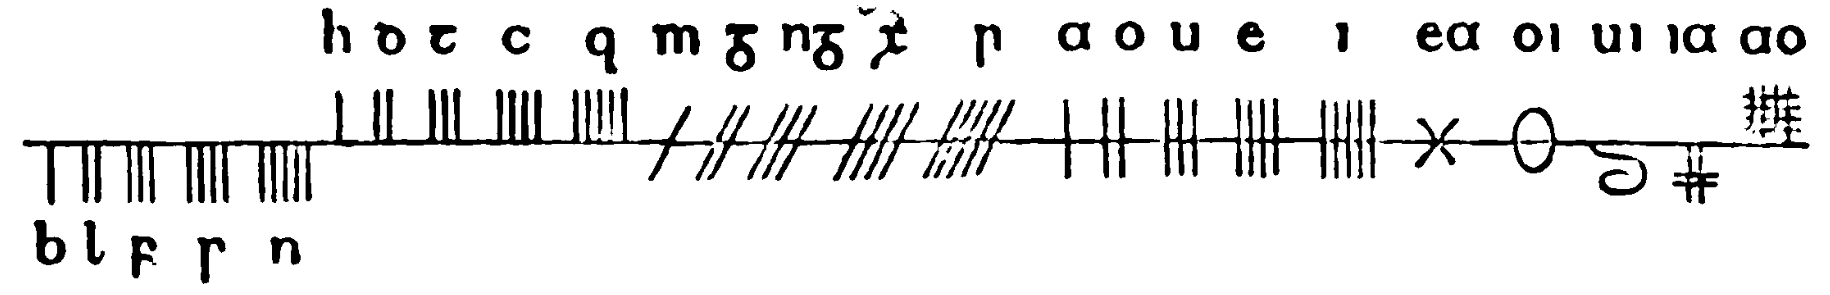
\includegraphics[width=\textwidth]{./images/ogham_craobh.png}

Here it is to be noted that the diphthongs beginning with \gaelicfont e, \normalfont as \gaelicfont ea, ei, eo, eoi, \normalfont are all distinguished by a cross ( $\times$ ) intersected by the stem line.
The diphthong \gaelicfont oi \normalfont is marked by a circle bisected by the line.
The diphthongs and triphthongs beginning with \gaelicfont u, \normalfont as \gaelicfont ua, ui, uui, \normalfont are all marked by a curve TODO below the line.
All the diphthongs and triphthongs beginning with \gaelicfont i, \normalfont as \gaelicfont ia, io, iu, iui, \normalfont are denoted by two strokes drawn below the line, with two others intersecting them at right angles.
All the diphthongs beginning with \gaelicfont a, \normalfont as \gaelicfont ao, ae, ai, \normalfont are marked by four parallel strokes intersected at right angles by four others placed above the line.
The letter \textit{z} (\textit{ts} or \textit{dz}) which has been decidedly borrowed from the Roman alphabet is represented by a curve of this form TODO (``representans inuolutam Draconis caudam'') intersected by the stem line, thus, TODO.
A short line drawn parallel to the stem line TODO represents the consonant \gaelicfont p\normalfont; and \gaelicfont q\normalfont, which was unquestionably borrowed from the Roman alphabet, and used by the Irish to stand for \gaelicfont cu\normalfont, is indicated by five strokes drawn perpendicular to the stem line.---See O'Molloy's \textit{Grammatica Latino-Hibernica}, pp. 135--142. 

In a MS. in the British Museum (Clarendon 15), various Oghams are described, such as Dinn-Ogham, in which the name of the letters are borrowed from those of hills ; En-Ogham, in which they are borrowed from those of birds; Dath-Ogham, from colours; Cell-Ogham, from churches, \&c.; but these are evidently contrivances of later ages.

The ancient Irish also used an obscure mode of speaking, which was likewise called Ogham, and is thus described by O'Molloy: ``Obscurum loquendi modum, vulg\`o \gaelicfont Ogham\normalfont, Antiquarijs Hiberni\ae satis notum, quo nimirum loquebantur syllabizando voculas appellationibus litterarum, dipthongorum, et tripthongorum ipsis dumtaxat notis\footnote{Gramatica, p. 133}".
To this mode of speaking distinct reference is made in the following entry in the \textit{Annals of Clonmacnoise}, as translated by Connell Mageoghegan, in the year 1627: 

``A.D. 1328. Morish O'Gibelan, master of art, one exceeding well learned in the new  and old laws, civille and cannon, a cunning and skillfull philosopher, an excellent poet in Irish, an eloquent and exact \textit{speaker of the speech, which in Irish is called Ogham} and one that was well seen in many other good sciences: he was a cannon and singer at Twayme, Olfyn, Aghaconary, Killalye, Enaghdown, and Clonfert; he was official and common judge of these dioceses; ended his life this year.''

But if the Irish are obliged to resign all claims to letters in the time of paganism, they can still historically boast of having writers among them before the general establishment of Christianity in the fifth century; for we must infer, from the oldest lives of St. Patrick, that there were several christian bishops in Ireland on Patrick's arrival; and we learn from St. Chrysostom, in his \textit{Demonstratio quod Christus sit Deus}, written in the year 387, that the ``British Islands, situated outside the Mediterranean sea, and in the very ocean itself, had felt the power of the divine word, churches having been founded there, and altars erected\footnote{
    S. Chysostom, Opp. tom. i. 575, B, Ed. Bened. 
    Καὶγὰρ αἱ Βρετανικαὶ νῆσοι, αἱ τῆς θαλάττης ἐκτὸς κείμεναι ταύτης, καὶ ἐν αὐτῷ οὖσαι τῷ ὠκεανῷ, τῆς δυνάμεως τοῦ ῥήματος ἤσθοντο· καὶ γὰρ κἀκεῖ Ἐκκλησίαι καὶ θυσιαστήρια πεπήγασιν.
}''.


But the most curious information respecting the literate character of Ireland before St. Patrick's time, is derived from the accounts of Celestius, who was certainly an Irishman, and the favourite disciple of the heresiarch Pelagius. 
St. Jerome, alluding to a criticism of Celestius upon his Commentaries on the Epistle of St. Paul to the Ephesians, thus vents his rage against this bold heretic: 


``Nuper indoctus calumniator erupit, qui Commentarios meos in epistolam Pauli ad Ephesios reprehendendos putat.
Nee intelligit, nimia stertens vecordia, leges Commentariorum, \&c.,..... nec recordatur stolidissimus, et Scotorum pultibus  % unsure if the choice of 5 periods here was significant or just a form of ellipsis so i have preserved it
pr{\ae}gravatus, nos in ipso dixisse opere: non damno digamos, imo nec trigamos, et si fieri potest octogamos: plus aliquid inferam, etiam scortatorem recipio p{\oe}nitentem\footnote{
    Hieron. Prolog. in lib. i. in Hieremiam. Opp. ed. Vallarsii, tom. iv.
}.'' 

And again, in the \textit{proemium} to his third book on Jeremiah, St. Jerome thus more distinctly mentions the native country of Celestius: 
``Hie tacet, alibi criminatur; mittit in universum orbem epistolas biblicas, pri\`us auriferas, nunc maledicas: et patientiam nostram, de Christi humilitate venientem, mal\ae conscienti\ae signum interpretatur.
Ipseque mutus latrat per Alpinum [al. \textit{Albinum}] canem grandem et corpulentum, et qui calcibus magis possit s{\ae}vire, qu\`am dentibus.
Habet enim progeniem Scotic\ae gentis, de Britannorum vicini\^a: qui, juxta fabulas P\"oetarum, instar Cerberi spirituali percutiendus est clav\^a, ut {\ae}terno, cum suo magistro Plutone, silentio conticescat\footnote{
    Prolog. i. lib. iii. in Hieremiam.
    Some, however, think that the heretic Pelagius is here alluded to.
    See Vallarsius, not. in loc.
    Opp. S. Hieron. tom. iv. who confounds, both here and in his note on the passage last quoted, the \textit{Scotia} of St. Jerome with the modern Scotland: not knowing that Ireland was the only country called Scotia in St. Jerome's time. 
}." 

We learn, however, from Gennadius (who flourished A.D. 495), that before Celestius was imbued with the heresy of Pelagius, he had written from his monastery to his parents three epistles, in the form of little books, containing instructions necessary for all desirous of serving God, and no trace of the heresy which he afterwards broached.
The words of Gennadius are as follows: 

``Celestius antequ\`am Pelagianum dogma incurreret, im\`o adhuc adolescens, scripsit ad parentes suos de monasterio 
Epistolas in modum libellorum tres, omnibus Deum desiderantibus necessarias. Moralis siquidem in eis dictio nil vitii postmodum proditi, sed totum ad virtutis incitamentum tenuit\footnote{
    Gennadius de Script. Eccl. c. 44 (inter Opp. B. Hieron. Ed. Vallarsii, tom. ii.)
}.''

It is conjectured\footnote{
    Moore's \textit{History of Ireland}, vol. i. p. 208.
} that these letters were written by Celestius from the monastery of St. Martin of Tours, in the year 369.
But be this as it may, if Celestius, while a youth, wrote epistles from a foreign monastery to his parents in Scotia, in the neighbourhood of Britain, we must conclude that his parents could read them, and that letters were known in Ireland, then called Scotia, at least to some persons, at the close of the fourth century.
For further historical reference to Celestius, and his master Pelagius, the reader is referred to Ussher's \textit{Primordia}, p. 205, \textit{et sequent}., and O' Conor's \textit{Rerum Hibernicarum Scriptores, Prolegomena}, p. lxxxiii. 

There are also inscriptions still extant to which we may appeal in proof of the early use of letters in Ireland.
The following, which is of undoubted antiquity, is a copy of the 
Roman alphabet, inscribed on a stone at Kilmalkedar, in the west of the county of Kerry.
An accurate representation of this inscription is given by Mr. Petrie, in his \textit{Essay on the Ecclesiastical Architecture and Round Towers of Ireland}\footnote{
    Transactions of the Royal Irish Academy, vol. xx. p. 133
}, and is inserted here by permission of the author.

\noindent
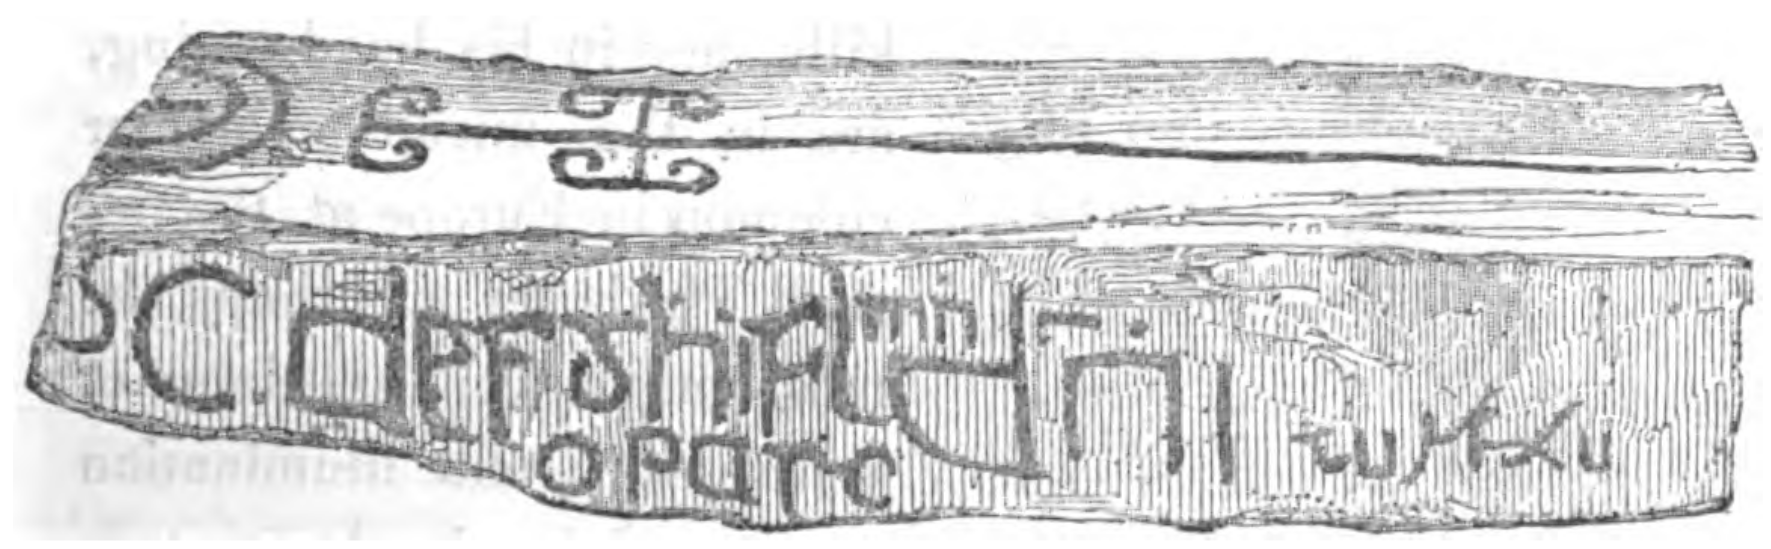
\includegraphics[width=\textwidth]{./images/petrie_inscription.png}

But there is a still older inscription, perhaps the oldest extant, which remains on the monument of Lugnathan, the nephew of St. Patrick, at Inchaguile, in Lough Corrib, county of Galway: of this a fac-simile is also given in Mr. Petrie's work, p. 164, and is here inserted.
It contains the following words, in the Roman characters of the fifth century: 

\begin{center}
    \LARGE \gaelicfont LIE LUGNAEDON MACC LMENUEH. \\
    \large \normalfont ``\textsc{The Stone of Lugnaedon Son of Limenueh}''
\end{center}


\end{document}

The oldest Irish manu- 
script extant in Ireland is the 
Book of Armagh, now in the 
possession of the Rev. Mr. 
Brownlow. It contains a copy 
of the Gospels, and some 
very old Lives of St. Patrick ; 
the characters are clearly a 
slight modification of the 
Roman alphabet, with a few 
Greek characters in the titles 
of the Gospels. 

The Books of Durrow 
and Kells, in the Library of 
Trinity College, Dublin, said 
to be coeval with St. Columb- 
kilJe, and in his handwriting, 
are in the uncial character 
common in Europe at the pe- 
riod. The latter is, perhaps, the 
most magnificent specimen of 
penmanship and illumination 
now remaining in the western 
world. 

There is another manu- 
script of great age preserved 
in the Library of Trinity Col- 
lege, Dublin, called Liber Hymnorum^ containing several 
ancient hymns in Latin and Irish, of which work there is ano- 
ther copy in the College of St. Isidore at Rome. This, though 
evidently not so ancient, nor so exquisitely beautiful, as those 


Introduction. liii 

already mentioned, is in the same character, and suflBciently 
proves that the Irish letters are immediately derived from the 
Roman alphabet. Ussher, in a letter to Vossius, expressed 
his opinion that this manuscript was then a thousand years 
old, but I think he increased its age by a century or two. 

The manuscript of the Psalter, preserved in the Cathacb, 
or Caah, a beautiful reliquary, now the property of Sir 
Richard O'Donnell, is also very probably coeval with St. 
Columba, if indeed it be not in his handwriting. This most 
curious box and reliquary has been deposited, by the public 
spirit and good taste of its owner, in the Museum of the 
Royal Irish Academy. 

A fac-simile of an Irish passage in a manuscript at Cam- 
bray, has been recently published by Charles Purten Cooper, 
Esq., from which it would appear that the manuscript is 
probably of the eighth century. The character looks as old 
as that of any manuscript we have in Ireland, and diflfers from 
any of them that I have ever seen, in the form of the letter p, 
which is thus (f ). Pertz, who has read the passage tolerably 
well, considering that he does not understand a word of the 
language, ascribes this manuscript to the ninth century. 

The next oldest Irish manuscript remaining in Ireland is 
probably the Book of Leinster, preserved in the Library of 
Trinity College, Dublin (H. 2. 18.) ; and next in order of time 
I would rank Leahhar na h- Uidhri, in the Library of the 
Royal Irish Academy, which was transcribed by Maelmuire 
Mac Cuinn na m-bocht, at Clonmacnoise, in the twelfth 
century. Next may be classed the Leabhar Breac of the 
Mac Egans, the Books of Lecan and Ballymote, and a host 
of others compiled from more original manuscripts, in the 
fifteenth century. The characters in these are of a more 
angular form than those in the more ancient manuscripts^. 

^ Mons. Adolphe Pictet of Ge- June, 1835, seems to incline to 
neva, in a letter addressed to the the opinion that we had no writ- 
late Edward O'Keilly, dated 24tli   ten documents in Ireland before 


liv 


Introduction. 


Specimens of alphabets from the most important of these 
ancient manuscripts, forming a series, nearly complete, from 
the sixth to the seventeenth century, will be found in the an- 
nexed plates. They have been drawn, from the original 
manuscripts, by George Du Noyer, Esq., one of the Fellows 
of the College of St. Columba. 


Section 2.— Of the Writers on Irish Grammar. 

Having now noticed the bardic accounts of the antiquity 

of letters among the Irish,  and the authorities which prove 

the  existence  of learning in  Ireland before St. Patrick, we 

shall next give some account of the labours of those who have 


the fourth or fifth century, or at 
least that this is the most remote 
period to which -written docu- 
ments can be traced. The que- 
ries which this learned philologer 
proposes in this letter are very 
curious, and should not be omit- 
ted here : 

" 1°. La seconde edition de 
votre dictionnaire a t-elle paru, 
ou doit elle bientot paroitre ? 

" 2°. Existe-t-il quelque bon 
dictionnaire anglais-irlandais ? 

"3°. A-t-on publie, depuis 
O' Conor, ou doit-on publier pro- 
chainement, quelques textes an- 
ciens, soit poetiques, soit histo- 
riques, soit philologiques ? Com- 
ment I'academie royale d'Irlande 
n'encourage-t-elle pas la publi- 
cation des textes anciens des 
Brehon laws, des poemes encore 
existans de Cenfaolad,de Eochoid, 
de Tanaide, de Maelmuire, etc, 
du glossaire de Cormac de Pur- 
aicheapt de Fortchern, etc. ? 

" 4°, N'a-t-on retrouve aucun 
fragment de traduction de la 
Bible en ancien irlandais, dont 
ou puisse fixer la date avec quel- 


que certitude ? par ancien ir- 
landais j' en tends la langue telle 
qu'elle existoit anterieurement 
au dixieme siecle et depuis le 
4ieme ^^ gieme ^poque la plus re- 
culee, je crois a laquelle remon- 
tent les documens ecrits. 

" 5°. Connoissez-vous quel- 
que ouvrage de topographie sur 
I'Irelande ancienne ou moderne, 
qui renferme d'une maniere ex- 
acte et un peu complete les noms 
de lieux, fleuves, lacs, montagnes, 
provinces, tribes, etc, avec I'or- 
thographie irlandaise ? 

"Voila, monsieur, bien des 
questions. Je m'excuse encore 
de mon indiscretion en prenant 
la liberte de vous les adresser : 
I'interet de la science plaidera 
pour moi. Si vous etes assez 
bon pour vouloir bien m'aider 
de vos lumieres j'espere que mes 
travaux ne seront pas inutiles a 
la cause trop meconnue des 
etudes celtiques, et reveilleront 
sur le continent un interet nou- 
veau pour les restes venerables 
de la litterature du plus ancienne 
peuple de I'Europe." 


Introduction. Iv 

written on Irish grammar. The first work of this kind men- 
tioned by the Irish writers is Uraicecht na n-Eiges, or Pre- 
cepts of the Poets. This treatise is attributed to Forchern, 
or Ferceirtne, the son of Deaghaidh, from whom the Deagads, 
or Clanna Deaghaidh, of Munster, are descended. It is said 
to have been written at Emania, the royal palace of Ulster, 
in the first century, but was afterwards interpolated and en- 
larged at Derryloran, in Tyrone, about the year 628, by 
Cennfaeladh, the son of Ailill. Copies of this work, as re- 
modelled by Cennfaeladh, are preserved in the Books of Lecan 
and Ballymote, in the Library of the Royal Irish Academy, 
and a more ancient one, on vellum, in the British Museum, 
which the Author has recently perused. This work contains 
rules for poetical compositions, and is rather a prosody than 
a regular grammar. In a paper manuscript, in the Library 
of Trinity College, Dublin (H. 1. 15), is a larger work, called 
Uraiceacht^ which gives genders and inflections of nouns, and 
various orthographical and etymological rules ; but this work 
is a compilation of comparatively modern times. 

There are several short treatises on Irish grammar, in ma- 
nuscript, by various writers in the seventeenth century, in the 
Library of Trinity College, and one, by O'Mulconry, in that 
of St. Sepulchre's, Dublin ; and we learn from the monument 
of Sir Mathew De Renzi, at Athlone, who died in 1635, that 
he composed a grammar, dictionary, and chronicle, in the 
Irish tongue^. 

The first Irish book ever printed, with instructions for 
reading Irish, was John Kearney's " Alphabeticum et Ratio 
legendi Hibernicam, et Catechismus in eadem Lingua, 1571, 
8vo." The only known copy of this curious and rare book is 
preserved in the Bodleian Library, Oxford*. 

z  See  Statute  of Kilkenny,    12, note «. 
edited by Mr. Hardiman for the * The Catechism is a Transla- 

Irish Archaeological Society,  p.   tion into Irish of the Catechism 


Ivi Introduction. 

The first printed Irish grammar is that of the Rev. Francis 
O'Molloy, written in Latin, and entitled " Grammatica 
Latino-Hibernica, nunc compendiata, — Authore Rev. P. Fr. 
Francisco O'Molloy, Ord. Min. Strict. Observantise, in 
Collegio S. Isidori S. Theol. Professore Primario, Lectore 
Jubilato, et Prouincise Hibernise in Curia Romana Agente 
Generali. Romse, Typographia S. Cong, de Propag. Fide 
1677." It contains 286 pages, 12mo., and is divided into 
twenty-five chapters, of which the first nine treat of the let- 
ters; the tenth, eleventh, and twelfth, of etymology, of which 
he treats but very slightly ; the thirteenth chapter is on the 
oghams and contractions ; and the remaining twelve, of the 
ancient Irish prosody, into which he enters very copiously. 

The next grammar of Irish which issued from the press 
was written by the celebrated antiquary Lhwyd. It was 
published in his ArchcBologia Britannica, and prefixed to his 
Irish-English Dictionary, Oxford, 1707. This work was 
extracted from O'MoUoy's, and from another work on Irish 
grammar, in manuscript, written by an anonymous author 
at Louvain, in 1669. It is somewhat more copious than 
O'Molloy's in the etymology, but is still very imperfect. He 
omits the defective or irregular verbs altogether, observing 
that they are very numerous, and that in conjugating them, 
"the common use and practice of the province, &c., is the 
only pattern." From the preface to his Dictionary, written 
in Irish, it appears that this great philologer knew almost 
nothing of the idioms of the Irish language, for he uses the 
English collocation in most of his sentences, which gives his 
Irish composition a strange, if not ridiculous, appearance. 

The next Irish grammar that made its appearance after 
Lhwyd's, was written by Hugh Boy Mac Curtin, a native of 


of the Church of England, which   Collects from the Book of Corn- 
is followed by some Prayers and   mon Prayer. 


Tntroduction. Ivii 

the parish of Kilcorney, near Corofin, in the county of Clare. 
It is entitled ''The Elements of the Irish Language, gram- 
matically explained in English, in fourteen chapters : small 
8vo. Lovain, 1728." It was reprinted with his English-Irish 
Dictionary, at Paris, in 1732. This work is much more 
copious that its predecessors, particularly in the etymology 
and syntax, on which the author has every claim to origina- 
lity. Of the irregular verbs he says, that they are very 
numerous, and that in the forming thereof, the common use 
or practice of the kingdom, or the distinct dialects of each pro- 
vince, is the only guide and rule. He omits prosody alto- 
gether. 

In 1742, Donlevy published, at Paris, his Irish- English 
Catechism, to which he appended instructions for reading the 
Irish language, entitled " The Elements of the Irish Lan- 
guage." This treats of orthography only, but it is by far 
the best treatise on the subject that had till then appeared. 
At the end, he says : " Such as desire to get more Insight 
into the Grammar-Rtiles of this Language^ may have recourse 
to the laborious M. Hugh Mac Curtin's Irish Grammar. 
The chief Difficulty of reading, or speaking Irish, consists in 
pronouncing oh, gh, and some Diphthongs and Triphthongs 
rightly ; but this is easily overcome by Practice, or a little 
instruction by the Ear ; whereby the Pronunciation of the 
Language will become agreeable, there being much Use made 
of Vowels, and little of Consonants, in it." 

No other Irish Grammar appeared after this till the year 
1773, when Vallancey published his, in quarto, with a preface, 
which tended to call attention to a subject then but little 
appreciated. Of this work he brought out an improved 
edition, in octavo, in 1782, with an " Essay on the Celtic lan- 
guage, shewing the importance of the Iberno-Celtic or Irish 
dialect to students in history, antiquity, and the Greek and 
Roman classics." 

h 


Iviii Introduction. 

This work is compiled from those already mentioned, and 
from O'Brien's remarks on the letters throughout his Irish- 
English Dictionary. The author has treated of the irregu- 
lar verbs more copiously and satisfactorily than any of his 
predecessors, and assures the learner that " they are not so 
numerous or more difficult than those of Latin, French, or 
English." His syntax, which is briefly dismissed in twelve 
rules, is much inferior to that of his predecessor Mac Curtin. 
On the whole, this work shews considerable research, and 
curious learning ; but it is more theoretical than practical, 
and better adapted to assist the comparative etymologist than 
the mere Irish student. It is by far the most valuable and 
correct of Vallancey's writings, and is doubtlessly the joint 
production of the avowed author and several native Irish 
scholars''. 

Shortly after Vallancey's, appeared Shaw's Gaelic Gram- 
mar, Edinburgh, 1778 ; but this is confined to the Erse or 
Gaelic of Scotland, and its merits are very questionable'^. In 
1801 appeared the first edition of a Gaelic Grammar, by 
Alexander Stewart, Minister of the Gospel at Moulin.   01 

*> The only other production from the History of the Hous« 

given to the world by Vallancey of O'Brien,  written  hy  the lak 

which shews much ability, is the Doctor John O'Brien, titular Bi- 

Law of Tanistry exemplified by shop  of Cloyne,  and  publishec 

the  Pedigree  of O'Brien ; but in the year 1774, by Col. Val 

this work  was written not by lancey." 

Vallancey, but by the Right Rev. " The Rev. Mr. SteAvart, in th( 

John O'Brien,  Roman Catholic Introduction to the 2nd editioi 

Bishop  of  Cloyne,  as  appears of his Gaelic Grammar, has  th( 

from a letter in the hand-writing following reference to this work 

of the Chevalier Thomas O'Gor- "I know  but  one publicatioi 

man, in the possession of Terence professedly of Gaelic Grammar 

O'Brien,  Esq.,  of Glencolumb- Avritten by a Scotsman ( Analysi 

kille,  in  the  county of Clare. of the Gaelic Language ; by Wil 

O' Gorman,  in  referring  to   a liam Shaw, A. M.) ; I have con 

genealogical extract  from Val- suited it also, but in this quar 

lancey's Collectanea, says: " The ter I have no obligations to ac 

above  genealogy  is  extracted knowledge." p. xiii. 


Introduction. lix 

this an improved edition was brought out in 1812, which is 
undoubtedly the ablest work on Gaelic grammar that ever 
appeared. 

In 1808 was published, in Dublin, an Irish Grammar, in 
octavo, entitled Upaicecc na ;5"e'3'%e, " A Grammar of the 
Irish Language," under the fictitious signature of E. O'C, 
which, in the Prospectus, is given in full as Edmund O'Connell; 
but the author, as many living witnesses can attest, was 
William Halliday, Esq., a solicitor in Dublin, who studied 
Irish as a dead language, and who died before he reached 
his twenty-fifth year, having produced this grammar in his 
nineteenth year. He derived much information from the first 
edition of Stewart's Gaelic Grammar, and from Messrs. Wolfe, 
O'Connell, and Casey, three Irish scholars, natives of Munster, 
with the latter of whom he commenced the study of the lan- 
guage in 1805, under the fictitious name of William O'Hara. 
In this work he rejects the modern Irish orthography as 
corrupt, and strikes out a new mode of classifying the declen- 
sions of nouns. His syntax is almost wholly drawn from the 
works of Mac Curtiil and Stewart, particularly the latter, 
whose arrangement and diction he has closely followed ; and 
indeed he could not have followed a safer model. However, 
he has pointed out some errors in the first edition of Stewart's 
Gaelic Grammar, which Stewart himself thankfully acknow- 
ledges and corrects in the second edition of his work, pub- 
lished in 1812''.   Haliday gives the ancient Irish prosody, but 

^ Stewart writes in the Intro- and derive some advantage from 

duction : " The Irish dialect of such Irish philologists as were 

the Gaelic is the nearest cognate accessible  to  me ;  particularly 

of tlie Scottish Gaelic.  An inti- O'Molloy,   O'Brien,  Vallancey, 

mate acquaintance with its voca- and Lhwyd.  To these very re- 

bles and structure, both ancient spectable names,  I have to add 

and modern, would have been of that  of the  Rev.  Dr. Neilson, 

considerable use.   Tliis I cannot author of ' An Inti'oduction  to 

pretend to have acquired.  I have the  Irish  Language,'  Dublin, 

not failed, however, to consult, 1808 ; and E. O'C, author of a 


Ix Ijitroduction. 

merely as shortened from O'Molloy, with, here and there, a 
few remarks of his own. This work, however, considering 
the early age^ and disadvantages of its author, must be re- 
garded as one of much merit ; it bears the stamp of taste, 
genius, and originality, not at all observable in the works of 
his predecessors. 

In the same year (1808) was published, in Dublin, " An 
Introduction to the Irish Language," by the Rev. William 
Neilson, D. D., 8vo. This grammar is the joint production of 
Dr. Meilson and Mr. Patrick Lynch, a native of the parish 
of Inch, near Castlewellan, in the county of Down. Mr. 
Lynch had a good practical knowledge of the dialect of Irish 
spoken in the east of Ulster, but was a rude scholar. The 
orthography, however, and grammatical rules, are adapted to 
this dialect, and not to the general language. The arrange- 
ment of the work is excellent, but it is to be regretted that 
the examples given to illustrate the rules are, for the most 
part, provincial and barbaric. 

In 1808 the Gaelic Society of Dublin published, in their 
Transactions, " Observations on the Gaelic Language, by 
R. Mac Elligott."   The same writer*^ also compiled an Irish 


' Grammar  of the  Gaelic  Lan- History" [of Ireland], " though 

guage,'  Dublin,  1808 ;  to  the originally   published   in   Mr. 

latter of Avliom I am  indebted Lynch's name,  was begun and 

for some good-liumoured stric- actually completed by the late 

tures, and some flattering com- William Halliday, Esq.,  whose 

pliments, which, however unme- much lamented death at the pre- 

rited, it were unhandsome not to mature age of 24, is a cause of 

acknowledge.'" p. xiii. heart-felt regret, not only to the 

^ Mr. Patrick Lynch,  the a\i- Gaelic Society, of which he was 

thor of the Life of St. Patrick, an active member,  but to  the 

has the following note in an ad- lovers of Irish literature in ge- 

vertisement  of his  works  ap- neral." 

pended to his Introduction to the ^ For some account of the lite- 

Kiiowledge of the Irish Language : rary qualifications of Mr. Mac El- 

" N. B. The new translation of ligott,  the reader is referred to 

the  first  volume  of  Keating's a pamphlet published in London, 


Introduction. Ixi 

Grammar, which is still extant in manuscript, in the possession 
of his daughter, Mrs. Ryding, of Limerick, but was never 
printed. He was a native of the county of Kerry, a region 
in which they studied classics, " even to a fault," in his time, 
and was for many years a classical teacher in the city of 
Limerick, where he created a high taste for classical and 
polite literature. 

The next year (1809) ushered into light " A Practical 
Grammar of the Irish Language," by the Rev. Paul O'Brien. 
This is, perhaps, the worst attempt hitherto made to explain 
the principles of this language. The author was a native of 
Meath, and a man of some learning ; but the visionary cha- 
racter of his mind disqualified him for the important task of 
writing a grammar of an ancient and neglected language. 
He does not appear to have had any acquaintance with Irish 
history or topography, or with any of the correct ancient 
Irish manuscripts. There are many specimens of his poetry 
in the native Irish preserved, but they exhibit no merit, 
except the mere power of stringing together long compound 
words in jingling rhyme, without poetic genius, or strength 
of thought. His Irish Grammar is the production of his old 
age ; and the late Mr. James Scurry says, in his Review of 
Irish Grammars and Dictionaries, published in the fifteenth 

ill 1844, by his pupil, the Rev. collection of annals,  and  other 

Jonathan Furlong,  in reply to inestimable  monuments.    The 

certain observations by Dr. D. books of Lecan and Ballymote, 

Griffin, of Limerick, in the life of and the^ebap bpec,or 'speckled 

Gerald  Griffin,  the  celebrated book,' of Mac Egan are in the 

novelist. We learn from O'Flana- archives of the Royal Irish Aca- 

gan that Mr. Mac Elligott had demy ;  and  there  are  besides 

got some valuable Irish manu- several valuable tracts in private 

scripts in his possession in 1808. hands throughout the island, of 

In euiimerating the collections of which those in the possession of 

Irish manuscripts known to him, tlie learned M'Elligott, of Lime- 

O'Flanagan writes :  " The Che- rick, are not the least worthy of 

valier O'Gorman,  now living in estimation," — Transactions of the 

the county of Clare,  has a rare Gcdic Society ofDablin, p. 235. 


Ixii Introduction. 

volume of the Transactions of the Royal Irish Academy, that 
" it is not to be taken as a fair specimen of the vigour of his 
intellect, or the extent of his learning." 

In 1813 Mr. John O'Connell, of the parish of Tuath na 
Droman, near Caherciveen, in Kerry, published at Cork an 
Irish translation of F. Paul Segnary's " True Wisdom," to 
which he prefixed short " Instructions for reading Irish," 
which are very correct. This translation is a curious speci- 
men of the dialect of the Irish spoken in Kerry. 

In 1815 was published, in Dublin, a small grammatical 
tract, entitled '^ Foroidcas Ghnath-Ghaoidheilge na h-Eir- 
eandf An Introduction to the Knowledge of the Irish Lan- 
guage as now spoken," by Patrick Lynch, Secretary to the 
Gaelic Society of Dublin. This little work contains some 
very valuable remarks on the pronunciation and genius of the 
Irish Language, although it cannot be considered as entitled 
to the name of a grammar. Mr. Lynch was a native of the 
county of Limerick ; he kept a classical school at Carrick-on- 
Suir in 1800, and afterwards removed to Dublin, where, for 
many years, he taught the classical languages, French and 
Hebrew. He wrote small works on grammar, chronology, 
astronomy, geography, and history ; but the most celebrated 
of his works is his " Proofs of the Existence of St. Patrick," 
written chiefly to refute Ledwich's assertions. This work 
was published in Dublin, in 1810, and contains short " Direc- 
tions for reading Irish." Mr. Lynch was of the Milesian 
Irish race (and wrote his name Patruic O'Loingsigh), and not 
of the Galway tribe of that name. 

In 1817 appeared " A Compendious Irish Grammar," by 
Edward O'Reilly, annexed to his Irish-English Dictionary. 
This is chiefly compiled from the Rev. Paul O'Brien's Gram- 
mar, and partakes of all its faults and defects. His system of 
making the initials of nouns the foundation of the declensions, 
in imitation of O'Brien, is quite absurd, as the tables of ter- 


Introduction. Ixiii 

minational changes, given in both grammars, sufficiently 
shew. The author was a man of strong mind, good memory, 
and studious habits, but had little or no acquaintance with 
the classical languages, or with any, except English. He 
learned Irish as a dead language, and had not commenced 
the study of it till he was more than thirty years of age; but 
by laudable perseverence, and strong powers of intellect, he 
acquired a considerable knowledge of the ancient Irish lan- 
guage and history. 

In 1820 was published, at Waterford, an Irish translation 
of John Baptista Manni's " Four Maxims of Christian Philo- 
sophy," by Mr. James Scurry, of Knockhouse, in the barony 
of Iverk, and county of Kilkenny. To this is prefixed " An 
Introduction to the Irish Language, containing a comprehen- 
sive Exemplification of all the alphabetical Sounds, and their 
corresponding English Sounds, as a further Illustration of 
them, as far as could be effected by the Substitution of English 
characters." 

This treatise is valuable, as giving the pronunciation 
which prevails in the diocese of Ossory, with which the writer 
was most intimately acquainted. 

In 1828 Mr. Scurry published, in the fifteenth volume of 
the Transactions of the Royal Irish Academy, " Remarks on 
the Irish Language, with a Review of its Grammars, Glos- 
saries, Vocabularies, and Dictionaries ; to which is added a 
Model of a comprehensive Irish Dictionary." In this paper, 
p. 55, the author says, " that he had prepared for press a 
grammar, both theoretical and practical, formed on the genius 
of the language, the result of many years' consideration of the 
subject, which he had been deterred from publishing, from the 
little encouragement works of that nature had met with from 
the public." Mr. Scurry was a respectable farmer, and though 
his education was imperfect, he was a man of so vigorous a 
mind that he acquired an extensive knowledge of philology 


Ixiv Introduction. 

and general literature^. He died in Dublin in 1828, and his 
body was buried in the church of Kilpecan, near the village 
of Mullinavat, in the county Kilkenny, where it lies without 
a monument to exhibit even his name. 

Various other compilations, and abstracts from these 
grammars, have since been published ; but the limits of this 
preface would not permit a particular description of them. 
The largest work of this kind was published in Dublin, in 
1841, and compiled for the Synod of Ulster, by S. O'M. 
Dr. Mason, Librarian of the King's Inns, Dublin, also com- 
piled an Irish Grammar ; but it is to be regretted that he has 
adopted the system of O'Brien and O'Reilly to a considelfable 
extent. The Rev. Mr. Nangle, of Achill, has also brought 
out a second edition of Neilson's Irish Grammar, with some 
judicious corrections. And Mr. Owen Connellan, who was 
employed for many years in the Royal Irish Academy, to 
transcribe the Books of Lecan and Ballymote, for the Royal 
Library, has recently published a small work on Irish Gram- 
mar, with examples from Irish MSS., not to be found in any 
of the works of his predecessors. He also gives the pronun- 
ciation which prevails in the northern part of Connaught, 
which will be found very useful, in preserving for posterity 
the local peculiarities of the Connacian dialect. 

Some works have also been written on the grammar of 
the Gaelic of Scotland, by Armstrong and Munroe ; but they 
contain nothing original, the Rev. Alexander Stewart having 
exhausted the subject, in his very excellent Gaelic Grammar, 
published in 1812. 

8 The Author of these pages cal grammar.  He was the first 

became   acquainted  with  Mr. that induced the Author to study 

Scurry in Dublin, in the year thegrammatical works of Harris, 

1826, and found that, although Ward, Home Tooke, Pickburne, 

he had but slight acquaintance and Fearns, and the antiquarian 

with Latin or Greek, he had still productions of Baxter,  Davies, 

a sound knowledge of philosophi- and Vallancey. 


Introduction. Ixv 

Section 3. — Testimonies to the Value of the Study of Irish. 

The testimony of such writers as have mentioned the Irish 
language, in ancient and modern times, may be now adduced, 
in order to shew the importance and value of the language as 
a branch of philological study. 

Ledwich^ quotes Irenseus (a. d. 167), Latinus Pacatus 
Drepanus (a. d. 361), and Sidonius Apollinaris (a. d. 472), in 
proof of his asseition, that the ancients "branded the Irish 
language with the harshest expressions for its barbarism. But 
even though it were clear that these writers meant what we 
now call Irish, we should receive their testimony with some 
allowances, for the Romans described as barbarous the lan- 
guages of all nations not civilized by themselves, except the 
Greeks. 

Our own Adamnan, however, who was born in the year 
624, and was one of the best Latin writers of his age, ac- 
knowledges, in his modest preface to his Life of St. Columba, 
that his own Latin style was inelegant, and that the Scotic 
language was to be classed with different other languages of 
the external nations.   His words are : 

" Beati nostri Patroni {Christo suffragante) vitam descrip- 

^ Antiq. p. 325. I have not the number of seventeen letters, 
been able to find any thing of so different in their powers, 
this kind m S. Irenseus. Charles names, and arrangement, from 
O'Conor of Belanagare, thinks those of the Greeks and lio7nans ? 
that the original harshness of the Evident it is, that without inter- 
Celtic must have been softened courses of this nature on the 
down in Ireland by a communica- Continent, and perhaps after- 
tion between the Phoenicians and wards in this island, our old in- 
the ancestors of the Scots. " How habitants might be considered 
else," he asks, " the number of (as some have laboured to repre- 
P/icenician words discovered in sent them) the most barbarous, 
their language ? By what other as they were the remotest, in the 
means but a communication with west of Europe." — Origin and 
the Phoenicians could they im- Antiquities of the ancient Scots, 
prove and harmonize their own prefixed to Ogygia Vindicated, 
unsonorous Celtic ? From what p. xxxviii. 
other people could they obtain 


Ixvi Introduction. 

turus, fratrum flagitationibus obsecundare volens : imprimis 
eandem lectures quosque admonere procurabo ; ut fidom dictis 
adhibeant compertis ; et res magis quam verba perpendant, 
quae (ut sestimo) inculta et vilia esse videntur, meminerintque, 
Regnum Dei non eloquentise exuberantia, sed in fidei floru- 
lentia constare : et nee ob aliqua Scoticce, vilis videlicet lin- 
guae, aut humana onomata, aut gentium obscura locorumve 
vocubula (quae, ut puto, inter alias exterarum gentium viles- 
cunt linguas) utilium, et non sine divina opitulatione gestarum 
despiciant rerum pronuntiationem*." 

By this passage we are to understand that Adamnan re- 
garded the Scotic language as one of those which had not 
received the polish of the classical languages ; and in this 
light must all the vulgar languages of Europe be viewed, till 
they were cultivated during the last four or five centuries, 
and received terms of art from the Latin and Greek. 

Tirechan also, in his " Annotations on the Life of St. Pa- 
trick," in giving a reason for having composed a portion of 
them in the Scotic language, though he was able to write the 
Roman language, says the Scotic names of men and places 
{^^ qualitatem non habentia") would not sound well in Latin 
composition. But the same could be said of the Hebrew, 
Persian, Arabic, and all the eastern languages ; the proper 
names of which would not sound well in a Latin sentence, as 
wanting the necessary terminations, and could not be even 
pronounced by an ancient Roman, or a modern Italian. 

In  the  seventeenth  century,  Archbishop  Ussher  pro- 
nounced the Irish to be a language both elegant and copious^ 

* See  Ussher's  Sylloge,  1st guage,  ascribed to a prelate o 

edition, p. 42 ; Parisian edition, equal dignity in our own time 

p. 29.   See also  Colgan's  and " The Irish language is a barba 

Pinkerton's editions  of Adam- rous jargon, in which all the dis 

nan's Life of St. Columba. cordant sounds to be heard ii 

J A curious  contrast to this the farm-yard  are  mixed  up 

account is afforded by the follow- there is the drawling running 0 

ing description of the Irish Ian- one  note  into  another  of tli 


Litroduction. Ixvii 

" Est quidem lingua hsec [scil. Hibernica], et elegans cum 
primis, et opulenta : sed ad rem isto modo excolendam (sicuti 
reliquas fere Europ^e Linguas vernaculas intra hoc sseculum 
excultas videmus) iioiidum extitit hactenus qui animum adji- 
ceret*^." 

Stanihurst, the uncle of Archbishop Ussher, a Roman 
Catholic priest, although he wished the Irish language not to 
be used in the English Pale, still does not venture to condemn 
it, as uncouth or barbarous. 

" Idem ipse locus a. me olim erat tractatus, in Hibernite 
descriptione, quam dictione vernacula edidi ; meaq. ibi dispu- 
tatio dedit sermonem inuidis, me laudes Hibernici sermonis 
minuisse. Sed in falsa hac criminatione suam produnt male- 
uolentiam, non redarguunt meam. Nee enim ego tum ora- 
tione mea suscepi, linguam, cuius essem ignarus et insolens, 
minus considerate vituperando, adfligere : imo contra gra- 
vissimorum hominum auctoritas fidem mihi iamdudum fecit, 
eam, verborum granditate, dictionum concinnitate, atq. dica- 
citate quadam acutula redundare ; denique cum Hebraica 
lingua, communi conglutinationis vinculo." 

Campion, in his Historic of Ireland, written in 1571, thus 
speaks of the Irish language ; cap. iv. Dublin Ed. p. 17 : 

" The tongue is sharpe and sententious, offereth great 
occasion to quicke apothegmes, and proper allusions, where- 
fore their common Jesters, Bards, and Rymers, are said to 
delight passingly those that conceive the grace and propriety 

cock's crow, the  squall  of the archbishop must have uttered it 

peacock, the cackle of the goose, in jest.   For  though, like Sta- 

the  duck's  quack,  the  hog's nihurst, he has of course no wish 

gruut, and no small admixture to see the Irish language revived, 

of the ass's bray." — See Etruria still the authority of grave men 

Celtica, vol. i. p. 48, by Sir Wil- must have  convinced him  also 

liam Betham, where that writer that it is not so utterly savage as 

gravely comments upon the in- this description would make it. 
justice of this description of the " Ussher's  Letters,  by  Parr, 

language  of the  old Irish,  not Lett. 193, p. 486. 
perceiving  that  the  illustrious 


Ixviii Introduction. 

of the tongue. But the true Irish indeede differeth so much 
from that they commonly speake, that scarce one among five 
score can either write, read, or understand it. Therefore it is 
prescribed among certaine their Poets, and other Students of 
Antiquitie." 

The celebrated Leibnitz recommends the study of Irish, 
as useful in illustrating Celtic antiquities ; but he does not 
give any opinion as to the elegance or inelegance of the lan- 
guage.  His words are : 

" Postremo ad perficiendam, vel certe valde promovendam 
literaturam Celticam, diligentius linguae Hibernicse adjungen- 

dum esse, ut Lloydius egregie facere cepit Nam uti 

alibi jam admonui, quemadmodum Angli fuere colonia Saxo- 
num et Britanni emissio veterum Celtarum Gallorum Cim- 
brorum ; ita Hiberni sunt propago antiquiorum Britannicse 
habitatorum Colonis Celticis Cimbricisque nonnullis, et ut sic 
dicam mediis, anteriorum. Itaque ut ex Anglicis linguae 
veterum Saxonum et ex Cambricis veterum Gallorum ; ita 
ex Hibernicis, vetustiorum adhuc Celtarum, Germanorumque, 
et, ut generaliter dicam, accolarum oceani Britannici cismari- 
norum antiquitates illustrantur^" 

It would be tiresome to adduce here the praise of the Irish 
by the native writers™ ; but if the reader is curious to learn the 
opinion of a profound native scholar, who was acquainted 
with many other languages, he can turn to Dr. Lynch's 
Camhrensis Eversvs, pp. 16 and 159, where he will find a 
very curious account of the  avidity  that some persons pos- 

^ Collect. Etymolog., 0pp. vi. Dublin, a large quantity of her 

part 2, p. 129. ancient  records^  on  paper and 

"' Dean Swift, Rabelaius nos- parchment,  then in his Grace's 

ter, though fond of ridiculing the possession,  that  had  been  for- 

Irish people in most of his writ- merly collected and  carried off 

ings, yet, in a letter to the Duke from this country by the Earl of 

of Chandos, dated 31st August, Clarendon, during  the  time of 

1734, requests that nobleman to   his  government  here Spiffs 

restore to Ireland, by presenting Works hi/ Scott, vol. xviii. p. 224. 
to the Library of Trinity College, 


Introduction. Ixix 

sessed, in the writer's time, for studying Irish, and the feeling 
that existed to discourage such study ; also of the use of the 
language to preachers and antiquaries. 

Towards the close of the last century, Vallaneey described 
the Irish in the following laudatory terms : 

" The Irish language is free from the anomalies, sterility, 
and heteroclite redundancies, which mark the dialects of 'bar- 
barous nations ; it is rich and melodious ; it is precise and 
copious, and affords those elegant conversions, which no other 
than a thinking and lettered people can use or acquire"." 

The Rev. William Shaw, in his Gaelic Dictionary (Lon- 
don, 1780), calls the Irish language "the greatest monument 
of antiquity, perhaps, now in the world. The perfection," 
he says, " to which the Gaelic arrived in Ireland in such re- 
mote ages is astonishing." Alluding to the Irish MSS. of 
Trin. Coll. Dublin, which he calls "sealed books," he makes 
the following observation : " Whilst I surveyed and examined 
them, and looked back to the ancient state of this once blessed 
and lettered island, they produced emotions easier conceived 
than produced." 

The same writer (Gaelic Gram., Edinb. 1778) has the fol- 
lowing observations on the state of learning in Ireland : 

" Whilst Roman learning, by the medium of a dialect of 
the Saxon, now flourished in Scotland, the Gaelic and Roman 
in some degree grew together in Ireland, which, for some 
centuries, was deemed the greatest school for learning in 
Europe. There letters and learned men, from all countries, 
found a secure retreat and asylum. Its happy situation, how- 
ever, did not perpetuate these blessings. Ireland was invaded 
by the Danes, and, in a subsequent age, made subject to the 
kings of England. Though there were English colonies in 
Ireland, the Gael of that country enjoyed their own laws and 
customs till the reigns of Elizabeth and James I., when the 

" Essay on the Gfelic Language, p, 3. 


Ixx Introduction. 

English laws were universally established. Then, for the 
first time, the Gselic ceased to be spoken by the chiefs of 
families, and at court ; and English schools were erected, 
with strict injunctions, that the vernacular language should 
no longer be spoken in these seminaries. This is the reason 
why the Iberno- Gaelic has more MSS. and books than the 
Caledonian. In Scotland there has been a general destruc- 
tion of ancient records and books, which Ireland escaped. It 
enjoyed its own laws and language till a later date, while the 
Scots- English very early became the language of North 
Britaino." 

About the same time, the learned Dr. Samuel Johnson 
expressed the following opinion of the Irish language and 
literature, in a letter to Charles O' Conor, of Belanagare : 

" What the Irish language is in itself, and to what lan- 
guages it has affinity, are very interesting questions, which 
every man wishes to see resolved, that has any philological or 
historical curiosity. Dr. Leland begins his history too late. 
The ages which deserve an exact inquiry, are those times, 
for such times there were^ when Ireland was the school of the 
West, the quiet habitation of sanctity and literature." 

The celebrated Edmund Burke was anxious to preserve a 
knowledge of the Irish language, for the purpose of proving 
or illustrating that portion of Irish history which precedes 
the period of Anglo- Irish official records. In a letter toVal- 
lancey, dated 15th August, 1783, he says : 

" All the histories of the middle ages, which have been 
found in other countries, have been printed. The English 
have, I think, the best histories of that period. I do not see 
why the Psalter of Cashel should not be printed, as well as 
Robert of Gloster. If I were to give my o{)inion to the 
Society of Antiquaries, 1 should propose that they should be 
printed in two columns,  one Irish and the other Latin, like 

° Introduction, p. ix. 


Introduction. Ixxi 

the Saxon Chronicle, which is a very valuable monument, 
and, above all things, that the translation should he exact and 
literal. It was in the hope that some such thing should be 
done, that 1 originally prevailed on Sir John Seabright to let 
me have his MSS., and that 1 sent them by Dr. Leland to 
Dublin. You have infinite merit in the taste you have given 
of them in several of your collections. But these extracts only 
increase the curiosity and the just demand of the public for 
some entire pieces. Until something of this kind is done, 
that ancient period of Irish history, which precedes official 
records, cannot be said to stand upon any proper authority. 
A work of this kind, pursued by the University and the 
Society of Antiquaries, under your inspection, would do 
honour to the nation." 

Mons. Adolphe Pictet, of Geneva, in our own time, has 
written the following account of the importance of the Irish 
language in his work, De VAffinite des Langues Celtiques 
avec le Sanscrit : 

^^ L'irlandais, par son extension, sa culture, et I'ancien- 
nete de ses monuments ecrits, est de beaucoup le plus impor- 
tant des dialectes gaeliques. Sans entrer ici dans des details 
qui nous meneraient trop loin, je me bornerai li dire que ces 
monuments sont fort nombreux qu'ils embrassent I'histoire, 
la philologie, la legislation, la poesie, qu'ils datent surement 
pour la plupart du 10*^ au 14® siecle, et que quelques uns 
remontent tres probablement jusqu'aux 7*^ et 6^ p." 

But to collect other testimonies of this kind would exceed 
the limits which must necessarily be imposed on the present 
publication. 


Section 4. — Of the Dialects of Irish. 

A few remarks must now be made on the dialects of the 
Irish language.   Keating informs us, from the ancient tradi- 

P Avant-projyos, pp. viii. ix. 


Ixxii Introduction. 

tions of the bards, that Fenius Farsaidh ordered Gaedhal, 
the son of Eathor, to divide the Gaedhelc language into five 
dialects, namely, Bearla Feine^ Bearla Fileadh, Bearla 
eadarscartha^ Bearla Teibidke^ and Gnath-bhearla. On 
this subject, Thaddseus Roddy, of Crossfield, near Fenagh, 
in the county of Leitrim, wrote as follows, in the year 1700*1 : 

" I have several volumes, that none in the world now can 
peruse, though within twenty years there lived three or four 
that could read and understand them all, but left none behind 
absolutely perfect in all them books [sic\^ by reason that they 
lost the estates they had to uphold their publique teaching, and 
that the nobility of the Irish line who would encourage and 
support their posterity, lost all their estates, so that the anti- 
quaryes posterity were forced to follow husbandry, &c., to 
get their bread, for want of patrons to support them. Honos 
alit artes. Also the Irish being the most difficult and copious 
language in the world, having five dialects, viz. the common 
Irish, the poetic, the law or lawyers' dialect, the abstractive 
and separative dialects : each of them five dialects [«^c] being 
as copious as any other language, so that a man may be per- 
fect in one, two, three, or four of them dialects \sic\, and not 
understand almost a word in the other, contrary to all other 
languages, so that there are now several in Ireland perfect in 
two or three of these dialects, but none in all, being useless 
in these times." 

Connell Mageoghegan, who translated the Annals of 
Clonmacnoise in 1627, says that the " Fenechus, or Brehon 
law, is none other but the civil law, which the Brehons had 
to themselves in an obscure and unknown language, which 
none cou'd understand except those that studied in the open 
schools they had." 

'I The original (which consists the autograph of Roddy, and is 

of answers to questions proposed preserved  on paper,  bound  up 

to the writer, evidently by the with a vellum MS. in the Library 

great antiqxiary  Lhwyd),  is in of Trinity College, 11. 2. 16. 


Introduction. Ixxiii 

Vallancey thinks that there were but two dialects, the 
Feini and Gnath, i. e. the Fenian and the common ; and that 
the former was, like the Mandarin language of the Chinese, 
known only to the learned ; and that the science of jurispru- 
dence was committed to this dialect. These five dialects 
cannot now be distinguished with satisfaction. The Brehon 
Laws and other tracts are distinctly stated to be written in 
the Fenian dialect ; and Keating informs us that there are 
words from every primitive language in the Bearla Teibidhe, 
from which Vallancey assumes that it is the physician's dia- 
lect, because, 1 suppose, he found that the old medical Irish 
manuscripts contain words taken from various languages, such 
Latin, Greek, and Arabic ; but none of the medical Irish 
manuscripts are older than the twelfth century. The poets' 
dialect was the same in construction as the common language, 
except that the poets were constantly borrowing words from 
the Bearla Feme, and every other dialect"^. 

The dialects now spoken by the people differ considerably 
from each other, in words, pronunciation, and idiom, through- 
out the four provinces. The diflference between them is 
pretty correctly expressed in the following sayings or adages, 
which are current in most parts of Ireland : 

Ca blap jan ceapc aj an muimneac; 
Ud ceapr jan Blap aj an UUcac ; 
HI puil ceapc na blap aj an ^aijneac; 
Cd ceapc agup blap aj an g-Connaccac. 

" The Munsterman has the accent without the propriety ; 
The Ulsterman has the propriety without the accent ; 
The Leinsterman has neither the propriety nor the accent ; 
The Conaughtman has the accent and the propriety." 

"■ Of this we have a striking beth, by John  O'Mulconry,  of 

specimen in the Inauguration Ode Ardchoill, in the county of Clare ; 

Df Brian na Murtha O'Rourke, published by Mr. Hardiman, in 

composed in the reign of Eliza- his Irish Minstrelsy, vol. ii. p. 286. 

k 


Ixxiv Introduction. 

The antiquity of these national Irish sayings has not 
been determined ; but they must be of considerable age, as 
they are paraphrased by Lombard, in his work entitled De 
Regno HibernicB Commentarius, published in 1632, as fol- 
lows : 

*' Tertio notandum, quod hoc ipsum idioma sit vernaculum 
totius in primis Hibernise, tametsi cum aliquo discrimine, turn 
quoad dialectum nonnihil variantem inter diversas prouincias, 
turn quoad artificij obseruationem inter doctos & vulgares. 
Et Dialecti quidem variatio ita se habere passim sestimatur, 
vt cum sint quatuor Hiberniae prouincise (de quibus paulo 
infra) Momonia, Vltonia, Lagenia, Conactia, penes Conactes 
sit & potestas rectse pronuntiationis, & phraseos vera proprie- 
tas ; penes Momonienses potestas sine proprietate, penes 
Vltones proprietas sine potestate, penes Lagenos nee potestas 
pronuntiationis, nee phraseos proprietas^" 

There is another dialect known to some persons in the 
counties of Cork, Clare, Limerick, and Kerry, called Bear- 
lagar na saer,  or tradesman's jargon, of which Mr. Mac El- 

*Ledwich,who sees everything number of provinces, must have 

Irish with a jaundiced eye, refers diiFerent dialects and local pecu- 

to this passage of Lombard's, to liarities. Nothing but literature, 

confirm  his assertion,  that the and a public communication, can 

Irish was  a  barbarous dialect, form a standard dialect of a na- 

possessing " neither alphabetical tion ; and nothing can possibly 

sounds, words for ideas, ortho- prevent the language of a nume- 

graphy, or syntax."   He might, rous people from splitting into 

for the same reason, pronounce dialects. The older the language 

the Greek a barbarous jargon, is, and the more widely separated 

because it not only consisted of the tribes are, the greater will 

four principal dialects, the Attic, be the difference of the respective 

Ionic, Doric, and jEolic, but each dialects.  These facts being fairly 

of these dialects varied with the considered, it will appear that 

localities ; and in one colony of Ledwich's  observations  on  the 

Asia Minor, four different species different dialects of the Irish, are 

of the Ionic dialect were observa- nothing more than illiterate and 

ble.   Every  language,  of any impertinent criticisms, 
antiquity,  and  spread  over  a 


Introduction. Ixxv 

ligott, of Limerick, has given a few words and phrases in the 
Transactions of the Gaelic Society of Dublin, pp. 11, 12. 
This appears to be very like the slang of London, for as the 
latter preserves several Saxon words and phrases, which have 
become obsolete in the standard dialect of the English, and 
even in the provincial dialects, so the former preserves many 
ancient Irish words which have been obsolete in the spoken 
language throughout the provinces. 

But passing over all artificial dialects of poets, and slangs 
of artisans, we will find that the common living language of the 
country, like the provincial English in the different shires, 
divides itself into varieties of dialects, merging into each other 
by almost imperceptible degrees of approximation, and which 
it would be next to impossible minutely to describe. Donlevy 
has the following observation on the dialectic variations and 
incorrect modes of writing Irish prevalent in his own time 
(1742):— 

" Poets, not the Ancient and skilful, who took Pains to 
render their Poems sententious and pithy without much Clip- 
ping, but the Modern Makers of Doggrel Rhymes and Bal- 
lads ; to save Time and Labour, introduced the Custom of 
clipping and joining Words together, in order to fit them to 
the Measure of their Verses : Others, who wrote in Prose^ 
have, either in Imitation of the Poets, or through Ignorance 
and Want of Judgment, strangely clipped, and spelled, and 
huddled them together, as they are pronounced ; let the 
Pronunciation be never so irregular and defective ; not re- 
flecting, that di. Poetical Licence, even when justifiable, is not 
imitable in Prose ; or that Writing, as People speak or pro- 
nounce, is to maim the Language, to destroy the Etymology , 
and confound the Propriety and Orthography : fur, not only 
the several Provinces of Ireland, have a different Way of pro- 
nouncing, but also the very Counties, and even some Baronies 
in one and the same County, do differ in the Pronunciation : 


Ixxvi Introduction. 

Nay,  some Cantons pronounce  so  odly,  that the  natural 
Sound of both the Vowels and Consonants, whereof, even ac- 
cording to themselves, the Words consist, is utterly lost in 
their Mouths.   There are too many Instances of these Sup- 
pressions and Jumblings :  A few will suffice here to shew the 
Abuse thereof: rS""' TS^' r"^^' T^", instead of ajup jan, ajup 
gup, ajup me, or if "i^? ^"E^X ^" or ip cu : And all this Mangling 
and Confusion without so much as an Apostrophe (' ), to let 
the Reader see, that some Thing is left out.   Again, TTlac a 
narap, cuid a npip, instead of an Qcap, an pip: The poor Par- 
ticle an is divided in two,  and  one Half of it is joined to the 
subsequent Word, for no other Reason but that in the Pro- 
nunciation, the (n) comes fast and close upon the following 
Word, as it frequently happens in all living Languages : yet 
ought not to pervert,  or alter the Orthography, or Order of 
Speech in  Writing :  However,  from this Fancy of Writing 
as People speak, chiefly arise not only the  Mangling and 
Jumbling of Words, but also that puzzling Diversity found 
in the Writings even of those,  who know  the Language in 
Question, infinitly better than he, who has the Assurance to 
make these Remarks.   But, either they have not reflected, or 
rather were resolved to imitate their Neighbours, who curtail 
and confound the different Parts of Speech, with far greater 
Liberty than the Irish do ; for instance : I'll, you'll, he'll, &c. 
cou'dn't, sha'n't,  won't, don't, t'other, they're, ne'er, can't, 
ha'n't, and thousands of that Kind ; which, although very 
fashionable,  the judicious English  Writers look upon as a 
great Abuse, introduced only since the Beginning of King 
Charles the Seconds Reign ;  and  endeavour to discredit il 
both by Word and Example. 

" It is no Wonder then, seeing the English Tongue, al- 
though in the Opinion of all, it be otherwise much improved, 
is thus maimed and confounded, even in Prose, that a Lan- 
guage of neither Court, nor City, nor Bar, nor Business, evei 


Introduction. Ixxvii 

since the Beginning- of King James the First's Reign, should 
have suffered vast Alterations and Corruptions ; and be now 
on the Brink of utter Decay, as it really is, to the great Dis- 
honour and shame of the Natives, who shall always pass every 
where for Irish-Men: Although Irish-Men vixthoxxi Irish is an 
incongruity, and a great Bull. Besides, the Irish Language is 
undeniably a very Ancient Mother- Language, and one of the 
smoothest in Europe, no Way abounding with Monosyllables, 
nor clogged with rugged Consonants, which make a harsh 
Sound, that grates upon the Ear. And there is still extant 
a great Number of old \d\\xd\i\Q Irish Manuscripts, both in 
public and private Hands, which would, if translated and pub- 
lished, give great Light into the Antiquities of the Country, 
and furnish some able Pen with Materials enough, to write a 
compleat History of the Kingdom : what a Discredit then 
must it be to the whole Nation, to let such a Language go 
to Wrack, and to give no Encouragement, not even the 
Necessaries of Life, to some of the Few, who still remain, 
and are capable to rescue those venerable Monuments of 
Antiquity from the profound Obscurity, they are buried in ? 
But, to return to our Subject, so prevailing are Habit and 
Custom, that even those who are sensible of the Abuse of 
clipping and blending of Words, do sometimes insensibly slip 
into it*." 

The grand difference between the dialects of the present 
living language, consists in the position of the accent, and 
in the pronunciation of the grammatical termination ao in 
nouns and verbs, it being pronounced in Conaught and 
Ulster like oo, or urn, in all dissyllables and polysyllables, 
but varied in Munster, being sometimes pronounced like a, 
short, sometimes like ac, and sometimes like 05. The minor 
differences consist in pronouncing n like p when coming after 

' Christian Doctrine, pp. 504-507, Paris, 1742. 


Ixxviii Introduction. 

c, 5 and m, in the north and west. The Munster dialect is also 
remarkably distinguished by the pronunciation of 5 in geni- 
tive cases from c, and by throwing the primary accent on the 
second or third syllable when long. These peculiarities are 
pointed out in the Orthography and Prosody of the following 
Grammar with sufficient minuteness. 

The other dialects which shot off from the Gaelic of Ire- 
land at an early period, are the Erse, or Gaelic of the High- 
lands of Scotland, and the Manx, or primitive language of 
the Isle of Man. 

OF THE ERSE, OR GiELIC OF SCOTLAND. 

The Highland Gaelic is essentially the same as the Irish, 
having branched off from it in the sixth century ; but there 
are peculiarities which strongly distinguish it, though the 
spoken Irish of the north-east of Ulster bears a close resem- 
blance to it in pronunciation and grammatical inflections. 
The principal peculiarities of the Erse are the following : 

I. In the Terminations of Words. 

1. The frequent ending of the nominative plural in an^ 
as slatan^ rods ; mnathan, women ; mullaichean, summits ; 
clarsaichean, harps ; laithean, days. This is not unlike the 
old Saxon plural termination in ew, still retained in a few 
English words, as eyen, sheen, oxen, women"". 

2. In writing the personal terminations aipe, oip, and aio, 
or i6e, always air, and aiche, or iche, as sealgair, a huntsman, 
for realjaipe; dorsair, a doorkeeper, for the Irish Doppoip, 
or Doipfeoip ; coisiche, a footman, for coipibe^. 

3. In writing the termination ujab of progressive active 
nouns, always achadh, as smuaineachadh, for pmuamiujao ; 
gradhachadh, for jpabujab, 

" See Stewart's Gaelic Grammar, 2ad edit., pp. 54-57. 
» Id., p. 46. 


Introduction. Ixxix 

4. In writing the passive participle te hard, without vary- 
ing it to ra, ra, ce, re, as the Irish do. See this discussed 
more fully at pp. 205, 206. 

5. In writing the diminutive termination 05, always ag, 
as cuachag, a little cup, for cuacoj. This termination is also 
observable in the living language, and in the names of places 
in the north-east of Ulster. 

II. In the Beginning of Words. 

1. The genitive plural does not suflfer echpsis, as in Irish, 
for the Scotch Highlanders say nan cos, of the feet ; ?ian 
cea7in, of the heads; for the Irish, na 5-cop, na j-ceann. But 
nam is used before a labial, as nam bard, of the bards ; nam 

fear, of the men''. 

2. The possessive pronouns ar, our, hliur, your, do not 
cause eclipsis, for they write ar buachaill, our boy ; ar Dia, 
our God ; bhur cosa, of your feet ; for the Irish, up m-buach- 
aiU, ap n-t)ia, bap 5-copa. It should be remarked, however, 
that the eclipsing letters are often not used in the most ancient 
Irish manuscripts. 

The other peculiarities are less general, and consist in the 
inflection of the verbs, with a greater use of the auxiliary 
verb CO, and in the total absence of the p in the future tense 
of the indicative mood, and in the subjunctive mood ; also in 
the constant use of the negative ca, for the modern Irish nl, 
and the ancient noca, and in the strange orthography of some 
words, as chaidh, for cuai6, anciently coi6, he went ; thuirt, 
for Dubaipr, he said ; ghios, for d' piop, to know, see, or visit ; 
sometimes written bup in Irish manuscripts; seann, for pean, 
old. 

OF THE MANX DIALECT. 

The Manx is much further removed from the Irish ; and 
it is probable that the Isle of Man had inhabitants from Ire- 
** See Stewart's Gaelic Grammar, 2nd edit., p. 155. 


Ixxx Introduction. 

land long before the emigration of the Scots from Ireland to 
the coast of Argyle. Its words are principally obscured by 
being written as they are pronounced, without preserving the 
radical letters, as in the Irish. It also exhibits extraordinary 
corruptions, and approximations to the Welsh, of which the 
following are the most remarkable : 

1 . The nominative plural ends in n, as in the Erse and 
Welsh. 

2. A final vowel is lost, as " O Hiarn," for O Chijeapna, 
O Lord ! dooys, for oam-pa, to me, &c. 

3. ^ is added to progressive active nouns derived from 
verbs, as choyrt, for cup, putting. [This final t is also used 
in some words in Irish, as peicpmc, for peicfin. — See p. 200.] 

4. d is often put for 5, as dy bragh, for 50 bpac. 

5. Ms often written for c or 5, as tustey, for cuijpe, the 
understanding ; Jestor, for pepcop, the evening, &c. 

6. The final a, or e, of the passive participle is always 
dropped, as soillsit, foluit, for poiUpijce, poluijce, illumined, 
concealed. 

There are also many peculiarities of idiom, too numerous 
to be even glanced at here ; and some particles of constant 
occurrence are so strangely, though analogically different 
from the Irish, that an Irish scholar would find it difficult to 
understand a Manx book, without studying the language as 
a distinct dialect^. 

OF THE WELSH. 

It may not be out of place here to make a few observa- 
tions upon the analogies between the Cymric or Welsh and 
Scotic or Gselic dialects, they being considered by some as 

^ The reader is referred to ob- specimens of this  dialect  from 

servations  on  this  subject  by the  Manx  Book  of  Common 

Richard  Mac  Elligott,  in  the Prayer, London, 1767, with sug- 

Transactions  of the  Gselic So- gestions for restoring the pure 

ciety of Dublin, where he gives original orthography. 


Introduction. Ixxxi 

cognate, and by others, as belonging to a totally different 
family of language. That they are very remotely related is 
quite evident from the fact, that the Gaelic dialects of Ireland 
and Scotland, which separated from each other about the year 
of Christ 504, may be said to be still the same language : 
but that the Irish and Welsh were, at a still more remote 
period, the same language, will appear to any sober-minded 
philologer, on comparing the great number of words which 
are identical, or different only in analogical dialectic pecu- 
liarities in both languages, the almost perfect agreement of 
their mode of forming grammatical inflections, and even of 
their idioms, which are considered the soul of language. The 
number of words, not derived from the Latin, or Danes, in 
which they agree, having been already sufficiently shewn by 
Lhwyd and others, it will, therefore, be enough to point out 
here how far they agree in grammatical inflections ; for when 
his agreement is duly considered, it will, no doubt, impress 
the conviction, that nothing but relationship of people, and 
dentity of dialect, could have caused it, be the period of sepa- 
ration ever so remote. 

To a casual observer, the difference between the gram- 
Tiatical inflections of both languages will appear to be very 
^reat, because the Welsh have adopted more of the letters of 
he Roman alphabet, by means of which, and of certain other 
jombinations of their own invention, they write their words, 
hroughout all the grammatical inflections, exactly as they 
ire pronounced, without any regard to the preservation of the 
adical letters of the word ; whereas the Irish, who have not 
idopted all the Roman letters, always write their words with 
he initial letters of the roots, and give notice of the gram- 
natical influences, either by prefixing an adventitious conso- 
lant, or placing a mark of aspiration over or after the radical 
onsonants. To make this intelligible, let us take a word 
ommon to both languages, and place it under a grammatical 

1 


Ixxxii Introduction. 

influence, in which both agree : thus, bean, a woman ; Welsh, 
henyn. Now if we place the possessive pronoun do, thy, 
Welsh, dy, before this word, the radical letter b suffers what 
the Irish call aspiration, and they write do bean. But the 
Welsh, who do not observe the same orthography, although 
the change of pronunciation is nearly the same, write dy vemjn. 
In this particular both languages, considered orally, are the 
same, the difference existing merely in the system of writing. 
This being understood, let us next ascertain how far the 
initial changes by aspiration and eclipsis actually agree in 
both languages. 

In Welsh, the initial consonants of feminine nouns are 
aspirated (or, as the Welsh grammarians term it, become light) 
after the articles. 

In Irish, feminine nouns are always aspirated in the nomi- 
native singular after the article, as on bean, the woman ; 
pronounced an ven, or in van. 

In Welsh, after the possessive pronouns dy, thy, ei, his, 
aspiration takes place, as dy venyn, thy wife ; ei venyfi, his 
wife. In Irish, aspiration takes place after mo, my ; do, thy ; 
and a, his ; as mo bean, my wife (pronounced mo ven) ; do 
bean, thy wife ; a bean, his wife. It should be also re- 
marked, as a striking point of agreement, that ei, in Welsh, 
and a, in Irish, mean his, or hers ; and that when used to 
denote her's, they do not cause aspiration in either lan- 
guage : as, Welsh, ei henyn, her woman ; Irish, a bean. 
This point of agreement is so remarkable, that nothing but 
actual relationship of people and dialect could have originated 

ity. 

In Welsh, the initial consonants of adjectives are aspirated, 
or (as their grammarians phrase it) become light, when their 
substantives are feminine, as benyn vaur, a big woman.   In 


^ See Syntax, Rule xx v. p. 374. 


I 


Introduction. Ixxxiii 

Irish the same takes place in the nominative singular, as 
bean mop ; pronounced hen vore. 

In Welsh, certain prefixed particles cause aspiration, as 
rhy vyqan, very little ; ni qarav, I dB not love. In Irish the 
same prevails as a general principle of the language, as 
}io beaj, very little (ro veg) ; nl cajiaim, 1 do not love {ni ga- 
raimy. 

In Welsh, initial consonants are aspirated (made light) 
after all prepositions, except two. In Irish, many of the 
iprincipal prepositions cause aspiration^ 

The system of eclipsis and aspiration somewhat differs, the 
Welsh having more forms ; however, the agreement is so 
close, that nothing but original relationship could have caused 
it.  The following table will shew this agreement. 

h becomes m in Irish and Welsh by eclipsis, and v by aspi- 
ration. 

c ,, 5^ in Irish, and g and ngh in Welsh, by eclipsis, 
and ch by aspiration, in both languages. 

d ,, n in Irish and Welsh by eclipsis, and by aspira- 
tion 6 or 2/ in Irish, and dh (pronounced like 
the Saxon J?) in Welsh. 

/    ,,     V  in Irish by eclipsis, but wanting in Welsh. 

g ,, ng in Irish and Welsh, by eclipsis, and y by aspi- 
ration in Irish ; but the true aspirate is 
wanting in Welsh. 

p „ b in Irish, and b and tnh in Welsh by eclipsis, 
and ph by aspiration in both languages. 

t ,, d in Irish, and d and nh in Welsh, by eclipsis, 
and th in Welsh, and h in Irish, by aspiration. 

s ,y t in Irish, by eclipsis, and h by aspiration ; but 
both are wanting in the Welsh''. 

* See Composition, p. 336, and ''  See  Prichard's   " Eastern 

Syntax, Rule xxxix. p. 388. Origin of the Celtic Nations," 

' See Syntax, Rule xliv. page pp. 30, 31. 
392. 


Ixxxiv Introduction. 

Let us next see the analogy between the two languages 
in terminational inflections. In these we find an equally close 
agreement, as will appear from the following instances. 

1. The formation of the plural by attenuation, as Welsh, 
hard, a poet ; plural, beird : Irish, bap& ; plural, bdipo. 
Welsh, bran, a crow ; plural, brain : Irish, bpcm ; plural, 
bpnin. Welsh, gdr, a man; plural, ^%/-; Irish, peap ; plural, 
F'P- 

2. The formation of the plural by adding a vowel, as 
Wehh, penau ; Irish, cinou, heads^ 

3. The ordinals are formed in Welsh by the addition of 
ved, as safp, seven ; setpved, seventh. The ordinals in Irish 
are expressed by ma6, vadh, as peocc, seven ; peaccmao, 
seventh, pronounced sechtmdh. 

4. The terminations n and g are diminutive in Welsh, as 
dynyn, a manikin ; oenig, a lambkin. They have the same 
import in Irish, as bum'n, a little man ; uameoj (more usually 
uumfn), a lambkin ; cuileoy, a little fly. 

5. As expressive of an agent, the termination r is common 
to both languages, as, Welsh, 7norur, a seaman ; Irish (mu.p- 
peap, seaman), muilneoip, a miller. 

6. The termination og in Welsh adjectives is generally c 
in Irish, as Duw trugarog, a merciful God ; Irish, D,a cp6- 
caipeac. 

7. The termination vailr is used in Welsh adjectives to 
denote abounding, and map, in Irish, b.^ guerpvaur, costly; 
Irish, Uonmap, abounding ; p.onmap, abounding in wine. 

8. The present participle in Welsh ends in d ; in Irish, the 
progressive active noun.which stands for the present participle, 
generally ends in 6. r t- ^  , 

9. In what the Welsh grammarians call the first form of 
the verb, the third person singular is merely the verbal root, 

" See Chap. II. p. 83. 


Introduction. Ixxxv 

as carav, ca-t, car, from cam, to love. In Irish, the form of 
the verb in the past tense for the third person singular is the 
simple root of the verb. 

10. In Welsh, the third person plural ends in ant, ent, 
ynt. In Irish, in am, m, aoap. In this particular the Welsh 
is more like the Latin. 

11. In Welsh, the first person of the preter tense ends in 
is, or ais. In Irish, in ap (anciently aif), as in the following 
example oi cam, to love. 

SINGULAR. PLURAL. 

WELSH. laiSH. WELSH. IRISH. 

1. cerais,   capap. 1. carasom,   cappom, or capamap. 

2. ceraist,   capaip. 2. carasoch^   cap pib, or capabap. 

3. carodh,   cap. 3. carasant,   cappac, or capuoap. 

12. The passive voice is expressed in both languages by 
endings almost identical ; thus : 

WELSH.  IRISH. 

carier^ caprap, amatur. 

carid,   capa6,   amahatur. 

carir,   cappap, or cappaioep, amabitur. 

The Welsh has a greater variety of distinct terminations to 
express the persons than the Irish, but the Irish is far more 
distinct in the future tense, and in having a present and con- 
suetudinal tense in the active voice, which the Welsh wants 
altogether. 

The reader is referred to Dr. Prichard's valuable work, 
entitled " Eastern Origin of the Celtic Nations," for the 
theory of the personal terminations of verbs, where he shews 
that the personal endings of the verbs in the Welsh language 
are abbreviated forms of the personal pronouns. 

Whether this agreement of the two languages is owing to 
identity of race, or to an amalgamation of both nations in the 


Ixxxvi Introduction. 

third and fourth centuries, is a question not easily determined; 
but the probability is, that it is attributable to both. We are 
informed by Cormac Mae Cullenan, Bishop of Cashel, and 
King of Munster, in the ninth century, that Crimhthann 
Mor Mac Fidhaigh, Monarch of Ireland (of the Munster or 
Heberian line), subdued the Britons, and established Irish 
colonies, and erected royal forts, at Glastonbury and in Corn- 
wall, and throughout the country ; and that the Irish retained 
this power for a long time after the arrival of St. Patrick. 
It is not impossible, therefore, that it was at this period 
the Irish built the forts which the Welsh call Ceitir Guidelod, 
or forts of the Gaels, or Irish. Mr. Lhuyd says : " There 
are none of the Irish themselves, that I know of, amongst 
all the writings they have published about the origin and 
history of their nation, that maintained they were possessed 
of England and Wales ; and yet whoever takes notice of a 
great many of the names of rivers and mountains throughout 
the kingdom, will find no reason to doubt but the Irish must 
have been the inhabitants, when those names were imposed 
upon them'*." 

It is not true, however, that no Irish writers attribute 
to their ancestors the conquest of Britain, though I believe 
the notice of it had not been published in Lhwyd's time. 
It is stated as follows in Cormac's Glossary, voce Mogh 
Eime : — 

" At the time that the sway of the Gaels was great over 
the Britons, they divided Albion<= between them in holdings, 
and each knew the habitation of his friends ; and the Gaels 
did not carry on less agriculture on the east side of the sea 
than at home in Scotica [Scotia], and they erected habita- 

! Se^ ^rcWo^m Br., p. 7. Great Britain—See Ussher, Pri- 

Albion.-Thi, was originally mon/ia, and the Irish translation 
the  name  of all  the  island of   of Nennius. 


Introduction. Ixxxvii 

tions and regal forts there ; hide dicitur Dinn Tradui, i. e. 
the triple-fossed fort of Crimthann Mor Mac Fidhaigh, King 
of Erin, Alba, and as far as the Iccian sea ; et inde est Glas- 
timber na n-Gaedhal [Glastonbury of the Gaels], a large 
church which is on the brink of the Iccian sea, &c. And 
it was at the time of this division also, that Dinn Map Le- 
thain, in British Cornwall, received its name, i. e. Dun mic 
Leathain, for Map in the British is the same as mac. And 
they continued in this power for a long time after the arrival 
of St. Patrick. It was at this time Coirpre Muse was dwell- 
ing in the east [of the Channel], with his family and friends, 

&c.f" 

J. O'D. 


It is right to say a few words here respecting certain 
manuscript authorities frequently referred to, for examples of 
grammatical forms and inflexions, in the following work. 

1. The copy of Keating's History of Ireland, of which 
very great use has been made, and which is always quoted by 
its pages, is a manuscript in the Library of Trinity College, 
Dublin (H. 5. 26). It was purchased in London, for the 
College, a few years ago, by Dr. Todd, and proves to be the 
most accurate and valuable copy of Keating's work which is 
known to the Author. It is in the handwriting of John, son 
of Torna O'Mulconry, of the Ardchoill family, in the county 
of Clare, a most excellent Irish scholar, and a contemporary 
of Keating. 

2. The medical manuscript, by John O'Callannan, who 
was Mac Carthy Reagh's physician, sometimes quoted in the 
following pages, was the property of the Author, but is now by 


f For the original of this pas-   logical Society, note G, pp. 339, 
sage, see Battle of Magh Rath,   340. 
published by the Irish Archaeo- 


Ixxxviii Introduction. 

him deposited in the Library of Trinity College (H. 5. 27). 
It is a mere fragment, chiefly valuable for the age of its au- 
thor, who translated it from Latin into Irish, at Kilbritton, 
in the year 1414, when Donnell Reagh Mac Carthy Cair- 
breach was on his death-bed. 

3. The Irish manuscript transcribed in Ulster, in 1679, 
quoted as authority for the Ulster dialect of that period, and 
the extracts from the Book of Fermoy, the original of which 
is not now in Dublin^, were also the property of the Author, 
and are deposited in the Library of Trinity College (H. 5. 28). 
The latter of these manuscripts is in the handwriting of old 
Mr. Casey, formerly of Myler's Alley, Dublin, and was pur- 
chased for the Author by his friend, Myles John O'Reilly, 
Esq., of the Heath House, in the Queen's County, at the sale 
of the manuscripts of the late Edward O'Reilly, author of the 
Irish Dictionary. An account of the transcriber, Mr. Casey, 
will be found in Whitelaw and Walsh's History of Dublin. 

8 The Book of Fermoy was in the Author into whose hands it 

the possession of the Chevalier has fallen, or whether it is sti 

p'Wman,  at the close of the in existence, 
last century ; it is not known to 


.VNCIENT  IRISH  ALPIIAIU'TS 


X? 1 . From ihp Book of Kclln . 

I (i'^(Vullu•v ) 


lllf 111 11 U op (J 

X'."-M'i-oiu tbf Hook of l)ui-i-i>w..Viitojn-,\i)li of Sl ColuiiiUii . 
( U'-f' Cniuin- ) 

ah c "D d e^ tv p c, b 
1 I m u o p q n u 8 r 

G  U  V  V /^ 

S?;(. Fi-om ihc .Wloj-raph Cosiu'ls of SiMoliui;-. 
( 7 >!' ('.■utnn- 1 

A^ b  C  v'  d  e  f  -^  h  t  I   m   \i   o  p  i^ 
1^  ]•  r  II  V ^u 


X'.' v. From the l.il«'r Uvmuonuii. 
I !)oi-l()"MVulurv.» 


<) p (\ u s c u X ^ c 


AXClF.X'r  lUlSlI  .\l,rHABi;TS 


FlDiii  lilt'  l.iliiT  llviLiiionilii .    ''.  ('li;ii';ti-lri-. 

q .| n 1* - ii \ 

Frmii till' S;ime.    .'i'. Cliar/ic-lrr. 

,\  b  c  t^  c  f  5  1i  1  \  ni  u  0  y>  cj  \\ y 
c  u  V s-  ^_^ 

NV.'i. From tlii" I^alilnir a-i li-lhiullin- 

x\  b  c  r  0-  |_*  ^  1)  1  I  111   11   0  p 
>(  ]v  r  c T  -, 

NV Ci . Fixiiu rtic I'liiirtfrti in flip li<M)k ol' ivcll;». 
(l-l'!'C(iitun- > 

0  p  )\  y z  u 

NV7. FiMiu till' l$(x)k (if Lenrrai. 

( Li')' (Vnturv 1 

A   b  c  sv  V-  )^  F  1)  1  1  m  n  0  p 
M   n  s  ]•  r  u  y ^^ 

WJi.Fniiu llu> Aiitojjrjmh AiiiuJs !»!' v'' Four .\!;i,stiTS . 

A  b   C  1-^  ^-   I-"  T  1l  1   I   ni  n   0   p 


A GRAMMAR 


THE IRISH LANGUAGE. 


PART  I. 

ORTHOGRAPHY. 


CHAPTER I. 
CLASSIFICATION OF LETTERS. 

The modern Irish Alphabet consists of eighteen letters, 
arranged in the same order as their corresponding letters 
in the Roman Alphabet. They are as follows : a, b, 
c, t), e, p, 5, h, 1, I, m, n, o, p, p, p, c, u. The va- 
rious forms of these characters, as found in manuscripts 
of different ages, have been already shewn in the Intro- 
ductory Remarks. 

Of these letters a, e, 1, o, u are vowels, the rest are 
consonants. 

The vowels are divided into broad and small. The 
broad vowels are a, o, u ; the small e, 1. 

The consonants are either mutes or liquids. The 
mutes are b, c, o, p, 5, m, p, c ; the liquids I, n, p, p. 

B 


2 Classification of Letters. [parti. 

They are also divided into labials, palatals, and Unguals, 
from the organs of speech by which they are chiefly 
pronounced. The labials are b, p, m, p ; the palatals, 
c, 5, and the Unguals O, I, n, p, p, c. The letter h is 
not included in any of these divisions. 

Philosophical writers on comparative Etymology have divided 
the consonants of the Celtic dialects generally into surds and so- 
nants, and subdivided them into gutturals, palatines, linguals, 
,/\^ dentals, labials, semivowels, and sibilants ; but although these dis- 

tinctions have been found useful in comparative Etymology, it is 
not necessary to introduce them into a practical grammar. For a 
curious classification of the consonants of the Celtic dialects see 
Prichard's Eastern Origin of the Celtic J^ations, p. 129. 

The author several years since made a classification of the Irish 
consonants, according to Dr. Darwin's system of articulate sounds, 
as explained in his work called the Temple qfJVature, and drew up 
orthographical rules according to such a classification, but he has 
since been induced to reject these rules, in consequence of the no- 
velty of the terms, and to adopt the divisions which are in com- 
mon use. According to Dr. Darwin's system the Irish consonants 
would be divided thus : c, p, c are mutes, properly so called, as 
being perceptible stops of the vocal sound ; b, d, 5, orisonants, 
because they are preceded by a slight vocal sound formed in the 
mouth ; m, n, narisonant semivowels ; p, p, h, sibilants ; and I, p, 
orisonant liquids. The aspirated consonants would be thus clas- 
sified : b, 6, 5, sonisibilants ; c, p, p, r, simple sibilants ; and m 
a narisonant semivowel. 

Although this classification has not been adopted by any of the 
subsequent writers on the philosophy of articulate sounds, it is de- 
cidedly the most correct. 

It should be here remarked, that in ancient Irish MSS. conso- 
nants of the same organ, particularly b and p, c and 5, d and c, are 
very frequently substituted for each other, and that where the an- 
cients usually wrote p, c, c, the moderns write b, 5, o. 

D for c, as oap for cap, over, across. 


CHAP. I.] Classification of Letters. 3' 

c for D, as coclao for coDlao, sleep, MS. Trin. Coll. Dubl. 
(H. 3. 1 8.), p. 42 ; ecac for eaoac, Cormac's Gloss., voce ope cpeich. 

b for F, as beoil for peoil, flesh, Cor. Gloss., voce moj 6ime. 

c for 5, as cac, every, for ^ac; cloiceno for cloiseann, the 
skull, Cor. Gloss., voce ITloj 6ime. 

B for TTi, as noib for naoirii, saints. Ibid., voce Noip; abam for 
anmin, alone ; ap na bapac for ap na mapac, on the morrow, Vit. 
Moling. 

m for B, as a lenm, her child, for a leanb, Vit. Moling. 

p for b, as ma\\parz cac a ceile, for mapbam cdc a c^ile, Vit. 
Moling ; odip for ooib, to them. Annals of Ulster. 

p for b, as Qlpu for Qlba, Scotland, Cor. Gloss, (in v. Coipe 
bpecain) ; Coipppi for Caipbpe, a man's name. Ibid, (in v. ITIoj 
eime) ; cappac for capbao, a chariot, Ibid, (in v. Ope cpeirh). 

Nine of these consonants, namely, b, c, D, p, 5, m, 
p, p, c, are called aspirates, because in certain situations 
their primary or natural sounds are changed into aspi- 
rated sounds, as b, into b, i. e. the sound b into the 
sound V, &c., as will be presently shewn. 

Every consonant, whether in its primary or aspirated 
state, has a broad or a slender sound, according to the 
nature of the vowel which it precedes or follows. When 
it precedes or follows a broad vowel it has always a 
certain fixed broad sound, and when it precedes or fol- 
lows a slender vowel it has a fixed small or slender 
sound, which will presently be described. This influ- 
ence of the vowels over the consonants, which exists to 
some extent in every language, has given rise to a 
general rule or canon of orthography which distinguishes 
the Irish from all the European languages, namely, 
that every consonant, or combination of consonants, 
must always stand between two broad vowels or two 
slender vowels, as bpipim, 1 break ; molaio, they praise; 


4 Classification of Letters. [part i. 

co|ipop6a, corporeal ; not bpipaiD, moliD, coppepDa, 
or bpiopit), molet), coppopbe. 

O'Molloy, in his Grammatica Latino- Hibernica, published at 
Rome in 1677, explains this great canon of Irish orthography as 
follows, pp. 50, 51 : " Rursus obserua in voculis polisyllabis 
quibuscumque saltern ordinarie seruari debere regulam Hibernis 
tritam turn in scriptura, turn in sono, quae dicitur caol le caol, 
learhan le leachan, latine subtilis cum subtili, et larga cum larga. 
Hoc est dicere, si posterioris syllabse prima vocalis fuerit subtilis, 
similiter prioris seu antecedentis syllabse ultima vocalis debebit esse 
subtilis; pariformiter si larga, larga ; alias vitium erit turn in enun- 
ciatione, tum in orthographia : non tamen requiritur quod utraque 
vocalis semper ; sit eiusdem speciei, vel numeri, tametsi multoties 
contingat quod sint, sed sufficit quod ambse sint largae, vel ambae 
subtiles. Dixi ordinarie, nam exceptio datur de quibusdam pau- 
cissimis, vt uia, map, &c., latine, quam in quo., &c." 

Professor Latham, in his chapter on Euphony, and the permuta- 
tion and the transition of letters, notices this rule as a remarkable 
one in the Irish. His words are : " The Irish Gaelic, above most 
other languages, illustrates a Euphonic principle that modifies the 
Vowels of a word. The Vowels a, o, u, as seen in § 71, are Full, 
whilst i, e, y are Small. Now, if to a syllable containing a Small 
Vowel, as hmil^ there be added a syllable containing a Broad one, 
as aw, a change takes place. Either the first syllable is accom- 
modated to the second, or the second to the first; so that the 
Vowels respectively contained in them are either both Full or both 
Small. Hence arises, in respect to the word quoted, either the form 
htvaih?n, or else the form bwUim." — The English Language, 
p. 122. 

This rule, which has been so scrupulously adhered to by modern 
Irish writers, has been condemned as cumbrous by Vallancey, Stew- 
art, Haliday, Mac Elligott, and others, and it is certain that it is 
not always strictly adhered to in the ancient Irish manuscripts ; 
but the principle on which it is founded is observable in the oldest 
fragments of Irish composition remaining to us, as will appear from 
the specimens given in the Appendix to this work. 


CHAP. II.] Sounds of the Vowels. 


CHAPTER II. 

OF  THE  VOWELS. 


Section 1. — Of the Sounds of the Simple Vowels. 

All the vowels are sometimes long, and sometimes 
short or obscure. In the southern half of Ireland they 
have medial or diphthongal sounds between long and 
short, which have not been hitherto noticed, or at least, 
not sufficiently explained by Irish grammarians. These 
diphthongal sounds, not being strictly analogical, shall 
not be introduced into the text of this Grammar, with 
the exception of a few of the most prominent of them, 
lest they should perplex the learner ; but they shall be 
carefully described in the notes, in order to preserve the 
Munster pronunciation of the language. 

A long vowel is generally marked by an acute ac- 
cent, thus : bap, death ; mm, smooth. In the absence 
of this accent, it is understood that the vowel is short, 
as bap, the palm of the hand ; mm, meal. 

In words of two or more syllables the accent is ge- 
nerally on the first syllable, or root of the word, whether 
it be long or short, as pldnuijue, saved; coppopoa, 
corporeal. — See the Prosody, Chap. I., Sect. 1. 

There are no quiescent final vowels in this language, 
as in the English or French ; for although the final e in 
the words buibe, yellow, cpoibe, a heart,  and  such 


■^ 


6 Sounds of the Vowels. [part i. 

like, as pronounced at present, Is nearly quiescent, and 
looks as if it were merely intended, like the final e in 
English, to render the preceding vowel long, still we 
know from the oldest specimens of Irish poetry re- 
maining, that the final e in such words was distinctly 
uttered and accounted a syllable. 

The obscure sounds of the vowels prevail after the 
accented syllables, or when they are final in pollysyl- 
lables, as mopba, majestic ; njeapna, a lord. 

In this situation the vowels have so transient and indistinct a 
pronunciation that it is difficult to distinguish one broad or slender 
vowel from another, and hence in ancient manuscripts we find 
vowels substituted for each other ad libitum, as planui jce, saved, 
is written planaijce, pldnoijre, and pldnuijri ; where it is to be 
observed that the long accented a cannot be changed, but the ob- 
scure vowels are changed ad libitum, because the ear could not 
possibly distinguish the sound of one from that of the other. 
'Walker, in his observations on the irregular and unaccented sounds 
of the English vowels, has a remark somewhat similar to this. 
" If," he says, *' the accent be kept strongly on the first syllable of 
the word tolerable, as it always ought to be, we find scarcely any 
distinguishable diflference to the ear, if we substitute u ox o instead 
of a, in the penultimate syllable ; thus, tolerable^ toleroble, and 
toleruble, are exactly the same word to the ear, if pronounced 
without premeditation or transposing the accent for the real purpose 
of distinction," &c. 

However, in writing fldnuijre, and such other words as present 
many indistinct vowels, a fixed orthography should be preserved, 
and the form of the word to be adopted should be decided upon by 
observing the root and proper grammatical inflections or branches 
springing from it ; thus, from the root plan, safe, is formed plan- 
ujao, salvation, and the u in this form should be retained in the 
passive participle planuijre, and in all other derivatives springing 
from it, as rldnuijceoip, a saviour; planuisceac, sanative. 


CHAP. II.] Somids of the Vowels. 7 

Such as wish to become acquainted with the ancient MSS. 
should be informed that u before p may be written aup, ep, or ip, 
as upnaijre, prayers, which may be written aupnaijre, epnaijre, 
or ipnijre ; upoam, a scarcity, aupoam, epoam, ipoam. — See the 
remarks on the diphthong au. 

According to a principle of the language no number 
of vowels meeting in a word forms more than one syl- 
lable ; and therefore when many vowels come together 
an adventitious 6 or 5 is often thrown in between 
them to make a second syllable, and to serve the same 
purpose as a hyphen or a diseresis ; as t)0 beoaib, to the 
living, may be written 00 beobaib ; aiep, the air or sky, 
may be written aibep" ; but in ancient manuscripts these 
adventitious consonants are seldom, if ever, used, and 
we sometimes find four or five vowels together without 
any consonant intervening, as aieoip, of the air; 
aieupoa, caiuip, melodious". 

In modern Irish orthography no vowels are doubled in the same 
syllable, like ee or 00 in English ; but in the ancient manuscripts 
all long vowels are found doubled, as oee, gods; laa, a day; moo, 
greater, as " do pala laa nano mipi am oenap, I happened to be 
one day alone." — Battle of Magh Rath, p. 34. " ITloo a emeach 
oloap bir, his bounty is greater than the world." — Id. p. 52. This 
doubling of the vowels, however, does not in any way affect the 
pronunciation. 

In reading Irish, all consonants, whether primary 
or aspirated, must be pronounced according to their re- 
spective powers, as they shall presently be described, 
except such as are eclipsed, as pointed out in the table 

' See the  copy of Keating's   brary of Trinity College, Dublin, 
History of Ireland, by John Mac   p. 127, line 36. 
Torna O'Mulconry, in the  Li- '' Book of Fermoy. 


8 Sounds of the Vowels. [part i. 

of ecllpsis, and also the aspirated p, which is quiescent 
in every situation, and the aspirated 6 and 5 in the 
middle of words which are not compounds. It should be 
also remarked, that the aspirated t is but very faintly 
pronounced in the end of words, as plair, a chieftain ; 
bpeic, a sentence. 

Table of the Sounds of the Vowels. 

a. 

1. Q when long^ sounds like a in the English words 
callyfalU as Ian, full ; apt), high. 

In Meath and Ulster a long is pronounced like a in the English 
words mar ., father , as these words are pronounced hy Walker, and 
this is also the prevailing long sound of this vowel throughout the 
Highlands of Scotland ; hut it cannot be considered its true original 
sound. O'Molloy describes the long sound of this vowel as fol- 
lows : — " Hanc autem A efFeres cum Latinis large, ore scilicet de- 
ducto, flatu valentulo, suspensa modice lingua, et dentibus inuicem 
non tangentibus, ut amaoan, latine stultus^ — Gra77imatica La- 
tino-Hibernica, Romce^ 1677, p. 8. 

2. Q short, like a in the English word^^^, as anam, 
a soul; slap, green*". In the end of a word it is 
pronounced very obscurely, like a in the English word 
tolerable^ as ceapca, crucified or tormented ; Deanra, 
done ; m6p6a, majestic'^. 

*^ In  some  of the  southern tute o and u for it ad libitum, as 

counties a is pronounced in this Ullru for Ullra, the Ultonians; 

situation like a in the English odanco for oeanca,  done, but 

word what, as cape, thirst ; jap- this should not be permitted, as 

ca, acute. it would prevent the orthography 

<• As has been already remarked, of the language from becoming 

when a has this obscixre sound, fixed, 
it has been the custom to substi- 


CHAP. II.] Sounds of the Vowels. 9 

3. Qd and aj;, when immediately followed by a broad 
vowel, or by the consonants I, m, n, p, c, 5, are pro- 
nounced like the English word eye, or the German ei 
in ivein, as abapc, a horn ; ablacab, burial ; abpab, 
adoration ; Uaog, a man's name. 

This rule Isolds good throughout the southern half of Ireland, 
but it must be varied for the pronunciation of the north and west. 
In Connaught ao and aj, when followed by a vowel, have the sound 
laid down in the text, but when followed by I, m, n, p they are 
pronounced like a long (I), as aopao, adoration; aolacao, burial; 
aomcto, timber, which words are pronounced as if written apao, 
dlacao, dmao. In the north of Ulster ao and aj, followed by a 
vowel, or by the consonants c, 5, have a strange sound, not unlike 
ueeii closely and rapidly pronounced; but in the southern counties 
of Ulster, and in Meath, they are pronounced somewhat like ay in 
the English word mayor, as paoapc, sight; aoapc, a horn ; Caoj, 
a man's name, which words are pronounced in the north of Ulster 
nearly as if written paoioeapc, aoiDeapc, Uaoioeaj; but in the 
south of Ulster and in Meath, as if written paeoapc, aeoapc, 
Z^a^-oa^. Throughout the Highlands of Scotland this combination 
is pronounced nearly as in the north of Ulster, and Dr. Stewart 
says that " the sound has none like it in English." It would be 
now difficult to strike a medium between those various pronun- 
ciations, and point out what was the true original sound of this 
combination, but it is highly pi-obable that it was originally pro- 
nounced a long, as it is in some instances in Connaught at pre- 
sent. 

4. CXb in the end of words is pronounced in the 
south of Ireland like a in the English word general; 
as bualab, striking; Deanao, doing ; jlacao, receiving; 
peaca6, sin. 

This rule holds good in all monosyllabic words throughout 
Ireland ; but in dissyllables and polysyllables ao, in this situation, is 

C 


10 Sounds of the Vowels. [part i. 

pronounced like oo nasal throughout Connaught and Ulster. This, 
however, cannot be considered a sound of ao, but more properly of 
aril, which is the dialectic termination of most verbal nouns in 
Connaught and Ulster. For example, the word o^anao, doing, is 
pronounced in Connaught as if it were written DiojnaTh ; but this 
should not be considered the pronunciation of the form o^anao, 
which is peculiar to the south of Ireland, but of oinsnam, which is 
a form of this verbal noun found in very ancient manuscripts. Some 
Irish grammarians, who had but a local knowledge of the pronun- 
ciation of the language, not considering the dialectical variations of 
words, have given very odd sounds to some of the vowels and con- 
sonants, such as that of oo to the ao in question, and that of i to ^, 
which leads to much confusion and inaccuracy ; for it is in reality 
making a local peculiarity, or barbarism, the standard of a general 
principle of the language. 

The original pronunciation of ao and aj was in all probability 
like agh guttural, which is still partially preserved in the moun- 
tainous districts of the counties of Londonderry and Tyrone, as in 
'peao, it is ; cpuinneasao, a gathering, &c. 

/^, . 5. Q, when coming before the consonant m, or the 

double consonants II, nn, n^, in monosyllabic words, and 
before nr, nc in dissyllables, is pronounced in the south- 
em half of Ireland like the German au, or nearly like ow^ 
in the English word how, as am, time ; ball, a member ; 
pann, weak ; man^, a bag ; neancog, nettles ; pupean- 
cdn, a tune. But in the province of Ulster the a has its 
regular analogical short sound (2) in these situations^ 
6. Ct before b is pronounced in the southern half 

*= See the Prosody.   In some unknown in Ulster and in the 

parts of Connaught a before II, southern half of Ireland, and not 

m, and nn, has its natural long general even in Connaught ; it 

sound; as am, time, pronounced must therefore be regarded as a 

6m;  oall,  a blind  man,  pro- local peculiarity, 
nouuced odll ; but this sound is 


i'- 


CHAP. II.] Sounds of the Vowels. 11 

of Ireland like ou in the English word ounce, as abainn, 
a river ; cabaijic, giving ; labaipc, speaking. 

In the County of Kerry a, in this situation, has the regular 
diphthongal sound of a (5). But in Ulster it has the sound of o 
long, as abainn, a river; ^aBal, a fork ; jaba, a smith; jaBap, a 
goat, pronounced in Ulster at present as if written obainn, jdbal, 
joba, jobap. 

e. 

1. 6 long sounds like the Greek rjTa, or like e long 

in the French, and all languages except the English, as 

|ie, time ; y^e, six ; me, I. 

In English e long has evidently lost its original sound, it being 
now pronounced ee, like i long in all ancient, and most modern 
languages ; but e short still retains its original sound, as in other 
languages. E still keeps its ancient long sound in a few words, as 
where, there, ere, &c., in which words it exactly corresponds 
with e long in Irish. O'Molloy, in pointing out the primitive 
character of the pronunciation of the Irish vowels and diphthongs, 
thus exclaims : " Sistunt ergo Patrum, veterumque vestigijs, nee 
cum nouatoribus in vicinio mutant religionem Hiberni." — Gram- 
matica Latino- Hibernica, p. 46. 

2. G short is pronounced like e in the English word 
met, as Ouine, a man ; buile, madness. 

In the modern Irish orthography the vowel e never appears 
alone in the body of a word or syllable, but is always accompanied 
by other vowels ; but in the ancient Irish manuscripts it is often 
written singly, as p^p, grass ; pep, a man ; ben, a woman, for the 
modern p^ctp, peap, bean ; also pp^pe, of the firmament, for the 
modern ppeipe. — See notes under the diphthongs ea and ei. In 
the ancient manuscripts lu is frequently used for the final e short 
of the moderns, as " moo ocup aipoiu oloap cec pep," for the 
modern " mo ajup aipoe ma jac peap." — Battle of Magh Rath, 
p. 64. *' Q n-Dul uaic-piu" for "a n-oul uuic-pe." — Id., p. 68. 
" e.piu" for " eipe."_M, p. 110. 


12 Sounds of the Vowels. [part i. 

1. 

1. 1 long sounds like i long in all the ancient and 
modern languages, except the English, and like the 
usual long sound of the English e, or ee, as laid down by 
Walker, as mfn, smooth or fine ; ]if, a king*^. 

2. 1 short, like i in the English word mill, as mil, 
honey ; min, meal ; bile, an old tree. 

Before U and If the short i of the other provinces is pronounced 
like ei, very slender, in the south-east of Ireland, but in the south- 
west like i long, as milfe, sweeter ; mill, spoil ; pill, return; cill, 
a church. Neither of these sounds, however, can be considered 
analogical, though the former seems of considerable antiquity in 
the south of Ireland, and was highly prized by the poets for the 
sonorous jingles which it produced in their rhymes. It is made up 
of e-ee, not of a-ee, like the English i long. 

O. 

1. O long, like o in the English word more, as 
moji, great ; op, gold. 

Throughout Meath, and the adjoining counties of Ulster, o long 
is pronounced like a in hall, as 61, drink, pronounced all; o 
short exactly corresponds with it, and is pronounced like o in the 
English lot, sot ; but this must be regarded a great corruption. 

2. O short, always like o m the English words 
mother, brother, other, as copp, a body ; olc, evil^ 

•  ''^?'^^^ general long sound of i sound of the vowel o, as has been 

m Jl^nglisli is not that of a simple stated by all scientific writers on 

vowel   but  that  of a  perfect organic  sounds.   The  general 

diphthong ;  but  m  some  few short sound of o in English is 

words It has the pure sound of a the natural short sound of a long 

simple vowel, as in machine, &c. and broad, as in hall, all, &c. 
This  IS  the  natural  short 


CHAP. II.] Sounds of the Vowels. 13 

In monosyllables closed by the consonants U, m, nn, and in dis- 
syllables, when it is followed by 5, or 6, the vowel o is pronounced 
in the southern half of Ireland like ozt in the English word ounce, 
as poll, a hole; cpom, stooped; lorn, bare; ponn, desire; coja, 
selection ; poja, choice. These sounds were highly prized by the 
southern poets for their musical tone, although the inhabitants of 
the north and west of Ireland considered them unnatural and bar- 
baric. They are well exemplified in the following rhymes : 
" Ua ropann conn a' bojpao Hawk coip 
Q'p e gan fm, ^an irieaDj, jan blacaij." 

TfiUiam English. 
" 6a caol a com, a cpaoB-polc cpom 
CI5 ceacc 50 bonn lei na ppeacaib." 

John Claragh Mac Donnell. 
" t)ac an loca a'p 50pm na o-conn 
Q5 ceacc 50 coljac, copannac, cpom." 

Brian Merrijnan. 

In Ulster, Connaught, and Meath o, in these situations, has its 
snort sound, except before 6 and 5, where it is made long, as 
pojlaim, learning. 

It may be remarked here, once for all, that the principal dif- 
ference between the Munster and the other dialects of the Irish 
language consists in the diphthongal sounds of the vowels here 
pointed out. The Ulster and Connaught pronunciation is generally, 
and particularly in this instance, more analogical and correct, but 
the Munster dialect is more sonorous and musical. The natives of 
the different provinces, however, are much divided in their opinions 
of the different modes of pronunciation, each claiming his own to 
be the most mellifluous and the purest. — See Preface. 

U. 

1. U long^ like u in rule\ as iip, fresh; cul, the 
back. 

*" The usual sound of u in vowel, as it begins with the con- 
English is not that of a simple   sonantal sound of ^. 


14 Sounds of the Diphthongs. [part i. 

2. U short, like u mfull, bull, as ucc, the breast ; 
up fa, a prop. 

This is the natural short sound of u, and it will be necessary 
for the English scholar to remember here that the general short 
sound of u in English, as heard in tub, current, is really that of o 
short. In the ancient Irish manuscripts au is often written for the 
simple u of the moderns, as aupj-a for uppa, a jamb or prop ; au- 
6acc for uoacc, a will or testament ; aupoam for upoam, a portico. 


Section 1.— Of the Sounds of the Diphthongs. 

There are thirteen diphthongs in the modern Irish 
language, ae, ai, ao; ea, ei, eo, eu ; ia, io, lu ; oi ; ua, ui. 
Of these ae, ao, eu, la, ua, and most generally, eo are 
lonff: the others are sometimes long and sometimes 
short. Their sounds will be more particularly described 
in the following Table : 

Table of the Sounds of the Diphthongs. 

ae. 

Qe is always long, and sounds like ae in Latin, as 
pronounced by the continental nations, and like ay m 
the English word mayor, as aep, the air, the sky; lae, 
of a day ; pae, the moon. 

This diphthong is very seldom used in modern Irish orthogra- 
phy, and Dr. Stewart, who had no ancient manuscript authorities 
to refer to, seems to doubt (Grammar, p. 5) that it properly belongs 
to the Gaelic at all; but he is clearly in error, as it is generally 
used in the most ancient Irish manuscripts for the modern ao 
(which see).   O'Molloy, in 1677, describes its sound as follows: 


CHAP. II.]    Sounds of the Diphthongs. 15 

" Secunda biuocalis ae efFertur sicut a priscis olim Latinis, in 
Musce, scc^yt, et siiiiilibus, largius nempe quam si scriberentur cum 
e simplici, vt ael, latine calx." — Grammatica Latino- Hibernica, 

pp. 48, 49. 

ai. 

1. Qi, with the accent on a, sounds like a long and 
1 very short, as yccnl, a shadow; cdin, a tribute. 

The sound of this diphthong is varied in the provinces, accord- 
ingly as they pronounce the long a broad or slender. 

2. Qi shorti like a in art^ ai in plaid, or ai in the 
French word travailler, as baile, a town ; cailleac, a 
hag. 

This is the ancient and most analogical sound of this diphthong 
when short, and it now prevails throughout the southern half of 
Ireland ; yet in Ulster it is invariably pronounced like e short, as 
Qileach, the name of a place ; aiplinj, a dream, pronounced ellagh, 
esMing. The Rev. Paul O'Brien, who was a native of Meath, and had 
no general knowledge of the provincial variations of pronunciation, 
marks ai sliort as pronounced like i in the English word king., as 
ainjeal, an angel ; and it is true that it has this sound in some parts 
of Meath, but it should be regarded as a very corrupt sound of this 
diphthong, which is confined to a narrow district. Throughout 
Leath Mhogha, or the southern half of Ireland, this diphthong, 
when it comes before U, m, nn, 6, j, is pronounced aee, but some- 
what broader than the English i long, as aiU, a cliff; aimpp, 
time; |-naiDm, a knot; maijoean, a virgin; raiobpe, pride, osten- 
tation ; paioBpeap, wealth. The Munster poets of the last century 
delighted in jingles formed by this sound, as 

" O raiobpij me an paiobpeap ba jpeioni je le peacam." 

Donnell Mac Kei^nedy O'Brien. 

In Connaught, Ulster, and Meath, this diphthong is short in 
these situations, except before 6 and 5, when it sounds in Con- 
naught as in Munster, but in Ulster and Meath like ai in the 


16 Sounds of the Diphthongs. [part i. 

English word mam. It should be also observed here that the word 
rnaiom, a knot, which is properly pronounced snime in many parts 
of Mun'ster, is also pronounced in the south of Leinster, and several 
parts of Munster also, as if written rnaoini. 

In the preposition aip, upon, and a few other words, this diph- 
thong is pronounced like e in err, but the antiquity of this pronun- 
ciation is doubtful, as that preposition, in its simple form, is almost 
invariably written ap or pop in ancient manuscripts. 

ao. 

Qo Is pronounced in the south of Ireland like ay in 
the English word mayor, but in Connaught, somewhat 
like uee in the English word queen, as maoji, a steward; 
t)aop, dear. 

This diphthong is used in all printed Irish books, and is found 
in manuscripts of some antiquity, say four centuries ; but it never 
appears in the ancient Irish sepulchral inscriptions, nor in the ear- 
lier Irish manuscripts, as the Book of Armagh, the Liber Hymno- 
rum, Leabhar na h-Uidhri, the Book of Leinster, &c., but instead 
of it ae or oe are always used ; for which reason there can be little 
doubt that it was anciently pronounced as ae was among the ancient 
Latins. It still retains this ancient sound all over the southern 
half of Ireland, In Connaught it is pronounced somewhat like ea 
in the English word steal, but broader, and with something of a 
diphthongal sound, not unlike uee in queen. In Ulster and Meath 
it has a very odd sound, which may be represented by ueeu, closely 
and rapidly pronounced^. 

This diphthong was evidently introduced into Irish orthography 
to facilitate the adherence to the rule o^ Broad with a Broad, &c.. 


s O'MoUoy described the sound videlicet modice aperto, pug- 
of this diphthong as follows, in nante parce halitu cum superiori 
1677, but it is not easy to per- palato, reliquis omnino immotis, 
ceive which of the sounds here vt Qooh, quod proprium est no- 
laid doAvn he intends : " Cto ef- men viri, tametsi idem significet 
fertur  la to  mollique  sono,  ore quod Latine, ignis.' 


CHAP. II.]    Sounds of the Diphthongs. 1 7 

because ae, the diphthong which the ancients employed in its place, 
always gave the consonant which followed it a broad sound, and in 
the increments of words in which it occurred, broad vowels were 
always added, as poeji, paepa, where there would be an evident 
breach of the rule alluded to. Hence, when this great canon of 
Irish orthography began to be more strictly adhered to than it had 
been by the ancients, it was thought proper to change e into o, and 
write paop, paopa, which fulfils the rule. 

au. 

Qu is never used in the modern orthography, al- 
though frequently found in ancient manuscripts. Its 
pronunciation is uncertain; but it is often found in 
words now written with a u short, as aupcop for up- 
cup, a shot" ; aupoam for upoorh, a porch' ; laulgac 
for lul^ac, or loil^eac, a milch cow^ ; auDpepra for 
eaopeapr, or loobapc", an offering; Ctulell Qulom 
for Olioll Olum', a man's name ; Qiijaine forUgaine, 
a man's name". — See u long. 

ea. 

1. Ga long, exactly like ea in the English words 
hear, swear, tear, great, as ^eap, sharp ; peap, grass. 

The sound which ea represents in these words is the original 
and correct sound of that English diphthong, and is still preserved 
in speaking English by the uneducated classes in Ireland, where it 
had been introduced before the present affected change of its sound 
to ce took place in England.   In the south of Ireland the Irish 


^ MS. Trin. CoUege, Dublin, ^ MS. Trin. College,  Dublin, 

H. 2. 18. fol. 25. H. 3. 18. p. 361. 

' Book of Ballymote, fol. 245, a. ^ Cormac's Glossary, voce nioj 

i Cormac's Glossary, voce cli- Gime. 

rap-peo. "* Ibid, voce SanB. 

D 


*1 8 Sounds of th e Diphthongs. [part i. 

diphthong ea long is sometimes very corruptly pronounced ee-a, 
somewhat, but not exactly like ea in the English ^oxAfear ; but j 
this pronunciation, which never prevailed in any part of Connaught,; 
Meath, or Ulster, cannot be considered analogical, nor is it to bel 
approved of; and it is curious that while the natives of Munster 
use it in common conversation, they always reject it in repeating 
poems, songs, and prayers. 

2. Ga shorty like ea in the English words heart, 
hearth, hearken, as meap, respect ; cea]-, handsome. 

lo short is often used for ea short by writers of the seventeenth 
century.   In the ancient manuscripts a single e, or the character f, 
(which is only an elongated e), is always written instead of this 
diphthong whether short or long, as map, or mfp.for meap, finger; 
pep, or pfp, for p^ap, grass; map, or mfp, for maap, swift; cap, or 
Dfp, for oeap, handsome ; and it is curious that in the counties of Mo- 
naghan and Louth, and other parts of Ulster, this diphthong, when 
short, is pronounced like a single ej thus, the above words are pro- 
nounced mer, des, not mar, das, as in the other parts of Ireland. 
Some Irish scholars have thought that the character f, which fre- 
quently occurs in the Irish manuscripts, is a contraction for ea, 
but it can be proved that it stands for a simple a, as it is used to 
represent the Latin e in very ancient manuscript copies of the Gos- 
pels.— See some curious observations on this subject by Richard 
Mac EUigott of Limerick, in the Transactions of the Gaelic Society 
of Dublin, p. 26.  From the present pronunciation of the words 
in which this character is introduced in the ancient manuscripts, 
we must conclude that the ancients pronounced the consonant 
preceding it with a slender sound, and that following it with a 
broad sound ; and hence after the establishment of the great Gaelic 
orthographical canon of " Broad with a Broad," &c., an a was 
thrust in between the a and the following consonant, to mark its 
broad sound with more certainty, as peap, a man, for pap ; ceapc, 
just, for cape. 

Some have thought that it would improve the modern Irish or- 


CHAP. II.]    Sounds of the Diphthongs. 19 

thography to introduce the diphthong evi for ea, when long, as 
then ea would be always short and eu always long ; for example, 
for F^"Pj grass, to write peup. O'Molloy, in his Irish Catechism, 
and Duald Mac Firbis, in his Genealogical Book, have adhered to 
this distinction". 

In Munster and south Leinster eu in monosyllables ending in 
II, m, nn, and nj, is pronounced like the German au (aoo), as 
peall, treachery ; leam, with me ; sleann, a valley ; p^anj, slender; 
but in dissyllables, formed in the course of grammatical inflection 
from these monosyllables, it is pronounced short, as peaUaim, I 
deceive ; peanjan, a pismire ; an jleanna, of the valley ; except 
when a consonant follows, as meallca, deceived ; jleannca, valleys ; 
ceannca, a press, a support ; neanncoj, nettles ; jeallca, promised. 
These sounds, which the natives of Connaught, Meath, and Ulster 
abhor, are exemplified in the following rhymes : 

" Q h-aolcopp peanj, a p^iD cpob leabaip, 
Q caol-rpoij ceann, a oian, 'p a mailije." 

John Mac Donnell, surnamed Clarach. 

" t)o rpeij m6, ip peap, mo jpeann, 
Cd an cleip a n-aipio leam, 
]p baoc mo Beapr, ip paon mo neapc, 
tDo claon* p oo pcaip mo riieabaip." 

Andrew Magrath. 

It is necessary to remark here, for the information of such 
learners as wish to become acquainted with the ancient Irish wri- 
tings, that ea preceding p is often changed to au in old manuscripts, 
as aupoalca for eapoalca, certain; aupoam for eapoam, a porch, 
an apartment; and that these words are also found written with a 
u, as upoalca, upoam. Also that the ancients wrote lu short for 
the ea short of the moderns, as  " mopcu caca muiriupa'' for 


" Some Irish grammarians Connaught, and obtains in so few 
have marked another sound of words that it should not be con- 
ea, like ee in meek, as in o^an, sidered a sound of ea, but a pro- 
do, or make ; but this is very vincial substitution of to for that 
corrupt,  and confined to lower diphthong. 


20 Sounds of the Diphthongs.     [part i. 

« mopra jaca ma\reaya:—Batlle ofMagJi Rath, p. 100. " Fef 
cap plaiciupa," for " Feapcap plaireapa."— /<^. p. 122. 

3. Ga, with the accent on a, sounds like a in the 
English word father, as peapp, better; Seapp, short; 
pedpnog, the alder tree. 

There are very few words in the language in which this sound 
obtains, and even in these it is not generally adhered to throughout 
Ulster. It should be also remarked that the a is seldom written 
in ancient manuscripts, in which peppoe is written for the modern 
peappoe; pepnoj for peapnoj, &c. 

ei. 

1. Gi long, like ei in feign, reign, as leini, a leap; 
ceun, a step. 

2. Gi short, like-e \x\ ferry, as beip, bring; oeip, 

says ; ^eip, tallow. 

In Munster and south Leinster ei, in monosyllables ending in 
65, II, m. Dm, nn, 6, and 5, and in dissyllables, when it is followed 
by D, 5, or m, is generally pronounced like i long and slender in 
English, or the German ei, as peill, of treachery (gen. of peall) ; 
ceiU, a church ; jpeim, a bit or morsel ; peiom, use ; but in Con- 
naught, Meath, and Ulster ei in these situations (excepting only 
before U) is pronounced long, like ei in the English word reign. 
The Munster pronunciation of ei in these situations is exemplified 
in the following rhymes : 

" Cboip mdije na mapr nt puil meioip, 
O claoiDeao ap 5-ceap a j-ceiU." 

John O'Tuama. 

In ancient manuscripts a single e is often found for the ei of 
the moderns, as reap na jp^ne for reap na jpeine, the heat of the 
sun. — Battle of Magh Rath, p. 34, Duald Mac Firbis, in his ge- 
nealogical manuscript, and Peter Connell, in his Irish Dictionary, 
have, in many instances, rejected the diphthong ei and written a. 


CHAP. II.]    Sounds of the Diphthongs. 21 

single e in its place; and yet Haliday, who professes to restore the 
pure ancient orthography of the language, and rejects the diph- 
thongs ao, ea, eu, as modern and corrupt, retains ei as a pure an- 
cient diphthong ; for which he certainly has the authority of the 
Book of Lecan and other manuscripts of considerable antiquity. 


eo. 

1. Go longy like oa in shoal^ as peol, a sail; ceol, 
music ; but it must be borne in mind that the conso- 
nant preceding this is always slender, so tliat the e has 
its use. 

In Meath, Louth, and Ulster, this diphthong, when long, is 
pronounced like aw in shawl, and when short like o in mock. 
This arises from their manner of pronouncing o long, i. e. like a in 
call. 

2. Go short, like u in just, as Deoc, a drink ; 
eocai]i, a key. 

As this short sound of eo is found only in seven or eight words 
in the whole language, there is no necessity for placing an accent 
over the o when the diphthong is long, for the learner may con- 
sider it as always long. The words in which it is short are the 
following : oeoc, a drink; eocaip, a key; ©ocaio, a man's name; 
eoca, horses ; neoc, which ; peoc, a part ; and two or three others 
now obsolete. 

eu. 

Gu, always like ea long, as meu|i, a finger; rpeuD, 
a flock. — See Observations on ea. 

This diphthong is used by some modern writers for ea long, or 
the simple e long of the ancient manuscripts. Thus Duald Mac 
Firbis introduces it in the following lines, where the Book of Lecan 
has a single e : 


22 Sounds of the Diphthongs.     [part l 

'* t)aci DO puaip ^ac aicme, 
Cofancac cldip Gopaipe, 
t)o jaB 50 h-ealpa n-eunaij 
6laD o'd eacqia n-uiprgeulaij." 

Thus in the Book of Lecan, fol. 83, a : 
"t)ari DO F"ct>P S°^ aicmi, 
Copancac claip eopaipi, 
Do gab CO h-eipa n-enaij, 
6lao DQ echcpa n-uippjelaig." 

la. 

la is always long, like ea in the English word/mr, 
as piap, crooked, warped; pial, hospitable. 

la lon^ is in a few words pronounced eea, as in mian, desire ; 
piaoam, wild. The word Diabal,the devil, forms a singular excep- 
tion to the usual sound of this diphthong, for it is pronounced 
x>i:-07vl in the north and oial in the south of Ireland. 

io. 

1. lo long, like 1 long, but the o renders the con- 
sonant which follows it broad, as pfon, wine ; lion, flax. 

2. lo short, like io in the English word motion, as 
cion, affection ; piop, knowledge. 

In the ancient manuscripts a single 1 is written for this diph- 
thong, whether long or short, as pip for piop, knowledge ; pin for 
pion, wine ; bipop for biolap, water cresses ; ilap for lolap, many; 
pinn for pionn, fair. The o was inserted to render the broad sound 
of the following consonant certain, and to fulfil the rule of " Broad 
with a Broad," &c. Dr. Stewart and Mr. Mac Elligott of Limerick 
recommend the rejection of this diphthong, and Haiiday, in his 
Gaelic Grammar, has actually rejected it, as being modern and 
corrupt. It is indeed very true that it is not found in the ancient 
Irish manuscripts ; but still I do not think it advisable to reject it 


CHAP. II.]    Sounds of the Diphthongs. 


23 


altogether from modern Irish orthography, as the o is distinctly 
heard in many parts of Ireland, as will be observed by attending to 
the Munster pronunciation of the following words : pionn, fair ; 
mionn, an oath ; lonro^ao, turning. The following distich from 
an elegy by James O'Daly, an Irish poet of Clare, who lived in the 
last century, will shew that he intended the o in the word p'onn, 
fair, to be pronounced somewhat like u long : 

" ^aoire an baip do fapu'j oalca na musey 
GajnaiD, peapoa, pdilreac, peapcrriiail pionn." 
Here the poet makes the o in pionn, form a kind of vowel 
rhyme with the u in the English word muse, and this shews that a 
single I would not have represented its sound to his ears. In the 
northern half of Ireland also, although the power of the o in this 
diphthong is not so easily observed, still it has fully as much power 
as the o in the English diphthong io in the words notion, motion, 
million. Hence it is evident that although the sound of this diph- 
thong may have been at first correctly represented by a single i, 
it cannot at present, and, therefore, it cannot with propriety be 
rejected from the number of modern Irish diphthongs. It should 
be here remarked, that the general Munster pronunciation of lo 
short, before the consonants m, nn, U, is like lu long; but that in 
the counties of Tipperary and Waterford, and parts of Kilkenny, it 
is often sounded like the diphthong ea in these situations. — See Ob- 
servations on ea. 

lU. 

1. lu longi like ew in Jew, as piu, worth, which is 
pronounced like the English wordyew% except that the 
Irish p is somewhat more slender. 

2. lu short, like oo in good, as pliuc, wet; nuj, 
thick ; but the number of words in which it has this 
sound is very small. 

Ol. 
1. Ol long is made up of o long and i very short, 
as coip, just; c6ip, pursuit. 


24 Sounds of the Diphthongs.     [part i. 

2. Oi short is made up of o short and i very short, 
as coil, the will. 

In most parts of Leath Mhogha, or the southern half of Ireland, 
the diphthong oi, before U, m, nn, 6, and j, is pronounced like 
i in mile, as coill, a wood ; roillpe, light; oi5pe, an heir ; po'jioe, 
or po'S"^' patience. This sound is exemplified in the following 
verses of Irish poets, who lived in Munster in the last century : 
" tD'eipcinn leo 50 Doirhin 'p an n-jleo, 
'S mi a 5-coillcib ceo 50 ceolrriap, ceacr-binn." 

Brian Merriman. 

" 6a jnar me aj piuBal ap ciurhaip na h-aBann, 
Qp Bctmpij uip 'p a' opucr 30 rpom, 
Qnaice na 3-coillceaD, a 5-coim an r-pl6iB, 
^an maipj, jan rrioill, ap poillpe an lae.'' 

Idem. 

" Ca poijeaoa le poiUpe 50 ooijpeac am raeB-pa." 

Donnell Mac Kennedy O'Brien. 

"tD'^aj an poijne ooimm jan ouiBe." 

O' Donohoe of Glenfiesk^. 

But in the counties of Cork and Kerry, and in the south-west 
of Clare, it is generally pronounced in these situations like uee in 
the English word queen, a pronunciation which is not at all to be 
approved of. 

In Connaught and Ulster this diphthong, coming before U, m, 
and nn, has its analogical short sound as laid down in the text ; 
but before 6 and 5, it is varied, being pronounced in Connaught 
nearly as in Munster, and in Ulster strangely, somewhat like ai in 
the English word Si;m?>7iit, as poijioe, patience, pronounced paejio. 
In Ulster 01 short is exactly pronounced like their ai short (see the 
remarks on ai), as Oileac, the name of a place ; oioe, a tutorP. 

n ".^r^ii- ^^^^y ''" the Chief of thography, although the sound 

Castlehshm. ..ti^h  it  represents  exists  in 

P Ihe diphthong ou is never many words as  pronounced  in 

tound in the modern Irish or- the south,  as in  poll, a hole ; 


CHAP. II.]    Sounds of the DiphtJiongs. 25 

3. Of, vvitli the accent on i, sounds exactly like aoi, 
or uee in the English word queeUy as an ofbce, the night; 
coiDce, ever ; c]iof6e, a heart ; ]^noi5re, chipped, po- 
lished ; but the words in which this sound occurs are 
very few in number. 

ua. 

Ua, always long, like oOd^ as puap, cold; 5ual, 
coal. 

The ancients often wrote uo and ae for the ua of the moderns. 

Ul. 

1. Ul, with the accent on u, like u long and i very 
short, as cuil, a corner ; puil, an eye ; t)uil, desire. 

2. Ul, with the accent on i, exactly like of, or uee 
in queen, as buf6e, yellow ; pufjle, sounds ; gufbe, a 
supplication ; but this sound occurs in very few words. 

3. Ul short is made up of u short and i very short, 
as puil, blood; t>uille, a leaf; buile, madness; cuile, 
a flood. 

In ancient manuscripts the diphthongs ai, oi, and ui, when short, 
are interchanged ad libitum, as bpeiceamnaip, bpeiceaiiinoip, 
bpeirearhnuip, judgments. It should be remarked here that the 
Ul short of Ulster and Connaught is pronounced like uee in South 
Munster, and eye in North Munster, as opuinn, which is pronounced 
drtm in Connaught and Ulster, is pronounced dreem in South 
Munster and drime in North Munster, and in a few parishes of the 
county of Galway, adjoining the county of Clare. 


poj, a rush, or onset ; but it is airhnea poiUpi ocupa h-aipoi," 
sometimes found in ancient ma- for " ip o.x\ ip mo," &c., Cor. 
nuscripts, as " ip ano ip mou do   Gloss., voce Sampao. 


26 Sounds of the Triphthongs.     [part i. 


Section 3.-0/ the Triphthongs. 

There are five triphthongs, viz., aoi, eoi, lai, uii, 
and oei, uai, of which the first aoi is considered modern 
and corrupt, and oei ancient and now obsolete. They 
are formed from their corresponding diphthongs by 
addino- i, which generally takes place in the inflections 
of nouns. They differ but little in sound from their 
corresponding diphthongs, the principal difference be- 
ing that the i, which closes each triphthong, gives the 
following consonant a slender sound. 

Table of the Sounds of the Triphthongs. 

aoi. 

Qoi, always long, nearly like uee in queens as caom, 

keen, mild ; maoin, wealth ; aoibneaf , happiness. 

Haliday, in his Gaelic Grammar, and OTlanagan, in his edition of 
theTaleof Deirdre, have rejected the triphthong aoi as modern and 
corrupt ; and it is true, that before the fourteenth century the Irish 
writers very generally wrote ai, oi, or oei in its place; but though 
the diphthong ai or oi, with the accent on i, may have anciently 
represented the sound, — as indeed it would at present in Munster, 
South Leinster, and Connaught, — it would not convey the compli- 
cated and very strange sound which this triphthong represents ir 
Ulster and in the Highlands of Scotland, a sound which may be 
represented by the English vowels ueeui rapidly and closely pro- 
nounced ; and for this reason it would not be advisable now to re 
ject this triphthong, which has been used in all the printed Irisl 
books, and all the Irish manuscripts of the last three centuries. H( 
who wishes to become acquainted with the ancient manuscript! 
must bear in mind that he will never meet this triphthong in them 


CHAP.ni.] Radical Sounds of the Consonants. 27 

but instead of it, as above remarked, generally ai, and sometimes 
CI and oei. 

eoi. 

601, always long, like the diphthong eo, with this 
difference, however, that the consonant following eo is 
broad, and that following eoi slender, as ceol, music ; 
ceoil, of music. 

lai. 

lai, always long, and sounds like la, excepting that 
the 1 influences the sound of the following consonant, 
as bpian, Brian, a man's name, gen. bpiam. 

lUl. 
lui, always long, as cium, silent; the two I's very 
short, but strongly influencing the sounds of the con- 
sonants. 


CHAPTER III. 

OF THE CONSONANTS. 


Section 1. — Of the radical Sounds of the Consonants, 

The simple powers of the consonants do not differ 
much from those of the English consonants, except 
t), n, c, which are much thicker, or more liquid, than 
the same consonants in English. 


28 Radical Sounds of the Consonants,  [part i. 

In the modern Irish orthography no consonants are 
written double except I, n, and p ; but in the ancient 
manuscripts all the consonants are doubled ad libitum, 
particularly p, as coppa, feet, for the modern copa. 

Table of the Sounds of the Consonants. 
6. 
5, broad and slender, is pronounced exactly like the 
English 6, as bdpp, top ; binn, melodious. 

C. 

1. C, broad, like c, in cool, as cul, the back. 

2. C, slender, like k in Icing, as ciall, sense. The 
learner should know that the Irish c is always pro- 
nounced like k, never c soft, as in English or French. 

It is probable tbat c was pronounced h also in every situation by 
the ancient Latins, for the Roman c was evidently equivalent to 
the Greek k, as Caesar, Cicero, K^»^«p. ^^y.^«. O'Molloy's remarks 
on this subject are curious : " Imo olim apud Latinos litera c non 
solum in locum, sed in sonum literse k plane, pleneque substitue- 
batur: nee assertione res eget.  Quis enim Grammaticorum vnquam 
aliter tradidit ante haec tempora ?   Hoc est, nisi quod hodie eo ino- 
leuerit vsus, seu potius error ; an prauus, anne pertinax, quis non 
videat? Latini inquam recentiores duplicem ei sonum dant ; alterum 
vtdebent; alterum ut volunt.   Cum vocalibus namque A, o, v, vt 
cum diphthongo Au naturalem ei relinquunt sonum, pronunciando 
corpus, caput, cubitus, Cauda ; Verum proeposita si fuerit voca- 
libus E, I, Y, et diphthongis m, (e, &c., nouum ipsi et ante aeuo 
inauditum dant sonum, quia pronunciant inde syllabam cum pin- 
gui et molesto quodam sibilo ; quern dixeris a barbarismo forte 
deriuatum, sic sequentia, et consimilia sibilantes proferunt, Cera, 
Cippus, Cyrus, coena, coinum;  laceo,  iacio, Lucia,  cis, kc, 
qualem  nunquam  litera habuit enunciationem." — Grammatica 
Latino-Hihernica, pp. 13, 14, 15. 


CHAP. III.]  Radical Sounds of the Consonants. 29 

D. 

1. O, broad, as t)un, a fort; Donn, brown. Before 
I and n in the middle of words it is quiescent, as 
coolab, sleep ; ceaona, same ; but the words in which 
it is so sunk are very few. 

The Irish d has never such a hard sound as the English d, and 
ahhough Stewart asserts, that in the Gsehc of Scotland d is pro- 
nounced nearly like d in doiie, this assertion is scarcely credible. 
There is no sound in the English language exactly like it, for th in 
the word though, as pronounced by the English people, is more 
sibilant than the Irish o broad. 

In ancient writings c, or re, is frequently substituted for d, as 
per for pcTOj length ; Cpionoirc for Upionoio, the Trinity, &c. ; 
puce for puD, yon. Vita Moling. 

2. O, slender, has a very liquid sound, nearly like 
d in dew, duke, radiant, as Dilea]:^, loyal; Oia, God; 
Deipc, alms. 

Stewart says, that d slender in the Erse or Gaelic of Scotland, 
is pronounced like/ in June, Jew, and this is the sound which it 
generally has in Ulster also, but it must be considered a corruption. 
The proper sound of the slender Irish d which prevails in Con- 
naught, Munster, and South Leinster, is not so sibilant as^', nor 
so hard as d in the English word dew, as pronounced by Walker, 
but an English speaker may form its sound by pronouncing d with 
the tip of the tongue between the teeth. 

In the Manx Book of Common Prayer, London, 1767, the words 
beginning with d slender in Irish are written with^', as " Dy jig dty 
reeriaght," i. e. " Thy kingdom come," for *' t)o D-C15 do pipiacc." 
" Dt' aigney dy row jeant," " Thy will be done," for " t)' aijneao 
00 poib oeanc." And the same corrupt orthography will be found 
in some Roman Catholic Catechisms published in Irish, in English 
characters, in the north of Ireland. 


30 Radical Sounds of the Consonants,  [part i. 

p. 

p, broad and slender, sounds exactly like /in Eng- 
lish, as peaji, a man ; pfop, true. 

In the south of Ireland this consonant is prefixed to many words 
which, in the north and west, begin with vowels, as piolap, an 
eagle, for lolap ; puipeo5, a lark, foruipeoj; puinnpeoj, the ash 
tree, for umnpeoj, or uinpeann; pan, stay, for an, and many 
others. Both forms are found in ancient manuscripts, but it is 
better to prefix the p, as it often renders the word stronger and more 
distinct. 

5- 

1. '^i hxoz,dii Y]ke g m gall, as ^all, a foreigner; 
^opca, famine. 

In the ancient Irish manuscripts 5 is very often commuted with 
c, and sometimes written cc, as Caoc, or UaDcc, a man's name, 
for '^aoj ; ecla, or eccla, for eajla, fear ; puce for puj, he 
brought, Vit. Moling. O'Molloy's remarks on this letter are cu- 
rious, and worth inserting here: "5, suse relicta naturae, vt jam 
dixi, non solum apud Hibernos, verum etiam apud Germanos, 
atque Latinos, praesertim priscos, vi et sopo, a consona c parum 
abit. Vnde Terentius ille Scaurus ait, c cognationem cum G habet: 
et ideo alij Camelum, alij Gainelum, item alij Caimacem, alij di- 
cunt Gaunacem : item Veteres pro agna, acna ; pro lege., lece ; 
pro agro., aero ; pro Gabino, Cabino, non raro vtuntur. Verum 
sonus literse g videtur paulo diffusior, molliorque quam efferes, 
appulsa ad palatum lingua, modicello interuallo, lenem emittens 
spiritum, vt gaipe, latine risus:'—Grammatica Latino-Hiber- 
nica, pp. 21, 22. 

2. 5» slender, always hard, like g in give, as geap, 
sharp. This consonant is never soft, like g in the 
English word general 


CHAP. III.]  Radical Soicnds of the Consonants. 31 

h. 

h never appears as an independent radical letter, but 
is used only in the inflections of words, or thrown in 
between vowels, like the Greek digamma, to prevent a 
hiatus, as na h-oije, of youth ; a h-Gipinn, out of Ire- 
land. 

As no word in Irish begins, in its radical form, with this con- 
sonant, it has been much disputed among Irish grammarians, whe- 
ther it is a letter of the language or not ; and the latest writers on 
the subject of philosophical or general grammar have stated that 
" the letter h is no articulate sound, but only a breathing."— 
See The English Language, by Professor Latham, p. 104. 
O'Molloy bestows a whole chapter on the nature and influences of 
this character ; he says, " b, siue litera sit dicenda, sine flatus, aut 
aspirationis nota, soepius ea vtuntur Hiberni, quam alia ex conso- 
nantibus vlla : adeoquc propter multiplices eiusdem affectioncs, in- 
tegrum hoc meretur capitulum.'"— G^ramwa/jm Hib.-Lat., pp. 23, 
24, He then goes on to shew the influences which it has over the 
other consonants in aspirating them, which he does with great 
ability and accuracy. But it is of very little consequence, in a prac- 
tical grammar, whether h be called a letter or not, so as we know its 
exact power and influences. 

In the ancig:it Irish manuscripts h is sometimes prefixed to 
words beginning with vowels where it has no apparent gram- 
matical use, just in the same manner as the lower classes in Eng- 
land prefix h in " the h-eagle flies h-over the h-oaks ;"' but this 
is never found in modern manuscripts or printed books. In 
the Book of Kells, Leabhar na h-Uidhri, and some of the oldest 
manuscripts, h is sometimes formed thus, h , and placed over the 
vowel, like the Greek spiritus asper, as la Lllcu for la h-Ulru, 
with the Ultonians; and (in combination with the contraction 
a, est,) f.a, for h. est, or hoc est. 

C. 

1 .  C, broad, has no sound like it in English, but in 


32 Radical Sounds of the Consonants,  [part i. 

some parts of Ireland it is pronounced nearly as hard as 
the / in the English word steal, as larh, a hand ; pel, 
seed. 

2. L, slender, sounds somewhat more liquid than 
the English Urn million^ as mil, honey ; ^ile, whiteness. 

Haliday, in his Gaelic Grammar, and in his edition of a part of 
Keating's History of Ireland, classes I among the aspirable conso- 
nants, and marks it, when aspirated, with two dots, thus, V. And it 
is true, that when coming after all those particles which cause other 
consonants to be aspirated, it has, in some parts of Ireland, a dif- 
ferent sound from its primitive one. This, however, is not general 
throughout Ireland, nor is the sound it receives in these situations 
such as could with propriety be called an aspirate sound. It will 
be necessary here to remark that the sounds of the Unguals or 
liquids, I, n, p, vary a good deal throughout the provinces, and 
stand mucli in need of a grammatical standard. Throughout the 
diocese of Ossory, and in most parts of the counties of Tipperary 
and AVaterford, the sounds of these consonants are regulated by 
the characteristic vowels, and are under no other influences what- 
ever ; but in West Munster, Connaught, North Leinster, and 
Ulster, their sounds, in the beginning of words, are not so much 
regulated by the characteristic vowels as by the particles which 
precede them. The sound of I is regulated in Ulster as follows : 
1. I, slender, in the beginning of words, in their radical form, has 
always the liquid sound laid down in the text. 2. If a small vowel 
precede a single I it is pronounced small, but hard, as baile, a 
town ; pile, a poet. 3. U double, in the same situation, has the re- 
gular liquid sound laid down in the text, as catlleac, a hag ; coiU, 
a wood ; ciU, a church. 4. If a broad vowel precede I single, it is 
pronounced like I preceded by a slender vowel, excepting the almost 
indistinguishable change caused by the broad vowel, as eala, a swan ; 
meala, of honey ; pal, a hedge. This last sound of I is certainly 
the same as the hard English sound of the same consonant, for the 
Ultonians pronounce pal, a hedge, exactly as they do the English 
fall.   5. U double, in the same situation, has the regular broad 


CHAP. III.]  Radical Sounds of the Consonants. 33 

sound laid down in the text, as eallac, cattle. The hard sound 
which the Ultonians give the single I, is formed by placing the tip 
of the tongue against the palate, above the root of the upper teeth, 
as in pronouncing the English ally. Their sound of U is formed 
by spreading the tongue and extending it so as to cover gne-eighth 
part of the upper teeth. An English speaker may produce this 
sound by pressing the tip of the tongue between the teeth. 

In the ancient manuscripts we find the U of the moderns some- 
times written lo, as CCililo for Qilioll. This, however, is not 
very general, but it has induced Colgan to Latinize the names 
which might be so written with a d, as Alildus, or Olildus, &c. 

3.  Cn, broad and slender, like U. — See n. 

m. 
TTl, broad and slender, sounds exactly like m in 
English, as Tnoji, great ; mf, a mouth, pronounced ex- 
actly as if written morey mee. 

m is never doubled in the printed Irish books, or correct mo- 
dern manuscripts, except in some very modern Munster manuscripts, 
as lomm, bare; cpomm, stooped ; cpo mm, heavy. The Munster 
Irish scholars of the last and present century thought it necessary 
to double the m as well as the n or I, to give the preceding vowel 
that diphthongal sound, or medial quantity, which is peculiar to the 
southern half of Ireland ; but in Connaught and Ulster, where the 
preceding vowel has never this medial quantity, the m is never dou- 
bled. 

In ancient Irish manuscripts, however, m is frequently found 
double in the middle and end of words, and sometimes in the be- 
ginning, as •'ariiail ip lomm in chpuim, as the worm is bare," 
Cor. Gloss. y in voce Cpuimchep ; •' cloiceno lomm, a bare skull," 
Id., voce Coipe 6pecam, — Qmmuij, outside, Book of Leinster, 
fol. 78, h. h. immeaoon, in the middle.  Vita Moling. 

N. 

1. N, broad, has a thick sound which does not exist 
in English, as nop, a custom ; bean, a woman.   An 

F 


34 Radical Sounds of the Consonants,  [part i. 

English speaker may form this sound by pronouncing n 
with the tip of the tongue first pressed between the 
teeth, and afterwards rapidly drawn into the mouth. 
After I it is quiescent, as colna, of the flesh, pronounced 

colla. 

2. N, slender, very like n in new, as pronounced by 
Walker, but somewhat more Hquid, as neapr, strength ; 
Miall, a man's name. After I it is quiescent, or rather 
sounds like I, as muilneoip, a miller, pronounced muil- 
leoip. 

In Ulster the sound of n varies like that of I : that is, a single n, 
in the middle and end of words, is nearly as hard as the English 
n in not; and nn, slender, has the thick sound referred to in the 
text. In the diocese of Ossory, and throughout East Munster, nn 
slender sound like ng, as bmn, melodious; cinn, sick; bainne, 
milk. Throughout the north of Ireland, n, when preceded by c, m, 
and sometimes by \, is pronounced Hke p, as cnoc, a hill ; cno, a nut ; 
cnam, a bone ; na mna, the women ; pneacca, snow, which are pro- 
nounced as if written cpoc,cpo, cpam, na mpd, ppecca. This change 
has been made to facilitate the pronunciation, as en and mn would 
not easily coalesce. Dr. Stewart remarks that the Latins changed 
n into r for the sake of facility of pronunciation, as canmen, from 
cano, first pronounced, and afterwards written carmen, genmen, 
from the obsolete yevw, passed into germen. The English have 
softened similar words which were originally very rough, by sink- 
ing the sounds of A;, g, and m altogether, as in the words gnaw^ 
gnat, knight, mnemonics. 

In the south of Ireland the harshness which would be caused 
by the coalition of these consonants is got rid of by pronouncing 
them as if a very short vowel intervened, as cnam, a bone, pro- 
nounced canam, but the first a is so short that it is scarcely per- 
ceptible. 

In the ancient Irish manuscripts we find no almost invariably 
written for the nn of the modern Irish orthography, as cono for 


CHAP. III.]  Radical Sounds of the Consonants. 35 

conn, a wave ; ceno for ceann, a head ; jleno for jleann, a glen, 
or valley. It is now difficult to determine how the ancient Irish 
pronounced this no, but it may be conjectured, that as they some- 
times substituted nn for no, they pronounced them alike. Some 
manuscripts have even nc for nn, but no is more general. 

3. N5. This combination represents a simple sound, 
which English learners find very difficult to imitate 
when in the beginning of a word, although its broad 
and slender sounds are both heard in the English word 
longing ; the broad sound in long and the slender one 
in ingy as dp njpdo, our love ; a 1151 alia, their hos- 
tages. 

This nj, which is called by the Irish njecal, is made one of 
the elements of the Ogham alphabet, and all the writers on the 
philosophy of articulate sounds have set it down as a simple 
sound which should be represented by a single character. Pro- 
fessor Latham speaks of it as follows : " The sound of the ng 
in sing, king, throng, when at the end of a word, or of singer, 
ringing, &c. &c. in the middle of a word, is not the natural sound 
of the combination n and g, each letter retaining its natural 
power and sound, but a simple single sound, which the combina- 
tion ng is a conventional mode of expressing. The simple sound 
is related, however, to n and ^ in a manner that has not yet been 
determined," — The English Language, p. 110. 

The true analogical sound of this combination in Irish is de^ 
scribed in the text ; it prevails at present throughout Munster, Con- 
naught, South Leinster, and North Ulster ; but in the counties of 
Louth, Cavan, Monaghan, and some parts of Meath, it is pronounced 
in the middle and end of words, like 5 very guttural, as peanjdn, 
a pismire; ceanja, a tongue ; ceanjal, a tie ; pronounced r^jan, 
ce ja, cejal. This corrupt pronunciation of nj is strikingly exem- 
plified in the present pronunciation of Cnoc na peanjan, now Knock 
Abbey, near Louth, and of Cuailjne, now Cooley, a celebrated 
mountainous district situated between Dundalk and Newry. 


36 Radical Sounds of the Consonants,  [part i. 

In Thomond and Kerry the combination nj in the middle and 
end of words is sometimes pronounced as if a short vowel intervened 
between them, as long, a ship, pronounced as if written lon-5'. 
This sound, which is unheard of in East Munster, is something 
like the pronunciation of nff among the Cockneys in such words 
as kinff, nothing, which they pronounce kin-ff\ nothin-g\ 

p. 

p, whether broad or slender, sounds like the Eng- 
lish Pi as pope, a bank ; pi an, pain. 

R. 

1. 1?, broad, like r in raw^ as par, a fort; puab, 
red. 

4. P, slender, nearly like the second r in carrion, 

but more liquid, as beip, bring ; ^eip, tallow ; Oeip, 

says. 

As this consonant may be said to be the only one in the lan- 
guage which does not become broad and slender according to the 
class of vowels which precede or follow it, I shall here, for the 
use of such readers as wish to obtain a critical knowledge of Irish 
pronunciation, lay down such rules as will point out when it is 
broad and when slender. 

1. T?, in the beginning of radical words, is always broad, 
whether the characteristic vowel of the word be broad or small, as 
puuD, red; pi, a king; p^io, ready. To this rule a few excep- 
tions may perhaps be found in some parts of Ireland, as piam, 
ever; pmn pe, he did; but these are scarcely worth notice, and can 
hardly be called exceptions, as one is an adverb, and the other 
comes properly under rule 3. 

2. R is always slender in the middle and end of words, when the 
characteristic vowel is a slender one, as oip, of gold; coip, just; 
aipe, care; aipo, state; cpucuijreoip, creator. 

3. R, in the beginning of words after the possessive pronouns 


CHAP. III.]  Radical Sounds of the Consonants. 37 

mo, mine ; do, thine ; a, his ; after the interjections o, a, signs of 
the vocative case, and in every situation in which the aspirable 
consonants are aspirated, has always its slender sound in the dis- 
trict extending from Galway Bay to Cork ; but in the other parts of 
Ireland its sounds are regulated in these cases by the characteris- 
tic vowels, as a pi, his king; a pun, his secret. 

4. In the combination pp, it has always its broad sound, as 
ppian, a bridle ; ppear, a series. In this we see a reason why the 
Irish find such difficulty in pronouncing the English words shrill, 
shrub, ihrine, which they pronounce as if they were written srill, 
sruh, srine ; for though the Irish have the sound sh, it being the 
slender sound of their p, more frequently than the English, still, by 
a peculiar tendency of the language when p is followed by p, it is 
never pronounced slender. — See under S. Obs. 1. 

In summing up these sounds of the letter p it may not be out 
of place here to notice a barbaric corruption of its sound which 
prevails in the counties of Kilkenny and Waterford. After the 
letters c and o it is pronounced in some words like n, as opu'P* 
adultery. This corruption, which the natives of these counties 
themselves acknowledge to be a vile one, is strikingly exemplified 
in the local pronunciation of Ceann Cpiaoain (Credan Head, a 
headland forming the east extremity of the county of Waterford), 
which is pronounced as if written Ceann Cniaoain. These tendencies 
to local corruption of pronunciation cannot be checked except by 
grammatical knowledge, and reading, or hearing read, correct lan- 
guage ; and therefore it is difficult to check it among the untaught 
peasantry of any district. In parts of the county of Westmeath the 
letter p is sometimes changed to I, as Coc Uaip, near MuUingar, to 
fyoch Uail, and tDpujm cpiao, the name of a place near Castle- 
pollard, to Dpuim cliao. Such local, or baronial barbarities, how- 
ever, should not be considered as of any weight in regulating the 
analogies of the pronunciation of the general language. 

S. 

1. Sj broad, like s in son, as y^oluf, light. 

2. S, slender, like the English shy which is in reality 


38 Radical Sounds of the Consonants,  [part I. 

a simple sound that ought not to be represented by two 
letters, as fliab, a mountain ; imp, an island. 

This consonant also furnishes some exceptions to the general 
rule, which it is necessary to point out here for the use of such as 
wish to obtain a critical knowledge of Irish pronunciation. 

1. S, when followed by b, m, p, and p, has its broad sound, 
whether the characteristic vowel be broad or slender, as pbeac, a 
kick ; pmiop, marrow ; ppeal, a scythe ; ppian, a bridle. 

2. S, in the assertive verb ip, and in the demonstrative pro- 
noims po, this, and pm, that, has sometimes its broad, and some- 
times its slender sound. In the verb ip, when followed by a word 
beginning with a slender vowel, p has its slender sound, as ip f, 
it is she, and a broad sound when that verb is followed by a word 
beginning with a broad vowel or a consonant, as ip olc pm, that 
is bad; ip ni6, it is I. In the pronouns po and pin the p has, 
throughout the southern half of Ireland, its broad sound, when they 
are preceded by words in which the last vowel is broad, as an peap 
po, this man, lao fo, these ; and vice versa^ when the vowel of the 
preceding word is slender, as on ouine ^o^ this man, e po, this 
person ; but in the northern half of Ireland the p is always slender 
in these pronouns. When the p is slender in the pronoun po some 
writers spell it peo, and when pin has the p broad, they write it 
pan, or pom, in order to comply with the great orthographical 
canon of *' Broad with a Broad," &c. There may be found some 
local exceptions to these rules ; but it is the duty of a gramma- 
rian to point out all anomalies, and fix a proper standard of pro- 
nunciation according to the true analogies of a spoken language. 
This consonant is never doubled in the modern orthography, but 
it is frequently doubled in ancient manuscripts, as cpepp for rpeap, 
third. Cor. Gloss., voce Clichap-peo; " co na repna oepcibal app 
ocup ni pepp a n-omeao, so that not one of them escaped, and their 
death was unknown." — Cor. Gloss., voce Coipe 6pecain. 

C. 

1. C, broad, like t in the Italian and Spanish, but 


CHAP. III.] Of Aspiration. 39" 

not so sibilant as the English th in thought, as conn, a 
wave ; coyiann, noise. 

It has been stated by some Irish grammarians that c broad is 
pronounced like th in the English words thumh^ thunder, but this 
arose from their ignorance of the correct sound of th in the English 
language. It is well known to those who have studied the nature 
of the English letters philosophically, that the English th is a real 
aspirate sound ; that is, a sound formed by a continued emission 
of the breath between the upper surface of the tongue and the edge 
of the upper front teeth, unimpeded by any contact of the organs 
of speech with each other ; whereas the Irish c, whether broad or 
slender, is a mute consonant, properly so called, as being formed by 
a perceptible interruption of the breath, which is produced by 
striking the tip and edges of the tongue against the inner surface of 
the upper teeth. 

2. U, slender, nearly like t in the English termi- 
nation tude.) as pronounced by Walker, as cip, a coun- 
try ; cijim, dry ; nu j, thick. 

In Ulster, in parts of Meath, in the Highlands of Scotland, and 
in the Isle of Mann, c slender is pronounced sibilantly, like t in the 
English word nature, but this must be considered a great corrup- 
tion. O'Molloy, in his Grammar, pp. 38, 39, 40, rails at the 
Italians for pronouncing the slender t in Latin like tz, s, or z ; but 
he should have acknowledged that his own Celtic brethren, the 
Ultonians, the Caledonians, and the Manx, had borrowed a similar 
sibilant pronunciation of / and d from their neighbours of the 
Teutonic race. 


Section 2. — Of Aspiration, and its Effects on the Sounds 
of the Consonants. 

Aspiration, a grammatical accident, the general use 
of which distinguishes the Irish Gaelic, and other cognate 
dialects of the Celtic, from all other modern languages, 


40 Of Aspiration. [part i. 

may be defined as the changing of the radical sounds 
of the consonants from being stops of the breath to a 
sibilance, or from a stronger to a weaker sibilance. 

This change of the radical sounds of the consonants has been 
considered the result of barbarity by some modern writers, among 
whom may be reckoned Pinkerton, the author of the Inquiry into 
the History of Scotland, and Davies, author of the Celtic Researches, 
the latter of whom asserts that men fell into this slovenly mode of 
pronunciation after they had descended into the vale of savage life ; 
but this assertion is gratuitous, as there is no proof that the Irish 
or Welsh, who use those aspirations more, perhaps, than any other 
people, had been at any period more civilized than they are at pre- 
sent. Indeed it is much more probable, as we may infer from the 
Hebrew and the other Semitic dialects, that the original languages 
of mankind abounded in strong and deep guttural sounds, and that 
these have been retained or rejected by the different nations accord- 
ing to their ideas of strength or euphony. Thus the English, or 
Anglo-Saxon language, originally abounded in strong guttural 
sounds, as in the words thought, nought, fraught, night, but 
these have been all rejected by the polished English of the two 
last centuries, while the Scotch still retain them. On the other 
hand, the nobles and gentry of Germany pronounce the German 
consonants with a variety of guttural sounds, while the peasantry 
sink all the gutturals, as being too grand for people of their rank. 
There is, perhaps, no language in the world whose original words 
have suffered more change by aspiration and sinking of consonants 
than the French, and yet this is never referred to by writers as a 
proof of the barbarity of the French nation, but, on the contrary, as 
the highest proof of their advancement in civilization. 

When these facts are considered, one must feel diffident in 
pronouncing the existence of guttural sounds in a language to be a 
sign of the barbarity of the speakers. The English, in whose 
polished spoken and written language no trace of a guttural sound 
18 now to be found, abhor the rough sound oi gh in the broad 
Scotch, but much more  the Irish guttural sibilant sounds of c. 


CHAP. III.] Of Aspiration. 41 

6, j; although in reahty their own y, c, ch, and^ soft, are equally 
sibilant, and as much aspirations, as the Irish c, 6, j. The fact is, 
that men will regard this or that sound as polished or barbarous 
accordingly as it agrees with or differs from the sounds to which 
they have been themselves accustomed from infancy. The author 
has often tried the effect of the guttural Irish consonants on the 
ears of the lower classes of England and Scotland, and always 
found them to displease or please according to the analogies of their 
own languages. The Lowland Scotch admire the sound of c very 
much, but cannot bear that of 6 or 5 broad, but they like the slen- 
der sounds of those aspirates, as they are exactly like their own y. 
The English cannot bear either c, j, or 6 broad, but have no ob- 
jection to 6 or 5 slender. The Welsh have no dislike to any of the 
guttural Irish consonants, although they believe that their own gut- 
turals are much more forcible and grander, but they despise the 
Irish language for not having the splendid sound of the AVelsh //, 
or Ih, which, however, sounds truly barbaric in the ears of the 
English and French. 

In some modern Irish, and all Erse printed books, 
the aspirate h is placed after all the consonants indiffe- 
rently, to mark their aspirated sounds ; but this gives the 
words so long and strange a look (the number of letters 
being in many instances double the number of the ele- 
mental sounds in each word), that many have recom- 
mended the rejection of the b, and the introduction of 
new characters in place of the primitive Irish consonants 
combined with the b ; and no doubt this would save 
the eye some pain, and the printer some trouble. In 
ancient Irish manuscripts, however, the b is never 
written after any consonant except c, p, c ; and in 
modern publications in the Irish character the aspirated 
consonants are always distinguished by full dots placed 

G 


42 Of Aspiration. [parti. 

over them, as b, 6, 6, &c. ; and this is now generally 
considered a better expedient than to invent new 
characters, or to adopt equivalent consonants from 
the English, Greek, or other alphabets, as Lhwyd has 
done. 

In the oldest vellum manuscripts a variety of signs of aspiration 
appear, which, no doubt, had different powers in early ages, although 
the ignorance or neglect of copyists has so much confused them 
in latter times, that it is now difficult to discover the original 
system. Even in the beginning of the fifteenth century, when the 
Books of Lecan and Ballymote were transcribed, the original sys- 
tem of aspiration was nearly forgotten; but a tolerably correct 
idea of this original system may be formed from Leabhar na 
h-Uidhri, a manuscript which was transcribed at Clonmacnoise in 
the twelfth century, as also from the ancient charters in the Book 
of Kells, the Book of Leinster, and other fragments of the twelfth 
and thirteenth centuries. In these the aspirate h is frequently 
written after the consonants c, p, c, but after no others, and fre- 
quently also a mark resembling an h is placed over them, thus, 
c, p, c. Over other consonants a full dot is placed, thus, 
rii, f, p; and even the liquids n and p are frequently marked with 
full dots, thus, n, p ; which would seem to shew that the ancients 
varied their sounds in certain situations. It is a curious fact, how- 
ever, that the consonants b, o, 5, which are so often aspirated in 
the modern language, never appear with any mark of aspiration in 
our ancient manuscripts, nor in any of the sepulchral inscriptions 
still extant. This might naturally lead to the conclusion, that the 
b, o, and 5 always retained their radical sounds in ancient times, 
but we have now no sufficient data for the full determination of 
this question. 

In the oldest monumental inscription in Ireland, namely, that 
on the monument of Lughnatan, the nephew of St. Patrick, by his 
sister Liemania, still preserved on Insi Goill, an island in Lough 
Corrib, in the county of Galway, no trace of aspiration is observ- 
able, but h IS used as a separate consonant.   The inscription is, 


CHAP, m.] Of Aspiration. 43 

"6ie 6U5NaeooM mace cmeNueh." 

*' The stone op Lugnaedon, son of Lemenueh," 
But on  the earliest tombstones at Clonmacnoise the letters 
c, p, and c are frequently aspirated, and sometimes m, not by dots 
or other marks placed over them, but by h written after them, thus : 

" ORoic t)0 uhuachat." 

" A Prayer for Tuathal." 
"OROl- QR ChUlNt)6eSS." 

" A Prayer on Cuindless'*." 

"OROic t)o ch06maN." 

*' A Prayer for Colman." 

'« OROic t>o mae^piiacRaic." 

" A Prayer for Maelphatraic." 

"OROic t)o Tnae6mhichi6." 

•' A Prayer for Maelmhichil." 
But b is never aspirated in any of these inscriptions, as : 

"OROir t)o SU161N1U mac maicaehumai." 

"A Prayer for Suibiniu, son of Mailaehumai." 

The name Suibmiu would be now written SmBne, and mai- 
laehuma, maoiluma. We have in this inscription also an exam- 
ple of the use of h, as a separate consonant, being introduced 
between ae and u to prevent a hiatus. 

Those who first cut Irish type appear to have retained some 
idea of a variety of marks of aspiration, for in some of the books pub- 
lished by the Franciscans in the seventeenth century the letter c is 
aspirated with an apostrophe, c ; m with a mark like a v, as m ; and 5 
with a full dot, 5. In the Grammar published by Hugh Mac Curtin, 
in 1728, six or seven kinds of marks of aspiration are used, but 
without any apparent system. 

As the radical and aspirated sound of every consonant must be 
learned by the ear, it is my opinion that nothing is gained, in a 

1 This Cuindless was abbot of ing to the Annals of Tighernach, 
Clonmacnoise, and died, accord-   in the year 724. 


44 Of Aspiration. [part i. 

modern Irish alphabet, by varying the mark of the aspirations : 
any sign whatever that will give notice that the consonant has its 
aspirated, not its radical sound, will answer the purpose, and this 
can be as conveniently done by a full dot placed over the consonant 
as by any other sign whatever. 

The ancient Greeks gave notice of their aspirations by varying 
the characters, and the Latins, who have been imitated by the 
English and other modern nations, by postfixing h ; but as the h 
retains no part of its original power, it is more philosophically cor- 
rect to vary the character, as the Greeks did, or to give notice of 
the change by some conventional sign, as the Irish sometimes did. 
The best plan always is, to represent every simple or elemental 
sound by a single character, and when this element receives a slight 
change of its radical sound in the course of grammatical inflection, 
to give notice of this change by a mark on the character which 
represents the radical sound, rather than invent a new one, in 
order that the eye of the reader may see at once the root or original 
frame of the word. To illustrate this by example, let us take the 
Irish word fuil, an eye, which, under certain grammatical mflu- 
ences, is pronounced huil, but if the aspirated sound of the initial \- 
were represented by a new character, say h, one would be at a loss 
to know what original consonant to refer this Ji to"", in order to ob- 

J O'Molloy illustrates this in si loco ^h esset oh vtrobique, vel 

the Irish language, by a case of grsecula y pronunciata ab Anglis, 

ambiguity m words, for it hap- vt supra, vt a yioUa, vel a ohi- 

pens that 6 and j at the begin- olla phcioDbalcaijh, vel phao- 

nmg  of Avords  have  the  same yalcaigh,   bhaoohlaiDh,   non 

power,  and if a new character proinde  tamen  licebit  alterum 

were invented to represent this pro  altero  poni,  alioquin  non 

aspirate sound one would be at a discerneretur  sensus  in  prosa, 

loss to know whether to refer it vel metro.   Si enim scripsero a 

to 5 or D.  His words are: "^h yaiU,  nescies quid intendatur ; 

sme in  prmcipio,  siue in  fine an call, anne rail, in vocatiuo, 

•r-'i°^-^P?'^^' P^/'''^ ^""^'^ ^""^ I'^tine caece, vel gcdle, vt iam su- 

nihil differt qnoad sonum a oh pr.\  dixi  de  ^h.   Non  oportet 

de qua lam diximus vt cum dico ergo cum gallo caecum, nee cum 

a 5h,olla rhao^halra.^h, bha- caeco gallum hie confundi, max- 

oshla.^h,  latine famule  mun- ime in  Scripturis."_(?mmm«- 

rf««., ^mc«^.e.   Ist» enim vo- tic<x Latino-Hibernka, pp. 29, 30. 
culae etteruntur tamquam ferme 


CHAP. III.] 


Of Aspiration. 


45 


tain the root of the word ; but when the radical consonant y is 
written, and a notice given of its aspirated sound by a dot placed 
over it, the eye of the reader sees at a glance the primary and in- 
fluenced form of the word. This system also prevents the great 
multiplication of letters which is necessary if h be in every instance 
used to give notice of the aspirations ; for example, the word a 
Deapbpaicjieaca, his brethren (or, as written according to the 
ancient mode, a oepbparpeca), is, according to the Scotch or Erse 
system, written thus, a dhearhhraithreacha, where eighteen letters 
are employed in representing a word of four syllables. 

A tendency to aspiration seems to be a conspicuous characteris- 
tic of all the dialects of Celtic, and that it belongs to the Irish 
in particular, will be seen by the forms which some words, bor- 
rowed from the English, have assumed in some parts of Ireland, 
as campa, a camp, pronounced in Clare and Kerry as if written 
coumha ; plaij, the plague, pronounced plan in many places. 
It is also perceivable in some words, which are pronounced with an 
aspiration in some districts, but not generally, as alcoip, an altar, 
pronounced alroip ; oeacac, smoke, pronounced in some places 
oeacac ; jealcan, a lunatic, pronounced gealcdn. This tendency 
to aspiration also shews itself in Irish words obviously derived from 
the Latin, or at least cognate with it, as in the following list : 


LATIN. 

ANCIENT IRISH. 

MODERN IRIS 

Scribo. 

Scpib. 

Scpiob. 

Dominicus. 

Oomnac. 

Domnac. 

Baculus. 

6acull. 

6acall. 

Figura. 

Piju.p. 

Fiojuip. 

Lorica. 

^upec. 

Cuipeac. 

Clericus. 

Clepec. 

Cleipeac. 

Medium. 

ITleDon. 

TTIeaDon. 

Lego. 

^ejim. 

C^ijim. 

Cathedra. 

Cacafp. 

Caraoip. 

Grex — gregis. 

5p^5- 

5pe'5- 

Eex — regis. 

T^ij. 

R,5. 

Sagitta. 

Sajir. 

SoijeoD. 

Magister. 

TTlaj^ipcep. 

niaijipcip 

46 


Of Aspiration. 


[part I. 


LATIN. ANCIENT IRISH. MODERN IRISH. 

Imago— imaginis.   Imaijm. lomdi5. 

Remus. T^am. Ram. 

Similis. Samil. Samuil. 

Humilis. Umal. Umall. 

Capra. ^abap. ^abap. 

Eota. T^oc. Ror. 

Gladius. CLaoim. CloiDeam. 

Cor— cordis. Cpioi. Cpoioe. 

Frater. 6pacip. 6paraip. 

Pater. Ctraip. Qraip. 

Mater. TTlacaip. niacaip. 

Many of the same words, and others besides, ai-e also aspi- 
rated in several of the modern languages of Europe, as the French, 
Moyen from Medium; avoir from habere; careme (anciently ca- 
resme) from quadragesima ; eveque (or evesque) from episcopus ; 
noel (Irish nocluij, or nooluij), from natalis ; pere ivovapater ; 
mere from mater; lieu from locus; lien from ligamen ; rayon 
from radius ; froid from frigidus ; rire from ridere ; lire from 
legere ; boire from hibere ; croire from credere, &c. In Italian, 
avere from habere ; povero from pauper ; tavola from tabula, &c. 

Table of Aspirated Consonants. 

The following Table exhibits the aspirated sounds 
of the consonants, as derived from the general analogies 
of the language, together with the present pronunciation 
throughout the provinces : 

6h, or 6. 

1. bh, orb, as written in the printed Erse and some 
Irish books, is pronounced in Munster like u, but has a 
sound nearly as soft as w in the English word wool in 
the northern half of Ireland, as a bo, his cow ; a bade, 
his town. 

In the beginning of words between two short broad 


CHAP. III.] Of Aspiration. 47 

vowels it sounds softly, like u or Wi in every part of 
Ireland, as gabap, a goat ; yeabac, a hawk ; cpeabab, 
ploughing; apbap, corn. In this situation it loses all 
its consonantal power, and becomes a vowel, like w in 
the English word power. — See remarks on the vowel a. 
But if the vowel preceding or following it be long, then 
it has the sound of v or w consonant, as gabdil, taking ; 
rojbdil, raising; ofo^bctil, harm, &c. 

2. b slender, exactly like the English v, as bf, was; 
beipim, I give. 

In the counties of Kilkenny, Tipperary, and Waterford, and in 
most parts of Munster, B slender is often quiescent in the middle of 
words, as paioBip, rich; aoiBneap, happiness; luibeanna, herbs, 
pronounced sigh-ir, eenis, lueena ; but in the northern half of Ire- 
land these words are correctly pronounced sevvir, eevnis, luivenna. 

This consonant, b, never appears with an aspiration inLeabhar 
na h-Uidhri, which may lead some to conclude that it was anciently 
pronounced b where we pronounce it v at present. Thus in Tain 
Bo Cuailgyie : ni pip pen em ol TTIeob, " that is not true indeed 
quoth Meave" (for the modern ni piop pm, eirri, ol ITIeaob) : do 
na pluajaib, for oo na pluagoib. 

It has indeed been a great puzzle to Irish grammarians whether the 
consonants left thus unaspirated by the ancients were intended by 
them to be pronounced according to their radical or aspirated sounds. 
It is not improbable that the ancient pronunciation differed from 
the modern in retaining the radical sounds of some consonants 
which the moderns aspirate ; but it may have happened that the 
ancients thought it superfluous to mark some letters in situations 
where they were always aspirated, such as in the ablative plural, »B ; 
in OD, the termination of verbal nouns, &c. &c. 

Cb, or C. 
1. Ch, or c, broad, has a deep guttural sound, which 
does not at present exist in English, but it is found in 


48 Of Aspiration. [part i. 

the Lowlands of Scotland, in such words as thought, 
daughter, kc, as Oeoc, a drink ; a cop, his foot. 

It is curious that O'Molloy, who wrote his Irish Grammar at 
Rome in the year 1677, describes iheff/i in the English word sought 
as guttural, and there can be little doubt that it was then so pro- 
nounced. His words are : " h autem afficiens c prsestat vt utra- 
que sonent gutturaliter, qualiter vel Angli enunciant jh in vocula 
poujhr, vel Florentini litteram c in Duca, vel Hispani litteram ff 
in Angelo, vt each, Latinis eguusj" — Grammatica Latino- Hiber- 
nica, p. 25. 

It is stated by some grammarians that c before the triphthong 
uu approximates to the sound of p, as cuaio {pron. foo-ee) he went ; 
but this sound is confined to North Connaught. It is unknown in 
Leinster, Munster, and South Connaught, and should not be re- 
garded as a sound of c in the general language, but the puam of 
North Connaught should be considered as a dialectic form of cuaio. 

2. Ch, or c, slender, has a smooth guttural sound, 
which may be represented by the Greek x in X'-^^^ ^^ 
a ciall, his sense ; a ceann, his head. In the southern 
half of Ireland c slender in the middle and end of 
words is pronounced faintly, like the English h, as eic, 
horses; oiDce, night; pice, twenty; but in Connaught 
and Ulster it has its regular slender sound in these 
situations. 

In the counties of Monaghan and Louth, in parts of Meath, 
and some of the adjoining districts, ac in the termination of words 
is pronounced very faintly, like ah; and c broad, when coming be- 
fore r, is totally sunk, as bocr, poor, leacc, a monument ; pro- 
nounced boc, leac. The English have also rejected the guttural 
sounds of their ^A in similar situations, as bought, sought, thought, 
and there can be little doubt that English analogy has exercised an 
influence over the pronunciation of the Irish language in South 
Ulster and Meath. Throughout the southern counties of Ulster c 
broad, in the beginning of words, is pronounced faintly, like h, as 


CHAP. III.] Of Aspiration. 49 

conaic, he saw, pronounced as if written haintc. In fact, the Irish 
spoken in these counties has scarcely a single guttural sound, so 
that it may be said to have, in a great measure, lost one of the most 
striking characteristics of the language. 

t)h, or t). 

1. Oh or 6, broad, has a deep guttural sound to 
which no equivalent is found in EngHsh, but it may be 
described as j/, broad and guttural, as a balra, his fos- 
ter-son ; a 6o|iap, his door. 

2. O, slender, sounds, in the beginning of words, 
exactly like y in year, as a Ohia, O God. In the 
middle and end of words, which are not compounds, 
6, whether broad or slender, is totally quiescent. 

This consonant seldom, if ever, appears with an aspiration in 
the Book of Armagh or Leabhar na h-Uidhri; thus in thejlatter 
we find I noiaiD for a n-Diaio, after; polr buioi F"'PP', for pole 
buioi puippi (or, as it would be written in the modern Irish, pole 
buioe uipri), " yellow hair upon her head." t)o rapelbuo a cpora 
for DO caipealbcio a cpora, to exhibit his personal form. 

Throughout the northern half of Ireland ao, in the termination 
of dissyllables and polysyllables, is pronounced like oo, somewhat 
nasal; but, as already remarked, this in reality is the sound of arii, 
which is the dialectic termination of verbs in Connaughl and Ul- 
ster, and not a sound of ao, as some have supposed. Thus, oeanao, 
doing, should be written, according to the Connaught pronunciation, 
oionuiti ; according to the Ulster pronunciation oeunam ; and, ac- 
cording to the Munster pronunciation, oeunao — See the remarks 
on the pronunciation of ao, pp. 9 and 10, supra. 

In the past tense of the indicative passive ao is pronounced ar 
in the counties of Kilkenny, Tipperary, Waterford, and parts of 
Limerick, but ac in the other counties of Munster. These, how- 
ever, cannot be considered real sounds of ao, but dialectic pecu- 

H 


50 0/ Aspiration. [pakt i. 

liarities in the termination of the verb. In the third person 
singular of the consuetudinal past tense, active voice, it is pro- 
nounced eac in the south, as buaileao ye, he used to strike. 

t)ha or 6a in the termination of adjectives is pronounced ja in 
Munster, as cpooa, brave ; mopoa, majestic ; oiaoa, divine, pro- 
nounced as if written cpoja, mopja, oia^a. O'Molloy says that 6 
after p is pronounced p: "Nota deniquesi<5?Ain vna syllaba sequatur 
ad p finientem priorem voculae syllabam, quod totum suum tunc 
sonum commutet in aliud p, vt opoha an peap O mopoha, latine, 
O'Morus est vir aureus, quod effertur ac si scriberetur oppa an 
peap O moppa," — Grammatica Latino- Hihcrnica, p. 60. This, 
however, is the Meath pronunciation of the Irish language, and can- 
not be considered general, original, or analogical, and the broad 
guttural sound of 6 should be used in this instance. 

Fh or p. 
p is quiescent in every situation, as a puil, his blood; 
an piyi, of the man.   The vowel following this quies- 
cent p is very forcibly pronounced. 

In ancient manuscripts this quiescent p is frequently omitted 
altogether, which often causes great obscurity, as d' opbuo for 
d' popbao, to ^ms\[i.—Chro7i. Scot., ad ann., 1126. t)' uapoir 
coup o' laonu jao for o' puapaic ajup d' piaonujao. — See Battle 
ofMagh Rath, pp. 92, 93. This omission of the radical letter is 
called, in Cormac's Glossary, oicneo copaij, i. e. initial decapita- 
tion, or ^phceresis. Sometimes it is omitted out of mere whim, as 
op cuil ocup op rpeoil for op c puil ajup op c'peoil, — LeahJiar 
Breac, fol. \\\,h,h. 

V^ or g. 

1. 5) broad, has a deep guttural sound, to which no 
equivalent is found in English. It is precisely the 
sound of 6, broad. 

In the middle and end of words 5, or gh, has the 


CHAP. III.] Of Aspiration. 51 

same power as the English gh in high, mighty sights 
namely, jh has no sound, but the preceding vowel is 
long, as apouigim, I exalt; oli'je, law; u^Daji, an 
author ;  puj, juice. 

It is very probable that j had originally a guttural sound similar 
to that of ^A, as pronounced by the Lowland Scotch in the words 
daughter, sought, &c. It is remarkable, that in those verbs and ver- 
bal nouns in which the Irish write 5, the Highlanders write ch, as, 
Irish, poiUpiujaD, Y.x^e,foiUseachadh, &c. This shews that the Irish, 
like the modern English, have made some progress in getting rid 
of the guttural sounds of their language. — See Observations on ch. 

In the middle of proper names of men ja, or ju, is pronounced 
like ao in Connaught, or uee in the English word queen, as F^'^P" 
jap, Qonjap, ^eapsap, Peapjal, t)onjal, pronounced as if written 
Farrees, Aenees, Larrees, Farreel, Doneel ; jail is pronounced 
^cHn some verbal nouns, as peuojail, pronounced yat/^^^e/ ; but 
these must be considered corruptions, although at present almost 
general throughout Ireland. The surname O'Peapjail is uni- 
versally pronounced O' Farreel, and written O'PeappaoiU in the 
margin of p. 120of John Mac TornaO'Mulconry's copy of Keating's 
History of Ireland, by a bad Irish scholar of the name, who read the 
book in 1778. 

2. 5 l^'^^s, when slender, the same sound and power 
as 6 slender. 

TTlh, or m. 

1. TTI, broad, in the beginning of a word, is pro- 
nounced, in the south of Ireland, like v, but in the 
north of Ireland like w^ as a mala, his brow; a rhdrai|i, 
his mother. In the middle of words it loses almost all 
its consonantal power, and becomes a nasal u or w, as 
parh]ia6, summer ; Dampab, dancing ; rarhnac, a field ; 
gaitinac, a milch cow. 


52 Of Aspiration. [part i. 

The syllable am in these situations is generally pronounced oo 
nasal in Munster, except in parts of Kerry, where it retains its real 
analogical sound of au, as pronounced by the Germans. The broad 
sound of rri varies a good deal in the provinces, and stands in need 
of a grammatical standard. The most analogical sound is au Ger- 
man, but 00 nasal is much more general at present. 

2. XV[, slender, sounds like b or v, but is slightly 
nasal, as f eirh, mild ; a rhian, his desire. 

The only difference between the sounds of m and b is that the 
m is somewhat nasal.   Some grammarians have erroneously set 
down the sounds of these aspirates as exactly similar.   Neilson 
{Irish Grammar, p. 143) supposes that both were originally pro- 
nounced like z?, but custom, and the analogy of articulate sounds, 
are opposed to this opinion.   O'Molloy, who published his Irish 
Grammar at Rome in 1677, takes particular notice of the nasal 
sound ofmh. His words are, p. 30 : 'TTIh positavbicumquevolueris 
Hibernis sonat quod v digamma seu consonans, quasi elata tamen 
per nares ; vt a mhachaip mhairh, latine, bona mater .- ita tamen 
vt efferantur per nares."   Dr. O'Brien also draws a strong line of 
distmction between them in his Irish Dictionary {Remarks on the 
letter M). He says : " It is to be noted, that though m aspirated is 
frequently substituted in the place of an aspirated Z»,and vice versa, 
yet it is through want of judgment in the writer, inasmuch as the 
vowel or vowels which precede the latter, are pronounced with a 
stronger, clearer,  and more open expiration than those that pre- 
cede the former. This difference of pronunciation is sensibly obser- 
vable ; for example, between treahh, a tribe, and leamh, insipid, as 
well as between sclabhuidhe, a slave, and snamhuidhe, a swimmer." 

N. 

N is found with a full dot over it in some very old 
manuscripts, from which some grammarians have classed 
It among the aspirated consonants, but as the change 


ciiAr. III.] Of Aspiration. 53 

effected in the situations where it is thus marked seems 
rather a hardening of its sound, it cannot be called an 
aspiration with propriety. 

ph, or p. 
ph, or p, sounds exactly like ph in English, as a 
pian, his pain. 

It is curious to observe the analogy of these aspirations : b be- 
comes », p becomesy^, and when p, which is an aspiration of p, is as- 
pirated itself, its sound is totally destroyed. In Connaught p, or ph, 
is quiescent in the vocative case of proper names derived from the 
Greek, as a philip, O Philip, but the reason is, because the speakers 
of Irish in that province look upon the name Philip as written with 
an F in the nominative, not with a p. In other parts of Ireland 
they pronounce a philip as if written a PiliB. Stewart remarks, 
in his Gaelic Grammar (second edit., p. 13), that " Ph is found in 
no Geelic word which is not inflected, except a few words trans- 
planted from the Greek or the Hebrew, in which ph represents the 
Greek <p, or the Hebrew B. It might perhaps be more proper to 
represent B by^ rather thanpA; and to represent <p by/", as the 
Italians have done in Jilosqfia, Jilologia, kc, by which some ambi- 
guities and anomalies in declension would be avoided." 

T?. 

1? is sometimes marked with a dot in ancient manu- 
scripts. 

See above, Observations under R, radical. It should be remark- 
ed here that the aspirated sound (as it is called) of p is nothing 
more than its slender sound. It is unknown in the counties of 
Kilkenny, Waterford, and Tipperary, but strongly marked in the 
other counties of Munster. The late Mr. Scurry, in his Review of 
the Irish Grammars, published in the fifteenth volume of the Trans- 
actions of the lioyal Irish Academy, gives it as his opinion that this 
aspirated sound of p, and of the other immutable consonants, is a 


54 Of Aspiration. [part i. 

mistake. His words are, in reviewing O'Brien's Irish Grammar : 
" The immutahle consonants are treated of correctly, except when 
he states that ' the immutables at the beginning of words, which 
have a reference either to objects of the feminine gender or to ob- 
jects or things of the plural number, are pronounced double.' This 
has been asserted by many of his predecessors, but, with deference 
to such respectable authorities, they have, in my opinion, no vari- 
ation of sound but what they obtain from the vowels with which 
they are combined in a syllable, like the other consonants." 

This is undoubtedly the case in the county of Kilkenny, of 
which the critic was a native ; but not in Clare, Kerry, Limerick, 
or Cork ; and it appears from O'Molloy's remarks on the liquids 
I, m, n, p, that they were under influences different from those of 
their adjoining vowels, in his time, in Meath, of which he was a 
native. See his Grammatica Latino- Hibernica, pp. 33-36. 

Sh, or S. 

8 sounds exactly like h in the English words hall, 
hill, as a f dl, his heel ; a f (ol, his posterity. This as- 
pirate never appears in the middle or end of radical 
words, nor in the end of any word. S before the conso- 
nants b, c, X), 5, m, p, r, is never aspirated. 

S being a sibilant dwindles, when aspirated, into the less dis- 
tinct sound of h, which is in accordance with the definition of 
aspiration above given. In the Book of Lecan h is prefixed to r to 
mark its aspiration, as " rpi raif 15 ap cip pi h piap." — See Tribes, 
Sfc, of Hy-Fiachrach, p. 216, line 3. This mode is also recom- 
mended by Donlevy, but, in my opinion, it is of no advantage what- 
ever. 

O'Molloy states, in his Irish Grammar, p. QQ, that p coming 
after 5 in compound words is quiescent, as in bogpbponach, but 
this is confined to Meath and the southern counties of Ulster, as 
shall be pointed out in a subsequent portion of this Grammar. 


CHAP. III.] Of Aspiration. 55 

Ch, or C. 
Uh, or r, sounds also like the English h, and appears 
very frequently in the beginning, middle, and end of 
words, as a roil, his will ; cpur, shape or form. 

It must be acknowledged that, according to the analogy of arti- 
culate sounds, h is too weak an aspirate of c, as is indeed y of o. 
But a grammarian can never correct anomalies of this kind, which 
have been so long and so uniformly established by the tendencies 
of the language. 

In the province of Ulster, and in the counties of Louth and 
Meath, c broad is scarcely heard at all in the middle of words, as 
Cacan, Cacalan, the proper names of men; bocap, a road; araip, 
a father ; pronounced as if written caan, caalan, boap, adip ; 
but this must be considered a great corruption, and should be re- 
jected, as tending to enfeeble the language, as Dr. Stewart phrases 
it, " by mollifying its bones and relaxing its nerves." In the ad- 
jective mair, and other words, r slender is pronounced like c; but 
this is not to be approved of, neither is it general. 

In the end of words c is very faintly sounded, as cpur, shape ; 
olur, close; cnuc, envy ; cpior, trembling; but when such words 
are followed in sentences by words beginning with vowels, the r is 
heard as distinctly as h in the English word hall, as cpuc an 
rp^inpip, the personal form of the mighty man ; epic an bean, the 
woman trembled. In the counties of Kilkenny, Tipperary, and 
Waterford, c broad, at the end of monosyllabic words, is pronounced 
like c broad, as 50 bpdc, for ever; ppur, a stream; luc, agility, 
pronounced as if written 50 bpac, ppuc, cioc, luc. This is a cor- 
ruption in the other extreme, but one not analogically adhered to, 
for the genitives of these words are pronounced correctly in these 
counties, as bpaca, ppoca, ceaca, pronounced as if written bpaha, 
ppoha, ceaha. 

It is recommended by Donlevy (in his Elements of the Irish Lan- 
guage, annexed to his Irish Catechism, p. 514), to place the letter 
b before p and c in the beginning of a word where, when aspirated, 
they are entirely silent, as we have just seen; but this, although 


56 Of Aspiration. [pakt i. 

examples of it occur in the Book of Lecan, and other authorities, 
is not to be recommended, if the system of aspirating the conso- 
nants by dots be, as we have attempted to shew, the best ; besides, 
to prefix the b would savour more of the system of eclipsis than 
of aspiration, and confuse the learner. 

Having now shewn the nature of aspiration, it will 
be necessary in this place to say a few words of the gram- 
matical use made of it in the language, although this 
more properly belongs to Syntax. 

Aspiration is used not only in forming compound 
words, but also to point out the gender of adjectives 
and possessive pronouns. It is chiefly caused by the 
influence of simple prepositions and other particles, as 
will appear from the following rules, which include 
every possible case in which aspiration can occur in this 
language, and which the learner should commit to me- 
mory. 

1. In all compound words, whether the first part be 
an adjective or a substantive, the initial of the second is 
aspirated, if of the aspirable class, as Geaji-Duine, a good 
man ; ceayin-rhop, big-headed. 

The exceptions to this rule, which are few, shall be pointed out 
in the proper place. 

The initials of all genitives singular of proper names of men 
and women are always aspirated; except in surnames of families, 
as O'Peapjail, O'Farrell; ITIac tDoiiinaill, Mac Donnell ; but if 
we wished to express " grandson of Fearghal," or " son of Domh- 
nall," we should write O'Pheapjail, mac tDhorrinaill. 

2. After the following simple prepositions, the ini- 
tials of all nouns are aspirated (if aspirable), viz., aip, 
on ; ap, out of ; oe, of, or off; Oo, to ; pa, po, or paoi, 


CHAP. III.]  Of Combinations of Consona7its. 57 

under; 6 from im, about; ra]i, over; cpe, through; 
map, as, or like to. 

3. After the possessive pronouns mo, my ; Do, thy; 
a, his. 

4. The article aspirates the initials of all feminine 
nouns in the nominative, and of masculine nouns in the 
genitive. 

5. The interjection a or o, sign of the vocative case, 
also causes aspiration. 

6. In verbs the initials are aspirated by the particle 
ni, not, and ma, if; and also by the particle t)o, or po, 
prefixed to the past tenses of the indicative mood, or to 
the conditional mood, and the aspiration is retained even 
if this particle be left understood. The initial of the 
verb is also aspirated (if aspirable) after the relative a, 
who, whether expressed or understood, and after the 
particle t)o, a sign of the infinitive mood. 


Section 3. — Of certain Combinations of Consonants which 
do not easily coalesce. 

According to the modern pronunciation of the Irish 
language the following combinations of consonants do 
not coalesce, and a very short vowel is heard between 
them : 

br, as in lubra, bent, pronounced lupara. 

dI"^,   ,,   olur,   close, „ oolur. 

lb,   „   pcolb,  a scollop, ,, lxol-6b. 

•^ In the beginning of words only. 
I 


l5' 

as in bolj, 

Ip, 

» 

colpa, 

nnc, 

j» 

Donncao, 

pb, 

>j 

bopb, 

pB, 

j> 

oeapb, 

pc, 

j> 

Dopca, 

rs. 

» 

5«r5» 

pm, 

J) 

Copmac, 

rp» 

j> 

peippeac, 

pn, 

»> 

copn, 

rn. 

«> 

airne, 

pronounced bolloj. 

» 

colopa. 

>> 

tDonnacaD, 

»> 

bopob. 

j> 

oeapab. 

»» 

Dopotca. 

>» 

japaj. 

>> 

Copamac. 

'S>     jj 

peipi'peac. 

»> 

coppon. 

it,    „ 

airme. 

58 Of Eclipsis of Consonants.     [part i. 

a belly, 

the thigh, 

a man's name, 

fierce, 

certain, 

dark, 

fierce. 


a goblet, 

a commandment, 

The other combinations of consonants coalesce as 
readily as in English. 

In ancient Irish poetry, however, no allowance is made for the 
short vowel inserted by the modern pronunciation, from which it 
may fairly be concluded that the ancient Irish pronounced such 
words as pcolb, bopb, "^o^^-^, as the English would pronounce 
similar combinations of consonants at the present day. Thus, in 
the poem attributed to Torna Eigeas, the word bopb is clearly in- 
tended to be pronounced as one syllable, not bop-ob, as it is at 
present. 

" 6opb a D-qieachan pop ^ac qiai^ 
Niall mac ©arac muijirieaoain." 


Section 4. — Of Eclipsis of Consonants. 

Eclipsis in Irish Grammar may be defined the sup- 
pression of the sounds of certain radical consonants, by 
prefixing others of the same organ. This owes its 
origin to a desire of euphony, or facility of utterance. 
All the consonants are capable of eclipsis, except the 
liquids 1, m, n, p. 


CHAP. III.]     0/ Eclipsis of Consonants. 


59 


pronour 

iced 

up nio. 

ap seapr, 

dp nopaj^. 

ap bull. 

ap njopc. 

ap bian. 

>     >) 

dp Dip. 

m eclipses b, as dp in-bo,   our cow, 

5 „ c, as dp j5-ceapc, our right, 

n ,, D, as dp n-Dopap, our door, 

b „ F' «is dp b-puil,   our blood, 

n ,, 55, as dp njopc,   our field, 

b ,, p, as ap b-pum,  our pain, 

D ,, c, as ap o-cip,    our country, 

t  c „ p — See p. 61. 

It appears from this table, that the eclipshig conso- 
nant is always softer than the initial radical which is 
eclipsed ; as ni, a narisonant semivowel, for b, a sonant 
mute ; 5, a sonant palatal, for c, a mute ; ri, a narisonant 
semivowel, for D, a sonant mute ; b, a sonant sibilant, 
for p, a pure sibilant ; 115, a narisonant semivowel, which 
should be represented by one character*^, for 5, a sonant; 


iK 


** This is a defect in the sys- 
tem of eclipsis, for iu the pro- 
nunciation 55 is not eclipsed by n, 
but by a simple sound, which 
the combination nj is a con- 
ventional mode of expressing. 
O'Molloy, in his Grammar, p. 63, 
takes notice of this incongruity : 
" Eclipsis «_(7, vulgo uip&htujh- 
aoh niacal, hoc habet speciale, 
quod g non penitus taceatur, sed 
aliqualiter vno tractu simul cum 
n eiFeratur, vt ap njopc latine, 
nostra seges.'''' Compare the quo- 
tation from Professor Latham, 
under nj, p. 35. 

For this reason n should never 
be separated from the 5 by a hy- 
phen. Some have remarked that 
it would be better to omit the 
eclipsed consonant, as in the 
Welsh ; but this would, in Irish, 
lead to endless confusion, as the 
radical letter of the word would, 


in almost every instance, be dis- 
guised ; and though this is un- 
avoidably the case in the spoken 
language, yet it has been thought 
advisable to preserve, in the 
•written language, the radical 
consonant in every instance, even 
at the risk of often giving the 
words a crowded and awkward 
appearance. On this subject 
O'Molloy remarks : "Aduerteex 
dictis nunquam sequi, quod in 
scriptione liceat literam mergen- 
dam omitti, esto omittatur in 
sono : alias foret magna confusio, 
et ignoraretur dictio, seii sensus 
voculaj, ej usque tum proprietas 
tum natura." — Grammatical, p. 
66. 

Many instances could be point- 
ed out where, if the radical conso- 
nant were omitted, the eye would 
be completely deceived, as in up 
nopD,  which might be referred 


60 Of Eclipsis of Consonants. [part i. 

b, a sonant, for p, a mute consonant ; c eclipsing p is 
an exception, but o eclipsing c is a sonant eclipsing a 
mute. 

The reader is referred to Dr. Darwin's Analysis of articulate 
Sounds for a classification of the consonants exactly according to 
this table of Eclipsis, although the author was probably not aware 
that such a classification had been observed in the practical gram- 
mar of any language, but was purely guided by the philosophy of 
articulate sounds, to which he gave the most careful consideration. 

Dr. Prichard's remarks on this subject are worthy the conside- 
ration of the student of this language : 

" It is a habit common to many of the Indo-European languages 
to interchange certain letters according to rules founded originally 
on euphony, or on the facility of utterance ; and from this circum- 
stance arises the great capability which these languages possess, of 
composition, or the formation of compound words. The substitu- 
tion of consonants of particular orders for their cognates, which 
takes place in Greek, in the composition of words, and in some other 
instances, is an example of this peculiarity. 

" In Greek, in Latin, and in the German dialects, the mutation 
of consonants is confined to words brought together under very 
peculiar circumstances, as chiefly when they enter into the forma- 
tion of compound terms, and it is scarcely observed in words which 
still remain distinct, and are merely constituent parts of sentences. 
Either the attention to euphony, and the ease of utterance, has not 
extended so far, or the purpose was attained by a choice of colloca- 
tion, the words themselves remaining unaltered. But in the San- 
skrit language, words merely in sequence have an influence upon 
each other in the change of terminations, and sometimes of initial 
letters, on the principle above alluded to." — Eastern Origin of 
the Celtic Nations, pp. 27, 28. 

either to ap n-o6pb,  our chant, m-bula,  our wall ;  Q\\  neoca, 

or  (ip  n-opb,  our  order ;   up which might be either dp n-Oe- 

inalu, -which might be referred oca, our drinks, or ap n-eoca, 

to «p mala,  our brow,  or u]\ our horses. 


CHAP, m.]    Of Eclipsis of Consonants. Gl 

The peculiarity of the Sanskrit here noticed ia evidently of the 
same nature as the eclipsis in the Irish language. But it should be 
stated that, in Irish, eclipsis answers a further purpose than that of 
mere euphony or facility of utterance; for it sometimes helps to 
point out the cases of nouns and the moods of verbs ; and that the 
learner may see the exact nature, use, and extent of this very 
peculiar accidence, rules are subjoined (see p. 62), pointing out 
every case in which it can take place in the language. 

The letter p is eclipsed by c ; but as it forms an ex- 
ception to the ordinary rules, it ought not, perhaps, to 
have been classed among the consonants that admit of 
eclipsis. In nouns, but not in verbs, the eclipsis of p 
by c follows the rules of aspiration, not of eclipsis ; that 
is to say, in all instances where the article aspirates the 
other consonants, p has r prefixed, excepting where it 
is followed by b, c, t), 5, m, p, r, in which case it never 
suffers any initial variation in either nouns or verbs. 

The local exceptions to this rule will be pointed out in the pro- 
per place. Some writers prefix c to p in situations where others 
aspirate it, as, o'cpouij Miul o'a c-pliocc lao pein D'ainmniojaD 
ap an Scicia, *' Niul ordered his progeny to name themselves from 
Scythia." — Keating.   But this is not to be imitated. 

The letter p never suflfers eclipsis in the moods or tenses of 
verbs, or from the influence of any particle in any situation in verbs, 
except in the compound verb loncpamlut^im, I imagine, which 
occurs in some medical Irish manuscripts of the fourteenth century, 
and in the verb c-piublai^eann, it extends or proceeds ; but these, 
particularly the latter, must be considered local, and a mere con- 
ceit of the writer. 


The following rules explain the grammatical use of 
eclipsis to indicate the inflexions and genders of nouns, 


62 Of Eclipsis in Nouns. [part i. 

and the tenses or moods of verbs. They necessarily 
presuppose a knowledge of Etymology and Syntax, and 
may be passed over until the student has mastered the 
second and third parts of this Grammar. They are in- 
serted here in order to complete the subject of eclipsis. 

I. — Rules of Eclipsis in Nouns. 

1. All initial consonants that admit of eclipsis are 
eclipsed in all nouns in the genitive case plural, when the 
article is expressed, as na m-bdpD, of the bards ; na 5-cop, 
of the feet ; na n-ouan, of the poems ; na b-peap, of 
the men ; na njopc, of the fields ; na-b-pian, of the 
pains ; na t)-uonn, of the waves. Some writers eclipse 
these consonants even in the absence of the article, as 
a n-aimpip b-peap m-6ol5% but this is not general, 
though the adoption of it would tend to clearness and 
distinctness in the language. 

2. When the article comes between any of the sim- 
ple prepositions and the noun, the initial consonant of 
the latter, when capable of eclipsis, is eclipsed in the 
singular number, as 6'n m-bdpo, from the bard ; rpe 
an 5-coip, through the foot ; 6'n b-puil, from the blood ; 
6'n njopu, from the field ; o'n b-pein, from the pain. 
But t> and c are generally excepted, as aj an t)opap, 
at the door ; ap an conn, on the wave. Also after 
the simple prepositions a or 1, in, pi a, before, and lap, 
after, with or without the article, as a m-baile, in a 
town; I n-t)opap, in a door ; pia m-baipt)ea6, before 

• Keating. 


CHAP. III.] Of Eclipsis in Verbs. 63 

baptism ; lap n-t)iil, after going. The preposition Do, 
to, forms an exception in the western, but not in tlie 
eastern counties of Munster. 

3. After the possessive pronouns dp, our, bup, or bap, 
your, a, their, all nouns beginning with eclipsable con- 
sonants are eclipsed in the singular and plural, without a 
single exception, as dp m-bdjiD, our bard ; bap 5-copa, 
your feet; a n-Duanra, their poems; ap b-pip, our men; 
bap njopc, your field ; a b-pianca, their pains ; dp 
D-conna, our waves. 

II. — Eclipsis in Verbs. 

1. After the interrogative particle an, which is cog- 
nate with and equivalent to the Latin aw, all verbs be- 
ginning with eclipsable consonants are eclipsed, as, an 
m-buaileann pe, does he strike ? 

2. After the particle nac, whether it means non, nee, 
neque, qui non, or anne? as t)eipim nac m-buaileann 
pe, I say that he strikes not ; an ce nac m-buaileann, 
he that does not strike; nac njuilpip, wilt thou not 
weep? 

3. After the particle 50, whether it means ut, or 
utinam, as 50 n-Oeipim, that I say ; 50 ^-cuipiD Oia 
an par opr, may God put prosperity on thee, i. e. may 
God prosper thee. 

4. After t)d, if (sign of the conditional mood) ; as 
Da m-buailpmn, if I would strike. 

5. After the interrogative cd, ubi^ where ? as ca 
5-cuippip e, where wilt thou put it? 

G. After the relative preceded by a preposition ex- 


64 Of Eclipsis in Verbs. [parti. 

pressed or understood, as 6 a t>-caiTii5, from whom 
came; i n-a b-puil, in which is. 

In the ancient Irish manuscripts the eclipsing consonant is but 
seldom prefixed, from which some grammarians have inferred that 
the ancients pronounced the radical consonants as they wrote them; 
but this is not certain, as we find the same writer sometimes pre- 
fixing the eclipsing consonant, and at other times omitting it in the 
same words, placed under the same influence ; which seems to lead 
to the conclusion that the consonants, in situations where they 
would now be eclipsed, anciently changed their sound into that of 
the letter now used to eclipse them ; and that the ancients thought 
it unnecessary to mark this change where the construction of the 
sentence, and the ear of the native scholar, would at once suggest 
the pronunciation. 

In some manuscripts, particularly those of the sixteenth and 
seventeenth centuries, the letters c, p, p, c are doubled to denote 
eclipsis; thus, ap cceapc, our right, for ap jj-ceapr; ap fF"'^> 
our blood, for ap b-puil ; ap ppian, our pain, for dp b-pian ; ap 
ccip, our country, for ap o-cip ; but this is not to be recommended, 
as the prefixed consonant could not be then said to eclipse the one 
which follows it, but both combined to assume the sound of a 
consonant different from either, a system which would neither be 
philosophically correct nor convenient. The eclipsing consonant is 
separated, in some modern books, from the radical one by a hyphen, 
and sometimes in the ancient manuscripts by a dot placed over it; 
thus, maccan pe riibliaDan oec, — Liber Hymnorum, fol. 15, a. 
QnjiD Dan ap cech riibap acr ec ppi aoapr, " fearful of every 
death, except death on the bed," Id., fol. II, a. Here the dot over 
the m is not intended to aspirate it, but to give notice that it is an 
adventitious consonant. But the hyphen placed by the moderns 
between the m and the b is now preferable, as in the modern ortho- 
graphy the dot is always used to denote aspiration, not eclipsis. In 
some ancient manuscripts p is dotted to denote that it is eclipsed, as 
6uananD, muimme na piann for 6uanann, muime na B-pian, 
" Buanann, nurse of the heroes," Cor. G/oss,, m vocehuanonxi', and 


CHAP. III.]    Of Eclipsis of Consonants. 65 

inthe Leabkar Breac, 1a]i pochujuo cell ocup conbal n-imoa, lap 
pepcaib ociip aoampctib arra lin jainem mapa, no penoai nime, 
lap n-oeipc ajup rpocaipe, yc, "after building many churches 
and monasteries, after performing miracles and wonders as nume- 
rous as the sands of the sea, or as the stars of heaven, after works 
of charity and mercy," &c. — Vita Brigidce in Leabhar Breac, 
fol. 33, h. 

We shall conclude the subject of the grammatical 
use of eclipsis by observing, that in every situation where 
an initial consonant is eclipsed, an initial vowel takes n, 
as ap n-apdn, our bread. 

In ancient manuscripts eclipsis is sometimes used, for no gram- 
matical reason whatever, but merely for euphony, as potllpi 
n-j;peini, the light of the sun ; and hence also we find n inserted 
before an initial vowel, without any grammatical necessity, as 
cuaipr n-aimpipe, a circle of time. — See p. 71. 


K 


PART 11. 

ETYMOLOGY. 


Etymology is that part of practical grammar which 
reduces to fixed rules the changes of forms which words 
undergo in one and the same language. It is not to be 
confounded with general Etymology, which treats of the 
changes that words undergo in passing from one lan- 
guage to another. 

OF THE PARTS OF SPEECH. 

There are nine classes, or divisions of words, or, as 
they are called, parts of speech, viz., article, noun-sub- 
stantive, noun-adjective, pronoun, verb, adverb, prepo- 
sition, conjunction, and interjection. 


CHAPTER I. 

OF  THE  ARTICLE. 


The Irish language has but one article, an, which 
has, in general, the same signification as the English 
definite article the, as an peayi, the man ; an bean, the 
woman.   When this article is not prefixed, the noun is 


CHAP. I.] Of the Article. 67 

translated with the indefinite article in English%  as 
pea]i, a man ; bean, a woman. 

The form of the article is an throughout all cases of 
the singular, except the genitive feminine, in which it 
becomes na ; na is also the form for all cases of the 
plural in both genders. 

The prepositions 05, at, and im, with, or about, preceding the 
article, combine with it, and are written in old, and some modern, 
manuscripts, icon, con, imon, immon, mun, as po raippen icon 
pleao, "he exhibited them at the feast," Cor. Gloss., voce'^axl&n-^ ; 
)con reniD, "at the fire," Id., voce Ope ; immon am pm, "at that 
time." — Annals of the Four Masters, passim. 

In the ancient Irish manuscripts the article is written m, ina, 
and mo, even in the plural ; and the masculine form an or in is 
sometimes prefixed, in the genitive case, to nouns of the feminine 
gender in the singular number, as an or m rtpe, for na cfpe, of the 
coimtry ; in raliiian, of the earth. — See Battle of Magh Rath, 
p. 114. lappaijic m pip pcela oe, "the men asked the news of 
him," /c?., p. 76 ; rpeab-aicmeo in ralman, "every tribe of the 
earth," Id., p. 98 ; ip na peljib ma njenre, "in the cemeteries of 
the pagans," Cor. Gloss., voce pe ; acpacc poiUpi na jpeme op 
opeic an caiman, *' the light of the sun shone upon the surface of 
the land," V^ita Moling ; 1 cpaij m mapa, "on the shore of the 
sea," Imramh Curraigh Mailduin, MS. in the Library of Trin. 
Coll. Dubl. (H. 2. 16.), p. 373. Keating a' j uses this form of the 
article before the genitive case of muip, the sea, u^ *' 50 h-imiol an 
ihapa." — Hist. Irel., p. 148.   In some very ancient and correct 

* This is the case in English of remark here, that in many 

with  all  nouns  in  the  plural languages  articles  are  wholly 

number ; thus, the plural of a wanting.   In the Latin, for ex- 

man is men, without any article, ample, the yiord.s filius viri may 

where the absence of the a, or mean the son of a man, a son of 

any form  of it, in the plural, a man,  a son of tue man, or 

serves exactly the same purpose the son of the man.   In Greek 

as the presence of it does in the there is no indefinite article, 
singular.  It may be also worthy 


68 


Of the Article. 


[part II. 


manuscripts the article is made to terminate in ib, like the noun, as 
in the following passage in the Annals of Ulster, at the year 891 : 
TJencup majnup m pepia maprmi, conoappjap piD-ap ip naib 
caiUib, ocup con puc na oaupcaiji ap a larpai^ib, ocup na caigi 
olcena, i. e. "A great storm occurred on the festival of St. Martin, 
which caused a great destruction of trees in the woods, and blew 
the daurthachs [oratories] from their foundations, with the other 
houses likewise." Also in a very ancient tract on the consecration 
of a church, attached to a copy of Cormac's Glossary : O naib 
mecnaib coicoib, " ex quinis radicibus.^' 

As the article is so frequently used in the Irish 
language, and causes very remarkable changes in the 
beginning of nouns",  it will be necessary in this place 


" The Eev. Paul O'Brien ar- 
ranges the declensions of Irish 
nouns  by  the  initial  changes 
which they undergo, and asserts 
that the ancient Irish never in- 
flected  their  nouns  by termi- 
nations, but by initials. —/WsA 
Ch-atnmar, p. 17. But we find ter- 
minational changes in the most 
ancient  Irish  manuscripts,  in 
which  the  initial  changes  are 
seldom marked.  It matters very 
little whether the changes caused 
by the article on the initials of 
nouns be called declensions or 
not, but it is absurd to say that 
these  changes  are  sufficient of 
themselves to determine the cases 
of  substantives,  for  they  are 
merely used for the sake of eu- 
phony, and to help to point out 
the gender of the noun ; and if 
the article, which has very little 
to do with cases, be  removed, 
such  initial  changes  disappear 
altogether,  while the  termina- 
tional inflexions remain. Stewart 
has  the following accurate re- 


marks on this subject : " The 
changes expressive of Relation 
are made on nouns in two ways: 

1, On the beginning of the noun; 

2, On its termination. The re- 
lations denoted by changes on 
the termination are difl"erenfc 
from those denoted by changes 
at the beginning ; they have no 
necessary connexion together ; 
the one may take place in the 
absence of the other. It seems 
proper therefore to class the 
changes on the termination by 
themselves in one division, and 
give it a name ; and to class the 
changes at the beginning also by 
themselves in another division, 
and give it a diff"erent name." 
And he adds in a note : " It Avas 
necessary to be thus explicit in 
stating the changes at the begin- 
ning, and those on the termina- 
tions, as unconnected indepen- 
dent accidents, which ought to 
be viewed separately ; because I 
know that many who have hap- 
pened to turn their thoixghts to- 


CHAP. I.] Of the Article. 69 

to lay before the learner such rules as will point out 
distinctly all the changes which it causes, although most 
of these rules must be considered as strictly belonging 
to Syntax. 

1. In modern printed books the a of the article is 
cut off after a preposition ending in a vowel, as Oo'n for 
00 an, to the ; 6'n for 6 an, from the ; pa'n for pa an, 
under the, &c. ; but in ancient manuscripts and early 
printed books the article and preposition are united as 
if one word, without any mark of elision ; thus, t)on, 
on, pan, &c. 

In the spoken dialect a simple a is used for an before a conso- 
nant ; but this should not be written. 

2. The article aspirates the aspirable initials of all 
feminine nouns, in the nominative and accusative sin- 
gular, and of all masculines in the genitive singular : as 
an bean, the woman ; an pip, of the man ; and eclipses 
the eclipsable initials of all nouns, masculine or feminine, 
in the dative or ablative singular ; but these influences 
never extend to any case of the plural, except the geni- 
tive, which is always eclipsed, as na m-bdpo, of the 
bards ; na n-t)pua6, of the druids ; na 5-cpann, of the 
trees; na b-pian, of the pains; na D-uonn, of the waves. 

Exception. — Nouns whose initial consonant is o and r, undergo 
no initial change in the singular, as ip an cip, in the country ; an 
Dopaip, of the door ; an ci5eapna, of the lord ; 6'n oopap, from the 
door ; 05 an  cijeapna, with the lord.   'San  oiopjan,  no 'pan 

ward the declension of the Gaelic toward  forming  the  cases  of 

noun, have got a habit of con- nouns." — Elements   of  Gcelic 

joining these, and supposing that Grammar, second edition, p. 48. 
both contribute their united aid 


70 Of the Article. [part ii. 

m-beipcm, "in the Fasciculus or little collection," Keat. Hist., 
p. 11 0; 6'n oeariian, "from the demon," Id., p. 127; t)o'n ^065 fo, 
"tothisTadhg,"/<^.,p. 95; oo'n roipj pn, " on that expedition," 
Id., p. 91; 'pcin ceiniD, "in the fire," Id., p. 94; yoPn calam, 
<'upon the earth," Id., p. 120. But Keating and other modern wri- 
ters sometimes eclipse o and c after the article as regularly as the 
other consonants: ctp an D-ceipc, " by the testimony," /c?., p, 1 ; 
ap an o-ceajlac, "on the household," Id., p. 120; qiep in 
D-ceanjuiD j-ceuona, "through the same tongue," Id., p. 50 j 
qiiallaip 'na aonap o'n D-culai j, " he goes alone from the hill," 
Id.,^. 75; cpep an o-cam puj Peapjup uaca, "on account of 
the cattle carried off from them by Fergus," /(^., p. 77 ; leip an 
D-rpeinpeap, "with the mighty man," Id., p. 80 ; ap an o-ceajopc 
pio j, " on (or of) the royal precepts," Id., p. 90. 

3. Wherever the article causes aspiration on other 
consonants, it eclipses f by prefixing c (see p. 61); 
except when f is followed by a mute consonant, in which 
case it is never either aspirated or eclipsed. 

Nouns beginning with f , not followed by a mute, 
are, like other nouns, eclipsed by the article, when pre- 
ceded by the prepositions t)e, off. Do, to, and ip, in, as 
Do'n c-paogal'^, to the world ;  De'n c-pliab, off the 


" In some parts of Ireland, ar- native of Meatb,  does  not al- 

ticulated nouns of this class are ways prefix c to p in the dative 

eclipsed after all the simple pre- or ablative case, in his Irish Ca- 

positions ; but in north and west techism,  published  at Rome in 

Munster,  and in the best Irish 1676, for he writes ap an paojal 

manuscripts, it is never used, ex- po, in this world, p. 76, except- 

cept after the prepositions oe, do, ing after the preposition do ; and 

and ip; for they say, ap an pao^al, Keating never prefixes c to p in 

in the world, not ap an c-pao- this situation,  except after the 

jal, ap an plije, on the way ; preposition do, for he writes ap 

but the c is prefixed through- an  plije,  on the way ;  'p  an 

out the eastern half of Munster, pneacca, in the snow, Hist.Irel., 

and  in  many  other  parts  of pp. 1, 73 ; o'n  Siuip, from the 

Ireland.  O'Molloy, who was a   fSuire, Id., p. 92 See Si/ntax. 


CHAP. I.] Of the Article. 71 

mountain.  In the plural, p never undergoes any change 
whatever. 

4. The article requires r to be prefixed to the no- 
minative singular of masculines, and h to the genitive 
singular of feminines beginning with vowels, as an 
r-a]idn, the bread; na h-aoipe, of the age. 

5. The particle a (when an interjection and a sign 
of the vocative case) aspirates the initial consonants of all 
nouns in the singular and plural number, as a cijeapna, 
O Lord ! a baome, O men ! a rhnd, O women ! 

6. In all cases of the plural (except the genitive) 
the article requires h to be prefixed to nouns beginning 
with vowels, as na h-ein, the birds; 6 na h-eanaib, 
from the birds. In the genitive plural, n is prefixed 
after the article, as na n-ean, of the birds. 

The learner is to bear in mind this general fact, already stated 
(p. Qb), that the same grammatical accidents which cause an initial 
consonant to be eclipsed, require n to be prefixed to initial vowels, 
which explains the exception to rule 6, in the case of the geni- 
tive plural. It has also been remarked, that a euphonic n is often 
prefixed to a word beginning with a vowel, merely to prevent a 
hiatus, and sometimes for no grammatical reason whatever, as, 
h-\ np n-6penn, "into the land of Ireland," Cor. Gloss., voce 
nioj Gime ; jop cuipioo larh n-aipj^io aip, Keat. Hist., p. 37, 
for gup cuipeao lam aipjm aip, " so that a silver hand was put 
upon him ;" cuaipc n-aimpipe, " a circle of time," Cor. Gloss., 
in voce Cepcenn. 

Some writers eclipse the noun in the genitive plural in the ab- 
sence of the article, and this is to be recommended, as it gives force 
and definiteness to the case, which would otherwise be weak and 
uncertain, as it has seldom any peculiar termination ; as lomao 
5-car, many battles [i. e. a number of battles] ; ap e an 6peo5an 
pom DO Bpip lomoD 5-cac ap an Bappam, <' this is the Breoghan 


72 Of Gender. [part ii. 

who won many battles in Spain," Keat. Hist., p. 49; pillm cap a 
n- aif cap 6ip lomaD j-cpeac do oeunam, "they returned back after 
having committed many depredations," Id.,^. 133; le h-appac- 
cup ngrnom, "by valour of deeds," /c?., p. 140; plaic b-peap 
j-Cul, " chief of the Feara Cul," Id. ib. ; TTlop j-cleipioc j-cpaiB- 
cioc, D-caoipioc D-cojaioe, ajup laocpuioe loinnrfieap do cuic ann 
beop, " many pious clergymen, distinguished chieftains, and select 
heroes fell there," Keat. Hist., 145. 


CHAPTER II. 
OF NOUNS-SUBSTANTIVE. 

To nouns belong gender, number, case, and person. 


Section 1. — Of Gender. 

Gender in Irish grammar is often to be distin- 
guished from sex, for in this language a fictitious, or 
conventional sex is attributed to all inanimate objects. 
Sex is a natural distinction, gender an artificial, or 
grammatical one. 

Stewart, in his Elements of Gaelic Grammar, p. 44, after having 
examined the true nature of grammatical gender, remarks : " it seems 
therefore to be a misstated compliment which is usually paidt o the 
English, when it is said that ' this is the only language that has 
adapted the gender of its nouns to the constitution of Nature.' The 
fact is, that it has adapted the Form of some of the most common 
names of living creatures, and a few of its pronouns, to the obvious 


CHAP. II.] Of Gender. 73 

distinction of wrtfe and j^7«a/^, and mani/Wrt/^ ; while it has left 
its nouns without any mark characteristic of gender. The same 
thing must necessarily happen to any language by abolishing the 
distinction of masculine and feminine in its attributives. If all 
languages had been constructed on this plan, it may confidently be 
affirmed, that the grammatical term gender would never have come 
into use. The compliment intended, and due to the English, might 
have been more correctly expressed by saying that * it is the only 
language that has rejected the unphilosophical distinction of gender, 
by making its attributives, in this respect, all indeclinable.' " 

In Irish the following classes of nouns are masculine : 

1. Proper nouns of men, and nouns signifying males, 
as Oiapmait), Oonncliab ; peap, a man ; yagajir, a 
priest ; rapb, a bull ; cullac, a boar. 

2. Derivative personal nouns terminating in aijie, 
01 |i, ac, ai6e, oi6e, or ui6e, as pealgaijie, a hunter ; 
fldnui5reoi|i, saviour; majicac, a rider; pcealaiDe, 
a story teller ; pojluib, a robber. 

3. Diminutives in dn, as cnocdn, a hillock ; miondn, 
a kid. 

Diminutives in in ai-e of the gender of the noun from which 
they are derived ; as FT'"? ^ manikin, masc; c lapoijin, a little chafer, 
or clock, fetn. Except caillin, a girl, which, by a strange anomaly, 
is masculine. 

4. Derivatives in ap, or eap, which are principally 
abstract nouns, as aoibneap, delight; ci^eapnap, lord- 
ship; mai reap, goodness; cdijioeap, friendship. 

5. Most short monosyllables terminating in ac, ucc, 
up, uc; as car, a battle; ucc, the breast; lup, a leek; 
ppur, a stream. 

6. Most polysyllables, in which the last vowel is 
broad, are masculine, as porandn, a thistle ; ci^eapnap, 
lordship. 

L 


74 Of Gender. . [part ii. 

The following are feminine : 

1. Proper names of women, and nouns signifying 
females, rivers (except the pop^up in Thomond), coun- 
tries, and most diseases; as TTIea6b, OeipDpe, names 
of women ; 6 anna, the River Bann ; bolsac, the small- 
pox ; bean, a woman ; mdraip, a mother ; bo, a cow. 

2. Diminutives in 65, as ciapog, a chafer, or clock ; 

opOoj, a thumb. 

This rule is so general in every part of Ireland, that the peasan- 
try think that St. t)abeo5 of Lough Derg, and St. Dachiapoj of 
Errigal, in Ulster, were women. 

3. Derivatives in ace, as mopDacc, greatness ; 
pio^acu, a kingdom. 

4. Abstract nouns formed from the genitives of 
adjectives, as uaiple, nobility ; jile, whiteness ; pinne, 
fairness. 

5. Most nouns whose last vowel is small (except 
personals in oip), as cfp, a country; fpeip, the firma- 
ment ; lapaip, a flame ; uaill, a howl ; uaip, an hour; 
onoip, honour. 

This rule is so strictly adhered to in most parts of Ireland, that 
some words naturally masculine are made feminine to comply with 
it, as fcail, an entire horse ; ip bpeaj an prail 1, *' She is a fine 
stallion." 

It should be here remarked that the gender of nouns varies very 
considerably in the north and south of Ireland ; as for example, 
the word aiceann, furze, which is masculine throughout the 
southern half of Ireland, is feminine throughout Ulster. Some 
varieties of gender will also be found in ancient manuscripts, as in 
the word colam, a dove, which is now universally masculine, but is 
inflected with the feminine article and termination, in a manuscript ir 
Trinity College, entitled, Uraicecht na n-Eigeas (^. 1. 15.)  Som< 


CHAP. II.] Of Cases. f5 

proper names of men are inflected as if they were feminine, in the 
older Irish Annals and genealogical MSS,, as Pepjaile, for p^ctp- 
jail; TTlailiouin for TTlaoilDuin ; Qpcjaile for Qprjail; this is 
chiefly the case with names compounded with maol, calvus, or 
Jtivenis, and jjal, valour. 


Section 2. — Of Cases. 


By case is understood a certain change made in the 
form (generally on the termination), of a noun to denote 
relation. 

According to this definition, there is in the Irish language, 
strictly speaking, but one case difierent from the nominative, namely, 
the genitive, for all the other relations are expressed by the aid of 
prepositions and verbs ; but as prepositions modify the beginning 
and ending of some nouns, another case can be admitted, which 
may properly be called casus prcepositionis, by reason of its de- 
pending on a preposition always expressed. Most Irish gramma- 
rians, however, following the plan of the Latin grammars, have 
given the Irish nouns six cases, and this, though unnecessary, may 
be done without incommoding the learner in the slightest degree, 
as the six cases are well suited for the purposes of grammatical 
construction. 

The nominative and accusative are always the same 
in form, and are only distinguished by their position, 
and connexion with other words in the sentence. 

The dative and ablative cases are always alike in 
form, and are never used except after a preposition, 
which can never be left understood, as in Latin or Greek. 
These two might therefore be conveniently made one 
case, and called casus prcepositionis, as Sanctius calls 
the ablative in Latin, although in that language the 


76 Of Caaes. [part ii. 

ablative sometimes expresses the relation without the 
preposition. 

Although a change of termination is made in what is called the 
dative or ablative feminine in the singular, and in both genders in 
the plural, still the termination does not in any one instance ex- 
press the relation without the preposition, so that it may be regarded 
as a form of the noun used in junction with a preposition, to ex- 
press a certain relation, and not a form which expresses that rela- 
tion of itself, as the ablative case in Latin sometimes does. Some 
Irish grammarians have attempted to classify the prepositions ac- 
cording as they are dative or ablative in signification; but the dis- 
tinction is useless, as the form of the noun is the same whether the 
preposition means to ov from, and nothing can be gained by any 
classification of prepositions, except such as would point out the 
exact relations expressed by them, which the classification under 
the heads of dative and ablative does not effect. The fact is, that 
the introduction of an ablative case into Irish is altogether useless, 
for the reason just given ; or, in other words, it is useless to intro- 
duce a dative, because it is always the same as the ablative. There 
is but one case influenced by prepositions, and it would be useful, 
for the sake of distinction, to give it a name ; but as neither the 
term dative, derived from the verb do, to give, nor ablative, from 
the verb aufero, to take away, would be a sufficiently definite name 
for this case, which comes after all the simple prepositions, the best 
term that can be invented for it would be the prepositional case. 

It will be seen also that the accusative of all nouns in the modern 
language is, without a single exception, the same as the nominative. 
Stewart, who paid great attention to the analogies of the Erse 
and Irish dialects, as far as he could become acquainted with them 
through printed books, came to the conclusion that there is no 
accusative case of nouns in the Gaelic different in form from the 
nominative, and no ablative different from the dative. He defines 
the nominative thus : " The nominative is used when any person 
or thing is mentioned as the subject of a proposition or question, 
or as the object of an action or affection." — Elements of Galic 
G7'ammar, first edit., p. 48. 


CHAP. II.] Declemions. 77 

Haliday, however, makes a difference between the accusative 
and nominative plural, by making the accusative always terminate 
in a, as bapoa for bcopo ; but no such difference is observable, at 
least in the modern language, for the nominative terminates in a 
as often as the accusative. See O'Brien's Irish Grammar, pp. 50, 
51, where he says, that " some writers terminate their nominatives 
plural generally in a, e, or 6; thus, peapa for pip, coppa for coipp, 
olca for u)lc, bdpoa for baipo, ceolcio for ceolca, pijcio for 
pi jre, bolja for builj." 

The nominative and vocative feminine are always 
alike in the termination. 

The genitive and vocative masculine are always 
alike in the termination. 


Sectiok 3. — Of Declensions. 

The general rules by which the cases are formed are 
called declensions. 

In declining nouns the formation of the cases gene- 
rally depends on the gender and the last vowel of the 
nominative, and hence the last vowel of the nominative 
is appropriately called the characteristic vowel. 

The number of the declensions is varied by the different writers 
on Irish grammar; but the author, after the most attentive compa- 
rison of their systems, and the closest consideration of the variations 
of the nouns of the language, as spoken and written, has come to 
the conclusion that all their inflections can be reduced under five 
general rules or declensions, as shall be presently pointed out. 

Stewart makes but two declensions, which he distinguishes 
by the quality of the last, or characteristic vowel, making the first 
declension comprehend those nouns whose characteristic vowel is 
broad, and the second those whose characteristic vowel is small. 
Haliday took up the notion that the formation of cases depends 


78 


Declensions. 


[part II. 


altogether on the last vowel of the nominative, and thus reduced all 
the nouns of the language under seven declensions. Dr. Neilson 
makes but four declensions, and appears to have been guided more 
by the gender in the arrangement of them than by the characteris- 
tic vowel ; and it is true that the gender has more influence on the 
formation of the cases than any ending of the nominative. 

The fact is, that the declension cannot be discovered until the 
gender is first known, and that even then the characteristic vowel 
of the nominative is no absolutely certain guide ; it is, no doubt, a 
help to suggest what declension the noun may be of, but cannot, in 
very many instances, be relied on, and the learner will discover 
that, as in Latin, Greek, and other ancient languages, so in Irish, 
he must learn the gender and genitive case singular of most nouns 
by reading, or the help of a dictionary. 

Before the learner proceeds to study these declen- 
sions it will be necessary that he should attend to two 
accidents of inflection which characterize the Irish lan- 
guage, namely, attenuating and making broad the cha- 
racteristic vowel. They are called by the Irish caol- 
u^aD, attenuation, and learnii j;a6, making broad. Thus 
a is attenuated by being changed into cti ; and ai is 
made broad by being changed into a, and so with other 
vowels and diphthongs ; as in the following Table : 


ATTENUATION. 

MAKING BROAD 

6 into 

au 

a\ 

into 

a. 

a 

» 

ai, irreg. oi, ui. 

aoi 

ao. 

ao 

»> 

aoi. 

ei 

ea. 

6a 

» 

ei, irreg. ecu 

eoi 

eo. 

ea 

>) 

ei, irreg. i. 

1 

ea. 

eo 

>> 

eoi, irreg. lui. 

mi 

la. 

10 

>> 

1. 

lUI 

1U. 

la 

» 

ei, lai. 

01 

o. 

1U 

» 

lUl. 

uai 

ua. 

6 

j> 

6i. 

UI 

u, o. 

o 

>> 

o^, irreg. ui. 

u 

>j 

UI. 

u 

5J 

u), irreg. oi. 

ua 

>> 

uai. 

CHAP. II.] Declensions. 79 

In the spoken language throughout Ireland o short is attenuated 
to uj, and a to oi; but in Connaught a is seldom so attenuated, 
for the sound of the a is retained in the oblique cases, as na 
clamne, of the children ; na plaice jlaine, of the clean rod, not 
na floice, or pluice glome, as in Munster. The oi'thography 
found in ancient manuscripts proves the correctness of the Con- 
naiight pronunciation in this particular, as baiU for boll, mem- 
bers, Co)'. Gloss., voce Nepcoir — See p. 85. 

There are some examples of anomalous attenuation, as f^ian, a 
knife, pjme, pjin ; biao, food, bio ; mac, a son, meic, or mic, &c. 

In all printed books, and in most manuscripts of the last four 
centuries, final c becomes 5, when attenuation takes place, as bealac, 
a road, gen. bealai 5 ; but in very ancient Irish manuscripts, and in 
all printed books in the Erse or Scotch Gaelic, the c is retained. 

In the inscription on the cross of Cong, now in the Museum of 
the Royal Irish Academy, 5 is used in the genitive, but not aspi- 
rated, as, OpaiD DO lHupeDach U tDubchaij oo penotp 6peno, "a 
prayer for Muredach O'Dubthaig, senior of Ireland." But on the 
stone cross in the village of Cong, the same name is written U t)ub- 
chaich. Mr. Mac Elligott, of Limerick, in his observations on the 
Gaelic language, published in the Transactions of the Gaelic Society 
of Dublin, states it as his opinion, that this ancient form in c is the 
best mode of orthography, and after giving several examples from 
the Book of Lecan, and an old copy of the Festiology of Aengus, to 
shew that the final c of the nominative is retained in the genitive 
singular and in the nominative plural, recommends it to be gene- 
rally made use of But we have seen that the tendency of the 
language is, in its inflections, to change the harder consonants into 
the softer ones, as c into 5, c into d, p into b, &c. ; and Mac 
Elligott himself, who had paid close attention to the analogies and 
tendencies of this language, finds in the spoken dialect of Munster 
a fact, which suggests a strong objection to the adoption of ic in 
the modern orthography, namely, that the final 5 in this inflection 
is pronounced without an aspiration, as pleapcaij;, booaiy, apcij, 
&c., which in other parts of Ireland are pronounced pleapcaij, 
booaij, apcij, and which in Scotland are -wniiQnJJescaich, bodaich, 


80 First Declension. 

&c. The fact is, that the 3 in this inflection is so distinctly pro- 
nounced with its radical sound in Munster, that a native of that 
province would look upon the substitution of c or oh in its place 
as a very strange innovation. 

The pronunciation of 5 in this inflection is one of the strongest 
characteristics of the Munster dialect. 

FIRST DECLENSION. 

The first declension comprises nouns of the mascu- 
line gender which are attenuated in the genitive singu- 
lar. In the singular, the nominative, dative, and accu- 
sative are the same, and the genitive and vocative ter- 
minate alike. In the plural, the nominative terminates 
generally like the genitive singular, the genitive like 
the nominative singular ; the dative is formed by adding 
aib to the nominative singular. The vocative plural is 
formed by adding a to the nominative singular. 

The initial changes caused by prefixing the article 
and simple prepositions have been already pointed out 
in treating of aspiration and ecllpsls. 

5 apt), a poet, masc. 
Simple Form. 

SINGULAB. PLURAL. 

Nom. bdpo. bdipo. 

Gen.  baipo. bctpo. 

Dat.   bapo. bapoaib. 

Voc.  a baipo. a bapoa. 

Articulated Form. 

SINGULAR. PLURAL. 

Nom. un bdpo. na bdipo. 

Gen.  an bdipo. na m-bupo. 

Dat.   o'n m-bdpo. 6 na bdpoaib. 


ciiAr. II.] First Declension. 81 

Sjioran, a streamlet, masc. 
Simple Form. 

SINGULAR. PLURAL. 

Nom. fpo^cin. Nom. ppor^in. 

Gen.  pporain. Gen,  ppocan. 

Dat.  pporan. Dat.  p]iocanaiB. 

Voc.  a ppocain. Voc.  a ppocana. 

Articulated Form. 

SINGULAR. PLURAL. 

Nom. an ppordn. Nom. na pporam. 

Gen.  an c-pporain. Gen.  na ppocan. 

Dat.   6'n c-pporan. Dat.  do na ppocanaiB. 

pdpac, a wilderness, masc. 
Simple Form. 

SINGULAR. PLURAL. 

Nom. papac. Nom. papai je, or pajxica. 

Gen.  pupaij. •    Gen.  papac. 
Dat.   papac. Dat.   papai5iB. 

Voc.  a papaij. Voc.  a papaca. 

Articulated Form. 

SINGULAR. PLURAL. 

Nom. an papac. Nom. na pdpaije,or papaca. 

Gen.  an papais- Gen.  na B-papac. 

Dat.  on b-papac. Dat.  6 na papaijiB. 

General Rules for the Formation of the Cases. 

The genitive case singular is formed from the no- 
minative by attenuating the characteristic vowel, accord- 
ing to the table already given, p. 78. With the article 
the initial consonant of the genitive singular is aspira- 
ted, or (if it be p) eclipsed by r. — See p. 61. 

Haliday remarks that all polysyllables take both the proper and 
improper attenuation, unless the last vowel be accented, as ooccuip, 

M 


82 First Declension. [part ii. 

or Dorcaip, but this arises more from the unsettled state of the or- 
thography of the language than any grammatical principle.— See 
remarks on the obscure sounds of the vowels, p. 6. 

The dative singular always terminates like the no- 
minative. With the article the initial consonant is 
eclipsed. — See p. 62, Rule 2. 

Haliday states that the dative singular is formed by making 
broad the genitive, as " nom. copp, gen. coipp, or cuipp, dat. copp, 
or cupp." And it is true that some ancient, and even modern 
writers, have attempted to introduce a difference between the dative 
and nominative forms of some few nouns of this declension, as 
nom. peap, a man ; dat. P'OP' anciently f ip, as upcup oo'n pip 
piDcilli, " a cast of the chess-man," Battle of Magli Bath, p. 36 ; 
nom. ceann, a head ; dat. cionn, anciently cino, as pop a cino, 
"on her head," Id., p. 16 ; also nom. olc, evil; dat. ulc. In an 
ancient vellum copy of Cormac's glossary, now in the Library of 
the Royal Irish Academy, the form ulc is found after the prepo- 
sition o, under the word 6uananD, as jenichep buan o ambuan, 
.1. maich 6 ulc, i. e, " good is produced from evil." But in a 
copy of this Glossary preserved in the Library of Trinity College, 
H. 2. 16, it is written o olc, as in the present spoken language. 
The word pope, a port, is also sometimes written pupc, in the 
dative, as a b-pupc f^dipje, "in Waterford." — Keat. Hist. pp. 158, 
168. The word cpann, a tree, is also found written cpunn in the 
dative, as oo'n cpunn, in an old life of St. Moling. From these 
examples it will appear that some effort was made by the old writers 
to make a dative or ablative form for nouns of this declension, but 
no trace of this form remains in the modern language. 

The accusative singular is always the same as the 
nominative in form, and is distinguished from it, as in 
English, only by its position in the sentence and its re- 
lation to the verb. 

The vocative singular always terminates like the 
genitive singular, and has always prefixed the interjec- 


CHAP. II.] First Declension. 83 

tions a or O, which aspirate the initial consonant, if it 
be of the aspirable class. 

The nominative plural is generally like the genitive 
singular. 

Some writers form the nominative plural of many nouns of this 
declension by adding a or u short to the nominative singular, as 
jiall, a hostage ; nominative plural, jialla, or jiallu, for jeiU, 
as, jiallu Gpenn ocup Qlban, " the hostages of Ireland and Scot- 
land," Battle of Magli Eath, p. 4 ; peap, a man, is made pipu in 
the nominative plural, as pipu in Domain, for pip an Domain, 
Id., p. 12; maep, a steward, makes maepa, instead of maip, or 
maoip, vide id., p. 16 ; jap, a sprig, makes jctpa in the nominative 
plural, as Ocup ip i a ppoino ceca nona lap cocc punn uj co leic, 
ocup cpi gajxi DO bipop na 6oinne, "and his dinner each evening, 
after returning here, is an egg and a half, and three sprigs of the 
water cresses of the Boyne," /(i., p. 18 ; ceann makes ceanna, or 
cinou, as cmou Dejoaine, "the heads of good men," Id., p. 42 ; 
apm makes apma, vide id., p. 68. — See particular rules for the for- 
mation of the nominative plural, p. 86. 

The genitive plural terminates like the nominative 
singular, but when the article is expressed the initial 
consonant is eclipsed, y being always excepted. — See 
p. 62. 

The dative plural is generally formed by adding 
aib to the nominative sino-ular. But when the nomi- 
native plural does not terminate like the genitive sin- 
gular, then the dative plural is formed from the nomi- 
native plural by dropping final e, and adding ib. — See 
p. 87. 

This termination ib of the dative plural is very seldom used in 
the spoken Irish of the present day, except in the county of Kerry, 
where, however, it is as often made the termination of the nomina- 
tive plural. It should be remarked also, that this termination is 
not always found in plural nouns, even in the best manuscripts, 


84 First Declension. [part ii. 

after the simple prepositions; but this is perhaps owing more to the 
carelessness of Irish writers than to any real grammatical principle. 
Mr. Patrick Lynch, who had a native knowledge of the modern Irish, 
states, in his Introduction to the Irish Language, that " a man 
would be laughed at in the country, were he to say, cabaip peup 
oo na caipliB, or do capalluib, give hay to the horses ; instead of 
cabaip peup do na capuil. However, p^^Pj 3. man, and a few 
other monosyllabic words, are an exception to the above, as we 
say, na peapaib, op na peapaib, do na peapaib," &c. &c. — p. 11. 
It should be also remarked, that in the best manuscripts the dative 
plural is frequently formed by adding a or u short to the nomi- 
native singular, as Lo. naetfiu Gpenn, for Ce naomaib Gipeann, 
"with the saints of Erin." — Battle of Magh Rath, p. 4; do pep- 
cain pailci ppip na pjju, " to bid welcome to the kings," Id., p. 24 ; 
ppi h-Ullcu, "with the Ultonians," Id., p. 34 ; icip na ploju, 
*' between the hosts," Id., p. 36 ; "Ro pato Domnall ppi a iriaepu 
ocup ppi u peccaipiu, " Domhnall said to his stewards and law- 
givers," Id., p. 16; ppip na h-aonaclu, for leip na b-aonaclaib, 
" with the graves," Cor. Gloss., voce pe ; " Dicunt hocScoti, Goibne 
Goha faciehat hastas, ppi ceopa jpeppa, theScoti say that Goibne, 
the smith, made the spears with three processes," Id., »oceNepcoic. 

The accusative plural is, in the modern language, 
always like the nominative. 

Haliday makes the accusative plural different from the nomina- 
tive plural, but no trace of this difference is to be found in the 
modern Irish language, although in some ancient manuscripts the 
accusative is sometimes found to terminate in a, or u short, while 
the nominative terminates like the genitive singular ; as jialla for 
jeiU, hostages ; pjpu for pip, men ; maepa for maeip, stewards; 
apma, or apmu, for aipm, arms; japa for ^ctip, sprigs ; cinDU for 
cinn, heads; coppa for cuipp, bodies; mupa, or mupu, for muip, 
as ocup po ropaino puim pace mupu mop-aiobli imon Dun pin, 
"and he drew seven great walls around that fort." — Battle of 
Magh Rath, p. 6. But the accusative is also frequently found to 
terminate exactly like the nominative, as po jab Din oiiiun na 
naeirii, " then fear seized the saints." — Id., p. 38. 


CHAP. II.] First Declension. 85 

Particular Rules for the Formation of the Genitive Case 
Singular in Monosyllables of the First Declension. 

Monosyllables whose characteristic vowel is a, or o 
short, have generally the improper attenuation in the 
genitive singular, as copp, a body, gen. sing, cuipp ; 
rope, a hog, gen. cuipc ; cpann, a tree, gen. cpoinn; 
cnoc, a hill, gen. cnuic ; ponn, land, gen. pumn ; cloj, 
a bell, gen. clui^; lop^, a track, gen. luipj. 

Some modern Irish writers have rejected this irregular attenu- 
ation, and written coipp for cuipp, cnoic for cnuic, pomn for puinn, 
but this, although sometimes found in ancient manuscripts, and 
tending to simplify the language, is not borne out by the general 
authority of the best manuscripts, nor of the spoken language in any 
part of Ireland. In the spoken language throughout the province 
of Connaught, as has been already remarked, the a is scarcely ever 
changed to oi in attenuation, and this is in conformity with the 
ancient language ; as in. Cormac's Gloss., t*oc^ Pepiup, where in 
chpaino, of the tree," occurs for the modern an cpoinn ; and in an 
old Life of St. Moling, where the word cpann, a tree, is similarly 
inflected, as ceic a muUach in cpainn, " he climbs to the top of 
the tree." 

Monosyllables characterized by ea (long) or eu, have 
two forms of the genitive singular, as 5606, a goose, 
gen. 5616, or jeom ; ean, a bird, gen. em, or eoin ; 
beal, a mouth, gen. beil, or beoil ; pgeal, a story, gen, 
p^eil, or pgeoil ; rpean, a hero, gen. rpem, or upeom; 
but the latter form is seldom used, except in poetry, or 
poetical prose. 

Monosyllables characterized by ea (short) form the 
genitive singular by changing ea into ei (short), and 
sometimes into 1 short, as eac, a steed, gen. eic ; bpeac. 


86 First Declension. [rAirr ii. 

a trout, gen. bpic ; ceann, a head, gen. cinn ; pea]i, a 
man, gen. pip ; neapr, strength, gen. neipc, or mpr ; 
ceapc, justice, gen. ceipr, or cipc. 

Monosyllables having eo as their characteristic 
diphthong have also two forms of the genitive singular; 
the first, which is regular, and the form most generally- 
used in prose, and in the spoken language, is obtained 
by changing eo into eoi ; the second, which is irregular, 
and seldom used, except in poetry, by changing eo into 
1U1, as ceol, music, gen. ceoil, or ciuil ; yeol, a sail, 
gen. peoil, or puil. 

Monosyllables characterized by la, form the genitive 
singular, by changing la into ei (long), as lap^, a fish, 
gen. eip5; Niall, a man's name, gen. Neill. But 
from this rule must be excepted bpian, a man's name, 
which makes bpiain in the genitive singular ; pictj, a 
deer, which makes piai^ ; Oia, God, which makes Oe, 
not Oei ; bia6, food, which makes biD, and a few 
others. 

Duald Mac Firbis, in his genealogical work, which he com- 
menced in 1650, almost invariably writes such genitives with a 
single e, as Mell, for Heill — See Tribes, ^'C, of the Hy-Fiach- 
rach, p, 16, note m. Peter Connell also adopted the same system 
in parts of his manuscript Irish Dictionary, but left it off in 
others. 

Particular Rules for the Formation of the Nominative 
AND Dative Plural of the First Declension. 

Some nouns of this declension form the nominative 
plural by adding a to the nominative singular, as piac. 


CHAP. II.] First Declension. 87 

a debt, piaca, debts ; leabayi, a book, leabjia, books ; 
uball, an apple, ubla, apples. 

Others add ca, or ra, as fgeal, a story, pgealca, 
stories (but it has also the form p^eala) ; peol, a sail, 
^^eolca, sails ; ceol, music, ceolca ; neal, a cloud, 
makes nealca ; mup, a wall, or mound, makes mupa, 
or miipra ; cojab, war, makes co^ra. 

Many nouns of this declension, terminating in ac, 
form the nominative plural from the genitive singular 
by adding e, as aonac, a fair, gen. sing, aonai^, nom. 
pi. aonaije ; so ualac, a burden, makes nom. pi. 
ualaije ; mullac, a summit, muUaije ; eaDac, cloth, 
eaoaige ; bealac, a pass, bealaige ; oplac, an inch, 
oplai^e. 

When the nominative plural has a different form 
from the genitive singular, the dative plural of regular 
nouns is, without exception, formed from it in this and 
all the other declensions ; as p^eal, p^ealra, dat. pi. 
pjealcaib ; cojaD, cogua, cojraib; aonac, aonaije, 
aonai^ib; as a n-aonai^ib ajup a j-corhbciluib coic- 
cionna, "at general fairs and assemblies'*;" mullac, 
mullai^e, mullai^ib ; bealac, bealaige, bealai^ib, 
and, by syncope in old manuscripts, beil^e, beilgib ; 
eat)ac, eaoai^e, eaoai^ib*. 

In the spoken Irish some few nouns of this declension, ending 
in ap, form the nominative phiral by adding aca to the nominative 
singular, as clap, a board, or a plain, nominative plural, clapaca; 
but claip is the plural used by correct writers, as Ip na claip piop 
50 Sionomn, " and the plains down to the Shannon." — OHeerin. 

^ Keat. Ilist. p. 57- * Cormac's Gloss., voce ^ejam. 


88 Second Declension. [part ii. 

See Battle of Magh Rath, Additional Notes, p. 340 ; — learap, 
leather, leacpaca; others add laic, as 4an, or eun, a bird, eunlair, 
birds, as jup ab ann ci^ofp eunlaic eipionn o'a n^pian-jopao, 
" it was thither the birds of Ireland were wont to come, to bask in 
the sun."— ^<?a^. Hist., p. 32,   But ^m is the regular plural. 

Some nouns of this declension, of more than one 
syllable, suffer syncope in the nominative plural, as 
uball, an apple, nom. pi. ubla (for uballa) ; and some 
suffer syncope and attenuation, as Oopap, a door; polup, 
light ; and copa6, fruit ; which make t)6ippe, poilpe, 
roipre, in the nominative plural, and Ooippib, poilpib, 
coipcib, in the dative plural. 

Some suffer syncope and attenuation, and add e, to 
form the nominative plural, as cain^ean, a covenant, 
nom. pi. cainjne, dat. pi. cam^mb; Daingean, a fast- 
ness, oain^ne, Dam^rnb ; pufjeall, a sound, pufjle, 
pui^lib ; ^eimeal, a fetter, ^eirhle, ^eirtilib ; ei^eap, 
a learned man, eijpe, eijpib ; cleipeac, a cleric, clei- 
pij;, cleipcib'^. 

SECOND DECLENSION. 

This declension, which comprises by far the greater 
number of the feminine nouns of the language, is dis- 
tinguished by the ending of the genitive singular, which 
has always a small increase. When the characteristic 
vowel of the nominative singular is broad, the genitive 
is formed by attenuation and a small increase^, but when 
slender by the increase only.   The  dative singular is 

f Battle of Magh Rath, p. 24. almost invariably the  vowel e 

8 I say small increase, because, short, in ancient manuscripts it 

although in modern Irish books is oftener i, and sbmetimes lu. 

and manuscripts this increase is 


CHAP. II.] Second Declension. 89 

formed from the genitive by dropping the increase, and 
the vocative always terminates like the nominative. The 
nominative plural is formed from the nominative sin- 
gular by adding a broad increase**, when the characte- 
ristic vowel is broad, and a small increase when the 
characteristic vowel is small ; the genitive plural termi- 
nates like the nominative singular, and the dative is 
formed from the nominative plural by adding ib, as in 
the following examples : 

Cailleac, a hag. 
Simple Form. 

SINGULAR. PLUUAIi, 

Nom. caiUeac. Nom. caiUeaca. 

Gen.  caiUije. Gen.  cailleac. 

Dat.   caillij. Dat.  caiUeacaiB. 

Articulated Form. 

SINGULAR. PLURAL, 

Nom. an cailleac. Nom. na cailleaca. 

Gen.  na caillije. Gen.  na j-cailleac. 

Dat.  6'n j-caillij. Dat.  6 na caiUeacaib. 


^ This broad increase is a in are formed by adding aio (the i 

the modern language, but in an- long) to the nominative singular, 

cient manuscripts it is often u, as  caiUeacaio, for caiUeacu; 

and sometimes o.   Dr. Neilson cafojaio, for capoja, coats; but 

makes the nominative plural ter- this form, which is not found in 

minate in adh, but for this he ancient or correct modern manu- 

has no authority, or even ana- scripts, should be considered a 

logy, ancient or modern.   In the provincial peculiarity, and should 

present spoken dialect in the pro- not be taken into consideration, 

vince of Connaught, the plurals in fixing the orthography of the 

of some nouns of this declension general language. 


90 Second Declension. [part ii. 

To this declension belong all the feminine nouns in 
the language terminating in 65, which are principally 
diminutives, and are all declined according to the fol- 
lowing example : 

pedpnog, the alder tree. 
Simple Form. 

SINGULAR. PLURAL. 

Nom. peapnoj. Nona, peapnoja. 

Gen.  peapnoije. Gen.  peapnoj. 

Dat.   peapnoij. Dat.   peapnosaib. 

Articulated Form. 

SINGULAR. PLURAL. 

Nom. an peapnoj. Nom. na peapnoja. 

Gen.  na peapnoije. Gen.  na b-peapnoj. 

Dat.  6'n b-peapnoij. Dat.   6 na peapnojaib. 

Many nouns of this declension, like those of the first, take the 
irregular attenuation, as clann, children, gen. sing, cloinne, dat. 
sing, cloinn; lonj, a ship, luinje, luinj; monj, mane, muinje, 
muinj. But in the province of Connaught the regular attenuation 
is always preserved, particularly when the characteristic vowel is 
a, as clann, clamne, damn ; lann, a blade, lamne, lamn ; and 
these forms are of very frequent occurrence in the Books of Lecan 
and Ballymote, which were compiled in North Connaught in the 
beginning of the fifteenth century. 

Some few nouns of this declension, of more than one syllable, 
suflTer syncope, as mip, an island, gen. inpe, and when broad are 
attenuated in the penultimate syllable, as pluapao, a shovel ; 
lopao, a kneading trough; comneall, a candle; obaip, a work ; 
which make in the genitive singular pluaipoe, loipoe, comnle, 
oibpe, which last makes oibpeaca in the nominative plural. Oeoc, 
a drink, is quite irregular, making oije in the genitive, and oij in 
the dative singular ; but it has a regular plural, oeoca. 


CHAP. II.] Second Declension. 91 

Particular Rules for the Formation of the Nominative 
Plural of the Second Declension. 

When the characteristic vowel of the nominative 
singular is slender' the nominative plural is formed from 
it by adding a small or slender increase. 

Examples. — TTlaoin, wealth, nom. pi. maome, as " oo Bepc 
maine mopa doiB, he gave them rich presents," Battle of Magh 
Rath, p. 42 ; cuif, a cause, nom. pi. cuipe, or cuip, as " 56 do 
Baoap aobal-cuipi elj ic Conjal 'man comepji pm, though Con- 
gal had other great causes for this rebellion," Id., p. 110 ; eapnail, 
a kind, nom.pl. eapnaile, Id., ip. 118; jnuip, the countenance, 
nom. pi. jnuipe, or jnuipi, as "a njnuipi ppi lap, their faces to the 
earth."— Z'^a^. Hist., p. 125. 

Some nouns of this class form the plural, either by 
adding a small increase or the termination eanna, as 
luib, an herb, nom. pi. luibe, or luibeanna, but the 
latter form, which is like the Saxon plural termination 
en (as in oa;eny women), is more general, and better 
than the former, because more distinct and forcible. But 
nouns of this declension, terminating in eim, as leim, a 
leap; ceim, a degree ; beim, a blow ; peim, a course, 

' Some words of this declen- in another ; for example, cop, a 

sion are in the best manuscripts foot, and cluap, an ear,  which 

indifferently made broad or slen- are always broad in other parts 

der in the nominative singular, of Ireland, are pronounced coip 

as muinreap, or mumcip, a peo- and cluaip in the casus rectus 

pie, or family ; pinpeap, or pmpip, in the county of Kilkenny. From 

ancestry ; aimpeap, or aimpip, this and other facts it is quite 

time ; maioean, or maiom, the clear  that  all feminine  nouns, 

morning ; aop, or oip,  an age. which form the genitive singular 

And  in  the  spoken language, by a small increase,  belong to 

words of this declension are made one declension, 
slender in one district, and broad 


92 Second Declension. [part ii. 

or progress, and some others, with their compounds, 
have the latter form only, and are thus declined : 

SINGULAR. PLURAL. 

Nom. an ceim. Nom. na c^imeanna. 

Gen.  na ceime. Gen.  na j-ceimeann. 

Dat.   6'n j-ceim. Dat.   6 na c^imeonnaib. 

Some nouns of this declension suffer syncope, and 
form the plural by adding eaba, as imp, an island, 
nom. pi. inpeaDa. The word colli, a wood, makes 
coillce, and Imn, a pool, linnre. 

Particular Rules for the Formation of the Genitive 
Case Plural. 

It has been stated above, in the general rules pre- 
fixed to this declension, that the genitive plural termi- 
nates like the nominative singular, but it should be 
added here : 

1. That when the characteristic vowel of the nomi- 
native singular is slender, the genitive plural sometimes 
drops the slender vowel, as uaip, an hour, gen. pi. na 
n-uap, as "cloicrech reneab oo aicpm ic l?up oela 
ppi pe noi n-uap, a steeple of fire was seen at Rusdela 
for the space of nine hours^" 

2. When the nominative plural is formed by adding 
ce to the nominative singular, the genitive plural is 
formed from it by adding a6, or oD, as coill, a wood, 
nom. pi. 001 lice, gen. pi. na g-coillreao, orna 5-coill- 
rio6, as " oip Do bdoap lomat) coillnob cimcioll an 

J Book of Ballyniote, fol. 141, a. 


CHAP. II.] Third Declension. 93 

opoma f om, for there were many woods around that 
hill^" 

3. When the nominative plural terminates in anna, 
the genitive plural is formed from it by dropping the a, 
as na 5-ceimeann, of the steps; na m-beimeann, of the 
blows; na luibeann, of the herbs. 

THIRD DECLENSION. 

The third declension comprises nouns of the mascu- 
line and feminine gender, which have a broad increase 
in the genitive singular. 

The dative singular always terminates like the no- 
minative. 

When the characteristic vowel is broad the nomina- 
tive plural is formed from the nominative singular by 
adding a broad increase, and when slender a slender in- 
crease^ and the genitive and dative plural are formed as 
in the second declension, as in example : 

Upeap, masc, a battle. 

SINGULAR. PLURAL. 

Nom. cpeap. Nona, qieapa. 

Gen.  ?:peapa. Gen.  qieap. 

Dat.   cpeap. Dat.   cpeapaiB. 

To this declension belong all derivative abstract 
nouns in ace, which are all of the feminine gender, as 
mallacu, a curse; odpacc, boldness; cpobacc, bravery; 


'' Keat. Hist., p. 25. crease is loe, in modern Irish, 

' This broad increase is gene-   and eaoa,  or  eoa,  in  ancient 
rally a,  anna; the slender in-   manuscripts. 


94 Third Declension. [part u. 

Tin6p6acc, greatness. Also derivative abstract nouns 
terminating in eay^, which are all of the masculine gen- 
der, as cdipOeap, friendship; aoibneap, delight; pu- 
airhneap , tranquillity ; nnneap, sickness. This latter 
class sometimes form the genitive like nouns of the first 
declension, as : 

CCoibneap, masc, delight. 

SINGULAR. [TFants the Plural.~\ 

Nom. aoibneap. 
Gen.  aoiBneapa, or aoiBnip. 
Dat.   aoiBneap. 

TTlallacr, fem., a curse. 

SINGULAR. PLURAL. 

Nom. mallacc. Nom. mallacca. 

Gen.  mallacca. Gen.  mallacc, or mallaccan. 

Dat.   mallacc. Dat.   mallaccaib. 

These tw^o classes of nouns most generally want the 
plural number, as being names of abstract ideas. 

To this declension belong all short monosyllables of 
the masculine gender, and such as terminate in au, ucc, 
ucr, ul, up, ur, as cac, a battle ; Dar, colour ; ucc, the 
breast ; t)pucc, dew ; ^ul, lamentation ; lup, a leek ; 
ppur, a stream. And many in dr, as dc, a ford ; bpdr, 
the day of judgment; bide, a flower; psdr, a shadow. 
Of these such as are characterized by u short change u 
into o in the genitive singular, as ucr, occa; ppuc, 
ppora ; ^ul, ^ola ; lup, lopa ; also, gur, a voice, makes 
gora ; 5pur, curds, jpora ; cpur, shape, cpora, &c. 

To this declension also belong all verbal nouns in 
ace, dil, and arhain, as ceacr, coming, which makes 


CHAP. II.] Third Declension. 96 

in the genitive singular reacca ; jabail, taking, 
^abdla ; uogbdil, raising, cojbdla ; ^eallariiain, pro- 
mising, ^ealarhna ; leanarriain, following, leanarhna; 
cailearhain, losing, caillearhna, those in the latter ter- 
minations always suffering syncope. 

To this declension also belong many names of men, 
as Qo6, Qonjuy, DiapmaiD, Oonnchab, Peap5uy% 
TTlupcab, Oilioll, which form their genitives by post- 
fixing a short. Under it, also, may be classed Qinmipe, 
6ocai6, piacpa, Cujaib, which sometimes form their 
genitives by suffixing a, and sometimes ac, or eac, as 
6oca6a, or Gacac, piacpac, Coja, Cugbac, or Cufj- 
6eac. 

To this declension also belong all short monosyllabic 
nouns characterized by lo short (written with a single i 
in old manuscripts), which form the genitive singular 
by changing lo into ea short, as bliocr, milk; cior, a 
shower; biop, a spit; cpiop, a girdle; cpior, trembling; 
piop, knowledge; lionn, ale; liop, a fort; pliocc, 
progeny; pioc, frost ; piocu, shape, which make in the 
genitive singular bleacca, ceaca, beapa, cpeapa, 
cpeara, peapa, leanna, leapa, pleacca, peaca, 
peacua. 

To this declension also belong all verbal nouns ter- 
minating in a6, ea6, and ujaD, which form their geni- 
tives singular like their passive participles, as oaopab, 
condemning, gen. sing. t)aopca; poillpiujao, revealing, 
gen. sing, poillpijce. — See passive verb. They have 
sometimes, though rarely, a second genitive formed 
by attenuation, as Daopaib, poillpiujaib, but this is 


96 Third Declension. [part ii. 

not to be approved of, as it is seldom to be met with in 
good manuscripts. 

Some nouns ending in ao, which have two consonants in the 
middle, insert a vowel, for the sake of euphony, between these con- 
sonants, in forming the genitive singular, and change ao to ra, as 
lonjnao, wonder, gen. sing, lonjanca ; cioiinfjnaD, beginning, 
cionnpjanca; copnao, defence, copanca; aopao, adoration, aoap- 
ra ; cunnpao, a covenant, cunnapra. 

On the other hand, some suffer syncope, as ajallam, a dialogue, 
which makes in the genitive singular ajalma ; piajail, a rule, 
piajla; piojan, a queen, piojna; 0105011, revenge, Diojla ; colann, 
the body, colna; olann, wool, olna ; ppiorolaih, an attendant, 
ppiorolma ; pupctilearii, order, pupailrhe ; Deanam, doing, makes 
Deanriia, but oeanao makes o^anca. 

All personal nouns in 6ip, or eoip, which are all of 
the masculine gender, belong to this declension, and 
form the gen. in opa ; and these masculine nouns ainm, 
a name; ^peim, a morsel ; namm, a lien, a covenant; 
pnaibm, a knot ; maibm, a defeat ; pei6m, exertion ; 
ceibm, a disease, which make, in the genitive singular, 
anma, jpeama, nabma, pna6ma, ma6ma, peabma, 
reabma, and form their plurals by adding nna to the 
genitive singular, as anmanna, ^peamanna™, &c. 

To this declension also belong many feminine nouns 
ending in ip (short), which make the genitive singular 
in ac, as Idip, a mare, which makes, in the genitive 
singular, Idpac ; Daip, the oak, bapac ; lapaip, a 
flame, lappac ; cpeoip, vigour, rpeojiac ; beoip, beer, 
beopac ; and the proper names Uearhaip,  Tara,  and 

^ Haliday erroneously makes   which have a small increase in 

these nouns belong to his fourth   the genitive singular See his 

declension, which includes nouns   Gcelic Grammar, p. 39. 


CHAP. II.] Third Declension. 97 

Peoip, the river Nore, which make Uearh]iac, peo- 
]iac. From this rule must be excepted mdraip, a 
mother, which makes mdra|i, not mdqiac. 

The following feminine nouns, which are characterized by i 
short, are somewhat irregular: puil, blood ; coil, the will; mil, 
honey, which make in the genitive singular, pola, cola, meala ; 
but most others are regular, as cluam, a bog island; cam, tribute; 
mom, a bog ; cam, a flock ; which make in the genitive singular, 
cluana, cdna, mona, cdna. 

To this declension belong a few masculine nouns, ending in ip, 
forming the genitive singular by dropping the i, as acaip, bpacaip, 
a brother ; which make in the genitive singular arap, bpctcap, 

A few masculine nouns of this declension, ending in am, make 
the genitive singular in on, as bpeiceam, a judge; ceioearii, the 
month of May ; peiceam, a debtor ; odileaiii, a cupbearer ; ouileam, 
the Creator; F^ct^r^"^' ^ Philosopher ; oipeam, a ploughman; also 
the feminine noun calam, which makes caiman ; but some poets 
make it masculine, and write calaim in the genitive singular, to 
answer their rhymes. 

Particular Rules for the Formation of the Nominative 
AND Dative Plural of the Third Declension. 

It has been stated in the general rule prefixed to 
this declension, that the nominative plural is formed 
from the nominative singular by adding a broad or small 
increase according to the characteristic vowel of the 
latter. The following rules will further assist the learner 
in forming the plurals of particular classes of nouns : 

1. Some add a, or nna to the genitive singular, as 
oar, colour, nom. pi. oara, or oaranna; fpur, a 
stream, nom. pi. ppoca, or f poranna ; cioc, a shower, 
nom. pi. ceaca, or ceacanna ; and  the  dat.  pi.  is 

o 


98 Third Declension. [part ii. 

formed from the nom. pi. by adding ib, as Daraib, or 
oauannaib, &c. 

The following nouns-masculine, amm, a name ; 
5|ieim, a morsel ; naibm, a lien ; pnaiom, a knot ; 
maibm, a defeat; ceibm, a disease, form their nomina- 
tives in the same way ; and their plural, by adding nna 
to the genitive singular, as anmanna, ^peamanna, na6- 
manna, pnaDmanna, mabmanna, reabmanna ; datives 
plural by adding ib to the nominative, as anmannaib, 
^peamannaib, nabmannaib, pnabmannaib, mabman- 
naib, rea6mannaib. 

2. Personal nouns in oip, or e6i]i,form the nominative 
plural from the nominative singular by adding i6e in the 
modern language, and eba in the ancient, as peanoiyi, 
an old man, nom. pi. peanoipibe, or yenoipeba ; and 
the dat. pi. is formed from the nom. pi., as ]^ean6i|n6ib, 
or fenoipebaib. 

Haliday forms the nominative plural of nouns of this class in 
oipe, opa, or opca ; but for these terminations he gives no autho- 
rity. Dr. Neilson forms it by adding ij, as pijeaooip, a weaver, 
pi jeaooipij. But the fact is, that these writers have given these 
terminations without any written authority, being guided by the 
pronunciation, or by conjecture, for this termination is written 
eoa, or foa, in ancient manuscripts, and loe by the best modern 
writers, as in the following examples in Keating's History of Ire- 
land, where olijceoip, a lawyer, is written in the nominative plural 
olisreojpiDe ; and aipjreoip, a plunderer, aip5ceoipi6e ; ex. a 
n-olijceoipioe pein o'a n-gaipio 6peiciOTTiam, suos juridicos quos 
vacant Brehones, p. 15; cillio aipjreoipioe amoiuiDeGipionnac 
o'd D-ci j, revertuntur impudentes grassatores Hiberni domum, 
p. 106. 

3. The  nouns bpeicearii,  a judge ;  peicearh,  a 


cnAP. II.] Third Declension. 99 

debtor ; t)di learn, a cup-bearer ; pealj^arh, a philoso- 
pher ; oi]iearh, a ploughman, form the nominative plu- 
ral from the genitive singular by attenuating the final 
consonant, as bpeirearhain, peicearhain, Dciilearhain, 
pealparhcnn ; and, somewhat contrary to the usual rule, 
form the dative plural from the nominative singular by 
adding naib, as bpeiceamnaib, peicearhnaib, Dailearh- 
naib, pealpamnaib. 

4. Feminine nouns ending in ip (short) form the 
nominative plural from the genitive singular by adding a, 
asldip, a mare, nom. pi. lapaca ; lapaip, a flame,lappaca; 
t)aip, an oak, oapaca, and, by syncope, in old manu- 
scripts, Oaip^e ; mdraip, a mother, mdrpaca, and by 
attenuation, mdirpeaca ; paiDip, a prayer, paiGpeaca ; 
eapaip, a layer, or litter, eappaca. To these may be 
added the masculines araip, a father, and bpdraip, 
which make aifpe, or airpeaca, and bpdirpe, or bpdir- 
peaca. Of all these the dative plural is formed from 
the nominative plural by adding ib, according to the 
general rule already laid down, p. 87. 

5. A few feminine nouns of this declension ending 
in in short, form the nominative plural from the nomi- 
native singular by adding re, or ci, as cluain, a meadow, 
or bog island, nom. pi. cluaince, or cluainci ; moin, a 
bog, moinre, or momci ; cdin, a flock, cdinre, or 
cdinci. These also form the dative plural from the 
nominative plural, according to the general rule, as 
cluainnb, moincib, cdinnb. 


100 Third Declension. [part ii. 

Particular Rules for the Formation of the Genitive 
Case Plural of Nouns of the Third Declension. 

The general rule is, that the genitive plural termi- 
nates like the nominative singular, but the following 
are exceptions : 

1. When the nominative plural ends in anna, the 
genitive plural is formed from it by dropping the final 
a, as Daranna, colours, gen. pi. na n-oacann ; mab- 
manna, defeats, gen. pi. na ma6mann ; t)]iomanna, 
ridges, or hills, gen. pi. na n-Dpomann, as 50 t)-copla 
impiopam earoppa um peilb na O-cpi n-opomann ap 
peapji baoi a n-6ipinn, " until a contention arose 
between them about the possessing of the three best 
hills in Ireland"." 

2. Personal nouns in eoip, or oip, form the genitive 
plural from the genitive singular by adding c, as pean- 
oip, an old man, gen. sing, peanopa, gen. pi. peanopac, 
as arhail ap pollup a n-ajallarh na peanopac, "as is 
clear in the dialogue of the seniors"." 

3. When the nominative plural is formed from the 
nominative singular by adding ce, or ci, the genitive 
plural is formed from the nominative plural by adding 
a6, and sometimes 06, in the modern language, as 
cluain, cluamce, na ^-cluamreab ; moin, a bog, 
momre, na moince ; cdin, camce, na t)-cainuea6. 

It may perhaps be said, that this declension comprises so many 
varieties of formation of the genitive singular and nominative plu- 
ral, that to class them nominally under the same declension is but 

" Kcat. Hibt., p. GO. ° Ibid., p. 2D. 


CHAP. II.] Fourth Declension. 101 

of little assistance to the learner. It should, however, be consi- 
dered that in Latin the third declension, as given in our grammars, 
merely shews the last syllable of the genitive singular, without 
laying down rules for the various and uncertain modes in which 
the additional consonants of the genitive singular are formed from 
the nominative singular, as in lac, lactis ; onus, oneris ; salus, 
salutis ; os, oris; os, ossis ; onus, oneris; corpus, corporis; 
lapis, lapidis ; poema, poematis ; caput, capitis, &c. And the 
student must remember, that these various endings of the genitive 
singular are not learned from a grammar, which merely states that 
the third declension is known by the genitive singular ending in is, 
and the dative in ^, but from a dictionary, or from a practical 
knowledge of the language. 

FOURTH  DECLENSION. 

This declension comprises nouns of the masculine 
and feminine gender ending in vowels, and which have 
no final change in the singular number. The nomina- 
tive plural is generally formed from the singular by 
adding i6e, or ai6e, in the modern language, and e6a, 
or a6a, in the ancient ; and the dative plural is formed 
from the nominative plural by adding ib. 

Gafba, fem., a defect. 
Simple Form. 

SINGULAR. PLURAL. 

Nom. eofba. Nom. eapbaioe, or ea| Baoa. 

Gen.  eapba. Gen.  eapbao. 

Dat.   eapba. Dat.   eapbaioib, or apbaoaib. 

Voc.  a eapba. Voc.  a eapbaioe, or a eapbaoa. 

Articulated Form. 

SINGULAR. PLURAL. 

Nom. an eapba. Nom. na h-eapbaoa. 

Gen.  na h-eapba. Gen.  na n-eapbao, 

Dat.   6'n eapba. Dat.   6 na h-eapbaoaib. 


102 Fourth Declension. [part ii. 

It should be remarked here, that some writers often close words 
of this description with a quiescent 6, as eapBao. In the ancient 
manuscripts, instead of the plural termination i6e, or aioe, aoa is 
almost always used, and the d is generally left unaspirated, as op ba 
h-inmeapca a n-eapbaoa, " for their losses were not considerable." 
— Battle of Magh Rath, p. 1 10. The dative plural is formed from 
the nominative plural by adding ib, as oalro, a foster-son, nom. 
pi. Dalcaoa, dat. pi. oalcaoaib, as pop mo oalraoaib pejpm, 
Id., p. 12, for the modern ap mo oalcaioib y^im, " on my own 
foster-sons." But Keating and the Four Masters frequently put me, 
or ujoe, in the nominative plural, and foib, or ufoib, in the dative 
plural, as pe ^loUuioib, ^<?a^. Hist., p. 144; do rprnpioib ral- 
TTian, "of earthen ramparts." — Annals of the Four Masters, ad. 
ann. 1600. It is highly probable that the ancients pronounced this 
termination aba as two syllables, giving 6 a guttural sound. In 
some parts of Ireland, apna, a rib, makes apnacu in the nominative 
plural. 

To this declension belong all personal nouns in ai6e 
and aipe. The former make the nominative plural in 
aibre, as pnarhuioe, a swimmer, nom. pi. f narhuibre ; 
and the latter in pea6a, and, in the modern language, 
pi6e, as lafgaijie, a fisherman, nom. pi. lap^aipeaba, 
or lap^aipibe. 

Keating, however, who may be considered one of the last of the 
correct Irish writers, often writes peaoa, as 50 o-caplaoap lapjai- 
peaoa pip, "so that fishermen met him." — Keat. Hist., p. 71. 

The termination uioe is pronounced at present nearly like uee, 
in the English word queen (but without any of the consonantal 
sound of w), in the singular; but its plural uiore is pronounced 
short throughout the southern half of Ireland. 

Many other nouns of this declension ending in aoi, 
i6e, i^e, form the nominative plural by adding re, or 
inserting t before the final vowel, as t)Iaoi, a lock of hair ; 


CHAP. II.] Fourth Declension. 103 

faoi, a learned man ; Djiaoi, a druid, flije, a way ; 
bpi^e, force : ^lije, a law ; cpoiDe, the heart, which 
make, in the nominative plural, blaoire, yaoire, t>|iaoi- 
ce, pli^re, bjiijre, Dli^re, c]ioi6re, and in the da- 
tive plural c>laoicib, paoirib, Dpaoicib, pli^ab, bpignb, 
Dlijcib, cpoiocib. 

The nouns ceinne, fire; baile, a town; leine, a 
shirt ; airne, a commandment, make, in the nominative 
plural, reinnce, bailee, leinre, aireanca, and in the 
dative plural reinncib, bailrib, leinuib, aireancaib. 

Ouine, a person, is quite irregular, making oaoine 
in the nom. pi. and Daoinib in the dative plural. 

In the province of Connaught, the plural of baile is made 
bailreacaiD, which is very corrupt; and in the same province 
the termination id is given to many nouns in the plural number, 
which is never found in correct manuscripts, and which is unknown 
in other parts of Ireland, as Daoinio, people, for oaome. And this 
termination is used not only in nouns, but even in the passive par- 
ticiples of verbs, as buailcio, for buailce, or buailn. The word 
remne, fire, is also rather irregularly inflected in the provinces ; it 
makes na ceinneann in the genitive singular, and remnceaca in the 
nominative plural, in the county of Kilkenny; but in the province 
of Connaught it makes na reinneao (pronounced na ceinniuo) in the 
genitive singular, and cemncio, or reinnceacalo, in the nominative 
plural; and it should be remarked that na cemneao, the genitive sin- 
gular form of this word now used in Connaught, is found in ancient 
manuscripts, as in Cormacs Glossary, in voce airinne, where we 
read ai^le cheneao, "remnants of fire;" and in the BooJc of Bal- 
lymote, fol, 141, where we read cloiccech ceneao, "a steeple (or 
column) of fire." The word leme, a shirt, which has no change at 
present in the singular number, is found written lemeuo in the 
genitive singular, as in Cormac's Glossary, voce caimmpe. The 
word pill, a poet, is also sometimes made pileao in the genitive 


104 Fourth Declension. [part ii. 

singular,  as  ITlaen  TTlac ©oaine  ainm an pileao,  " Moen Mac 
Edaine, the name of the poet." — Cor. Gloss., in voce ITIoj eime. 

Nouns which end in a long vowel form the nomi- 
native plural by adding a, as anpo, misfortune, nom. pi. 
anpoa; lap^no, anguish, nom. pi. iap5n6a ; but a 6 is 
sometimes inserted to prevent a hiatus, as anpoba, 
lap^noba. 

The genitive plural of this declension is sometimes 
formed from the nominative singular, and sometimes from 
the nominative plural; from the former by adding a6, 
as ceinne, fire, gen. pi. na D-ceinea6, " of the fires" ;" 
corhaiple, a council, gen. pi. na ^-corriaipleab, or na 
5-comaiplio6'^ ; Colla, a man's name, na D-c]ii 5-C0I- 
la6, ** of the three ColW ;" pile, a poet, peulua na 
b-pilio6, "the star of the poets*;" peinne, a hero; o 
ppuic-lmncib pola na b-peinmo6, "from the streams 
of the blood of the heroes\" But when the nomina- 
tive plural is formed from the nominative singular 
by adding re, or ce, the genitive plural should be 
formed from it by adding a6, as na m-bailcea6, na 
t>-reinnrea6, na paoireaD ; and when the nominative 
plural ends in a6a, the genitive plural should be, 
and is, by the best writers, formed from it, by drop- 
ping the a, as eapBaoa, wants, gen. pi. na n-eapbab. 
It should be observed that some words are very irregu- 
lar in forming this case, as opaoi, a druid, which makes 
na n-t)pua6, and paoi, a learned man, na pua6, though 


P Keat. Hist., p. 95. « Id., p. 114. 

"Id., p. 97. ^Id., p. 146. 

-■ Id., p. 99. 


CHAP. II.] Fifth Declension. 105 

some authors would write them na n-Opaoiceab, na 
paoiceab. 

FIFTH DECLENSION. 

This declension comprises nouns of the feminine, 
and some of the masculine gender, which add a conso- 
nant, generally n, or nn, in the genitive singular, and 
are attenuated in the dative. The nominative plural is 
generally formed from the genitive singular by eliding 
the vowel preceding n, and adding a ; but some nouns of 
this declension form their plurals rather irregularly. 

Ldnania, fem., a married couple. 

SINGULAB. PLURAL. 

Nona. lanaTTia. Nona. Ictnamna. 

Gen.  lanaihan. Gen.  Idnatiian. 

Dat,   Idnamain. Dat.   IdnariinaiB. 

Voc.  a lanarha. Voc.  a lanarhna. 

In this manner are declined ulca, beard; cearpama, a quarter; 
eulaoa, science ; oeapna, the palm of the hand; lorla, a hay-yard ; 
cuiple, a vein ; uiUe, an elbow ; coiriappa, a neighbour ; meanma, 
the mind; peappa, a person; uppa, the jamb of a door; oile, a 
flood. But junla, a shoulder; apa, the kidney; joba, a smith; 
leaca, a cheek ; mja, a nail (of the finger, &c.) ; lup^a, the shin, 
are attenuated in the nominative plural, and make juailne, dipne, 
joibne, leicne, mjne, luipjne ; and in the dative plural, juailniB, 
aipnib, leicnib, &c. 

Ueanja, a tongue, makes in the nominative plural ceanjca, 
and in the dative plural ceanjraiB. 

The genitive plural of these nouns is exactly like the genitive 
singular, as jepirep alrdn beppra paebup a lupjan, "sharper 
than a razor was the edge of their shins," Battle of Magh Rath, 
p. 20 ; mipe menman, "madness of mind," Id., p. 32. 

The following names of places (which want the plural number, 

P 


106 Fifth Declension. [part il 

except Qpa, which makes Qipne) belong to this declension : Qlba, 
Scotland ; Qpa, the island of Aran ; UaiUce, Teltown, in Meath ; 
©ipe, Ireland; Raoipe, Reelion, in the county Kildare; and Qlma, 
Allen, in Kildare ; which make in the genitive singular, Qlban, 
Qpan, UaiUceann, Gipeann, Raoipeann, aiman; and in the da- 
tive, aibam, Qpain, Uaillcinn, Gipinn, Raoipmn, airiiam. 

Caca, a duck, makes na lacan in the genitive singular and geni- 
tive plural, and lacum in the nominative plural ; cu, a greyhound, 
with its compounds, makes, gen. sing, con, dat. sing, com, and 
nom. pi. comce ; bpo, a quern, or handmill, bpon, bpom, bpomce; 
bo, a cow, bo, bom, ba, and dat. pi. buaiB, as Ian oe buaib, 
ocup 5poi jib, ocup camcib, " full of cows, flocks, and herds." — 
Battle ofMagh Rath, p. 80. 

There are a few nouns which some Irish writers inflect as if 
they belonged to this declension, while others inflect them as if 
they belonged to the fourth, as F'^^. a poet; ampa, an elegy; 
beaca, life; apa, a charioteer; biooba, an enemy; pi, a king; 
and a few others, but the inflections of these nouns are not settled, 
and have been inflected differently by the best Irish writers, for 
example, one writes pi, a king, pi,^, and preserves that form un- 
altered throughout the singular number ; another makes pi in the 
nominative, pij in the genitive, and pijre in the plural, while a 
third, for the sake of distinction, writes pi in the nom. sing., pij in 
the gen. sing., ptoja in the nom. pi., and na pioj in the gen. pi. 
Some write beura, life, in the nom. sing., beacoo in the gen. sing., 
and bearoio in the dat. sing. ; while others write beaca through- 
out all the cases of the singular. 

The noun capa, a friend, makes capao in the gen. sing., capaio 
in the dat. sing., and cuipoe in the nom. pi., as ni h-aipcio capao op 
capaiD, " it is not the request of a friend from a friend." — Battle 
of Magh Bath, p. 106. And in like manner are inflected bpaja, 
the neck; Huaoa, a man's name; but some writers make these 
bpujaiD, Nuaoac, in the nominative singular. Such nouns are 
therefore unsettled as to the forms of their nominative singular and 
inflections ; poets have always used such of the forms as answered 
their measures and rhymes. 


CHAP. II.]     Of irregular Substantives. 107 


OF IRREGULAR SUBSTANTIVES. 

The following nouns are quite irregular, and do not 
properly come under any of the above declensions, viz., 
Oia, God; la, a day ; cnu, a nut ; ua, or O, a grand- 
son ; 5a, a javelin ; mi, a mouth ; caopa, a sheep ; cpo, 
a hovel; bpii, the womb; bean, a woman; ceo, a fog; 
cpe, clay ; which are declined as follows : 

Oia, masc, God. 

SINGULAR. PLURAL. 

Nom. t)ia. Nom. t)ee, or Oeire. 

Gen. t)e. Geu.  Oia, or tDeiceao. 

Dat.  t)ia. Dat.   t)eib, or TDeicib. 

Voc.  a t)he, or Ohia. Voc.  a t)hee, or Oheire. 

Cot, masc, a day. 

SINGULAR. PLURAL. 

Nom. la. Nom. laeca, or Idice. 

Gen.  lae, or laoi. Gen.  laecao, or laice. 

Dat.  Id, or 16. Dat.  laeraib, or luiciB. 

Voc.  a la, lae, or laoi. Voc.  a laeca, or laice, 

6dice is the form of the nominative plural generally found in 
good manuscripts, but laeca is also to be met with ; and in the 
spoken language in most parts of Munster it is made laocanca. — 
See LyncKs Introduction to the Irish Language, p. 9. It is 
sometimes made Idire in the genitive plural, without the characte- 
ristic termination ao, as pep an oibpiujao poinearhail pe luiche, 
"after the glorious work of six days." — Battle of Magh Rath, 
p. 94. 


108 Of irregular Substantives.     [part ii. 

Cno, masc, a nut. 

SINGULAK. PLURAL. 

Norn, cno, Nom. cnoa, cna, cnai. 

Gen. cno, cnui. Gen.  cnoo, cnuo. 

Dat.  cno, cnu. Dat.  cnoaib, cnmB. 

Voc.  a cno, cnui. Voc.  a cnoa. 

O, or Ua, masc, a grandson, or descendant. 

SINGULAR. PLURAL. 

Nom. o, or ua. Nom. ui, f. 

Gen,  ui, or i. Gen.  ua. 

Dat.  o, ua. Dat.  uib, ib. 

Voc.  a u J, or a I, Voc.  a ui, or ai. 

The Vocative is generally ui, as CI ui Qinmipeacb, "0 grand- 
son of Ainmire," Battle of Magh Rath, p. 14 ; Q ui Ruopaije, 
" 0 descendant of Rudhraighe," Id., p. 204. 

^ct, masc., a spear, or javelin. 

SINGULAR. PLURAL. 

Nom. ja, Nom. 5001, jaera, jaoice. 

Gen.  jat, 5001. Gen.  "^oi, jaerao, jaoireao. 

Dat.  5a, 301. Dat.  jaoib, jaecaib, jaoicib. 

Voc.  a 5a, 5001, Voc.  jaeca, jaoice. 

This noun is also correctly written jar, in the nominative, but 
in ancient manuscripts 5a occurs more frequently, as 50 poibe 
cpu a cpfoi pop pino in jai, " so that his heart's blood was on 
the head of the javelin," Battle of Magh Rath, p. 36 ; popjum do 
501, "a cast of a javelin," Annals of Tighernach, ad. an. 234. 


nil, 

fem. 

, a month. 

SINGULAR. 

PLURAL. 

Nom. mi. 

Nom. miopa. 

Gen,  miopa, mip. 

Gen.  miop. 

Dat.  mip, mi. 

Dat.   miopaib, mfpa, mipu 

Voc.  a rill. 

Voc.  a miopa. 

Q meoon mip TTlai, '<in the middle of the month of May," 
Battle of Magh Rath, p. 106; ppi cpl mfpa, Id., p. 24. 


CHAP. III.]    Declensions of Adjectives. 109 

Caopa, fern., a sheep. 

SINGULAH. PLURAL. 

Nom. caopa, Nom. caoipij. 

Gen. oaopac. Gen. caopac. 

Dat caopa. Dat. caopcaib. 

Voc. a caopu. Voc. a caopcu. 

bpu, fern., the womb. 

SINGULAR. PLURAL. 

Nom. bpu. Nom. bponna. 

Gen. bponn, or bpuinne. Gen. bponn. 

Dat. bpoinn. Dat. bponnaib. 

Voc. a Bpu. Voc. a bponna. 

bean, fern., a woman. 

SINGULAR. PLURAL. 

Nom. bean. Nom. mna. 

Gen.  mnct. Gen.  ban. 

Dat.   mnaoi. Dat.  mnaiB. 

Voc.  a Bean. Voc.  a ihna. 

Ceo, a fog, makes ciac in the genitive singular ; 
cjie, clay, makes cjiiaiD ; and cpo, a hut, makes gen. 
sing, cpaoi, and nom. pi. cpaoire". 


CHAPTER III. 

ADJECTIVES. 


Section 1. — Declensions of Nouns Adjective. 

There are four declensions of adjectives, which are 
determined by the characteristic vowel, thus : 

" Keat. Hist, p. 94. 


110 First Declension of Adjectives,   [part ii. 


FIRST DECLENSION. 

Adjectives ending in consonants, and having their 
characteristic vowel broad, are of the first declension, 
and are inflected, in the masculine gender, like the first 
declension of substantives, except that they always form 
the plural by adding a. In the feminine they are de- 
clined like the second declension of substantives. 

Example. — TTlop, great. 
Singular. 

MASC. FEM. 

Norn. mop. Norn, iriop. 

Gen.  moip. Gen.  moipe. 

Dat.   riiop. Dat.   moip. 

Voc,  rhoip. Voc.  mop. 

Plural. 

Norn. mopa. Norn. mopa. 

Gen.  mop. Gen.  mop. 

Dat.   mopa. Dat.   mopa. 

Voc.  mopa. Voc.  mopa, 

A few dissyllabic words of this declension are contracted in the 
genitive singular of the feminine, and in the nominative plural, as 
uapal, noble, viaiple ; umal, humble, uinr.le, urnla ; peamap, fat, 
peimpe, peampa ; and some others. 

The initial letter of the adjective, if an aspirable 
consonant, must be aspirated in the nominative, dative, 
and vocative of feminines, and in the genitive and da- 
tive, and vocative singular, and nominative plural of 
masculines. When the article is expressed, the genitive 
plural of the substantive, and its adjective, suffers eclipsis, 
and the dative singular of the substantive, as already 


CHAP. III.] Second Declension of Adjectives. Ill 

remarked, suffers eclipsis after all the simple prepositions, 
except t)e and Do ; and in this case also the initial of 
the adjective is eclipsed as well as that of the substan- 
tive, as o'n m-baile 5-ceaDna, from the same town. 

In ancient Irish manuscripts the dative plural of adjectives, as 
well as of substantives, often terminates in ib, or aib. This termi- 
nation is very generally used in the old Irish historical tale called 
Tain Bo Cuailgne, of which there is a good copy preserved in 
Leahhar na h-Uidhri, and sometimes also in the Battle of Magh 
Bath., as le h-opoaib imrpomaib, " with heavy sledges," p. 238; 
DOfbeip a 01 boipp im aoib lecnib, "he places his two palms on his 
t)co cheeks," Cor. Gloss., voce Imbap pop opnae. It is occasion- 
ally used even by the Four Masters, as in the following passage, 
at the year 1597: Ro jabpac t)ia Cuum, t)ia maipc, ctjup tDia 
Ceuoaom ag oiubpacao an baile oo caopaib cpomaib, copann- 
TTiopaib cemncige a jonnaoaib juc-apoaib, i. e. " on Monday, 
Tuesday, and Wednesday they continued to shoot at the castle with 
fiery heavy balls from their loud-roaring guns." 

This termination is, however, never found in modern Irish 
books, and no trace of it is discoverable in the spoken language of 
the present day, except when the adjective is put substantively, as 
DO boccaib, to the poor, &cc. 

Some writers form the plural of adjectives of this declension 
like that of substantives of the first declension, as in the Battle of 
Jilagh Bath, p. 22: ap bio impepnaij pipu Gpenn impi, " for the 
men of Ireland will be quarrelsome at it;" but no trace of this mode 
of inflection is found in the spoken language. — See Syntax. 

SECOND DECLENSION. 

Adjectives ending in consonants, and having their 
characteristic vowel small, belong to this declension. 
The genitive singular feminine, and nominative plural 
of both genders are formed by postfixing e to the nomi- 
native singular.  The genitive singular masculine never 


112 Third Declension of Adjectives,   [part ii. 

takes  any terminatlonal change,  as in the following 
example : 

Example. — mfn, smooth. 
Singular. 

MASC. FEM. 

Norn. mfn. Nom. thin. 

Gen.  min. Gen.  mine. 

Dat.   min. Dat.  mfn. 

Voc.  min. Voc.  mfn. 

Plural. 

Nom. mfne. Nom. mine. 

Gen.  mfn. Gen.  mfn. 

Dat.  mfne. Dat.  mine. 

Voc.  mine. Voc.  mine. 

Some dissyllabic nouns of this declension are contracted in the 
genitive singular feminine, and in the nominative plural of both 
genders, as milip, sweet, gen. sing. fern, milpe; aoioinn, delight- 
ful, gen. sing. fern, aoione ; uluinn, beautiful, gen. sing. fern, ailne, 
and sometimes aille. 

THIRD DECLENSION. 

To this declension belong all adjectives terminating 
in amail ; they suffer syncope and take a broad increase 
in the genitive singular and nominative plural of both 
genders, and in the dative and vocative plural of both 
"■enders. 

Example. — ^eanrhail, lovely. 
Singular. 

MASC. TEM. 

Nom. jeanamail. Nom. jeanamail. 

Gen.  jeanamla. Gen,  jeanaiinla. 

Dat.   jeanamail. Dat.   jeanamail. 

Voc.  jeanamcnl. Voc.  jeanamail. 


CHAP. III.]  Adjectives declined with Nouns. 113 

Plural. 

MASC. FKM. 

Nom. jeanamla. Nom. jeanariila. 

Gen.  jeanamail. Gen.  seanamail. 

Dat.  ^eanamla. Dat.   ^eanarhla. 

Voc.  jeanamla. Voc.  seanariila. 

FOURTH  DECLENSION. 

This declension comprises all adjectives ending in 
vowels. They have no terminational change in the 
modern language". 

Example. — Oona, miserable. 
Singular. 

MASC. FEM. 

Nom. oona. Nom. bona. 

Gen.  bona. Gen.  bona. 

Dat.  bona. Dat.   bona. 

Voc.  bona. Voc.  bona. 


Section 2. — Adjectives declined with Nouns. 

Adjectives beginning with mutable consonants are 
aspirated in the nominative singular fenjinine and in the 
genitive singular masculine, and also in the vocative 
singular of both genders ; also in the nominative plural 
masculine if the noun ends in a consonant. When the 
article is expressed some writers aspirate and eclipse the 

» The only exception in  the guage some exceptions to  this 

modern  language  is  the  word rule may be met with, as beo, 

ceir, hot, which makes ceo in living, gen, sing, bi, as in Hlac 

the plural.   In the ancient Ian- Oe bi, Son of the living God. 

• Q 


114 Adjectives declined with Nouns,   [part ii. 

adjective like the substantive to which it belongs ; but 
this, although perhaps more correct, is not general in 
the written or spoken language. 

Examples of a Substantive declined with its Adjective. 
Peap rpean (masc), a puissant man. 

SINGULAR. PLURAL. 

Nom. an peap cp^an. Nom. na pip rp^ana. 

Gen.  an pip rp^in. Gen.  na B-peap &-rpean. 

Dat.   6'n B-peap rpean, or o-rpean. Dat.   6 na peapaiB rpeana. 

Voc.  a pip rp6in. Voc.  a peapa rpeana. 

Suil 50pm (fem.), a blue eye. 

SINGULAR. PLURAL. 

Nom. an c-puil jopm. Nom. na puile jopma. 

Gen.  na pula juipme. Gen.  na pul n-jopm. 

Dat.   bo'n c-puil juipm. Dat.   bo na puiliB j^opma. 

Voc.  a puil 50pm. Voc.  a puile jopma. 

The late Mr. James Scurry, in his Review of Irish Grammars, pub- 
lished in vol. XV. of the Transactions of the Royal Irish Academy, 
p. 50, says, that " the dative singular of the adjective should be 
eclipsed, instead of being aspirated, when the article is used, except 
m or p followed by any consonant, except I, n, or p, as bo'n B-peap 
m-bpeaj, &c. In the plural number, the genitive masculine and 
feminine must suffer eclipsis, instead of aspiration, as na m-ban 
m-bpeab ; and the genitive singular masculine must not be eclipsed, 
but aspirated, as an bume bobponaic, an pip Bpeaj ; and it retains 
its natural power in the genitive feminine, as na bo bame." The 
critic is here generally correct, but he should have acknowledged 
that, in most parts of Ireland, the preposition bo causes aspiration, 
and that some writers aspirate the dative or ablative after the ar- 
ticle, as lairh pip an ^happan apb, " near Garranard." — Duald 
MacFirbis, Tribes, Sfc, ofHy-Fiachrach, p. 336. It should be re- 


CHAP. III.]   Adjectives declined with Nouns. 115 

marked here, that consonants are aspirated in the plural merely 
for the sake of euphony, and not to distinguish the gender ; for 
whenever the noun to which the adjective belongs terminates in 
a vowel, the initial consonant of the adjective retains its natural 
sound, as ceolra binne, sweet melodies. But when the plural of 
the noun terminates in a consonant, then the initial of the adjective 
is aspirated, as pip rhopa, great men. In the genitive plural, when 
the article is expressed, the initial of the adjective is generally 
eclipsed, as well as that of the noun, as ceannup r\a 5-C015 
5-C015106, " the sovereignty of the five provinces," Keat. Hist., 
p. 22 ; 6 Shionamn na n-jappba n-jlan, " from the Shannon of 
fine fields," /</., p. 24 ; a 5-cionn peacr m-blia6nu n-oej, "at 
the end of seventeen years," Id., p. 35 ; cean^al na 5-01115 5-caol, 
" the fettering of the five smalls," Id., p. 79 ; oun na m-ban 
n-t»aep, " the fate or lot of the bondwomen," Cor. Gloss., voce 
Cumal. And when the adjective begins with a vowel, it has n 
prefixed, as na B-peap n-dluinn, of the fair men. Some writers 
also eclipse the initial of the adjective, as well as that of the noun 
to which it belongs, in the dative or ablative case, when the article 
is expressed, as ri^ pop uj^oap oile pe Seancup ap an j-cotiiaip- 
lom j-ceubna, ** another historical author agrees with the same 
computation," Keat. Hist., p. 27 ; pip an B-peap j-cpirip 5-coni- 
lan, " with the fiery portly hero," Id., p. 45 ; oap pocpuij ap an 
D-cuinn o-cpein, " as he bathed in the mighty flood," Id., ibid. ; 
'pan B-paipje 5-caoil ceiG ip in aijein, " in the narrow sea which 
goes into the ocean," Id., p. 29. When the noun begins with a 
vowel, and the adjective with a consonant, the n is not prefixed to 
the noun, because the n of the article is enough to answer the 
sound, as ajj po map rij peancaioe oile leip an dipiom j-ceuona, 
"thus another historian agrees with the same computation," /c?., 
ibid. Where it is to be observed that, according to the strict 
grammatical principle, leip an dipioiii j-ceubna should be leip an 
n-aipiom 3-ceubna. But there are some who think that in this, 
and such similar sentences, the n belongs to the initial vowel of 
the noun, and that the a stands for the article ; and that it should 
therefore be printed leip a' n-aipiorh  j-ceubna : and doubtlessly 


116 Adjectives declined with Nouns.   [part ii. 

this would represent the grammatical principle with sufficient clear- 
ness, though it would perhaps be better to use the n of the article 
and the vocal prefix, or eclipsing n, together. When the substan- 
tive begins with a consonant, and the adjective with a vowel, the 
euphonic n is placed before the adjective by some writers, and as 
often omitted by others. When the initial of the adjective is y 
pure, some writers prefix c to it in the dative or ablative, as 'p an 
ooriian c-poip, in the eastern world. 

When the substantive and adjective both begin with consonants 
admitting of eclipsis, some will eclipse both in the articulated 
dative, or ablative singular, as o'n b-popc njlan, from the fine 
bank, or fort ; while others will eclipse the substantive, and aspi- 
rate the adjective, as ap an n-^peij riieabonaij, .i. Migdonia, po 
5^luaip papralon, " from Middle Greece, i. e. Migdonia, Partholan 
set out." Keat. Hist., p. 30, 

Some writers aspirate the articulated dative of the noun, and 
eclipse the adjectives belonging to it, as ip in pope lac-^lan njopm 
njle, " in the fair-landed, blue, fair port," Id., p. 31. But this is 
very irregular, and not to be imitated. 

Mr. Scurry was of opinion that the analogies of the language 
declared for eclipsis in this instance, and that Irish scholars should 
agree in adopting it. But he had no reason for this but the 
following, which he often stated to the writer, namely, that the 
adoption of eclipsis in this instance would tend to make the lan- 
guage regular, and more easily learned, and that eclipsis tends to 
give more nerve and strength to the language than aspiration ; for 
example, that Do'n B-peap {do'n var), to the man, as it is spoken in 
the county of Kilkenny, preserves more of the root of the word 
and of the force of the language than Do'n piop {do'n ir), or bo'n 
peap (do'fi ar), as spoken in other parts of Ireland. It must be 
acknowledged, however, that oo'n piop, or bo'n peap, is more sup- 
ported by the authority of the written language, and more general 
in the living language throughout Ireland. — See the Syntax. 


CHAP. III.]   The Degrees of Comparison. 117 


Example of an Adjective beginning with a Vowel de- 
clined WITH A Substantive. 

Qill apt) (fern.), a high cliff. 

SINGULAK. PLURAL. 

Nom. an aiU apo. Nom. aillce apoa. 

Gen.  na h-aille aipoe. Gen.  na n-aill n-apo, 

Dat,  o'n aiU mpo. Dat.  do na h-aiUcib apoa. 

Voc.  a aill dpo. Voc.  a aillre dpoa. 

The late Mr. Scurry, already referred to, was of opinion that, 
according to the analogy of this language, the articulated dative 
or ablative singular should be always eclipsed when beginning 
with a consonant, and should have n prefixed when with a vowel, 
and that we should'write oo'n n-aiU n-aipo, not oo'n aiU dipo, as 
laid down in the text. But the writer, after a careful investigation 
of ancient and modern manuscripts, and of the spoken Irish lan- 
guage in every part of Ireland, has not been able to find any 
authority for this mode of inflection ; although it must be acknow- 
ledged that some writers frequently prefix n to adjectives begin- 
ning with vowels, not only in the dative or ablative, but even in 
the nominative. 


Section 3.— The Degrees of Comparison. 

There are in this, as well as in all languages, three 
degrees of comparison, the positive, the comparative, 
and the superlative. 

The form of the adjective to express the compara- 
tive degree is the same as that which denotes the super- 
lative, and they are distinguished from each other by 


118 The Degrees of Comparison.   [part ii. 

the structure of the sentence*. In the modern language 
the form of the adjective, which denotes these degrees, 
in all regular adjectives, including even those termi- 
nating in arhail, is like the genitive singular feminine, 
as geal, white; nfop jile, whiter; an pot) i]^ gile Y 
an Dorhan, the whitest thing in the world. 

In all perfect sentences the comparative is usually followed by 
lona, than, and when preceded in the sentence by any verb, except 
the assertive verb ip, it has niop prefixed. The superlative is 
preceded by the article, as in the French language, or the assertive 
verb ip, and followed by such words or phrases as oe, or do, of; 
a meap5, amongst ; ap bir, in the world, in existence ; as ca p6 
niop milpe lond mil, it is sweeter than honey, or ip milpe 6 lond 
mil ; calarh ip fple icep oa calarii ij. ctipoe, " Ipwer land between 
two higher lands. Cor. Gloss., voce Gcapce ; an la ip jioppa 
'pan m-bliaoain, " the shortest day in the year ;" ip cu ip ailne oe 
rnnctib, " thou art the fairest of women ;" ailliu do pepaib oomain 
DO, icep Deilb coup oecelc, " he was the fairest of the men of the 
world, both in his countenance and attire," Id., voce Ppull; 6'n 
DGch ip aipejoa nominacup, " it is named after the most remark- 
able colour," Id., voce ^abup ; map ip pepp po peooDap, " as best 
they were able," Battle of Magh Bath, p. 222. 

When the assertive verb ip, or ap, begins the sentence, mop can- 
not be used, as ip peapp m6 lona ru, I am better than thou. The 
particle nfop is a contraction of the noun nl, or nio, a thing, and the 
assertive verb ip, and is often found written as two words in very an- 
cient manuscripts, as 516 aipcmo pipep ni ip mo, " though a prince 


" This appears a defect in the Englishman saja ffi'and, grander, 

language, but it should be borne grandest,  the  Frenchman  says 

in mind that the Irish is not more grand, plus grand, le plus grand, 

defective in this particular than the  superlative  being   distin- 

the French, in which no change guished from the comparative by 

takes place in the adjective to the prefixed article and the defi- 

denote either the comparative or nitive phrase which follows in 

superlative degree, and where the the sentence. 


CHAP. III.]   The Degrees of Comparison. 119 

should ask more," Poem attributed to St. Columbkille^ preserved 
in H. 3. 18, p. 320. It is sometimes written map, nipa, and ni- 
Bup. The preterite form of ip is also often found after nf, as in the 
following sentence : "RctiDiD na "Rorhanaij piu ann pin lap na 
B-pupcacc Doib, nacap pocap ooib p6in ceacc ap eaccpa ni ba 
mo o'd 5-cabpu JQD, " the Romans then said to them, after having 
relieved them, that it was no advantage to themselves to come any 
more upon an expedition to relieve them," Keat. Hist., p. 206 ; 
an can do cojpao ni ba mo do oeunani, *' when he desired to do 
more," Id., p. 121. — See the Syntax, Part II., Sect. 2, for the con- 
struction of the comparatives. 

Another form of the comparative in cep, or cip, frequently 
occurs in ancient manuscripts, but of which no trace is observable 
in the present spoken language. The following examples of its use 
will give the learner a sufficient idea of its nature and construction : 
Duibicep op pinD a piacal, " yellower than gold were the points of 
his teeth," Cor. Gloss., voce ppuU ; meoicep Dopna mojiao a 
Dupna, " larger than the fists of slaves were his fists," Id. ; jilecep 
poconoD a lappaip pium, " brighter than burning firewood was its 
flame," Id. vocepoconnao ; ip jlaipoip buja ino ala puil, ip oubi- 
cip Dpuim m DOil m c-puil aile, " bluer than the hyacinth was 
the one eye, blacker than the back of the beetle was the other eye," 
Leabhar na Huidhri ; cpi mile ceol n-eiarhail cec oen clap- 
pac pil oc claipcecul imme, ocup binnichep ilcheolu Domain 
cec ceol po leicli oibpioe, "three hundred different kinds of music 
in each choir which chants music around him ; sweeter than the 
various strains of the world is each kind of them," Visio Adam- 
nani, Leabhar Breac, fol. 127, b, b ; ocup no linjofp ppip m co- 
paiD dene mopa, ba meoicep colpcaij pipmo cec ecne oib, and 
large salmons used to leap the weir, " larger than bull heifers each 
salmon of them" (H. 2. 16. p. 392.) 6a jilicap pneacca a cupp, ba 
oepjaicep loipi copcpa a jnuip, "whiter than snow was his body, 
ruddier than the flame the sheen of his cheek," F'it. Moling ; ba 
jiliciop pneacca a puile ajup a b-piacla, ajup ba ouibiciop 5ual 
jabonn jac ball eile otob, " whiter than snow their eyes and their 
teeth, and blacker than the smith's coal every other part of them," 


120 The Degrees of Comparison.   [part ii. 

Keat. Hist., p. 149. The reader is also referred to Observations 
on the Gaelic Language, published in the Transactions of the Gaelic 
Society of Dublin, pp. 36, 37, and to the Battle of Magh Rath, 
published by the Irish Archaeological Society, pp. 20, 64, where 
several other examples of this form of the comparative degree will 
be found. This form comprises in it the force of the conjunction 
lend, than, or of the ablative case in Latin; thus, jilicep pneacca 
expresses the same idea as niop 5ile lonct pneacca, whiter than 
snow, candidior nive. When the noun following this comparative 
is of the feminine gender it is always in the dative or ablative, from 
which it is quite clear that the construction is the same as that of 
the Latin, when the ablative case is used after the comparative ; 
thus, jilicep jeip, whiter than the swan, is of the same construc- 
tion as candidior cycno. 

Sometimes the preposition ppi is placed after this form of the 
adjective and between it and the noun, in which case it expresses a 
comparison of equality, as slaipicip ppi buja, green a* the hyacinth ; 
meoicep ppi mulba di cappaic, large as a mass of a rock. Some 
Irish grammarians, as the late Mr. Scurry, and from him the ano- 
nymous author of an Irish Grammar lately published in Dublin, 
have attempted to account for this form by stating that it is an 
amalgamation of an abstract noun formed from the adjective and 
the preposition cap, beyond ; so that according to them jilicep 
jpein, when properly analysed, and literally translated, would be 
" a brightness beyond, i. e. exceeding the sun." In my opinion, 
however, this conjecture is far from being true, for the prepo- 
sition ppi, the le of the moderns, which is often found imme- 
diately following this form, shews that cep could not be a preposition, 
but that it must be regarded as a termination of the adjective, like 
the English ter in better, and the Greek rep*?. Haliday, who had 
some acquaintance with the Persian language, thinks that it is the 
same as the Persian comparative in tar, as khub, khubtar, fairer, 
which he supposes cognate with the Irish caem, caimrip. For a 
curious disquisition on the terminations of the comparative degree 
in general, the reader is referred to " The English language," by 
Professor Latham, c. viii. p. 235, et sequent. 


CHAP. III.]   The Degrees of Comparison. 121 

The signification of the adjective is heightened by 
various particles prefixed, as yap, p6, pi'op, an, up, 
&c., but these do not constitute degrees of comparison, 
or, at least, what is understood by the term in the 
grammars of other languages. 

Hence the Rev. Paul O'Brien is mistaken in his notion that the 
bards, " in the glow of poetic rapture, upon the common superla- 
tive raised a second comparative and superlative, and on the second 
also raised a third comparative and superlative." This, however, 
is an error of the grammarian's own judgment, founded in igno- 
rance of the philosophy of language. We might as well call such 
phrases in Latin, as valde honuni, facile pri7iceps, S^-c. second com- 
paratives or superlatives. 

The preposition oe, of, is often postfixed to the 
comparative form of the adjective, so as to form a syn- 
thetic union with it ; thus, ^ilme, the whiter of; piait)e, 
the longer of; pepptie, the better of. 

This should not be considered a second form of the compara- 
tive, as Stewart, and from him Haliday, have stated, but a mere 
idiomatic junction of oe, i, e. oe e, of it, with the comparative form 
of the adjective, which has nothing to do with the nature of the 
adjective more than if it were separated from it, for ip peppoe cu 
pin, " thou art the better of that," can bear to be resolved to 
ip pejip cu oe pin, es melius tu de eo, from which we clearly per- 
ceive that peppoe is not a second form of the comparative degree. — 
See the Syntax^ Part II., Sect. 2. 

When adjectives are compounded with particles, or 
other adjectives, the prefixed word or particle aspirates 
the initial consonant (if aspirable) of the word to which 
it is prefixed, as pdp-maiu, exceedingly good ; pfp-^lic, 
truly cunning, or acute. 

O'Molloy and O'Brien, both natives of Meath, have made an 

R 


12^ 


The Degrees of Comparison.   [part ii. 


exception to this rule, but it is at present general in the south 
and west of Ireland, The local exceptions, which are chiefly made 
for the sake of euphony, shall be pointed out in the Syntax, and in 
Chap. X., treating of derivation and composition. 

The following adjectives are irregular in their com- 
parison ; that is, they do not form their comparatives 
like the genitive singular feminine of their positives : 


POSITIVE. 

COMPARATIVE. 

beaj, 

little, 

niop luja. 

paoa, 

long. 

niop pmoe, or pia, or pipe'^. 

pupup, 
upup, 

or) 
j easy. 

niop upa, or pupa. 

pojup, 

near, 

niop poijpe, or poipje, neapa^. 

jeapp, 

short. 

niop jioppa. 

jaP' 

near, 

niop 50ipe. 

mair, 
oeaj, 

°'' j good. 

niop pedpp, or oeacb". 

mmic, 

often, 

ntop mionca^. 

mop, 

great. 

niop mo. 

olc, 

bad, 

niop meapa. 

ceir, 

hot, 

niop ceo. 

lomoa, 

many, 

nfop lia, more''. 

niop cupca, or caopja, sooner''. 

'^ Cor. Gloss., voce Qip. 

y Keat. Hist., p. 160. Neapa, 
though not used in the present 
spoken language, is of freqiient 
occurrence in all the Irish MSS., 
as Qpa aipcip af neppa do 
©ipmn, '■'■Ara airthir is the near- 
est to Ireland." — Cor. Gloss., in 
voce Qip. 

z tDeac : ip e luam ap oeach 
boi a n-iapchap Goppa, Coi: 
Gloss., voce TTJanannan. 

'^ I5^ca  mionca  do  pinnioo 


uipce, "as often as he used to 
play upon it," Keat. Hist, p. 
71 ; ap a rhionca do beipioo 
buaiD 55-copj5aip, Keat. Hist., 
p. 72 ; ap a menci, Cor. Gloss., 
voce Cim. 

" Battle of Magh Rath, p. 204. 

'^ Id., p. 12 ; written caop^a, 
by Keat. in Hist., p. 50 ; but 
cupca in the Battle of Magh Rath, 
p. 12. The Avord has no positive 
in the modern language; luac 
is now used to signify soon. 


CHAP. III.]     Of Numeral Adjectives. 


123 


Section 3. — Of Numeral Adjectives. 

As the cardinal and ordinal numbers have an influ- 
ence on the nouns with which they are connected, a list 
of them is here subjoined. In the ordinals the sub- 
stantive is placed between the unit and the decimal. 

CARDINAL. ORDINAL. 

1. aon, ean, as aon cop, one   1st.  c^ao, as an ceao cop<*. 
foot. 


2. DO, Dct, Di, as 66 coip. 

3. cpi, ceopas, as cpi copa. 

4. cearaip, ceirpe, ceiceopa, 

as ceirpe copa. 

5. cuij, as ciiij copa. 

6. p6, as p^ copa. 


2nd. oapa, or canaipre,  as an 

oapa copf. 
3rd. cpeap, as an qieap cop. 
4th. cearpamao, as an cearpa- 

mao cop. 
5th. cuijeoDjas an cuijeao cop. 
6th. peipeao. 


^ In ancient MSS., ceo, ca- 
nuipce, rpep, are used for the 
modern ceao, oapa, cpeap, as \n 
ceo leim cpa po linj nip bo mo 
leo h-e nd piach pop beinn 
cnuicc ; an leim runuipce po 
Ifnj ni pacaoap ecip h-e, ocup 
ni peacacap inn a neim no'n a 
calurh do coid; an cpeap leim 
umoppo pa lin^ ip ano do pala 
h-e pop cQipeal na ciUi, "after 
the first bound he made, he ap- 
peared no larger to them than a 
hawk on the summit of a hill ; 
after the second, they saw him 
not at all, and they knew not 
whether he had passed into hea- 
ven or into the earth ; by the 
third bound, he landed on the 
cashel [inclosing wall] of the 
church," Vita Moling.; ceona, 
the first person, Cor. Gloss., voce 
CoRMAC ; ainm pin cecna opce 


boi a n-Gpfno, the name of the 
first orce [lap-dog] that was in Ire- 
land, Cor. Gloss., voce Hloj eime. 

f Uanaipce, Cor.  Gloss.,  voce 
Clirap peo. 

8 Ceopa is used in the best 
MSS. for the modern cpt, when 
the noun is expressed, as ceopa 
piliD in Domam, .i. hebep 6'^pe- 
joib, ocup Pepjil 6 ^acmoaib 
ocup Roman o ^oeoelu, i. e. 
" the thi'ee poets of the world 
were Homer, of the Greeks ; Vir- 
gil, of the Latins ; and Ruman, of 
the Gaels," Leahhar Breac, fol. 1 2, 
a ; ap acaicc na ceopa Qipne 
ano, " for there are three 
Arans" [islands], Cor. Gloss., in 
voce Clip; ceceopa ouilli paip, 
" four leaves upon him," Id., voce 
t)opp ; ceopa pepba pipa, .i. cpi 
ba pinoa, " three white cows," 
Id., voce F^P^' 


124 


Of Numeral Adjectives. [part ii. 


CAKDINAL. 

7. j-'eacc, as peace j-copa. 7th. 

8. occ, as occ 5-C01XI. 8th. 

9. no?, as not 5-cofa. 9th. 

10. oeic, as oeic j-copa. 10th. 

11. aon-oeaj, as aon-cof-oeaj.   11th. 

12. DO-t)ea3, or Du-oeaj, as oa   r2th, 

coip oeaj. 

13. cpi-oeuj, &c., as cpi copa   13th. 

oeaj. 

14. cearaip-oeaj, &c., as ceic-   14th. 

pe copa oeaj. 

15. cuig-D^aj,  as  CU15  co]a   15th. 

oeaj. 

16. pe-oeaj, as pe copa oeaj.     16th. 

17. peacc-oeaj, as peace 5-copa   17th. 

oeaj. 

18. occ-oeaj,  as  occ  5-copa   18th. 

oeag. 

19. noi-oeaj,   as   noi   ^-copa    19th. 

oeaj. 

20. pice, as pice cop. 20th. 

21. aon  a'p  pice,  ox*  aon  ap   21st. 

piciD, as aon cop ap picio. 

22. DO a'p pice, as  oa coip ap   22nd 

picio. 

&c. &c. 

30. cpiocao, rpioca, as cpioca   30th. 

cop. 

31. aon ap cpiocam, as aon cop   31st. 

ap cpiocaiD. 

&c. &c. 
40. DO piciD, or ceacpaca, cea-   40th 
cpacao, cearpacu cop. 


ORDINAL. 

peaccrhao. 

occrhao. 

nooriiao, or noimeao. 

oeacrhao. 

aonrhao-Deaj,   as   an 

c-aonmaD cop oeaj, 
oapa-oeaj,  as  an  oapa 

cop oeaj, 
cpeap-oeaj, as an cpeap 

cop oeaj. 
cearpamaD-Deaj,  as  an 

cearparhao cop oeaj. 
cuijeao-Deaj, as an cui- 

geao cop oea^. 
peipeao-oeaj, as an pei- 

peao cop oeaj, 
peaccrhao -oeaj,  as  an 

peaccmao cop oeaj. 
occrhaD-Deag,    as   an 

c-occmao cop oeaj. 
naoTnao-Deaj, as an nao- 

rhao cop oeaj. 

piceao, as an piceao cop. 

aonmaD-ap  picio,  as  Q^^ 

c-aoniTiaD cop ap picio. 

oapa-ap picio, as an oapa 
cop ap piciD. 
&c. &c. 

cpiocaoaD, as an cpioca- 

DQo cop. 

aonriiao ap  cpiocaio,  as 
an c-aonmao cop ap cpi- 
ocaio. 
&c. &c. 

ceacpacaoao, as an ceac- 
pacaoao cop. 


CHAP. III.] Of Numeral Adjectives. 


125 


CARDINAL. 

50. caojao,   caoja,   as 

caoja cop. 
60. rpi pic ID, or peapjao, 

peapga,  as  peapja 

cop. 
70, peaccmoja, or peacc- 

rhoga, as peaccmo- 

5a cop. 
80. ceicpe  picio,  occmo- 

joD,   occTTioja,  as 

occmo^a cop. 
90. nocao, noca, as noca 

cop. 
100. c6ao, as ceao cop. 

1000. mile, as mile cop. 

1000000. milliun,   as  miUivin 
cop. 


ORDINAL. 

50th. caojaoao, as on 
caojuoao cop. 

60th. peapjaoao, as an 
peapjaoao cop. 

70th. peaccmosaoao, as 
an poaccmojaoao 
cop. 

80th. occmojaDOD, as an 
c-occmojaoao cop. 

90th. nocaoao, as an noc- 

aoao cop. 
100th. ceaooD, as an cea- 

oao cop. 
1000th. mileao, as an  mi- 
leao cop. 
1000000th. miUiunao,  as   an 
miliunuD cop. 


The follovvinsr nouns are formed from the ordinals 
up to ten, and applied to persons or personified objects 
only : 

tDiap, oip, or beipc, two persons. 

Upiup, three persons. 

Ceacpap, four persons. 

Cvnjeap, five persons. 

Seipeap, six persons. 

Seacrap, or mop-peipeap (or mdp-peipeap, as written in an- 
cient MSS.), seven persons. 

Occap, eight persons. 

Nonbap, nine persons. 

tDeicneabap, ten persons. 

These nouns are evidently compounded of the cardinal numbers 
and the word peap, a man ; Latin, vir ; but the idea suggested by 
the masculine noun has been long forgotten, as we say ceacpap 
bun, i. e. four women, quatuor mulicriim. 


126 Of Pronouns. [part ii. 

We also meet in old manuscripts oeme, two things; cpeme, 
three things ; ceacapoa, fom- things ; as oeoe pop oin^aip, "two 
things so called," Cor. Gloss., voce ^apc; cpeioe pcp oingaip, 
"three things so called," Id., in voce Qpc; cerepoa pop Dinjaip, 
"four things so called," Id., voce 'Sail ; but no trace of such 
words is found in the modern language in any part of Ireland. 

In the old manuscripts, oa and rpi make oib and rpiB in the 
dative; and p'ce, twenty, and all the decades, make eao in the 
genitive, and 10 in the dative, both in the ancient and modern lan- 
guage. 

The learner should observe that the forms 06, two, 
and cearaip, four, are never employed when the noun 
is expressed, these forms being used to denote the num- 
bers two and four m the abstract. .It should be also 
remarked, that pice, twenty, and all the multiples of 
ten, will have the nouns to which they belong in the 
singular number". — See the Syntax. 


CHAPTER IV. 

OF  PRONOUNS. 

There are six kinds of pronouns, namely, personal, 
possessive, relative, demonstrative, interrogative, and 
indefinite.   The two first classes are frequently com- 

"^ Mr. James Scurry, in his Re- say pice ban, twenty women, nor 
view of Irish Grammars (Trans- mile Daoineao, but pice bean, 
actions of the R. I. A., vol. xv. mile oume. The fact is, that 
p. 54), asserts that the noun after the noun is in the singular form, 
these cardinal adjectives, when which is a peculiarity in the Ian- 
multiples of ten, is in the geni- guage, like twenty foot, or fifty 
tive plural ; but this is very mile, in vulgar English. — See 
much to be doubted, for we never the Syntax, Rule 5. 


CHAP. IV.] Of Personal Pronouns. 


127 


pounded with the simple prepositions, a peculiarity 
which distinguishes this language, and its cognate dia- 
lects, from all the languages of Europe. 


Section 1. — Of Personal Pronouns. 

The personal pronouns are those of the first, second, 
and third persons, as me, I ; cu, thou ; f e, he ; pi, she. 
They have a simple and emphatic form, and are thus 
declined : 

TTle, I. 


SIMPLE FORM. 

Nona. m6, I. 
Gen.  mo, mine. 
Dat.  Dom, to me. 
Ace.  m4, me. 


SIMPLE FORM. 

Nom. fi nn, we. 
Gen.  ap, our's, or our. 
Dat.  Dumn, to us. 
Ace.  inn, or |'inn, us. 


Singular. 

EMPHATIC FORM. 

Nom. mepi, or mipe, I myself. 

Gen.  mo-fa. 

Dat.  Dam-pa. 

Ace.  mepi, or mipe. 

Plural. 

EMPHATIC FORM. 

Nom. pinne, we ourselves. 

Gen.  ap-ne. 

Dat.  Dumne. 

Ace.  inne, or pinne. 


SIMPLE FORM. 

Nom. cu, thou. 
Gen. DO, thine. 
Dat.  Duic, to thee. 
Aec.  ru, thee. 
Voc.  cu, thou. 


Uu, thou. 
Singular. 

EMPHATIC FORM. 

Nom. cupa, thou thyself. 
Gen.  Do-pa. 
Dat.  DUir-pe. 
Ace.  ru-pa. 
Voc.  cu-pa. 


128 


Of Personal Pronouns. 


[part II. 


SIMPLE FORM. 

Nom. rit, you. 

Gen.  Bap, your. 

Dat,  Dooib, or oib, to you 

Ace.  lb, or pb, you. 

Voc.  lb  orpib, you. 


SIMPLE FORM. 

Nom. r^, he. 
Gen.  a, his. 
Dat.  DO, to him. 
Ace.  e, him. 


SIMPLE FORM. 

Nora, pao, they. 
Gen.  a, their, their's. 
Dat.  DO lb, to them. 
Aee.  icro, them. 


Plural. 

EMPHATIC FORM. 

Nom. pib-]^e, you yourselves. 
Gen.  bap-fa. 
Dat.  Dooib-ye, or oib-pe. 
Ace.  ib-pe, or pib-pe. 
Voc.  ib-pe, or pib-pe. 

86, he, masc. 
Singular. 

EMPHATIC FORM. 

Nom. pe-pean, he himself. 
Gen.  a-pan. 
Dat.  DO-pan. 
Ace.  e-pean. 
Plural. 

EMPHATIC FORM. 

Nom. piao-pan, they themselves. 
Gen.  a-pan. 
Dat.  Doib-pean. 
Ace.  lao-pan. 


Si, she, fern. 

SIMPLE FORM. EMPHATIC FORM. 

Nom. pt, she. Nom. pi-pe, she herself. 

Gen.  a, her's, or her. Gen.  a-pan. 

Dat.  Di, toher. Dat.  oi-pean. 

Ace.  t, her. Ace.  i-pe. 

In the plural, f i is inflected like ^e, as in English. 

The word pein, self, is often postfixed to these per- 
sonal pronouns for the sake of emphasis, as me pein, 
I myself; cu pein, thou thyself ; e pein, he himself, &c. 
It should be here remarked, that e, i, and lao, are used as nomi- 
natives as well as accusatives in the Scotch Gaelic ; and also in the 
Irish, after the assertive verb ip, and after all passive verbs, as 
ip i, it is he; ip t, it is she ; ip lao, it is they ; ba h-e, it was he, &c.; 


CHAP. IV.] Of Personal Pronouns. 129 

buailreap e, he is struck ; oibpeao lao, they were banished. In 
ancient Irish manuscripts these pronouns have h frequently pre- 
fixed, for no apparent grammatical reason, as cucpac leo co Cujaio 
h-6, " they took it with them to Lughaidh," Cor. Gloss., voce 
Coipe 6pecain ; Coipppi TTIupc, mac Conaipe, cue anaip h-6 a 
6pecnu, " Coirpri Muse, son of Conaire, brought it from Britain," 
Id., voce rrioj 6ime, And pi and pe are used after the assertive 
verb ip, as ip pi inopo m aeip, "this is the satire," Id., voce ^aipe, 

6aD, or eo, is used for 6 in such phrases as the following, ip 
eao, it is; mdipeao, i. e. met ip eao, if so'it be ; if so. Gao, when 
thus applied, refers to the subject, like the neuter id in Latin, or it 
in English, and may be defined as that form of the pronoun 6 used 
to refer to a clause of a sentence for its antecedent ; but it is never 
used except in connexion with the verb ip, or some particle which 
carries its force, as an eao, is it? ip eao, it is; ni h-eao, it is not; 
oeipim gup ab eao, I say that it is; niop B'eao, it was not; 6 nac 
eao, since it is not. Some think that peao is the Irish word cor- 
responding with the English word yes ; but this is not the fact, for 
peao is an abbreviation of tp eao, which literally means it is. 

The emphatic terminations of the pronouns are variously writ- 
ten in the ancient Irish manuscripts, as mipi and mepiu, for mepi, 
or mipe, I; cupai, for cupa, thou; epium, eipjoe, or eipioein, for 
^pean, he; ipioe, or ipioi, for ipi, she; lao-pum, or laopom, for 
lao-pan. The termination pum, or pom, is used after the posses- 
sives, or genitives a, his, her, or their, for the sake of emphasis, 
when the last vowel of the preceding word is broad, as ni paib a 
n-6pinn oun amail a oun-pum, " there was not in Erin a fort like 
his fort," — Battle of Magh Rath, p. 16. And pioe, or pium, 
when the last vowel of the preceding word is small, as tDuboiao 
t)pai a ai,nm-piDe, i. e. *' Dubhdiadh the Druid, was his name," 
Id., p. 46 ; Cf puil-pium, "his eye," Cor. Gloss., voce tDiancechc, 

The emphatic increase for the first person plural is ne, or ni, 
whether the last vowel of the preceding noun be slender or broad, 
as "noca n-i in aimpeji pojailcep ace ap ngniompao-ne, " tempus 
non dividitur sed opera nostra dividuntur.'' — Book of Bally- 
mote, fol. 171.   And the best writers make  the increase of the 

S 


130 Possessive Pronouns. [part ii. 

genitive or possessive of the third person singular, feminine, always 
fi, as a bpearh-pi, "her award," — F'it. Moling.  ,. 

The substantive is always placed between these genitives, or 
possessives, and their emphatic postfixes, as mo Idrh-pa, my hand ; 
a j-copa-pan, their feet; ap j-cmn-ne, our heads. — See the Sy?itax. 


Section 2. — Possessive Pronouns. 

The possessive pronouns are the same as the geni- 
tives of the personal pronouns, as above given, viz., mo, 
my ; oo, thy ; a, his, or her's ; dp, our's ; bap, yours ; 
a, theirs. 

Some Irish grammarians will not allow that they are genitives ; 
but it must at least be acknowledged that they are as much geni- 
tives as the English mine, thine, his, our's, your's, their's; but they 

/    are applied like the Latin tneus, tuus, suus, to denote possession ; 

' and very rarely like ?nei, tut, sui, &c., to denote passion, though in 
some instances they may admit of a passive meaning, as rdmij p6 
o'a liiapboD, he came to the killing of kwi, or, he came to his 
killing, i. e. venit ad e]\x%jugulationem. 

_   >^   .    These pronouns can never stand alone,  like the 

j^p^^^^_jjJ^Enghsh minei thine, &c., without their substantives, i. e. 

we cannot say, " this is mine," ip 6 po mo-pa, but the 

noun must be expressed, as ip e po mo leabap-pa, " this 

is my book." 

The word pein, self, is postfixed to the possessive 
as well as to the personal pronouns, for emphasis, as me 
pern, I myself; mo Idrh-pa pein, mine own hand. 

In ancient Irish manuscripts this word is written variously, 
p^ipm, paD^pm, buoem, uooem, and booepin ; and this variety of 
spelling in no small degree tends to render the language obscure 
and impenetrable to modern Irish scholars. 


CHAP. IV.]    Of the Relative Pronouns. 131 


Section 3. — Of the Relative Pronouns. 

The relative pronouns used in modern Irish are a, 

who, which, or what ; noc, who, which ; nac, which not; 

and t)d, which sometimes  signifies who, which,  and 

sometimes of which, of what. 

In the modern language the relative has no genitive form, but 
in the ancient manuscripts ipa or 'pa frequently occurs as its geni- 
tive, and we often meet a form which might be called a dative ; 
thus: 

Singular and Plural. 

Nom. a, who, which. 

Gen.  ipa, or '\<x, whose, of which. 

Dat.  oapb, oanao, oianao, to which. 

The simple relative a sometimes has the force of 
what^ that which, or all that, as a b-puil beo De 6aoi- 
nib, " all that are living of men;" a b-puil 6 Oilioc 
Nem 50 h-Qch Cliac Laijean, "all that is from Oi- 
leach Neid to Ath Cliath in Leinster'." 

In the modern language the particle do, sign of the past tense 
of the verb, and in the ancient manuscripts no, nop, pop, &c., often 
stand for the relative, as cuippeam piop ann po beajdn do Bpeu- 
jaib na nua-^hall do pjpiob ap Gipmn, " we will set down here 
a few of the falsehoods of the modern English who wrote on Ire- 
land," Keat. Hist., p. 3; muincip tn pip pop mopB, "the people 
of the man whom he had slain," Battle of Magh Rath, p. 78 ; 
6P151C ban-Dee no aopaoip p'^'o, " Brighit, a goddess, whom the 
poets worshipped," Cor. Gloss., voce 6pi5ic; Ocup ip e ba b^p, 

' Keat. Hist. p. 22. 


132 Of the Relative Pronouns.    [part ii. 

ocup ba oli^eaD acu-pum, m ran buo pij; 6 Uib Weill in oeipcipc 
no biao pop Gpino, cumao h-e pij Connttcr no biao pop a laim 
oeip, " And the custom and law at this time was, that when the 
monarch of Erin was of the southern Hy-Niall, the king of Con- 
naught should sit at his right hand," Battle of Magh Rath, p. 28. 
In ancient manuscripts the following simple and compound 
forms of the relative are also frequently found ; ooneoch, for noc, 
who, which ; an, or m, what, or that which ; oia, for o'a, to or of 
whom, or which; oana, oanao, oianao, for oapb', to whom, or 
which ; ipa, whose ; 'p<^5 i"^ whom, or which ; nao, or nac, for nac, 
who not, or which not ; as in the following examples : ooneoch 
po jein ocup jeinpep, " who have been, or will be born," Id., 
p. 98 ; ariialsaiD, mac Piacpach Galjai j, rr.ic t)ari, o'd labpam 
a ppeacnapcup, ajup amoljaiD, mac t)aci peipin, ooneoc o'paj- 
BaiDpiom 1 m-6ped5aib, noca n-pajam jenealac ace Clann 
Phipbipij 50 ceaccap oiob, "from Amhalgaidh, the son of Fiachra 
Ealgach, son of Dathi, of whom we have just spoken, and Amhal- 
gaidh, the son of Dathi himself, wliom we left in Bregia, I find no 
descendants, except the Clann-Firbis, who descend from either of 
them," Tribes and Custoins of Hy-Fiachrach, p. 100; capjao 
na cpi cpica caip, Doneoch po b'peapp im Cempaij, " there were 
offered him the three eastern cantreds, the best which are around 
Tara," Battle of Magh Rath, p. 132 ; po pioip lapam in do pije- 
nao ano, " he then knew what was done there," Cor. Gloss., voce 
^ailen^; ni maic an 00 jni, ol paopuic, "what thou dost is not 
good, said Patrick," Leabhar Breac, fol. 15, h,a; oanao ainm, 
'^cui nomen est,'' Battle of Magh Bath, p. 104 ; ip e an c-apo- 
plair Ua Qminipech clicap oana cpaeb coibneapa po paiopiumap 
pomaino, ipo jape ocup jnirh, ocup gaipceo, ipa biao, ocupbaio, 
ocup beooacc, ipa clor &:c., inoepcap annpo booeapca, " the mo- 
narch, the grandson of Ainmire, whose genealogy we have given 
above, is the prince whose renown and achievements, and feats, 
whose fame, valour, and vigour, whose celebrity, &c., are narrated 
henceforward," Id., p. 100; 'pa racpaio ocup 'pa cimpaijic, "m 
which they unite, and in which they meet," Id., p. 98. 

The exact meaning, or analysis, of oa, when used as a relative, 


CHAP. IV.]    Of the Relative Pronouns. 133 

has not yet been satisfactorily explained. It is sometimes obvi- 
ously made up of oe and a, of which, or, of what, as in the com- 
mon phrase, nf puil Dume d6 D-caini5, "there is not a man of 
what came" (i. e. of those that have existed) ; co nac bi ni oa 
5-cliiineaD jan a Beic do jlan-meaBpae aije, " so that there 
was nothing of what he heard repeated that he had not distinctly 
by heart," Battle of Magh Ragh, p. 284. In such cases it should 
be always written o'a, to give notice of its being compounded of 
the preposition oe, or do, of, and the relative a. But in other sen- 
tences it would appear to be put simply for the relative, as in the 
following examples : ni peiom plaro net ptp-laic DUic-p aipc pei- 
ceamnaip do cabaipc ap mac oeijpip do o-cicpao do rabaipc a 
lai baja le a bunao cemeoil a n-imapjail ctpo-cara, " it is not 
the act of a prince, or a true hero, in thee, to cast reflections on 
the son of any good man, who should come to give his day of battle 
to assist his relatives in the struggle of a great battle," Id., ibid. ; 
jan cpomao ap riiin-pcoir od m-bi 'pan macaipe, net etp blctr oa 
m-bi 1 lubjopr, " without stooping to a fine flower which is in the 
field, or on a blossom which is in the garden," Keat. Hist., Pre- 
face ; nop lop leo nf do rabaipc do jac aon do o-ciocpao o'a 
lappaiD, " that they did not deem it enough to give something to 
those who should come to ask it," Ibid. ; oip ni puil pcapuioe 6 pom 
alle Dct pj^piobann uippe, " for there is not a historian from that 
forward who writes about her," Ibid. In examples like the fore- 
going, it might be maintained that o'a is oe a, or d'o, of which; 
but when following jac, each, every, and in other situations, it is, 
beyond dispute, a simple relative, as bloo a piaonaipe pm ap jac 
5aipm pjoile oa o-cujaoap uara, " witness all the proclamations 
which they issued to invite the learned," Keat. Hist., p. 1 ; an ci 
ap iple DO na cuilinib oct n-aicijionn ip m b-ppoibinnpe ^alloa, 
"the lowest of the colonists who dwell in the English Pale," Id., 
p. 8. See more on this subject in Chap. VII., Section III., under 
the prepositions do, oe, and oa, and also in the Syntax. 


134 Of the Demonstrative Pronouns, [paet ii. 


Section 4. — Interrogative Pronouns, 
The interrogative pronouns are cia, or ce,  who; 
ca, or ^d, what, or where ; cat), or cpeat), what. 

Ca is never used in the province of Connaught, where cia is 
always used in its stead, as cia b-puil p6, where is he? for cd b-puil 
yi ; but in the south of Ireland ce is used for cia, who, and ca to 
express where or what, as ce h-e, who is he? cd B-puil cu, where 
art thou? cd calatii, what land ? 

In ancient Irish manuscripts various other forms of the inter- 
rogative pronouns occur, as cio, cai5e, who, wh^t, w^here, as in the 
Teagusc Bigh, c\b ip oech do pfj? " what is "good for a king ?" 
Caije coip pecca pij? " what are the just laws of a king ?" Also, 
in an ancient Life of St. Moling, cio arap do puil, a cl^ipij? 
*' what swelleth thine eye, 0 cleric ?" Cai je is used even by 
Keating, as caije a ainm ? " what is his name?" JIist.Irel.,^.90. 
Coic, or cuic, who, whose, and ciapa, whose, are of very frequent 
occurrence in old writings, as noca n-picip mac oume cuic d'g 
n-D^nann pe cpumne, " the son of a man knows not for whom he 
maketh a gathering," St. Colu?nh7cille's Poem (MS. Trin. Coll. 
Dubl., H. 3. 18.), p. 320; po comaipcpeo ciapa ceno, '■'■ interro- 
gaverunt eum cujus [caput] esset,'' Cor. Gloss., voce Coipe 6pe- 
cain; colano puriD cen cenD, ol pino ; pinoca Duinn, ol in Piann 
coich h-1, " a body here without a head, said Finn ; reveal unto 
us, said the Fians, whose it is," Id., voce Ope, Cip also occurs as 
if an abbreviation of cioip, as cip lip, "how many," a phrase which 
occurs very frequently in the Brehon Laws. 


Section 5. — Of the Demonstrative Pronouns. 
The demonstrative pronouns are, po, this, these ; 
fin, that, those ; piit),  or uo,  yon.   They are inde- 
clinable, and the same in both numbers. — See the Syn- 
tax, Rule 32.   But sometimes, when f o follows a word 


CHAP. IV.]   Of the Indefinite Pronouns. ]35 

whose last vowel is slender, it is written yi, or ]^e, and 
sometimes y^eo, as na h-aimppe p, "of this time^ ;" 
and pn, when it follows a word whose last vowel is 
broad, is written fan, or poin. 

In ancient Iiish manuscripts mpm, inpon, or inopn is used for 
pin, as pip inpon for piop pin, " that is true," (7or. Gloss., voce h\\\', 
cpi h-mjena in tDajoai inpin, " these were the three daughters of 
Dagda," Id., voce 6pi jic. Sooain is also often used for pin, as ppi 
fooain, " with that," Id., voce t)eac ; and inopo is used for po, as 
ip pf mopo in aeip, " this is the satire," Id., voce ^aipe. The m, 
or mo, in these forms is probably a union of the article and the de- 
monstrative pronouns po and pm. 

Ujao and ucuc are used in the best MSS. for uo, yon, yonder, 
as oip oo baioeo 6pecan co n-a rriuinrip uile ipin coipe ujoo, 
''for Brecan with all his people were drowned in that [yon] whirl- 
pool," Cor. Gloss., voce Coipe 6pecam; Iuid SodIj jup in pliaB 
n-ucuc, *' Sabia went to that [yon] mountain," AIS. Trin. Coll, 
Dubl.,U. 3. 17. p. 849. 


Section 6 — Of the Indefinite Pronouns. 

The indefinite pronouns are 6151 n, some ; gibe, or 
cibe, whoever; aon, any; eile, or 01 le, other; a ceile, 
each other ; ^ac, each, every ; gac uile, every ; cdc, 
all in general ; ceacca]i, or neacrap, either ; an re, 
or an rf, he who ; uile, all. They are all indeclinable 
except cdc, which makes cdic in the genitive singular, 
as a b-pia6naipe cdic, in the presence of all. 

Various forms of these pronouns occur in the ancient manu- 
scripts, as cecip, or cecib, for ^ibe, or cibe, which is an amal- 
gamation of the pronoun and verb jiba ba 6, or cid ba e, i. e. 
whoever it may be.   Wac is used for aon, any, as in the follow- 

j Keat. Hist., p. 2. 


136 Of the Indefinite Pronouns.    [part ii. 

ing examples: ni capopac muinnrip uaibpec in pi^ nac ppeajpa 
puippi, " the proud people of the king did not make her any an- 
swer," Battle of Magh Rath, p. 18; poac i n-a b-ppirmj cen nac 
njnfom n-oipoeipc, *'they returned the same road without achiev- 
ing any great exploit," Annals of the Four Masters, ad ann. 
1398 ; ni po pacaijpioc nac nf, "they did not perceive any thing," 
Ibid.; cen nac cionn, "without any crime," Id., ad an. 1468. 
Cac ae often occiirs for jac aon, every one ; and ann, or ano, 
which is unknown in the modern language, is used in the ancient 
manuscripts to denote, certain, quidem, as ^tatz n-ann, a certain 
time, una vice, or quodam vice ; peccap ano, on a certain occa- 
sion. QpaiU is often used for eile, as oo'n leac apaill, "on the 
other side," Battle of Magh Rath, p. 28. And apoile, or alailiu, 
for the modern a ceile, each other, as in these examples : cuccpac 
racap oia poile, " they gave battle to each other," Annals of the 
Four Masters, ad an. 1233; po oolbepcap pop alailiu, "they 
rush at each other," H. 3. 16, p. 60. Qlanai, or alanae, is used 
to denote " the one," and apoile, when following it, means " the 
other." ^laipiDip buja mo ala puil, ip ouibicip opuim in oail in 
c-puil aile, "bluer than the hyacinth was the one eye, and blacker 
than the back of the beetle the other eye," Leabhar na h- Uidhri. 
Ceaccap, either, is often written neccap in old writings, as ap ip 
neccap oib cic ppic, " for it is either of them comes against," 
Battle of Magh Bath, p. 12. 

Some Irish grammarians have stated that an c6 means " he 
who," and an ci " she who." But no such distinction is made in 
correct Irish manuscripts or printed books, in which an ce and an 
CI are used in the same sense, namely, " the person who," without 
any reference to gender. That an ri does not mean " she who," is 
evident from the fact that the feminine noun, when beginning with 
a vowel, would not take the prefix c before it in the nominative 
singular ; and more so from the fact that an ci is frequently pre- 
fixed to the names of men as a mark of respect in the ancient Irish 
language, as an ci Caillin, Book of Fenagh, fol. 2, et passim ; 
in ri Suibne, Battle of Magh Rath, p. 38; an ci Cellach, Id., 
p. 42; in ci Conjal, Id., pp. 46, 64; in ci tDuBoiao, Id., p. 46; 
in ci Pepooman, Id., p. 84. 


CHAP. IV.]  Of Pronouns compounded, ^c. 137 


Section 7 — Of Pronouns compounded with Prepositions. 

The personal and possessive pronouns form a syn- 
thetic union with certain simple prepositions, so as to 
look like a simple word. The prepositions with which 
they are thus amalgamated are the following : 


1. 

aj, at, or with. 

9. 

I, in. 

2. 

ap, on, or upon. 

10. 

im, or um, about. 

3. 

ap, out of. 

11. 

le, or pe, with. 

4. 

cum, or CO, to, towards. 

12. 

o, or ua, from. 

5. 

oe, off, or from. 

13. 

poiTii, before. 

6. 

DO, to. 

14. 

peac, beside. 

7. 

eiDip, loip, or eaoaip, be- 

15. 

cap, beyond, over, by 

tween. 

16. 

cpe, through. 

8. 

pa, po, or paoi, under. 

17. 

uap, over, above. 

The student should commit the following combina- 
tions to memory, as they occur so frequently, and are 
so peculiarly characteristic of this language and its di- 
alects. The observations which follow them are intended 
chiefly for those who desire to study the ancient lan- 
guage. 

1. Combinations with aj, at, or with. 

SINGULAR. PLURAL. 

ajam, with me. ajainn, with us. 

ajoD, or ajac, with thee. ctjaiB, with you. 

ai^e, with hun. aca, with them, 
aici, or aice, with her. 

In ancient manuscripts we meet ocum for a^am ; ocuc for 
ajao, and oca, occa, and even aici, for aije, with him (though in 
the modern language aici always means with her); occu and acu 
for aca.— See Battle of Magh Bath, pp. 42, QQ, 67, 156.   Ana- 

T 


^ 


138 Of Pronouns compounded     [part ii. 

logy would suggest that in all these combinations the third person 
singular feminine should end in i, but as the termination e is found 
in very good authorities, both forms have been here given. 

It should be remarked that acu often means eorum, or de Us, 
of, or among them, as in the common phrase cum aca, some of 
them; gibe h-aca, " whichever of them," Keat.Hist., p. 4; though 
the preposition never has this meaning when set before a noun. 
It should be here remarked, once for all, that in the union of the 
different prepositions with the second person singular the c of the 
pronoun is retained in the south of Ireland, but that in the north 
and west it is changed into d. Both forms are therefore given, as 
they are both borne out by authority. 

2. Combinations with ap, upon. 

SINGULAR. PLURAL. 

opm, on me. oppamn, on us. 

opr, on thee. oppaib, on you. 

aip, on him. oppa, or opca, on them. 

uippe, or uippi, on her. 
In ancient manuscripts these combinations are generally written 
popm, pope, F<^'P» F"'PP'' Foppctmo (emphatic form, poipne, or 
oipne), popaib, poipb, or oipb, fo^;\^\y or opcaib.— See Battle of 
Magh Rath, pp. 10, 12, 70. 74, 124, 160, 292, et passim. TTlaiDic 
a oeupa paip, gup cuic ppur 6 n-a popjaiB, " his tears burst on 
him, so that streams of water flowed from his eyes," Keat. Hist., 
p. 119; Di DuiUmo paip-pium, "two leaves upon him," Cor. Gloss., 
voce Pochlocon. In the south of Ireland, uippe, onj^or upon her, 
is pronounced as if written eipci ; and in Connaught, opruio; and 
oppa, or opca, on them, as if written opca, in Munster; and 
opcuD, in Connaught. 

3. Combinations with ap, out of. 

SINGULAR. PLURAL. 

apam, out of me. apainn, out of us. 

apao, apac, out of thee. apaib, out of you. 

a\-i out of him. apca, out of them, 
aipce, or aipci, out of her. 


CHAP. IV.] with Prepositions. 139 

Qp, out of him, is sometimes written app in ancient manu- 
scripts.— See Battle ofMagJi Rath, p. 58. The forms for the other 
persons are the same as in the text, except that one short broad 
vowel is put for another ad libitum. In the south of Ireland they 
write these apcam, apcac, ap, aipre, apcainn, apcaib, apca. 

4. Combinations with cum, or co, towards. 

SINGULAR. PLURAL. 

cujam, unto me. cujamn, unto us. 

cujOD, cujac, unto thee. cujaib, unto you. 

cuije, unto him. cuca, unto them, 
cuice, CUIC1, unto her. 

These combinations of cum, or co, with the personal pronouns, 
are pronounced in the south of Ireland as if written cu^am, cujar, 
cuije, cujainn, jcuaiB, cujra, but in the north and west the 5 
and c in the middle are distinctly pronounced. 

5. Combinations with oe, off, or from. 

SINGULAR. PLURAL. 

Diom, off me. oinn, off us. 

Dioc, off thee, oiB, off you. 

oe, off him. dioB, off them. 
Di, off her. 

In ancient manuscripts, in which the diphthong 10 seldom 
or never appears, the orthography of these combinations is oim, 
Die, oe, Di, Dinn, oiB, Dib, or diu, as ampuU a m-beol gac oume 
Diu, " the voice of penury in the mouth of each of them." — »dengu8 
na n-aer. In Connaught otob is pronounced as if written oaobca, 
D, thick, which is not analogical, and not borne out by the authority 
of the written language. In the south of Ireland, and in the High- 
lands of Scotland, the d is always pronounced slender in these 
combinations, and correctly, if it be granted that the preposition is 
oe, not DO. — See Stewart's Elements of Gaelic Grammar., second 
edition, p. 129. 


140 Of Pronouns compounded     [part ii. 

6. Combinations with do, to. 

SINGULAR. PLURAL. 

Dam, to me. Duinn, to us. 

Duic, to thee. duIB, oaoib, or Dib, to you. 

DO, to him. DO lb, to them. 

Di, to her. 
It should be here remarked that the o in Darn, duic, do, &c,, is 
sometimes aspirated and sometimes not ; that in the south of Ireland 
oam is generally pronounced Dum, and sometimes even um, as 
Cabaip Dam do lam, pronounced as if written cabaip um do Idm. 
In ancient manuscripts duic, to thee, is sometimes written oeic, as 
T?o boD piapac Deic co a coij, Cupai, mac tDaipe Dopn-glom, 
" Curai, son of Daire of the fine hands, would be obedient to thee 
with his house," Cormacan Eigeas. In Connaught the d in oi, to 
her, is pronounced broad and generally aspirated, as well as in do, 
to him, which is not contrary to analogy, as being made up of do 
and I, but in the south of Ireland the d in di is always pronounced 
slender, and aspirated or not according to the termination of the 
word which precedes it. Thus, if the preceding word ends in an 
unaspirated consonant the d retains its natural sound, as cabaip di 
an c-aipjeoD, give to her the money. But if it end in a vowel, or an 
aspirated consonant, the d is aspirated, as raj pe 61 aipjeao ajup 
op, he gave to her gold and silver. This is the only analogy which 
the author could observe in regulating the aspirations of the initial 
consonant of the compound pronouns among the speakers of the 
Irish language in the south of Ireland, and he has found it borne 
out by the authority of the best Irish manuscripts of the seventeenth 
century, in which aspiration (which is not always attended to in 
ancient manuscripts) was carefully marked. The following ex- 
amples, extracted from a beautiful manuscript, by John Mac Torna 
O'Mulconry, of Keating'' s History of Ireland, now in the Library 
of Trinity College, Dublin, will shew that the above rule is 
founded on the genius of the language of Ireland, as it was then 
spoken and written by one of the best hereditary expounders of the 
language in existence in the middle of the seventeenth century, 
^o D-cug opnapj oip di, " so that he gave her a chain of gold," 


CHAP. IV.] with Prepositions. 141 

p. 78 ; uUriioijic pleij^ mdip n-uo, " they prepare a great feast for 
him," p. 100 ; aj ceacr a n-Gipinn 06, " on his arrival in Ireland ;" 
p. Ill; lap m-beic pice bliaoain 1 B-plaiciop Connacc do, "after 
his being twenty years in the government of Connaught," p. 115 ; 
lap maprain do qif c^d bliaoain, *' after having lived three hun- 
dred years," p. 117; Cuj Ciapan a ihallacc do, "St. Ciaran gave 
him his curse," p. 117 ; CJuj ^uaipe an oealj oip baoi 'n a bpuc 
do ap pon t)e, " Guaire gave him the golden pin which he had in 
his garment, for the sake of God," p. 119; caipjip peace m-ba 
ajup rapb ap a pon di, "he offered her seven cows and a bull in 
return," p. 120; qie beic iimol do, *' for being obedient to him," 
p. 123; DO bpi^ jup ab e cuj polup an cpeioirii ap rup Doib, 
"because it was he that first gave them the light of the faith," lb.; 
50 cillioD a n-Qlbain do, till his return to Scotland," lb. ; rpe 
mapbao do oeunarh 66, "for his committing of murder," p. 124; 
lap D-ceacc 'na piaonaipi do, " on his coming into his presence," 
p. 125; lap o-ceacc 50 pijreac Chaipil do, "after his coming to 
the royal house of Cashel," p. 143. 

t)uinn, to us, or by us, is frequently, but incorrectly written 
Duin, and even oun, as " aoai j Dun aj t)un Gachoach, " we were 
a night at Dun Eachdach." — Cormacan Eigeas. 

In the west of Ireland, and most parts of the north, do, when 
combined with ib, ye, or you, is pronounced oaoib, and it is some- 
times so written by Keating (see p. 144), and generally so by 
0"Molloy and Donlevy ; but in the south it is always written and 
pronounced oib, the d being slender ; but this is obviously not 
analogical, for it should be the form to represent the union of oe, 
off, or from, and ib, ye, or you. 

7. Combinations with eioip, or eaoaip, between. 

SINGULAR. PLURAL. 

eaopam, between me. eaopamn, between us. 

eaopoD, or eaopac, between thee. eaDpaib, between you. 

eiDip e, between him. eacoppo, between them. 
eiDip {, between her. 


142 Of Pronouns compounded     [part ii. 

The preposition eioip, or mip, never amalgamates with the pro- 
nouns 6 or f in the singular number, and Haliday and O'Brien are 
wrong in writing them so. Many examples could be produced 
from the best authorities to establish this fact, as in the Battle of 
MaghRath, op jncaib m aipo-pij eicip 6 ocup m c-upcap, "before 
the king, and between him and the shot." — p. 152. Gaopaib is 
often written ercpaib in old manuscripts, as ocup in peccmao 
each cuippicep eccpaib, " and the seventh battle which shall be 
fought between you." — Id., p. 12, ©acoppa, between them, is 
variously written in old manuscripts, but ecuppu, or ecoppu, is the 
most usual form. — Vide Id., p. 84, et passim. 

In the modern language, when the two persons between which 
the relation expressed by eioip is denoted, are emphatically men- 
tioned, the amalgamation of the pronoun and the preposition does 
not take place, as emip me ajup lao, between me and them ; eioip 
pmn ajup 4, between us and him ; eioip me ajup f, between me 
and her. 

8. Cojiibinations with pa, or po, under. 

SINGULAR. PLURAL. 

pum, under me. puinn, under us. 

puD, or puc, under thee. puib, under you. 

poi, or paoi, under him. puca, under them, 
puice, or puiri, under her. 

The union of pa, or po, under, and 6, he, is variously written 
by modern Irish scholars paoi, puioe, paioe, &c., but poi is the 
form most borne out by authority ; Riraio na h-eocu poi, "the 
steeds ran under him." — Battle of Magh Bath, p. 82. In Mun- 
ster this preposition is pronounced pe, and the union of it with the 
pronoun e is written peij, which, in the counties of Waterford and 
Kilkenny, is pronounced peij (the 5 not aspirated) ; but this is not 
to be approved of. 

In Connaught puca, under them, is pronounced as if written 
pubca, or pupa, and in ancient manuscripts it is written poraib 
and puicib. — See Battle of Magh Bath, p. 70. 


CHAP. IV.] with Prepositions. 143 

9- Combinations with i, in. 

SINGULAR. PLURAL. 

lonnam, in me. lonainn, in us. 

lonnao, or lonnac, in thee. lonnaib, in you. 

ann, in him. lonnca, in them, 
innre, or innci, in her. 

In ancient manuscripts, in which the diphthong 10 seldom or 
never occurs, these combinations are written innam, innac, ano, 
innce ; innaino, innaib, inocib — ^ee Battle of Afagh Rath, pp. 42, 
5Q, 58, et passbn. And the orthography is variously modified by 
putting one short vowel for another, and substituting no for nn, 
which renders the orthography exceeding unfixed and uncertain. 

10. Combinations with im, or um, about. 

SINGULAR. PLURAL. 

umam, about me. umainn, about us. 

umao, or umac, about thee. umaib, about you. 

uime, about him. umpa, about them, 
uimpe, or uimpi, about her. 

The preposition with which these are combined is more fre- 
quently written im ; but I have retained the um, as the form 
adopted by other grammarians, and that most conformable with 
the modern pronunciation. In ancient manuscripts they are writ- 
ten imum, imuc, imi, impi, imumo, imuib, impu, with several 
variations, caused by substituting u for • in the first syllable, by 
doubling the m, and one short vowel for another. — See Battle of 
MaghRath, pp. 36, 37, 38, 48, 50, 170, 172, 186. 

11. Combinations with le, or pe, with. 

SINGULAR. PLURAL. 

l»om, leam, or piom, with me. Imn, or pmn, with us. 

leac, or pior, with thee. lib, or pib, with you. 

leip, or pip, with him. leo, or piu, with them. 
16, leire, or pia, with her. 


144 Of Pronouns compounded     [part ii. 

It should be here remarked, that the preposition pe, or its com- 
binations with the personal pronouns, though found in modern 
printed books and manuscripts, is not used in the spoken language 
in any part of Ireland, le being invariably used in its place. In 
ancient manuscripts ppi is very frequently used instead of le, or pe ; 
and the combinations which it forms with the pronouns are as fol- 
low : FP'"^' Pr'^j FPT' FP'^j FP'""> FP'^' FP'"- We also meet in 
very correct manuscripts the forms, lem, lac, laip, lei, lenn, lib, 
leo. For these various forms, the reader is referred to the Battle 
o/Magh Rath, pp. 10, 14, 24, 32, 34, 40, 44, 48, 50, 58, QG, 68, 
74, and Annals of the Four Masters, passim. In Cormac's 
Glossary, voce Coipe 6pecdin, ppiu is translated by the Latin eis, 
coup aobepc FP'"> " ^^ ^^^^ ^'^ dixit.'''* In Mac Quig's edition of 
the Irish Bible, leacc is used throughout for leac, with thee; but 
there is no authority for this form, except the pronunciation of the 
living language in parts of the counties of Westmeath and Longford. 

12. Combinations with o, or ua, from. 

SINGULAR. PLURAL. 

uaim, from me. uainn, from us. 

uaic, from thee. uaib, from you. 

uao, from him. uaca, from them, 
uoice, or uaici, from her. 

These combinations are pronounced in the south of Ireland as 
if written buaim, buaic, buaij, buainn, buaib, buaca. — See Obser- 
vations on the Gcelic Language, by Richard Mac Elligott, pub- 
lished in the Transactions of the Gaelic Society of Dublin, p. 21. 
And this form is found in manuscripts of considerable antiquity, as 
in an old life of St. Ceallach, of Kilmore Moy, written in vellum : 
panjacup co cill ale bai jaipio buaca, "they came to another 
church which was not far from them." 

Uao, from him, is variously written,  uao, uaio, uaoa, and 

uaioe See Battle of Magh Rath, pp. 50, 64, 232, 264, where it 

is written uaoa. In the Book of Lecan it is generally written uao; 
but Duald Mac Firbis writes it both uao and uaoa, as Conao uao 


CHAP. IV.] with Prepositions. 145 

ainmnijreap, " so that it is from him the earn is named," Tribes 
and Customs of Hy-Fiachrach, p. 100; Qoo, mac Cobraij, ip 
uaoa Ceneul Ctooa, " Aodh, the son of Cobhthach ; from him the 
Cinel Aodha are descended," Id., p. 54. It is difficult to decide, 
from the present pronunciation in the different provinces, which is 
the true form, but analogy would suggest that the last vowel should 
be slender. Uaca, from them, is pronounced in the province of 
Connaught as if written uapu, and in ancient manuscripts is often 
written uaioiB. — See Battle of Magh Bath, p. 38. 

13. Combinations with poirii, before. 

SINGULAR. PLURAL. 

pomam, before me. pomainn, before us. 

poriiaD, or pomar, before thee.     poiiiaib, before you. 

poime, before him. pompa, before them. 

poimpe, or poimpi, before her. 

In ancient manuscripts these combinations are often written, 
pemum, pemur, or pomuc,  peme, peimpe,  pemumo,  pemuib, 

pempu See Battle of Magh Rath, pp. 34, 42, 70, 74, 92, 96. 

But the o is also used in the oldest authorities. 

14. Combinations with peac, beside. 

SINGULAR. PLURAL. 

peacam, by, or beside me. peacamn, by us. 

peacao, or peacac, by thee.     peacaib, by you. 

peac 6, by him. peaca, by them. 

peac f, by her. 
In ancient manuscripts these combinations are written pecam, 
pecac, &c. ; o^* pfcham, pfchac, &c. ; and peocam, &c., is some- 
times to be met with. 

15. Combinations with cap, beyond, over. 

SINGULAR. PLURAL. 

chopm, over me. choppainn, over us. 

chopc, over thee. choppaib, over you. 

chaipip, over him. rhdppa, or chappca, over them. 
tbaippe, or chaippi, over her. 


146 Of Pronouns compounded     [part ii. 

In ancient writings rappa, over them, is most generally written 
rajppib See Battle of Magh Bath, p. 194. 

16. Combinatiom with rpe, through. 

SINGULAR. PLURAL. 

cpiom, through me. cp'nn, through us. 

rpioc, through thee. cpb, through you. 

cpiD, through him. cpiora, through them. 

cpire, or cpici, through her. 
In ancient writings these combinations are often written cptm, 
or cpeom, rpic, or cpeoc, rpio, cpmn, cpib, cpicu, cpempu, or 
cpeompa.— See Battle of Magh Rath, pp. 194, 202. 'Rom imoepj 
CO mop rpeoc, " I was much reviled for thee," Vit. Moling. In 
the province of Connaught, cpioca is pronounced as if written 
cptopu, but cp'oca in Munster. 

17. Combinations with uap, over, above. 

SINGULAR. PLURAL. 

uapam, above me. uapamn, above us. 

iiayxiD, or uapac, above thee. uapaib, above you. 

uapa, above him. uapca, above them. 

uaipce, or uaipci, above her. 

These combinations are never used in the spoken language in 
any part of Ireland, the phrase op mo cionn, &c., being substituted 
for uapam ; but it is of frequent occurrence in ancient manuscripts, 
with the spelling modified as usual, as will appear from the follow- 
ing examples : Cpfpc Ipam, CpJpc uapum, Cptpc oeppum, Cptpc 
cuachum, " Christ beneath me, Christ above me, Christ to my 
right, Christ to my left," Hymn of St. Patrick, in Liber Hym- 
norum ; bennachc t)e acap uapum, " the blessing of God the 
Father over me," Bishop Sanctan's Hymn^ ibid. ; po epij a bpuc 
mileo ocup a 6n gaile pop popluamam uapa, " liis heroic fury 
rose and his bird of valour fluttered over him," Battle of Magh 
Rath, p. 32. Uatpcib, or uaipcib, the b not aspirated, is the form 
generally used in old manuscripts to express over them, though. 


CHAP. IV.] ivith Prepositions. 147 

according to the analogies of the modern language, it would rather 
mean over you {ye) : ocup t)oTnnall mac Qeoa p^f in, i n' aipo- 
piji pop Gpinn uaipcib pm uile, " and Domhnall, son ofAedh, 
himself in the sovereignty of Erin overall these," /<a?.,- p. 24; pil 
uaipcib ppi h-uaip pepjj, n^l na pola popoepji, "there is Over 
them a cloud of deep red blood," Id., p. 78 ; neoiU ecapbuapoc 
uaipcib, " hovering clouds over them," H. 3. 18. p. 60. 

The emphatic postfixes of these combinations are 
nearly the same as those of the personal and possessive 
pronouns with which the preposition is amalgamated, 
viz., fa for the first and second person singular ; pean 
for the third person singular ; ne, or m, for the first 
person plural; pa, or pe, for the second person plural; 
and pan, or pean, for the third person plural. 

The possessive pronouns also amalgamate with the 
pronouns, but not so extensively as the personal pro- 
nouns. The following are the principal combinations 
of this class : 

1 . Combinations with aj, or 50, with. 

SINGULAR. PLURAL. 

com, or 50m, with my. coap, cop, to our. 

COD, or coc, &c., with thy. co Bap, to your, 

cona, with his, with her's. cona, with their. 

2. Combinations with do, to. 

SINGULAR. PLURAL. 

Dom, to my. oup, to our. 

DOD, DOC, to thy. DoBap, to your. 

Da, to his, to her's. do, to their. 

In ancient manuscripts oia is very frequently used for do, to 
his, her's, its, or their, as oia Bennachao, " for its blessing, i. e. 
for the blessing of it," Battle ofMagh Rath, p. 26 j oia bian-pioe, 


148 Of Pronouns co7npounded     [part ii. 

"of its hide," Cor. Gloss., voce Cepcaill. '^a, and even 'ca, 
which is a combination of aj, at, and a, his, her's, their's, is very 
often used in old writings, and in the living language, in some 
parts of Ireland, for o'a, as '5a B-piaDu^aD, " to welcome them," 
Battle ofMagTiBath, p. 30; bui 56 peiceni co paoa, "and was 
viewing him for a long time," Id., p. 72. 

3. Combinations with yo, under. 

SINGULAR. PLURAL. 

pom, under my. FO^Pj poP' under our. 

poD, under thy. po bap, under your, 

pona, under his, her's. pona, under their. 

4. Combinations with t, in. 

SINGULAR. PLURAL. 

am, in my. 'nap, in our. 

ao, ac, in thy. ann bap, in your, 

lona, or ^na, in his, or in her's.     lona, or ma, in their. 

5. Combinations with le, with. 

SINGULAR. PLURAL. 

lem, with my. le ap lep, with our. 

leo, or lee, with thy. le bap, with your, 

lena, with his, her's. lena, with their. 

In old manuscripts written lem, ppim, &c. The n in lena, 
which is merely inserted for the sake of strength and euphony, is 
not used in the Scotch Gaelic, which often causes a disagreeable 
hiatus in that dialect ; and the Irish use of the euphonic n has been 
admired by the Erse grammarians. Stewart writes thus on this 
subject, in a note on the possessive pronoun a, in the second edi- 
tion of his Gaelic Grammar, p. 70 : " The Irish are not so much at 
a loss to avoid a hiatus, as they often use * na,' for ' a,' his, which 
the [Scotch] translators of the Psalms have sometimes judiciously 
adopted, as — 

' An talamh tioram le na laimh 
Do chruthaich e 's do dhealbh.' " 

Psalm xcv. 5. 


CHAP. IV.] with Prepositions. 149 

6. Combinations with 6, from. 

SINGULAR. PLURAL. 

6m, from my. oap, op, from our. 

6d, 6c, from thy. 6 Bap, from your. 

6na, from his, her's. 6na, from their. 

Modern grammarians, however, think that it would add much 
to the clearness of the written language if these combinations were 
separated by hyphens and apostrophes, and they recommend lona, 
cona, pona, lena, ona, cp6na, to be written i n-a, co n-a, po n-a, 
le n-a, 6 n-a, rpe n-a ; and oa, odp, &c., to be written o'a, o'dp, 
&c., and an apostrophe to be used where a vowel is omitted at the 
end, as oom', dod', lem', cpem', &c. 

The emphatic particles added to these combinations 
are the same as those postfixed to the combinations of 
the prepositions and the personal pronouns, with this 
difference, however, that they always follow the nouns 
to which the possessive pronouns belong, and become 
broad or slender according to the last vowel in such 
nouns. 

Thus, if am' ceann, in my head, be rendered emphatic, the em- 
phatic particle will be placed, not after am, but immediately after 
the substantive, and its vowel must agree in class with the charac- 
teristic, or last vowel of the substantive, thus : am' ceann-pa, 
where, it will be observed, that the a in pa agrees in class with the 
a in ceann ; but if the last vowel of the substantive be slender, 
then that of the emphatic particle will be slender also, as am' 
lairh-pe, "in my hand;" a mumncip-pioe, "his people." — Cor. 
Gloss. y voce Coipe 6pecam. 

And if the substantive be immediately followed by 
an adjective, the emphatic particle will be placed after 
such adjective, as am' ldim 6eip-pe, in my right hand. 


150 Of Verbs [part ii. 


CHAPTER V. 

OF VERBS. 

There are three kinds of verbs, namely, active, 
passive, and neuter. They are inflected by voices, 
moods, tenses, numbers, and persons. 


Section 1. — Of the Moods and Tenses. 

The moods are four, viz,, the indicative, imperative, 
conditional, and infinitive, and some of the irregular 
verbs have a subjunctive mood. 

The inflections of verbs, like those of nouns, are 
made by changes on the termination. Changes also 
take place at the beginning, but they are more for the 
sake of euphony than sense (though they sometimes 
help to point out the moods and tenses), and are caused 
by certain particles prefixed, which may frequently be 
left understood. 

The same particles which are postfixed to personal 
pronouns are also subjoined to verbs for the sake of 
emphasis, as picim, I run, pinm-pe ; olaim, I drink, 
6laim-fe; 6lai]i, thou drinkest; 6laip-fe; olaiD, they 
drink, olaio-fean. 

The following examples will shew the use of these terminations 
in correct MSS. : mapb-fa me, ** kill thou me," Keat. Hist.,^. 76; 
an j-cein baoi-j-'iom a B-plaiciof muman, " while he was in the 


CHAP, v.]    Of the Moods and Tenses. 151 

sovereignty of Munster," /t^,, p, 142; ap ba ip in cappuc po 
jenaip-pioen, '* for he was born in the chariot," Cor. Gloss., voce 
Copmac; DO b^pam-ne cec popcacc picpa a leap ouicc, " we will 
give thee every necessary assistance," Vit. Moling. 

There are five tenses of the indicative mood, active, 
namely, 1, the simple present ; 2, the consuetudinal, or 
habitual present ; 3, the preterite, or simple past ; 4, the 
consuetudinal past ; and, 5, the future. 

1. The simple present tense of an active verb denotes 
action in progress in this instant, or now, as ceilim, I 
conceal, Lat. celo. 

2. The habitual, or consuetudinal present, expresses 
extended or habitual action, as ceileann |^e, he conceals, 
or is used to conceal. 

The present tense in English has frequently this force, as "he 
resides in Dublin," in which resides has the same meaning as the 
consuetudinal present in Irish, coriinuioeann pe a m-6aile Qca 
cliar, i, e. he usually resides, &c. The Irish attempt to introduce 
this tense even into English,as " he bees," *' he does be," &c. 

3. The simple past tense signifies past unextended 
action, as ceilea]^, I concealed, Lat. celavi. 

4. The consuetudinal past denotes past extended 
or habitual action, as ceilmn, I used to conceal, Lat. 
celaham. 

This tense is frequently used in Irish conversation, and hence 
the Irish are fond of it even in English, as " he used to be living in 
Dublin," or " he did be," &c. 

5. The future tense simply foretells, as ceilpeat), 
I will conceal, Lat. celaho. 

There are two modes of expressing the persons ; the 
first, and that now most generally used in the spoken 


152 Of the Moods and Tenses.     [part ii. 

language, particularly in the province of Ulster, is the 
analytic form of the verb, with the pronouns separately 
expressed ; the other, which is more general in the south 
of Ireland, and was used in the ancient language, is the 
synthetic form, in which the pronoun is concealed in 
the termination of the verb. 

When the pronouns are separately expressed the 
verb has a common form for all the persons, singular 
and plural, as ceilpi6 me, I will conceal ; ceilpib 
ru, thou wilt conceal ; ceilpi6 pe, he will conceal ; 
ceilpib pmn, we will conceal ; ceilpi6 pib, ye will con- 
ceal ; ceilpiD piao, they will conceal ; the termination 
pi6 being common to all the persons. 

In this particular the Irish language nearly agrees with the col- 
loquial dialect of the English, in which the verb varies its termina- 
tion in the third person singular only, as : 

SINGULAR. PLURAL. 

1. I call, voco. 1. we call, vocamus. 

2. you call, vocas. 2. you call, vocatis. 

3. he calls, vocal. 3. they call, vacant. 

.In the preter-imperfect tense of the English verb this agreement 
is still closer, thus : 

SINGULAR. PLURAL. 

1. I called, vocavi, I. we called, vocavimus. 

2. you called, vocavisti. 2, you called, vocavistis. 

3. he called, vocavit. 3. they called, vocaverunt. 

Some Irish writers, however, among whom may be reckoned 
the two of the most remarkable Irish antiquaries of the seventeenth 
century, namely. Dr. Keating and Duald Mac Firbis, use the syn- 
thetic form of the verb in the present and future tenses of the 
indicative mood, when the third person plural is expressed, as 
ceiliD pao, they conceal; ceilpio picro, they will conceal.   But in 


CHAP, v.]    Of the Moods and Tenses. 153 

the past tense this could not be done, for ceileaoap picro would be 
incorrect, and seems to warrant the conclusion, that the introduc- 
tion of the termination id for id, in the other two tenses, is not 
analogical. When, however, the nominative is a substantive, the 
synthetic termination is retained, as ceileaoap ouoine an mo fin, 
"men concealed that thing." 

When the personal pronoun is not expressed sepa- 
rately, the verb has a distinct terminational form (which 
in reality indicates the pronoun), for all the persons ex- 
cept the third person singular, with the termination of 
which the pronoun is never synthetically combined ; and 
the form for this person, which ends in 16, or ai6, in the 
present and future tenses of the indicative, is that which 
is adopted for all the other persons, singular and plural, 
in the analytic form of the verb, when the pronouns are 
separately expressed. The two forms are here given, 
with their English and Latin parallels. 

Analytic Form. 

SINGULAR. PLURAL. 

1. ceiliD me, I conceal. 1. ceilio finn, we conceal, 

2. ceiliD cu, thou concealest.     2, ceilio pb, ye conceal. 

3. ceiliD p6, he conceals. 3. ceilio piao, they conceal. 

Synthetic Form. 

SINGULAR. PLURAL. 

1. ce\\\m, celo. 1, ct\\\Tn\'o, celamus. 

2. ceilip, celas. 2. ceilri, celatis. 

3. ceiliD f^, celat ille. 3. ceilio, celant. 

As the third person singular has no synthetic form, the pro- 
noun must be always expressed, unless it be understood, where the 
construction of the sentence permits an ellipsis of it. Indeed, it is 
very convenient in this, and all other languages, that this person 

x 


154 Of the Moods and Tenses.    [part ii. 

should be always expressed, because the third person is generally 
absent, and it becomes, therefore, necessary to express the pronoun, 
to denote its gender ; whereas the first and second persons, being 
always supposed to be present, there is no necessity of marking any 
distinction of gender in them. 

It will be observed that in this particular the Irish essentially 
differs from the classical languages ; for although in Latin it is cor- 
rect to say tu legis, vos negligitis, yet in Irish we cannot say ceilim 
me, or ceilip cu, but ceilio me, ceilio cu ; for as the verbal termi- 
nation is actually the personal pronoun amalgamated with the verb, 
it would be obviously redundant to place the pronoun after this 
termination, which would be in reality expressing the pronoun 
twice. 

To explain this, it must be observed, that the word ceilim, I 
conceal, is as much a compound of the verb ced, conceal, and the 
pronoun me, I, as the word asam, with me, is of the preposition 
aj, with, and me, I ; and as it would be clearly tautology to place 
me after ajam, so would it be equally redundant to place it after 
ceilim ; hence, whenever m^ occurs after the synthetic form of any 
verb active we know it to be not the nominative, but the accu- 
sative, governed by the verb; for example, ceilim me would not 
mean "I conceal," but " I conceal me," or " I conceal myself." 
The other persons are much more disguised in the verb than the 
first person singular, as ceilimio, for ceili pmn^' ; but the same 
disguising also takes place in the combination of the pronouns with 
the prepositions, as pompa, before them, for poim lao ; leo, for le 
lao, &c. 

Notwithstanding this evident principle of the language, some 
writers, following the analogies of Latin, often place the pronoun 
after the synthetic form of the third person plural, in the present 
and future tenses of the indicative mood. — See above. 

^ So much is the termination sonal pronoun.   The author has 

miD, or maiD, considered to con- also often heard young persons 

tain the pronoun, that some Irish use it for the pronoun, as cu ipeao 

scholars consider it an old form maio-ne 50 o-ci cupa, for cui- 

of the pronoun retained in the peao pinne, &c.,  " we were sent 

verb, though obsolete as a per- to thee." 


CHAP, v.]    Of the Moods and Tenses. 156 

r Each of the tenses has a relative form ending in ap, 
eay, or loy^, in the present and future tenses of the in- 
dicative mood in the modern language, but licentiously 
varied in the ancient language to ap, op, up, ep,ip, uiy, 
but in all the other tenses it is like the form for the 
third person singular, as a ceileap, who conceals; a 
ceilpeap, who will conceal ; a ceil, who concealed ; 
a ceileab, who used to conceal. 

This rule is sufficient to point out the relative form with suffi- 
cient accuracy, and it will not be, therefore, necessary to repeat the 
relative form in each tense, in giving the conjugation of the verb, 
as Haliday has done. 

This form of the verb in ap is also used as the his- 
toric present ; namely, when the present tense is put 
for the past, to express that an action now passed was, at 
the time of which we speak, present, as cojbap a Idm, 
he raises his hand, i. e. he was, at the time we speak of, 
in the act of raising his hand. 

In ancient MSS, this termination is variously written, ap, ep, 
ip, op, up, lup, exactly like the variations of the relative termina- 
tion, as will appear from the following examples, selected from 
various manuscripts of authority: Poraijip Colam CiUe eclaip 
1 T^pacpaino Oiprip 6pe5, ocup pajbap Colmdn tDeocam mce, 
" Columbkille erects a church on Rachrainn [an island] of the 
east of Bregia, and leaves Colman, the Deacon, in it," Leabhar 
Breac, fol. \6,h, a ; pagbup na pilio ap a h-aicle, ocup cimnaip 
ceileabpao ooib, " he then leaves the poets, and bids them fare- 
well," Battle of Magh Bath, p. 42 ; puioip in pilio aici pop caeB 
na relca, ocup lappnijip pcela oe, " the poet sits down with him 
on the side of the hill, and asks him the news," Id.:, p, 67 ; eipjip 
an p)5 Dia aoapr, "the Mxng rises from his pillow," Book of Fer- 
tnoy, fol. 52 ; ceiliobpaip ooib lap pm, agup cpiallaip 50 n-a c6d 


156 Of the Moods and Tenses.     [part ii. 

laoc d' piop a luinje, " he then bids them farewell, oxidi proceeds 
with his hundred heroes towards his ship," Keat. Hist., p. 51, 

This termination is also used in the simple present tense, and 
even in the future of the indicative, as cm pio lappup pig Uempac, 
"though the king of Tara seeks ^eace," Battle of Magli Bath, 
p. 42 ; cec ni cmoep t)ia do neoch, "whatever God jorec^es^me* 
for a person," St. Colunibkille (H. 3. 18.); CCj Spu, mac Bappu 
pjapup papralon ajup clanna Neirhio pe poile, " In Sru, son of 
Easru, Parthalon and the Clann Neimhidh branch off from each 
other," Keat. Hist., p. 33 ; cnam eipj pluicpeap, " the bone of a 
fish which he shall swallow," Id., p. 90; map poillpijiop an pann, 
" as this quatrain shews," Id., p. 50. 

To account for tlie initial changes which will appear 
in the conjugation of the verb, it will be necessary to 
give here a list of such particles as aspirate the initial 
consonant of all regular, and most of the irregular 
verbs' : 

1. Qp, whether (an abbreviation of an, whether), and po, sign 
of the past tense. This is never prefixed but to the past tense, as 
ap ceil pe ? did he conceal ? 

2. tDo and po, signs of the past tense, as do ceileap, or po ceil- 
eap, I concealed. 

3. ^up, that (compounded of 50, that, and po, sign of the past 
tense), as gup ceilip, that thou didst conceal. This is never used 
except before the past tense, save only in its union with the asser- 
tive verb ip, or ab, as gupab e, that it is he. 

4. TTla, if, prefixed to all the tenses of the indicative mood, as 
ma ceilim, if I conceal ; ma ceileap, if I concealed ; ma ceilpeao, 
if I will conceal ; ma ceilpeap 6, if it will be concealed. 

5. map, as, like as ; map poillpijeap an pile, " as the poet 
shews ;" map a n-abaip, " where he says," Keat. Hist. Irel.y 
p. 41. 

' The irregular verbs oeipim,   some exception. 
I say,  and pa^uim, I find, off'er 


CHAP, v.]    Of the Moods and Tenses. 157 

6. Hacap, which not, that not, ut non; as nacap ceil pe, that 
he did not conceal. This is compounded of nac and po, sign of 
the past tense, and is often contracted to nap, as Oeipim-pe nap 
ceil, I say that he concealed not. 

7. Ni, not, non; prefixed to the present and future, as ni cei- 
lim, I conceal not; nf ceilpip, thou wilt not conceal. 

8. Niop, not. This, which is compounded of nf, not, and po, 
sign of the past tense, is never prefixed except to the past tense, as 
niop ceil, he did not conceal, 

9. Nocap, not ; as nocap pajaiB, " he did not leave," Keat. 
Hist. Irel., p. 44. 

10. Sul, hefore ; as pul ceilpeap i, before it will be concealed. 
Do is the only simple prefix used in the modern language to 

denote the past tense, po being never employed, except as con- 
tracted in the combinations ap, jup, nacap, nap, niop, which, as 
has been said, are abbreviations of 50 po, nac po, nu po, nf po. But 
in ancient MSS. various particles are used, as ao, ar, ace, do, oop, 
po, pop, no, nop, nor, pa, po, pooup, pop, pon, pop, poc; and these 
frequently carry the force of the relative a, who, and even of a 
personal pronoun in the accusative case, as shall be shewn in the 
Syntax, 

Stewart has fallen into a great error in saying (Gcelic Grammar ^ 
second edition, p. 84, note z), that ono is used in one Irish MS, of 
high authority as a prefix to the preter tense, for the ono, which 
occurs in ancient MSS., is an expletive particle, having nearly the 
same force as the Latin autem, or vero, or the Greek ^l or «AA«, 
as I shall shew in treating of Adverbs and Conjunctions. 

The niop of the modern language is generally written nfp in 
ancient writings, and sometimes nf po, as nf po aipip, '< he did not 
delay.''— Battle of Magh Rath, p. 46. 

In most parts of Ireland pul, hefore, has some syllable post- 
fixed, as a, pa, ma ; but such postfixes are seldom found in 
correct manuscripts. The following examples of its use occur in 
John Mac Torna O'Mulconry's copy oi Keating" s History of Ire- 
land : pul pujao Qbpaham, " before Abraham was born," p. 30; 
pul cuinig paopnij u n-Gipinn, " before St. Patrick came to Ire- 


158 Of the Moods and Tenses.    [paet ii. 

land," p. 41 ; pul do cionnpjain Peniup an l^jol, " before Fenius 
began the school," p, 43 ; pul laibeopam ap rpiall Niuil 6'n 
Sciria Do'n Gijipr, " before we shall speak of Niul's departure 
from Scythia for Egypt," p. 44 ; pul do rpiallaoap mic Ippael 
cpe mhuip RuaiD, "before the sons of Israel passed through the 
Red Sea," p. 47; pul puaip bap, "before he died," p. Ill ; pul 
ranjQDop ^aill a n-Gipinn, " before the English came to Ireland," 
Ibid.; pul pdinig an lacaip, "before he reached the spot," p. 124; 
pul pamijleip pein ceacc, "before he himself could come," p. 167; 
pul pap cpiocnuijioD i, "before it was concluded," p. 174. 

In some parts of the county of Kilkenny, pul is pronounced 
peap ;  but this is a mere local barbarity. 

The following particles cause ellipses of such conso- 
nants as admit of eclipsis, and require n prefixed to ini- 
tial vowels : 

1. Qn, whether; Lat, an; as an j-ceilip ? Dost thou conceal ? 

2. ^o, that ; ut, or utinam; as 50 5-ceilip, that thou conceal- 
est, or,mayest thou conceal. 

3. tDct, nap, if ; in the past tense ; sign of the conditional mood, 
as od 5-ceilpinn, if I would or should conceal. 

4. Tap, after ; as lap 5-ceilc, after concealing. But this is 
placed before verbal nouns, and is never used before any tense of 
the indicative or other moods. 

5. map a, where, in which ; as map a n-oeip, where he says. 

6. ITluna, unless ; as muna 5-ceilpip, unless thou wilt conceal. 

7. Nac, which not, that not, non^ nec^ neque, qui non, anne ; 
as oeipim-pe nac 5-ceilim, I say that I conceal not ; an ce nac 
j-ceileann^ he that does not conceal. This becomes nacap and 
ndp in the past tense. 

8. Noca, not ; as noca 5-ceilim, I do not conceal. This 
causes n to be prefixed to p, as noca n-pajam, we do not find ; 
noca n-picip mac ouine cuic o'a n-oenann pe cpumne, "the son 
of a man knoweth not for whom he maketh a gathering," 'S'^ Co- 
himbkille's Poem, in H. 3. 18., p. 320. 


CHAP, v.]  Of the Assertive or Impersonal Verb ip. 159 

When the relative a, who, is preceded by a prepo- 
sition expressed or understood, the initial consonant of 
the verb which immediately follows it will be eclipsed, 
if of the class which admits of eclipsis; and if the initial 
of the verb be a vowel it will have n prefixed ; as 6 a 
D-cdini^, from whom came ; 6 a n-eipijeann, from 
which rises ; but if the particle po, or an abbreviation of 
it, follows the relative a, then the initial consonant of 
the verb immediately following it will be under the in- 
fluence of this particle, and suffer aspiration instead of 
eclipsis, as Qbarh op papamap, i. e. Q6arh 6 a po 
papaniap, " Adam from whom we have sprung." 

In the counties of Kilkenny, Waterford, and Tipperary, nac is 
generally pronounced na, except in those situations where the as- 
sertive verb If is understood; as Deipim-fe nac b-puil, pronounced 
as if written oeipim-pe net puil. In John MacTorna O'Mulconry's 
coi^y o( J^eatin^' 8 ffistorj/ of Ireland, the initial of the verb is 
never eclipsed after nac; ex. T^aioip TTlocuoa pip na ceaccaiB 
nac puicpiOD, ajup nac rpeijpioo TJarain, " St. Mochuda says to 
the messengers that he would not leave or depart from Rathain." — 
Keat.Hist., p. 130. When ip is understood, the c is pronounced 
in these counties, as oeipim-pe nac i, I say that it is not he; mea- 
paim nac eao, I suppose it is not. 


Section 2. — Of the Assertive or Impersonal Verb ip. 

The simplest verb in this language is ip, which cor- 
responds with the copula of logicians, and may with 
propriety be called the assertive verb. In the modern 
language it always takes the accusative forms of the 
pronouns e, f, and laD, after it, and is thus inflected : 


160  Of the Assertive or Impersonal Verb ^\'. [partil 

INDICATIVE  MOOD. 

Present tense, if, it is. 
Past tense,    ha, it was. 
Future tense,  bup, it will be, 

SUBJUNCTIVE  MOOD. 

guji ab, that it is. 

CONDITIONAL  MOOD. 

oa m-bao, if it were. 

je m-bao, though it were. 

Although these are the usual and most correct forms of this 
verb, still a variety of spellings occur in ancient, and even in modern 
MSS. and books, to the no small confusion of the learner. These 
shall be here set down : 

INDICATIVE  MOOD. 

Present tense, i^ *^r> ^* is. 

Past tense,    ba, buo, pa, pobao, pob, pop, it was. 

Future tense,  Bup, buo, bio, pu, it will be. 

SUBJUNCTIVE  MOOD. 

jup ab, copb, that it is. 

CONDITIONAL  MOOD. 

d6 m-ba6, oamao, oiamao, if it were. 

56 m-bao, 5^ma6, though it were. 

CO m-bao, comao, cumao, conio, so that it might be. 

A synthetic union of this verb with personal pronouns and con- 
junctions is often found, in the present and past tenses, in ancient 
manuscripts. The following synopsis of these forms is here an- 
nexed, for the use of such as wish to study ancient Irish writings : 


CHAP, v.] Of the Assertive or Impersonal Verb if. 161 

INDICATIVE  MOOD. 

Present Tense. 

SINGULAR. PLURAL. '• 

1. If am, or am, it is I. 1.  ifmn, or amne, it is we. 

2. ipar, or ac, it is thou. 2. if iB, it is ye. 

3. If he, or ic d, it is he. 3. ipir, iciac, ic, or, it is they. 

Past Tense. 

SINGULAR. PLURAL. 

1. bam, pobpum,  or poppam, it    1. bam, or pobpamne, it was 

was I. we. 

2. bar, or pobac, it was thou. 2. bapib, or poppib, it was ye. 

3. ba h-e, pobe, pobao, popao,   3. bac, baoip, poprap, or pop- 

or pope, it was he. pac, it was they. 

SUBJUNCTIVE  MOOD. 
SINGULAR. PLURAL. 

1. copbam, that it was I. 1. copbamne, that it was n^e. 

2. copbar, that it was thou. 2. copbpib, that it was ye. 

3. copb e, orjupab e, that it was   3, comoap, that it was they. 

he. 

Various other combinations of the pronouns and conjunctions 
with this verb occur in old manuscripts, which the student of the 
ancient Irish language should become famihar with ; as napbac, 
be thou not, or mayest thou not be ; comoip, until they would be; 
nipbpam, I was not ; jeppam, although I was ; minab, unless it 
be; nip, it was not; napcip, that it would not be they; cepcap, 
who they were ; popp, or pobp, it would be. 

The following examples of the simple and combined forms of 
this verb are here subjoined, to point out its application, particularly 
in ancient compositions : ip me an peap, I am the man ; ba bpo- 
nac in pi j oe pin, " the king was sorry for that," Battle of Mag h 
Rath, T^. 24: ; OeapbpopgaiU pa h-amm di, " Dervorgilla was her 
name," Keat. Hist., p. 5; Gunna Qijnioc pa h-amm do, "Enna 
Aighnioch was his name," Id., p. 71 ; oip ap cu bup aoin-bean 
Dam-pa 6 po amac, " for thou shalt be my only wife from this 
out," /c?., p. 90; ni pu pen mair, it will not be good success," 

Y 


162  Of the Assertive or Impersonal Verb ^\'. [part ii. 

Battle of Magh Bath, p. 18; bio olc ouib, "it shall be evil to 
you," Id., p. 22 ; Qm ua pij, " I am the grandson of a king," Id., 
p. 202 ; Ipam cuiboi-pi, " I am more fit," Id., p. 68 ; Qm buioec 
oe, '< I am thankful of him;" am mac do pig Cochlano, *'Iam 
the son of the king of Lochlann," Id., p. 80 ; am cinnce oe anop, 
" I am certain of it now," Id., p. 145 ; am uaimnioc p6p an pij, 
" I am fearful of the king," Keat. Hist., p. 126; mao am cail- 
lioc-pa, ol pipi, ay caiUioc oo maraip-pi, "if I am a hag, said she, 
thy mother is a hag," /(i., p. 109; ac mac pij-pa, "thou art the 
son of a king," -Ba///e of Jfagh Bath, ^p. 80 ; ap ar^ecn-pa ipac 
piliD, "for I perceive that thou art a poet," Id., p, 68; ac pipij, 
" thou art a seer," Id., p. 14 ; po peapp ic pap in Penechup i con- 
oelj pepb n-Oe, "it is known that the Fenechus law is void in 
comparison with the word of God," Cor. Gloss., voce pepb ; ipic 
imoa a loca, "many are its lakes," Irish Version of J^ennius i 
ox, mopa na h-aicipi oo paoac pope, " great are the injuries which 
were inflicted on thee," Battle of Magh Rath, p. 30 ; ic ^aill po 
puioepcap a n-Gpinn ap cup, " for it was the Gauls that first fixed 
them in Ireland," Cor. Gloss., voce l^dW ; Ceocoipi pop dipo-pij 
in Domain m can pin, " Theodosius was monarch of the world at 
that time," H.d. 17, p. 1; popcap lao baoap aupoapcu, "they 
were the most illustrious," Annals of the Four Masters, ad ann. 
1567 ; popcap lia ammapb mna a m-beo, "their dead were more 
numerous than their living," Book of Leinster, p. 25, h ; ocup ba 
DO apjOD boDip mence, "and it was of silver they were oftenest 
made,'' Cor. Gloss., voce Qna ; napbac bponac-pa, " be thou not 
sorrowful," Battle of Magh Bath, p. 50; po poinn ooib comoap 
oaecnaiD, " he distributed [the food] among them till they were 
satiated," Vit. Moling ; pib-pi aj duI pobp pepp anao, " ye are 
going, better it were to stay," Battle of Magh Rath, p. 62 ; nap- 
bac Dimoac-pa, " be not thou sorrowful," Id. ; a\' beapcacap pioe 
napoip opuich no beapnpao a b-plei^ ap cup, " they said that it 
should not be Druids that would first partake of their banquet," 
Book of Lismore, fol. 47, h, h ; ap nab cuipleoac, " in order that 
it might not be slippery, Cor. Gloss., voce tDpoicec; ni Dip do 
pecc minab mate, "law is not right unless it be good," Id., voce 


CHAP, v.] Of the Assertive or Impersonal Verb ip. 1 63 

15no : nip maccao la necli, "it was not wonderful to any one;" 
comapc cepcap lao, " she asked who they were," Id., voce Ppull. 

Having now pointed out the various ancient forms and synthetic 
combinations of this verb, I shall next exhibit its peculiar idiomatic 
applications in the modern language. But before I enter upon this 
subject, it will be curious to notice, that O'Molloy, who calls it by 
the strange appellation of articulus, has the following remarks on 
this verb. 

'* Articulus ap in Oratione importat affirmatiuum tanquam esset 
verbum affirmans, sicut ni negationem de se praesentis temporis, vt 
a]" maich Caohj, latine, Thadceus est bonus ; ni maich Uaohj, 
id est, Thadceus nan est bonus ; verum si post ni praecedat buoh, 
significabitur negatio pro futuro, vt ni buoh maich Uaohj, latine, 
Thadceus non erit bonus, cuius tamen contradictio significabitur 
deleto ni, remanente buoh, vt buoh maich Uaohj. Si autem sermo 
sit de praeterito, ita vt bonitas de Thadaeo negetur, transit ni in nip, 
vt nip mhaich Caohj, vel si ita, vt affirmetur bonitas, sufficit prae- 
mitti buoh ante maich, si aspiretur m, vt buoh mhaich Uaohj, 
latine, Thadceus erat bonus ; si enim non aspiretur m, sensus erit 
Thadceus erit bonus. Item si praemittatur ni ante buoh, sensus 
erit Thadceus non erit bonus. Similiter b transit in bup, ad affir- 
mandum de futuro, vt in bhup peapp, id est melius erit, sed nee 
male dicitur in eodem sensu buoh pfpp, cuius contradictio est ni 
buoh peapp. Sic du buoh pf^PP) de futuro affirmat quod melius 
foret. Item transit ni in nach, vt cum dico oeipim nach peapp, 
latine dico quod non melius, cuius oppositum significatur commu- 
tatione praedicti nach in jup. Porro articulus nach et ap praepo- 
situs adiectiuo comparatiuo iraportato per F^opp> sicuti ap et ni 
opponuntur sicut affirmatio et negatio, vt ip peapp, ni peapp, vel 
nach peapp. Similiter ni et nach, transeunt in articulum nap 
afficientem tempus praeteritum, vt nap pheapp, cui contradicit 
jupab seu jup appositione bh ad peapp vt ^upab pheapp, vel 
potius 5up bhpeapp." — Grammatica Latino-Hibernica, pp. 103, 
104, 105. 

It has sometimes puzzled Irish grammarians to point out the dif- 
ference of meaning between the verbs ip, cctinn, bioim, and B-puilim ; 


164  Of the Assertive or Impersonal Verb if. [part ii. 

but to any one who has studied the genius of the language this dif- 
ference is obvious.   It is this : if is the simple copula of logicians, 
being merely used for assertion, that is, to connect an attribute with 
its subject, or to predicate one thing of another, as if me poluy an 
ooriiam, I am the light of the world.   But in all sentences in which 
existence is combined with locality ru is to be used.   Mr. Patrick 
Lynch, in his Introduction to the Irish Language, has the follow- 
ing very accurate remarks on this subject, which are well worth 
quoting here for the consideration of the learner, pp.  16,  17: 
" Every Proposition or Phrase includes two separate ideas or terms. 
That of which something is affirmed or denied is called the sub- 
ject or agent, stiled by grammarians the nominative or preceding 
case ; the other term, denoting what is affirmatively or negatively 
asserted of the subject, is called the Attribute.   There is another 
word employed to connect these two ideas, denominated a Copula, 
or Verb.   In various languages there is, strictly speaking, but one 
Verb for designating this mental affirmation viz. is and the inflec- 
tions of am, was, he.   All other Verbs express not an act of the 
mind, but so far as they severally include the substantive Verb is, 
into  which all adjective Verbs may be ultimately resolved ; thus 
Patrick loves, reads, walks, are of equal import with the phrases 
Patrick love-is, read-is, walk-is, or, as logicians make it, is loving, 
is  reading, is walking. — Vide Lynch's English Grammar in 
Verse and Prose, pp. 33, 34.   In English and Latin the substan- 
tive verb est, is, serves for this affirmation.   But in Irish we have 
two substantive verbs for designating it : and though is-77ie and 
ataim may, to some, appear to be of a similar import, yet they are 
not in reality so, nor can the one be substituted for the other.  The 
radical Verb is (iss) me seems to have been originally invented for 
simply shewing, that the subject of discourse barely is, or exists, 
while atd-nie, or 'taim, denotes existence with reference to its state 
or locality, thus modifying the affirmation of simple being or essence 
bv determining its  condition place or time : as is me ata ann. 
It is me (or /), that am here.  This with many other peculiarities 
in our Irish Verbs seems to require further investigation." 

It is a very strange peculiarity in this language that the sub- 


CHAP, v.] Of the Assertive or Impersonal Verb yy. 165 

stantive verb ca can never ascribe a predicate to its subject without 
the aid of the preposition i, or ann, as ru pe 'n a pajapr, he is a 
priest; lit. he is in his priest; bi pe 'n a pij^, he was a king; lit. 
in his king. It may be curious to remark, that although in the 
application of these two verbs a strict attention to logical distinc- 
tions must be observed, still the native Irish speaker never finds 
any difficulty in applying them correctly. 

When one substantive is predicated of another by this verb »p, 
and an adjective of praise or dispraise is connected with the predi- 
cate, it is never put in the genitive case, as peap ip mop par, 
a man who is of great prosperity ; peap ba mop pur, a man who 
was of great prosperity ; an peap ba caoime cpuch, the man who 
was of fairest form ; an peap ip mo ciall, the man of greatest 
sense. In such sentences the predicated noun would be in the 
genitive or ablative case in Latin, and in English would be governed 
by the preposition of; but in Irish it is actually the nominative case, 
coming after the assertive verb ip ; and it is not easy to explain 
grammatically how it comes to have the force of the genitive or 
ablative in Latin ; yet such it has, beyond a doubt. When no verb 
is used, the latter noun may be connected by the preposition j^o, or 
CO, with, as peap 50 njnuip beooa, a man with a lively counte- 
nance. But when the verb ip is used, this preposition cannot be 
introduced, but we must say peap ip beooa jnuip. It should be 
noticed here, that this form of expression cannot be resolved by 
peap — ip beooa a jnuip, a man — lively is his countenance ; but 
that it means fully and distinctly " a man of a lively countenance," 
though no satisfactory grammatical reason has yet been assigned 
for this mode of construction. In examining this idiom, the stu- 
dent should have the following accurate observation on the English 
language before his mind : 

" In the English, as in all other languages, a great number of 
expressions, scarcely warrantable in strict Syntax, become part and 
parcel of the language. To condemn these at once is unphiloso- 
phical. The better method is to account for them. The currency 
of an expression is primd facie evidence of some grammatical 
reason existing for it." — The Eiijjlish Language, by Professor 
Latham, p. 358. 


166 0/ the Verb Substantive. [part ii. 

Before closing the remarks on this verb, it will be necessary to 
correct an error of the Rev. Paul O'Brien, who says, in his Irish 
Grammar, p. 91 , the verb if " can form no sentence without a 
repetition of itself, the aid of its past tense, or of ca." No error 
could be greater than this ; for, ip peap me, " I am a man ;" ip 
puap an la e, "it is a cold day," are perfect sentences, and contain 
no repetition of the same verb, and require no other verb to com- 
plete the sense. 


Section 3 Of the Verb Substantive. 

The verb substantive cdim, or bfrn, is thus conju- 
gated : 

INDICATIVE  MOOD. 

Present Tense. 

SINGULAR. PLURAL. 

1. cdim, I am. 1. camaoio, we are. 

2. caip, thou art. 2. cacaoi, you are. 

3. cd pe, he is. 3. cam, they are. 

The particle a is often prefixed to the present tense 
of this verb, for the sake of euphony, or emphasis, as 
acdim. 

Caip is the synthetic form to express thou art, usually found in 
modern MSS. and books, and that most generally in use, in com- 
mon conversation, in the southern half of Ireland. But ucai often 
occurs in ancient writings, and acaoi in modern, as acai ac' aenap, 
*' thou art alone," Battle of Magh Bath, p. 136 ; oip ip ocum-pa 
acai, "for it is to me thou art, i. e. belongest," Id., p. 48 ; congrhail 
na b-pilioD araoi D'accop a h-Gipinn, "thou art keeping the poets 
from being banished from Ireland," A^^^a^.^/s^, p. 125; Q ^huaipe, 
ol an pi, an ptim cuihaccaib-pe do doI ope a caoi aj cpom-jul 
Do'n  lonnup poin,  "0 Guaire, said the king, is it because my 


CHAP, v.] Of the Verb Suhstantive. 167 

powers have prevailed over thee, that thou weepest in that manner?" 
Id., p. 1 19. In the county of Kerry they say room cu, thou art; 
but this is corrupt, and not to be imitated. 

The synthetic form for the first person plural of this tense is 
variously pronounced in the provinces, as camuio, rdmaoio, and 
caimio. Keating writes acdmaio (mdio short), as oip acamam 
aja clop o bel 50 bel, " we are hearing it from mouth to mouth," 
Hist. IreL, p. 94. But O'MoUoy and others write it — ^maoio. This 
stands in great need of some established rule. — See Regular Verb. 

Uaraoi, ye are, is found in the best manuscripts, except that 
in the more ancient ones it is written rarai, or ardcai, as acacai 
a n-oenbaile, <' ye are in one place," Battle of Magh Rath, p. 62. 
The synthetic form for the third person plural is variously written 
in old manuscripts, acaio, acair, acao, acdc ; vide Id., pp. 38, 82, 
et passim. 

Consuetudinal Present. 

SINGULAR. PRESENT. 

1. biDim, or bim, 1 usually am.    1. bJmio,  bfomaoio,  or  blo- 

maiD, we usually are. 

2. biDip, or bip, thou usually art.   2. biri, you usually are. 

3. bioeann pe, or bionn fe,  he    3. boio,  or bio, they  usually 

usually is. are. 

Or bfoeann, or bionn me, cu, pe, &c., the verb having the same 
termination, to agree with all the persons. 6i6miD, or bimio, the 
synthetic form of the first person plural of this verb, is as often 
written biomuio, or biomaoio, and pronounced bfomoio (the m 
being broad, and the last syllable short or long. — See Regular Verb. 

Past Tense. 

SINGULAR. PLURAL. 

1. bioeap, or B I op, I was. 1. Btoeamap, or blomap, we 

were. 

2. biOip, or bip, thou wast. 2. bioeabap, or bloBap, thou 

wert. 

3. bi6, or bi pe, he was. 3. b'Deaoap, or biooap, they 

were. 


168 Of the Verb Substantive. [part ii. 

t)o and po are generally prefixed to this tense in ancient and 
modern writings. In ancient manuscripts the past tense of this 
verb is written Baf, or bdoap, bdoajp, or bdip, ba yi, bamap, 
bdbap, buoap. And this form is used by Keating, the Four Mas- 
ters, Duald Mac Firbis, and other writers of the seventeenth cen- 
tury, but no trace of it is now observable in the spoken language. 
For the modern bi, was, ancient writers often use baoi, boi, bui, 
boei, uoei, which renders their writings very obscure to modern 
Irish scholars. 

Consuetudinal Past. 

SINGULAR. PLURAL. 

1. biDinn, or binn, I used to be.    1. bibmip, or lomaoip, we used 

to be, 

2. biored, or bicea, thou usedst    2. bici, you used to be. 

to be. 

3. bioeao  pe,  or  bioo  p4,  he    3. bioip, they used to be. 

used to be. 

6hiDeaD, or bioD pe ; the third person singular of this tense is 
pronounced bioeac, or bioc pe, throughout the southern half of 
Ireland. 

Future Tense. 

SINGULAR. PLURAL. 

1. biao, or beioeao, I will be.   1. biaomaoio, or beiomio, we will 

be. 

2. b)ajp,orbei6ip, thou wilt be. 2. biaoaio, or beioio, you will be. 

3. biaiD, or beio pe, he will be.  3. biaoaio, or beioio, they will be. 

The emphatic form of bejoip, or biaoaip, thou shalt be, is 
sometimes written biapu for biaip-pe, as in the Battle of Magh 
Rath., p. 190 : ni biapu aj bajup o'n Idici-pea amac, "for thou 
shalt not threaten from this day forth." The negative of the third 
person singular is written noca bia, i. e. " it shall not be," in the 
Poem attributed to St. Columbkille, preserved in a MS. in Trinity 
College (H. 3. 18.), already quoted. In many parts of Munster 
beij pe is used for beio, or biaio p6, he will be, but it must be 
considered a great corruption, and is ascribed to the tendency of 
the Munster dialect to terminate in 15. 


CHAP, v.] Of the Verb Substantive. 169 

IMPERATIVE  MOOD. 
SINGULAR. PLURAL. 

1 1. bioomaoif, bimip,  or bio- 

maoiD, let us be. 

2. bi, be thou. 2. bfofo, be ye. 

3. biDeaDf«,orbioDf6,lethimbe.   3. bioip, let them be. 

The form for the third person singular is pronounced btoeac, 
or bioc p6, throughout the southern half of Ireland, but biom in 
the north and west. The form for the first person plural varies a 
good deal throughout the provinces, and wants a grammatical stan- 
dard. The author would recommend the form btmip, as it would 
perfectly agree with biofp, the universally approved form for the 
third person plural. In South Leinster and East Munster they say 
b'omuipc, and Dr. Neilson gives bioomaoio, which is the form 
used in Ulster. But bioomaoio is more properly the indicative 
form, and means rve are rather than let us be. 61616 is the only 
form for the second person plural found in correct printed books 
and manuscripts, and yet h\pi) is the form used in the spoken 
language"™ in every part of Ireland, and higidlie is given as the only 
synthetic form by Neilson, who had little or no acquaintance with 
the ancient Irish manuscripts. 

SUBJUNCTIVE  MOOD. 

Present Tense. 

SINGULAR. PLURAL. 

1. J50 b-puilim, that I am. 1. 50 b-puilmio, 50 b-puileam, 

that we are. 

2. 50 b-puilip, that thou art.   2. 50 b-puilci, that ye are. 

3. 50 b-puil pe, that he is. 3. 50 b-puilio, that they are. 


™ So much is this termination boys, when beginning to speak 

now established for this person English, are heard to say come- 

in all the verbs, that in some of aijioe, for " come ye." 
the mountainous districts some 


170 Of the Verb Substantive. [part ii. 

Past Tense. 

SINGULAR. PLURAL. 

1. 50 pabap, that I was. 1. 50 paBamap, that we were. 

2. 50 paBaip that thou wast.   2. 50 pababap, that ye were. 

3. 50 paib, or paibe pe, 4;hat   3. 5 pabaoap, that they were. 

he was. 

6h-puilim, in the present tense, and pabap, in the past, are 
called the subjunctive mood of the verb cainn, although, properly 
speaking, derived from other obsolete verbs. This mood (which the 
regular verbs want altogether — see p. 1 19) is never used in the modern 
language, except after the particles an, whether ; 50, that ; cd, 
where ; ni, not ; nac, not, or which not ; noca, not ; or after the 
relative when preceded by a preposition, as an b-puil pe, is he? 
puoilim 50 b-puilip, I think that thou art; cd b-puilio, where are 
they? ni puil pe beo, he is not alive; nac b-puil pe beo, is he not 
alive ; an ce nac b-puil paiobip, he who is not rich ; 6 a b-puilio, 
from whom they are; odla Neill ap a b-puilmio aj cpdcra, 
" with respect to Niall, of whom we are treating," Keat. Hist., 
p. 109. The form cd is never used after any of these particles in 
the modern language, but in the ancient manuscripts cd is as often 
used in these situations as poil, or pil, as ^aeoal ^lap 6 cdic 
^aeoil, " Gaedal Glas, from whom the Gaels are [descended]," 
B. Ballymote, fol. 11 ; or, as written by Keating, ^aoioiol ^lap 
6 D-cdiD ^aoiDil, i/Vs^. Irel., p.49; Rumann, mac Colmdm m 
piliD, 6 cdic Sil Rumainn 1 n-Qch Upuimm, " Ruman Mac Col- 
main, the poet, from whom are the Sil Ronain, at Ath Truira." 
Even Duald Mac Firbis, who wrote about the middle of the seven- 
teenth century, frequently uses cd for b-puil in the situations above 
mentioned, as peolimio, mac Qriialjaio, 01a o-cd Ceneul Peo- 
limiD, "Fedhlimidh, son of Amhalgaidh, from whom are the Ceneul 
Fedhlimidh," Tribes and Customs of Hy-Fiachrach, p. 4, line 13; 
Cucoinjelr, mac Qriialgaio, 6 o-cdio rPuincip Chomalcai^, 
" Cucoingelt, the son of Amhalgaidh, from whom are Muintir 
Thomaltaigh," Id., p. 12, line 4. 

In ancient manuscripts pil is very frequently used for puil, and 


CUAP. v.] Of the Verb Substantive. 171 

even for acu, particularly in the relative form, as jac luib pil 'pan 
moij, " every herb which is in the plain;" bej-Bipe, .1. jnip pil 
pop muip aminjt; la h-Uib Ceinnpealaij, " Beg-Eire, an island 
which is out in the sea in Hy-Kinsellagh," Irish Calendar, 23rd 
April; alii oicunc cumao h-e Colmun, mac Qeoa pil 1 n-Qpo 
bo pop bpu 6ochaechach, " others say that it is Colraan, the son 
of Aedh, that is at Ard bo, on the brink of Lough Neagh," Felire 
Aengus, 17th February. It should be also remarked here that 
the forms bi, bui, boi, &c., are often used in ancient writings for 
the subjunctive paib, as co nac bui for 50 nac paibe. Battle of 
MaghRath, p. 232; co h-aipm a m-bui for 50 h-dic a paibe. Id., 
p. 10 ; CO m-bdoap, for 50 pubaoap, Id., p. 24. 

Future Tense. 

SINGULAR. PLURAL. 

1. 50 m-biao, that I shall be. 1. 50 m-biamaoio, that we shall 

be. 

2. 50 m-biaip,  that thou shalt   2. 50 m-biaodio, that you shall 

be. be. 

3. 50 m-biaiD, that he shall be.    3. 50 m-biaoaiD, that they shall 

be. 

CONDITIONAL  MOOD. 
SINGULAR. PLURAL. 

1. beiD>nn,orbemn, Iwould be.   1. beiomlp, or beimtp, we would 

be. 

2. beioced,   or  beired,  thou   2. beiorio, ye would be. 

wouldst be. 

3. beioeao pe, he would be. 3. beioip, they would be. 

The conjunctions od, if, and muna, unless, are signs of this 
mood, and eclipse the initial consonant ; it can, however, be used 
independently of any conjunction ; but it has then generally the em- 
phatic particle do before it, as do beiomn. The first person singular 
of this mood is always pronounced in Munster as if written beioinn, 
which, in the eastern countries, is pronounced beioinj. But in the 
Battle of Magh Rath, and most ancient writings, it is generally 


172 Of the Verb Substantive . [partii. 

written Bemo; beioeao, the form for the third person singular, is 
pronounced in Munster as if written beioeac, or beir. In ancient 
writings we find co m-biao, that it would be; oia m-beo, if it 
would be; no beir, it would be, for the modern 50 m-beioeao, 
oa m-beioeao, do beioeao. — See Battle of Magh Ragh, pp. 24, 
58, 68. 

INFINITIVE  MOOD. 

Do beir, to be. 

By prefixing certain prepositions to the verbal noun 
beic, being, various expressions are formed, which are 
equivalent to participles and ablatives absolute in other 
languages, as ap m-beir, on being ; lap m-beir, after 
being ; ap cf beic, on the point of being, about to be ; 
cum a beir, or cum t)0 beir, to be, or in order to be. 

The analytic form of this verb is always the same 
with the form for the third person singular through all 
the persons, thus : 

Present Tense. 

SINGULAR. PLURAL. 

1. c6 me, T am. 1. cd pnn, we are. 

2. ca cu, thou art. 2. ca pb, you are. 

3. cd pe, he is. 3. ca piao, they are. 

Past Tense. 

SINGULAR. PLURAL. 

1. bi m6, I was. 1. bi pmn, we were. 

2. bi cu, thou wert. 2. h\ pib, ye were. 

3. bi pe, he was. 3. bi piao, they were. 

This analytic mode of inflecting the verb is becoming very 
general in the spoken language, particularly throughout the north- 
ern half of Ireland. 


CHAP, v.]  Conjugation of a regular Verb Active.  173 

Section 4 Conjugation of a regular Verb. 

^lanaiTYi, I cleanse. 

Active Voice. 

indicative mood. 

Present Tense. 

SINGULAR. PLURAL. 

1. jlanaim, I cleanse. 1. jlanamaiD, or jlanaTnaoiD, 

or jlanain, we cleanse. 

2. jlanatp, thou cleansest. 2. jlanrato, you cleanse. 

3. 5lanaiD pe, he cleanseth.     3. glanaio, they cleanse. 

Consuetudinal Present. 

SINGULAR. PLURAL. 

1. jlanann md, I usually cleanse.    1. jlanann pnn, we usually 

cleanse. 

2. 5lanannru, thou usually cleansest. 2. jlanann pib, you usually 

cleanse. 

3. jlanannp^, he usually cleanses.   3. jlanann pao, they usually 

cleanse. 

Some modern writers terminate the first person singular of the 
present indicative in am ; but this is properly the first person plu- 
ral. The second person singular sometimes terminates in e, or i, 
in old manuscripts, but never in the modern language. See obser- 
vations under Caip, p. 166. The third person singular of this tense 
has no synthetic form, either in the ancient or modern language ; 
for some observations on which see p. 153. The termination for 
the first person plural, which always ends alike in the present 
and future indicative, varies throughout the provinces. In the 
south of Leinster and east of Munster it is pronounced amiiio, or 
muiD (short), whether the characteristic vowel of the root be broad 
or slender; and maoio (long) in Thomond;. while in other parts 
of Ireland it is sometimes pronounced maoio, long ; sometimes 


174  Conjugation of a regular Verb Active,  [part ii. 

muio, or maio, short; and sometimes mio, long and slender. The 
terminations found in ancient manuscripts are maio, maic, mio, 
and mic ; but it is not easy to prove whether these terminations 
were pronounced long or short. GioUa losa Mor Mac Firbis writes 
mam, in 1417 ; thus, 6 "Raic 6panouib ap bino cluij, co Upaij 
cell, conaip riajmaio, " from Rath Branduibh of the sweet bells, 
to Traigh Ceall, a road which we go." — Tribes and Customs of 
Hy-Fiachrach, pp. 224, 225. It is written maic in the Leahhar 
Breac, a manuscript of the highest authority ; as, ^05 oun dp 
piachu aniail lojmaic-ne o'ap pecemnaib, " dimitte nobis debita 
nostra, sicut et nos dimittimus debitoribus nostris,'' fob 124, b, a. 
It is written mum, maic, and mm, in an old vellum Life of St. 
Moling, and in H. 3. 18.; thus, pajmuio-ne a coinne m cleipij, 
"we will go meet the cleric;" pecmatc a lep, ol m cleipec, ap ni 
puapamap pdilci 1 C15 aile ip m baile, "we stand in need of it, 
said the cleric, for we have not received welcome in any other house 
in the town ;" bemm-ne ppip in pechc pin, '* we will be for that 
law," H. 3. 18. p. 358. It is written mic in a very old vellum copy 
o^ Cor mac's Glossary, as ppoimpimic ppjp, ol, pe, "we shall try 
it, said he," voce Ppull. It is not easy to decide what termination 
should be adopted in the general modern language, as the provin- 
cialists would not agree. The author would recommend it to be 
settled by the following rule. When the characteristic or last vowel 
of the root is broad, the first person plural of the present indica- 
tive active should, in the synthetic form, terminate in mdio or 
maom, long ; it is difficult to decide which ; the second in caf, 
caoi, or caiD ; and the third in aio (short). But when the charac- 
teristic vowel is slender, they should terminate in mio, ci, or ciD, 
and Id (short). This rule is almost invariably observed by O'Mol- 
loy, in his Lucerna Fidelium, which was printed at Rome in 1676, 
as in the following instances : 1, of the broad termination, — aopa- 
maom, " we adore," p. 195 ; Diulcamaoro, " we renounce," p. 279 ; 
jlacamaom, "we receive," pp. 257, 279; meapamaom, "we think," 
pp.212, 213, 216; oppalumaom, "we oflfer," p. 251 ; onopamaom, 
"we honour," pp. 192, 194, 217. Of the slender termination, 
cpeiDimm,  "we believe,"  p. 235 ; cuipmm,  "we put,"  pp.214, 


CHAP, v.]  Conjugation of a regular Verb Active. 175 

224,229; jaipmm, "we call," p. 236; juiomio, "we implore," 
p. 228 ; ruicmiD, *' we fall," p. 222. However, he sometimes 
deviates from this rule, but not often. In p. 197 he writes, laipp- 
miD, "we ask;" in pp. 198, 203, and 228, lappamaoio ; and in 
p. 214, lappmuiD. Donlevy, in his Irish Catechism, published at 
Paris in 1 742, keeps more closely to this rule ; and he generally 
uses maoiD, and rarely muio, for the broad termination; ex. lean- 
maoiD, "we follow," p. 212; pajamuio, "we find," p. 206; 
cuipmiD, "we put," p. 200; caiUimio, " we lose," p. 218 ; coim- 
nijmio, " we remember," p. 284 ; ruicmtD, " we fall," p. 216 ; 
cpeijimiD, "we have forsaken," p. 216. It is impossible to bring 
the local jargons of the different counties to a grammatical stan- 
dard, and therefore some general system, drawn from the best 
manuscripts, must be submitted to, in settling the orthography of 
this neglected language. 

In the spoken language, the synthetic form for the second per- 
son plural is rarely used ; but, instead of it, the analytic form 
jlanaio pib, or the consuetudinal present, jlanann pib, is always 
employed. 

Past Tense. 

SINGULAR. PLURAL. 

1. jlanap,  or do jlanap, I did    1. jlanamap, we did cleanse. 

cleanse. 

2. ^lanuip, thou didst cleanse. 2. jlanaBap, you did cleanse. 

3. ^lan pe, he did cleanse. 3. jlanaoap, they did cleanse. 

The particles oo, or jio, are often prefixed to the 
past tense in the modern language ; but in ancient 
writings the prefix is variously given, ay^, ac ; t)o, t)0]^ ; 
po, pop; no, no]'; po, pop, pooup ; poc. 

In the ancient manuscripts the third person singular has a 
synthetic termination, which is variously written epcap, upcap, 
epcaip, upcaip, apoaip, upoaip, of which, strange to say, no Irish 
grammarian has hitherto taken notice ; as, ooiprepraip, " he 
poured," Battle of Maglt Rath^ p. 94 ; o'pecupcap,  " he viewed," 


176  Conjugation of a regular Verb Active,  [part ii. 

Id., p, 24 ; po impepnaijeprup, "he quarrelled," Id., p. 110; 
lonnup jup oallupoaip a oeapbpacaip, " so that he blinded his 
brother," Keat. Hist., pp. 28, 51 ; po bpeireamnapcaip, '■^judica- 
vit,"' Duald Mac Firhis, in H. 2. 15. p. 208, Of all these, apcaip 
is the most usual and best form for this termination, and it is to be 
suspected that apcup is a corruption, to be attributed to the negli- 
gence of transcribers. In the southern half of Ireland, the termi- 
nation for the first person plural is pronounced as if written maip, 
motp, or mutp (short) ; a form sometimes used by Keating, and 
always by O'Molloy, and found in manuscripts of the fifteenth cen- 
tury, as DO p^ip ^ac neic oct n-DuBpa-moip pOTriainn, "according 
to every thing which we said before," Keat. Hist., p. 32. When 
the characteristic vowel of the root is broad, the synthetic form for 
the first person plural is formed, in the modern language, by add- 
ing amap to the root, but in the ancient language more generally 
by adding pam, as jaBpam, we took; cucpam, we gave; for the 
modern, jaBamap, cujamap; and when slender, by adding pem. — 
See Battle ofMagh Bath, pp.38, 43, The termination abap, de- 
noting the second person plural, is often written abaip in good 
manuscripts, and pronounced abaip in the south of Ireland ; this 
termination is seldom used in Ulster. But the termination aoap, 
for the third person plural, is still in constant use in Connaught 
and Munster, and well understood, though not often used, in Ulster. 
It occurs in manuscripts of considerable antiquity, but not so often 
as the terminations pen, per, pao (which are evidently corruptions 
of the pronoun piao), and paoap, pacap ; as lenpac, they followed, 
for the modern lean piao, or leanaoap ; nip pecpac, they were not 
able, for nfop peaoaoap ; jpaoai^pec, they loved, for jpaouijea- 
oap ; po aipijpec, they perceived, for do aipijeaoap ; rucpaoap, 
they brought, for cujaoap ; rhapBpaoap, they killed, for rhapBa- 
Dop, — See Battle ofMagh Bath, pp. 28, 38, 6Q, 178, 246, et passim; 
po coTnaipcpeo ciapa ceno, ocup ac bepcpam ppiu, '■'• interrogave- 
runt eum cujus caput esset, et ille eis dixit, '^ Cor. Gloss., voce 
Coipe 6pecdin. 


CHAP, v.]  Conjugatio7i of a regular Verb Active.  Ill 
Consuetudinal Past. 

SINGULAR. PLURAL. 

1. jlanainn, I used to cleanse. 1.  jlanamaoip, we  used to 

cleanse. 

2. jlanca, thou usedst to cleanse.    2,  jlanrato,  you  used  to 

cleanse. 

3. jlanao fe, he used to cleanse.     3.  jlanaoaoip , or j^lanaioip, 

they used to cleanse. 

The particles do, ]io, &c., may be prefixed to all the 
persons of this tense also. 

The termination ao in the third person singular is pronounced, 
in Connaught and Ulster, as if written ud, or um, but in the south, 
as if ac ; but ao, eao, or eo is the true termination, as appears 
from the best manuscripts: ocup ni clmneao ncc mao bee, ocup 
ni c^imni^eo pop a copaib, " and he heard but little, and he used 
not to walk on his feet." — Battle of Magh Rath, p. 42. The ter- 
mination for the first and second persons plural in this tense are 
far from being settled in the modern language, for in some places 
they are pronounced ^lanamuipc, ^lanabuipc; but these forms — 
though strong and distinct, and adopted perhaps in imitation of the 
Latin terminations vimus, vistis — are never found in any good 
authority. The form for the third person plural is fixed, being 
nearly the same in every part of Ireland : when the characteristic 
vowel is slender it ends in Dip, or lolp, and when broad in oaoip, 
modern, and oaip, in ancient writings, as in the following exam- 
ples : DO linjoip ^aoiDil rap an j-cloioe, " the Gaels used to 
sally over the fosse," Keat. Hist., p. 2 ; ap jac corujao oa d-cut- 
DQcip DO BoccaiB ajup do oilleaccaiB, " of every support they 
used to give to the poor and to the orphans," Id., p. 1 ; cpialluio 
pop muiji, ajup ceajmaiD mupoucamn doiB, ajup do canoaoip 
ceol DO na loingpiocaib, no rpiallao cdppa 50 j-cuipoip coolao 
oppa, agup DO linjD'p p^m cuca Dia mapBao, " they put to sea, 
and syrens met them, and they used to chaunt music to the sailors 
as they were passing by, and brought sleep upon them, and then 
they used to rush upon and kill them," Id., p. 48 ; 6P151C banoee 

2 A 


178   Conjugation of a regular Verb Active, [paut ii, 

no aopaoip pillo, " Brighit, a goddess whom the poets used to 
worship," Cor. Gloss., voce bpijic ; ip do no coipepjoatp mt 
mctpca, " it is to him they used to dedicate the month of March," 
Id., voce TTlaipc. 

But it should be confessed that, in the south of Leinster, and 
the eastern counties of Munster, the third person plural of this 
tense terminates in oip, or lofp, whether the characteristic vowel be 
broad or slender ; and the above examples are there pronounced 
as if written Imjio'p; oa o-cujaioip; do canaioip ; 50 j-cujpioip; 
DO aopaioip ; do coipeapjaiDip, 

Future Tense. 

SINGULAR. PLURAL. 

1. jlanpao, I will cleanse. 1. glanpam,  or  glanpamaiD, 

or ^lanpamaoiD, we will 
cleanse. 

2. jlanpaip, thou wilt cleanse.     2. jlanpaio, you will cleanse. 

3. glanpaiD pe, he will cleanse.    3. glanpaio, they will cleanse. 

It should be observed here that the p is scarcely heard in this 
tense in the spoken language in any part of Ireland, and that 
throughout the southern half of Ireland it is pronounced like c or h, 
as jlanrao, I will cleanse; ceilcip, thou wilt conceal; but the p 
is more frequently found as the sign of the future tense of regular 
verbs in ancient manuscripts than c, and must, therefore, be re- 
ceived as its true sign".   The r, however, is also sometimes found 

" Mr.  Patrick  Lynch, in his ture, and in some verbs not at 

Introduction to the Irish Language, all used ; neither is it employed 

seems  to think that p is not an in the grammars of the learned 

absolutely necessary sign of the Messrs. Shaw and Stewart, for 

future  tense.   His  words are : the  Caledonian  dialect  of our 

"Some grammarians say that the language.'" — p. 24. 

lettery(p) should be placed as It is very true that in some of 

a characteristic for  the futvire, the irregular verbs, and in the 

next to the termination of the class  terminating in  ui^im,  or 

second  person  singular  of the '5'm, and a few others, the 5 is 

Imperative mode ; but from the not introduced into the future ; 

examples adduced above, as well but in all other regular verbs the 

as those from O'Molloy, it is ob- p should be used, as it is found 

vious that p {/) is not an abso- in the most correct Irish manu- 

lutely necessary sign of the fu- scripts. 


CHAP, v.]  Conjugation of a regular Verb Active.  179 

in good authorities, as ip m'r' po^ pubra, " it is I that shall wound 
thee," Battle of Magh Rath, p. 294. In ancient writings the 
second person singular of this tense also ends in e or i, as well as 
the present, as ni muipBpe-pu mifi, " thou shalt not kill me," Id., 
p. 190. F<^"^, or piD, the analytic termination for all the persons 
when the pronouns are expressed, is pronounced ^we^?, ovfee^ in 
Connaiight, hnt fwi, or ft, in Munster. This termination is writ- 
ten pao by the Rev. Paul O'Brien and others, which is very incorrect. 
In the ancient manuscripts it is often written pa, or pi, without the 
final 6, as jonpa p^, •' he will wound ;" paicpi pe, " he will see," 
Battle of Magh Rath, pp. 136, 194; jpompa, .i. aeppa, "he 
will satirize," Cor. Gloss., voce ^poma. Sometimes, but rarely, 
the termination ab is found for the first person singular of this 
tense after a negative, as nf molab, " I shall not praise," Teige 
Mac Dary ; n' puiceab oamna oo'n opomj, " I will not omit one 
of the people," Giolla losa Mor Mac F'lrbis, A. D. 1417. 

The termination peam, or pioiti, pam, pern, is often found in the 
best manuscripts for the first person plural, as 50 n-jlanpam, till 
we shall cleanse; 50 n-5uiDpeam, till we shall implore. — Keating. 

SUBJUNCTIVE  MOOD. 

Properly speaking, no regular verbs in Irish have 
any subjunctive mood ; the form of the verb which fol- 
lows the particles governing the subjunctive (seep. 170), 
always terminates like the indicative. But in irregular 
verbs these particles are followed by a peculiar form. 

IMPERATIVE  MOOD. 
SINGULAR. PLDRAL. 

1 1. jlanam, or jlanamaoip, let us 

cleanse. 

2. jlan, cleanse thou. 2. jlanaio, you cleanse. 

3. jlanao  p6,  let  him  be   3. jlanaioip, let them cleanse. 

cleansed. 
The third person singular is pronounced jlanac pe throughout 


180   Conjugation of a regular Verb Active, [part ii. 

the southern half of Ireland, but jlanam, or jlanuo f e in Con- 
naught and Ulster. In the topographical poems of O'Dugan, 
O'Heerin, and Giolla losa Mor Mac Firbis, the termination am, 
or earn, is almost invariably used for denoting the first person 
plural, as in the following examples : cpjallam cimceall na Pobla, 
"let us travel round Ireland," O'Dugan; labpam oo clomn 
Choppmaic Chaip, rpiallam cap Sionamn ppur-glaip, "let us 
speak of the race of Cormac Cas, let us proceed across the green- 
streamed Shannon," O'Heerin ; Clann Piacpa uip ap m'aipe, 
leanam lopg na laecpaioe, "the race of the noble Fiachra are 
my care, let us follow the track of the heroes," Giolla losa Mor 
Mac Firhis, In the county of Kilkenny the first person plural of 
this mood terminates in muipc, as jlanamuipc, but this is never 
found in correct manuscripts, and must be regarded as a local bar- 
barism. The termination id is that most generally found in ancient 
manuscripts for the second person plural of this mood, as eipjio, 
eipgiD, a 6-^a\ "arise, arise, O yoxxths,'' Battle of Magh Rath, 
p. 122; cojbaio ocup caipbenaiD, " raise and shew," Id., p. 178; 
cabpaiD ceno na plepci piliD paip, place ye the end of the poet's 
wand upon it," Cor. Gloss., voce Coipe 6pecain ; cuipfo amach 
m ceno, " put ye out the head," Id., voce Ope. In the Book of 
Bally mote it is sometimes written foi, as ocup cigepnaioi do 
lapcaib \n mapa, ocup do eacaicib m nime, ocup do na h-uilib 
anmannaiB, " and rule over the fishes of the sea, and the birds of 
the air, and over all the animals." At present, however, the ter- 
mination 151D is that used in every part of Ireland except the 
county of Kerry, and parts of Cork, where it is "15. This West 
Munster termination, which sounds so strangely in the ears of the 
inhabitants of the provinces of Connaught and Ulster, is strikingly 
exemplified in the following verses by Andrew Magrath, a Munster 
poet of the last century : 

" Sin ajaib an c-am, a^up jaBaij le n-a ceile, 
Ppeabaij le ponn, ajup planncaij meic-puic, 
Ceanaig po^^a ap opeam an eicij, 
'S na h-ionncoi^eao aen le pgar o'n ngleo." 

The East Munster form, which also extends into Connaught 


i 


CHAP, v.]  Conjugation of a regular Verb Active.  181 

and Ulster, is exemplified in these lines, from a Jacobite song by 
Timothy O'Sullivan, a native of the county of Waterford : 

" teonaijiD, leanaijto, leajxiigfo, leaobaijio 
Ceapaijto, claoiogio bap namaio." 

CONDITIONAL MOOD. 
SINGULAR. PLURAL. 

1. jlanpainn, I would cleanse. 1. jlanpamaoip,  we  would 

cleanse. 

2. jlanpct, thou wouldst cleanse. 2.  jlanpaio,   you    would 

cleanse. 

3. jlanpao pe, he would cleanse.     3. jlanpaiofp,  they   would 

cleanse. 

The particles t)o, po, &c., may be prefixed to this 
mood, and the conjunctions Oct, if, and muna, unless, 
are usually its signs. 

In ancient writings painn,the termination for the first person sin- 
gular, is written paino, porno, or puino, and, when the characteristic 
vowel of the root is slender, pmo, as po ainicpino pib, '* I would 
protect you," Battle of Mag h Rath, p. 78 ; no aipipf mo, " I would 
stay," Id., p. QQ. The p is sometimes omitted, as po rpiallainofor 
DO rpiallpainn, " I would proceed," Id., p. 172 ; co clanoainD for 
50 5-clannpainn, " that I would thrust," Id., p. 42. 

The termination pa is not always used in the spoken language, 
for, in the south-east of Ireland, ia. is most generally substituted in 
its place, and this termination often occurs in ancient writings, as 
Dia n-jabra, " if thou wouldest iake,'' Battle of Mafjh Bath, p. 42 ; 
muna imjaibcea in inao, " if thou wouldst not quit the place," 
Id., p. 202. This termination is also used in John Mac Torna 
O'Mulconry's copy oi Keating s History of Ireland, as do ^eabrct 
ntba mo uaim-pe oapipcea opam e,"thou wouldst obtain a greater 
request of me if thou wouldst ask it of me, p. 118. The termina- 
tion for the third person singular is pronounced ac, or eac, in this 
mood, throughout the south of Ireland, but in Connaught and Ulster 
iiD, or lUD, the p being very seldom heard. The p, however, should 


182   ConjugafAon of a regular Verb Active,  [part ii. 

not be rejected, as it adds force and distinctness to the termination, 
and is found in Irish manuscripts of the highest authority, as no 
peopao, "he would be ?^Ae" Battle of Magh Rath, p. 68; ni 
anpao " he would not stay," Id., p. 192 ; nop po^ailpeo, *' he 
would distribute," Id., p. 56 ; o'paipnepeo, " he would relate,"' Id.^ 
p. 318; DO cuicpeao, " he would fall," Id., p. 280. In an analytic 
form this mood always terminates in ao, or eao (in old writings 
eo, or fo), whether the p be used or not, and Haliday is wrong 
{Gcelic Grammar, p. 75) in writing do ceppaio pmn as the analytic 
form of the do ceppamalp.   It should be do ceppao pinn. 

It should be here remarked, that the terminations for the first 
and second persons plural of this mood vary throughout the pro- 
vinces, and stand in great need of a grammatical standard. But 
it is not easy to establish a standard, as the differences are so great 
and the ancient authorities so uncertain as to quantity. In the 
county of Kilkenny they are pronounced muipc, buipr, and the 
other parts of Munster maoip, Baoip. In most parts of Ireland, 
however, the second person plural has no synthetic form, but is 
pronounced jlanpao pib, which shews that the language is suf- 
fering decomposition from the want of Irish literature. The third 
person plural is fixed, and is paiofp, or piotp, in most parts of Ire- 
land, except that the p is often aspirated, or pronounced like h or r. 

INFINITIVE MOOD. 

Oo ^lanaD, to cleanse. 
Phrases equivalent to participles in other languages 
are formed by prefixing the prepositions ap, upon ; ag, 
at; and lap, after, to the infinitive or verbal noun, as 
ap nslanar), on cleansing ; aj jlanab, a' cleansing" ; 
lap iiglanab, after cleansing. 

°  Qj  jlanao,  a' cleansing, building.  The very recent rejec- 

This is exactly like the old Eng- tion of the a in such phrases, and 

lish participle a' hunting, a' doing, the adoption of bein^ done, being 

a' building, w^hich some explain built, have much altered the ori- 

as abbreviated forms of at hunt- ginal character  of the  English 

ing, at doing,  at building,  and language, 
others of on hunting, on doing, on 


CHAP, v.] Conjugation of a regular Verb Passive. 183 

The Rev. Paul O'Brien and others call these phrases by the name 
of participles; but though they are equivalent to the participles of 
other languages, it is quite obvious that they do not merit this appel- 
lation. The fact is, that there are no participles of the active voice 
in this language, whiclr, adjective like, agree with their nouns, as 
in Latin, and their place is supplied by verbal nouns preceded by 
prepositions See Syntax, Rule 36. 

The various modifications of time may be expressed 
by compound tenses formed of the verb substantive and 
the verbal noun, or the infinitive mood of the verb. 

Stewart has attempted to reduce these compound expressions 
into regular tenses, like the Latin and Greek ; but nothing is gained 
by so doing, as it is merely adding the tenses of caim, to the verbal 
noun preceded by prepositions, as cdirn ay jlanao, I am a' cleans- 
ing; Biooap ay ylanao, they were a' cleansing; biao lap nylanao, 
I will be after cleansing. 

Passive Voice. 

The passive voice has no synthetic form to denote 
the persons or numbers ; the personal pronouns, there- 
fore, must be always expressed, and placed after the 
verb ; and by a strange peculiarity of the language they 
are always in the accusative form. 

For this reason some Irish scholars have considered the passive 
Irish verb to be a form of the active verb, expressing the action in 
an indefinite manner, as buailceap me, i. e. some person or per- 
sons, thing or things, strikes or strike me ; buaileao 6, some per- 
son or thing (not specified) struck him. But it is more convenient 
in a practical grammar to call this form by the name passive, as in 
other languages, and to assume that ru, e, i, and lao, which follow 
it, are ancient forms of the nominative case, which, indeed, is not 
unlikely, as they are placed as nominatives, even after active verbs, in 
the Erse dialect of this language. Be this, however, as it may, we 
never place pe, pt, or r'ao> after any passive verb.   In Latin and 


184  Conjugation of a regular Verb Passive, [part ii. 

most other languages, when a verb active is turned into the passive, 
the accusative of the verb active becomes the nominative of the 
verb passive ; but in the Ii'ish the accusative still retains its form 
and position, thus, in buail lao, strike them, and buailceap lao, 
let them be struck, lao has the same form and position ; and some 
have thought that it is the accusative case, governed by buailceap, 
like the accusative after the Latin impersonal verbs, as oportet me, 
tcedet me vitce, &c. 

In ancient manuscripts the termination aip is found instead of 
the modern c(ip, as allaip, he is fostered ; jenaip, he is born. 

INDICATIVE  MOOD. 

Present Tense. 

SINGULAR. PLURAL. 

1. glancap me, I am cleansed.    1. jlancap pmn, or inn, we are 

cleansed. 
2  jlancap cu, thou art cleansed. 2. glancap pib, or ib, you  are 

cleansed. 
3. jlancap e, he is cleansed. 3. ^lancap lao, they are cleansed. 

This tense is used also for the imperative, and its 
several persons signify, according to the context, either 
I am cleansed, Thou art, &c. ; or. Let me be cleansed, 
Be thou cleansed, &c. 

The consuetudinal present is the same as the simple 
present. 

Past Tense. 

SINGULAR. PLURAL. 

1. glanoD me, I was cleansed. 1. jlanao pinn, or inn, we were 

cleansed. 

2. glanoD cu, thou wast cleansed.  2. glanao pib, or ib, you were 

cleansed. 

3. jlanao e, he was cleansed. 3.  jlanao   lao,   they   were 

cleansed. 


CHAP, v.] Conjugation of a regvJar Verb Passive. 185 

Do, or jio, is prefixed to this tense as well as in the 
active voice, but with this peculiarity, that it never 
causes aspiration, as in the active. 

In the spoken Irish throughout the provinces, and in all 
printed books and most manuscripts of the last three centuries, the 
past passive of the indicative mood is formed by adding ao, or eao, 
to the root of the verb ; but in ancient writings it is often formed 
exactly like the present passive participle, that is to say, by adding 
ca or ce, ru or ce, to the root, as po mapBca, " he was killed ;" 
po h-inoapbca eipium, "he was expelled;" po oicuiprea na oiB- 
eapjaij, " the rebels were banished," Battle of Magh Rath^ 
pp. 48, 52, 100; piapiu do ponca na muilino, "before the mills 
were made," Cor. Gloss., voce Cumal ; po panora i n-o6, " it was 
divided into two parts," Tighernach, ad ann. 162. 

In some parts of Mimster the termination ao in this tense is 
pronounced aj (5 hard and broad) ; and in others, particularly in 
Kerry, ac; but in Connaught and Ulster, uo, uiii, or om. 

This and other differences of termination in the verb, added to 
the difference in the position of the accent, often render it difficult 
for the inhabitants of the northern and southern parts of Ireland 
to understand each other, when speaking Irish. 

Consuetudtnal Past. 

SINGULAR. PLURAL. 

1. glancaoi me, or 00 ^laticaoi    1. jluncuoi  finn,  or  mn,  we 

me, I used to be cleansed. used to be cleansed. 

2. glancaoi  ru, thou  usedst to    2. glancaoi  piB,  or  iB,  you 

be cleansed. used to be cleansed. 

3. jlancaoi  e,  he  used  to  be    3. glancaoi  lao, they used to 

cleansed. be cleansed. 

In ancient Irish manuscripts this tense often ends in ce and 
cea, as pPT " P^'^^^^j for ^eip a paioci, Four Masters, passim. 
But in the best modern manuscripts it is written caoi, or cf, accord- 
ing to the characteristic vowel of the root, as a oeip nac oiolcaci 
an oeacriiuiD a n-Gipmn, "he says that tythes used not be paid in 

2  B 


186 Conjugation of a regular Verb Passive, [part ii. 

Ireland," Keat. Hist,, p. 5 ; ace pop jup ab innce do curiioaisci 
luce na 5-cpioc oile 6 'Rorhancaib, " but that it was in her [Ire- 
land] the inhabitants of the other countries were preserved from the 
Romans," Id., ibid. 

Future T'ense. 

SINGULAR. PLURAL. 

1. 5lanpap,or ^lanpaioeap m6,    1. jlanpap,  or  jlanpaioeap 

I shall be cleansed. inn, or pinn, we shall be 

cleansed. 

2. jlanpap, or jlanpafoeap cu,    2. jlanpap,  or  jlanpaioeap 

thou shalt be cleansed. ib,  or pib, you shall be 

cleansed. 

3. jlanpap, or jlcmpaioeap €,    3. glanpap,   or  jlanpameap 

he shall be cleansed. jod, they shall be cleansed. 

The termination pap is used in Munster, and paioeap in Con- 
naught. In ancient manuscripts, paiorep is sometimes found for 
this tense, as cabaip a bel puap, ocup Linpaiocep €, " turn its 
mouth up, and it shall be filled." — F'it. Moling. 

IMPERATIVE  MOOD. 

This mood is always the same form as the present 
indicative. 

CONDITIONAL  MOOD. 
SINGULAR. PLURAL. 

1. jlanpaioe  me,  I  would be    1. jlanpaioe  pmn,  we  would 

cleansed. be cleansed. 

2. jlanpaioe ru, thou wouldest    2. jlanpaioe, pib,  you  would 

be cleansed. be cleansed. 

3. jlanpaioe  e,  he  would  be    3. jlanpaioe iqd, they would 

cleansed. be cleansed. 

In ancient manuscripts the termination for this tense is often 
written cea, as oia n-epcamrea mipi lib, " if I should be cursed 
by yon." — Battle of Magh Rath, p. 38.   But paioe, or pioe, in 


CHAP, v.]   Formation of the Tenses, S^c. 187 

the best modern manuscripts, as in the following examples in John 
Mac Torna O'Mulconry's copy of Keating' s History of Ireland : 
50 mao 6pucia no 6pucica oo joippioe 61, "that she should be 
called Brutia, or Brutica,'' p. 6 ; eocaip lapamn le m-bpippioe 
bairiop ap bir, " an iron key by which any skull would [might] 
be broken," p. 14 ; 30 j-cairptoe, "that there would be spent," 
p. 30; cia do cuipptoe o'a oeunam, "who would be sent to do it," 
p. 50 ; lonnup jup ab moioe do cuijpioe an ni pi, " in order that 
this thing might be the better understood," p. 99. 

INFINITIVE  MOOD. 

t)o beic jlanca, to be cleansed. 

Passive Participle. 

^lanca, cleansed. 

The termination of the participle passive is generally written 
ca, or ci, in ancient manuscripts ; and it is pronounced in the 
province of Connaught, and sometimes written caio, or no, by 
Connaught Irish scholars ; thus, ^lancaio, bpipno (with the i long, 
but not accented). But in the southern half of Ireland it is more 
correctly pronounced jlanra, bpipce, or bpipci. 

The passive voice may also be formed, as in English, 
by prefixing the different moods and tenses of the verb 
cdim to the passive participle, as cd me jlanca, I am 
cleansed ; bi f e ^lanua, he was cleansed ; biaib cu 
jlanca, thou wilt be cleansed ; bio6, or bioeab pe 
glanra, let him be cleansed; t)d m-beinn jlanca, if I 
would or should be cleansed. 


Section 5.— Formation of the Tenses of regular Verbs. 

The root, or theme of the verb is found to be the 
second person singular of the imperative mood, as jlan, 


188 Formation of the Tenses [part ii. 

cleanse thou ; bpip, break tliou ; or it may be generally 
found by cutting off the aim, or im, of the first person 
singular present indicative active, as glanaim, I cleanse, 
root ^lan ; bjiipim, I break, root bpip ; meallaim, I 
deceive, root meall. 

Shaw and Stewart, the ablest writers on Erse grammar, have 
attempted to make it appear that, as the Erse dialect has not 
the inflections in the termination of its verbs which characterize 
the Irish, it is therefore more original than the Irish ; and this 
argument has been urged by them, without producing any speci- 
men of the language in proof of the statement on which it rests, 
except the corrupt patois spoken in the Highlands. But it is 
well known that the Albanic duan of the tenth century, published 
by O'Flaherty, and by Pinkerton in his Inquiry into the Antiqui- 
ties of Scotland, is exactly the same, in words and inflections, as 
the Irish poems of that age. And it may be here remarked, that 
the oldest specimen of the Erse dialect, given by Stewart himself, 
in the second edition of his Grammar — (namely, the Epistle Dedi- 
catory to Bishop CarsueFs Gaelic translation of the Confession of 
Faith, &c., used in the Reformed Church of Scotland, and first 
printed in the year 1567)— is identical with the Irish, both in its 
words, grammatical inflections, and orthography. It is indeed 
strange that Stewart, who had this specimen before him — a speci- 
men which ought to be sufficient to satisfy any rational mind that 
the Erse dialect has been adulterated since that period, — should 
nevertheless repeat his favourite argument in support of the origi- 
nality of the oral patois of the Highlands, in the following words : 
" It may appear a strange defect in the Gaelic" (of Scotland), " that 
its verbs, excepting the substantive verb ' Bi, Is,' have no simple 
Present Tense. Yet this is manifestly the case in the Scottish, 
Welch, and Cornish dialects (see Arch. Brit., page 246, col. 1 ; and 
page 247, col. 1) ; to which may be added the Manx. ' Creiddim,' 
I believe; ' guidheam,' / pr«?/ ; with, perhips, one or two more 
Present Tenses, now used in Scotland, seem to have been imported 
from Ireland'; for their paucity evinces that they belong not to our 


CHAr. v.] of regular Verbs. 189 

dialect. — The want of the simple Present Tense is a striking point 
of resemblance between the Gaelic and the Hebrew verb. 

" I am indebted to a learned and ingenious correspondent for 
the following important remark ; that the want of the simple Pre- 
sent Tense in all the British Dialects of the Celtic, in common with 
the Hebrew, while the Irish has assumed that^ense, furnishes a 
strong presumption that the Irish is a dialect of later growth ; that 
the British Gaelic is its parent tongue ; and consequently, that 
Britain is the mother country of Ireland." — Gcelic Grammar, 
second edition, p. 97, note ™. 

That the Erse originally wanted the simple present tense, is far 
from being certain. Shaw gives the simple present throughout his 
Grammar, and it is hard to believe that it even now lacks it altoge- 
ther. We cannot, however, receive the present oral patois of the 
Highlands as evidence, whereas the early printed specimens totally 
diifer from it. Why have not the Scotch published any manu- 
script specimens of their Gaelic, with faithful translations ? The 
spoken Irish is also fast falling into the decomposed state of the Erse 
of the Highlands, and will, no doubt, if it continues to be spoken 
for a few centuries longer, without being cultivated, lose its simple 
pi-eseut tense, as well as all its synthetic forms, which it has indeed 
already lost, to a great extent, in many parts of Ireland. It is quite 
clear, from the older specimens of the Erse given by Stewart, in 
the second edition of his Grammar, that this dialect had a simple 
present tense when they were written ; and as we have the authority 
of Shaw, who wrote in 1778, for making a simple present tense at 
that period, the conclusion is inevitable, that Stewart was induced 
to reject this tense, in order to establish a striking point of resem- 
blance between the Erse and the Hebrew, which the Irish, supposed 
to be the mother tongue, had not. But this is an idle attempt, 
altogether unworthy of his learning, and will not now for a moment 
stand the test of criticism ; for it is now universally acknowledged 
by the learned, that the Celtic dialects of the British Isles have 
little or no affinity with the Hebrew or Semitic dialects, they being 
clearly demonstrated to be dialects of the Indo-European family of 
languages.   It is also incontrovertible that the mode of inflection 


190 Formation of the Tenses [part ii. 

by varying the termination, is more ancient than the use of par- 
ticles ; so that the analytic form of the verb found in the Erse 
dialect, instead of proving it ancient, affords the best argument to 
shew that it must have assumed such a form in comparatively 
modern times. The Goths, Vandals, Moors, and other barbarians, 
finding it too troublesome to recollect the various terminations of 
the Greek and Latin nouns and verbs, had recourse to a number 
of detached particles and auxiliaries, to represent the cases and 
tenses, and these have been gradually introduced into all the 
modern languages of Europe ; and it is more than probable, that 
if the Irish and Erse continue to be spoken among the peasantry 
for a few centuries longer, they will gradually lose their termina- 
tions, and adopt particles and auxiliaries in their stead ; and who- 
ever will take the trouble to compare the ancient with the modern 
spoken Irish, he will perceive that the language is fast progressing 
towards this state of decomposition. 

Notwithstanding the ability of Shaw, Stewart, and other scho- 
lars, who have attempted to prove, from the oral dialect of the 
Highlands, that it is the parent of the Irish language, they have 
made no impression on the minds of the learned of Europe. 
Mons. Pictet, of Geneva, who has used the second edition of 
Stewart's Gaelic Grammar, has, in his work on the Affinity of the 
Celtic dialects with the Sanscrit, Paris, 1837, a work which was 
crowned by the Royal Academy, given us his valuable opinion of 
the nature of the Erse in the following words : 

" Uerse est la langue des montagnards de I'Ecosse. Ses monu- 
ments ecrits sont bien moins anciens, et moins nombreux que ceux 
de rirlande, et ne paraissent pas remonter au-dela du 15* siecle. 
Les poesies traditionelles recueillies et publiees sous le nom 
d'Ossian, vers la fin du siecle dernier, sont ce qu'elle possede de 
plus remarquable. Compare a I'irlandais aucien Terse offi-e de nom- 
breuses traces de cette decomposition qui s'opere sur les langues 
par I'effet du temps, et il se rapproche a cet egard de I'irlandais 
oral moderne." — Introduction., p, ix. 

From the root all the tenses and moods of the regu- 


CHAP, v.] of regular Verbs. 191 

lar verbs are formed, by a mechanism extremely simple 
and regular, as follows : 

Active Voice, 
indicative mood. 

The present tense is formed by adding to the root 
aim, or im, for the first person singular ; aip, or ip, for 
the second ; ai6, or 16, for the third ; amaom, imfo, 
earn, or am, for the first person plural ; raoi, or cf, for 
the second ; and aiD, or m, for the third. 

Here it should be remarked, that when the characteristic vowel 
of the root is broad, the terminations are aim, aip, aio, &c. ; but 
when slender, im, ip, 16, &c. The ancient terminations have been 
already pointed out. Sometimes the root suffers syncope, as labaip, 
speak thou; laBpaim, I speak ; bujaip, threaten thou ; baspaim, 
I threaten ; cooail, sleep thou ; coDlaim, I sleep. The relative 
form terminates in ap, or eap, accordingly as the characteristic 
vowel of the root is broad or slender, as a jlanap, who cleanses ; 
a bpipeap, who breaks ; a meallap, who deceives. 

The consuetudinal present is formed by adding 
ann, or eann, according to the characteristic vowel, to 
the root, as glannan pe, he cleanses; bpipeann pe, 
he breaks, or usually breaks. This tense has no syn- 
thetic form, but always has the persons postfixed, as 
bpipeann me, ru, pe, &c., the verb having the same 
form to agree with all the persons, singular and plural ; 
and also with the relative, as a bpipeam, who breaks. 

In old manuscripts this tense sometimes ends in mn, intended 
for the modern lonn, as oibpijmn maille bpij concpapoa, "it 
works with a contrary effect." — Med. MS. A. D. 1414. 

The preterite or simple past tense, in its analytic 


192 Forination of the Tenses [part ii. 

form, is the same as the root, except that the initial 
consonant is aspirated, if of the aspirable class, as, root 
glan, preterite ^lan pe, he cleansed; root bpip, preterite 
bpip pe, he broke. But when the consonant is not of 
the aspirable class, then it is exactly like the root, or 
second person singular imperative active, as root la- 
baip, speak thou ; labaip pe, he spoke. But they are 
distinguished by the collocation, and often by the par- 
ticles t)o, po, &c., which are generally prefixed to the 
preterite, but never to the root, or imperative. The 
synthetic form has ap or eap for the first person singu- 
lar, accordingly as the characteristic vowel is broad or 
slender ; aip, or ip, for the second ; while the third 
terminates, in the modern language, like the root. 

The relative form for this tense always terminates 
like the root, as a bpip, who broke. 

In ancient manuscripts the third person singular of this tense 
frequently terminates in ajcaip, or epcaip, as jlanapcaip, he 
cleansed ; bpipepcaip, he broke ; for the first person plural, umap, 
or pam ; for the second, uBap ; for the third, aoap, or pao. 

The consuetudinal past has an analytic and a syn- 
thetic form. The analytic is formed from the root by 
adding a6, or eab, as ^lanab me, cu, pe, &c. ; bpipeab 
me, cu, pe, &c. ; and the synthetic by adding inn, or 
ainn, for the first person singular; ud, or ced, to the 
second ; while the third is, as usual, the analytic form, 
with the pronoun postfixed ; maoip, or mfp> for the first 
person plural ; raf6, or ci6, for the second ; and at)aoip, 
or lofp, for the third. 

The relative form of this tense terminates like the 


CHAP, v.] of regular Verbs. 193 

third person singular, as a ^lanab, who used to cleanse; 
a bpipeab, who used to break. 

The future tense has also an analytic and synthetic 
form. The analytic is formed by adding pai6, or pi6, 
to the root of the verb, that is, pai6 (in ancient manu- 
scripts sometimes pa), if the characteristic vowel of the 
root be broad ; and pi 6 (in ancient manuscripts often 
pi), if it be small, as glanpaib me, cu, pe, &c. ; bpip- 
pib me, cu, pe, &c. 

In the synthetic form tKe first person singular ter- 
minates in pat), or peaD ; the second in paip, or pip ; 
but the third has no synthetic form. The first person 
plural ends in pamaio, pamaoit), or pimi'D; the second 
in pai6, or pi6, and sometimes without the final 6 ; and 
the third in paiD, or pm. The relative terminates in 
pap, or peap, as a glanpap, who will cleanse ; a bpip- 
peap, who will break. 

The p in this tense has totally disappeared from the Erse, or 
Gaelic, of Scotland, as Stewart laments {GcbUc Grammar, second 
edition, p. 85, note V) ; and though it is found in all the correct 
manuscripts and printed books in the Irish, it is fast disappearing 
from the modern spoken language ; and throughout the southern 
half of Ireland a r is substituted in its place, as glanrao, -^XO' 
nounced fflanhad, for jlonpao; bpipceao, pronounced brish-?idd, 
for bpippeuo. 

In the Erse, the future is formed by adding aidh to the root, 
which marks the analytic present indicative of the Irish ; and the 
learned Mr. Stewart, who, blinded by national predilections, looks 
upon many of the imperfections of this corrupted dialect as so many 
beauties, says, that in giving a negative answer to a request, no 
sign of a future tense is used. Of this form of reply some traces are 
indeed found in the old Irish ; but a future termination in ah, or 

2 c 


1^)4 Formation of the Tenses [paktii. 

eab, is used to distinguish it from the present, as already shewn in 
the observations under this tense, p. 179. Stewart's words are as fol- 
lows : "In all regular verbs, the difference between the Affirmative 
and Negative Moods, though marked but slightly and partially in 
the Preterite tense (only in the initial form of the second conjuga- 
tion), yet is strongly marked in the Future Tense. The Future 
Affirmative terminates in a feeble vocal sound. In the Fut. Neg. 
the voice rests on an articulation, or is cut short by a forcible aspi- 
ration. Supposing these tenses to be used by a speaker, in reply 
to a command or a request ; by their very structure the former 
expresses the softness of compliance, and the latter the abruptness 
of a refusal. If a command or a request be expressed by such 
verbs as these, * tog sin,' ' gabh sin,' ' ith sin,' the compliant an- 
swer is expressed by ' togaidh, gabhaidh, ithidh ;' the refusal by 
'chatog, cha ghabh, cha ith.' May not this peculiar variety of 
form in the same Tense, when denoting affirmation, and when 
denoting negation, be reckoned among the characteristic marks of 
an original language?" — Gcclic Grammar, second edition, p. 93. 

Verbs of more than two syllables, ending in ijim or 
ui^im, in the first person singular, present indicative 
active, make the future in eocao ; and the last vowel 
in the preceding syllable, if broad, generally suffers 
attenuation, as dp Du 151m, I exalt, fut. dipoeocat) ; 
poiUpijim, I reveal, fut. poiU['e6caD ; milpi^im, I 
sweeten, fut. milpeocao; imri'^im, I go away, fut. 
inneocat> ; panncui^im, I covet, fut. painnueocat) ; 
ceapcuigini, I rectify, fut. ceipceocat>. 

This is the termination used in printed books and correct manu- 
scripts of the last three centuries, as in Keating'' s History of Ire- 
land, as transcribed by John MacTornaO'Mulconry, pp. 136, 167, 
170, where the verbs, poillpijim, I shew; fannruijim, I covet ; 
ceapcuijim, I rectify, are made foiUpeocam, we will shew ; 
painnceocao, I will covet ; ceipreocam, we will rectify ; and it is 


CHAP, v.] 


of regular Verbs. 


195 


still used in the Connaught dialect. But in the south of Ireland, 
the future of verbs of this class always terminates in 60500, or 
ojoD, asapoosao, I will exalt; poiUpeo^ao, I will shew; and this 
termination is used by O'Molloy, in his Luccrna Fidelium, as 
ciuifojao, I will prove, p. 302 ; do puipeojap, who will remain, 
p. 369. In ancient manuscripts the regular termination in peo is 
found in verbs of this class, as apoaigpio, " he will rise up," Battle 
of Mciffh Rath, p. 12; puioijpec, " I will arrange," Id., p. 178. 
And ecar, and even eolSac, are sometimes found m old writings for 
the eocGo of the moderns, as coipecac, " I will array," Id., p. 178; 
noca ceipceoba, " there shall not be wanting," St. ColumhkiUe. 

To this class may be added some others, which, though not 
ending in 151m, form the penultimate of the future in eo, and in 
ancient manuscripts in e long. The principal of these are the 
followinET : 


PRESEKT. 

uorriuim, I confess, 
aicnim, I know, 
airpipim, I relate, 
coolaim, I sleep. 
conjbaim, I keep, 
copnainn, I defend. 
Dibpim, I banish. 
Dionjbaim, I repel. 
Dioglaim, I revenge, 
eiblim, I die. 
pojlamaim, I learn, 
popjlaim, I open, 
ppeajpaim, I answer, 
impim, I play, 
innipim, I tell, 
labpaim, I speak, 
pulcpaim, I trample, 
raipnjim, I draw, 
cojbaim, I raise, 
cojpaim, I desire. 


FUTURE. 

aioeoTnaD. 

aireonao. 

airpeopoD. 

coioeolaD. 

coinjedbao. 

coipeonao. 

Dibeopao. 

Dingeobao. 

Dijeolao. 

eibeolao. 

poigleomao. 

poipjeolao. 

ppeijeopao. 

imeopao. 

mneopao. 

laibeopao. 

pailreopao. 

caipeongao. 

coijeoboD. 

coijeopao. 


196 Formation of the Tenses [part ii. 

In the county of Kilkenny, and throughout Munster, however, 
the attenuation does not always take place in these verbs ; and the 
long syllable is transposed, as if those verbs were of the regular class 
in t^im, or ulgim, as aoniojaD, I will confess ; aicneojao, airpi- 
peojao ; coioleojao; comjeojaD; copajneojao ; oibpeojao, &c. 
But these forms are not found in printed books, nor in the correct 
Munster manuscripts, as will be seen in John Mac Torna O'Mul- 
conry's copy of Keating' s History of Ireland, pp. 20, 44, 78, 
where coijeopao, laibeopao, and aiceonao, occur as the futures of 
cojpaim, I desire ; labpaim, I speak ; and airnim, I know. Ex- 
amples of this future in eo, in the penultimate, also occur in the 
poems of the Munster bards of the sixteenth and seventeenth cen- 
turies, as in the inauguration Ode of Donell O'Donovan, by Mul- 
downy O'Morrison, in 1639 : 

15<^)pm pocaip na njlun op' cm 
CoipeonaiD o'aip no o'eijm. 

" The title to the wealth of the generations from whom he sprung 
He will maintain by consent, or force." 

Giolla losa Mor Mac Firbis often writes this future i long, as 
in the poem addressed to Teige Reagh O'Dowda, chief of Tireragh, 
in 1417: 

6la6 a reglaig coijeBa. 

" The fame of his household I will extol." 

IMPERATIVE  MOOD. 

The second person singular of this mood may gene- 
rally be considered the root of the verb, as ^lan, cleanse 
thou; bjiif, break thou. The third person singular is 
formed from it by adding a6, or ea6, accordingly as the 
characteristic vowel is broad or slender, as ^lanab f e, 
let him cleanse ; bpif ea6 f 6, let him break. The first 
person plural by adding am, earn, amaoi]^; the second, 
i6 (very long) ; the third, aoaoif, lOip. 


CHAP, v.] of regular Verbs. 197 


CONDITIONAL  MOOD. 


This mood, which has but one tense, has an analytic 
and synthetic form. 

The analytic is formed from the future indicative 
by changing pai6, or pi6, into pab, or pea6, as Do 
^lanpab piaD, they would cleanse ; t)o bpippeab pe, 
he would break, &c. 

The synthetic form has pamn in the first person 
singular ; pd in the second ; but the third, as before 
remarked, has no synthetic form. In the first person 
plural, the termination is pamaoip, or pimfp ; in the 
second, pai6, or pi6 (very long) ; in the third, paoaoip, 
or paiDfp, or pmfp. 

Verbs in 151m, or ui^im, and those which form the 
penultimate of the future in eo, also form the condi- 
tional mood from the future indicative, by changing the 
final syllables to ainn, for the first person singular ; ua, 
for the second ; a6, for the third, &c. 

In ancient manuscripts, the termination obao, or oBa6, often 
appears in this mood, as in ran nop claeclobaD, " when it would 
change." — Cor Gloss., voce TTlanannan. 


INFINITIVE  MOOD. 


General Rule. — The Infinitive mood is formed by 
adding a6, or eab, to the root of the verb, as Do 
glanaD, to cleanse ; Do bjiipeab, to break. But It may 
be generally observed, that if there be a diphthong, or 
triphthong, closed by i in the root, the 1 is most gene- 
rally dropped in forming the Infinitive, as buailmi, I 


li)8 Formation of the Tenses [part ii. 

strike, infin. buala6 (not buaileab'') ; loipcim, I bum, 
irifin. lopcaD ; Doipcim, I spill, infin. DopcaD ; opt)ui- 
jiTTi, I order, infin. opoujaD. When,- however, i is the 
only vowel in the last syllable of the root, the slender 
inflection is used, as bpipiin, I break, infin. bpipeab ; 
poiUpSini, inf. poillyMUJaD. 

The infinitive mood is, however, variously formed. The fol- 
lowing classification of the modes of formation will assist the 
learner. 

1. Some verbs have their infinitive like the root, as : 

caoiD, to lament. 

oeapmao, to neglect. 

pap, to grow. 

jaipm, to call. 

meap, to think, or estimate. 

mun, mingere. 

61, to drink. 

pir, to run. 

pnarii, to swim. 

pjpiop, to rub, scrape, sweep, destroy. 

cappamj, to draw. 

cuiplmj, to descend''. 

2. Some form the infinitive by dropping the i of the root, or 
making it broad, as : 

P The anonymous author of an has collected many useful re- 
Irish Grammar, lately published marks from other Avriters on 
in Dublin, writes it buaileao, Grammar, and is often original, 
in which he diiFers not only from though sometimes mistaken, 
all the Irish, but also all the *» In some parts of the south of 
Erse Grammarians, and from the Ireland these are made cappainc 
spoken language in every part of and cuiplmc in the spoken Ian- 
Ireland. His labours, however, guage ; but these forms are not 
are well intended, and though found in correct printed books, 
he evidently does not understand nor in the earlier Munster manu- 
the genius of the language, he scripts. 


CHAP, v.] 


of regular Verbs. 


199 


IMPERATIVE. 

coifj, check, 
cuip, put. 
pulainj, suffer, 
juil, weep, 
pcuip, cease, 
ceanjail, bind, 
cocpaip, wind, 
coipmipc, forbid, 
nonoil, gather. 


INFIMTIVE. 

DO cop3, to check. 

DO cup, to put. 

d' pulanj, to suffer. 

DO 55ul, to weep. 

DO fcup, to cease. 

DO ceanjal, to bind. 

DO rocpup, to wind. 

DO roipmeapc, to forbid. 

DO cionol, to gather. 


3. Some suffer syncope in the penultimate syllable, and drop 
the characteristic slender vowel of the root, thus : 


IirPERATlVE. 

caomam, protect, 
copain, defend, contend, 
pojdip, warn, 
pojain, serve, 
popjail, open, 
puapjail, relieve, 
mupjail, awake, 
peacciin, avoid, 
nonpjam, begin, 
cojaip, desire. 


INFINITIVE. 

DO caomnao. 
DO copnam. 
d' pojpao. 
d' pojnao. 
d' popjlao. 
d' puapglaD. 
DO rinupglaD. 
DO peacnOD. 
DO rionpnao. 
DO cojpaD. 


Most of these verbs have infinitives different from those here 
laid down, in the spoken language, and in very good manuscripts, 
as copainc for copnam ; po^aipr for po^pao ; pop5ailc for popjlao ; 
mupjailr for mupjlao ; peacainc for I'eacnaD, &c. These termi- 
nations of the infinitive mood vary a good deal throughout the pro- 
vinces, and stand in need of a standard. Many of the terminations 
given by Neilson and Stewart would not be understood in the 
south of Ireland, 

4. Verbs in ui^ym and \pm make the infinitive in ugao and 
uijao, as : 


200 


Formation of the Tenses [part ii. 


INDICATIVE. INFINITIVE. 

opouijim, I exalt, root, apouij. do apoujao. 

Tnilpijim, I sweeten, root, milpij. do rhilpiujao. 

nrjopuijim, I exalt, root^ mopuij. do rhopujaD. 

poillpijim, I shew, root^ poillpij;. d' poiUpiusao. 

roiUpijim, I shine, root, poiLlpij. do poiUpiujao. 

5. Some add c to the root, but these have also a second form. 


IMPERATIVE. 

ajaip, claim, 
ceil, conceal, 
copam, defend, contend, 
cuimil, rub. 
bajaip, threaten. 
Dibip, banish, 
copjaip, slaughter, 
poip, relieve, 
ppeajaip, answer, 
imip, play, 
loobaip, offer, 
labaip, speak, 
lomaip, strip, peel, 
meil, grind, 
palcaip, trample, 
mupjail, awake, 
cabaip, give, 
peacain, avoid, 
comail, eat. 


INFINITIVE, 

d' ajaipc, or ajpao. 

DO ceilc. 

DO copainc, or do copnarii. 

DO cuimilc. 

do bajaipc, bajpao, or bajap. 

do Dibipc. 

do copjaipr, copjpciD, o^'copjap. 

d' poipinc, or d' poipicin. 

do ppeajaipr, or ppeajpao. 

imipc. 

DO loobaipc. 

DO labaipc, or labpao. 

DO lomaipc, lompao. 

DO me lie. 

DO palraipr, or palcpao. 

DO TTiupjailc, or rhupjlao. 

DO cabaipc. 

DO peacamr, or peacnao. 

DO corhailc. 


6. Many add amain, or eamain, to the root, as ; 


IMPERATIVE. 

caill, lose. 
cpeiD, believe, 
pan, wait, stay, 
can, say, or sing. 
cmn, to resolve. 


INFINITIVE. 

DO caillearhain. 

DO cpemearhain. 

d' panamain, or d' puipeac. 

DO canamain, or cancam. 

DO cmearham. 


CHAP, v.] of regular Verbs. 201 

IMPKRATIVE. INFINITIVE. 

jm, beget. do jineaThain. 

jeall, promise. do jeallamain. 

lean, follow. do leanamam. 

cuiU, earn. do ruiUeathain, or do cuiUiorh. 

oil, nurse. D'oileamain. 

oip, fit, adapt. d' oipeaniain. 

pjap, separate. do pjaparhain. 

These words are sometimes written cailleaniuin, cailliorhuin. 
&c., and pronounced in most parts of Ireland as if written cailli- 
lun, cpeiDiuin, canuin, &c. In some parts of Munster and South 
Leinster a c is added to this termination, as cailleariiamc, cpeioe- 
ariiainc, jeallamamc, but this c is seldom found in any correct 
manuscripts. 

7. Several add ail, or bail, to the root, as, 

IMPERATIVE. INFINITIVE. 

confab, keep. do conjbail. 

3ab, take. do jabdil. 

paj, find. d" pajail, or pdjbctil. 

paj, leave. o' pajbdil. 

puai^, sew. d" pua^ail. 

coj, raise. do rogbdil. 

In all verbal nouns borrowed from the English this termination 
is used in the corrupt modern Irish, as boidil, to box ; cicdil, to 
kick ; polluil, to roll ; pmuodil, to smooth, &c. 

It should be here remarked, that in the south of the county of 
Kilkenny, the infinitive mood of rdj, raise, is do rdijean, and that 
in the dialect of Irish spoken in that county several infinitives end 
in an, as leajan for leajao, to knock down; leij^, let, or permit, 
leijean, or lijean; cpeij, forsake, rpeijean ; ceilj, cast, ceiljean. 
In other parts of Ireland, however, these are written and pronounced 
leojamc, leijinc, cpeijmc. Many such irregularities in forming 
the infinitive mood, or verbal noun, will be observed throughout the 
provinces, but as they are not found in good manuscripts they 
should be avoided in correct writing, 

2 D 


202 


Formation of the Tenses [part ii. 


8. Some add jail, as : 

IMPERATIVE, 

ppap, bounce, jump, 
peao, whistle, 
impeap, contend, 
^paj, to cackle. 


INFINITIVE. 

oo ppapjail. 
d' peaojail. 
d' impeapjail. 
DO 5p 6500501 1. 


This termination, which is now pronounced aoil in the south- 
east of Ireland, occurs three times in the Battle of Magli Bath, to 
wit, in the words ppapsail, bonnsail, and meallsail — See p. 256. 
It is frequently given by Peter Connell in his MS. Irish Dictionary. 

9. Some add earn, or aiii, as : 


IMPERATIVE. 

cair, spend. 

apcain, advance, proceed. 

Dean, do. 

peir, await. 

cionpcain, begin. 

peap, stand. 

10. Some add eacc, or ace, as : 

6ipc, listen, 
jluaip, move, 
caj, come. 
imri5, go. 

11. A few end in cam, or cam, as 

can, say, or sing, 
peap, pour out. 
P15, reach, 
maip, live. 

12. A few in pm, as : 

peic, or paic, see. 
CU15, understand. 
caip5, offer, 
pij, reach, 
capaic, finish. 


INFINITIVE. 

DO caiceaifi. 
d' apcnarii. 
DO Deanam. 
d' peicearh. 
DO rionpcnaiTi. 
DO peapam. 

o'eipceacc. 

DO 5luaipeacc, or 5luapacc. 

DO ceacc. 

o'lmceacc. 


DO cancam. 

d' peapram. 

DO poccain, or p'5r'"- 

DO TTiapcain, or rhaipeaccan. 

d' peicpin, or a'paicpin. 
DO cui5pin. 
DO raip5pin. 
DO pi5pin. 
DO caipcpin. 


CHAP, v.] 


of regular Verbs. 


203 


13. The following are irregular 

aip5, plunder, despoil, 
coppuij, move, 
cuinij, request, 
eipij, arise, 
lonnpaij, approach, 
piappaij, ask. 
l^im, leap, 
^laoD, call, 
jeim, low. 
lapp, ask. 
cuic, fall. 

ceapapj, spare, save, 
luio, lie. 
fUlD, sit. 
pnij, spin. 
claoiD, subdue, 
paoil, think, imagine, 
leaj, knock down, 
leij, let, or permit, 
ceilj, cast, 
peac, look, 
qi^ij, forsake. 


d' apjain. 

coppuije, or coppujao. 

DO cuinjiD, 

D'eipi5iD, D'eip5iD. 

d' lonnpai^iD. 

d' piappaijiD. 

DO leimniD, leimneac. 

DO jlaooac. 

DO jeimneac. 

d' lappaiD. 

DO cuicim. 

DO reapapjain. 

DO luioe. 

oo puioe. 

DO pnije. 

DO claoioe. 

DO paoileaccain. 

DO leajan, or do leajao. 

DO leijean, or do l^ijmc. 

DO reiljean, or do ceiljinc. 

d' pdacam, or D'p^acamc. 

do rp^ijean, or do cpeijinc. 


Passive Voice, 

There is no distinction of number or person in the 
tenses of tlie passive voice, and, as already observed, 
the personal pronouns connected with it are always in 
what is considered to be the accusative case. 


INDICATIVE  MOOD. 


The present tense is formed from the root by adding 
cap or reap, rap or reap, as meallcap, is deceived ; 
bpipceap, is broken; lubrap, is bent; apouigceap, is 


204 Formation of the Tenses [tart ii. 

exalted. For General Rule, see formation of passive 
participle, pp. 205, 206, which also regulates the aspi- 
ration of the r in this termination. 

In ancient manuscripts this tense is found terminating in icep, 
and sometimes, though rarely, in aip, as allaip i pio, *' it is reared 
in the woods," Cor. Gloss., voce Cenoaio ; cuipichep, " is put," 
Id., voce F^P^' 

Tiie past tense is formed by adding a6, or ea6, to 

tlie  root,  as  meallaD,  was deceived ;  bpipeaD,  was 

broken. 

In ancient manuscripts this tense is like the passive participle, 
as cujca, was given ; do ponoca, was made. — ^ee Battle of Magh 
Math, pp. 8, 22, 24; pucchae, was born. — BooTi of Armagh, fol. 18. 

The Gonsuetudinal past adds caoi, or ci, as mealraoi, 
was used to be deceived; b]iiy^ci, was used to be broken. 

The future tense adds pap, peap, or paibeap, 
pi6eap, to the root, as meallpap, or meallpai6eap, will 
be deceived ; bpippeap, or bpippiDeap, will be broken. 

Verbs in uigim, which make the future active in 
eocat), form the future passive from the future active 
by changing eocat) into eocap, as poillpijim, I shew; 
future active, poillpeocat), I will shew ; future passive, 
poillpeocap me, I will be shewn. 

In the ancient manuscripts the termination pirep is often found 
for this tense, as m peccmao car cuippirep eccpaib, i. e. " the 
seventh battle which shall be fought between you." — Battle of 
Magh Bath, ^.\1. 

CONDITIONAL  MOOD. 

This mood, which has but one tense, is formed by 
adding pai6e, or pme, to the root, or by adding e to 


CHAP, v.] of regular Verbs. 205 

the future indicative active, as rheallpaib, would be 
deceived ; bjiippfbe, would be broken. 

Verbs in uijim, and those which have eo in the 
penultimate of the future indicative active, form the 
conditional mood from the future indicative active, by 
changing at) into ai6e, as poiUpijim, I shew ; poill- 
peocaD, I will shew ; t)' poillpeocai6e, it would be 
shewn, innirim, I tell; fut. inneopat), I will tell; 
condit. X) mneopaibe, it would be told ; impim, I play ; 
fut. imeo]iat), I will play ; condit. t)' imeopaibe, it 
would be played. 

The passive participle is formed by adding ca, ra ; 
re, ce, to the root, as meallca, deceived; lubra, bent; 
bpipce, broken ; poillpijre, shewn. 

Verbs in 151m, or uijim, always aspirate the r, as 
opDui^nn, I order, passive participle 6pt)ui5re ; as do 
also many others for the sake of euphony. 

In the Erse, or Scottish dialect of this language, the t is never 
aspirated in the passive participle ; but it is marked with a decided 
aspiration in the oldest Irish manuscripts, as ocup in hicc in rpa- 
paijdie pin cucao Roppcopp do h Ua Suanaij, "and in satisfaction 
for this profanation, Ross Corr was given to Ua Suanaigh," — L. 
Breac, fol. 35, h ; ap mer in cpapaijre, " for the greatness of the 
profanation," /iio?.; and ithas always its slender sound in the Erse, 
whether the characteristic vowel of the root be broad or slender. 
Stewart, therefore, recommends the termination of the passive 
participle to be always written te, without regard to the charac- 
teristic vowel. But this is not admissible in Irish ; for the ter- 
mination of the passive participle is pronounced broad or slender 
according to the last vowel of the root, as bpip, break, pass, 
part, bpipre ; 61, drink, pass. part, olca, drank (not oilte, as in the 
modern Erse) ; and the c is frequently aspirated, even in the oldest 


206 Forynation of the Tenses [paet ii. 

manuscripts. It should, however, be confessed, that in the county 
of Kilkenny, and some other parts of the south of Ireland, the passive 
participle is pronounced slender in a few verbs, of which the cha- 
ractei-istic vowel is broad, as cpocca, pronounced cpocce; leacca, 
spread, pronounced leacce ; mearca, decayed, stunted, pronounced 
meacre. But this is most decidedly a corruption, for in the pro- 
vince of Connaught, and in the western portion of Munster, the c 
in these words is pronounced with its proper broad sound. It should 
be remarked also, that the c in this termination is frequently as- 
pirated in Kerry, and parts of Cork, in positions where it has its 
radical sound in most other counties, as jeallca, promised, pro- 
nounced geallha ; meallra, deceived, pronounced mealllia. But 
in all other parts of Ireland the c has its radical sound after c, 6, 
5, 1, II, n, nn, p, c, as cpocca, hanged, or suspended; ppocca, emas- 
culated; baiDce, drowned; pppeioce, spread; r"'5^^> absorbed; 
bpuijce, bruised; molra, praised; meallca, deceived; oeanra, 
done; capca, twisted; bpipre, broken; oluicce, closed. But in 
verbs in 151m, or uigim, which make the future in eocao, and in 
all verbs of which the root terminates in b, c, d, 5, m, p, p, c, the 
c is aspirated, whether the characteristic vowel be broad or slender, 
as lubca, bent ; peacca, bowed ; jpeaoca, lashed; rpeijre, for- 
saken; beannuijce, blest; cornea, dipped; pcaipre, scattered; 
lomapra, peeled ; peapcca, entombed. The exceptions to these 
rules will be found to be very few, if any, in the present spoken 
language, except, as above remarked, in the county of Kerry, where 
the c is generally aspirated in the passive participle, without much 
regard to the consonant which precedes it, but this is contrary to 
the rules of euphony, and should not be imitated, or taken into 
consideration, in fixing a standard pronunciation for this language. 
When the root terminates in o, or c, the ca, or ce, may or may 
not be aspirated, as both consonants have nearly the sound of a 
single c ; but it is, perhaps, better to aspirate the participial c for 
the sake of system. 

INFINITIVE MOOD. 

This mood has no synthetic form, but is expressed, 


CHAP, v.] of regular Verbs. 207 

exactly as in English, by prefixing the infinitive mood 
of the verb substantive to the passive participle, as t>o 
beic bpipre, to be broken ; t)o beir meallra, to be 
deceived. 


Sect. 6. — Synopsis of the  Verb  Substantive and regular 

Verbs. 

For the convenience of the learner it has been 
thought advisable to give here, in a tabular form, para- 
digms, or synopses of the verb substantive, and also of 
three regular verbs, viz., molaim, I praise, whose cha- 
racteristic vowel is broad; ceilim, I conceal, whose 
characteristic vowel is small ; and poillpi^im, I shew. 
These examples will exhibit all the varieties of the in- 
flexions to be found in regular verbs, and the student 
should make himself thoroughly familiar with them 
before he proceeds to the study of the irregular verbs, 
which will then present no difficulty, as they are regular 
in their personal terminations. 

The learner will observe that when he has commit- 
ted to memory the terminations of the present indicative 
active of the regular verbs, he has no difficulty in com- 
mitting those of the future, the only difference being 
the insertion of an p for the latter. He should also 
bear in mind that the third person singular has no 
synthetic form in any of its moods and tenses, and that 
none of the moods of the regular verbs has more than 
one tense, except the indicative, which has five. 


I. — Udim, I am. 


Singular. 

Plurai-.        j 

d 
o 
o 

> 

H 

•< 
O 

Q 
iz; 

t— ( 

S g 

1. raim. 

2. cctip, 

3. cd pe. 

1. camaoio. 

2. caraoi. 

3. cdio. 

11 i 

O      Q, 

1. bi6-im. 

2. -.p. 

3. -eann, or bionn pe. 

1. bimio            j 

2. bici. 

3. biD. 

0) 

1. biD-eap. 

2. bi6-ip. 

3. bi pe. 

1. biomap. 

2. biobup. 

3. blODOp, 

O 

1. BiD-mn. 

2. -red. 

3. -eao, or bfoo pe. 

1, bimlp. 

2, bicl, 

3, biofp. 

S 

1. biao. 

2. biaip. 

3. bia, or biaio pe. 

1. biamaoiD. 

2. biacaoi, 

3. biaio. 

d 
o 
o 

O 

S5 

t* 

« 
P 

CO 

R   o3 
P  g 

1. JO b-pujl-im. 

2. -ip. 

3. -pe. 

1. JO b-puil-imiD, 

2. -cf, 

3. -lo. 

3     *j' 
111 

o    n, 

1. JO m-biD-im. 

2. -ip. 

3. -eann pe. 

1. JO m-bi-mio,     ! 

2. -ri. 

3. -lo. 

(6 
u 

1. JO pab-ap 

2. -aip. 

3. paib p6. 

1 . JO pab-amap. 

2. -abap. 

3. -aoap. 

1. JO m-biD-inn. 

2. -red, 

3. -eao pe. 

1. JO m-bi-mip. 

2. -ri. 

3. -Dfp. 

1 

3 

1. JO m-biao, 

2. JO m-biaip. 

3. JO m-biaiD pe. 

1. JO m-biamaoiD. 

2. JO m-biaraoi. 

3. JO m-biaio. 

Imperative 
Mood. 

1 

2. bi, 

3. bioeao, or bioo p^. 

1. bfmfp. 

2. biDiD.          : 

3. biDip. 

Conditional 
Mood, 

1. BeiD-inn. 

2. -red. 

3. -eoD pe. 

1. beimip. 

2. beici, 

3. beiofp. 

Infinitive Mood, t)o beir.      Participle, Qp m-beir.     j 

B 

C 

o 

■< 

H 

H 

H 

If 

It 

£ 

w 
1-1 

Pd 

o 

PL, 

o 

£  ^ 6 

c 

•o 

H 

pLn 

s 

•o 

0 

B 

0 
u. 

B 

5 

M 

1 

,-3 

o 

1 

o 

o 

o 

J. 

o 

J 

O 
> 

a 

— (N CO 

£ 

E 

£ 

E 

•£ 

£ 

^  !?» CO 

— rN CO 

^ (N CO 

— * (N CO 

^' (N Co' 

M 

aj 

cn 

;0 

•< 

-go . 

£ -u Nt> 

£-Svu 

£ -u vu 

•D 

o 
o 

Q 

I-; 

c 

o 

c 

c 

O 

p 

D 

•s 

0 

a 

0 

5 

o 

a 

tJ 

a 

Q 

b. 

1 

(*. 

§ 

g 

1—9 

J. 

.-3 

J. 

^J 

1-^ 

CO 

o 

o 

o 

O 

o 

o 

h- 1 

->; e* e*5 

£ 

£ 

£ 

£ 

■E 

^cico 

-^ oico 

r^ <N CO 

— <N CO 

^ c<eo 

c  . d 

o 

C 

Hi 

PS 

d 
o  . 

ige 

si u. £. 

c 
c 

°  D  D 
£iD  D 

lit 

O 

£ ;0  o 

D a 5 

c 

£ -O  D 

0  0  0 

•d 

o 

^^ 

awe 

3 

a 3 a 

0 w) a 

U- U- b- 

0 0 5 

tu (i- b- 

£ 

p^ 

.-a 

-J 

J.  '  ' 

^  ' 

^   ' 

1  1  1 

^   '   ' 

K5 

o 

o 

o 

o 

O 

o 

o 

£ 

£ 

•£ 

•£ 

£ 

£ 

•£ 

D 

W 

►-< (N CC 

F-5 (N CO 

-I (M* CO' 

f-i <N CO 

-^ (N CO 

-^ (N CO 

^ (ri CO 

(4 

1 

fii 

o 

o 

M 

o 

el 

pij 

> 

•< 

» 

Pi 

M 
Eh 

PS 

< 

»4J   .   . 

vU 

t 

♦4) 

c    s— 

s 

c 
c 

C Etvu 

d E--E 

0  0  0 

i— 
■O 

5 ^d o 

^ 

5 5 5 

0 

D a fc- 

0  U  0 

a. Ci- fa- 

0 

Pi- U. fi. 

. 

^  '  ' 

J. 

J.  ' 

1    1    1 

1   1   I 

• ^ -^ 

J> '  ' 

•o 

«^ 

o 

o 

o 

o 

o 

. o o 

o 

a 

£ 

•e 

•£ 

£ 

. £ £ 

•E 

'o 

■£ 
o 

D 

o 
o 

^cic6 

— (rico 

-^* ci CO 

-h' (n CO 

— ■ (M* CO' 

r-I  Cof CO 

-H* (N co' 

•asaax 

|Baip 
-mansuoQ 

•3»!J3?8JJ 

puip 
-mansuoo 

•aanjnj 

2 « 

2^ 

1— ( 

E- o 

o 
O 

(—1 

•aoojv: aAixv 

DiaNJ 

2 E 


c 

d 

c 

c 

< 

1!, 

it 

H. 

it 

i^^2 

C   - D 

Ph 

c 

E;D a 

iZm 

c 

lU 

a 

•o 

D 

D 

•D 

<u 

D 

«— 

<u 

<u 

p4 

kl 

4) 

k} 

p. 

M 

(L 

o 

t^ 

-^ 

,-i 

^ 

f^ 

-i 

o 
> 

V 

4) 

4J 

z 

z 

9. 

p-h' (N* 00 

U 

O 

o 

o 

•o 

-H* (N CO* 

^* (N CO 

^* (N CO 

p4 (?» CO* 

^ (M* CO* 

M 

CO 

CO 

< 
1^ 

a 

•O 

^ O*   . 

c 
c 

c 
a 

•o 

p 

0) 

cs 

^^ 

(U 

(D 

u 

k> 

<u 

k> 

(i. 

10 

cL 

» 

1 

r— > 

^ 

1 

F-3 

,^ 

J. 

Of 

5 

0) 

<u 

It) 

a3 

<u 

o 

^ (N CO 

o 

o 

o 

o 

•o 

^ ©i CO 

fH of CO* 

^ (N*CO 

-! c4 CO* 

-^* (M* CO 

C     0 

ctf) a 

•4 

sL tl. t- 

S- c. '-• 

. 

, 

P5 
P 
k1 

1 ^d e 

c 
c 
o 

c a D 

D  <U  4; 

£ -o' ^D 

PL( 

■ 1 1 

F^ 

1   •   I 

7   1   • 

^  '  ' 

F-J 

1    1    * 

S 

3 

oj 

4; 

OJ 

33 

5 

o 

o 

•u 

•y 

u 

o 

•o 

W 

^ (N CO* 

^ (N CO* 

r^* (N* 00 

— (N* 00* 

r^  (N  CO* 

rn' (N* CO* 

^' (M* CO 

O 

ti. 

h-l 

O 

5 

!> 

L 

<1 

-s! 

hi 

IS 

e C.-0 

c 
c 
0 

D 
•o 

O 

p   <U  Ci 

S w  u 

(i- Ci- Ci- 

»<i5 

i- 

•o 

a 

4) 

sf  • -o 

-   <D   U 
ti- £i-  ti. 

0^ 

dj 

ij 

• 1) 33 

4) 

o 

u 

•u 

•o 

o 

. o o 

•o 

— ■ C<J CO 

-^ (M* fO"  1  ^' (N CO" 

-^* (N 00 

-^ oi CO 

r-*  Ci 00 

-H* (N* CO 

•9SU8X 

•ju8saj<j 

•?SBJ[ 

H 

puip 

•aiua^ajj 

|BUip 

•ajii:fnj 

>   . 

S5   . 

)U3S3JJ 

-tuansuog 

-njansuog 

2 fi 

g^ 

•aooj\[ aAixvoiQNi 

1— ( 

o 
o 

c 

c   . 

c 

T'X> 

c 

, 

c 

C;0 

4) 

c 

fc- - 

c   • 

c 

et 

c_ ^ 

•u 

"  -  o 

S*S 2 

feS: 

It 

^.^ . 

■K) 

Z- 

C   ~ D 

5*2 2 

Kt. 

c  - o 

o 

li 

•o 

£»2 2 

s4i 

|;0 a 

•D 

b- 

■< 

D 

f 

c 
C 

5 
•ci 

->1 

P. 

v 

EL 

u. 

-u 

"V 

o 

Ph 

•w 

^J 

o 

•i5p 

4 

■J 

:5 

o 

o 

b. 

1— > 

u. 

o 

4) 

5 

o 

O 

5 

o 

b. 

:fe 

0 

o 

o 

b. 

b. 

o 

b- 

O 

b- 

> 

— c4 c5 

F-^ C<J CO 

^ c<ico 

^ (N 00 

^ M 00* 

■s) 

. 

•4)   . 

•o 

> 

n 
< 

C -10 ^ 

^v3   • 

£-SvU 

•JJ 

;0 

Of 

c 

■"v 

D 

5 

1 

o 
o 

■aj 

v 

•jjp 

"tp 

<u 

•o 

^ 

>^ 

•u 

tL 

tL 

•6 

•u 

♦o 

o 

•K) 

f-' 

r— > 

o 

•w 

^ 

c 
o 

1— > 

5 

5 
u. 

Z~ 

5 

s 

o 

o 

o 

o 

o 

Ci. 

g 

^ « w 

o 

o 

b. 

Ci. 

"b 

H- 1 

F-i* c4 CO 

F^ (m"co 

1-5 c4co 

<-H (N 00 

»-H c4co* 

cl 

1^ 

D 

£  . 0 

CtfJ  0 

Z-Z-i- 

c 
c 

0 

D 

1 

•K3 

2 0 a 

C iO  D 
0  0  0 
<U  1)  <u 

.lo '   ' 

Z- 

>-> 

b- 

D 

o   . 

g o 0 

CO- 

•o 
o 

£ 0 = 

•o 
o 

t 

•b 

0 
-K5 

3 

.-> 
O 
b- 

PM 

.-J 
5 

5 

b. 

1 

1- 

o 

b- 

C 

5 

o 

b- 

"b 

O 

o 

b. 

5 

b- 

"o 

P4 

H 

t-^ <>i 73 

-H (>i w 

i-i Cq CO 

-^ (N CO 

-4 <N CO 

f4 c4 CO 

^ oico 

O 

5 

H 

1-1 

o 

> 

w 

M 

H 
•0 

-J! 

-«■ O* VU 

c 
c 
a 

0) 

0 C'f_ 

•K3 

C  (D  0 

7  '   ' 
•K) 

•§ 

c    t 

£^d.o 

•6 '  ' 

o 
9 

P4 

•b 

a 

o 

1) 

b. 

•Kb 

•w 

C» 

r^ 

.2. 

5 

b. 

• 1^ 

o 

•b- 

O 

o 

o 

• o 

^ 

o 

b. 

u. 

o 

"b- 

b- 

.  b- 

O 

"b 

o 

o 

— ■ c4 CO 

^* c4 00 

p^ <rJ CO 

^ (N CO 

-^ (>i CO 

-i c4 CO 

^* c4co 

•asuax 

psuip 
-tuansuog 

'd^ua^ajj 

XBUip 

-n^ansuog 

•aon^nj 

1^ 

o 0 

o 

aoopj aAixvoiaNj 

212 Irregular Verbs. [part ii. 


Section 7 Irregular Verbs. 

There are eleven irregular, or more properly de- 
fective verbs in this language, viz., beipim, I give ; 
beipim, I bear; cinri, I see; clumiTn, I hear; oeanaim, 
I do; nim, or jni'm, I do ; t)eipiTn, I say ; pajaim, I 
lind ; pigiTTi, I reach; cemim, I go; ci^im, I come. 

O'Molloy and Mac Curtin tell us that the irregular verbs of 
this language are very numerous, and mostly heteroclites, subject 
to no general rules ; but it is now quite evident that neither of 
these writers had given the subject sufficient consideration ; for 
the fact is, that there are but eleven irregular verbs, and these 
certainly not more difficult to be learned or remembered than the 
irregular verbs of any ancient or modern language of Europe. 
O'Molloy writes : " Verborum alia variantur valde apud Hibernos, 
velut heteroclita, et diuersimode, ita vt vniversalis regula pro eijs 
nequit dari, adeoque insistendum sit Auctoribus vbique probatis. 
Alia autem in suis manentia formis, aliquando personaliter, ali- 
quando temporaliter, interdum modaliter, nonnunquam numeraliter 
mutantur, aliqualibus circa vltimas, vel penultimas syllabas factis 
variatiunculis." He then gives an example of the verb pgpiobhuim, 
scribo, and adds : " Heteroclita sunt multa, vt a caim, oeipim, do 
paoh, DO cimh" [read do chim], " vbi et vsus maxime, et autho- 
ritas obseruanda." — Grammatica Latino- Hibernica, pp. 124,125, 
126. It happens, however, that in Irish there are, strictly speak- 
ing, no irregular verbs at all. The eleven verbs above given are 
defective rather than irregular. All other verbs are perfectly re- 
gular in all their moods and tenses — not like the regular verbs in 
Latin, very many of which are irregular in their preterperfect 
tenses and supines ; and even the eleven so called irregular verbs 
of the Irish are perfectly regular in their numbers or persons; 
their irregularity consists only in this, that they want certain tenses, 
which they borrow from certain other verbs, which are themselves 


CHAP, v.]    Irregular Verbs — bheipim. 213 

regular, as beipim, I give, which borrows some of its tenses from 
the verb cugaim, and some from rabpaim ; also oeipim, I saw, 
which borrows some parts from abpaim, and some from p6iDim ; 
cim, I see, which borrows from peicim, &c. 

I. — bheipiTTi, cujaiTn, or rabpaim, I give. 
Active Voice. 
The present, and consuetudinal present indicative, 
and the conditional mood, of the three verbs, are still in 
use, and are perfectly regular. The past tense is that 
of rujanTi only. The consuetudinal past is taken both 
from beijnm and cujaim ; the future from beipim and 
cabpaim, which last has a double form in the future, 
differing chiefly in spelling. The imperative is from 
cabjiaim and cugaim, and the infinitive from cabpaim 
only. 

INDICATIVE  MOOD. 

Present Tense. 

SINGULAR. PLURAL. 

1. Beipim. 1. BeipimiD. 

2. beipip. 2. beipc!. 

3. beip \i. 3. beipiD. 

The analytic form of this tense is beip m6, beip cu, beip p^, 

&c. 

Cujaim and cabpaim are also in use, and the persons are regu- 
lar, like molaim. 

Example. — Oip m rujamaoio an onoip Dbjreap do t)hia 
amain o' aon oile, " for we do not give the honour which is due to 
God alone to any one else." — Lucerna Fidelium, p. 195. 

Consuetudinal Present. 
beipeann mi, I usually give, &cc. 
Cujann and cabpann are in use, and are quite regular. 


214 Irregular Verbs — bheipim.     [part ii. 

Simple Past. 

SINGULAR. PLURAL. 

1. cujap. 1. cujamap, 

2. rujaip. 2. rujabap. 

3. cug pe. 3. cujaoap. 

In ancient writings, bepr, the now obsolete preterite of Beipim, 
and rape, capac, cucapcaip, and cue, are used for cuy, or ruj 
r^, he gave; also cucpac, capopac, and bepcpac, for cujaoap, 
they gave, as in the following examples: cainic an pig, ocup 
DO parpom a peip do phacpaic 6 beolu, ocup ni capuc o cpioiu, 
" the king came and gave his own demand to Patrick by word 
of mouth, but did not give it from his heart," Leabhar Breac, 
fol. 14, «, « ; DO bepc buiUe do hujo jup bean a ceann oe, "he 
gave Hugo a blow, so that he cut oflFhis head," Annals of the 
Four Matters, A. D. 1 186 ; " Copmac Cap cucupcaip car Samna 
d' GochaiD Qbpacpuao, " Cormac Cas fought the battle of Samh- 
ain against Eochaidh Abhratruadh," Book of Lismore, fol. 209 ; 
ni capopac lapum mumncip uaibpec in pij nac ppeajpa F"'PP'> 
" but the proud people of the king gave her no answer," Battle of 
Magh Rath, p. 18 ; cucpac a lama 'mon cloich, " they brought 
their hands about the stone," Book of Lismore, fol. 219, a; do 
beapcpac pciac cap lopcc, " they covered the retreat," literally, 
" they placed a shield on the track (of the retreat)," Annals of the 
Four Masters, A. D. 1434. When the particle po is prefixed in 
this tense, the c is often dropped from cue, as pouc [.i. po cue] 
nech ell in Bpech pemi, " another person passed the sentence be- 
fore him," Cor. Gloss., voce 6pech. 

Consuetudinal Past. 

SINGULAR. PLURAL. 

1. beipmn. 1. Beipimip. 

2. beipcea. 2. Beipcf. 

3. beipeao p6. 3. beipioip. 

The first person plural is often beipmip, as in the following 
example : cac pama do bepmtp lUoch Ceariinacca co cocpao a 
mup-jpian TniUpen pop uaccap, " every oar which we used to put 


CHAP, v.]    Irregular Verbs — 6lieipim. 215 

into Loch Leamhnachta used to raise the sweets of the bottom to 
the surface," Mac Conff linn's Dream, in Leabhar Breac. 

Cujamn is also used, and is quite regular. 
Future Tense. 

SINGULAR. PLURAL. 

1. beappao. 1. Beapamaoio. 

2. B^appaip. 2. beappaio. 

3. B^appaiD \k. 3. B^appaiD. 

Cabappao, from rabaip (pronounced tourhad), which is quite 
regular in its persons, is the form now in use in the south of Ire- 
land ; but another form ciubpao, also from rabaip, and regular in 
its persons, was used by the Munster poets of the seventeenth 
century, as in the following stanza from the inauguration ode of 
Daniel O'Donovan, composed by Muldowny O'Morrison, about the 
year 1639: 

Hi ciubpa uaoa an onaip, 
Inriie ip Dual d' 0't)onnabdin. 

Keating and several other writers make the form derived from 
beipim, DO bep in the first person singular of the future tense, 
without adding the termination poo, as t)o bep copac na ponna 
po Do'n mhioe, " I shall give the first place in this division to 
Meath," Hist. Irel., p. 23; t)o bep learn ru, "I shall take thee 
with me," Id., p. 70; and bepam-ne in the first person plural, 
emphatic form, as ni pa mapba lac irip, ol piac, ace puain-bpeacc 
peaccmame do par m opai poppa, ocup do bepam-ne do pioipiu 
ap culai, " they are not dead at all, said they, but the druid has 
brought on them a magical sleep for a week, but we shall bring 
them back again," Book of Lismore, fol. 175. 

IMPERATIVE  MOOD. 
SINGULAR. PLURAL. 

1 1.  cabpamaoip. 

2, cabaip. 2. cabpaio. 

3. cabpoD p6. 3, cabpaiDip. 


216 Irregular Verbs — bliei|iini.    [part ii. 

The form from cujaim is ruj, which is regular throughout the 
persons. It is now very seldom used in the spoken Irish, but it 
frequently occurs in ancient writings, written cue, as Ma cue h'aipe 
pe ffjipib aiDce, for the modern na cabaip c'aipe ap p'pib oioce, 
" do not give heed to nocturnal visions," Battle of Magh Bagh^ 
p. 8. 

SUBJUNCTIVE MOOD. 

The subjunctive mood is always the same as the 
indicative. 

^aramjf?/^.— t)eipeTniDne 50 D-cu5raoi an meap oppa nac 
olijreap ace do t)hia amain, " we say that ye give them [the 
saints] the honour which is not due, except to God alone."— 
Lucerna Fideliurji, p. 206. 

CONDITIONAL MOOD. 
SINGULAR. PLURAL. 

1. b^appainn. 1. B^appamaoip. 

2. beappa. 2. B6appaiD. 

3. beappao f6. 3. beappaioip. 

The form from cabpaim is either cabappainn, or ciubpamn, 
both which are regular throughout the persons. 

O'MoUoy writes the first person plural of this mood, beupmaoip, 
without the characteristic p, as mup nac paibe Dioluioeacc ajainn 
pein 00 beupmaoip uainn, " because we ourselves had not a suffi- 
cient satisfaction which we might give from us," Lucerna Fide- 
Hum, pp. 45, 46 ; and he as often writes it 50 o-ciubpamaoip, as 
a 5-cdp 50 D-ciubpamaoip duic, " in case we should grant to thee," 
M, p. 297. In ancient and some modern writings the third person 
singular is often written cibpeo and capcao (the final d generally 
left unaspirated), and the third person plural bepoaip, or bep- 
oaoip, and cibpicip, as po pecap-pa, ol m ben, ni nac cibpeo 
Doic, " I know, said the woman, a thing which he mould not 
give thee," Cor. Gloss., voce 'ga'pe ; ac bepc ppi pdcpaic oul 
1 n-a n-Diaio co Ueampai5 co capcao a piap 00 b-i piaonuipe 


CHAP, v.]    Irregular Verbs — bheipim. 217 

pep n-Gpeno, " he told Patrick to go after them to Tara, that he 
might give him his demand in the presence of the men of Ireland," 
Leahhar Breac, fol. 14, a, a; cinnup do bepoaoip oluije no 
Dianpjaoileao oppa, " how they would bring dispersion or scatter- 
ing upon them," Ann. Four Masters, A. D. 1570 ; co na cibparip 
oal lai na aioci ouic; me pein ni connbep, *' so that they should 
not give thee respite for a day or night; myself will not give it," 
Leahhar BreaCy fol. 107. 

INFINITIVE MOOD. 

DO caBaipc. 

This is the usual spelling in the modern language, but it is pro- 
nounced in the south of Ireland as if written do hou-irt^ and in the 
north as if do roipc. 

Passive Voice. 

In the passive voice the present indicative and con- 
suetudinal past are from beipim and rugaim ; the pre- 
terite from ru^aim only; the future indicative, and the 
consuetudinal mood, from beipim and caBpaim ; and 
the imperative from all three. 

As the persons of the passive voice are formed quite 
regularly, by adding the pronouns me, rii, e, &c., it 
will not be necessary to do more than give the funda- 
mental form in each tense. 

INDICATIVE  MOOD. 

Present Tense. 
beipreap 


J- me, cu, 6, 


&c. 

cugrap 


The regular present passive of this verb is Beipreap, but it is 
often written bepap in old manuscripts, without the characteristic 
c, as bepap biao do, '* food is given to him," Cor. Gloss., voce 

2 F 


218 Irregular Verbs — bbeipmi.    [part m 

lerech. Qcajap, or acnajap, is often found in old writings as if 
a form of this tense, as acnajap biao ooib, "food was given to 
them," Battle of Magh Rath, p. 10; acnajap Scoca oo ITIiliD, 
<* Scota was given [in marriage] to Milidh," Book of Ballymote, 
fol. 11 ; acagup ceca ocup pepeoa do, "ropes and cords were 
given to him, " Leahhar Breac, fol. 108. But it should not be 
assumed as a positive certainty that arnajap is a form of cugaim, 
though it unquestionably means *' was given." 

Simple Past. 
cugao m6, cu, 6, &c. 

Consuettidinal Past. 
beipcioe, or rujcaioe m6, cu, 6, &c. 

The simple past tense is variously written cucao, cuccha, bpear, 
and even pucao. The first of which forms is exemplified in the 
following sentence: Ocup amail ip a n-uaccap Slebi Sina cucao 
call pechc oo niacu Ippael, pic po podlpij m Spipac Noeb inoiu 
a jlanpuine do na h-appcalaib i njpianan po-apo Sleibi Sioin, .i. 
tp m cenoacail, thus translated in the original MS. : " et sicut lex 
in suhlimi Montis Sinai loco tradita est, ita Spiritus Sanctus in 
cenaculo jprimitias spiritualium misteriorum aperuit," Leahhar 
Breac, fol. 27, a, a. For examples of the other forms, see Cor. 
Gloss., vocibus 6ecec and Coin poooipne. 

Future Tense. 
beappap 

CO app p  [^ ^^^ ^^^^ ^^ ^^^^^ ^^ ^^^^ ^^^ 
ciobapcap I 
cibepcep  J 

Examples of the first four forms are common in Irish books, 
O'Molloy writes ciobapcap, as cpeuo lao na beoa ap a D-ciobapcap 
bpeac an uaip pi ? " who are the living on whom sentence shall 
be passed at this time," Lucerna Fidelium, p. 50. The form 
cibepcep often occurs in old manuscripts, as in the Battle of 
Magh Rath, cabap biao oun, ol lao, ma ca lib.  Ip cubup oun, 


CHAP, v.]     Irregular Verbs — beipim. 219 

ol jieccaipe inpij, m cibepcep, « give us food, said they, if ye 
have it. By our word, said the king's steward, it shall not be 
given," Battle of Magh Bath, p. 22. 

IMPERATIVE  MOOD. 

beipceap "j 

cujcap   L m^, cu, 6, &c. 

cabapcapj 

CONDITIONAL MOOD. 

b^appaioe  \    .   ,  .  . 
. ,. .   > rne, ru, e, &c. 

cabappaioe j 

The forms capocat and rapra are very frequently found in the 
best manuscripts for this mood, as oia ccrpocai do neach ele h-e, 
" if it should be given to any one else," Battle of Magh Rath, 
p. 58 ; ocup po popconjpaD la 6pernu na rapca oipcne do 
^aeoelu, " and it was ordered by the Britons that no oircne [lap- 
dog] should be given to the Gaels," Cor. Gloss., voce mojGime. 

11. — 6eipim, I bear, or bring forth. 

This verb takes the simple past tense of the active 

voice from an obsolete verb pu^aim, which is, perhaps, 

an amalgamation of po and ciig, for cujaim also means 

to bear, or bring forth ; in other respects it is regular. 

Active Voice. 

indicative mood. 

Present Tense. 

SINGULAR. PLURAL. 

1. beipim. I. beipimiD, 

2. beipip. 2. beipciD. 

3. beipiD pi. 3. beipiD. 

Simple Past. 

SINGULAR. PLURAL. 

1. pujap. 1. pujamap. 

2. pujaip. 2. pujabap. 

3. pujpi. 3. pujaoap. 


220 Irregular Verbs — beiynnfi.     [part ii. 

Example — Cuj ]pial fjiac cap lopj cap ^ip a niuincipe, 50 
puj lomplan leip lao, lap TnapBao mopan oo'n opoinj do lean 6. 
" Irial covered the retreat after his people, so that he brought them 
safe, after having slain many of those who pursued him," Battle 
of Rosnaree ; puccpac oponj do muincip Ui Rajallaij pop Uil- 
liam oe Caci, " some of O'Reilly's people overtook William de 
Lacy," Ann. Four Mast., A. D., 1233. 

Consuetudinal Past. 

SINGULAR. PLURAL. 

1. beipmn. 1. beipimip. 

2. beipcea. 2, Beipci. 

3. beipeoD f6, 3, beipiDip. 

Future Tense. 

SINGULAR. PLURAL. 

1. beappao. 1. beappamaoiD. 

2. beappaip. 2. b^appaio. 

3. beappaiD p^. 3. b^appaio. 

IMPERATIVE  MOOD. 


SINGULAR. 

PLURAL. 

1.  .  .  . 

1. 

beipimip, or 
beipeamaoip 

2. beip. 

2. 

beipiD. 

3. bejpeao 

pd. 

3. 

beipioip. 

SUBJUNCTIVE  MOOD. 

Is like the Indicative. 

CONDITIONAL  MOOD. 
SINGULAR. PLURAL. 

1. beappainn. I. beappamaoip, 

2. beappa. 2. beappaio, 

3. beappao pe. 3. beappaiD'p. 

INFINITIVE  MOOD. 

DO bpeic. 


CHAP, v.] Irregular Verbs — Chiin. 221 

Passive Voice. 

INDICATIVE   MOOD. 

Present Tense. 
beipceap me, cu, 6, &c, 

Consuetudinal Past. 
beipci me, cu, 6^ &c. 

This tense is often written bepca in old manuscripts, as Cfp oo 
bepca a pepaib Gpeno cup in loc pin, " tribute used to be brought 
by the men of Ireland to that place," Cor. Gloss., voce Caipel. 

Future Tense. 
b^oppap m6, cu, 6, &c. 

IMPERATIVE  MOOD, 
berpceap me, ru, 6, &c. 

CONDITIONAL  MOOD. 

b^uppaioe me, cu, 6, &c. 

INFINITIVE  MOOD. 

DO beic beipce. 

Passive Participle. 

beipce. 

III. — Chfni, ciDiTTi, paicim, or peicim, I see. 

In this verb, in the active voice, the simple past 
tense is from an obsolete verb, connapcaim, or com- 
Deapcaim. The imperative, subjunctive, conditional, 
and infinitive moods are from peicim, and the remain- 
der from cmim, or cfm. 

In the passive voice, the simple past tense is also 
taken from connapcaim. The other tenses and moods 
from both ci6im and peicim. 


222 Irregular Verbs— Chim. [part ii. 

Active Voice. 

indicative mood. 
Present Tense. 

SINGULAR. PLURAL. 

1. ciDim, or cim. 1. c>6miD, or cimio. 

2. ciDip, or cip. 2. ciDci, or cfcf. 

3. ciD pe, or ci p6. 3. cidid, or cio. 

This verb is pronounced ctm in the north of Ireland, and parts 
of Meath, and is sometimes so written by local writers, as cim 
uaim ap bhinn 6haile phoBaip meipje Chuinn Ui ChonchoBaip, 
"I see from me, on the hill of Fore, the standard of ConnO'Conor," 
MS. penes auctorem. But no ancient or correct authority has 
been found for this form. The first person singular is often written 
ciu, instead of cim, as pocaioe a ciu, " a host I see," Booh of 
Leinster, fol. 105; and the second and third persons singular are 
written chi, as Peapjaijchep (^oejaipe 6c chf in cenio, "Loeghaire 
becomes enraged when he sees the fire," Leahhar Breac, fol. 14, 
a,a\ linn Cuimnij m linn polopmop uc ac chi, "that luminous 
water thou seest is the river of Luimnech." But it is probable 
that in these latter instances, chi is intended as the analytic form 
of the verb, and that cu and p6 are left understood. 

Consuetudinal Present. 
cioeann mi, cu, p6, See 

Past Tense. 

SINGULAR. PLURAL. 

1. connapcap, 1. concamap, 

2. connapcaip. 2. concabap. 

3. connaipc p4. 3. concaDap. 

Consuetudinal Past. 

SINGULAR. PLURAL. 

1. ciDinn. 1. ciomfp. 

2. ciorect. 2. ciDrio. 

3. cioeaD pe. 3. ciooip. 

Or, cinn, cicea, &c., without the 6 in the middle. 


CHAP, v.] Irregular Verbs— C}\iv(\. 223 

The simple past tense of this verb is often written connaic in 
the best manuscripts, a form obviously compounded of con, an 
intensitive prefix, like the Latin con, and F°'^> ^s is connaipc of 
con, and oeapc, to look, or view ; Greek, SkpKo). Examples of con- 
naipc are very common in every Irish book. The following example 
of connuic, which corresponds with the Latin conspexit, will be 
sufficient : do connuic cleipec pmnliac a n-oppain na h-eajailpi, 
ocup leabap ''na piaonuipe, *' he saw a fair-grey cleric at the jamb 
of the church, and a book before him," Book of Fermoy. Various 
barbaric forms of the personal inflections of the plural will be 
found throughout the provinces, as connaipceamaip, cnuiceamaip, 
&c., we saw; but these should not be introduced into correct 
writing. 

Future Tense. 

SINGULAR. PLURAL. 

\. ciDpeao. 1. ciopimiD, or cipimaoiD. 

2. ciopip. 2. aopiciD. 

3. ciopiD pe. 3. ciopiD. 

Or, cipeao, cipip, &c., without the 6 in the middle. 

IMPERATIVE  MOOD. 
SINGULAR. PLURAL. 

1 1. peicimfp, or peicimio. 

2. peic, 2. peiciD. 

3. peiceao fe. 3.  peiciolp. 

Haliday makes pec the imperative mood of this verb, but this 
is decidedly a different verb, signifying view, or look. The Rev. 
Paul O'Brien, who had a good vernacular knowledge of Irish, cor- 
rects Haliday in this instance, for he says in his Irish Grammar, 
p. 145, that this verb takes its imperative and infinitive moods and 
participles from peicim, I see, and not from peacaim, I vietv. 

SUBJUNCTIVE  MOOD. 

Haliday makes ni paiom the subjunctive mood of this verb, 
which is correct according to the present spoken language ; that is, 


224 Irregular Verbs — Chdn. [part ii. 

the form pa m, or peicim, is now used instead of ciDim, after nl, 
nac, Sec. ; but paicim, or peicim, is as often used in the indicative 
as ciDim. paicim is inflected in this mood like a regular verb, 
and it is therefore unnecessary to give its tenses here, as mup nac 
B-paicpiciD jnuip oe do piop, " where ye shall never see the face 
of God," O'Molloy, in Lucerna Fidelium, p. 51 ; a ouBaipc m 
pij pia rhuincip oipipio bee co paicem, coup co peapam cia pen 
asaiUinn, " the king said to his people, wait a little till we see and 
know whom we address," Book of Fermoy^ fol. 30. 

CONDITIONAL  MOOD. 

D'paicpinn-|   ,. „     ^   ciopmn^ 

\ D'paicpea, &c.   Or,  . \ cipicea, &c. 

D peicpmnj cipinn  J 

dp ac maic do raiobpiuo coup c'pdipcpiu pop nac nf ac cipi- 
cea, " for good is thy survey and examination of whatsoever thou 
shouldst see," Battle of Mag h Rath, p, 24 ; do pjpuoaoaoip na 
neice oeipmio do cipioip, &c., " if they would examine the things 
we say, they would see," &c., Lucerna Fidelium, p. 260. 

INFINITIVE MOOD. 

D'paicpm, or D'peicpin, 

Dr. Neilson writes the infinitive mood of this verb paiceal 
throughout his dialogues, which is the corrupt modern form used 
in Ulster, and the greater part of Connaught; but in conju- 
gating the verb he makes it paicpin. Throughout the soutli of 
Ireland peicpin, or peicpmc, is used, but pronounced pei)x;in, or 
pei|x:inc, by metathesis. 

Passive Voice. 

indicative mood. 

Present Tense. 

ciDceap 1 

paicceop [- m^, cu, 6, &c. 

peicrep 


CHAP, v.] Irregular Verbs — Chfnn. 225 

Simple Past. 

'     \. me, cu, e, Sec. 
conncao   j 

Consuetudinal Past. 

.1 mi, cu, 6  &c. 
D paicci ) 

Concop is often used impersonally, as in the following sentence 
by O'Molloy, in the dedication of his Lucerna Fidelium : uime 
fin DO conncap oarhpa, &c., an oiopjan beaj po D'ainmniujao 
DiBpi, " wherefore it seemed [proper] to me, Sec, to dedicate this 
little Fasciculus to you." 

Future Tense. 

ciopeop   "I 

paicpeap  L me, cu, e, &c. 

peicpecqi J 

IMPERATIVE  MOOD. 


paicceap 
peicceap 


> m6, cu, 6, &c. 


SUBJUNCTIVE  MOOD. 

Present Tense. 
50 b-peicceap m^, &c. 

Past  T 67186. 

50 b-peacao me, &c. 

Consuetudinal Past, 
50 B-peicci me, &c. 

Future Tense. 
50 B-peicpeap me, &c. 

CONDITIONAL  MOOD, 
o'pajcploe, or o'peicpiDe m^. 
2  G 


226 Irregular Verbs — Cluinim.     [part ii, 

INFINITIVE  MOOD. 

t)o Beic pct'cce, or peicce. 

Passive Participle. 
paicre, or peicre. 

IV. — Cluinim, I hear. 

This verb is regular, except in its past tense indica- 
tive (and those formed from it), which is cualap, I 
heard, and its infinitive mood, which is cloy^, or cloiycin. 
It is, therefore, not necessary to give its moods and 
tenses here. In the south of Ireland, cloiy^im is used, 
instead of cluinim. 

Clof very frequently occurs as the past indicative passive of 
this verb, as co clop pon a jorha pechcaip cachaip immach, 
•' so that the sound of his voice was heard outside the city," Leahhar 
Breac, fol. 107; co clop a puaim po'n cip, '* so that its noise was 
heard throughout the country," Book of Fermoy, fol. 61 ; ip clop 
Dorii is still used in the spoken language, in the sense of " I have 
been told," and cian po clop, «' it was heard of old," is a phrase 
of very common occurrence in old Irish poems, as in the following 
quatrain in O'Heerin's topographical poem : 

Qoibinn an cpioc, — cian po clop, — 
Uuac C^je na leapj polop; 
O' Ceallaij Ceije o'n cpaij raip, 
Ceile an claip eangaij, lubpaij. 

" Delightful the region, — of old it was heard, — 
The district of Lea, of bright plains ; 
O'Kelly-Lea, of the eastern strand. 
Is the spouse of the plain of dells and yews." 

V. — Oeanaim, I do, or make. 
This verb borrows the past tense indicative from po 
and 5mm, and the consuetudinal past indicative from 


CHAP, v.]    Irregular Verbs — Deanaim. 227 

Snfni, both in the active and passive voices. In the sub- 
junctive mood of both voices, the same tenses are from 
Deajinaim ; and in the conditional mood active, one of 
the forms is regularly from t)eanaim, another from 
t)ea|inaim, andi[i third from Diongnaim. 

Active Voice. 

indicative mood. 

Present Tense. 

SINGULAR. PLURAL. 

1. D^anaim. 1. o^anamaom, or 

oeanam. 

2. oeanaip. 2. D^ancaoi. 

3. oeanaiD p^. 3. o^anaio. 

O'MolIoy sometimes writes the first person plural D^inmio, as 
ni DeinmiD oee oioB ; oip ru laippmio rpocaipe na ^papa oppa, 
" we do not make Gods of them, for we do not ask mercy or grace 
of them," Lucerna Fide Hum," p. 197. 

Consuetudinal Present. 

SINGULAR. PLURAL. 

1. Deanannm6. 1 . oeanann pmn. 

2. oeanann cu. 2. oeanann piB. 

3. neanann pe, &c. 3. oeanann pao. 

Past Tense. 

SINGULAR. PLURAL. 

1. pijneop. 1, pijneamap. 

2- r'jn'r- 2. pijneaBap. 

3. pijne r^. 3. pijneaoap. 

Consuetudinal Past. 

SINGULAR. PLURAL. 

1. jntDinn. 1. jnfDmip. 

2. jniocea. 2. jntocfo. 

3. ^n^oeaope. 3. j^nfoofp. 


228 Irregular Verbs — Oeanaim.    [part il. 

The past tense indicative of this verb is written in the best Irish 
manuscripts, pijne, or pi^ni (which are both considered the same 
form, as e and i short may be commuted ad lihitum, particularly 
at the end of words), as "Rumuno, mac Colmam, .1. mac 6ae- 
juipe, pij-piliD Gipenn ip e do pijne an ouan pa, " Eumunn, son 
of Colman, i. e. the son of the king of Loegria/ was he that com- 
posed this poem." — MS. Bodleian Lib. Laud. 610, fol. 10, a, a. 
It is also found in the oldest monumental inscriptions in Ireland, 
as in the very curious one over the doorway of the church of 
Achadh-ur, or Freshford, in the county of Kilkenny : 

OROic t)0 51666 ]noch06iTioc u cewcucaiN t>o 

Rl^Nl. 

"A Prayer for GilleMocholmocO'Cencucain, who made [it]." 
Also in the inscription on the cross of Cong, now, through the 
liberality of Professor Mac Cullagh, in the Museum of the Royal 
Irish Academy : 

oRoiu 00 mae6mu mac 6Ract)aNuechaN oo 
Ri^Ni IN ^Ressa. 

" A Prayer for Maelmu Mac Bratdanuechan, who made this 
Ornament." 

Also on the ancient crozier of the bishops of Lismore, now in the 
possession of the Duke of Devonshire, of which the Rev. Dr. Todd 
has a beautiful drawing, by George Du Noyer, Esq., one of the 
Fellows of the College of St. Columba : 

oRoic t)o Nia6 mac meic aebucaiw 6as a 

Nei^wat) IN s^esa. 
oROic t)o NeccaN in cei^D t)o ri^ng in ^^esa. 

" A Prayer for Nial,  Son of Mac Aeducan, by whom was 
made [nepnoD for n-oeapnao] this Ornament." 

"A Prayer for Nectan the Artist, who made this Ornament." 

Also in the Battle of Magh Rath : 6'p tne pern do pijne mao 
Dam, '* because it was I myself that made the place for myself," 
p 66; ip e m pij do pijne ap copp, **he is the king who made 

I 


CHAP, v.]    Irregular Verbs- — Oeanaini. 229 

our body," *S'^ ColumhTiiUe. But in later manuscripts and in- 
scriptions it is written pine, as in the inscription on the tomb of 
Melaghlin 0* Kelly and his wife Finola O'Conor, in the Abbey of 
Knockmoy : t)o muleachlaino O'Keallaio do pi O TTlaini ocup 
o'lnbualaino mjen 1 Clionchuip do pme TTlaca O'Qnli in leac- 
Daij pea, '* for Muleachlainn O'Kelly, king of Omaini, and for 
Finola, the daughter of O'Conor, Mathew O'Anli made this monu- 
ment." 

This tense is sometimes inflected thus: ponap, I made; ponaip, 
thou madest ; pon pe, he made ; ponpamap, we made; pcnpabaip, 
ye made ; pdiipac, or ponparap, they made ; as in the following 
examples in the Battle of Magh Bath : cm ac mopa na h-uilc do 
ponaip Fpim, " although great are the injuries thou hast done me," 
p. 32 ; DO ponpum copu ann pin, " we made a covenant then," 
p. 48; DO ponpabaip cooac, " ye made a treaty," p. 34. 

Future Tense. 

SINGULAR. PLURAL. 

1. odanpoD. 1. oeanprnaom, or 

odanpam. 

2. oeanpaip. 2. oeanpaiD. 

3. oeanpaiD pd. 3. oeanpaiD. 

The future tense is often written jeunpaio p6, even in printed 
books, as in O'Molloy's Lucerna Fidelium, and Mac Curtin's Eng- 
lish Irish Dictionary. In John Mac Torna O'Mulconry's.copy of 
Keating'' s History of Ireland, it is also frequently written with a 
5, as DO -^en copac, " I shall begin, or make a beginning;" and in 
other manuscripts, as dp m uaip jebup cac Duine ceill pop 
DiljuD Doneoc oo jena oe ulc ni bia comup pop pojluib, "for 
when each person is convinced of forgiveness in what he does of 
evil, there will be no power over plunderers," MS. Trin. Coll. 
Dubl. H. 3. 18, p.3o8. 

From these examples it may be gathered that this verb oda- 
naim, which is often written Dionjnaim, or Dinjnaim, is com- 
pounded of DO, a prepositive particle, and jnim, I do, or act. Its 
past tense, pijneap, I made, is evidently \\o ^nieap ; and its future, 
jeunpoD,  would  appear  to  be  a  transposed form  of jnipeao. 


230 Irregular Verbs — t)eanaim.    [part ii. 

Hence, it is obvious that the j should be always preserved in the 
past tense, as in the examples above adduced from the ancient 
inscriptions, and that the 5 in the future is not so incorrect as at 
first sight it might appear to be, and as it is generally supposed by 
modern Irish scholars. 

IMPERATIVE  MOOD. 
SINGDLAR. PLURAL. 

1 1, oeanam. 

Deanamaoif. 
oeanamaoiD. 

2. oean. 2. odanaio. 

3. oeanao p6. 3. o^anaioip. 

The second person singular is sometimes o^in and oena, as oein 
DO Dircioll, " do thy utmost," Lucerna Fidelium, p. 300 ; na 
Dein panatiiaD pum, "do not mock me," Id., p. 182; oena-pa 
aip 00, " compose thou a satire for him," Cor. Gloss., voce ^aip^. 
The first person plural is generally made to terminate in am, or 
um, in ancient writers, as oenum m Duini po immaijin, ocup pop 
copmailep pooen, " let us make the man after our own image and 
likeness," BooJc of Ballymote, fol. 8, a, b. 

SUBJUNCTIVE MOOD. 

Present Tense. 

SINGULAR. PLURAL. 

1. 50 n-oeanaim. 1. 50 n-Deaneamaoio. 

2. 50 n-Deanaip. 2. 50 n-oeancaoi. 

3. 50 n-oeanaiD ) e. 3. 50 n-oeanaio. 

Consuetudinal Present. 
50 n-oeanann me, cu, pe, &c. 

Simple Past. 

SINGULAR. PLURAL, 

1 . 50 n-oedpriap. 1 . 50 n-oeapnamap. 

2. 50 n-oeapnaip. 2. 50 n-oenpnaBap. 

3. 50 n-oeapna pd. 3. 50 n-Deapnaoap. 

50 n-Dedpnpac. 


CHAP, v.]    Irregular Verbs — Deanaim. 231 

Consuetudinal Past. 

SINGULAR. PLURAL. 

1. 50 n-oedpnainn. 1. 50 n-oedpnamaoir. 

2. 30 n-oeapnca. 2. 50 n-oeapncaoi. 

3. 50 n-oeapnao p^. 3. 50 n-oedpnaioip. 

Future Tense. 

SINGULAR. PLURAL. 

1. 50 n-oeanpao. 1, 50 n-oeanpamaoio. 

2. 50 n-oeanpaip. 2.  50 n-oeanpafo. 

3. 50 n-oeanpai6 pe. 3. 50 n-oeanpaio. 

That this and other irregular verbs have a subjunctive mood, 
is quite clear from the fact, that the indicative form could not 
be used after nac, co, 50, &c., as nac oepnaip, "that thou didst 
not," Battle of Magh Bath, p. 202 ; co n-oeapnpac cpeaca 
mopa, " so that they committed great depredations," Ann. Four 
Mast, ad ann. 1233. The form co n-oepjene, that he made, is 
also to be met with.— See the MS. H. 2. 16, in Trin. Coll. Dubl., 
pp. 242, 243. 

CONDITIONAL MOOD. 


SINGULAR. 

PLURAL. 

1. 

Da 

n-D^anpamn. 

1. 

od n-o^anpamaoip. 

2. 

Da 

n-oeanpd. 

2. 

od n-oeanpaiD. 

3. 

DO 

n-oeanpao pe. 

3. 

od n-oeanpaiDip. 

Or, 

1. 

od 

n-Deapnainn. 

1. 

od n-oeapnamaoip. 

2. 

od 

n-oeapncd. 

2. 

od n-oeapncaoi. 

3. 

od 

n-oeapnao pe. 

3. 

od n-oeapnaiDip. 

Or, 

1. 

od 

n-Dionjjnainn. 

1. 

od n-Dionjnamaoip. 

2. 

Dd 

n-oionjancd. 

2. 

od n-Dionjanraoi. 

3. 

Dd 

n-Diongao pe. 

3. 

Du n-DionjnaiDip. 

O'Molloy writes the second person singular od n-oeancd, as 
Da n-oeantd pin, "if thou wouldst do that." — Lucerna Fidelium, 
p. 247. 


232 Irregular Verbs — Deanaim.    [part il 

This mood is often written Dinjneo, as well as oepnao, in an- 
cient manuscripts. An example of both forms occurs in the follow- 
ing sentence, in the Battle of Magh Rath, p. 74 : oia n-oepnncd 
pun popm-pa, a pi^an, ol pe, po inoepamo pcela do Tnic duic. 
Ro jell pi CO n-a luja co n-omjneao, " if thou wouldst keep my 
secret, 0 queen, I would tell thee news of thy son. She promised, 
on her oath, that she would [make] keep the secret." Keating also 
uses DCt n-oeapnoD and oa n-oiongnao, for the present oct n-oecm- 
poD, as ajup Da n-oeapnao, 50 o-ceiljpioD an meall ap a ceann le 
jluapacc ppiocBuailce a mcinne pein, " and should he do so, that 
the ball would be driven from his head by the repercussive motion 
of his brain," Hist. Irel., p. 75 ; cia an cpioc ap a n-ojongnaioip 
bpac, " what country they would explore," Id., p. 50 ; mam 
oepncaip pcoloca mamipcpech niaupicip bpaplacc oampa, " if 
the farmers of the monastery of Mauriter had not caused an annoy- 
ance to me," Marianus Scotus, A. D. 1070. 

In this mood, also, this verb is found written with an initial 5, 
as apbepcaoap do jenoaip amail a Dubaipc pium, " they said 
that they would do as he desired." — Battle of Magh Rath, p. 50. 

INFINITIVE  MOOD. 
DO Deanam. 

Passive Voice, 
indicative  mood. 

Present Tense. 
Deancap me, cu, e, &c. 

Past Tense. 
pijneoD me, ru, e, &c. 

Consuetudinal Past. 
jnicf me, cu, i, &c. 

Future Tense. 
oeanpap \nk, cu, e, &c. 


CHAP, v.]    Irregular Verbs — Deanaim. 233 

The past tense of the indicative passive is written pijneo, ponao, 
and ponca, in the best Irish manuscripts, as in the following exam- 
ples : Dia Ceoam do pijneo jpian ocup epcai, " on Wednesday 
the sun and moon were made," L. Breac ; do pijneo miap cpanDa 
Do'n meip apjaiD, "a wooden dish was made of the silver dish," 
Battle of Magh Rath, p. 28 ; do cocairim na pleoi oo ponca 
ano la t)oThnall, " to partake of the feast which was there pre- 
pared [made] by Domhnall," Id., p. 24 ; do ponca a n-upupa ocup 
a pi JDiiince ann, " their habitations and royal forts were erected 
there," Cor. Gloss., voce mojGime; oo'n lonnapbao do ponao 
ap pliocc ^aoiDil ay an Scicia, " from the expulsion which was 
made on the race of Gaodhal out of Scythia," Keat. Hist., p. 48; 
ip laip DO ponao opoiceacc na peippe ajup opoiceac TTIona Daim, 
" by him was made the bridge of Feirse, and the bridge of Moin 
daimh," Duald Mac Firhis — Genealogies, p. 508. O'Molloy 
writes the future oeunpap, as oeunpap aoncpo caopac ajup aon 
aooaipe, " there shall be made one fold and one shepherd." — 
Lucerna Fidelium, p. 375. 

SUBJUNCTIVE  MOOD. 

Present Tense. 
50 n-D^ancap m6, ru, 6, &c. 

Past Tense. 
50 n-D^apnao me, ru, 6, &c. 

Future Tense. 
50 n-D^anpap m6, ru, 6, &,c. 

The subjunctive passive form of this verb is found written 
n-oepnao (for ea seldom occurs, and final d is seldom aspirated) 
in the oldest manuscripts and inscriptions, as in the very ancient 
inscription over the doorway of the church of Freshford, in the 
county of Kilkenny, already referred to : 

oi^oic t)o Heim 1N51N cumc ocus 00 mach- 
SarnaiN u chiaRmeic cas 1 wOeRNat) in 
cempu6sa. 

" A Prayer for Niam, Daughter of Corc, and for Mathga- 

MAIN U ChIARMEIC, BY WHOM THIS  ChURCH WAS MADE." 
2 H 


234 


Irregular Verbs — 5'^'"^- [part ii. 


And in the inscription on the cross of Cong, made about the year 

1123: 

OROIC t)0  Uhei?Rt)eC6aCh U ChONCh06Un? t)0 

T315 eRGMt) cas a HOeRRNQO IN ^Ressa. 

'* A Prayer for Tbrrdelbach u Chonchobuir, King op Ire- 
land, BY WHOM THIS OrNAMENT WAS MADE." 

See also the inscription on the crozier of Lismore, already quoted, 
p. 228. O'MolIoy writes 50 noeuncaoi. — Lucerna Fidelium, 
p. 359. 

CONDITIONAL  MOOD. 

oeanpaioe me, cu, ^, &c. 

This mood is also written with an initial 5, as do jellpac na 
ppuijci Dtp cib6 uaip DO jdncaf cocmapc a h-mjme, co puioeao 
pi bap ann pin, " the Druids predicted to her that whenever her 
daughter should be wooed, she should then die." — Book of Fer- 
moy, fol. 92. 

INFINITIVE  MOOD. 

DO beir D^anca. 

Passive Participle. 

D^anca. 


VI. — 5^''^» °^ ^^^' ^ ^^' °^ niake. 


INDICATIVE  MOOD. 
Present Tense. 


SINGULAR. 

1. jnim. 

2. jntp. 

3. 5niD p^. 

singular. 

1. jnioeap, 

2. jnioip. 

3. jnio pe. 


Pc^t Tense. 


plural. 

1. jntmiD. 

2. 5niriD. 

3. jnio, or jnno. 

plural. 

1. jniomap. 

2. jniobap. 

3. jniooDop, or jnipec. 


CHAP, v.] Irregular Verbs — J"^'"^- 235 

Consuetudinal Past. 

SINGULAR. PLURAL. 

1. jniDinn. 1. jrifomfr. 

2. ^niorea. 2. jniociD. 

3. jnioeao pe. 3. jntoofp. 

O'Molloy writes nfmio, &c., as can nfmio foobaipc, "when 
we make an offering," Lucerna Fidelium, p. 205 ; mup do nfofp 
na l^eincili analloo, "as the Gentiles of old used to do," Id.^ 
p. 213, The verb occurs also without the 5, as uaip po picip in 
coimoiu cec ni pecmaic a lepp uao cm piapiu do nemm a 
ecctpjuioe, " for the Lord knows every thing we require from 
him before we do implore him," Leahhar Breac, fol. 121, h. 
But the 5 is found in the best authorities, and should be con- 
sidered as essentially belonging to this verb, as neac po jnl 501, 
" one who makes (i. e. invents or tells) a lie," Battle ofMagh 
Bath, p. 82 ; po jnipium comaipli ppi h-achaio m-bic ann, "we 
made [held] a consultation for a short time there," /<i., p. 35; 
ip inanD octn po yiiic, " the poem they make [compose] is alike," 
Cor. Gloss., voce Camce; ip poppa na 5-cearpap po ^ntpeao pip 
©peno i^D in 6po5a, " it is over the four of them the men of Ire- 
land erected the mound of Brugh," Book 0/ Lecan, fol. 279, b, h ; 
po bui Din t)eceD aj cumjio Duiljme m jpepa po jni, " then 
Deced was demanding the reward of the work which he had exe- 
cuted," Id., fol. 207, &; ap ip a pio nemeoaib pojnicfp pileoa a 
njpeppa, "for it was in sacred groves poets used to compose their 
works," MS. Trin. Coll. Dubl. H. 2. 16, p. 120. 

'YVq future tense does not occur, except as formed 
from oeanaim. 

Passive Voice, 
indicative mood. 

Present Tense. 
jnicheap, or nicheap me, cu, d, &c. 


236 


Irregular Verbs — Dei pi m.     [part ii. 


Consuetudinal Past. 
jnirf, anciently sntchea, or nfchea mi, ru, e, &c. 

In the passive voice this verb is written sometimes with, and 
sometimes without, the 5, as jnlchep paTTilaiD, "it is so done," 
Battle of Magh Bath, p. 82 ; 00 nicep a puach do pmoao in jac 
DJno 1 P151 na Uaprpaijeach, <' his effigy is engraven in every fort 
in the kingdom of Tartary," Book of Lismore, p. HI; ap po 
gnirea la Cae^uipe peil a 5ene do jp^p gaca bliaoum, "for 
Laeghaire was used always to celebrate the festival of his birth 
every year," M, p. 5, col. 2 ; po ceachamrea imoppa ooiB map 
DO nirhea i Ceamaip a ceoil ocup a cuiplenna, cop ba coipchi 
ciuil uile \n each 6'n chu)l co poile, " their pipes and other in- 
struments of music were wont to be played by them, as was accus- 
tomed to be done at Tara, until the whole house, from one angle 
to another, became one stream of music," MS. Trin. Coll. Dubl. 
H.3. 18, p. 266, a, a, line 32. 

All the Other moods and tenses of this verb are 
borrowed from t)eanaim, or rather it wants them alto- 
gether ; but there can be no doubt that this Is the root 
of peanaim, and the verb from which the noun ^nfom, 
an act, Is derived. It Is still In use In the spoken Irish 
In most parts of Ireland, but pronounced as If written 
nibim. 

VII. — Deipim, I say. 

Active Voice. 

indicative mood. 

Present Tense. 

SINGULAR. PLURAL. 

1- oeipim. 1. oeipimiD. 

2- oeipip. 2. DeipcfD. 

3- oeip pe. 3. oeipiD. 


CHAP, v.]    Irregular Verbs — Oeipim. 237 

O'Molloy writes the first person plural of this oeipmrn, and 
oeipimiD, as jioeao oeipmio-ne 50 n-oeaca an mdio pin uile ap 
peacpan, " but we say that all these went astray," Lucerna Fide- 
Ihan, p. 192; and the second person plural, oeipcJ, without the 
final 6, as oeipci mac Oe beic a j-coTxipubpoainc leip an araip, 
" ye say that the Son of God is consubstantial with the Father," 
Id., p. 310. 

Consuetudinal Present. 
oeipeann me, cu, pe, &c. 

Relative Form. 
a oeip,  who says. 

Past Tense. 

SINGULAR. PLURAL, 

1. Dubpap. 1. DuBpamap. 

2. DuBpaip. 2.  Dubpabap. 

3. Dubaipc p6. 3. Dubpaoap. 

Consuetudinal Past. 

SINGULAR. PLURAL. 

1. oeipinn. 1. oeipimip. 

2. oeipcea. 2. oeiprio. 

3. oeipeao p6. 3. oeipiofp. 

Future Tense. 

SINGULAR. PLURAL. 

1. oeappao. I. oeappamaoiD, 

2. oeappaip. 2. o^appaio. 

3. oeappaio p4. 3, oeoppaio. 

This verb is not aspirated in the past tense, except after ni, not 
[active], and does not take the particles do or po before it ; we 
may fairly conjecture that it is compounded of the particle no, and 
the old verb beipim, I say. The past tense is variously written in 
ancient manuscripts, ap bepr, ac bepc, ac pubaipc, he said. — 
Example :  ap bepc pacpaic  na  biao pt  na eppcop  o r/Onan, 


238 Irregular Verbs — Oeipim.     [part ii. 

*' Patrick said that neither king nor bishop should descend from 
Lonan," Fit. Patricii, in the Book of Lismore ; ac puppaoap, 
and ap bepcaoap, they said, forms obviously derived from the old 
verb beipim, I say, not oeipim. The past tense is also sometimes 
formed from the verb paioim, I say, which is still in use, as ap e 
po paiD, ** it is what he said ;" po paiopec, they said ;" paiopio- 
map, " we said," Keat. Hist.y p. 46. The following passage in the 
Battle of Magli Rath, p. 50, affords an example of three different 
forms of the past tense of beipim, or oeipim : do Iuid Conjal jup 
m maijin i m-bdoap clann in pi j, ocup po can piu peb ar pub- 
aipc tDuboiao ppip. 6a mair leopum pin, ocup ay bepraoap do 
jenoafp arhail a oubaipc pium, " Congal went to where the sons 
of the king were, and told them what Dubhdiadh had said. They 
liked this, and said that they would do as he said'' [desired]. 

It should be here remarked, that a very strange peculiarity, 
in forming the first and third persons singular of the past tense 
of this verb, occurs in ancient writers ; thus, if from oubaipc the i 
be rejected, the first person singular is implied, as an Peapjup po 
a Dubapc, " this Fergus I mentioned," Keat. Hist., p. 3 ; an 
Peapjup po a oubaipc would mean, this Fergus lie mentioned. — 
See observations on canaj and cainig. 

The future indicative active of this verb is very frequently 
written oepam, oeupam, or oeapamaoio, without the f» the first 
syllable being very long, as amail a oeupam o'a 6ip po, " as we 
shall say hereafter," Keat., p. 34 ; mup oeupamaoio na oiao-pi, 
" as we shall say hereafter," Lucerna Fidelium, p. 245. But this 
form, though it is sufficiently distinct from the present and past 
tenses, is not to be recommended. 

IMPERATIVE  MOOD. 
SINGULAR. PLURAL. 

1 1. abpamaoiD. 

abpamaoip. 
abpam. 

2. abaip. 2. abbpato. 

3. abpao p^. 3. abpaiotp. 


CHAP, v.]    Irregular Verbs — Oeipim. 239 

The second person singular is often written apaip in old manu- 
scripts, as apaip, a popa Cajj, in pecap-pu ca cpich i puilem ? 
* say, 0 my charioteer Laigh, dost thou know in what country we 
are?" — Book of Leinster, fol. 105, a, h. 

SUBJUNCTIVE  MOOD. 
SINGULAR. PLURAL. 

1. 50 n-abpaim. 1. 50 n-abpamaoio. 

50 n-abpam. 

2. 50 n-abpaip. 2. 50 n-abpaio. 

3. 50 n-abaiD p^. 3. 50 n-abpaio. 

All the other tenses of this mood are like those of the indica- 
tive, except the future, which is sometimes 50 n-eibep, or epep, 
asapaip, ol mainchin ; ni epep, ap mac Conslinoi, " say it, said 
Mainchin; I will not say it, said Mac Conglinni." — LeahharBreac, 
fol. 107. 

CONDITIONAL  MOOD. 
SINGULAR. PLURAL. 

1. D^appainn. 1. o^appamaoip. 

2. odappa. 2. D^appaiD. 

3. D^appao p6. 3. oeappaiofp. 

Or, D^painn, &c., without the p. 

O'Molloy writes the second person singular oeuppca, as, Cpeuo 
pop a oeuppra do j-claoiDinn ru id paiDcib pern ? " Moreover, 
what wouldst thou say, if I should defeat thee with thine own 
words." — Lucerna Fidelium, p. 297. 

INFINITIVE  MOOD. 

DO pao. 

Passive Voice. 

indicative  mood. 

Present Tense. 
Deipreap m6, cu, i, &c. 

Perfect Past. 
DubpoD m^, cu, e, &c. 


240 Irregular Verbs — Oeijinn.     [part ii. 

Consuetudinal Past. 
oeipcf me, ru, 6, &c. ; or beipci in6, ru, 6, &cc. 

Future Tense. 
D^appap mi, cu, 6, &c. 

The present tense is sometimes written oepap (see Keat. Hist., 
p. 47), and sometimes bepap (see Ann. Four Mast., A. M. 3501) ; 
and the past, ac pubpao, ap pubpao, epbpao, and ebpao (see 
Cor. Gloss., voce Copmac et ^ailenj, and Annals of the Four 
Masters, at the year 465. The consuetudinal past is often beipri, 
Id., A. M. 4388, The future is sometimes oepap, without the p, 
but this is not to be recommended. 

IMPERATIVE  MOOD, 
abaprap mi, cu, e, &c. 

SUBJUNCTIVE  MOOD. 

50 n-abapcap mi, cu, e, &c. 

This mood is very often written apap in ancient manuscripts, 
as Qpo na pijpaioi ppip a n-apap Cnoc Samna iniu, " Ard na 
righraidhi, which is at this day called Cnoc Samhna," Book of 
Lismore, ^o\. 70, h ; po jabpac cap Pmoppuch pip a n-apap 
abano h-Ua Cacbac immacaipe mop na muman, " they pro- 
ceeded across Finnsruth, which is called the Abhann O'g-Cathbhath, 
in the great plain of Munster," Id., fol. 105. 

CONDITIONAL  MOOD. 

oeappame mi, cu, i, &c. 

Keating uses du n-aibeopcaoi, and 50 n-aibeopcaoi, for this 
mood, borrowing it from abpaim, not from oeipim. — See History 
of Ireland, O'Mulconry's copy, p. 42. 

INFINITIVE  MOOD. 
DO Beic pdice, or paioce. 

Passive Participle. 
pctice, or paiDce. 


CHAP, v.]    Irregular Verbs — pajaini. 241 

VIII. — pajaim, or jeibim, I find. 

Active Voice. 

indicative  mood. 

Present Tense. 

SINGULAR. PLURAL. 

1. pajaim. 1. pajmaoio. 

2. pctj^'P- 2. pajraiD. 

3. pajaiD y6. 3. pajaio. 
Or, 

1. jeiBim. 1. jeibimiD, 

2. jeiBip. 2. ^eibrio. 

3. jjeiB p4. 3. jejBiD. 

O'Molloy writes ^eibmio for " we find," and jeibcf for " ye 
find," as DO jeibmio 'po" m-biobla, "we find in the Bible,** 
Lucerna Fidelium, p. 371 ; nacap ^loip learn-po an nl ceaona do 
pao lib-pi, a Deip gup ab on eajluip do jeibci piop cpeuo ap 
pjpioprup ann ; ajup 'na oiaiD pm jup ab on pjpiopcup do 
jeibci piop cpeuD ap eajluip ann, *' can I not say the same thing 
to you, who say that it is from the Church i/e jind a know- 
ledge of what the Scripture is, and afterwards that it is from the 
Scripture ye find a knowledge of what the Church is ?" Id.^ 
pp. 294, 295. In ancient manuscripts, a b is often introduced after 
the 5 in pajaini, as ni con pajbac cupaij cia aipm i n-ooici, 
"and the boatmen do not find where she hatches," MS. Trin. Coll. 
Dubl. H. 2. 16, p. 242 ; in cpeap inao ip moo i pajbaic pilio 
achumjio, "the third place where poets obtain the greatest re- 
quest," Battle of Magh Rath, p. QS. 

Perfect Past. 

SINGULAR. PLURAL. 

1. puapap. 1. puapamap. 

2. puapaip. 2. puapabap. 

3. puaip p6. 3.  puapaoap. 

2 I 


242 Irregular Verbs — pajaim.     [part ii. 

The third person singular has always i before the final p, 
though in the synthetic forms of the other persons this i is rejected. 
Example, — puaip-fium aipeccal oeippic D'aoo O'Doninaill, 
" he got a private apartment for Hugh O'Donnell," A7in. Four 
Mast., A. D. 1592 ; amail puarctcap cac, " as all have got," 
Battle ofMagh Bath^ p. 32. 

Consuetudinal Past. 


SINGULAR. 

PLURAL. 

jeibinn. 

I. 

jeibimip, or 
jeibeamaoif. 

jeiBcea. 

2. 

jeibrfo. 

jeibeao p6. 

3. 

jeibiDip. 

1. 


2. 
3. 

This tense is still in constant use, and is of very frequent occur- 
rence in the poems of the bards of the fifteenth, sixteenth, and 
seventeenth centuries. Example, — oct liieiD do ^eibinn o'a jpao, 
" though much of his affection I used to get."— O' Daly Cairhreach. 

Future Tense. 

SINGULAR. PLURAL. 

1. j6abao, or jeobao. 1. ^^abamaoio. 

2. jeabaip. 2. jeabcato. 

3. 5eabai6 p6. 3. j^abaio. 

O'Molloy writes the first syllable of this tense jeub, which 
shews that he pronounced it long, as do jeubaip jup ab f po lom 
na pipinne, •' thou wilt find that this is the naked truth," Lucerna 
Fidelium,, p. 204. But in ancient manuscripts it is written jeb, 
as po jeba ann h-icc do niian do cac biuo, *' thou milt get there 
the satisfaction of thy desire of every food," Mac Gonglinns 
Dream, in the Leahhar Breac. In the spoken language, however, 
it is jeobao, in most parts of Ireland. 

IMPERATIVE  MOOD. 
SINGULAR. PLURAL. 

1 1.  pajmaoip, or pajmaoiD. 

2. pa^. 2. pajaio. 

3. pajao p6. 3. pa^aioip. 


CHAP, v.]    Irregular Verbs— Pa-^(x\v(\. 243 

Haliday has paij, " find thou," GcbUc Grammar, p. 98 ; but 
no authority has been found for the i before 5. O'MoUoy writes 
paj, as paj oarh an r-aipceajul, '* find for me the article." — 
Lucerna Fidel'mm, p. 301. 

SUBJUNCTIVE  MOOD. 

This mood is like the indicative in all its tenses, except the 
future, in which it is 50 b-puijecro, &c. ; and some writers make 
it 50 b-pui5im, in the present tense. 

CONDITIONAL  MOOD. 
SINGULAR. PLUEAL. 

1. j^abainn, or 1. j^abamaoip. 
jeobamn. 

2. jeabra. 2. ^^abraio. 

3. jeabao pe. 3. j^abaioip. 
Also, 

1. od b-pajainn, 0/- 1. oa b-pajamaoip. 
od b-puijmn. 

2. od b-pajcd, 2. od b-pajraio. 

3. od b-pajao p6. 3. od b-pajaioip. 

Uh is used in the second person singular, not p, as oo jeabra, 
" thou wouldst get."— MS. Trin. Coll. Dubl. H. 1. 14. fol. 116. 

O'MoUoy writes the first person plural with the termination mfp 
in one place, and with maoip in another, as 6 b-puijmip dp pdic 
oo compdiDcib pnapoa, " from whom we would get enough of trite 
expressions," Lucerna Fidelium — Preface; 50 b-puigeamaoir 
5pdpa, "that we might get grace," Id.,^.20Q. He writes the 
third person plural 50 b-puijeoJp, as 50 b-puijeofp onoip, "that 
they might get honour," Id., p. 212. Here it is to be particularly 
noted by the student, that the form b-puijmn, or b-pajamn, is 
used after od, if, and muna, unless, ni, not, nac, that not, 50, 
that ; and that the form jeabamn, or jeobainn, is to be used when 
we would express / would find, and that it may take the particle 
DO before it. 


244 Irregular Verbs — pajaini.     [part ii. 

INFINITIVE  MOOD. 
d' pajail, or d' pajBail. 

Passive Voice. 

INDICATIVE  mood. 

Present Tense. 
pajcap me, cii, 6, &c. 

Consuetudinal Past. 
^eibci me, cu, 6, &c. 

Perfect Past. 
puapao, or pp'c me, cu, 6, &c. 

The latter form of this tense, ppir, though now forgotten in 
the spoken language, is of very frequent occurrence in the ancient 
language, as jaor mop ip m pojmup do na ppic peo na pariiail 
ip in aimpip pi, "a great wind storm happened in the autumn, of 
which no likeness or similitude was found in this time." — Chroni- 
con Scotorum, adann. 1015. 

IMPERATIVE  mood. 
pajrap me, ru, e, i«cc. 

SUBJUNCTIVE  mood. 

Present Tense, 
•^o b-pui^reap. 

Perfect Past. 
Like the Indicative. 

Future Tense. 
50 b-puijpeap. 

conditional mood. 

^eabraioe me, ru, e, Sec. 
oa b pui^^rioe me, cu, e, &c. 


CHAP, v.] Irregular Verbs — Ri^im. 


245 


In old manuscripts the second form is sometimes written oa 
puijbirea, and in the spoken language, in the south of Ireland, it 
is pronounced on B-pajraioe. 

Passive Participle wanting, but ap poj*^'^ and le pajail are 
used in its place, — See Idiomatic use of Prepositions ^ Chap. VII. 
Sect. 3. 


Or, 


IX. 

,— Rigmi, 

I reach. 

[NDICATIVE 

MOOD. 

Present Tense. 

SINGULAR. 

PLURAL. 

1. pijim. 

1. pijmio. 

2. pijip. 

2. pi5ef. 

3. pij r^. 

3.  pijID. 

Perfect Past. 

SINGULAR. 

PLURAL. 

1. pdn^ap. 

1. pdnjamap. 

2. pdnjaip. 

2. pdnjabaj). 

3. pctnaij, or pdmij pe. 

3. pdnjaoap. 

1. piaccap. 

1. piaccamup. 

2. piaccaip. 

2. piuccabap 

3. piacc pe. 

3. piaccaoap, or 
puacccroap. 

Consuetudinal Past. 

SINGULAR. PLURAL. 

1. piginn. 1. p 1 5m I p, or 

pijmaoip. 

2. pieced. 2. pigriD. 

3. pigeao p6. 3. p'joip. 

Example. — 'Rdinic pdbao agup peimpiop na comaiple pin 50 
h-Ua Weill, " a notice and forewarning of this resolution reached 
ONeill," Annals of the Four Masters, A. D. 1522 ; ceic a Ceam- 
r"'5 5CIC n-Dipiuc CO pdiMic 6111M ©oaip, " he went directly from 


246 


Irregular Verbs — Rigim. [part ii. 


Tara till he reached Binn Edair," Book of Fermoy, fol. I8i); 50 
pdncacup in cpeap cnoc, "till they reached the third hill," Book 
of Lismore, fol. 155 ; o do puaccacap na pluaij, "as the hosts 
arrived," Book of Ballt/mote, fol. 240, a, h. 

Future Tense. 

SINGULAR. PLURAL. 

1. pijpeao. I. pijpimiD, 

2. pijpip. 2. piJF'O- 

3. pijpiD p6. 3. pijpiD. 


Or, 


1. piaccpao. 

2. piaccpaip, 

3. piaccpaiD pe. 


1. piaccpamaoiD. 

2. piaccpaiD. 

3. piaccpaiD. 


IMPERATIVE  MOOD. 


SINGULAR. 


2. pij. 

3. pijeoD pe. 


PLURAL. 

1. pijmfp. 
pi5maoip. 

2. pisfo. 

3. pijiDfp. 


Or, 


CONDITIONAL  MOOD. 
SINGULAR. PLURAL. 

1. pijpmn. 1. pijpimip, or 

pi^peamaoip. 

2. pispea. 2. pjjpfo. 

3. pijjpeao pe. 3. pijpioip. 


1. piaccpamn. 

2. piaccpa. 

3. piaccpao pe. 


1. piaccpamaoip. 

2. piaccpaiD. 

3. piaccpaiDip. 


INFINITIVE MOOD. 
DO piaccain, or do poccain. 


CHAP, v.] 


Irregular Verbs — UeiDim. 


247 


X. — UeiDiiYi, I go. 


INDICATIVE  MOOD. 


Present Tense. 


SINGULAR. 

1. rdioim. 

2. ceiDip. 

3. ceiD fe. 

SINGULAR. 

iT^^cuaoaf. 

2. cuaoaip. 

3. cuaiD pe. 


Past Tense. 


PLURAL. 

1. ceiomiD, or ceimio. 

2. ceiDciD, or ceirfo. 

3. reiDiD, or ceio. 

PLURAL. 

1. cuaomap. 

2. cuaobap. 

3. cuaooap. 


Consuetudinal Past. 

SINGULAR. PLURAL. 

1. ceioinn. 1. reiomip. 

2. ceiDcea. 2. reiori. 

3. ceioeao pe. 3. ceiooip. 

Future Tense. 

SINGULAR. PLURAL. 

1. pacpoo. 1. pacpamaoiD. 

2. pacpaip. 2. pacpaio. 

3. pacpaiD pe. 3. pacpaio. 

Or, pacoD, pacaip, &c., omitting p. 

The third person singular of the present tense of this mood is 
often written ceic, and caeo, in ancient manuscripts, as in the fol- 
lowing examples : — reic in ban-copp ip m paippji piap do DuchoD, 
" the she-crane goes westward on the sea to hatch," MS. Trin. 
Coll. Dubl. H. 2, 16. p. 242 ; ceic Copmoc oo'n bpoicenai^, 
*' Cormac goes to the badger warren," Cor. Gloss., voce ^ailenj ; 
DO chaeo ay a beolu, "which goes out of his mouth," Id., voce 
6eilchi; DO chaeo do biDj ay in imoaij, "heweutin a fright 
from his bed," Battle of Mayh Bath, p. 8,   The form oo oeacap 


248 Irregular Verbs — Ueibim.     [part ii. 

is also often used in the past tense of this mood. The third person 
singular of the past tense is often written com, and the third person 
plural cooap, or cocap, as cocap ap n-apai a b-pual, " our shoes 
went into the water," Cor. Gloss., voce pual. 

In old Irish manuscripts the future indicative of this verb is 
most generally, if not always, written with a 5, and without the p, 
which, when aspirated according to the modern orthography, would 
agree with the present pronunciation of this tense throughout the 
south of Ireland, as paj^ao, I will go ; pajaip, thou wilt go ; 
pajaiD pe, he will go ; pajmaoio, we will go ; pajraio, ye will go; 
pajaiD, they will go. The conditional mood of this verb is also 
found written with a 5 in the best manuscripts, and formed from 
the future indicative in the usual manner. The following exam- 
ples of these forms occur in the Battle of Magh Rath : ocup 
acac pecc macu maici ocum-pa, ocup pajaic lac ip m car, ocup 
Dia caempaino-pi pern oula ann, no pajaino, ocup ni riioiopeD 
pop UUcaib c^n no beino-pi im bearaio, " I have seven good 
sons, and they shall go with thee into the battle, and if I were 
able myself, / would go also, and the Ultonians should not be 
defeated while I had life," p. 43 ; pajoaic lac-pu do cum n-epeno 
DO cabaipc cara oo tDomnall, " they shall go with thee to Erin 
to give battle to Domnall," p. 48. Also in Cormac's Glossary : 
ni pajaiD do cop a m-bual, " thy foot shall not enter the water." 

IMPERATIVE  MOOD. 
SINGULAR. PLURAL. 

1 1. ceiomip, or c^imfp. 

2. cdiD. 2. ceiDiD. 

3. c^iDeao p^. 3. ceioDip. 

Haliday, the Rev. Paul O'Brien, and others, make imrij a form 
of the imperative mood of this verb ; but this cannot be considered 
correct, as imcijim, which is a regular verb, signifies / c^cjoar^, 
not I go. In some parts of Munster, the imperative of ceioim, I 
go, is frequently made eipij (and sometimes, corruptly, ceipij) ; 
but this must also be deemed an anomaly, as it is properly the 
imperative of eipigim, I arise.   This form is used by Keating, as 


CHAP, v.]    Irregular Verbs — 'CeiDim. 249 

DO beupom lomjiop phapoa ap do cumup, ajup eipjj lonnca ap 
muip, " we will give Pharoah's ships in thy power, and go to sea 
in them," History of Ireland, p. 4Q ; eipjio a n-Ulraib, " go ye 
into Ulster," Id., p. 100. It is also used in a very ancient life of 
St. Moling, as eipij, op 6pen;iinn, ocup baipc mo noioen, ocup 
cabaip ainm ipopaicc paip, " go, said Brendan, and baptize the 
infant, and give him a distinguished name;" eipg oo'n cippajc 
D'mnmuD do lam,'^" go to the well to wash thy hands," Mac Con- 
glinrCs Dream, in the Leabhar Breac. It is also used in the Battle 
of Magh Rath, p. 24. — (See list of obsolete verbs, voce Decpam). 
Bpij, ol pe, cumm in oipepca, " go, said he, to the hermitage," 
Leahhar Breac, fol. 100, J, a; eipjio do 6echil luoa, "go to 
Bethlem of Juda," Book ofFermoy, fol. 65 ; epj, ol m cimcipij, 
ocup comil do ppoinD, "go, said the servant, and take thy dinner," 
Leahhar Breac, fol. 107 ; epij a n-ajaio Rumuino, "go against 
Eumunn," MS. Bodl. Lib. Laud. 610, fol, 10, a, a. 

SUBJUNCTIVE  MOOD. 

All the tenses of this mood are like those of the 
indicative, except the simple past, which runs thus : 

SINGULAR. PLURAL. 

1. 50 n-oeacap. 1. 50 n-oeacamap. 

2. 550 n-Deacaip. 2. 50 n-oeacabap. 

3. 50 n-DeacaiD pe. 3. 50 n-Deacaoap. 

This form is, however, used as the past indicative in ancient 
writings, as in the following example : do oeacupa Din arvn, a pir, 
ap mo Ducaij do cabaipc oam 50 h-impldn, for do cuaoap-pa 
Din ann, a pi j, ap pon mo Duraio do cabaipc Dam 50 h-iomlun 
" I went thither, 0 king, for a promise that my inheritance should 
be wholly restored to me," Battle of Magh Rath, p. 36. 

CONDITIONAL MOOD. 
SINGULAR. PLURAL. 

1. pacpoinn. 1. pacpamaoip. 

2. jiacpo. 2. pacpGiD. 

3. pccfOD pe. 3. pacpaiDip. 

2  K 


250 Irregular Verbs — Uigmn. [part ii. 

O'Molloy writes nac pacpac, "that it would not go," in 
Lucerna Fidelium^ p, 357 ; but this termination at, though 
pronounced in Munster and parts of South Connaught, is not found 
in correct manuscripts. 

The form pajainn, or payamo, is more frequently found in 
ancient writings than pacpainn, or pacainn, of which the learner 
will find an example already quoted from the Battle of Magh Rath, 
under the future indicative ; and several others will be found in 
the same work, at pages 36, 42, 44, 48, 50, 58, 68. 

INFINITIVE  MOOD. 
DO Dul. 

XI. — UijiTTi, I come. 

INDICATIVE  MOOD. 

•  Present Tense. 

SINGULAR. PLURAL. 

1. cijim. 1.  cijmiD, or 

rijeam. 

2. Djip. 2. cijrio. 

3. C15 pe. 3. ngiD, 

The present indicative of this verb is often written ciajaim, and 
ceacaim, as occ cualaccap clann TTluipcheapcaij Ui Choncabaip 
pin, ciajoiD poiplfon poirhe ap 6healac un cpfonai j, " when the 
Clann Muircheartaigh 0' Conor heard this, they came in full num- 
bers before him on [the pass of] Bealach an chrionaigh," Ann. 
Four Mast., A. D. 1391 ; cecac uli, cup in copri, " they all came 
to the rock," Leahhar Breac, fol. 107 ; reacaic ap pin a riianaic 
coup a oeipciubail, a ceallaib tDeapmurhan, do roppuirhe ocup 
d' onoip cuipp a muigipcpech, "Then his monks and disciples 
came, from the churches of Desmond, to wake and honour the body 
of their master," Book of Fermoy, fol. 60; do ceagac lapum co 
h-aipm a poibe ^ugaiD, " he afterwards came to the place where 
Lughaidh was," Id., fol. 29. 


CHAP, v.] Irregular Verbs — dgiTn. 251 

Simple Past. 

SINGDLAn. PLURAL. 

1. ranjap. 1. ranjamap. 

2. canjaip. 2. rangaBap. 

3. rctnaic p6, or 3. cangaoap. 
cdinij pe. 

Consuetudinal Past. 

SINGULAR. PLURAL. 

1. rigmn. 1. rijimTp. 

2. rijrea. 2. rijclD. 

3. rijeao pe. 3. rijioip. 

Some write the past tense of this verb without aspirating the 
initial; but it is regularly aspirated in the modern language, and by 
O'Molloy, as ni ap aon coip rainij paqiuic 50 h-Gipmn, " it was 
not on one leg St. Patrick came to Ireland," Lucerna Fidelium, 
p. 330. 

It sliould be here remarked, that the first person of the simple 
past tense of the indicative mood of this verb has a peculiarity of 
form, which has not been noticed by any of the Irish grammarians, 
though of very frequent occurrence in the best manuscripts. Thus, 
if the 1 be rejected from cctnaic, or canaij, the first person singular 
is implied, as canaj pop a amup, " I came to him," Battle of 
Magh Rath, p. 80 ; canac-pa, " I have reached, or come to," Id., 
p. 190; ippin bliaoain ippomapbac t)iapmaic pi tajen, ocup ip 
ipioe cecna bliaoain ranac-pa a Qlbam, " in the year in which 
Diarmait, king of Leinster, was killed, and this is the first year in 
which I came from Alba," Marianus Scotus. But when the final 5 
is made slender, the third person singular is implied ; but no trace 
of this peculiarity is observable in the modern language. The third 
person singular is often written panaic, as O po 5aer cpa heccoip 
t)op panaic a Bpuc ocup a Bpij, " when Hector was wounded his 
fury and vigour came to him," Book of BaUymote, fol. 240, h, h. 
The first person plural of this tense is variously written in old manu- 
scripts, cdnjamap, cdncamap, canajpam, canacpum; the second 
person, canjabap, canjaBaip ; and the third, canjaoap, rancacap, 


252 Irregular Verbs — Uijim. [part ii. 

rancarup, cdnajy^ao, canacpac. Examples of these forms are 
of frequent occurrence in the most ancient manuscripts, but it is 
needless to multiply examples here. The following from the Battle 
ofMagh Rath will be sufficient : ca cip ap a cancaBajp ? *' what 
country have ye come from ?" cancamap a h-6ptnn dm, " we have 
come from noble Erin," p. 46 ; cpec pa cancacap 6 ci j ? " why 
have they come from their house?" Id., p. 128; ap a aoi ni ran- 
jaoappoTTi inealma po a rojaipm," " however, they did not come 
entire at his summons," Ann. Four Mast. 1567. 

Future Tense. 

SINGULAR. PLURAL. 

1. ciocpao. 1. ciocpamaoiD, or 

ciocpam. 

2. nocpaip. 2. nocpaio. 

3. ciocpaiD p6. 3. ciocpaio. 

The third person singular often terminates in pa, as ncpa 
Qiripne ocup muippio in mac," Aithirne will come and kill the 
boy," Cor. Gloss., voce ^P'^- The second person plural of this 
tense is sometimes written cicpaici, as oia n-oecup laip ncpaici-pi 
a rpiup lim-pa, " If I go with him ye three shall come with me," 
Battle of Magh Rath, p. 50; an liiair ip pepp ca nic ocup ciuc- 
pap, "the best good that came or will come," Book of Ferrnoy^ 
fol. 65 ; cicpaiD cailjmn cap muip meipjinn, " tonsured people 
shall come across the stormy sea," MS. Trin, Coll. Dubl. H. 3. 17, 
p. 1 ; ni cicpa enpep a pamla, ocup ni coinic, " no man like him 
will come, nor has come," Book of Fermoy , fol. 53. 

IMPERATIVE  MOOD. 


SINGULAR. 

PLURAL. 

1 

1. cijeamaoip, or 

cijeam. 

2. cap, or 

2. C151D, or 

C.5. 

ClClD. 

3. cijeao p^. 

3.  cijioip. 

CHAP, v.] Irregular Verbs — Tijim. 253 

Keating uses caip for the second person singular of this mood, 
as caip cugaTn-fo, ajup cabaip lam um lairh, " come to me, and 
place thy hand in my hand," History of Ireland, p. 125. In most 
parts of Munster this mood is inflected raj, or rap, come thou ; 
cajao pe, let him come ; rajamaoip, or cajamaoio, let us come ; 
rajGijiD, come ye ; cajaiotp, let them come. But in the oldest 
and best manuscripts in the language we find cicio, or c'Jid, as in 
the following quatrain from Lcabhar na h-Uidhri, relating to the 
eruption of Lough Neagh : 

Uicio, cicto, jebfo paebpa, 

Snaiolo eacpa ; 
Uicpa f^inomuin oap 6iarmuin 
Collec lia. 

— Fol. 36, a, a. 
" Come ye, come ye, take ye weapons, 
Cut [build] ye vessells : 
Linnmuin will come over Liathmuin 
With a grey flood." 

A quatrain similar to this is still repeated in the south of the 
county of Derry, by those who speak the Irish language, and who 
have preserved the traditional account of the eruption of Lough 
Neagh.   It runs thus : 

CijiD cum na coille, 
Qp bainijiD cuppach ; 
Oip cicpaio an conn puao 
Uap baile pij n-Garach. 

" Come ye to the wood, 
And cut ye a currach ; 
For the red flood will come over 
King Eochaidh's town." 

CONDITIONAL  MOOD. 
SINGULAR. PLURAL. 

1. ciocpamn. 1. riocpamaoip. 

2. riocpa. 2. riocpaio. 

3. cioc|a6pe. 3. nocpaiDip. 


254 Of impersonal, defective, [part ii. 

Cifeao is frequently found in old manuscripts for the third 
person singular form of this mood, as ceic cecca uairi-pe co 
Coipppi, CO cipeao oo mapbao m opuao, " a messenger went from 
her to Coirppe that he might come to kill the Druid," Cor. Gloss., 
voce Ope ; po popconjaip poppa co o-ciopcafp i n-a oocum 
n-ionao epoalca, " he ordered that they should come to meet him 
at an appointed place," Ann. Four Mast., A. D. 1595; nop ^ab 
lap pin cpic-jalap popeijnec h-e 6 h-mo a Thullaigco mo a meop, 
amail cemio jealam no cipao rpic, " then was he seized with a 
violent trembling disease from the top of his head to the tops of his 
fingers, as if lightning had passed through him," Book ofFermoy, 
fol. 68. 

INFINITIVE MOOD. 
OO reacc. 

Various forms of the infinitive mood of this verb are found in 
the Irish annals and ancient manuscripts, as cocc, coijeacc, C15- 
eacc, ciaccam. Example. — Uaip po npcanpacap a opaioe do 
Coejuipe cioechc phacpaic do cum n-Gpeno, " for his Druids 
had predicted to Loeguire the coming of Patrick to Ireland," 
Leahhar Breac, fol. 13, h. But in modern manuscripts and 
printed books ceacc is the most usual form, and is also that used 
in the spoken language in every part of Ireland. 


Section 8. — Of impersonal, defective, and obsolete Verbs. 

The verb cdim, I am, and several intransitive verbs, 
though they have no regular passive voice, are some- 
times used impersonally, like the Latin verbs itur, con- 
curritur, &c. 

Examples. — Cinoup pilcep lac moju ? " how is it with thee 
to-day?" Leahhar Breac, fol. 107; carap 50 majc leip, " he is 
treated well ;" oca carap o'lappaio pecnon Gpeno ocup Qlpan, 
" whom they are seeking throughout Ireland and Scotland," Cor. 


CHAP, v.] and obsolete Verbs. 255 

Gloss., voce Ppull; maidi, ap TTlac Conjlinoi, cmoup acachap 
annpm moiu, " well, said Mac Conglinne, how is it with thee 
there to-day," Leahhar Breac, fol. 108; bichep oc a paipe, 
" people watch him," Id., voce, Imbap pop Opnae ; po bap one 
10 embeipc ^ijne pop luce na cpice, "oppression was exercised 
against the people of the country," Vit. Moling ; imrijreap leo, 
'■'■ itur ah illis ;'''' cop o ^.ai^ib, "there went [messengers] from 
the Lagenians," Ann. Four Masters, ad ann. 954 ; ciajaip ap a 
ceann uainoe, " let us go for them." 

Many verbs which admit of the passive voice are also often 
used impersonally, as po clop, or ip clop, it was heard ; ciceap, it 
appears ; ac concap cam, or ac cep cam, it appeared to me. — See 
Annals of the Four Masters, A. D. 553. 

The following defective and obsolete verbs, being 
of frequent occurrence, and not always correctly ex- 
plained in the printed Irish dictionaries, are here in- 
serted, to assist the learner in reading Irish : 

Qo pen, he relates. — Keat., passim. 

etc cooa, he has :  ac cooa mian mna  ceacpach, ** he has the 

desire of the female raven." — Ode to O'Brian na Murtlia 

O'Rourke.   The ao and ac in these verbs are mere prefixes, 

like a in acctim, I am. 
Qp pe, ol pe, or op  pd, quoth he, said he :  maic a riiic, op  in 

pacapc, " well, my son, said the priest." — Vit. Moling.   See 

the example quoted under Cumcaim. 
Qc bail, or ac bac, he died. — Annals of the Four Masters, A, D. 

365, et passim. 
Qicpiojaim, I dethrone, depose :  Copmac,  mac Comalcai^ do 

airpio jao, " Cormac, son of Tomaltach, was deposed." — Ann. 

Four Mast., A. D. 1240. 
6eabaip, he died : a n-6ipinn bic beabaip, " in Parva Hibernia 

obiit." — Feilire Aenguis, 23rd April. 
Chaip, or cep, he fell. 
Chepo, he put :  po ceipo ap mop poppa, "he brought [put] great 


t 

256 Of impersonal, defective , [part ii. 

slaughter upon ihem" Book of Bally mote, io\.2AQ,h,b ; yo 
cepo a eaclaipc cap penipcip na h-eclaipi ip in coileac, " he 
put his wand through the window of the church into the cha- 
lice," Book of Lismore, fol. 5, 2 ; po cepo a luinj lap pin 
pech epino poip co h-lnip pdcpaic, " he then put [steered] 
his ship by Ireland eastwards, to Inis Patrick," Book of Lis- 
more, fol. 6, col. 2, line 4. 
Caomaim, I can, or I am able: ajup oia j-caorhpac an ran pin 
amup lonjpuipc do rabaipc paip, " and if they were then 
able, to make an attack upon his camp," Ann. Four Mast., 
ad ann. 1587; caomnacacap, they were able : ajup ni caom- 
nacacap reacc raippe, " and they were not able to cross it 
(the river)," Ann. Four Mast., A. D. 1244. 
ClannpoD, they thrust :  clannpao cleacha  oojpa  qilc,  " they 

thrust horrid spears through him," — Book of Lecan. 
Clorha, was heard : aca pceoil po clocha, "news were heard." — 

Feilire Aenguis, 24th August. 
CoinopeajaiD, they meet : ip amlaiD po umoppa coinopeajaio a 
n-aen bunaoap, '■'■sic autem conveniunt in uno stirpe.''^ — Book 
of Bally mote, fol. 23, h, a, line 29.   See also Book of Lecan, 
fol. 75, b, a, and Duald Mac Firbis's Book of Pedigrees, 
p. 575, line 11. 
Concuaipec,  they listen,  or hearken ;  Tegusc Biogh, passim : 
concuaipec ppi ppocepc bp^cpi t)e, " they listen to the preach- 
ing of the Word of God." — Visio Adamnani. 
Cumcaim, I can, or I am  able; possum : Dixie pacpiciup ppip ; 
Dichuip pooechra pi pocep; oixic ITIajup ni cumcaim, cup in 
epoch ceona i m-bapach.   t)ap mo oebpoch, ol pacpaic, ip 
I n-ulcc acca do cumachcu coup ni pil icip a maich, " Patrick 
said, 'banish now [the snow] if thou canst:' the Magus said, 
' I cannot till the same hour to-morrow.' ' By my Good Judge,' 
said Patrick, ' it is in evil thy power lies, and not at all in 
good.' " — Leabhar Breac, fol. 14, a, a. 
t)ap liom,  methinks:  oap  leip pein,  "as he thinks  himself," 
Keat. Hist., p. 52; oap leo, "they think;" ocup naca cainic 
pop ruLmam prn po b'pepp blap na bpij oap leo, map,  " and 


CHAP, v.] and obsolete Verbs. 257 

there came not on earth wine of better flavour and strength, 
they thought, than it." — Oighidh Muh-chertaigh, MS. Trin. 
Coll Dubl. H. 2. 16. p. 316. 

Oeapa :  po oeapa, that induced. 

Oecpain, to see, to view.— ^w«. Four Mast. A. D. 739 : eipj, ol 
pe, DO D^cpain na pleoi moipe pil ip in oun, " go, said he, to 
view the great feast which is in the palace. — Battle of Magh 
Ragh, p. 24. 

t)eipiD, it was settled, agreed, or resolved : oeipio aca, or oeipio 
leo, " it was resolved by them." — Ann. Four Mast, ad ann. 
327, 1557, 1587. 

Dleajap, it is lawful, is very frequently used in old manuscripts 
for the modern oli jreap ; and it is even adopted by Keating, 
as ni meapaim go n-oleajap jaBdil do rabaipc ap eacqia an 
pip pe, " I do not think that the expedition of this man should 
be called an invasion," History of Ireland, p. 30 ; oleajap 
cunopao do coniaU, " a covenant should be kept," Book of 
Fermoy, fol. 48. 

t)up, to know — Ann. Four Mast.., 1556. This is a contraction 
of o'piop. 

t)ucpacaip, he wished : Ducpacap-pa compcip Dipje mo pera, 
" utinam adirigantur [sic] vice mece^'' L. Breac, fol. 18, b, a ; 
in joech nop cic oapp m np pm oucpacup co nab' peocham 
no reippeo ace comao am beolu, " the wind which blows 
across that country, would that it should not pass by me, but 
enter ray mouth," Mac Conglinn' s Dream ; cun ourpaic duI 
cap copuinn piap cup m pac ppip puinenn jpian, " so that it 
desires to go beyond the boundary westwards, as far as the 
limit where sets the sun," Rumann, MS. Bodleian Laud. 610, 
fol, 10, a, a. 

Gobaip, he offered, granted, or gave. — Ann. Four Mast., Pi.. D, 572, 
585. 

Gpbailc, he died : co n-epbailc, " so that he died." — Ann. Four 
Mast., 365. 

PciiD, or paoiD, he sent, put, gave up : Sean phdcpaicc do paoio- 
eao a ppipaioe, "■ Sanctus Patricius senior reddidit Sjpiritum,^^ 

2 L 


258 Of impersonal, defective, [part ii. 

Ann. Four Mast., A. D. 457, and translated in Trias Thmnn., 
p. 293 ; F""o'"r Pctcpuic cechca uao co Conan,  " Patrick 
sends  messengers from him  to Lonan," Booh of LismorCy 
fol. 47, h, b ; po p^o'o ceacca, " he sent messengers," Ann. 
Four Mast, passim ; pamif Cublai a tDpaioe uaioe oia pip in 
poinme no Doinme no biac Do'n car, " Cublai sends off his 
Druids to know whether success or misfortune would result 
from the battle," Book of Lismore, fol. 113. 
Peacca, was fought : in ran peacca cac TDui^e Uuipeao, '* when 
the battle of Magh Tuireadh was fought," Cor. Gloss., voce 
Nepcoic. 
papcaib, leave ; now paj. — See Annals of Ulster, ad ann. 995. 
Peappac, they gave;  they poured out, Ann. Four MaM., k.lsH. 

3500, et passitn. 
P>a ; poc pia, mayest thou get : poc  pia  buao- ocup bennacc, 
"mayest thou get victory and a blessing," 5ooA o/-^^*^^^*^' 
. passim. 
PiDip, he knows :  uaip po pioip in coimoiu cec ni pecmaic a lep, 
*' for the Lord knows every thing we stand in need of," Leahhar 
Breac, fol. 121, J.   T?o pioip, he knew, Ann. Four Mast., A. D. 
1522, et passim. 
Pobaippioc, they attacked : po pobaippioc an baile lapam, "they 
afterwards attacked the  castle," Ann. Four Masters, A. D. 
1544. 
pinnaim, I perceive ; pmcc, he perceived, A7in. Four Mast., A. D. 

1512.   Pmca, perceived, Cor. Gloss., voce Ope. 
popboD, was finished :  fopbao cloiccije Cluana mic noip, " the 
finishing of the steeple of Clonmacnoise," ^nn. Four Mast., 
A. D. 1124;  lap b-popbao a aoipe, " after finished his life," 
Id., 2^ci,ssim. 
popconjaip, he ordered: po popconsaip Peiolimio pop a plojaib 
ran a n-Diubpacao ace rocc oia n-ionbualao jan puipeac, 
'* Felim ordered his troops not to shoot at them, but to come 
to the charge without delay," Ann. Four Mast., A. D. 1237. 
Poruijim, I found:  apomacha a'pocujao la  naom pacpaicc, 
" EcclesiaArdmachanafundata est per S. Patricium," Ann. 


CHAP, v.] and obsolete Verbs. 259 

Four Masters, A. D. 457, translated by Colgan Trias Thaurn.^ 
p. 293. 

pupail: ni piipdil, it is necessary: aj pupail uilcc, "exerting 
evil," MS. Trin. Coll. Dubl. H. 2. 17, p. 123, a. 

^apap, is called, Ann. Four Mast., A. M. 3502. 

^enaip, is born: jenaip pacpic i n-emruip, Patrick was born at 
Enitur," Fiach's Hi/ffiti ; ap ba ip m capbac po jenaip pioen, 
" for he was born in the chariot," Cor. Gloss., voce Copbmac. 
In these examples the present tense is put for the past. 

ca, he sent : 50 pa la popaipeaoa ppi poipcoim^D jach conaipe, 
" so that he sent sentinels to guard each pass," Ann. Four 
Mast., A. D. 1522. 

Caepar, they threw, or cast off: po laepac na cupaio uili a 
m-beanna co n-a carbappaib oia cennaib ip in ar, " all the 
heroes cast off their crests with their helmets into the ford," 
Book of Lecan, fol. 182, a, a. 

cooap, or locap, they went : DuUcoap cuci 1 puioiu pecc tnaicc 
Carbor : ppiocip ouaib ec cpeoioepunc, " the seven sons of 
Cathboth went to him thither : he preached to them and they 
believed," Book of Armagh, fol. 17. 

CuiD, DO luiD, or DuUuiD, he went: duUuid pacpicc 6 Uemuip 
hi epic Caijen, '* Patrick went from Tara in Leinster," Id., 
ibid. ; Peace ann do Cuiopacpaic immaiUe ppia aioe \ n-oail 
na m-6peacan, " one time that Patrick went together with his 
tutor to visit the Britons," Vit. Patric, in Book of Lismore ; 
ip 1 conaip DO luiD cpia Chenel n-Gojain 50 piacr 50 Ceap- 
mann tDabeoj, " the road which he went was through Cenel 
Eoghain till he arrived at Tearmonn Dabheog," Annals of the 
Four blasters, A. D. 1522. 

niupaim, I demolish, raze : po rhuppac an baile, *' they destroyed 
the walls of the town," Ann. Four Mast., A. D. 1572 ; do co- 
naipe Niall an caraip ap na mupao, " Niall saw the fort after 
being demolished," Caithreim Congail. 

T^ao, or pac, he gave : pacpom, "he gdiwe,'' Leabhar Breac, fol. 14, 
a, a; pacpac, " they gave," Ayin. Four Mast., A. M. 3304. 

"Riacracap, they reached : rancacup Uluio cu piaccaoap TTlaip- 


260 Of irregular Verbs. [part ii. 

cine mop muman, "the Momonians advanced till they reached 
Mairtine in the great [province of] Munster," Vit. Finnchu, in 
Book of Lismore^ fol. 70, h. 

l^ijim a lep, I stand in need of: \\o pioip m Coimoiu cec nt pec- 
maic a lep, " the Lord knows every thing we stand in need 
of," Leahhar Breac^ fol. 121, b ; an can picio a leap na h-ae 
an leijiup oplaiceac jlancac, " when the liver requires ape- 
rient, purifying medicine," Old Medical MS S., translated by 
John O'Callannan in 1414. 

Rooacc, was raised. — Ann. Four Mast., A. M. 3991. 

Siacc, he came, or arrived : po piacc lap pin gup an abainn n-oij- 
peca, "he afterwards arrived at the frozen river," Book of 
Fermoy, fol. 92. Siaccaoap, they came, Ann, Four Mast., 
A. D. 766. 

Sleocc, he cut down, or felled. — Id., A. M. 3549. 

Soa6, to return, to turn, to metamorphose : poac ina b-ppicinj, 
" they return back," Id. Soaicc, they returned : poaicc ap an 
cip gan jiall, -j^an eioipeaoa, " they return from the country 
with hostages or pledges," Id., A. D. 1223 ; tnapaic pop na 
paipcpe lap n-a poo i clocaib, " the cheeses still remain being 
metamorphosed into stones," Book of Lis more, fol. 47, b, b. 

Spaomeo, was defeated — Ann. Four Mast., A.M. 3500, et passim. 

Cacmaic, it surrounded : as cacmaic pnecca pepna pep, " the 
snow surrounded the girdles of men," Cor. Glos., voce Pepeno. 

Cappap, was shewn, was revealed: cona o-cuil Caoj cpom-coo- 
lao con cappapbpmna coup caipcecal neic buo cinn do, " and 
Tadhg fell into a deep sleep, so that he saw a dream and a vi- 
sion of the things which were predestined for him," Book of 
Lismore, fol. 163. 

Cacaim, he died. — Ann. Four Mast., A. D. 708. 

Ueapna, he escaped : ajup 516 epioe ni ceapna uao jan cpeacc- 
nujao 50 mop an ci lap po mapbao, " and though he fell, the 
person by whom he was slain did not escape without being 
severely wounded," Id., A. D. 1544. 

Cepca, he departed, he died : decessit. — Id., A. D. 512. This 
verb is of very frequent occurrence in all the Irish Annals. 


CHAP. VI.] Adverbs. 261 

Uopcuip, he fell ; bai cpa Nuaoa pici bliaoam i piji n-Gpenn co 
copcaip 1 carh oeiomach ITluiji Cuipeao oo laim 6alaip, 
Nuada was twenty years in the government of Ireland, until 
he fell in the last battle of Moyturey by the hand of Balar." — 
Book of Lecan, fol. 280, a. 

Cu, I am : ocup acu ceo bliaouin ap in uipci, " I am an hun- 
dred years upon the water." — Book of Lismore, fob 224. 


CHAPTER VI. 

ADVERBS. 

Adverbs are of different kinds, and have been inge- 
niously classed by some Latin and English grammarians; 
but as there are very few simple adverbs in the Irish 
language, it is needless to attempt a- classification of 
them. 

Ruddiman says that '* adverbs seem originally to have been 
contrived to express compendiously in one word, what must other- 
wise have required two or more ; as, sapienter, wisely, for cum 
sapientia ; hie, for in hoc loco ; semper, for in omni tempore ; 
semel, for una vice ; bis, for duabus vicibus ; Hercule, for Her- 
cules me juvet, &c. Therefore many of them are nothing else 
but Adjective Nouns or Pronouns, having the Preposition and 
substantive understood ; as, quo, eo, eodem, for ad quae, ea, eadem 
[loca], or cui, ei, eidem (loco) ; for of old these Datives ended in o. 
Thus, qua, hac, iliac, &c., are plain Adjectives, in the Abl. Sing. 
Fem., the word vid, a way, and in, being understood. Many of 
them are compounds, as quomodo, i. e. quo modo ; quemadmo- 
dum, i. e. ad quem modum ; quamobrem, i. e. ob quam rem ; quare, 
i. e. (pro) qua re ; quorsum, i. e. versus quem (locum) ; scilicet, 
i. e. scire licet : videlicet, i. e. videre licet; ilicet, i. e. ire licet; 


262 Formation of Adverbs. [part ii. 

illico, i. e. in loco ; magnopere, i. e. magno opere ; nimirum, i. e. 
ni (est) mirum." — Rudiments of the Latin Tongue, Ch. v. note 1. 
The following definition of an adverb, given by Dr. Priestly, is 
well borne out by the Irish language : " Adverbs are contractions 
of sentences, or clauses of sentences, generally serving to denote 
the manner and other circumstances of an action, as wisely, that is, 
in a wise manner ; now, that is, at this time." 


Sect. 1. — Formation of Adverbs. 

Adverbial phrases made up of two or more parts of 
speech are very numerous, and adverbs may be formed 
from adjectives ad libitum^ by prefixing 50, as cpoba, 
brave, 50 cpo6a, bravely ; pfop, true, 50 piop, truly. 
This 50 prefixed to the adjective in Irish has exactly 
the same force as the English termination ly, in adverbs 
formed from  adjectives,  but the  50  never  coalesces 
with the adjective so as to form one word, and is in 
reality the preposition 50, or co, with, so that 50 pfop 
is literally with truth, Kara to aXrjOes {according to 
what is true).   It is altogether unnecessary to give any 
list of this class of adverbs in a grammar,  or even dic- 
tionary ; but there is another class of adverbs and  ad- 
verbial phrases, many of which are still in common use, 
and others to be met with in ancient manuscripts, which 
the student should commit to memory, as by so doing 
he will save himself much time, which would otherwise 
be lost in consulting Irish dictionaries, in which he may 
not be able to find them.  Of this class of adverbs a list 
is here subjoined : 


CHAP. VI.] Formation of Adverbs. 263 

Q b-pao ap po, far hence. 

CI B-pao poiTTie, long before. 

Clbup, at this side; at this side of the grave ; in this world.   It is 

the opposite of call, q. v, 
Q 5-cein, afar, far off. 
Q 5-coTTinuiDe, always, continually. 
Q5 pin, there. 
Q5 po, here, 
Q5 puo, yonder. 
Qipe pin, therefore. 
Qippioe, is of frequent occurrence in old writings, in the sense of 

thence, and is equivalent to the modern op pm, as cpialluio 

aippioe 50  h-Uipneach, "they proceed from thence to Uis- 

neach, Keat. Hist., p. 56. 
Qlla muij, on the outside. 
Qlla naip, on the east side. 
QUapcij, on the inside. 
Qlla ciup, on the west side. 
Qlla coip, on the east side. 

Qlle, or ale, or o poin ale, from that time forward. 
Qmac, out of.   This is always used in connexion with a verb of 

motion, as cuaio pe amac, he went out, or forth. — SeeQmuij. 
Qrhail, as, how. 
Qrham, alone, only, tantum.   This is generally written nama in 

ancient manuscripts. 
Qmapac, to-morrow.   This is very frequently written abapac in 

old manuscripts. 
Q m-bliaona, this year. 

QmlaiD, so : ip amlaio, it is so ; nl h-amlai6, it is not so. 
Q moo, or ap moo, in order, to the end that. 
Qmuij, without, outside.   The difference between this and amac 

is, that the latter is always used in connexion with a verb of 

motion, and the former generally with some verb of rest, as 

bi pe amujj, he was outside ; cuaio pe amac, he went out. 
Qnaice, near.  Anciently often written pop aice — See Cor. Gloss., 

voce Goel. 


264 Formation of Adverbs. [part ii. 

CfndipDe, on high, upward : oeipij yi andipoe, he rose up. 
Qnall, over to this side, to this time.   This is always connected 

with a verb of motion, generally cijim, as rctinij p6 anall 

rap muip, " he came over across the sea;" ara an Ndp jan 

pij anall, o'n lo po copcuip CeapBall, "Naas is without a king 

ever  since Cearbhall was slain," MS. Trin. Coll. Dubl. H. 1. 
17, fol. 97, 6. 
CfnalloD, formerly, of yore : antiquiHs. 
a n-oeap, southwards, and sometimes from the south. 
Qn dm, while, whilst. 
Qn^, or ano^, yesterday. 
'   Qneaccaip, externally, on the outside. 
Qneinpeacc, together, simul. 

Qnpao, or an peao, while, whilst. — See Qn cein. 
a njap, or a b-pojup, near, close to, hard by. 
Q map, from the west.   Its opposite is piap, westwards, or to the 

west. 
Q niop, from below.  This is always used in connexion with a verb 

of motion, and the opposite of ptop, down, as cctmij pe aniop, 

he came up ; ruic pe |>iop, he fell down. 
Qniu, or anoiu, to-day ; hodie. 
Qnnam, or joh-a natii, seldom. 
Qnn pin, then, there.   Often written ipuioe and hipuioiu, in old 

manuscripts. 
Qnn po, here.   Qnnpuioe, in old manuscripts. 
Qnn puD, in yonder place. 
Qnocc, to-night ; hac node. 
Qnoip, from the east.   Its opposite is poip, eastwards, or to the 

east ; and both are generally connected with a verb of motion. 
1 Qnoipceap, after to-morrow. 
Qnoip, now; anoip ajup aprp, now and again, sometimes. 
Qnonn, over to the other side.   Its opposite is anall ; and both 

are generally, if not always, connected with a verb of motion. 
Qnonn ajup anall, over and hither.   This adverbial expression 

is generally written aotu ocup anall in old manuscripts. 
Qn can, or an uaip, when. 


CHAP. VI.] Formation of Adverbs. 265 

Qnuar, from above, downwards. This is always used with a verb 
of motion, and is the opposite of f uap, upwards, as cuaio f6 
f uap a\\ an j-cnoc, he went up on the hill ; cdinij anuap 6 
neam, he came down from heaven. 

QnuppaiD, last year. This term, which is still used in the living 
language, is explained in bliaoain caippic, i. e. the year last 
past, in Cormac's Glossary. 

CIp a aoi pm rjia, notwithstanding this however. --<.(^tjL.*_*.v.«LA  •!) 

Qp aba, because, on account of. ^^^Tl'^^^**^'^*^^ ^j. aZ 

Cfp aip, back. -»-«-*yv_)i-'^-^ 

dp ball, on the spot ; very soon ; immediately. 

Qp bir, at all ; in existence. 

Qp ceana, or ol ceana, in like manner ; similiter. 

Ctp eijen, with difficulty ; oul ap eijen, running away. 

Qpeip, last night 

Qp peoD, throughout 

Qp pao, in'length ; altogether. 

Qp 5-cul, back ; cuip ap 5-cul, abolish. This is generally writ- 
ten pop culu in old manuscripts. 

Qpip (or apiDip), again.   Anciently oopioipi. 

Qp leir, separately. 

Qp na riidpac, on the morrow. Often written ap no. bupac in old 
writings. 

G\\ pon, on account of; for the sake of; in lieu of. — See Preposi- 
tions. 

Qp rup, or a o-copac, in the beginning. 

Q D-qiaioe, quickly, instanter. — Cor. Gloss., voce Cpoio. 

Qp uaipib, at times. 

Qpceac, into. This is always used with a verb of motion, as cuaio 
pe apceac, he went in. 

Qpri j, within : generally used with the verb substantive, or some 
verb denoting rest, as ret p4 ciprij, he is within. 

QcuaiD, or a o-cuai6, from the north; northwards. 

6ea5 nac, almost, all but 

6heop, yet ; the ancient form of pop. 

60 oeap, southwards. — Lib. Lecan, fol. 208. 

2 M 


266 Formation of Adverbs. [part ii. 

6uoepca, the ancient form of peapca, for the future. 

6un op cionn, topsy turvy, upside down. 

Ca, where, uhi. 

Ca h-ap, or ca n-ap, whence? from what ? unde ? 

Ca liacr, how many ! 

Ca me ID, how many ? how much ? 

Ceaoamup, in the first place ; imprimis. Often written ceratnup 
in old manuscripts. 

Cheana, already: amuil oeapBap ceana, " as I have proved al- 
ready."— Lucerna Fidelium, p. 358. This is pronounced heana 
in the south of Ireland. 

C^m, or an cein, while, whilst. 

Cenmocd, besides, except. 

Cenmocac, besides them; except them. 

Cibionnup, howbeit, however. 

CiDpinnup, whatever way or manner — F'it. Moling. 

CiD, indeed ; autem ; uhXcc, ^s. 

CiD pa, why, wherefore. 

Cionnup, how ; anciently written cmoup. 

CboiDce, ever. 

Choip, near, along. 

Conao, or Conio, so that. 

Co nuije pin, or 50 nuije pm, thus far. 

Chuije po, to this end ; for this purpose. 

t)an, an expletive, then, indeed. 

t>eipeal, to the right ; dextrorsum ; sunwise. 

t)iblinib, both : rpiru oiblinib, through both. This is translated 
invicem in the Annals of Ulster. It is the ablative plural of 
Dibl6n, a couple. 

t)in, oon, Dona, or ooni, then, indeed, autem^ vero ; aXXx, 3s. 

Oo jnar, always. 

t)o 5p6ap, always, continually. 

tDo Idcaip, presently. 

O'oiDce, by night ; noctu. 

Do 16, by day. 

t)o ponnpao, exactly, precisely. Sometimes written m cpainpeo, 
in old manuscripts. 


CHAP. VI.] Formation of Adverbs. 267 

Gaoon, lODon, aoon, that is, namely, to wit; videlicet. 

Pa ceaooip, or po c^coip, immediately; at once; statim. 

Pd oeoiD, at length. 

Pa DO, twice : anciently po 61. 

Paoo, or poo 6, long since ; long ago. 

Pao 6 poin, long since. 

Pu j-cuaipc, or ma j-cuaipc, round about. Sometimes written 
Ba cuaipr and ima cuaipc in ancient manuscripts. 

pd peac, or po peac, respectively, separately : pa peac ceona, 
agup ni a n-aoineacr, do nicheap coippeajao an cuipp ajup 
coippeajao na pola, "separately, and not at the same time, the 
consecration of the body and the consecration of the blood are 
made." — Lucerna Fideliu7n, p. 250. 

Peapca, for the future.  Anciently written buoepca and pooepca. 

peb, as. 

PiaplaoiD, throughout 

Po birin, because. 

Po cleic, privily. 

pop, yet ; ace pop, but yet. 

^enmocd, besides, except. 

30, until. 

^o bpdr, for ever. 

1^0 Deimin, indeed. 

^o D-ci, until. 

^o D-cpapca, lately. 

^o poll, yet, as yet. 

^o h-uilioe, entirely. 

^o leij, presently, soon. 

^o leip, entirely, wholly. 

!5o leop, or 50 lop, enough. 

^o mair, well. 

150 minic, often. 

^o moc, early. 

^o nice, or 50 nuije, until. 

loDon, to wit, namely. 

lapam, afterwards.   This is sometimes expletive. 


268 Formation of Adverbs. [part ii. 

lap B-piop, truly, in reality; kcctu u?^»Sii. 

lapp m ni, ex eo quod ; because. 

lappooain, after that ; postea.   Now written lap pin. 

loip, or icip, at all. 

lUe, or ale, thenceforward, hue usque. 

lomoppa, indeed; vero,autem. 

Icip, indeed, at all. 

taim le, near to, hard by. 

Ceip po, with this. 

Cear pop leir, or tear a]\ leir, on either side. 

6eac apcij, inside, within. 

Cear ip c-puap, above, desuper. 

niap, as. — See Prepositions, Sect. 1 . 

map an j-cdaona, in like manner, likewise, similiter. 

map aon, together. 

map pin, so, in that manner. 

map po, thus, in this manner. 

moc, early ; 50 moc, diluculo. 

mopmop; 50 mopmop, especially. 

Hama, only.  Now always written amam, q. v. 

bloco, not. 

Ho 50, until : no 50 D-rdini5 papralon, " until Parthalan ar- 
rived."— Keat. Hist., p. 30. 

O, since ; seeing that. 

Obela, wide open.   Obela opluicre. — Ann. Four Mast. , 1600. 

O ceile, asunder ; cp^ n-a c^ile, to and fro. 

O cein maip, from time remote. 

O cianaib, a little while ago : jaji becc pia n-eppaprain 6 cianaib, 
" a little before vesper-time, just now." — Leabhar Breac, fol. 
107. 

Olceana, or apceana, in like manner ; similiter. 

On, indeed; expletive. — Ann. Four Mast., 1137, 1601 ; ba pip on, 
"it was true indeed." — L. na h-Uidhri. 

Op apo, aloud ; publicly. 

Op corhaip, opposite ; e regione. 

Op ipeal, privately. 


CHAP. VI.] Formation of Adverbs. 


269 


O pm ille, thenceforward. 

O pom ale, or 6 pom amac, ever since; thenceforward. 

Or, since, as, seeing that. — Keat. Hist., p. 127. 

■Riarii, ever.   Also written a piam. 

■Riam, before : piam ocup lapani, antea, et postea, Cor. Gloss.^ 

voce Loc. 
Riapiu, or pepiu, before; antequam. — See Conjunctions. 
Samlaio, so. 
Sdn can, to and fro. — Ann. Four Mast.,  1595 ;  and Mac Con- 

glinn's Dream, in Leabhar Breac. 
Seaca, by, past ; secus. 
Seacnoin, or pecnon, through. 
Seaccaip, by, past. 

Stop, down: na claip piop co Sionoinn, "the plains down to the 
Shannon." — OHeerin.   Generally used with a verb of motion. 
I  Siopanna, down here. 
Suap, up, upwards.   Used with a verb of motion. 
Sul, before. 
I  Sunn, or punna, here. 

Chall, on the other side; in the other world.   This is aUays used 

in connexion with a verb of rest. 
Camall, or le camall, awhile. 
Uan, or an ran, when. 
Caob amuij, or allamuij, on the outside. 
Caob apcij, or allapci j, on the inside. 

Chtop, below.   Generally used with a verb of rest— See Sfop. 
i  Cpa, indeed ; an expletive ; vero, autem. 
Upapca : 50 cpapca, lately, just now. 
Upia Birin, or cp6 Bicin, for ever. 
Cuaipim : pa ruaipim, about, circiter. 

Cuap, above.   Generally used in connexion with a verb of rest. — 
See Suap.  Uuap ocup cip, " above and below." — Cor. Gloss., 
voce Comla. 
Cuille eile, moreover. 

UiD ap  n-ujD,  gradually. — See Battle of Magh Rath, p. 166. 
Stewart sets down this adverbial phrase as a living one, in the 


270 Of prepositive and inseparable,   [part ii. 

Highlands of Scotland.   It is obsolete in Ireland, though some- 
times found in old manuscripts. 

Uime pn, therefore. 

Umopiia, or lomoppa, indeed, but; vero, autem. 

Many other phrases of an adverbial character will 
be met with, but the foregoing are the principal. In 
parsing such phrases the learner should construe each 
word according to its etymological class, noting, how- 
ever, the adverbial character of the whole phrase. 


Section 2. — Of prepositive and inseparablef or consignijicant 

Adverbs. 

It is a curious fact that in this language prepositions 
are rarely compounded with verbs or adjectives, as in 
Greek and Latin, and the languages derived from 
them, as in abstineo, adhereo^ contradicOj dejiciOt dis- 
traliO) egredior^ intervenioy prcetereo^ &c. To express 
such ideas in Irish, prepositions or adverbs are placed 
after the verbs, and never amalgamated with them, as 
beip af , get away, escape, Lat. evade ; cuaib pe puap, 
ascendit ; cuaiD pe piop, descendit ; cuai6 pe anonn, 
transiit, &c. 

The following fifteen prepositive, consignificant, or 
inseparable particles, are undoubtedly adverbs, not pre- 
positions. They are capable of being compounded with 
nouns substantives, nouns adjectives, and verbs, to 
modify or alter their significations. 

Qd, or aiD, an intensitive particle, as aiDiriilleaD, destruction ; as 
in Leabhar Breac, fol. 107, a, a : do aiomjUeo pep muihan, 
" to destroy the men of Munster." 


CHAP. VI.]    or consignijicant Adverbs. 271 

Qirh, or am, a negative particle, of the same force with the English 
in, or un, as leap, welfare, aimleap, misfortune ; jlic, wise, 
aimjlic, unwise ; oeoin, will, airiiDeoin, unwillingness ; ulcac, 
bearded, ariiulcac, beardless; 5ap, convenience, ajiijap, afflic- 
tion, distress. 

Qin, or an, a privative, or negative, as piocc, shape, or plight, 
ainpiocc, evil plight; mian, desire, ainmian, an evil or inordi- 
nate desire ; beapc, a deed, ainbeapc, an evil deed ; eolac, 
skillful, aineolac, ignorant ; olljceac, lawful, ainolijreac, un- 
lawful ; cpdc, time, ancpac, unseasonable time ; coil, will, 
ancoil, ill will ; p6, prosperity, anpo, adversity ; plaic, a prince, 
anplaic, a tyrant ; cpoioe, a heart, ancpoioe, a bad heart ; 
Daome, people, anoaome, evil, or wicked people; uapal, noble, 
anuapal, ignoble. CTrn, or an, has also an intensitive power in 
a few compounds, as amceap, excessive heat ; an-peap, a great 
man; an -ni op, very great; an-cpaop, or an-paop, very cheap. 
This particle, however, seldom occurs in this sense in correct 
Irish works, in which it is generally used as a negative. 

The particles an and am are called negatives in Cormac's 
Glossa?'!/, and there can be little doubt that they were always so 
used in the ancient Irish language, though an is now often used as 
an intensitive particle in the spoken language, as cd an la an-puap, 
the day is very cold ; ca an oioce an-oopca, the night is very 
dark (pronounced in some parts of Ireland as if written annd). 
But in Cormac's Glossary, an is distictly called a Gaelic negative, 
thus: Cfn, no am, .i. oiulcao ^aeoelje, amail pon jab nac ocup 
annac ; eim ocup ameim, nepc ocup airhnepc, " An, or amh, a 
Gaelic negative, as nath and annath ; eimh and aineimh ; nekt and 
AMHNERT." — See also the same Glossary, voce Qnioan, where an is 
called a negative : "an po oiulcao." It should be here remarked, 
that these and all the other prepositive particles are made broad or 
slender, accordingly as the first vowel of the words with which 
they are compounded are broad or slender. In the Erse, or Scotch 
Gaelic, as we learn from Stewart's Gcelic Grammar (second 
edition, p. 142, note «), the "syllable an assumes three forms. 
Before a broad vowel or consonant it is an-, as ' anshocair ;' before 


272 Of prepositive and inseparable^   [part ii. 

a small vowel, am, as * aineolach,' ignorant ; * aindeoin,' unwil- 
lingness; before a labial, am, ox aim, as 'aimbeartach,' j3oor; 
sometimes with the m aspirated, as * aimhleas,' detriment, ruin ; 
'aimh-leathan,' narroro.'' This change from an to am, before a 
labial, never takes place in the Irish, as beapc, a deed, ainbeapc, 
an evil deed. 

Ctir, or ar, has a negative power in a few words, as airp 10506, to 
dethrone ; arcaoipeac, a deposed chieftain ; aiccleipeac, a su- 
perannuated or denounced clergyman; arlaoc, a superannuated 
warrior, a veteran soldier past his labour. But it has usually a 
reiterative meaning, as airbeooaim, I revive ; airc^ioce, re- 
heated ; acDOiore, re-burnt ; airoeanarh, re-making, or re- 
building, ^nn. Four Mast., A. jy. 1572; aicjemce, regenerated; 
aicjin, such another, quasi regeneratus. 

Qip, or ejp, a reiterative particle, as aipioc, restitution ; eipeipje, 
resurrection. But it enters into the composition of very few 
words. 

t)i, or Did, a simple negative, like the Latin di, dis, as olceannaim, 
I behead ; oiombuioeac, ungrateful, unthankful; Diombuan, 
perishable ; Diomolatm, I dispraise ; Diocoipjre, incorrigible, 
Keat. Hist., p. 13; oi-aipneice, innarrabilis, Leahhar Breac , 
fol. 121, b; DiorojluiDe, impregnable, Ann. Four Masters ^ 
passim ; Book ofLismore, fol. 114. This particle is also called 
a negative in Cormacs Glossary, vocihus Oubac et Oeinmne : 
t)i po DiulcQD, " Di for denying." In some few words it has 
an intensitive power, as Diorhop, very great : do mac cpi papa 
Dia n-Diubpaicpi6i aili Dimopa, " they constructed three ma- 
chines, by which very large stones might be cast," Id., fol. 122 ; 
Dibpeipj, revenge. 

t)o, when prefixed to adjectives, denotes ill, as oo-beapac, ill-bred, 
unmannerly ; but when prefixed to passive participles, or the 
genitive case of progressive active nouns, it denotes difficult, or 
impossible, as Do-oeancn, hard, or impossible to be done ; 
Do-riiumce, indocile, or difficult to be taught; oo-jabdla, im- 
passable, or difficult to be passed : t)ol cpiap na ooippib 
oo-^abala, " to go through the impassable doors, or openings," 


CHAP. VI.]    or consignificant Adverbs. 273 

Ann. Four Mast.^ A. D. 1602 ; pionemeD oo-imceacca, "an 
impassable sacred wood," MS. Trin. Coll. Dubl. H. 2. 17. 
p. 123, col. a. 

In Cormac's Glossary^ voce t)uBac, this is algo called a nega- 
tive: Du, DO, oe po Diulcao, <'<s?m, do, de^ for denying." 

©I, or ea, a negaiive particle, which generally eclipses the initial 
consonant of the word with which it is compounded, if it ad- 
mits of eclipsis, as rpocaipeac, merciful, eaocpocaipeac, un- 
merciful; ctalloa, rational, ^ijciallDa, irrational; coip, justice, 
^aj-c6ip, injustice; cpaibreac, pious, eajcpdiBceac, impious; 
ceannpa, meek, eajceannpa, vnmitis, Leahhar Breac, fol. 127, 
b, a ; cpom, heavy, ^aoqiom, light; ooiihin, deep, euooimm, 
shallow ; eopocra, brightness. 
This negative is written e in Cormac^s Glossary, voce ©main : 

e po Diulrao ; " Q for denying."   In the modern language it is 

written ea before a broad vowel, and ei before a slender one. 

Cap, a negative, which is to be distinguished from the foregoing, 
inasmuch as it is always short, while the other is invariably 
long, and never has the p, except by accident. Exatnple, — 
CapaiD, a friend, eapcapaio, an enemy ; plan, whole, well, 
sound, eapplctn, sick, unhealthy; eapaipm, unarmed. — Book 
of Fermoy, fol. 29. It does not often occur. 
It is written ep in Cormac's Glossary, voce Gpipc et Gp6n, 

and called a negative : Gp po oiulcao, " Es for denying." 

poip, or pop, an intensitive particle, as poipimeallac, exterior, ex- 
ternal; poiplearan, extensive; popaipe, a watch, or guard ; 
poipcoimeao, a watch, Ann. Four Mast., A. D. 1522 ; poip- 
neapr, violence; poppaipe, guard, watch; poipeijean, oppres- 
sion; ag imipc poipneipr a5up poipeijm ap Gipinn, " exercis- 
ing violence and oppression on Ireland," Keat. Hist., p. 138. 

Im, or lom, an enhancing, or intensitive particle, as lomajallnm, 
dialogue; lompuilinjim, I bear, or support; imeajla, fear; 
lomlan, whole, complete; lompldn, sound, whole; imoioen, 
shelter, defence ; lomcoimeao, keeping; lomcuriiDac, a cover, 
or case;  in\upo,  high;  tmcuihanj,  narrow.   It sometimes, 

2  N 


274 Of prepositive and inseparable,   [part ii. 

though rarely, means about, as imbac, " a surrounding sea," 

Cor. Gloss, voce Imbac. 

This particle is very frequently found in old manuscripts pre- 
fixed to words which make good sense without it, as imeajla, fear, 
for the modern eajla ; imoioen, protection, for the modern Dioean. 
Example. — '^aha\\\ oam do noem ppipaic oom imoeajail, ociip 
Dom imoioen, " give me thy holy spirit to guard and protect me," 
LeabJiar Breac, fol, 121, b. 

mt, a negative, as micpeiDearh, unbelief; mt-naoupca, unnatural; 

m{-cealmaine, an ominous presage; mf-aj, misfortune; mi-pac, 

ill success. 

This particle is very much in use in the modern language, and 
when compounded with a word of which the first vowel is broad, 
it has been the custom with modern writers to introduce an o, to 
fulfil the modern rule of " broad with a broad," &c., as miopac, ill 
success; but the ancients always wrote it mf. 

Heam, or neirii, a negative prefixed to nouns substantive and ad- 
jective, as neam-puim, neglect; neuriniD, nothing ; neam-claon, 
impartial, unbiassed ; neariicumpcuiDre, immoveable. It is also 
sometimes prefixed to verbs, as neam-cudlim, I deserve not, 
as peapga na naem do neam-cuiU, " who deserved not the 
anger of the saints." — Giolla-Iosa Mor Mac Firbis, 1417. 
In the Scotch Gaelic this is written neo, and it is pronounced 

in some parts of the south of Ireland as if written nea, as nearii- 

puim, neglect ; pronounced nea-puim. 

In, or ion, when prefixed to passive participles, denotes fitness, or 
aptness, as mleijip, curable ; a DuBpaoap a leaga ppip nap bo 
jalap inleijipbai paip, "his physicians told him that it was not 
a curable disease he had,'' Book of Fermoy, fol. 68 ; inoeanca, 
fit to be done ; loncuijce, intelligible, to be understood ; mpij- 
ce, "fit to be elected king," Vit. Cellachi; inlaei^, in-calf; 
inmeapca, to be thought, or deemed; incpeioce, credible. This 
prefix has nearly the same signification as the termination bills 
in Latin, or ble in English. 
The same idea is often expressed in old manuscripts by placing 


CHAP. VI.]    or consignificant Adverbs. 275 

the assertive verb ip, or some particle which carries its force, before 
the passive participle, as if cuiriinijce oia Bup j-cupaoaib, " it is 
to be remembered by your champions," Battle of Magh Rath, 
p. 124; nac cuipce a j-concabaipc, "that it is not dubitable," 
Keat. Hist,, p. 45. 

O'Molloy says that this prefix in has the force of the Latin par- 
ticiple of the future in dus : " Particula autem in addita voculoe 
facit voculam importare participium Aniens in dus, apud Latinos, 
\t faciendus, yi hoc non est faciendum, hibernice, ni bh-puil po 
moeunca." Gramtnatica Latino Hibernica, pp. 99, 100. 

So, or poi, when prefixed to passive participles, denotes apt, or easy, 
as po-ajallma, affable, easy of address ; poio^anca, feasible. 
When prefixed to adjectives it denotes good, as pc-cpoioeac, 
good-hearted ; poicm^alac, of good family. It is the opposite 
of DO, and hence we have so many words beginning with p and 
D forming opposites, as pubailce, virtue, oubailce, oroo ailce, 
vice; ponap, happiness, oonap, misery; polap, happiness, oolctp, 
grief; paioBip, rich, oaiobip, poor; pomeann, favourable or 
good weather, ooineann, bad, or unfavourable weather. 

To the foregoing may be added the following mo- 
nosyllables, which are seldom, if ever, used except as 
consignificant particles set before nouns, and sometimes 
before verbs, with which they generally amalgamate in 
composition. 

6ic, or bior, constant, as bich-dicpeB, constant habitation, Visio 
Adamnani ; bioc-buan, ever-during; bir-oileap, ever loyal ; 
bicDilpe, constant inheritance, fee simple. 

Com, couii, con, coin. The monosyllable com, or, as it is written 
before a slender vowel, coim, sometimes signifies equal, as cam 
piao coTTi apo, they are equally high; and at other times so, as 
ca p6 com h-olc pin, it is so bad. — See Conjunctions. But it 
is also used in the same sense as the Latin particle con, as in 
coimceanjal, connexion; compocal, a compound word; com- 
cpumn, round, globular ; co mop 60506, a union, or meeting ; 


276 Of prepositive and inseparable,   [part ii. 

coijcpToc, a confine, a boundary. It is sometimes a mere in- 
tensitive particle, as coinieajap, a series; comalrpoTn, foster- 
age ; coriijiuinic ooib, "they came together," ^ooA ofFermoyy 
fol. 23; com ruij^e, a covering; coimpoillp lu^ao, to ilhiminate. 
— See Battle ofMaghRath, p. 112; compojup, near, compar. 
coimneapa, as ipm c-pleib ba coimneapa doiB*, "in the moun- 
tain next to them," MS. Trin. Coll. Dubl. H. 2. 17. p. 123, a. 
Daj, oeaj, or oeij. This word is decidedly an adjective, and the 
same as the Welsh dha, good ; but it is never used except be- 
fore its substantive. It is pronounced oeaj (the a long) in 
Connaught, and oeaj (the e long) in Munster, as oeuj-Daone, 
good people ; oeij-peap, a good man. In ancient manuscripts 
it is most generally written oaj, or oaj (without any mark of 
aspiration on the 5), as in Cormac's Glossary, voce Qmjel, 
oagrechcaipe, ^'- bonus nuntius y^ oajtriaraip, "a good mo- 
ther, Id., voce 6uanano. It is explained as follows in the 
same work: oaj, .1. mair, opoc, .1. olc, uc opoc do opoccuB, 
Daj DO DQjaib, " Dagh, i. e. good ; dkoch, i. e. evil, as deoch 

DO DROCHAIBH,  DAGH DO DAGHAIBH,  i. 6. evil tO the evil,  gOod 

to the good. 

t)poc, or opoic, the opposite of oaj, bad, evil, as opo^-ruap, an 
evil omen ; opoc-puil, an evil eye ; opoic-jniorii, an evil deed ; 
Dpoic-piol, bad seed ; cup pil i n-opoch-ichip, " sowing seed 
in bad soil," Mac ConglinrCs Dream in Leahhar Breac. It is 
explained in Cormac^s Glossary thus: opoc, .1. cac n-olc, 
uc epc, opochbean, no opochpeap, "droch, i.e. every thing 
bad, ut est drochbhean, a bad woman ; drochfhear, a bad 
man. 

Gn, or ein, one, as 4mniD, one, or any thing ; 6n6n, one or any bird. 
This is in reality the word aon, or aen, one, or any ; but some 
of the best Irish writers spell it ^n, or em, when it amalgamates 
with the substantive. 

Gap is sometimes intensitive, as in eapjabail, capturing; eap- 

lamao, arraying; eapoplucao, opening ^qq Leahhar Breac t 

fol. 127, h, a. 

po, or poi, under, as pooaoine, underlings, the lower classes of 


CHAP. VI.]    or consignijicant Adverbs. 277 

men ; poig^aja, under branches ; poliapo, an inferior bard, or 
poet ; po'^olam, lower land, Cor. Gloss., voce Srapce ; pocap, 
slightly curling, as  ^oXt: pocap popopoa,  " slightly  curling 
golden hair," Battle of Magh Rath, p. 116; peap po-rana 
po rp^ij a pmiop, " a man worse than meagre [under-meagre] 
whom his marrow had forsaken," Teige Dall O'Higgm in his 
Satire on the (y Haras; pomam, subject; pomamuiore, sub- 
jects, 
ppir, or PP'or, against, as, ppiorbualao, repercussion; ppicbeapc, 
opposition ; ppiocopjain, a seeking, or regaining of plunder, 
or a counter plunder. — See Ann. Four Mast., 1595, et passim. 
]l, or lol, many, of the same power with the Latin multi, and the 
Greek -roXv, in compounds, as ilpianaim, " I torture in various 
ways," Lib. Lecan, fol. 246, h ; ilcleapac, of various feats ; 
loloanac,  or  ilceapoac, polytechnic,  or  skilled  in various 
trades  or  arts ;  na  h-ilbeaplaoa,  the  various  languages ; 
lolcuinjeuc,  polygonal ;  iliomao,  very  many ;  ilanmanna, 
" various  names,"  Cor. Gloss, voce Roc ;  illama, various 
hands, or branches.  This is sometimes, though rarely, used as 
a separate word,  and placed  after the noun  substantive to 
which it belongs. 
Oil, great, as olljur,  a loud voice ;  ollsocac,  loud  voiced ; 

oll-5nioriia, daring deeds. 

Sic, or ]'>or, an intensitive particle, as piocpulanj, good temper, as 

of a sword or battle-axe ; picpulan5 a pumchac, the temper of 

their battle-axes ; baile pijoa poriiop cu  ponnacaiB picupoa, 

" a regal, very large residence, with high enclosures," — Book 

of Lismore, fol. 190, b. 

Uiuo, or oeoo, last, filial ; as  ciujlutre, last days; ciu^plair, 

or  oeoD-plaic, the last prince, as Supoanapalup oeoD-plaic 

Qpapoa, " Sardanapalus, the last sovereign of the Assyrians," 

Book of Ballymote, fol. 6 ;   ciu jplaic  Ulao  i  n-Gariiain, 

•' the last prince of Ulster who dwelt at Emania," jlnn. Tigh- 

ernach-, A. D. 332.   Deojlai, the evening, as cic Pmo oo'n 

puap-boic oeoolaiD co paipnic an colano can ceno, " Finn 

came to the tent in the evening, so that he found the body 


278 Of prepositive and inseparable,   [part ii. 

without a head," Cor. Gloss., voce Ope ; Deoonaioce, " the 
latter end of the night," Leabhar Breac, fol, 107. This prefix 
is never found in modern books or manuscripts. 

Co is frequently prefixed to verbs and verbal nouns as an intensi- 
tive particle, as cojlu apace, moving, or motion ; cooupcao, 
i-esuscitation ; cojaipm, summons. 

Uip, up, eop, or aup, noble, and sometimes merely intensitive, as 
upcpoioeac, noble-hearted ; uippjeal, a famous story; upco- 
pac, the van, front, or very beginning ; upoaipc, eapoaipc, or 
aupoaipc, illustrious, renowned ; up-apo, lofty, very high. 

To this list of prefixes might also be added several 
monosyllabic adjectives which are often placed before 
their nouns so as to form with them one compound 
word, as ceapc, just, or right ; ceapclap, the centre, 
or very middle ; ceipcmeabon, the centre ; 05, entire, 
as oi^peip, entire submission; ogOilgenn, amnesty; oij- 
Oipe, full fine*; apt), high, as dipD-pij, a monarch; ppfrh, 
chief, as ppirii-eaglaip, a chief church. Also the adverbs 
an, very ; p6, too; mop, somewhat; pdp, exceedingly, as 
an beaj, very little ; p6 rhop, too great ; mop mop, 
somewhat [too] large, or rather large ; pdp-rhaiu, ex- 
ceedingly good. The substantive pi 5, a king, is also 
often prefixed, in the modern language, both to sub- 
stantives and adjectives, as pi^-peap, a very good, or 
great man; pi^-rhair, very good. The prepositions 
iDip, emip, or eat)ap, peirh, before, and cim, about, 
are sometimes found in composition in a few words, 
as eaDap-polap, twilight; iDip-6ealba6, distinction; 
ecap-aipneip, a digression;" lOip-rriiniujab, interpreta- 

* MS. Trin. CoU. Dubl. H. 3.     " Leabhar Breac, fol. 107. 
18. col. a. 


CHAP, vl]    or consignijicant Adverbs. 279 

tion, i. e. an interlined gloss, or explanation ; emipjleob, 
distinction ; eaoap-pcapab, separation ; ]ierh]idi6ue, 
aforesaid ; nm-jluaipim, I move round ; eat)ap-bao- 
5<xl, jeopardy ; eaoapnaibe, ambuscade ; eaDap-rpar, 
dinner-time. 

I cannot close these remarks on the prefixes, or consignificant 
particles, without laying before the reader the whole of v\hat 
O'Molloy writes on the subject : 

" Huiusmodi complexorum, et semisimplicium alia construun- 
tur ex duabus voculis quarura quaelibet seorsim ab altera aliquid 
importat, vt jeallamh de qua iam dixi, jeal enim importat can- 
dorem, lamh vero manum, quae sunt res diuersae, adeoque tale 
complexum vocatur ab Hibernis proprie comhphocail. Alia vero 
non sic, sed construitur ex vna significatiua seorsim, et alia voce 
non significatiua seorsim vt poijheal. Construitur enim ex non 
significatiua po Hibernis jpeim phocail, latine pars vocis coin- 
positce ; huiusmodi autem iure dici possunt quasi seu semicom- 
plexa, ijsque frequentissime vtuntur Hiberni, vt oaohuine, latine 
bonus homo, oeighbean, bona foemina. Prima pars huiusmodi 
semicomplexorum, particula est nihil significans seorsim, iuncta 
autem substantiuo, aliquod importat peculiare. Et huiusmodi par- 
ticulis inueni viginti nouem, nempe an, am, uch, comh, oagh, 
Deajh, opoc, do, di, eap, eo, ecc, pel, po, m, im, mi, nemh, op, 
ppimh, pemh, pa, po, po, p ich, cim, rap, cuach, up, vt in sequenti- 
bus nnrpa^h, ambhpeapach, acjuBail, item aimhoheom, aich- 
eicheoD, comhchpom, item comhpocal, oajhrnhumcip, oeijh- 
Bean, opocupchap, Doicheajupj, Domhumcip. Item oomhumce, 
Diochojpj, oibhpeipjeach, eapccaipoeap, eapluince, eaoainjean, 
euccpuaioh, peljhniomh, pealoume, poighlep, poighliocap, m- 
oheunca, corhjhpQDhuijhche, lombhualaoh, mioheunamh, mi- 
chiuU, miochaipoeap,neamhchpocaipeach, neimhjhlic, optiiaiUe, 
oipbheannach, ppimhchiall, ppiomhaohbhap, peamhpaiohre, 
pemhpheachum, pachaipoeap, pachlipoe, poighniomha, pojpaDh- 
ach, pichchealjach, piorhpann, cpomchuaipc, rapcaipniughaoh, 
cuaichchleup, uipipeal, &c.   Quarum particularum non quaeuis, 


280 Of simple Prepositions. [part ii. 

sed quibusdara prsefigi solent dictionibus, rariores autem sunt ep, 
^'°> ®5» P^^*? ^"T™» ^ctPi cuach, et up, vt upjhpanna, latine valdh 
dcforme: particula autem in addita voculgefacit voculam importare 
participium Aniens in dus, apud latinos, xifaciendus, vt hoc est 
faciendum, hibernice ni bhpuil po moeunca." — Grammatica 
Latino-Hibernicay pp. 96-100. 


CHAPTER VII. 
OF PREPOSITIONS. 

The number of simple prepositions, or short words 
unsusceptible of inflection, and used to express relations, 
does not exceed twenty-two ; but there are many com- 
pound terms made up of these and nouns, which are 
used in a prepositional sense. A list of both shall be 
here given. 


Section 1. — Of simple Prepositions, their simple Meanings^ 
and ancient and modern Forms. 

a, from. This frequently occurs in old manuscripts, exactly in the 
same sense as the Latin a, as a jlanpuicnib na jp^ine, "from 
the bright beams of the sun," Battle of May h Rath, p. 112; 
and is used even by Keating, as a h-Gipmn, " out of Ireland :" 
a Rarain, " from Eahen," ^z's^. Irel., p. 129. In very old 
manuscripts, when preceding a word beginning with I, it be- 
comes al, and unites with the noun, as allebpaib mainipqiech, 
" from the books of the Monastery," Leahhar na h-Uidhri. 

CT, or 1, in. This is generally written i, or hi, in old manuscripts, 
in which, when it precedes a word beginning with I, m, or p, it 
is written «l, im, ip, or hil, him, hip, and amalgamates with the 


CHAP. VII.]     Of simple Prepositions. 281 

noun following, as na camci po mapbaic pop comaipce h-Ui 
Suanaij hippop cupp, "the satirists who were slain in violation 
of the protection of Ua Suanaigh at Roscorr," Leahhar Breac, 
fol. 35, h ; lUaim, in hand ; lUaijnib, in Leinster ; immeoon, 
in medio; ammuij, outside (see p. 33); poraijip Cotam CiUe 
Gclaip ippachpamo oipchip Gpej, " Columbkille erects a 
church at Eachrainn [Lambay] in the east of Bregia," Id., fol. 
16, h, a; ojum lUia, lia op lecc, " an ogum in the stone, the 
stone over the monument," Book of Leinster, p. 25, b; ap in 
libap jipp boi immanipcip, " from the Short Book which was 
at the monastery," Leahhar na h-Uidhri ; ip m bliaoain ippo- 
mapbac tDiapmaic pi Cajen, " in tire year in which Diarmait, 
king of Leinster, was slain," MariaJius Scotus, 1070. 

CI5, at, with. This is written ic, 15, oc, and occ, in ancient manu- 
scripts, as oc popceoul jaipcio oo na pianaib, " teaching feats 
of arms to the heroes," Cor. Gloss., voce Guanano ; cao do beip 
Luce in capca 15 panncujao an pina ip na piabpupaib jeappa, 
" what causes thirsty people to long for wine in the short fevers," 
Medical MSS. hy John G^Calannan, 1414; ic glan-poillpiu- 
joD, " brightly shining," Battle ofMagh Rath, p. 112 ; cuile 
pliab pil ic 6elach Conjlaip 1 ^aijnib, '* Cuilenn, a mountain 
which is at Belach Conglais in Leinster," Feilire Aenguis, 2ith 
Novem. ; po bai cpi bliaona oec ic a leijiup, ociip a mcinn ac 
pileao, «' he was thirteen years under cure, and his brain flow- 
ing out," jBooA of Lismore, fol. 209. In combination with the 
article it often becomes icon, as icon cenio, ** at the fire," Cor. 
Gloss,, voce Ope. 

Qnn, or annp, in. The form annp is always used before the article, 
and some writers are in the habit of separating the p from the 
preposition and prefixing it to the article, thus : ann pan die, 
in the place, for annp an die ; but the p belongs to the prepo- 
sition, not to the article, and should be connected with it in this 
as well as in ip, leip, or pip, cpep, and lapp. — See Syntax, rule 
48. Qnnp is sometimes also used before the indefinite pronoun 
jac, as annp jac die, in every place ; but Keating, and the best 
writers of the seventeenth century, use the form ann before this 

2 O 


282 Of simple Prepositions. [part ii. 

pronoun, as ann jac luinj oiob, "in each ship of them," 
History of Ireland, p. 48, 
Cfp, on, upon, over, anciently pop, which before the article be- 
comes popp : as TTIoelbpepail, mac piamo Cena boi pop pojail, 
" Maelbresail, son of Flann Lena, who was on plunder," [i.e. 
a plundering], Leabhar Breac, fol. 35, h. But the form ap 
also occurs in manuscripts of considerable antiquity, as ap 
Ulcaib, "on the Ultonians," Battle of Magh Bath, p. 216. 
It also appears frequently in the Book of Lecan, as in the fol- 
lowing quatrain : 

TTlapcan Diaoa i t)ia po chap. 
Pa cheano ap cl^ipcib TTluman, 
Qp popbao Doimliaj co Ij, 
Qobach lap m-buaio n-aichpiji. 

" Marcan, the divine, who loved God, 
Was head of the clergy of Munster, 
On having finished churches with splendour, 
He died after the victory of repentance." 

—Fol. 220, b, a, line 29. 

In modern Irish and all Erse books, this preposition is written 
aip, air, and it is pronounced in most parts of Ireland as if written 
eip ; but aip is not to be found in correct manuscripts, excepting 
as the combination of this preposition with e, him, which is aip, 
or F°T> i"^ th® ^^^^ manuscripts. 

Ctp, out of Lat. ex. This is used generally before the article, as 
ap na jaipb-pleibcib, "out of the rugged mountains," Book of 
Fenagh, fol. 47, b, a. But it is often used without the article, 
as ap 506 aic, out of every place ; ap a ceann pein, out of his 
own head; ax- mullac an nje, from the top of the house. It 
is always used in connexion with verbs of motion or taking 
away. 
Oap, by. This is used for swearing, in the modern language, as 
cap mo laim, by my hand ; and is to be distinguished from 
cap, or cap, beyond, — which see. 
t)e, off, from, of.   The prepositions oe and 00 have long been 


t 


I 


CHAP. VII.]     Of simple Prepositions. 283 

confounded together, both being often written do. — See Stewart' 8 
Gcelic Grammar, second edition, p. 129, and Halidaifs, p. 105. 
Throughout the county of Kilkenny, however, they are used as 
distinct words, having opposite meanings ; the form oe, xneaxi- 
'^ng of, from, ox from off; and oo, ^o, ox for, as bam jeaj 
oe^pann, take a branch /rom, or off, a tree; cuic uball oe 
Bdpp na 56156, an apple fell ojf the top of the branch: C65 
puap oe'n calarii 6, lift it up offihe earth ; cabaip do t)hoTh- 
naUe, give it to Daniel ; coiiii^aD do tDhiapmaio i, keep it /or 
Dermot, or Jeremy. But in West Munster, Connaught, and 
Ulster, the form oe is totally unknown, and do is employed to 
express both the relations oifrom and to, except in its amalga- 
mation with the pronoun 6, when it becomes oe, i. e. off, or 
from him, as bain oe e, take it from him ; and the above sen- 
tences are written, by the Irish scholars of those regions, bain 
5ea5 do cpann ; cuic uball do bapp na 5^156 ; C65 puap oo'n 
ralarii 6, &c. The form oe, however, is frequently found in 
the oldest manuscripts, as ip pi po in chaillech aupoeipc De 
Cai5nib, "this is the celebrated nun of the Lagenians," Feilire 
Aenguis, in Leahhar Breac ; oe Dep5 op, " of red gold," 
Battle of Magh Bath, p. 70 ; ocup po 5ab each dc pepuib 
€penD a n-opecc oe'n bpechemnap, " and each of the men of 
Ireland took his own share of the judicature," MS. Trin. Coll, 
Dubl. H. 3. 18. p. 358. It is sometimes written even di, as 
clap Di lice lo5maip, " a board of precious stones," Tochmarc 
Etaink ; piace pmo di Cai5nib, " Fiacc the fair, one o/^the 
Lagenians," Book of Armagh, fol. 18, a, 2. 

Do, to, and sometimes _/rom, off, of. — See t)e. It is used in ma- 
nuscripts of considerable antiquity for oe, of, off, ox from, as 
mill DO milib na n-aingeal 05 nmcipeacc oo'n ehoiniDe, 
'■^ millia millium angelorum ministrahant ei," MS. Trin. Coll. 
Dubl. H. 2. 15. It is sometimes written du in very old manu- 
scripts, as DU parpicc, "to Patrick," Book of Armagh, fol. 18. 

Piao, before. This is altogether obsolete in the modern language, 
and the compound prepositional terms, a b-piaonaipe, or op 
eomaip, used in its stead — See Sect. 3, piao. 


284 Of simple Prepositions. [part ii. 

pa, po, or F^^o'j under. Generally written pa, or po, in old ma- 
nuscripts. Example, — po mupaib uipe imapoa, " under high 
mounds of earth," Cor. Gloss., voce ^aipe ; pa a rpaijcib, 
" under his feet," Battle ofMagh Rath, p. 294 ; po poclaoaiB 
caiman, " under subterranean vaults," Book of Lismore, 
fol. 209, This is pronounced p6 in the south of Ireland, but 
paoi, or paiD, in the north and west. 

Stewart thinks that ^ is a different preposition from fo, or 
fuidh, the former signifying upon, the latter under. — Gcelic Gram- 
mar, 2nd edit. p. 128. But there can be no doubt of their being 
the same preposition, though sometimes having very different idio- 
matic meanings. We might as well conclude that le and pe were 
different words, for we sometimes find le to mean with, and some- 
iimesfrom. 

!5an, without. This is generally written cen in old manuscripts, as 
cpano gae cen lapn paip, "the shaft of a spear without any 
iron upon it," Cor. Gloss., voce ^aipe. It is also written can, 
cm, and jen, and is sometimes used as a negative, as cen a 
blaoao, not to break it ; jan a beir, not to be. — See jan in 
Section 3. 
'5©, to, till, together with ; Lat. cum. This is written jup before 
the article, and in ancient manuscripts co, cu, cup, as co n-ec- 
pocca gpeine, with the brightness of the sun. — See 50 in Sec- 
tion 3. 
1. — See a. Before the article it becomes ip, as leaja cpiopcail ap 
y\-a n-eacap ip in ppai 516, " stones of crystal being set in order 
in the ceiling," Book of Lismore, fol. 156. 
lap, after. Before the article it becomes lapp. It is generally used 
before verbal nouns, as lap n-Deanarri, after doing, or making. 
But it is sometimes used before common substantives, as lap 
n-Dilinn, after the deluge ; lapp na jnioniaib pi, " after those 
deeds," Keat. Hist., p. 69. 
loip, or eaoap, between, Lat. inter. Is generally written icip, or 
ecip, in old manuscripts, as inp pipu ocup mnct, between men 
and women ; icip plaicib, among princes. — See Battle of Magh 
Rath, pp. 66, 168, 246. 


CHAP. VII.]     Of simple Prepositions. 285 

1m, about. In old writings it unites with the article, and both be- 
come immon, or imon, as pnaichi immon mep ap nepam oo'n 
luodin, '* a thread about the finger next to the little finger," 
MS. Trin. Coll. Dubl. H. 3. 18, p. 376, 6._See um. 

Ce, or pe, rvith. This becomes leip, or pip, before the article. In 
ancient manuscripts it is written generally ppi, and before the 
article ppip, as coup apbepc ppi Conjal Claen ppi a oalca 
pepin, " and he said to Congal Claen, to his own foster-son," 
Battle of Magh Rath, p. 24; po epij in pij do pepram pallet 
ppip na pi^u, " the king arose to give welcome to the kings," 
Id., ibid. It is also sometimes written pa, as »c bepr pi pa 
^oban, " she said to Goban," Vit. Moling. Ce is the only 
form of this preposition now used in Ireland in the spoken lan- 
guage, though pe is found in most modern books and manu- 
scripts. It is pronounced le (short) in the south of Ireland, 
and le (long) in Connaught, and is marked as long throughout 
the copy o£ Keating' s History of Ireland, made by John Mac 
Torna O'Mulconry, who was a native of the county of Clare. 

map, like to, as. This is sometimes placed before verbs, as map 
a oeappd, as thou wouldst say ; ouppann map caoi a t)hun na 
Sciach, "alas for thy state O'Dun na Sciath," JirCosey. In this 
situation it must be regarded as an adverb. But that the an- 
cients considered it a preposition appears obvious from their 
placing the nouns influenced by it in the dative or ablative, as 
map cp4n-peapaib, " like unto mighty men," Battle of Magh 
Rath, p. 152. This preposition is written mup by O'Molloy in 
his Lucerna Fidelium throughout, and is so pronounced in 
Meath and Ulster, but this form is not found in the more cor- 
rect manuscripts. 

O,from. This is constantly used in the ancient and modern lan- 
guage ; but a is sometimes substituted for it in ancient writings, 
as a h-6ipinn, out of Ireland. — See a and 6, Sect. 3. It is 
sometimes made op before the plural article, in some parts of 
the south of Ireland, as op na peapaiB, from the men; but this 
is corrupt. 

Op, or uap, over.   This is never used as a simple preposition in 


286 Of simple Prepositions. [part n. 

the modern language, the compound 6y cionn being always used 
in its place ; but it is of constant occurrence in ancient manu- 
scripts as a simple preposition, governing the dative or ablative, 
as Of eannaib a n-apm, " over the points of their weapons," 
Battle of Magh Bagh, p. 198 ; jpip caicnerii na ^pene ic 
jlan-poillpiujaD op bopo-imbb m beaca, "the delightful disc 
of the sun brightly shining over the borders of the earth," Id.^ 
p. 112; baouj muipchepcaij, mic Gapca, a celcuma ptna, 
aiDce Saiiina a mullach Clecij, uap 6oinD, " the drowning of 
Muirchertach, son ofEarca, in a puncheon of wine, on the night 
of All-hallows, on the top of Cletty, near the Boyne," ^nn. 
Tighernachy A. D. 534. This entry is given in the Annals of 
Ulster, in Latin, by the original compiler, thus : " Dimersio 
Muirchertaig , filii Erce, in dolio plena vino, in arce Cleteg 
supra Bain." 

Re. — See 6e. 

Re, or pia, before the article, becomes pictp, or pep. Now obso- 
lete, though used by Keating and others, in the middle of the 
seventeenth century. — See Sect. 3. 

Seac, past, hy, hesides. This, which is usually written pec in 
ancient manuscripts, is obviously cognate with the Latin secus. 
It is still in common use, and has two meanings, viz, hesides, 
heyond. In parts of the county of Kilkenny, it is pronounced 
peacup, which is very like the Latin secus, as ip olc an peap 
6 peacup mipe, he is a bad man compared to me; but it is 
peac in most other counties. — See Sect. 3. 

Cap, over, across, over, above. This is written rapp before the 
article ; and in ancient manuscripts oap, oapp, — See Sect. 3, 

Cpe, or qiia, through ; written qiep, or cpiap, before the article. 
This is still in common use, but pronounced in the south of 
Ireland as if written cpf ; and in Connaught, and parts of 
Thomond, cpfo ; but in Connaught more generally ppio. But 
it is never found written ppio in any correct manuscript ; nor 
cpiD, except when it amalgamates with the pronoun e, him, 
when it becomes cpio, i. e. through him. 

Urn, or im, about.   This is evidently cognate with the old Latin 


CHAP. VII.]   Of compound Prepositions. 287 

preposition am, and the Greek «|e*<p«. In old manuscripts, when 
this is followed by the article, they amalgamate, and are written 
iman, imon, as rpi jleannca imon pl)ab, " three glens around 
the mountain," Book of Lismore, fol. 207; do ponao pi^rech 
po-riiop aigi imon cippac, " a very large royal house was built 
by him around the well," Id., fol. 209 ; cucpac a Idma a 
n-6inpechc 'mon cloich o'a cappainj, " they brought their 
hands together about the stone, to draw it," Id., fol. 219, a. 

™   For the forms which these simple prepositions assume, when 
combined with the pronouns, see Chap. IV. Sect. 7. 


Sect. 2. — Of compound^ or improper Prepositions. 

These prepositions, like the English prepositional 
phrases, on account of., in regard of with respect to, 
are made up of the simple prepositions and nouns. 
Their meanings might, therefore, be considered as self- 
evident to one knowing the significations of the simple 
prepositions, and the nouns to which they are prefixed, 
which would render it unnecessary to give any list of 
them in this place. But it happens that some of the 
nouns used in forming them have been long obsolete, 
and that the meaning affixed to the prepositional phrase 
is often such as could not be directly inferred from 
the separate meanings of each word ; it is, therefore, 
thought necessary to give a list of them here, with their 
most usual meanings. 

Q b-pail, near, in the vicircity of. This is of frequent occurrence 
in the Irish Annals, but is now obsolete in the spoken language. 

Q B-pappao, together with; in comparison with : from a, in, and 
pappao, company. 


288 Of compound, or [part ii. 

Ct B-piaonaipe, in the presence of: from a, in, and piaonaipe, 
presence. 

Q b-pocaip, with, together with, along with : derived from a, in, 
and pocaip, company, or presence, a substantive now obsolete. 

Q 5-ceann, or a 5-cionn, at the end of: from a, in, and ceann, 
a head*^. It also means in the direction of, as po jaBpac pompa 
) ceann maipcine ITIuman, "they passed on towards Mairtine, 
in Munster," Book of Lismore, fol. 176, a, a. 

Q D-raob, of concerning ; with respect to ; with regard to •• 
from a, in, and raob, side, direction. 

Q j-comne, against : from a, in, and coinne, meeting. 

Q Ictcaip, in the presence of: from a, in, and lacaip, spot, pre- 
sence, 

Cf leic, to the charge of : from a, in, and leir, side, part. 

Q maille, with, together with : sometimes maille le. 

Qmeapj, amongst : from a, in, and meapc, mix. 

Q n-ajaiD, against; in opposition to ; in the face of: as aj cup 
a n-ajaio na pipinne, opposing the truth. From a, in, and 
ajaio, face, or front. 

Q n-Doil, in the meeting of ; a j-corriDail, in the rencounter of: 
derived from a, in, and ocul, meeting. 

Ct n-DiaiD, or a n-oeajaio, after : from a, in, and oiao, end, a 
substantive ; now obsolete. 

dp <3.jfx\x>, forward : as ca pe aj oul ap ajaio, he is progressing, 
or improving.   From ap, on, and ajaio, the face, or front. 

Qp amup, towards : from ap, on, and amup, aim, approach, at- 
tack. 

* Stewart says that "there is ferent words, for the fact is, that 

inGoelica noun. 'cion,' or 'cionn,' ceann,  a head, which is  often 

signifying cause, which occurs in written cinn, cino, and cionn, in 

the expressions,  'a chionn gii,' Irish,  is often figuratively used 

because that, 'cion- fa th,' a reason, to denote cause, account; and the 

or ground.   But  this  word is Irish even, when speaking Eng- 

entirely  different  from ' ceann' lish, in those districts where the 

[}iead'\,  end,  or  to/?." — Gaelic Irish language is forgotten, use 

Grammar, 2nd edit. p. 13.3, n. '^. the phrase, "on the head of it,'''' 

But Stewart is decidedly wrong to signify on account of it, or by 

in supposing these to be two dif- cause or reason of it. 


CHAP. VII.]     improper Prepositions. 289 

Q|i b^alaiB, before, in front ; in preference to. — S>eeAnn. Four 
Mast., A, D. 1019, 1583; yoncap nech oia thuincip ap a b6- 
laib, " let one of his people be wounded before his face," MS. 
Trin. Coll. Dubl. H. 3. 18. p. 358. 

Qp bun, on foundation, established: cuip p^ ap bun ^, he esta- 
blished it. 

Qp-ceann,/br, in conjunction with: ap a 5-cionn, meeting them. 
This is generally written pop omo in ancient manuscripts, 

Qp culaib, or ap j-cul, behind, back : cuip ap 5-cul, put back, 
abolish.   From ap, on, and cul, the back. 

dp pao, in length; throughout; entirely : from ap, on, and pao, 
length, 

CIp peao, throughout : from ap, on, and peao, space. 

dp puo, throughout : from ap, on, and puo, now obsolete, 

dp pjar, on pretence : from ap, on, and psar, shadow. 

dp pon,ybr the sake of, on account of: from ap, on, and pen, 
sake. 

Co nuije, or 50 nuije, u7itil ; so far. 

Chum, or do chum, to, unto, for the purpose of. Sometimes used 
for the simple preposition do, to, after a verb of motion. 

O'eip, after : from oe and eip, now obsolete. 

O'lonnpaijiD, towards : from do, to, and lonnpai 516, approach. 

Docum, towards : 1 n-oocum, Id. — Ann. Four Mast., A. D. 1233, 

Oo peip, according to : from do, to, by, and p^ip, will, accord. 

po oaijm, towards. 

50 nuije, until; so far. 

50 D-ci, or 50 poice, to, unto : as cuaio pe 50 d-ci an air pm, 
he went to that place, for cuaio pe gup an air pm, or cum na 
h-ctice pm. 

L^ h-ajaiD.ybr the purpose of : from le, with, and ajaio, face. 

Op cionn, overhead, over. 

Cap cean, besides ; for the sake of 

Cop eip, after. — See t)'eip. 

Cimceall, or a o-cimceall, about.   Uimceall, which  is a sub- 
stantive denoting circuit, amhit, is generally pronounced as if 
written nmpioU, or cJompuU. 
2p 


290 Of the simple and idiomatic    [part ll. 

Several other compound prepositions, or rather 
phrases, are of a prepositional nature, but their mean- 
ings are generally manifest from the simple prepositions, 
and the nouns which enter into their composition. In 
parsing, each word should be construed according to its 
class ; but the learner should note the prepositional 
sense of the whole phrase. 


Section 3. — Of the simple and idiomatic Meanings of the 
Prepositions. 

It seems desirable to give in this place examples of 
the idiomatic applications of the prepositions : first, 
because these idiomatic meanings would become almost 
unintelligible, if the language ceased to be a spoken 
one ; secondly, because the idiomatic meanings of the 
prepositions are not fully indicated in any Irish dictionary, 
and present almost insuperable difficulties to such as 
attempt to study the language. 

Q, from. 

This preposition is not used in the modern spoken language, 
but it occurs in ancient manuscripts, and even in the works of 
Keating and other writers of the seventeenth century, in the same 
sense as o, from, or ap, out of, as do oibpioo Capchach a "Racam 
50 liop mop, " St. Carthach was banished from Eathain to Lis- 
vciore,'^Keat. Hist., p. 129; a 5-cup a peilb a pean, "their having 
been driven from the inheritance of their ancestors," O'Daly Cair- 
breach, in Elegy on 0' Donovan, \6Q0 ; an obaippi do cappanj 
a Caiom a n-^aeoilj o'Gom O'Callannam, "this work was trans- 
lated from Latin into Irish, by John O'Callannan," Old Medical 
MSS., finished A. D. 1414. 


CHAP. VII.]   Meanings of the Prepositions. 291 

When the following noun begins with a vowel, an h is prefixed 
to it, to prevent an hiatus, as a h-eipmn, " from Ireland," Keat. 
Hist. ; a mac o'lnoapbao a h-Gipinn yan pocaino, " her son was 
expelled from Ireland without reason," Book of Fermoy, fol. 89. 

Q, ann, annp, i, ip, in. 

This corresponds with the Latin in, and the Greek «V, Iv, and 
commonly marks the term of rest, or the state in which a thing is : 
a D-cij, in a house ; ann jac die, in every place ; annp an m-baile, 
in the town, or at home ; i puoomain ippinn, " in the depths of 
hell," Book of Lis more, fol. 47, b, h ; ap na rocailc le ponpupa 
ip in 5-cloic, " being cut in the stone with a chisel," Ann. Four 
Mast., A. D. 1545. 

After a verb of motion it denotes into, as cuaio pe apreac ip 
an rij, he went into the house ; lap n-a poo i j-clocaiB, '* after 
being converted into stones," Book of Lismore, fol. 47, h, h. 

Sometimes, though rarely, it means upon, as a muUac m 
cnuic, " on the top of the hill," Id., fol. 155 ; a muUac aw ci5e, 
on the top of the house. But ap would express the relation more 
distinctly in these instances. 

For, or in recompense for , as cac pob i n-a cin, " the thief 
[is to be given up] for his crime," Cor. Gloss., voce moj Sime. 
This meaning is still in common use, as cabappaio pe oiol ann, 
he will give satisfaction for it, or he will suffer for it. 

When compounded with the possessive pronouns, and the per- 
sonal pronouns joined with the verb substantive caim, bim, puilim, 
it denotes existence generally, or existence in a certain state, as 
ni puil a leiceiD ann, such does not exist ; an b-puil pe ann ? Is 
he there ? ca pe 'n a eapboj, he is a bishop, literally, he is in his 
bishop ; rd Cpiopr 'n a t)hia agup 'n a ouine, Christ God and 
man; do Bpij 50 paibe 'n a ceine ap oeapj-lapao do jpao De, 
" because she [St. Bridget] was a red-glowing fire from the love of 
God," Keat. Hist. Irel, in the reign of Oilioll Molt. 

Ctj, anciently ac, ic, 15, occ, 05, at. 
It is cognate with the English at, and the Latin ad ; it marks 


292 Of the simple and idiomatic    [part ir. 

the relation of contiguity, and is generally used with a verb of rest, 
as bi pe aj an oopap, he was at the door; ca p6 aj bun an cnuic, 
it is at the foot of the hill ; icon cenio, " at the fire," Cor.^Glos., 
voce Ope. 

By reason of, as ni cluimm pocal uaic aj copann an eapa, 
" I hear not a word from thee, /or [i. e. on account of] the noise of 
the cataract." 

Of, having a gen. plural force, when compounded with the pro- 
nouns inn, lb, lOD, as jac aon ajuinn, each one of us; gac ouine 
aca, each man of them. It is curious that aj never has this mean- 
ing in its simple state. 

Denoting relation of possession, like the dative case in Latin, 
when the verb su7n is put for habeo, as ca op ajam, I have gold ; 
literally, gold is to, or with me, aurum est mihi ; ni puil a piop 
aije, he knows it not ; literally, its knowledge is not with him ; 
piappaijip an cleipeac otob an maocla do bi aca, "the cleric 
asks of them whether it was cakes they had," Vit. Coemgeni, MS. 
Trin. Coll. Dubl. H. 4. 4. 

When prefixed to a verbal noun, they form an expression equi- 
valent to the present, or active participle in other languages, as 
aj bualao, striking ; literally, a' striking, or at striking. This 
idiom is exactly like the English, a going, a hunting ; which was 
anciently on going, &c. 

Qji, anciently pop, popp, on, upon. 

It seems to be cognate with the English over, the Saxon of re, but 
always expresses the relation of contact and higher position, -like 
the English on, as ap rfiullac an c-pl6ibe, on the summit of the 
mountain ; pop ceariiaip coup omjna na cucpac, " on the wall 
and tower of the city," Siege of Troy, in Trin. Coll. Dubl. H. 2. 
15. p. 131, line 5; popp m cldp, "on the board," Tochmarc 
Etaine ; pop a jluinib, " on his knees," Ann. Four Mast., A. D,' 
1602 ; popp na cibpaoaib, " on the wells," Cor. Gloss., voce Qna; 
OiliU piannbec pop muniain an inbuio pin, " Oilill Flannbeg 
was king over Munster at that time," Id., voce ITloj Gim ; ap bpu 
Nidia, " on the bank of the [river] Nith," MS. Trin. Coll. Dubl. 


\ 


CHAP. VII.]   Meanings of the Prepositions. 293 

H. 3. 17. p. 1 ; pop bpu mapa n-lchr, " on the brink of the Iccian 
sea," Cor. Gloss., voce Hloj Gime ; ap na thapac, on the morrow ; 
ap a laiTTi cli, " on his left hand," Keai. Hist., pp. 94, 115; do 
h-oileao ap peoil naoiDean f, "she was fed on the flesh of infants," 
Id., Preface ; cabaip ajaio oppa, face them. 

It is sometimes used instead of oap, to denote an oath, as ap 
mo Ictim, by my hand ; ap m' pocal, upon my word. — See t)ap. 

It must sometimes be rendered in English by i?i, mto, as ap 
neam, in heaven ; a\\ maiom, in the morning ; ap oeopuioeacc, in 
exile; ap mo cumap, in my power ; ap peilb, in the possession: 
boi qia oipcne aimin pop peilb capuc do Choipppi ITIupc i 
m-6pecnu, " there was then a beautiful dog in the possession of a 
friend of Coirpri Muse in Britain," Cor. Gloss., voce ITIoj Gime; 
a poinn ap do, « to divide it into two [parts]," MS. Trin. Coll, 
Dubl. H. 3. 17. p. 653. 

It must be sometimes rendered in English by under and of, as 
ap Y^ai a beic 'n-a pibo, '< under the pretence of being a poet," 
Keat. Hist., p. 7 ; ap popjao, under shelter ; puibnjcioc ap 
paocpaib, "m laboribus patientissitni,'' Id., p. 14 ; an can ba 
coppac I aip, " when she was pregnant of him," Id., ibid. 

When following the verb beipim, it denotes compulsion, cause, 
or inducement, as cuj aip mjean Ui l^aijiUij do leijean ajup 
a injean pein do rabaipc, "he induced him to put away O'Reilly's 
daughter, and marry his own daughter," Ann. Four Mast., A. D. 
1365; cuj Colam ap 6haoicin oeoc do cabaipc po cpi do Sjctnn- 
Idn, " Columb caused Baithenus to give Sgannlan a drink thrice," 
Keat. Hist., p. 126. 

It denotes claim of debt, when joined with the verb substantive, 
as za aipjeao ajam aip, he owes me money ; literally, money is 
to me on him ; ^an an 6hopuTiia o'ajpao oppa, " not to demand 
the Borumean tribute of them," Id., p. 115. 

When coming after verbs of asking, requesting, or beseeching, 
it is rendered by the English of, as juioim ope, I beseech thee, 
or implore of thee ; lappaip moling mao peclepa pop F'"5'", 
" Moling asks of Finghin a place for a church," Fit. Moling 
Luachra. 


294 Of the simple and idiomatic    [pakt ii. 

When coming after verbs of excelling, or conquering, it denotes 
over, above, as injion aluinn do cm ap rhnaib a comaimppe a 
5-cpuc ajup a fjeirh, "a beautiful danasel who excelled [^went 
over] all the women of her time in personal shape and beauty," 
Keat. Hist.^ p, 78, see t)o ; puj pe buam opm, he overcame me; 
buaio fe ope, he excelled, or exceeded thee. 

When set before a verbal or abstract noun, it has the same force 
as in, as applied in such English phrases as in motion, in action, 
as ap piubal, in motion, Keat. Hist., p. 79 ; ap poluamain, a 
fluttering; ap epic, trembling; ap fnam, afloat; ap mapcuioeacc, 
a riding; ap euloo, in elopement; ap ceiceao, on flight; ap araioe, 
in use ; ap oalcacap, in fosterage ; pop meppao, a feeding on 
acorns, Cor. Gloss., voce TTloj Gime ; ap Deopuioeacc, in exile. 
Id., p, 73 ; ap mapcam, alive, in existence. Id., p. 114 ; ap oeapj- 
lapao, red-flaming. 

When coming after verbs of guarding, keeping, protecting, sav- 
ing, and others of a similar analogy, it denotes against, as in the 
following passage in the Hymn of St. Patrick in the Liber Hym- 
norum : pciach t)e 00m oicin, pochpaice t)e oomm anuoul ap 
mcleouib oemna, ap aplaijchib ouailcbec, ap ipnechcaib aicnio, 
ap cech noume mioup chpapcap oam, " may the shield of God 
protect me, may the host of God defend me against the snares of 
demons, against the temptations of vices, against the inclinations 
of the mind, against every man who meditates opposition to me ;" 
ap ceomannaib ceca bliaona, *' against the diseases of each year," 
Cor. Gloss., voce 6ellcaine; coimecap puacc, " a defence against 
the cold," Id., voce Culpaic; oa 5-caoriina ap oilinn, " to protect 
them against the deluge," Keat. Hist., p. 28 ; ay ft leijeap puaip 
Caichep opaoi ooib ap ceol na mupoucann ceip do leajao na 
g-cluapaib 50 nac cloipDip ni oe, " the remedy which Caicher the 
Druid got for them against the music of the Syrens was to melt 
wax into their ears, so that they could not hear any of it," Id., 
p. 48 ; ap lopcao oaiji, coipc peapna do cojnairi ocup a puj do 
plujao, "against the heart-burn; to chew the bark of the alder, 
and to swallow its juice," Old Med. MS. 1352 ; cuj Colam Cille 
pa oeapa ann pin cpi naoi j-ceolain do buain ap Chonall, " then 


CHAP. VII.]   Meanings of the Prepositions. 295 

Columbkille ordered that thrice nine small bells should be rung 
against Conall," Id., p. 124; biaoap faop op an m-bap, "they 
were free from death," Gallagher' s Sermons. 

When set before the patient it connects it with the noun denot- 
ing the passion, or object which causes the suffering, as ra eajla 
opm, fear is upon me, i. e. I am afraid ; ca ocpap opm, hunger is 
upon me, i. e. I am hungry ; Bf naipe cnp, shame was upon him, 
i. e. he was ashamed ; ra puacc oppainn, cold is upon us, i. e. we 
are cold ; cuip p6 polap ap mo cpoioe, he put joy on my heart; 
reac do lopeao aip, to burn a house on him, i. e. to burn a house, 
he being in it, Ann. Four Mast., passim; rujao leap-ainm aip, 
a nick-name was imposed upon it; an ceuo amm cujao ap 6ipinn 
Imp na B-pioobao, " the first name given [imposed] on Erin was 
Inis na hhfiodhbhadh (i. e. the island of the woods)," Keat. Hist., 
p. 21 ; cuip an jlap op an oopap, lock the door, literally put the 
lock on the door; noca paiBe ap Doriian ouine pa luja ap luce 
Qra cliac lona TDac TTlupchaDa, " there was not in the world any 
one more hateful to the people of Dublin than Mac Murrough," 
Id., p. 126; ra puar ajam aip, I have hatred for it, i. e, I hate 
it; ca 5pao agam ope, I have love for thee ; ca meap mop ajam 
ope, I have a great regard for thee ; nd bpip an baca pin opm, do 
not break that stick upon me, meaning, do not break that stick, I 
being the owner, and loser in case of its being broken. 

It sometimes denotes on, or at, when set before the name of a 
trade, art, craft, game, or musical instrument, as aj imipc ap 
claippi j, playing upon a harp ; am maic-pe em, ol ©ochaio, pop 
picciU, " art thou good, said Eochaidh, at chess," Tochmarc 
Etaine. 

It has also various other meanings, which cannot be easily re- 
duced to rules, as will appear from the following examples : 

Of, or concerning, as cuola me cpacc aip, I heard talk of 
him. 

To, ox for, as an ppeajpa ceuona do beipim ap jac pjel od 
5-cuipionn piop ap an B-pein, " the same reply I make to every 
story which he sets down concerning the Fenians," Keat. Hist., 


296 Of the simple and idiomatic    [part ii. 

p. 1 1 . In this sentence we have an example of the two meanings 
of ap just mentioned, namely, to and concerning. 

Of, or among, as jabaip Copmac aj poinn na n-uball pop 
[.1. ameapj] maicib mijrhan, " Cormac proceeds to divide the 
apples among the chiefs of Munster," Keat. Hist, p. 143; ^o 
pannao an cum oile oo'n peoil ap an j-coriiDdil, "that he used 
to distribute the rest of the flesh amonst the assembly," Id., p. 5 ; 
baoi cpa an Copmac po ap na piosaib ba h-eagnuioe cap jab 
Gipe piorii, " this Cormac was amongst the wisest of the kings that 
governed Ireland," Id., p. 90. 

To, or meeting to ; capao opm lao, I met them ; capla pluaj 
•mop oppa, " they met a great host," i.e. multitudo magna occurrit 
illis.   The preposition do is often used in this sense, q. v. 

For the sake of: for the modern ap pen : ap i po pulonj mop 
mapcpa ap t)hia, " it is she that suffered great martyrdom for the 
sake of God," Irish .Calendar ; beip lac meipi, op m clam oo'n 
eclaipap t)hia, "bring me with thee, said the leper, to the church, 
for the sake of God," Vit. Moling; po rpeij cec oan ap oiaoacc, 
*' he forsook every profession for piety," AmhraCholaim Cille ; 
lap D-cpeijeao a pije ap cleipceacc, " having resigned his king- 
dom for the priesthood," Ann. Four Mast., A. D. 729. 

Opposition to, prevailing over, as ca pe a-^ cup opm, he is 
opposing me, or it is afflicting me ; cpeao ca ope, what ails thee ; 
cpeao ca uippe, what is to do with her? i. e, what is it that ails or 
afflicts her ? o'eajla 50 pacao aca oppa, "lest they might prevail 
over them," Keat. Hist., p. 33 ; do n-oeacao ajao ap na Collaib, 
" if thou shouldst prevail over the Collas," Id., p. 100. 

For or in respect of. It is very frequently used in this sense 
in the ancient and modern language, as will appear by the follow- 
ing examples : Ni puil a leiceio beo ap olcap, there is not such 
another for badness living ; ap oe ao beapca Daci ppip, .1. ap 
oaice a jabalcaip agup a Idmaij, " he was called Dathi, from the 
expertness of his attack and shooting," Tribes and Customs of the 
Hy-Fiachrach, p. 20, and Keat. Hist., p. 110. The following 
verses, containing some emphatic examples of this meaning of ap : 


CHAP. VII.]   Meanings of the Prepositions. 297 

Qp jpctD, ap uaiiian, ap puac, 
Na beip, — bi ao Bpeiream neam-luac, — 
6peac nap coip, Q tDhonncao duic, 
Qp corhraib dip na apjuic. 

" For love, for fear, for hatred. 
Do not pass, — be not a hasty judge, — 

A sentence which would not be right, O'Donnchadh, for thee, 
For bribes of gold, or silver." 

— Ode to the Earl of Thomond, by Teige Mac Dary. 

Qp a jaoip, ap a eapjna, 
Qp a reonup ppi olcup, 
Qp a clor, ap a connla, 
Cuac ip compa oia cojae. 

*' For his wisdom, for his intellect, 
For his opposition to evil, 
For his renown, for his prudence, 
The laity and clergy are selecting him." 

— Ode to Brian na Murtha O'Bourke. 

^eo mop pe a maoiDeam a B-pao 
Ceipc maicne TTIoja Nuaoao, 
Qj ceipc Caipbpeac do ci an jeall 
Qnn jac apo-cuaic o'lar ©ipeann, — 
Qp neapcrhaipe, ap nop a m-bpear, 
Qp cpuap lam ameapj TTluimneac, 
Qp cpooacr a j-cedpoaiB jliao 
Q5 copnam niuriian maicniaD ; 
Cl\\ rheinn p'op-jloin, ap peupoacc, 
Qp lionrhaipe, ap peapaihlacc. 

" Though great to be boasted of from time remote 
Is the character of the race of Mogh Nuadhad, 
The character of the Carbrians has won the palm 
In every district of the land of Erin, — 
For strength, for the manner of their judgments, 
2 Q 


298 Of the simple and idiomatic    [part ii. 

For hardihood of hand among the Momonians, 

For bravery in feats of war 

In defence of Maicnia's Munster, — 

For purity of mind, for manliness, 

For populousness, for princely bounty." 

— Ode to 0' Donovan, hy Muldowny 0^ Morrison, 1639- 

Oip pa Deaj-aobop pij gac aon oiob ap oeilb, ap Deunam, ap 
jnioiii, ajup ap jaipjeao, "for each of them was a goodly mate- 
ries of a king for countenance, for make, for action, and for 
prowess," Keat. Hist., p. 72 ; puar oee ap a caerrie in pep pin, 
"that man was the likeness of a god for his beauty," Cor. Gloss., 
vocedj^c; ap a olcup, "for its badness," Id., voce X^po^cev ; 
ap a TTienci ocup ap a tiiec do beapca do na Pomopib, "from the 
frequency and the quantity in which it was paid to the Fomorians," 
Id., voce Cim ; ap u copmaile ppi clu ci^e, "from its resemblance 
to the side [roof] of a house," Id., voce Cln. 

It is sometimes translated bi/, or at, as ap upupa airne ap 
TTiaoire do meanman, &c., " it is easy to know by the imbecility 
of thy mind," &;c., Keat. Hist., p. 143; ni pacao unn ap mo com- 
aiple, " he would not go there at my advice;" ap impioe, " at the 
request ;" ap ap do cuipil do ponao, " it is by thy advice it was 
done," Cor. Gloss., voce Cuipil. 

Defending on, or trusting to; as rriaipeaDop ap beasan bfo, 
" they subsisted on a little food." In this example it perfectly 
agrees with the idiom of the Enghsh. Ca pe ap Leic luirii, " he is 
trusting to one hand." 

It is set before the noun of price, and is then translated /or, as 
cpeao cuj cu aip ? what hast thou given /or it? Mi rubappainn 
6 ap aip^eaD na op, I would not give it for gold or silver. 

It is set before a noun denoting the measure, bigness, or dimen- 
sion of any thing, and then it is translated in, as oeic o-cpoigce 
ap aipoe, ten feet in height. 

"When set before a verbal noun, it often gives it the force of the 
participle of the present tense placed after a noun in Latin, as ap 
n-Dul, on going: agup ap n-Deanaih pjiuppa do do copDoioib 
caola DO cuip p^ amac ap an ceampuU lao, " and having made a 


3HAP. VII.]   Meanings of the Prepositions. 299 

4Courge of small cords, he drove them all out of the temple," 
-John, ii. 15. 

It also gives the verbal noun the force of the passive participle, 

IS ap n-a Bualao, he being struck; literally, on his striking; ap 
r?d5ail, found, i. e. inventus ; le pajail, inveniendus. — See 6e. 

Q[^, literally out of ; Lat. ex. 

This preposition has but one meaning, namely, out of, ox from 
■)ut of as in the following examples : po epcomla a ainimm ap a 
;upp, " his soul went forth from his body," Visio Adcvnnani, in 
ILeabhar Breac ; ap in capcaip, *' out of the prison," Leahhar 
-na h-Uidhri; cainic f^^^j "^^P "F S"^ aipo, "a great host 
same from every direction," Book of Fermoy, fol. 52; pop 
umpoi in lepcap, ocup acpocaip app ino neim, " calice inverso 
venemim eff'udit," Id., fol. 14, a, a; ap cac aupoam ina poile, 
"from one porticus to another;" ay na jaipb-pleibcib, "out 
'of the rugged mountains," Book ofFena^h, fol. 47, b, a. CIp ale, 
out of joint; ap lonao, out of place, or dislocated. 6am ap, cas- 
trate, emasculate; beip app, escape, flee; ca pe aj oul ap 50 mop, 
he is declining, or reducing much. Ca n-ap e, or cao ap do ? 
"Where is he from? ca n-ap cancabaip a 05a? " whence have ye 
come, o youths?" Book ofLismore, p. 199, b; co nd repna oep- 
cibal app, " so that not one escaped," Cor. Gloss., voce Coipe 
'6pecain. 

Dap, by. 

This is frequently used in old manuscripts for the modern cap, 
over, beyond, as po jabpac oap ppuraip na 66inni, *' they passed 
over the stream of the Boyne," Book of Leinster^ fol. 105. But 
it is now always used for swearing, oap 50 Deiniin, " by the truth," 
Lucerna Fidelium, p. 291, — a use to which it is also frequently 
applied in old writings, as oap mo Debpoc, " hoc est, per Deum 
meiimjudicem sivejudicii,'''* Trias Thaum., p. 4 ; oap laiih m'achap, 
" by the hand of my father," Ledbhar Breac, fol. 107, a, a, and 
Vit. Moling. In the spoken language they use it in such expres- 
sions as the following : oap mo bpiacap, by my word ; oap bpij 
na n-Dul, by the virtue of the elements; oap Ciapdn, by St. Kieran; 


300 Of the simple and idiomatic    [part ii. 

Dap \a\m Cacc'm, by the hand of St. Lachtin. X)a\\ 6appe, " by 
St. Barry," Leabhar Breac, fol. 107; cap Imbliuch n-lbaip, "by 
Emly," Id., ibid ; cap mo oebpoch, ol Cachal, ni bap pemi piam 
ni »p meppu, "by my Good Judge, said Cathal, I never was worse 
before," Id., fol. 108. 

Oe, t)i, off, from. 

This preposition, as already observed, has long been confounded 
with DO, but it would add much to the perspicuity of the language, 
if they were kept separate. The following examples of oe, of, off, 
as a different preposition from do, which is almost unknown, ex- 
cept in the diocese of Ossory, and East Munster, are added from 
ancient manuscripts, and from the living language, as spoken in 
East Munster : po picep qia PinD an peel, ocup ba Dojnappach 
De'n mnai, " Finn then knew the story, and he was disgusted with 
[of] the woman," Cor. Gloss., voce Ope ; po lil amm oe, " the 
name clung unto it," 7c^., foce TTJoj Gime; po ruic Qlapan oi 
eoch, " Alasan fell from his horse," Fit. Moling. 

It is sometimes rendered into English by to, as lean oe, stick to 
it, or persevere in it. And sometimes off, as bpip jeaj oe cpann, 
break a branch off a tree; bam oe e, take it from him ; leijim 
Diom jan leanriiam oppa ni ap poioe, " I leave off treating of 
them any longer," Keat. Hist., p. 12 ; leijip an pijhe oe, " he 
resigns the kingdom," Id., p. 108 ; pep-bolj di piji pono cpeou- 
mae, " a chess man-bag of brass wire," Tochmarc Etaine. 

It is sometimes set before the substantive of which any thing is 
made or filled, and then it is properly translated by the English of, 
as D^anca oe op, made of gold ; lionca oe aipjeao, filled with 

[of] silver. 

It must sometimes be Englished for, as imbip, ol TTIiDip, ni 
immep ace di jiull ol eochaio, " play, said Midir, I will not but 
for a wager, said Eochaidh," Tochmarc Etaine. 

Do, to. 

This preposition literally denotes to, and is used, like the dative 
case in Latin, after all verbs put acquisitively, as cuj a piule do 
Dallaib, a lur do bacacaib, a D-ceanjca do joDoib, a 5-cluapa 


CHAP. VII.]   Meanings of the Prepositions. 301 

DO Boopaib, ** he gave their sight to the blind, their agility to the 
lame, their speech to the dumb, their hearing to the deaf," Book 
of Fermoy^ fol. 41 ; ip oebenn oun inoiu, a niaelbpijoe, clupe- 
naip ip in Dapooen pja peil pecaip, "happy for us [i. e. happy 
are we] this day, O'Maelbrigde, Recluse ! on the Thursday before 
the festival of Peter,'' Marianus Scot us, 1072 ; leij do, let him be, 
let him alone. 

It were well if the form oo had been always used in this dative 
or acquisitive sense ; but, unfortunately, it is very generally put for 
^^i of, off, from, or hy, even in the best manuscripts, which tends 
to much obscurity, as will appear from the following examples : 

Of ox from, as do pac molaipi piniuo a oaipcaij^e Do'n cpunn 
DO, " Moling gave him the roofing of his oratory of the tree [the 
Eo Rossa]," Vit. Moling ; ap ipoo cpoicnib en pmD ocup iIdg- 
rac DO jnichep m cuijen pileo, " for it is q/" the skins of white 
and particoloured birds that the poet's toga is made," Cor. Gloss.j 
roceCuijen ; papcha ceincioe do mm pop mapb [an pij ^ujaio] 
lap n-DiulcoD m Cailsmo, " a flash of lightning from heaven killed 
him [king Lughaidh] after having protested against the Tailginn" 
[St. Patrick] ; Do'n caob ciap Do'n pjeilj a n 'gleann do loch, 
" at the west side of the Skellig [rock] at Glendalough," F'ita 
Coemgeni ; Ian an oaipciji do 5pan pecail, " the full of the ora- 
tory of rye grain," Vit. Moling ; luaicicep peij do aiU, "more 
swift .than the hawk from the cliff," Cor. Gloss., voce PpuU. 

For, or as, for map : baoi Dume naonira do bpacaip 05 
^uaipe, " Guaire had for [or ««] a kinsman a holy man," Keat. 
Hist., p. 119; beupaiD na h-615 biap ap do cionn t)iapmuiD pua- 
nuij o'aicip ope, " the youths who shall meet thee shall call thee 
Diarmuid Ruanaigh for [as] an insult," Id., p. 130; do plabpao 
Dej lapnuije do cuibpioc aip, "he had twelve chains of iron upon 
him as fetters," Id., p. 125 ; pul ramij do [.1, oe] len cujam 
eippion o'lappuiD jiall opm, "before it occurred as a misfortune 
to me that he should demand hostages of me," Id., p. 157. 

By a place, as cdncaoap pompa do Cuimneac, ocup uo 
Chuaille Chepam a n-Gchcge, ocup do Coc na bo Jippe, pip a 
n-ubaprap  ^oc ^P^'ne, " they came on by Limerick, by Cuaille 


302 Of the simple and idiomatic    [part ii. 

Chepain in Echtge, and by Loch na bo girre, which is called Loch 
Greine," Book of Lismore, fol. 199. In this sentence the do 
would be made oe at present throughout the diocese of Ossory. 

It is set after a verb of motion to a place for the modern 50, or 
cum, as 6uio Comjall 6enochaip do chij achap Colmam t)uib- 
cuilino, " St. Comgall of Bennchor went to the house of the father 
of Colm^n of Dubhcuilinn," Feilire Aenguis, 2'ith Nov. ; o loc 
DO loc, " a loco ad locum," Cor. Gloss., voce Qmpor; pechcup 
luiD DO rij apoile ecip, " one time that he went to the house of 
another poet," Id., voce Cerec ; pul laibeopam ap quail Miuil 
6'n Scicia oo'n Gijipr, "before we shall treat of Niul's departure 
from Scythia to Egypt," A^eai. Hist, p. 44. 

By, denoting the instrument, means, &c., as lap n-a 5-cup do 
^hpein jpuao-poluip a pacoaib bpoc, "after their having been 
transformed into the shapes of badgers by Grian ofthe bright cheek," 
MS. Trin. Coll. Dubl. H. 3. 18. p. 42; lap n-a jum o' pianaib mic 
Con, " after having been mortally wounded by the soldiers of Mac 
Con," Cor. Gloss., voce TTloj Gime ; o'ec do biooj i n-a imoaio, 
" he died of a sudden in his bed," Ann. Four Mast., A. D. 1400 ; 
DO Thapbao D'eapgaji, "was killed by. ^ fall," Id., A. D. 1360; 
niapbup Seaan mac macli^amna Ui Choncobaip o'd Idiih buoem, 
" he slays John, son of Mahon O'Conor, with his own hand,"/(i,, 

A.D. 1391. 

In, on, at, as do 16 ajup d'oidcc, by day and night; la 
D'a pabap-pa, on a day as I was ; la eigm o'dp' dipig O'Donna- 
bdm puap, " a certain day on which O'Donovan rose up," Poem 
repeated before the Duke of Ormond, in 1648 ; oo'n caob eile, on 
the other side. 

Towards, at, when set after a verb of motion, as lapooam 
DoUeci Dia pepaib piDcilli Do'n rechcaipe, " with that he flings 
one of his chessmen at the messenger," Tain bo Gtiailgne. 

Ocer, above : Car lonap bpipioo do tDhorhnall do oeappjnai 5 
a n-eineac, a n-oeipc, agup a n-oaonnacc o'paupaib Gipionn, " a 
battle in which Domhnall was defeated, who in hospitality, charity, 
and humanity, excelled [alQ the men of Ireland," Keat. Hist., 

p. lis. 


CHAP. VII.]   Meanings of the Prepositions. 303 

By, in the sense of the ablative absolute in Latin : as TTlap pin 
dojB 50 TnaiDin, thus they fared till morning, i. e. thus by them 
[the time was spent] till morning; mp n-oul ooib, after their hav- 
ing gone, i. e. after going by them ; ap m-beic oam, I being, i. e. 
on being by me ; cao ap do, where is he from ? 

Of, or concerning : aj po in cearpatiiaD caibioil Dec noc 
labpup Do'n leijtup cnaiceac, "this is the fourteenth chapter, 
which speaks of corrosive medicine," Old Aled. MS. 1414. 

Da. 

t)d is sometimes a union of oe or do with the possessive pro- 
noun a, his, her's, or their's ; or with the relative a, who, which. 
In either case it has been already explained ; but it is sometimes 
not so compounded, as in the following examples, where it seems to 
be used as a simple word, signifying though: Ni puil peoo oa 
ailne, there is not a jewel, tliough fine ; nl puil paiobpeap od meio, 
there is no wealth, though great. Stewart, in his Goilic Grammar, 
2nd edit. p. 138, writes it da in this sense, by which he gives us to 
understand that he regarded it as compounded of the preposition de, 
or do, and the possessive pronoun a ; but this is not self-evident. 
The phrases, DO dilne, oa rheio, in such sentences as above ad- 
duced, unquestionably mean, " be it ever so fine," " be it ever so 
great." But it has not been yet clearly shewn what part of speech 
Dci is ; ailne and meio are undoubtedly abstract nouns, denoting 
fineness, greatness ; and therefore, if the d in oa be, as Stewart 
assumes, an abbreviation of oe, of, then the literal meaning of 
the phrases would be, ** of its fineness," " of its greatness ;" but 
this would not express the intended idea by any stretch of lan- 
gTiage. It may, therefore, be conjectured that oa is a conjunction 
equivalent to, and cognate with, the English though, as in the 
T^hx?ise^'' though great." But an abstract noun following oa in 
Irish presents an objection to this supposition, which could not be 
removed by any arguments derived from the strict pi-inciples of 
grammar. We must, therefore, conclude that such phrases as 
oa meio, oa ailne, od lioniriaipeGcc, and such like, are solecisms, 
which cannot be accounted for on the strict principles of grammar, 


304 Of the sijnple and idiomatic    [part II. 

but must be classed with such phrases as " methinks," " me- 
thought," &c., in English. It might be resolved into correct 
grammatical language by substituting the conjunction 516, or jeo, 
although, for oa, and changing the abstract noun into the adjec- 
tive from which it is formed, as 516 mop, 516 aluinn, 516 lionrhap. 
But still this latter mode of expression, though more grammatical, 
would not be deemed so forcible or elegant as the former, which is 
thus used by Keating : ^ibe ni a oeupao a n-uaccapdn, oct 601- 
cpeicce e, 50 meapaio a beic 'na pipmne, " that whatever their 
superior should say, be it ever so incredible, they believe to be 
true," Hist.Irel., p. 14; -^an compaj einpip od rpeipe do diuI- 
cao, " not to refuse the single combat of any man, be he ever so 
puissant," Id., p. 78. 

In Irish, as in most languages, several expressions scarcely war- 
rantable in strict grammar, become part and parcel of the language, 
and it would be rash in any grammarian to condemn and attempt 
to reject such expressions, because there may be some grammatical 
reason existing for them, although this may not be easily explained. 

Pa, p6, or paoi, under. 

This preposition expresses the relation of inferior position, and 
is the opposite of op, or ap, as pci'n m-bopo, under the table; po 
aonaicpioo beo po calrhain e, " they buried him alive under the 
earth," Tribes and Customs of Hy-F'mchradi, p. 310; pa bpon, 
under sorrow ; pd bldr, under blossom, i. e. bearing blossom ; 
ni puil cineao po'n njpem le n-ab annpa ceapc londiD Gipionnai^, 
" there is not a people under the sun that love justice more than 
the Irish," Keat. Hist., p. 174 ; agup pop oUarii ip jac cpiocaio 
ceo a n-6ip)nn paoi na h-dpD-oUamnaib pe, " and there was 
moreover an oUamh [chief poet] in every cantred in Ireland, under 
these arch ollamhs," Id., p. 125 ; aiciDeoa apam ajup piona paoi 
a b-puil 50 pipmneach copp ajup puil ap o-Uj^eapna, "the acci- 
dents of bread and wine, under which are truly the body and blood 
of our Lord," Lucerna Fidelium, p. 249, 

It is also translated upon, about, or along, when coming after 


CHAP. VII.]   Meanings of the Prepositions. 305 

verbs of motion, as ciomain na ba amac pa'n m-borap, drive the 
cows out upon the road ; ceilj po'n calrhain lao, cast them upon 
the earth. 6huail a ceann pa cappaij cloice, "she struck her 
head against a rock," Keat. Hist., p. 74 ; Imjip p^in ajup a plua^ 
po cloinn Uipnioc, '* he himself and his host rush upon the sons 
of Uisnioch, "/(/., iJiV^. ; do cumo lapum Cuanna po'n j-coill, 
*' Cuanna afterwards went to the wood," Battle of Magh Rath, 
p. 276; cuipip pcen pa buaiB Caijen, "he put affright upon the 
cows of Leinster," MS. Trin. Coll. Dubl. H. 2. 18. fol. 216, i; 
pa cip uaine ariialsaio, "along the green Tirawley," Giolla losa 
Mor Mac Firhis ; po'n ITIaij moiU, " along the sluggish Maigue," 
O'Heerin ; pa'n am pom, " at that time," Keat. Hist., pp. 45, 92, 
106 ; oaoine piala pip-emij pa biao lao, " they are a generous, 
truly hospitable people under (of) food," Id., p. 5 ; pa, or bd cop- 
mailiup, "in the likeness of," Cor. Gloss., voce Coipe bpecain. 

It is also often translated ybr, at, or on account of, as an oapa 
h-aobap pap' commopaD mopodil tDpoma Ceac, "the second 
reason/br which the meeting of Druim Ceat was convened," Keat. 
Hist., p. 122; ap rheo na cpuaije do jab m6 pd'n eugcoip pol- 
lupo'S oo niriop oppa, " in consequence of the great pity I took 
for the obvious injustice which is done to them," Id., p. 16; gup 
Ifonihaipe Gipe pa naoriiaib lond ein-cpioc ip in Gopaip, " that 
Ireland was more prolific in saints than any other country in Eu- 
rope," Id. ibid.; eipjio bdpoa an baile po na h-eijmib, "the 
warders of the town rose up at the shouts," Ann. Four Mast., 
A. D. 1583 ; po maipnpec oponj do Chenel ConaiU d' Ua NeiU 
an Calbac do beir po'n lonnup pin, " some of the Cinel Conaill 
informed O'Neill that Calbhach was in that condition," Id., A. D. 
1559. 

When placed before a numeral adjective, it forms an adverb, 
as pd DO, or po 61, twice ; pa cpi, twice. 

It sometimes denotes intention, or purpose, &c., as ip olc an 
puaoap a cd fuca, they have an evil inclination, or intention ; 
literally, an evil inclination is under them ; ca pe ag cup pum, 
he is inciting me ; literally, he is putting under me ; cd pe. aj 
majao pum, he is mocking me. 

2 R 


306 Of the simple and idiomatic    [part ii. 

Throughout: as D'opouijioo peacr ajup ciof phdopuij po 
Gipmn, "the law and tribute of St. Patrick were established 
throughout Ireland," ^m^. ^2Si?., p. 135 ; boi cpa in cepo mac 
Ui t)ulpaine a bpachaip oca h-iappaio po Gipino, "her brother 
Mac Ui Dulsaine, the artifex, was in search of her throughout 
Ireland," Cor. Gloss., voce Ppull ; po learnaij in peel pin po 
eipmn, " that news was spread throughout Ireland," Book of Fer- 
mo?/, fol. 52; ap n-ool Dom cuapapjbail-pi po lapcap Domam, 
" my celebrity having spread throughout the west of the world," 
Toruidheacht Gruaidhe Grian-sholuis. 

Of, or in : as Cionmaipe na h-innpe p liieap, pa lace, pa 
iap5, pa loc ajup pa apbap, ajup meapapoacc a h-aieoip ap 
reap ajup puacc, " the fertility of the island in honey and in 
fruit, in milk, in fish, in grain and corn, and the temperature of 
its air in cold and heat," Keat. Hist., p. 51 ; bacap po'n cumacca 
pin CO cian lap cioecc do phacjiaic, " they were in that power 
long after the arrival of St. Patrick." 

pia, pia6, before. 

This preposition is unknown in the modern language ; but it is 
of frequent occurrence in ancient writings in the sense of before, 
coram ^ apicd, or ante, as in the following examples : ac b^ppa 
anopa pia cac na h-ulcu do ponaip ppim, "I will now tell before 
all the evils which thou hast done to me," Battle of Magh Rath, 
p. 32 ; piao piju ocup cuacha, " before kings and the people," 
Cor. Gloss., voce Cana ; ac bepc m c-ecep piao inecpine, " the 
poet said before the student," Id., voce 6ecec ; ip uaiple a h-aipil- 
leo pia t)ia oloac oafni, "for her reward is nobler before God 
than men," Leahhar Breac, fol. 32, a,h ; ocup cio mop a anoiji 
CO leicc pia DoiniB, biD mou a anoip i n-oail bpaca, "for though 
great is his honour before men, his honour shall be greater at tht 
meeting of [the day of] judgment," Id., fol. 15, a, h. We alsc 
meet such expressions as pia Dia, before God ; piao n-t)uilemair 
ocup 6appi, "before God and St. Barry," Id., fol. 107, h, a. In 
the modern language the compound prepositional phrase, a b-piao- 
naipe, is used in place of this simple preposition. — See also op. 


CHAP. VII.]   Meanings of the Prepositions. 307 

Jccn, without. 

This is the same as the Latin sine, and the French sans, with 
which it is probably cognate. Example, — 5an biao jan oeoc, 
without food, without drink ; jan op, jan aipjeao, without gold, 
without silver ; Qpomacha do lopcao jup an pair uile, jan ceap- 
apccain aom cije innce cenmoca an reach pcpeapcpa noma, 
*' Armagh was burned, with the whole 7?a^A, without the saving of 
any house within it (the rath), except the library alone," %4nn. 
Four Mast., A. D. 1020. This preposition has often the force of 
a simple negative adverb, as nl h-ionjnao ^an piop an neice pi do 
Beic aj Scanihuppc, " it is no wonder that Stanihurst should not 
know this fact," Keat. Hist., p. 7; o'opDUij pe ooib jan an obaip 
pin DO D^anarii, he ordered them not to do that work ; do baoap 
lucr na Scicia "j^an cumacc coijcpioch do Buam piu, the people 
of Scythia were without the power of foreign countries touching 
[annoying] them. 

5o, 5up, without. 

This is obviously cognate with the Latin cum, and means with, 
as peap 50 j-cpoioe njloin, a man with a pure heart ; qioij 50 
leic, a foot and a half; literally, a foot with a half. Co n-onoip 
ajup CO n-aipmiDin, '* with honour and veneration," Ann. Four 
Mast., A. D. 1004, et passim ; pcian ariipa la Coipppi TTIupc co 
n-imo^num apjaic ocup oip 1 n-a b-eim, " Coirpri Muse had a 
splendid knife, with an ornament of silver and of gold on its haft," 
Cor. Gloss, voce TTIoj 6ime ; qiicha uaichne pulainj pat, cu 
paine jacha jp^apa poppo, " thirty supporting pillars under it, 
with varieties of ornamental work upon them," Book of Lismore, 
fol. 107 ; DO ploj raicneiiiac co n-eqiocca jp^me, co poiUpe 
puirnij5, CO m-binoe ceoil, " two beautiful hosts with the bright- 
ness of the sun, with dazzling lustre, with the sweetness of music," 
Leahhar Breac, fol. 126, a, h. 

But it most generally signifies to, usque ad, in the modern lan- 
guage, and is generally set after verbs of motion to a place, in 


308 Of the simple and idiomatic    [part ii. 

which sense it is the opposite of 6,from^ as 6 aic 50 h-aic, from 
place to place ; o riiuUach Claipi co 6eapna cpi capbao, '■'■from 
the summit of Clairi to Bearna tri carbad," BooTi of Lecan, fol, 
204. It is also used to mark the relation of time, as 6 am 50 h-am, 
from time to time ; 50 oeipeao an Dotriam, to the end of the 
world; jup an aimpip uo, " to that time," Keat.Hist., p. 110. 
This preposition was anciently written co, cu, cup. 

lap, after. 

After : lap n-oilmn, after the deluge ; lap n-oul, after going. 
This preposition is chiefly used, in connexion with verbal nouns, 
to form expressions equivalent to the ablative absolute in Latin, 
as lap n-apjum popaoipe an eom, "after the plundering of the 
fastness of the bird," ODaly Cairhreach. But it is sometimes 
used in the sense of according to, xarx, as lap b-pfop, in truth ; 
lap tn-bunaoup, " as to their origin," Cor. Gloss., voce ^ailenj ; 
lap n-epnailib ecpamla, " after various kinds," Leahhar Breac, 
fol. 127, h,a; lap n-a nuaoamlacc, "according to their dignity," 
MS. Trin. Coll. Dubl. H. 3. 18. p. 358. 

iDiji, eaDap, between. 

Between, among : an popao do nireap lap m-baipoeao loip 
piop ajup liinaoi, " the marriage which is made after baptism be- 
tween man and woman," Lucerna Fidelium, p. 242 ; loip polup 
ajup Dopcaoap, between light and darkness ; loip aep ajup uipce, 
between sky and water ; ic mepa icip olcaib, " they are the worst 
among evils," Teagusc Riogh ; Cpeao o'eipij eacoppa, what 
arose between them ? 

Both : loip olc a'p mair, both evil and good ; loip peapaiB 
ajup riinaib, both men and women, ^o po milleao laip jac 
conaip v\\e\' a d-cudcoio erip cill ajup cuair, " so that he spoiled 
every place through which he passed, both ecclesiastical and lay," 
Ann. Four Mast., A. D. 1219. 

This preposition was anciently icip, and ecip. 


CHAP. VII.]   Meanings of the Prepositions. 309 

Im, uim, um, about. 

^bout, around : cuip c'pallainj lomar, put thy cloak about 
thee; pepeno oip im choipp pij, " a golden chain around the leg 
of a king," Cor. Gloss., voce pepeno; pcabal oip-ciuihpac uim a 
TTiuin^l, '* a gold-bordered scapular about his deck," Toruidhecht 
Saidhhhe ; nl beipioo TTlopann TTlac ITIaoin bpear coioce jan an 
Id niopamn um a bpajaio, " Morann Mac Main never passed a 
sentence without having the Idh Morainn [a collar] about his 
neck," Keat. Hist., p. 114 ; cucpac a larha 'men cloic, "they 
brought their hands around the stone," Book of Bally mote, fol. 
219, «/ po eipij peo pia umainn co nap Uip pin, "a mist rose 
about us, so that we were not visible," Book of Lismore, fol. 246, 
h; imma ropcpacap mop, "around which many were slain," 
Book of Leinster, p. 25, b. 

Concerning : co puijiUpic oUamna 6peiremna Gpeno imma 
comalqiom ocup ima n-oilpi, *' so that the chief Brehons of Ire- 
land decided respecting their fosterage and legitimacy," MS. Trin. 
Coll. Dubl. H. 3. 17. p. 849 ; baoi impiopan eacoppa um pfojacc 
6ipionn, "there was a contention between them concerning the 
sovereignty of Ireland," Jr<?a^, Hist., p. 72; bdoap a n-impeapain 
pe poile um peuoaib a pean, " they were in contention with each 
other about the jewels of their ancestors," Id., p. 51. 

For : nacap eicij nee um ni, " who never refused one for 
aught," Erard Mac Coisi ; ^up jab airpeacap e um an njn lom 
DO iioijne, " so that it repented him of the deed which he had 
done," Keat. Hist., p. 120 ; op je do baoap aobal-cuipi eli ic 
Conjal 'man comepji pm, " for although Congal had other great 
causes for that rebellion," Battle of Magh Rath, p. 110. 

In, at, about : um Shamam, at Allhallowtide ; map nac Uij- 
rep nee um neom, " where no person is admitted in the evening," 
Erard Mac Coisi; 'man am pin, "at that time," Duald Mac 
Firbis, Tribes, Sfc, of Hy-Fiachrach, p. 298. 

jllong with : cainij Uoipoealbach ann im laocaiB na TTliDe, 
" Turlough came thither with the heroes of Meath," Ann. Four 
Mast. 


310 Of the simple and idiomatic    [paet ii. 

Le, leip, pe, pip, with. 

With, among, in, denoting the relation of concomitancy, as 
cuaio pe le Domnall 50 Copcaij, he went with Daniel to Cork ; 
o'lmrijeaoap le n-a ceile, they went off together; la 6pecna, 
" with the Britons," Cor. Gloss., voce 6poc6)c ; la TTIuTTiam, in 
Munster; la Cai^nib, with the Lagenians, or in Leinster, la TTIiDe, 
inMe&ih,</4nn. Four Mast., passim; 5ab p6 \i\re, he took with her; 
map a njabcaoi piu, "where they were received," K^eat. Hist., ip.5i. 

With, denoting the secondary cause, or means, as tiiapb p6 
t)oThnaU le cloiDeam, he slew Daniel with a sword ; map uma 
o'd rspiop le fjin, like brass in being rubbed with a knife. 

With, denoting the primary agent, or sole cause, as do map- 
bao TDomnall le 6pian, Daniel was slain hy Brian ; 6eipciop 
uaca an copp le fpuc na 66inne, " the body was carried away 
from them by the stream of the Boyne," Keat. Hist., p. 98 ; 
TTlaiDm pia n-Ujaipe, mac tDunlamj le pij Caijen, pop Siqiiuc, 
mac Qmlanii, " a victory was gained by Ugaire, son of Dunlang, 
king of Leinster, over Sitric, son of Amlaff," Ann. Tigher., A. D. 
1021. 

For the purpose of : as pe copnam copa, ajup pe copj euj- 
copa, " for defending justice and checking injustice," Keat. Hist., 
p. 94 ; an c-pleaj do bi aj an Cuj j-ceuona le h-ajaio comlomn, 
" the spear which the same Lugh had for battle," Id., p. 38; pe 
copnam ajup pe caomna na cpice, for defending and for protect- 
ing the country," Id., p. 94 ; pe pao oipppinn ajup pe juioe t)e, 
" for saying mass and imploring God," Id., p. 113 ; ppi pojlaimm 
n-8abpa, *' for the purpose of learning Hebrew," Cor. Gloss., voce 
6paccaei ; ppi poipjeall pfpmne, " for passing a sentence of 
truth," Id., voce Sin. 

After, as in such phrases as " longing after :'' ca piiil ajam 
leip, I have an expectation of it ; aca a puil leip anoip, '* they ex- 
pect it now," Duald Mac Firhis, Tribes, Sfc. of Hy-Fiachrach, 
p. 320. 

At, on : as t)ia lim ppi paip, t)ia lim ppi paip, " God be with 
me at sun-set, God be with me at sun-rise," Cor. Gloss., voce paip ; 


CHAP. VII.]   Meanings of the Prepositions. 311 

le pdinne an lae, at the break of day ; le h-eipje jp^ine, at the 
rising of the sun ; bdp ppi h-aoapc, " death on the bed," Liber 
Hymnorum^ fol. 11, « ; le n-a raob, at his side ; le n-a coip, at 
his foot, i. e. following alongside him; pan liom, wait for me ; po 
jpainij cpioe ChaiD5 ppiu, the heart of Teige loathed at [the sight 
of^ them. 

To: as buioeacup le t)ia, thanks be to God; abaip ppip, 
"say to him," Cor. Gloss., voce 6erec; pepao pdilce ppip, "he 
was bade welcome," Id., ibid. ; cpeao pa n-abapcap 6picanrna 
pe 6peacain, " why is Britain called Britannia," Keat. Hist., p. 9; 
cdinic CO Cnoc na cupao ppip a paicep Cnoc ^p^ine, "he came 
to Cnoc na curadh, which is called Cnoc Greine," MS. Trin. Coll. 
Dubl., H. 3. 18. p. 42 ; oubaipr pe liom, he said to me. 

Before, or opposite: pip an npjp^in, "before the sun," Keat. 
Hist., p. 150 ; a nj^nuipi ppi Idp, " their countenances prostrate 
to the earth," p. 125 ; po puioij a lonjpopc eineac a n-ioncaib 
ppiu, " he pitched his camp face to face opposite them,".^^nw. Foiir 
Mast., A. J). 1601. 

For, or of: ip cupa ip cionncac leip, thou art in fault for it ; 
pd cionncac pe n-a j-cpuinniojao, " who was guilty of collecting 
them together," Keat. Hist., p. 144. 

Belonging to : liom-pa an leabap, the book is mine ; le jac 
bom a boinin ajup le gac leabap a leabpdn, " its calf belongs to 
every cow, and the copy to every original book," F'it. Columbce, 
apudColgan, and Keat. Hist., p. 124; po po leac ocup pec pil 
plaiciup cpe biciu, " thou and thy seed shall possess the sove- 
reignty for ever," Vit. Moling ; a ca, ol GochaiD, ino pijan ina 
cocluD ; ip le in cech acd in piccell, " the queen, said Eochaidh, 
is asleep, and the house in which the chess board is, is her's," 
Tochmarc Etaine ; poc bia lim-pa, " I shall have," Id. ; pcian 
ampa la Coipppi TTIupc, " Coirpri Muse had a splendid knife," 
Cor, Gloss., voce TTloj Gime ; cecpe pijna laip, "he has four 
queens," Book of Lisjnore, fol. 113; pa leip jan cfop po'n TTldij 
moill, " he possessed without tribute [the country'] along the 
sluggish Maigue," O'Heerin; cd aipjeao ajam lacc ni liom pem e, 
I have money, but it is not my own. 


312 Of the simple and idiomatic    [part ii. 

With, denoting affection of the mind, as ip paoa liom an let, 
I deem the day long, hterally, long is the day with me; ip olc 
liom DO cop, I deem thy state evil, i. e. I am sorry for thy state ; 
ip Doic leip, he thinks, or supposes; ba puach la cdc a gabdil i 
n-a Idim, "it was hateful to every one to take it in his hand," Cor. 
Gloss., voce pe ; nf ba cam led a ecopc, na a leco leo, " they 
liked not his countenance, nor to let him [go'] with them," Id., voce 
PpuU. The meaning of le, when thus applied, will appear more 
distinctly by substituting do for it, as ip olc Dam do cop, i. e. thy 
case or state is evil to me. The difference is that le expresses affec- 
tion of the mind, or opinion, while do simply denotes the dative 
relation, exactly like the English to. This difference between le 
and DO, though rather difficult to a learner, is at once recognized 
by the native speakers of Irish, be they ever so illiterate ; ip olc 
Dam DO cop, means, thy state is really evil to me; but ip olc liom 
do cop, means, I pity thy case ; ip cuma lium, I do not care. This 
common expression is thus explained in Cormac's Glossary, in 
coceCuma; ip cuma lium, .1. ip coimoepp lium cJbe Dib, it is 
equal to me which of them. 

It is often set before names of trades, arts, and professions, 
thus : in oponj do bioo le jaiBneacc, le ceapoacc, le paoippeacc, 
no le n-a pamoil oile do oaoipceapDaib, "such as were at smith- 
work, brass-work, or carpentry, or such other ignoble trades," 
Keat. Hist., p. 116; bdoop po'n am poin beuj nac cpian b-peap 
n-6ipionn pe pilioiocc, " at that time nearly the one-third part of 
the men of Ireland were at the poetical profession," Id., p. 122; 
Dol pa pilioecc ocup a lejeno do acbail, " to follow the poetical 
profession, and give up his teaching," Leabhar Breac, fol. 107. 

With, along with : I615 pe an cldp leip an ppur, he let the 
board [Jioat'] along the stream ; leij pe an cleice leip an njaoir, 
he let the feather with the wind ; le pdnao, down the steep; Dubaipc 
pj 50 n-DoipcpioD Dobac leaitinacca leip an ppur, "she said that 
she would spill a tub of new milk with the stream," Keat. Hist., 
p. 79; pip an aill, " down the cliff," Id., ibid. 

Tq, with : jan pun do leijean le a mnaoi, " not to communi- 
cate a secret to his wife," Keat. Hist., p. 96 ; nl leijpio me leip e. 


CHAP. VII.]   Meanings of the Prepositions. 813 

I will not let it go with him (i. e. unpunished) ; nu bac leip, do not 
mind [hinder] him ; na bac leo, do not mind them ; p^ac leip e, 
try him with [at] it; ni puil peafarh leip, there is no standing 
with him, i. e. there is no enduring him ; opum liom, approach 
me, or come close to me. These phrases could with difficulty be 
understood, if the Irish once became a dead language ; and there- 
fore all these phrases ought to be fully explained in a dictionary, 
before the language is forgotten. 

Against, in the sense of leaning against, as a 6puim pe capca 
cloice, "his backing against a pillar stone." 

When placed before a progressive active noun, it gives it the 
force of the latter supine in Latin, or of the gerundive, as icnjan- 
rac le pa6, mirabile dictu ; aluinn le yio.ixi\r\, pulcher visu ; 
cd p6 le pajail pop, it remains to be found yet; ni puil pe le 
pa5ail, non est inveniendus. — See Qp pajail. ^eo mop pe a 
maoibeam a b-pab, reipc maicne TTlbo ja Muaoab, '* though great 
to be boasted of from time remote is the character of the race of 
Mogh Nuadhad," Muldowny 0' Morrison, 1639 ; cu mopan le 
ceacc pop, much is to come yet ; ra p6 le oeanam pop, it remains 
to be done yet ; an aimpip a ra le reacc, the time that is to come, 
i. 8. futurity. 

When placed after adjectives, it expresses comparison of equa- 
lity, and is translated as. Example, — cciri milip le mil, as sweet 
as honey ; literally, equally sweet with honey ; com oub ppi h-ec 
a 6pec, "black as death his countenance," Cor, Gloss., voce\>\^\i\X\ 
gop raipealbao ooib oealb bu6 com jlan pip an n^pein, ajup 
bu6 binne lonct jac ceol t»a j-cualaoap, " there appeared to them 
a figure as bright as [lit. equally bright with] the sun, and whose 
voice was sweeter than any music they had ever heard," Keat. 
Hist.,^. 117. 

Near to, hy, when subjoined to laim, the oblique form of larii, 
a hand, as lairii, le h-abcnnn, near a river. But its meaning is 
very much modified, according to the noun before which it is 
placed, as will appear from the following examples : pem aip, by 
my side; ^abup pern aip, "I have taken upon me," Keat. Hist., 
p. 1 ; Cnoc na pigpaibi pni a n-&eap, " Cnoc na righraidi to the 

* 2 s 


314: Of the simple and idiomatic     [part ii. 

south of them," Book of Lis more, fol. 70, h; ppi muip anaip, 
" on the east side of the sea," Cor. Gloss., voce moj Bime ; la 
raib maiji, "by the side of the [river] Maigue," Book of Lecan, 

fol. 204. 

Buring : pe l>nn pheap m-bolj, " during the time of the 
Firbolgs," Keat. Hist., p. 21 ; pe n-a beo, " during his hfe," Id., 
p. 117 ; pe pe cian, for a long time ; pe linn do paojail, during 
the term of thy life; Le paoa, for a long time; la loinjeap muc 
ITJilead, *' at the time of the expulsion of the sons of Milesius," 
Cor. Gloss., voce 6parcaei; la bpapub pula, "in the twinkling of 
an eye," Visio Adamnani. 

Addition to, joining with : as cuip leo, add to them, or assist 
them. 

Opposition to : as ppi pibnerii po pepao rpep, "with the lofty 
wood it (the wind) wages war," Rumann's Foem on the Wind, 
Bodl. Lib. Laud. 610, fol. 10, a, a ; gan cup pe a clomn, " not 
to oppose his race," Hugh OWonnell ; ip ni cicpab Conjal cam, 
ppim-pa ap oeapg-op an Domain, " and the fair Congal would not 
come against me for the world's red gold," Battle of Magh Rath, 
p. 14 ; na h-ulcu Do ponaip ppim, " the evils thou hast done 
against me," Id., p. 32 ; m conplichc po lapac na ^enre anD ppi 
pacpaic, "the contest which the Gentiles had there with Patrick," 
MS. Trin. Coll. Dubl. H. 3. 18. p. 358. 

From : as pjapaoap le n-a ceile, they parted 7vith each 
other ; pjapuip anam pip po ceooip, " his soul departed from him 
at once," Keat. Hist., p. 145; pfojacc Gipionn oo pjaprain piu, 
" the sovereignty of Ireland was separated from them," Id., p. 100 ; 
Deiliujab in paeoa ppia a poile, "to separate one thing from 
another," Cor. Gloss., voce Deiliu ja6. It has this meaning only 
when coming after verbs of parting or separating, in which it per- 
fectly agrees with the English preposition 7vith, m hen placed after 
the verb to part. 

Stewart, in his Gcvlic Grammar, 2nd edit., p. 141, says that 
re, ris, signifies exposed, bare, or manifest. But though leip, pip, 
and pp'P, are used in Irish in this sense, they must be regarded 
as adjectives, because they never vary with the gender or number 


CHAP. VII.]   Meanings of the Prepositions. 315 

of the noun. Thus, in leijreap on uip cipm letp (Gen. i. 9), 
if leip were a compound of the preposition le, with, and the 
pronoun pe, or pi, it would be written leijreap an liip ripm 
le, or leire. Neither does the word vary as an adjective, for it 
is never found, except in connexion with the verb substantive, or 
some such, and more to qualify the verb than the substantive, as 
cd cloca na qiaije leip, the stones of the sttand are exposed ; ca 
DO cpoiceann leip, thy skin is exposed. This preposition was 
anciently written la, leip, and fP'» FPT* P'"' P'^H r°> ^s will be 
seen in several of the foregoing examples. It is written ppip in the 
Leabhar Breac. 

ina|i, as. 

As, like to : map jpem an r-pampaio, like the summer sun ; 
map pealc maione, like the morning star; a lupja map cuijil, 
a pliapac map pariiraij, a bpu map miach bolj, a Bpaije map 
cuippe, "his shin was like a distaff, his thigh like the handle of 
an axe, his belly like a sack, his neck like that of a crane," Cor. 
Gloss., voce Ppull. 

As^ for : cpeab tDan naraip neime 'n-a m-bpacaij map 
puaicioncap, " the tribe of Dan had a serpent in their banner for a 
badge," Keat. Hist., p. 131; map jeapa, "as an incantation," 
Id., p. 117; cuaille cuillmn 'na laim map pleaj, a holly staff 
in his hand for a spear. 

O, from. 

From, as ip i cpich h-Ua Piojemce 6 Cuacaip 6pum co 6pu5 
pi^, ocup 6 6hpu5 pij CO 6uaip, "the country of Ily-Fidhgeinte 
extends from Luachair Bruin to Bruree, and from Bruree to Buais," 
MS. Trin. Coll. Dubl. H. 3. 17. p. 378; 6 air 50 h-uic, from place 
to place; 6 cein mdip, from a remote period. 

By, denoting the instrument, as lopcuo TTlui^e 6ile co na 
h-epoumaib 6 jeincib, " the burning of Magh Bile, with its erdams, 
by the Pagans," Chron. Scot., A. D. 825; ip cu po riDnaiceo 6 
luoap, ocup po cepao 6 luoai^ib, ocup po h-aonaiceD, ocup po 
eipij 6 riiapbaib, "thou art he who wert betrayed by Judas, and 


316 Of the simple and idiomatic    [part ii. 

crucified by the Jews, and buried, and didst rise from the dead," 
Book of Fernioy, fol. 58 ; po cinceo 6 na PailBib ]^in, " this was 
responded to by the Falvys," Book of Lis^nore, fol. 178, h ; lei^- 
epcap o'n liaj e, " he is cured by the physician," Old Med. MSS. 
passim ; f oiUpe cumapcoa 6 oopcacc ocup 6 poillpi, " light 
composed of light and darkness," Cor. Gloss., voce tDeool. 

Of the same as the Latin de., as peap 6 Chopcaij, a man/ro/w 
(i. e. o/") Cork ; ceol na j-cupao 6 Chuan t)op, "the music of 
the heroes of Cuan-Dor [Glandore]," ODaly Cairhreach. 

Since, seeing that, as o'y piop pm, since that is true ; o po 
piDip O'Neill rriajnup do duI h-i o-Uip eocchain poaip i n-a 
ppjrmj cap pmn, " when O'Neill learned that Manus had gone 
into Tyrone, he returned back across the [river'] Finn," Ann. Four 
Mast., A. D. 1522. But in this situation it should be considered 
rather as an adverb than a preposition. 

Denoting want, with a desire of obtaining, as ip lomoa nio 
aca uaim, many a thing I want ; cpeao cd uaca ? what do they 
want? cd aipgeao uaca, they want money. 

I?i, by, denoting the cause: ip bale 6 cldp, ip coel 6 cleiche, 
*' it is strong in boards, and it is slender in its wattles," Cor. Gloss., 
voce Oil. 

Op, uap, over. 

Over : as op eannaib a n-apm, " over the points of their wea- 
pons," Battle of Mag h Ragh, p. 198 ; buo pi^ uap do bpdicpilS 
cu, " thou shalt be a king over thy brothers," Keat. Hist., p. 113 ; 
Qpo-Gapboj Qipo macha ap PptonipaiD op eappojaib ©ipionn 
uile, "the Archbishop of Armagh is Primate over the bishops of 
Ireland," Id., p. 167 ; lia uap lecc, " a stone over the monument," 
MS. Trim Coll. Dubl. H. 2. 18. fol. 25; uap 66mD, "over the 
[river] Boyne," Ann. Ult. A. D. 534; an bpeo uap cuino i cpilip, 
1 n-Gipmo bic bebaip, "the fire over the wave in effulgence, in 
Beg-Erin he (Bishop Ivor) died," Feilire Aenguis, 23rd April. 

The compound preposition op cionn, i. e. over-head, is now 
generally used for the simple op, or uup. 

l?e, ]iip. — See le, leip. 


CHAP. VII.]   Meanings of the Prepositions. 317 

l?e, pia ; pey^, piap, before. 

Before : as pe n-oilinn, " before the deluge," Keat. Hist.y 
p. 28 ; pep an oibpiujao, " before the operation," Battle of Mag h 
Rath, p. 94; pia car TTluiji Rar, "before the Battle of Magh 
Rath," /6?., p. 110 ; paoilim o'a peip pin nac puil ace pinnpjel 
piliDiocca ip in pcaip do aipneiopioo Pionncoin do mapcain p6 
n-Dilinn ajup 'na oiaij, " I think, therefore, that there is nothing 
but a poetical fiction in the history which would narrate that Fin- 
tan lived before the deluge and after it," Keat. Hist., p. 28. 

Of : as fltm uaiifinioc pep an pij, " I am fearful o/"the king," 
Id., p. 26; po jab eajla mop h-^ piap na pijuib, "great fear of 
the kings seized him." Vit. Moling. 

Poirh, before. 

Before : poim pe, before the time, before hand ; camall poirii 
la, a short lime before day ; buail poriiar, go forward ; aca pdilce 
pomaib, " ye are welcome," lieat. Hist., p. 100 ; pailcfjip poime, 
" he bids him welcome," /c?., p. 113; jabaip eajla mop an pi 
poime, " the king was seized with great fear before [i. e. of'\ him," 
M,p.l24. 

Signifying resolution: do cuip pe poime, he resolved; lite- 
rally, he put before him ; an can cuipeap poime 50 h-uaiUmianac, 
"when he ambitiously resolves," Id., p. 75. 

Preference ; poirri jac uile nio, before every thing. 

Seac, by, besides. 

This preposition was anciently pec, peoc, rarely peccaip, and 
seems cognate with the Latin secus ; that it has nearly the same 
signification will appear from the following examples : 

By, or past : cdmic Conjal peac an oinmio, " Congal passed 
by the idiot," Battle of Magh Bath, p. 284 ; oucpacup co nab 
peocham no reippeo, " would that it would not pass by me," Mac 
Conglinn' s Dream ; peirpio pech pino plebe Ripe, " they passed 
by the headland of the Riphean mountain," Book of Bally mote ^ 
fol. 11, 6, 6 ; luiD apaili Opal pech an eclaip, " a certain Druid 


318 Of the simple and idiomatic    [part ii. 

passed by the church," Book of Lismore, fol. 5, h ; do cuaio 
pacpuic pec m uile ecapnai je, " Patrick went past all the snares," 
Leabhar Breac, fol. 14, a, a; co n-oecao cat ae oib pech 
apaile, " so that each of them might pass by each other, Cor. 
Gloss., voce TJoc. 

In contparison with : ip mop an piolap pec an opeoilin, the 
eagle is great in comparison with the wren. The Irish peasantry 
generally translate pec in this sense by the English towards, as "the 
eagle is great towards [i. e. in comparison with] the wren ;" peac 
nuicaib Neill, "beyond the sons of Niall," Battle of Magh Rath^ 
p. 312. 

Besides ; as a oeip neccop 6oeciiip jup ab 6 ^haoioiol eijm 
oile canjaoap pme ^aoioil na h-Qlban peac an n^aoioiol 6 
D-canjaoap meic TTlileaD, " Hector Boetius states that it is from 
some other Gael, besides the Gael from whom sprung the sons of 
Milesius, that the Gaels of Scotland are descended," Keat. Hist., 
p. 52. 

Out, beyond : pecbcaip cacaip imiriach, outside the city. — 
Leabhar Breac, fol. 107. 

Uap, t)a]i, over. 

Over, across : as do leim pe capp an aBainn, he leaped across 
the river ; jabaio TTlolmj peme oapp an ach anono, " St Moling 
advances over across the ford," MS, Trin. Coll. Dubl. H. 2. 18. 
fol. 216, b ; Di cpoipp cap a mullacb, " two crosses over his head," 
Cor. Gloss., voce PpuU ; po piacc lap pin oap pio Cuanach b-i 
TTIaij niaijni^e, co pamic oap TJije po cuaio, "he came after- 
wards across Fidh Cuanach into the plain of Magh Maighnighe, 
and northwards across the [river] Righe," F^it. Moling ; jobpac 
Dap ppuraip na 66inni immaij 6pea5, " they proceeded across the 
river of Boyne into MaghBreagh," Book of Leinster, fol. 105, a, b; 
cap ponnai^ib picapoa m baili amach, " over the lofty enclosures 
of the town," Book of Lismore, fol. 239 ; po claiDeo ino uaj; a 
c-pleag Dia caoB, a cloioerh oo'n caeb n-aile, a luamain eaipip, 
" the grave was dug ; his lance was placed on one side, his sword 
on the other, and his shield over across him," MS. Trin. Coll. 


CHAP. VII.]   Meanings of the Prepositions. 319 

Dubl. H. 3. 18. p. 46 ; capla ppur oi-mop ooib f opp in conaip, 
ocup opoichec do mapmaip caipip, " they met a great stream on 
the way, with a bridge of marble across it," Book of Lismore^ 
fol. 107 ; a cup pulae cap a Fpicjnarh, " keeping an eye over his 
diligence," Cor. Gloss., voce 6ecec ; an 6heaUraine cuaio cape, 
" the May last past." 

Bet/ond : as cuaio pe cap m'eolup, it went beyond my know- 
ledge ; cap jac nio, beyond every thing ; cap mo 6'ccioU-pa, 
" beyond my endeavour," Keat. Hist., p. 19. 

Upe, through. 
Anciently cpia, cpi. 

Through : as cpe n-a cpoioe, through his heart ; do Bep-pa in 
jai pea epic cpaiDi, " I will run this spear through thy heart," 
Vit. Moling ; lepcap Blp oc oail uipci, ocup a coip cpe n-a 
iTieDon, " a vessel which is for distributing water, with a handle 
through its middle," Cor. Gloss., voce Bpcano. 

Through, denoting the means, or cause : ap cpe a'ne, ocup 
upnaijce do paepao t)aniel paiD, "it is through fasting and 
prayer Daniel the prophet was redeemed," Book ofFermoy, fol. 
125; ap in Spipac Haem po laBpapcaip, ocup do aipceacain 
cpia jinu na pep pipeon, "for it was the Holy Ghost that spoke 
and predicted through the mouths of righteous men," MS. Trin. 
Coll. Dubl. H. 3. 18. p. 358; po jobpocc oan loain h-i cpi imap- 
cpoiD puacca, ocup cpe meo in c-pneoccai, ocup cpep in imeajla 
DO cuaiD impi, " pangs then seized her through the intensity of 
the cold, and the quantity of the snow, and through the terror 
which came over her," Vit. Moling ; cia pip nac cpeom-pa 
acct pin, " who knows but it is through me this is," Id. ; cpe 
opaoiDeacc, through, or by magic ; cpe canjnacc, " by trea- 
chery," Ann. Four Mast., A. D. 1257, et passim. 

On : as cp^ ceine, on fire ; cpe lapao, on flame; Mepo do cuip 
q^e lapao puap an TJoirh, " Nero who set Rome in a conflagra- 
tion," ^ea/zV?^, in Poem, beginning " Paio bpeajc.c an pao5al po." 

Um. — See Im. 


320 Of the simple Conjunctions.    [paet ii. 


CHAPTER VIII. 

OF  CONJUNCTIONS. 


Section 1. — Of the simple Conjunctions. 

The simple conjunctions are remarkably few ; but 
there are several conjunctional phrases, which help to 
make up the deficiency. The following is a list of the 
simple conjunctions, with their ancient and modern 
forms. 

Qcc, but, except. 

This is often corrupted to ac, in common conversation. — See 
the Syntax. 

Q^up, and, as. 

This is generally written acup, or ocup, in old manuscripts, 
and sometimes pceo is found as a form of it, as i b-piuonaipe pep 
n-6penD pceo macu pceo m^ena, " in the presence of the men of 
Ireland both sons and daughters," Book of Bally mote, fol. 188; 
pipu, macu, mna pceo mjena, " men, youths, women, and daugh- 
ters," Battle of Magh Rath, p. 24. CCgup is often contracted to 
ip, a'p, and sometimes 'p? when preceding a word beginning with a 
vowel, as 'p ij' piop a n-oeipim, " and what I say is true." When it 
follows corn, as, or equally, it must be translated into English by 
as ; com oeappjnoijce agup pm, " so remarkable as that," Keat. 
Hist., p. 39. The Latin ac, or atque, which is clearly cognate 
with the Irish acup, is sometimes used in this sense, as " Scythae 
aurum et argentum perinde aspernantur ac reliqui mortales appe- 
tunt," Justin ; " Simul ac se ipse commovit, atque ad se revo- 
cavit," Cicero ; " Simul atque hostis superatus esset," Id. 


CHAP. VIII.]   Of the simple Conjunctions. 321 

Qn, whether. 

This, which is cognate with the Latin a«, and by some regarded 
as an adverb, is often written in, and even mo, in ancient manu- 
scripts. 

Ci6, although, even. 

This is more frequently written 516. Both forms are used in 
the spoken dialect of the south of Ireland, but generally pro- 
nounced, and often written, ce and je, forms which are found in 
the works of the best Irish scholars, as in the Genealogies of the 
Hy-Fiachrach, by Duald Mac Firbis : je po piooaij, " although 
he appeased him," p. 140, The particle cid is often found in an- 
cient manuscripts in the sense of even, as uaip po picip in Coimoiu 
cec ni pecmaic a lepp uao cid piapiu nemm a ecapjaipe, *'for 
the Lord knows every thing we require from him, even before we 
implore him," Leahhar Breac, fol. 121, b. 

Corii, as. 

Synonymous with the Latin tarn. This is often written as if it 
formed a part of the adjective to which it is prefixed, as coriimop 
le pliab, as large as a mountain. It is sometimes responded to by 
ajup, and then it should be kept separate from the adjective, and 
regarded as a conjunction, or an adverb. See example under ajup. 

Od, if. 

This is generally written oia in old manuscripts. It is nearly 
synonymous with ma; but there is this difference, that od is always 
used in connexion with the conditional mood, and ma with the 
indicative, as od 5-ceilpinn, if I would, or should conceal ; md 
ceilim, if I conceal. 

p6p, moreover. 

This is sometimes an adverb, and signifies yet. It is often 
written beep in old manuscripts, and even by Duald Mac Firbis 
in the middle of the seventeenth century. 

^iD, though, although. — See Cf6. 
2 T 


322 Of the simple Conjunctions.    [part ii. 

^o, that. 

Synonymous with the Latin ut, utinam. When before a verb 
in the simple past tense (not consuetudinal past), it becomes gup, 
or jop, which is a union of the simple 50 and po, sign of the past 
tense. In ancient manuscripts it is written co, and before the past 
tense of verbs cop, cup, jup, jupa. When coming before the 
assertive verb  ip, ab, it amalgamates  with the verb, and they 

become copub, cupob, jupab, even in the present tense See the 

Syntax. 

lona, than. 

This is often written ma in old manuscripts, but is generally 
pronounced nd in the spoken language. In ancient and some modern 
writings, when it precedes pe, he, and lao, they, they amalgamate and 
become map, maio, i. e. than he, than they, as in the following ex- 
amples : — noca cdmic pop calriiain pin po b'pepp blap na bpij, cap 
leo,map, ' ' there came not upon earth wine of better flavour or strength, 
they thought, than it." Oighidh Muirchertaigh Moir Mic Erca. 
These amalgamations are also used by Keating and the Four Masters, 
as ni paibe 'n-a corh-aimpip peap boja do bpedpp londp, *' there 
was not in his time a better bowman than he," Keat. Hist., p. 117 ; 
oeapbpdraip Dob oiye londp pern, " a brother younger than him- 
self," Id., ibid. ; n'\ puil cmeao po'n njpeem le n-ab annpa ceapc 
londiD eipionnaij, " there is not a people under the sun who love 
justice more than the Irish," Keat. Hist., p. 174; jup ob ceo e 
mdio na blapa eile, " that it is hotter than the other tastes," Old 
Med. SM. 1414 — See also Annals of the Four Masters, at the 
year 1540. 

It should be also noted, that oloap, oloac, is very frequently 
used for lond, in ancient writings, as ip aipejoa m c-05 conio 
oajpupc oloap m pean co n-oibell a puipc, '< for the youth with 
his bright eye is more splendid than the old man with his dim 
eye," Cor. Gloss., voce 5^"rr» °P po ^a oile laip clann Neac- 
cam oloac clann Neill, " for the sons of Nechtan were dearer to 
him than the children of Niall," Ann. Four Mast., A. D. 1460. 

In a copy of Cormac's Glossary, MS. Trin. Coll. Dubl. H. 2. 
16. voce Qoopc, it is translated by the Latin qua?n. 


CHAP. VIII.]   Of the simple Conjunctions. 323 

TTld, if. 

When coming before the affirmative verb ip, they amalgamate, 
and become map, now generally printed mci'f ; but written mapa 
in very ancient and correct manuscripts, as in the Leahhar Breac, 
fol. 127, b, a: mapa epoalca imao na pochpaice, " if the amount 
of reward be certain ;" mapa corriaipli leib, " if it seem advisable 
to you," MS. Trin. Coll. Dubl. H. 3. 18. p. 358. 

When coming before dil leac, pleasing to theCy it often com- 
bines with them, and they are written maoailc, as maoailc a 
oepBao, " if thou wish to prove it." Old Med. MS. 

rnayi, as. 

This is sometimes a preposition, and sometimes a conjunction 
or adverb. It is pronounced mup in Meath, and parts of Ulster, 
and so written by O'Molloy and others. In ancient manuscripts, 
peb is often used in its place ; and this word is still preserved in 
the spoken language in the south of Ireland, but pronounced peo. 

TTluna, unless. 

This is often written mine and mam in old manuscripts, and 
when preceding the assertive verb ip, ba, they combine minab, 
ininbaD, manbao, i. e. nisi esset, as ni Dip do pechc mmab mair, 
" law is not right, imless it be good," Cor. Gloss., voce ^no. 

Net, nor. 

This is now used in the same sense as the English nor, and the 
Latin nee ; but in old writings it is often put for the modern nac, 
not, which not, as co net cepna oepcibal app, " so that not one 
escaped," Cor. Gloss., voce Coipe 6pec6in ; lapp in ni na pil ale 
anD, ocup na poinncep, " because it contains no joint, and is not 
divided," Id,, voce t)each. Nac is often used in old writings, 
and even by the Four Masters, for the modern n6, nor, nee, as 
CO nd baoi aon rhainipcip o Qpamn na naoih co muip n-lochc 
jan bpipeao, jan buan-p^abao, ace mao beaccdn naiiia i n-Gpinn 
na cucpac ^o'^'- oia n-uio nac oia n-aipe, *' so that there was not 


324 Of the simple Conjunctions.    [part n. 

any monastery from Aran of the Saints to the Iccian sea without 
being broken and pulled down, excepting a few in Ireland only, of 
which the English took no heed or notice," Ann. Four Mast., 
A. D. 1537. 

Ni, not. 

This is used in the south and west of Ireland for the simple 
negative not, nan ; but seldom, if ever, in Ulster, ca being sub- 
stituted for it throughout that province, except in the south-west of 
Donegal, where they use ni. There are no words in the modern 
Irish corresponding with the English yes or no ; but in the an- 
cient language, nacho is used without a verb, in giving a negative 
answer, as nacho, a TTIhaelpuain, " No, 0 Maelruain," MS. Trin. 
Coll. Dubl. H. 2. 18. fol. 205, h. 

No, or. 

This is the simple disjunctive conjunction, corresponding with 
the English or, and the Latin vel, or aut. 

Noca, not. 

This, though found in manuscripts of no great antiquity, is now 
obsolete in the south and west of Ireland ; but it is supposed that 
the ca of the Ultonian and the Erse dialects, is an abbreviation of it. 

O, seeing that, since. 

O is frequently a preposition ; but when placed before a verb, 
it must be regarded as an adverb or a conjunction, for it then 
means since, or because. 

Oip, because. 

This is often written ap, op, and uaip, in old manuscripts, as 
dpp nic piu pinn p6in ap n-epcechc, "for we ourselves are not 
worthy of being heard," Leabhar Breac, fol. 121 ; ap ip ceno 
cono pil pop in caince, " for the cynic has the head of a dog," Cor. 
Gloss., voce Caince ; ap ip peo pil ippin poipcel oj-diIjud cac 
uilc, "for the Gospel has full forgiveness for every evil," MS. 
Trin. Coll. Dubl. H. 3. 18. p. 358, and H. 3. 17. p. 5. 


CHAP. VIII.]   Of compound Conjunctions. 325 

The word oaij, now obsolete, is often found for oip, in old 
manuscripts, and even in the Annals of the Four Masters. 

Sul, before. 

This is written piapiu and p^piu in old manuscripts. It may 
be regarded as an adverb or a conjunction. — See Prefixes of Verbs, 
pp. 157, 158. O'Molloy writes it foil, and Donlevy r"'!^, through- 
out their catechisms ; and it is also written fuil in a MS. in the 
possession of the Author, transcribed in Ulster, in 1679 ; but no 
ancient authority for these forms has been found. 


Section 1.— Of compound Conjunctions ^ or  conjunctional 

Phrases. 

These are in reality made up of different parts of 
speech ; but, as many of them express ideas which in 
the classical, and some of the modern, languages, are 
expressed by simple conjunctions, it will be useful for 
the learner to have a list of the most usual of them. 

Qcc mao, except only ; aca m  ceana, but however ; ace ceana, 

however. 
Qcc ndma, except only. 
Qcuif, because.  Now obsolete. 

Qipe pn, therefore : if aipe pin, idea.— Cor. Gloss., voce b\\^p^. 
Qp an aoBup pin, therefore ; literally, for that cause, or reason. 
Qp cop 50, so that, in order that. 
Qp oaij, because. 
Qp fon 50, because that. 

Qp a pon fin, notwithstanding.— Lucerna Fidelium.   Preface. 
Qp eajal 50, lest that. 

6106, although ; literally, csto, let it be, i. e. granting. 
Ceana, however : ace aen ni cenai, "but one thing, however," 

Mac Conglinn's Dream, in Leahhar Breac, fol. 108. 


326 Of compound Conjunctions.    [part ii. 

Cibionnur, howbeit, albeit, Tribes, ^c, of Hy-Fiachrach, p. 320. 

Now obsolete. 
ConiD, so that. — See Fo Blc. 
Chum 50, in order to, to the end that. 
Dala, with respect to : oalct r^uai5 na h-Gisipce, " with respect 

to the forces of Egypt," Keat. Hist., p. 46. 
t)o Bpij, because. 

po bir, because : conio e a ainim 6 pm ille CCch Tn-6eannchaip, 
.1. po bic na m-beann po laepac na cupaio oiB ann, " so that 
its name from that forward is Ath Beanchair [i. e. the ford of 
the crests], because of the bens [crests] which the heroes cast 
into it," BooJc of Lecan, fol. 182, a, a. 
!5iD 50, although that. 
^iD qia acr, howbeit, albeit, however. 
5^" 50* 5'0" 50* or cen co, although that. 

5^" So> 5'°" 5°> or cen co, although not, as jion 50 B-puilio, 
" although they are not," Keat. Hist., p. 15 ; jion 50 paBaoop 
p6in 'pan n-^peij, " although they themselves were not in 
Greece," Id., p. 42, When gen 50 is negative, it is made up 
of 56, although, na, not, and 50, that; when affirmative it is 
put simply for jeo 50, or, 516 50. 
lomchupa, with respect to; loincupa phapao, "with respect to 

Pharoah," Keat. Hist., p. 46. 
lonnup 50, so that. 

TTlap 50, inasmuch as, since, because that, — Id., p. 7. 
DlaipeaD, if so, i. e. ma ip eao, if it is so, if so it be. 
No 50, until that. 
SuD ajup 50, supposing that. 
Cap ceann ceana, although. — Id., p. 23. 
Uuille eile, moreover. 
Uime pin, therefore. 

It would, perhaps, be better generally to analyze these expres- 
sions by resolving them into their ultimate elements, noting, how- 
ever, the conjunctional force of the phrase. 


CHAP. IX.] Of Interjections. 327 


CHAPTER IX. 

OF  INTEEJECTIONS. 

The words employed as expressions of various emo- 
tions are numerous enough in the spoken Irish, but they 
vary throughout the provinces.   The following is a list 
of such as occur in correct books and manuscripts. 
Qbu, or abo I an exclamation of terror and defiance. 
Qcc icip, not at all ! 

a, or O ! Oh ! as Cfmu Coimoiu, 0 my Lord \^Rumann. 
OupyKinn, woe is me! alas ! 
Gipc, hush ! list ! whist ! 
Papaep, or papaoip, alas ! 
Peac, behold ! 
loc, loc, cold ! cold ! 
THaipj, woe ! 

TTlo naipe, 0 shame ! fie ! for shame ! 
nionjenaip, thrice happy ! 
monuap, woe is me ! 

TTlo rpua^, my pity !   Sometimes used to express contempt. 
Oc, alas ! 

Olajon, alack a day ! 
Ucan uc, alas ! woe is me ! 
" Uc on, alas ! 

Various other exclamations may be formed, ad libi- 
tuniy as paipe, gardez-vous, paipe 50 oeoi^, &c. The 
war cries of the ancient Irish, and Anglo-Irish, were 
made of abo, or abu, and the name, or crest, of the 
family, or place of residence, as '^li^cufac abo ! pion- 
nog abu ! Seabac abu ! Cpomab abu, SeanaiO abu ! 


328 Of Derivation and Composition,   [pakt ii. 

CHAPTER X. 

OF DEEIVATION AND COMPOSITION. 

Having treated of the different sorts of words, and 
their various modifications, it will be now proper to 
point out the manner in which one word is grammati- 
cally derived from another. Irish, and its cognate dia- 
lects, particularly the Welch, have afforded more material 
to support the conjectures of etymologists than any other 
language in the world ; but these etymological visions, 
after having served for more than half a century to 
uphold absurd systems, have lately fallen into merited 
contempt amongst the learned. 

The passion for analyzing has induced some to assert, that all 
true primitives in the Celtic dialects consist of but one syllable; 
that all dissyllables and polysyllables are either derived "or com- 
pounded, and are therefore all resolvable into ultimate monosylla- 
bic elements. But that there can be no certainty in speculations of 
this kind will be sufficiently obvious from the true grammatical 
analysis ; and indeed the absurdity of them is proved by their re- 
sults. With the refutation of such theories grammatical etymology 
has nothing to do, and the writer will therefore content himself with 
laying down the general principles of grammatical derivation, which 
are demonstrable and unquestioned. 

Monsieur Pictet of Geneva, is one of the few philologers of this 
age who makes the legitimate use of the Irish and its cognate dia- 
lects in comparative etymology, though in his youth, being misled by 
the extravagant speculations of Vallancey, he published a work on 
the mythology of the ancient Irish, which is visionary enough, and 
which he intends to correct.   On this subject he writes as fol- 


CHAP. X.]   Of Derivation and Composition. 329 

lows, in a letter dated Geneva, June 24, 1835, which was addressed 
to the late Edward O'Reilly, author of the Irish dictionary, who 
died in 1830, but which was handed to the author of this grammar 
by the bearer, when he learned that O'Reilly was dead : 

" II y a fort long temps que je m'occupe de I'histoire at de la 
litterature de toute la famille des nations Celtiques et en particulier 
de celle de I'lrlande. Un essai publie par moi il-y a 10 ans, sur 
I'ancienne mythologie Irlandaise, a ete le premier resultat, et je 
dois le dire, le resultat un peu premature de mes etudes a ce sujet 
j*ai reconnu depuis que j'avois lieu de craindre de m'etre trop fie a 
Vallancey pour les premieres donnees du probleme a resoudre. Je 
ne considere plus maintenant cet essai que^ comma un travail de 
jeune homme qui exigeroit una refonte complete. A dire le vrai, 
je erois actuellement que les travaux preparatives sur la langue et 
I'ancienne litterature de I'lrlande ne sont pas encore assez avances 
pour permettre d'aborder cette question avec espoir de I'elucider 
compietement." 

Again, in his work on the affinity of the Celtic dialects with 
the Sanscrit, he thus alludes to the injudicious use made of the 
Celtic dialects, by Vallancey and others, in the elucidation of com- 
parative etymology. 

" Le groupe des langues Celtiques, apres avoir servi pendant 
quelque temps a etayer d'absurdes systemes, est tombe, par un 
effet de reaction, dans un oubli tres peu merite." — Acant-pi'opos, 
p. vi. 

Dr. Prichard, of Bristol, has also pursued a very legitimate 
course of etymological inquiry in his Eastern Origin of the Celtic 
Nations, in imitation of the system of the learned James Bopp. 
And Professor Latham, in his English Language^ has laid down 
rules of investigation by comparative etymology, which should be 
carefully studied by all lovers of this difficult and lately discovered 
science. 


2 u 


330 Of Derivation. [part m 


Section 1 . — Of Derivation, 

The parts of speech which are formed by derivation 
from other words are substantives, adjectives,. and verbs. 
They are chiefly derived from substantives and adjec- 
tives ; a few only from verbs. 

Subsection 1. — Of derivative Substantives. 

Derivative substantives may be classed as follows, 
according to their terminations : 

1. Abstract substantives in ap, eaf, up*. These 
are formed from adjectives, or other substantives, by 
adding the above terminations, as Diorhaoin, idle, ofo- 
rhaoineap, idleness. 

So also aoiBinn, delightful, aoiBneap, delight (Lat. amoenus, 
amcenitas) ; namaio, an enemy, nairhoeap, enmity ; capaio, a 
friend, caipoeap, friendship ; ojldc, a youth, ojldcup, adoles- 
cence ; ceann, a head, ceannap, headship, or leadership. 

2. Abstract substantives in ace, or eacc. These 
are formed from adjectives and substantives, and some- 
times, though rarely, from verbs, as from Dfbli6e, 
decrepid, comes t>fblf6eacr, decrepitude ; from pao- 
^alra, worldly, comes pao^alracr, worldliness ; from 
TTiopba, majestic, comes mopDacc, majesty; from Idmip, 
strong, ldit)ipeacc, strength; from pf^, a king, pfo^acr, 
a kingdom ; from caoi]xac, a chieftain, uaoipijeacc, 
chieftainship. 

* This termination is very pro-   -itas ; the t being aspirated, 
bably  cognate  with  the  Latin 


CHAP. X.]     Of derivative Substantives. 331 

Abstract substantive nouns of this termination are formed 
from personal nouns in oip, ipe, atpe (See No. 4), as from p'S^*^" 
Doip, a weaver, pijeaooipeacr, the trade, or occupation of a wea- 
ver; from cpuicipe, a harper, cpuicipeacc, harping; from pealj- 
aipe, a huntsman, pealjaipeacc, hunting. They are also formed 
from the genitive of names of tradesmen, as from ^aba, a smith, 
comes, by attenuation, saibneacc, smith work, or the trade or occu- 
pation of a smith. 

3. Abstract substantives in e, or i. These are 
formed from adjectives, and are the same in form as the 
genitive singular feminine of the adjective. 

Thus from jlun, pure, comes glome, cleanliness, purity ; jeal, 
bright, jile, brightness ; lom, bare, loime, or luime, bareness; 
uapal, noble, uaiple, nobility. Some writers terminate these nouns, 
with acr, and write jlomeacc, jileacCjluimeacc, uaipleacc. Adjec- 
tives in amail form abstract nouns of this kind from their genitives 
singular, not from their nominatives, as peapariiail, manly, gen. 
sing, peapariila, abstract substantive peapamlacc, manliness ; 
plaiceamail, princely, plaiceamla, plaireamlacc, princeliness. 

4. Substantives in aipe, ipe. These are derived 
from other substantives, as from f eal^, a chase, comes 
]^eal5aipe, a huntsman; from cpuic, a harp, cpuicipe, 
a harper ; from cealg, a sting, cealgaipe, a knave. 

5. Nouns in oip. These are derived from passive 
participles ; as from meallra, deceived, comes meall- 
coip, a deceiver ; from millre, spoiled, miUceoip, a 
destroyer. From every substantive noun of this class 
an abstract substantive noun in acr, or eacc, may be 
formed. — (See No. 2). 

There may also be formed from every passive par- 
ticiple a personal noun in oip, and an adjective in ac, 
of an active signification, from which again an abstract 


332 Of derivative Substantives. [part ii. 

substantive noun in cr may be formed, as from millce, 
spoiled, comes millueoip, a spoiler, or destroyer ; mill- 
ceac, destructive, and millceacc, destructiveness. 

It should be here remarked, that personal nouns substantive in 
dip are not always derived from passive participles, and that 
they sometimes come from other nouns, as from oopay, a door, 
comes, by attenuation, ooippeoip, a doorkeeper i from olijeao, a 
law, olijceoip, a lawyer ; from camneal, a candle, camnleoip, a 
candlestick, or chandelier, &c. 

6. Nouns substantive in ac, which are mostly per- 
sonals, are variously derived, as from mapc, a horse, is 
derived mapcac, a horseman ; but the substantives of 
this termination are principally patronymics, and are 
formed from names of persons and countries, by adding 
ac : 

Examples — 6pianac, an O'Brien, or one of the family of 
O'Brien; l^uapcac, one of the family of O'Rourke ; t)onnabdnac, 
one of the family of O'Donovan ; ©ipeannac, an Irishman, or Irish ; 
Qlbanac, a Scotchman, or Scottish ; 6peacnac, a Welchman, or 
Welch, Britannicus ; Spdineac, a Spaniard, or Spanish ; Ppanj- 
cac, a Frenchman, or French. Sometimes they are not personals, 
as from piao, a deer, comes piaoac, a hunt, a stag-hunt ; from 
cpion, withered, comes cpionac, or cpionlac, dried sticks or bram- 
bles. 

7. Personal substantive nouns in foe, ai6e, or ui6e. 
These are derived from other substantives : 

Examples. — From pjeal, a story, comes pjealaioe, or pjeul- 
ume, a story-teller; from cpeao, a flock, cpeaoaioe, a herdsman, 
or shepherd; from pndm, swimming, pnamaioe, a swimmer; from 
cedpo, a trade, cedpoaioe, a tradesman ; from pcaip, history, 
pcapuioe, a historian; from muc, a hog, mucaioe, a swineherd ; 
from ceannach, buying, ceannaije, a merchant.   And from all 


CHAP. X.] Of derivative Substantives. 333 

these abstract nouns substantives may be formed, as f56aluiDeac«( 
story-telling ; cp^aoaioeacc, herding, &c. &c. 

8. Diminutives in an, fn, 65. These are formed 
from other substantives, and sometimes from adjectives, 
as from croc, a hill, comes cnocan, a hillock, and 
cnoicfn, or cnuicin, a very small hill. 

So also from cloj, a bell, comes clui5in, a small bell ; from 
DuiUe, a leaf, DuiUeoy, a small leaf; from ciap, black, or dark, 
Ciapan, a man's name, denoting swarthy, or black complexioned ; 
from bocc, poor, boccan, a pauper. 

Several ancient Irish names were diminutives formed in this 
manner, as Colmdn, from Colum ; rnochaonioj, formed from 
Caorri, handsome, — hence this name is Latinized Pulcherius ; 
Scoicin, formed from fcoc, a flower; &c. Most of these names are 
now known chiefly as names of the ancient Irish saints. 

It should be here noted, that some nouns terminating in an 
and 65, do not always express diminutive ideas, as copoj, a dock, 
or any large leaf growing on the earth ; lubdn, a bow ; mopan, a 
great quantity ; oilean, an island. 

In Cannae's Glossary, at the word uibne, it is stated that all 
the diminutives end in an, or ene : 6p cac oeiobli pil a m-b^lpa 
ip an no ene oo puapupcuib, " every diminutive which is in lan- 
guage is expressed by an, or ene." And yet we find the termination 
65, or 6c, in the most ancient manuscripts, to denote diminution. 

Stewart is justly of opinion, that the termination paiD, or pio, 
added to nouns, has a collective (not a plural) import, like the 
termination rie in the French words cavalerie, infanterie, and ry 
in the English words cavalry, infantry, yeomanry, as laochruidh, 
a band of heroes. — Gcelic Grammar, 2nd edit, pp. 180, 181. 
That such words as laocpaiD, macpaio, eacpaio, are collective 
nouns, and not plurals of laoc, mac, eac, will appear from the fol- 
lowing examples, in which the singular form of the article is used 
in connexion with them: lap n-a clop pm oo'n laccpaio, "the heroes 
having heard this," Keat. Hist., p. 73 ; go lion a laocpaioe, " with 
the entire number of his heroes," Id., p. 75 ; copo na h-eacpaioe, 


334 Of Derivative Adjectives. [part ii. 

*' the feet of the horses," Id., p. 120 ; map ceann peaona ap a 
laocpaioe, " as captain of his heroes," Id., p. 67 ; a]\ loijioo a 
laocpaioe, " from the fewness of his heroes," Id., p. 144 ; oa 
ppiorh-longpopc do bi a ^aijnib 'na j-cleacraoaoip a piojpaio 
Beir 'na j-comnuiDe, '• two chief seats there were in Leinster, in 
which their kings used to dwell," Id,, p. 25 ; cearpap ap piciG do 
laocpuio a lion, "twenty-four heroes was their number," Id., 
p. 57. So in Cormac's Glossary, voce pemen, we find oariipai j, 
oxen, as do pl-oam Dampaije Gpenn, " the two royal oxen of the 
kine of Ireland." And in the Dinnsenchus : capn macpaioe Caij- 
en, " the earn of the youth of Leinster." 

9. Nouns substantive in bap. These are very few 
in number, and are formed from other substantives, as 
from Duille a leaf, is derived ouilleabap, foliage. 

Subsection 2. — Of derivative Adjectives. 

1. Adjectives in ac, ai6, i6, ui6e, are generally de- 
rived from substantives ; as from peapg, anger, comes 
peapjac, angry; from eagna, wisdom, eagnaib, or 
eajnume, wise; from ciall, sense, ceillfo, sensible, or 
prudent. 

2. Adjectives in map are derived from substantives, 
as from ciall, sense, comes ciallrhap, sensible ; from 
5pd6, love, spdorhap, lovely. 

So also from aj, prosperity, agriiap, prosperous, lucky; from 
lion, a number, lionrhap, numerous ; from ceol, music, ceolmap, 
musical ; from bpij, virtue, force, bpiojniap, vigorous, efficacious. 
Some think that this termination is the preposition or adverb map, 
as, or nice to. 

3. Adjectives in amail are also derived from sub- 
stantives, as from peap a man, comes peaparhail, 
manly ; from gean, love, ^eanarhail, amiable, comely ; 
from pldince, health, pldincearhail, healthy. 


CHAP. X.] Of derivative Verbs. 335 

This termination is written arhuil, by some, and generally pro- 
nounced as if written uil, and in the Erse, ail, eil. It is analogous 
to the Latin alts; and it is unquestionably a corruption of the 
word ariiail, or aitiuil, like, suffixed to nouns, like the English 
war-like, soldier-like, business -like. 

4. Adjectives in ra, Da, or 6a, are also derived 
from substantives, as from peap, a man, comes peapba, 
masculine ; bean, a woman, banoa, feminine ; op, gold, 
6|i6a, golden; m6|i, great, mopba, majestic; pi'pean, 
a just man, pfjieanra, righteous ; spian, the sun, 
5|iianDa, sunny ; gall, a foreigner, jalloa, exotic. 

Subsection 3 Of derivative Verbs. 

1. Verbs in ijim, or ui'^im, making tlie future in 
eocat). These are derived sometimes from substantives 
and sometimes from adjectives. 

Examples. — From cuimne, or cunrini, memory, comes cujtti- 
nijim, I remember; from pcillpi, li^ht, comes poiUpijim, I shine; 
from milif, sweet, comes milpi5im, i sweeten; from ban, white, 
comes banuijim, I whiten. 

2. Some verbs in aim, making the future in pat), 
are derived from adjectives. 

Examples. — m6p, great, mopaim, I magnify; oeapj, red, 
oeapjaim, I redden. 

It should be here noted, that verbs derived from adjectives 
denoting colour, cold, heat, &c., are either active or passive, as 
oeapjcutn, which may signify either I redden, i. e. make red, or I 
become red, i. e. blush ; bdnuijim, I whiten, i. e. make another 
thing white, or I become white, i. e. grow pale myself; puapuijim, 
1 cool, or become cold. 


336 Of Composition, or the [part ii. 


Section 2. — Of Composition^ or the Formation of compound 

Terms. 

In all compound words the second part Is qualified, 
or defined by the first, and not the first by the second : 
hence it follows, that whatever part of speech the first, 
or prepositive part may be in itself, it becomes an ad- 
jective to the second, or subjunctive part. 

Examples. — In op-lapra, gold-burnished ; bldr-curhpa, blos- 
sona-sweet; bel-Binn, mouth-sweet, fluent; the nouns op, blac, and 
bel, become definitives to the adjectives lapca, curhpa, and bum. 

This is a general principle in Irish compounds, and also in 
those of all the Teutonic dialects. When the compound consists 
of more than two parts, this principle is also observed throughout, 
viz. the first term defines or particularizes all the parts following 
it, as piop-dpb-aijeancac, truly -high-minded. 

An adjective, when placed before a substantive, en- 
ters into composition with it, as apD-pi^, a monarch ; 
cpen-peap, a mighty man ; Dea^-laoc, a goodly hero ; 
d6bal-cuip, a great cause ; ban-pile, a poetess; ^r.du- 
beapla, a common dialect. 

It is also a general rule in forming compound words in this 
language, that the preceding part of the compound aspirates the 
initial consonant of the part which follows, if it admit of aspira- 
tion, not excepting even p, as oeij-bean, a good woman ; uapal- 
cheano, a noble head {Cor. Gloss., voce Qipcmoech) ; oeaj-oume, 
a good man ; mop-peap, a great man ; Dpoic-jniom, an evil deed ; 
mop-maop, a high steward ; apo-popc, a chief port, or fort; cam- 
puileac, wry-eyed ; bpoic-ceme, a bad fire. From this rule, how- 
ever, are excepted : 

1. Words beginning with p, followed by a mute, which, as 
already observed, never suffers aspiration. 


CHAP. X.]   Formation of compound Terms. 337 

2. Words beginning with d or r, when the preceding part of 
the compound ends in d, n, c, as ceann-rpean, head-strong ; 
ceann-odna, obstinate ; ceio-ceaj, the first house, Keat. Hist., 
p. 75 ; Idn-Dipeach, full - straight, straightforward. Id., p. 79 ; 
Cpuirean-cuac, Pict-land, Id., p. 80 ; apu-caoipioch, an arch- 
chieftain, Id., p. 95; ceann-caoipij, head-chieftains, Id., p. 141 ; 
5lun-bub, black-kneed, as Miall glun-dub, Id., p. 95. 

3. A few instances occur in which there is a euphonic agree- 
ment between the consonants thus brought together, which agree- 
ment would be violated if the latter were aspirated ; but it must 
be acknowledged that in the spoken language this agreement is not 
observed in every part of Ireland. 

The following are the most usual modes of com- 
pounding words in this language. 

I. — Words compounded with a Substantive prefixed. 

1 — Substantives compounded with Substantives. 
66-ap, the murrain ; literally, cow-destruction. 
Caic-eaoapnaioe, an ambuscade, A^in. Four Mast., A. D. 954. 
Cair-miliD, a soldier; literally, battle-soldier. 
Car-Bdpp, a helmet; literally, hattle-top (i. e. battle-hat). 
Ceann-Beapc, or cemn-beapr, a head-dress. 
t)aU-ciac, a blinding fog ; confusion, or bewildering, Kit. Moling, 

and Lucerna Fidelium, p. 253. 
t)obap-cu, an otter, i. e. water-dog, Cor. Gloss, voce Coin Poo- 

aipne. 
t)obap-poillpe, twilight, Ann. Four Mast., A. D. 1557. 
XDume-bdo, the plague among men, Cor. Gloss., voce Sabalcaip. 
pioD-dp, destruction of trees by a storm ; lit. n'ood-destruction. 
^lon-cpaof, a wide, or voracious mouth. 
Cdim-Dia, a household god, literally, a hand-god. 
Cdm-opo, a hand-sledge. 
Ceabap-coiTTieaDaiDe, a librarian ; literally, a book-keeper, Ann. 

Four Mast., A. D. 1136. 

2x 


338 Of Composition, or the [part ii. 

Cear-cluap, one ear''. 

6eac-cop, one foot. 

Ceac-ldm, one hand. 

Ceac-puil, one eye. 

O-napc, or au-napc, an ear-ring. 

■Rioj-caoipeac, a royal chieftain. 

Souaj-Dopup, an arched doorway, Book of Lismore^ fol. 156. 

Suain-Bpeacr, a charm which causes sleep, Id., fol. 175. 

2. — Adjectives with a Substantive prefixed. 
6el-binn, sweet-mouthed, fluent. 
Ceann-jopm, blue-headed. 
Ceann-cpom, heavy-headed. 
Cneip-jeal, white-skinned ; lit. sJiin-mhite. 
Coip-eaDcpom, light-footed; \\t. foot-light. 
Cop-lomnocc, bare-footed; \\i. foot-hare. 
monj-puao, red-haired; lit. Aair-red, i. e, crine ruber. 

3. — Verbs or Participles with a Substantive prefixed. 
6aill-cpir, trembling all over, Vita Coemgeni. 
6app-Bpipce, broken at the top; lit. top-broken. 
6^al-opluicre, or beal-opjailce, mouth-open, wide-open. 
Cpeac-loipjim, I devastate with fire, as po cpeac-loipjeao lap 

an pocpaioe pm i  m-baoi fo pmacc '^a\\ "by that army was 

burned all that was  under the jurisdiction of the English," 

Ann. Four Mast., A. D. 1594. 
6dp-rollca, pierced in the middle. 
Uaob-leaoapca, side-hacked, wounded in the sides. 
Ueap-rholaim, I praise with warmth, or enthusiasm :  ceap-molca, 

enthusiastic praises, Book of Fermoy, fol. 52. 
Conn-luaipgre, wave-rocked. 


'' When lear, which literally cheek. It is never applied, ex- 
means half, is thus prefixed, it cept where nature or art has 
signifies " one of two,'''' such as placed two together ; but in this 
one ear, one eye, one leg, one case it is considered more elegant 
hand, one foot,  one  shoe,  one than aon, one. 


CHAP. X.]   Formation of compound Terms. 339 

II, — Words compounded with an Adjective prefixed. 

1. — Substantives with an Adjective prefixed. 

Qipo-pi j, a monarch, i. e. arch-king. 

Qiceac-popr, a plebeian town, or village. 

6opp-onn, a great rock, MS. Trin. Coll. Dubl. H. 2. 15. p. 180, 

col. a, line 23. 
Ceapc-rheaoon,  or ceipr-meaoon,  the  very  middle,  or centre, 

n^ars of Tiirlough, MS. Trin. Coll. Dubl. H. 2. 1. p. 1. 
Cearaip-leabap, the book of the Four Gospels ;  literally, the 

quatriple book. 
Claen-bpear, a false sentence, MS. Trin. Col. Dubl. H. 2. 15. 

p. 26. 
tDaopjap-pluaj, the mob, or rabble, Ann. Four Afast., passim. 
t)ub-abainn, a black river. 
tDub-jlaipe, a black stream. 
TDuib-ean, a cormorant; literally, hIacTc-hird. 
Pinn-ceoldn, a beautiful little bell, Book of Lis more, fol. 189. 
Pionn-bpuj, a fair habitation, Leahhar Branach, MS. Trin. Coll. 

Dubl. H. 1. 14. fol. 112. 
Pionn-5laipe, a bright, or clear stream. 

ptop-mullach, the very summit, the vertex, apex, or cacumen. 
^apb-Doipe, a rough oak wood, or grove ; rohoretum asperum. 
^lap-muip, a green sea, Rumann, Laud. 610, fol. 10. 
NaoTh-oiDe, a holy tutor,  T^it. Cellachi. 
Ppiom-callaDoip, chief keeper of the calendar, Ann. Four Ma^t., 

A. D. 1136. 
Ppim-cealla, principal churches. 
"Rij-reach, a royal house. 
Updin-peiom, a mighty effort. 
Cpom-coola, heavy sleep : cona o-ruil Caoj rpom-coola,  " so 

thatTeige slept a heavy sleep," Book of Lismore, fol. 163. 
npom-5ul, heavy or deep lamentation, or weeping. 

2 Adjectives compounded with Adjectives. 

Ctipo-beannac, lofty-peaked, high-pinnacled. 


340 0/ Composition, or the [part ii. 

Qpo-copannac, loud-sounding, altisonant :  pronounced in  some 

parts of Ireland apo-coppannach, which violates the euphonic 

rule above alluded to. 
t)ub-Donn, dark-brown ; oub-jopm, dark-blue. 
Piop-aluinn, truly fine, or splendid, 
^lan-paoapcac, clear-sighted. 
Caom-Duapac, very bountiful, 
^aompjaip-jlic, vei-y wise, or prudent, 
^lac-bdn, pale-grey. 
6om-ldn, and in old writings lomnan, very full, full to the brink, 

or brim : as lommndn do biuo, "very full of food," Leahhar 

Breac, fol. 108. 

3. — Verbs, or Participles, with an Adjective prefixed. 

QipD-eicioUaim, I fly on high. 

t)eap5-lapaD, red-flaming. 

Oian-fjaoileao, rapid dissolution, or relaxing. — Book of Ferinoy^ 

fol. 72. 
t)luic-cean5laim, I bind fast, 
^eip-leanaim, I persecute. 
Up^an-paobaim, or cpein-peabaim, I disrupture, I tear violently, 

or mightily. 
Upom-jonaim,  I wound  deeply,  or severely :  as aic a^x  cpom- 

jonao Qoo OUan, " where Aodh Ollan was severely wounded," 

Keat. Hist., p. 135 ; cpom-jomreap Gojan ann, '« Eoghan was 

deeply wounded there," Vita S. Cellachi. 
Upom-juilim,  I weep loudly,  deeply,  or heavily,  Keat. Hist., 

p. 119. 

III. — Words compounded with a Verb prefixed. 

The genius of the Irish language does not seem to favour the 
prefixing of verbs in compound terms, but modern translators have 
coined a few words in which verbs are prefixed, as rappamj-apc, 
a load-stone; bpip-jeimneac, broken noise. 


CHAP. X.]   Fortnation of compound Terms. 341 

IV. — Words compounded with a Preposition prefixed. 

The Irish language does not admit of compounding words in 
this manner, excepting in very few instances. The following is a 
list of the principal words so compounded : 

tDileajaim, I dissolve : as oilejjpaio a maich a n-olc, <' their good 

shall dissolve their evil," Visio Adamnani. 
tDipjaoilim, I dissolve :  oo oipjailpiotp pupcainc coup polaio 

maec na n-ae, "the substance and soft consistency of the liver 

would dissolve," Old Med. MS. 
6aDap-juiDe, intercession :  do eipc t)ia pa n-a enp-juioib, "God 

listened to his intercessions," Aim. Tighernach, p. 583. 
Gcroap-polup, twilight, 
GiDip-rhmijim, I interpret, 
©aoap-pjapao,  anciently written  ecappcapuo,  separation,  Cm'. 

Gloss., vocibus tDeiliujao, et lanomain. 
Po-ralam, lower land, low land, Cor. Gloss., voce Gcapc^. 
lap-mbeapla, an adverb, or any indeclinable part of speech. 
1m-cimceallap, it surrounds. Cor. Gloss., voce Imbach. 
Rem-paiDce, aforesaid. 

Uimcell-jeappao, or cimciU-jeappaD, circumcision. 
Cim-sluaipim, I move round. 
CpiD-poiUpeac, transparent, pellucid. 
UpiD-rpeajca, transpierced, pierced through*^. 

The foregoing are all the modes after which compound terms 
are formed in all chaste compositions ; but in some romantic tales 
the bards, passing the ordinary bounds of language and of common 
sense, introduced very strange compounds. Still, however, the 
examples of this extravagant class of compounds given by O'Brien, 
in his Irish Grammar, pp. 70, 71, 72, are such as occur in no 
ancient or modern Irish poems, nor in the early specimens of prose 
composition found in the Book of Armagh, in Leabhar na h-Uidhri, 
the Book of Leinster, or the Leabhar Breac ; and as they consist 
of a string of adjectives huddled together, without skill or taste, 

« See Chap. VI. Sect. 2. 


342 Of Composition, Sfc. [part ii. 

it is needless to give any further account of them here, except 
that the principle above laid down must be observed, whatever 
number of words may be combined in the composition, namely, 
that the foregoing word qualifies or defines the succeeding ones. 

From what has been said of the nature of compound 
substantives, it is obvious that they retain the gender 
of the latter part of the compound, that being the staple 
original element, the former being the superadded, in- 
fluencing, or defining element. 

Thus, in the compound term laiii-opo, a hand-sledge, there are 
two nouns, of different genders, lam, a hand, being feminine, and 
opo, a sledge, being masculine ; but as Icirh, by being placed first in 
the compound, becomes an adjective, and loses its gender altogether, 
the gender of opo only is to be taken into consideration. But if 
we reverse the position of the words in the compound, and write 
opo-larh, a sledge-hand (say a hand fit for wielding a sledge), then 
the term will be of the feminine gender, as opo, the former part, 
becomes an adjective to Idm. 

In writing compound words, the component parts are generally 
separated, in correctly printed Irish books, by a hyphen, but not 
always. The use of the hyphen does not, in fact, appear to have 
been regulated by any fixed rule ; but the hyphen should be em- 
ployed in this, in the same manner as it is in most other languages, 
and therefore the rules for regulating the use of it belong to general 
grammar.  The general rule is as follows : 

When the first part of the compound is accented, no hyphen is 
to be used ; but if the accent be on the second part of the com- 
pound, the hyphen is to be inserted between the component parts. 

On the  subject of compound words, the learner is referred 
to the English Language, by Professor Latham, Chapter XXV. ^ 
pp. 328-341. 


PART III. 

OF  SYNTAX. 


Syntax treats of the concord, collocation, and govern- 
ment of words in sentences. It may be conveniently 
divided into Concord and Government ; under which 
heads the subordinate rules of Irish Syntax will be 
arranged, according to the part of speech affected. 


CHAPTER I. 

OF  CONCOED. 

In this part of Syntax is to be considered the agree- 
ment of certain parts of speech with each other. The 
first concord or agreement is between the article and the 
substantive to which it is prefixed ; the second between 
the adjective and its substantive ; the third, between 
the pronoun and the substantive for which it stands ; 
the fourth, between the verb and its nominative case. 
To which may be added a fifth, namely, the concord, 
or apposition, of one substantive to another. 

Under the head of Concord may also be conve- 
niently considered the rules for the relative collocation 


344    Of the Agreement of the Article with  [part hi. 

of the several parts of speech, when in agreement with 
each other. 


Section 1. — Of the Agreement of the Article with its Sub- 
stantive, and of its Collocation, 

Rule I. 
The article is always placed before its substantive, 
and agrees with it in gender, number, and case, as an 
peap, the man ; an pip, of the man ; na pip, the men ; 
an bean, the woman ; na mnd, of the woman ; na 
m-ban, of the women. 

The form of the article has been ah-eady pointed out in the 
Etymology, Chap. I. pp. 66-68. 

In the modern colloquial Irish, and in the Scotch Gaelic, the n 
of the article is usually cut off before consonants, particularly aspi- 
rated palatals and labials ; but it is almost always retained in the 
best Irish manuscripts. 

For the influences of the article on the initials of nouns, see 
the Etymology, Chap. I. pp. 69-72, rules 1-6, where a portion of 
Syntax has been unavoidably anticipated. 

Rule II. 
a. When the adjective precedes the substantive they 
are regarded in Irisli Syntax as one compound word ; 
and therefore, when the article is prefixed, the initial 
of the adjective so placed suffers the same change as if 
it were but a syllable of the substantive, as an c-615- 
peap, the young man ; an 615-bean, the young woman ; 
an pean-oume, the old man ; an c-pean-bean, the old 
woman; an c-pean-t)Uine, of the old man; na pean-rhna, 
of the old woman. 


CHAP. I.]   its Substantive, and of its Collocation.   345 

Prere it will be observed, that the initials of the adjectives 
undergo the same changes as if they were merely the first syllables 
of simple nouns, and there can be no doubt that they are so regarded 
in Irish Syntax. 

From this must be excepted the ordinals ceao, first ; oapa, 
second ; cpeap, third, kc. ; for we say an ceao peap, the first 
man ; an ceao Bean, the first woman ; the c in ceao being always 
aspirated, whether the noun be masculine or feminine. The other 
ordinals suflTer no change, except occriiao, eighth, which takes c 
after the article, whether the noun following be masculine or femi- 
nine, as an c-occmao peap, the eighth man; an c-occriiao bean, 
the eighth woman. 

b. When two substantives come together, one go- 
'verning the other in the genitive case, the article is 
mever used before the former in the modern language, 
although both be limited in signification, and would 
require the article the wlien made English, as mac an 
ifip, the son of the man, not an mac an pip ; pig na 
Ppainjce, the king of France, not an pij na Ppaingce. 

This is the case in the modern language, but in ancient writings 
the article is found prefixed both to the governing and the governed 
substantive, as cup m ale na jualano, " to ^/^e joint of the shoul- 
der," Cor. Gloss., voce t)enc. 

c. When the possessive pronoun is joined to the 
noun governed, it excludes the article, as obaip a 
Idime, the work of his hand, not an obaip a Idiriie, 

Rule III. 

Besides the common use of the article as a defini- 
tive (like the English the), to limit the signification of 

2 Y 


346   Of the Agreement of the Article, S^c.   [part hi. 

substantives, it is applied in Irish in the following in- 
stances, which may be regarded as idiomatic : 

1 . Before a substantive followed by the demonstra- 
tive pronouns p o, pin, ut) ; as an peap po, this man ; 
literally, the man this ; an bean uD, yon woman ; an 
rip pin, that country. Also very often before uile, a//, 
every^ as an uile 6uine, every man. 

2. Before a substantive preceded by its adjective 
and the assertive verb ip ; as ip mair an peap e, he is 
a good man. 

3. Before the names of some countries and places, 
as an Spain, Spain ; an phpamgc, France ; an gheap- 
mdin, Germany. 

But Gipe, Ireland, and Qlba, Scotland, never have the article 
prefixed to the nominative or dative, though they often have to 
the genitive, as pi^ na li-Gipeann, the king of Ireland ; pij r^o. 
h-Qlban, the king of Scotland. The same may be observed of 
Cearhaip, Tara ; eamam, Emania ; Cpuaca, Eathcroghan ; and 
a few other proper names of places in Ireland. It is also generally 
placed before names of rivers, as an c-Sionamn, the Shannon ; 
an c-Siuip, the Suire ; an pheoip, the Nore ; an c-Sldme, the 
Slaney ; an 6hanna, the Bann ; an 6huaif , the Bush ; an IDhuaiD, 
the Moy; an F'^oPS^r' the Fergus ; an ITIhaij, the Maigue; an 
eirne, the Inny ; an c-Sabaipn, the Severn, also an old name of 
the River Lee in Munster. It is also placed before several proper 
names of places in Ireland, in the nominative form : an Nap, 
Naas ; an r-lobap, Newry [lit. the yew tree''^ ; an Chopann, 
Corran. 

* So called from an ancient burned in the year 11 62, accord- 
yew tree, said to have been plant- ing to the Annals of the Four 
ed  by  St. Patrick,  whicli  was   Masters. 


CHAP. I.]   Of the Collocation of the Adjective, S^c  347 


Section 2. — Of the Collocatioti of the Adjective, and of its 
Agreement with its Substantive. 

Rule IV. 

The natural position of the adjective is immediately 
after its substantive, as peap moji, a great man ; oaoine 
Donria, wretched people. 

The exceptions to this rule are the following : 

1. When the adjective is specially emphatic, and 
ascribed to the substantive by the assertive verb if, or 
by the negative nf, it is placed before the substantive ; 
as jp puap an Id e, it is a cold day; ip bpedg an 
bean i, she is a fine woman ; oo b' aoibinn an ofoce f, 
it was a delightful night ; nf cpua^ liom t)0 cop, not 
pitiful to me is thy condition, i. e. I pity not thy condi- 
tion. 

This collocation, however, cannot be adopted when the sub- 
stantive verb ca is used, for then the adjective takes its natural 
position after its substantive. 

2. Numeral adjectives, both cardinal and ordinal, are 
always placed before their substantives ; as cpf bliabna, 
three years ; an cpeap bliabain, the third year. 

But when the number is expressed in two words, the noun is 
placed between the unit and the decimal decade, as cpi pip oeaj, 
thirteen men ; an rpeap peap oeaj, the thirteenth man. — See page 
124. 

3. Some adjectives of one syllable are very gene- 
rally placed before their substantives ; as oeag, good ; 
Opoc, or paob, evil, bad ; pean, old. 

These combine with their nouns, so as to form one word ; and 


348  Of the Collocation of the Adjective, and [part in. 

from the manner in which they are influenced in Syntax, they 
must be each considered rather as a complex term, than as two 
distinct words in Syntactical concord, as oeaJDUine, a good man ; 
opocpun, evil design ; paobnop, an evil custom ; paebpeacc, an 
evil law ; peanouine, an old man ; peancaraoip, an old chair, as 
a cpenoaraoip ppocepra, "the old chair of preaching (or pulpit)," 
Ann Four Mast., A. D. 1020. 

Rule V. 

The concord of the adjective and substantive is re- 
gulated by its position in the sentence, and by its logical 
signification : 

1. When the adjective immediately follows its sub- 
stantive it agrees with the substantive in gender, num- 
ber, and case. 

Examples. — F^^P mop, a great man ; bean riiop, a great 
woman; an pip ihoip, of the great man; na mna moipe, of the 
great woman ; na peine j^uraine, " sempiterni supplicii," Leabhar 
Breac, fol. 127, ^, a; cue Ian a ^laici oeipi do lopaib pioe 
painemla leip, " he brought the full of his right hand of sanative 
fairy herbs with him," Book of Lismore, fol. 199 ; 6 cup Pogiiiaip 
na bliaona peacmaca 50 ml meaooin Pojrhaip na bliaona ppeoc- 
naipce, " from the commencement of the Autumn of the last year 
to mid-Autumn month of the present year," Ann. Four Mast., 
A. D. 1582. 

Caioe liop na njiall 5-copcpa, 

Na liopbldic m bancpocra, 

Na bpuj jeal na j-caol-pleaj 5-cop — 

Ueaj na n-aoioeao 'p na n-anpoD ? 

" Where is the fort of the ruddy hostages, 
Or the beautiful fort of the ladies, 
Or the white mansion of the bright slender spears — 
House of the strangers and the destitute?" 
^0' Coffey, in Leabhar Branach, MS. Trin. Coll. Dubl. H. 1.14. 


CHAP. I.] of its Agreement with its Substantive.   849 

Cuapnpcol pij 61105a pi 5, 
O pig Gpeno ceii impnim, 
Oeic n-ionaip oonna, oeapja, 
Ip oeic njoiU can 'i^atn^X-^a. 

" The stipend of the king of Bruree, 

From the king of Ireland without sorrow, 

Ten tunics, brown, red, 

And ten foreigners [slaves] without Gaelic." 

— Leabhar na g-Ceart, as in the Book of Lecan. 

Secc miup jloniDi co n-oachaiB epcamlaib i n-a cimchell, "seven 
walls of glass, with various colours around it," Visio Adamnani ; 
I n^lennuib oubaib oopchaib, boimnib, oepmaipib oecpuoacliaib, 
"in black, dark, deep, terrific, smoky vales," Ibid.; co ppuiglib 
oepjaib cencioi billamaib leo, " with red, fiery scourges in their 
hands," Ibid. 

2. When the adjective precedes the substantive, as 
in Rule IV., the form of the adjective does not in any 
respect depend on its substantive ; but it is influenced 
by prefixed participles, as if it were itself a substan- 
tive ; and it aspirates the initial of its substantive, as if 
both formed one compound term, as a6bal cuipe, great 
causes ; cpean cupa6, a mighty champion ; le h-a6bal 
cuipib, with great causes; na D-cpean cupab, of the 
mighty champions. 

3. When the adjective is in the predicate of a pro- 
position, and the substantive in the subject^ the form of 
the adjective is not modified by its substantive ; as rd 
an ^aou puap, the wind is cold, not cd an jaou puap ; 
cd an calarh coprarhail, the earth is fruitful, not rd 
an ralarii coprarhail. 


350  Of the Collocation of the Adjective, and [part hi. 

This is unquestionably the case in the modern colloquial Irish, 
and in all printed books and most manuscripts of the last three 
centuries ; but in ancient manuscripts the adjective is varied so as 
to agree, at least in number, with its substantive, whether placed 
before or after it, or in the predicate or subject of a proposition, as 
in the following examples in the Leabhar Breac, and other manu- 
scripts : ac buioe do lama, ac bpecca do Beoil, ac liaca do 
p'lile, " yellow are thy hands, speckled are thy lips, grey are thy 
eyes," Leabhar Breac, fol. HI, b, b ; ic popbailci^ pium, "and 
joyous are they," Visio Adamnani ; ipac Idna peiiDa nime, ocup 
peblanDa, ocup pipmammr, ocup mo uli oul Do'n uUalljuba bep- 
m up bo gniar anmanna na pecDach po lamaib ocup jlacaib inna 
namuc nem-mapbbapin, " the planets of heaven, the stars, and the 
firmament, and every element h full of the great wailings, which 
the souls of the sinners make under the hands and lashes of these 
immortal enemies," Id. ; bdb piapai^ bo muirhnij ocup ^aijne, 
for ba piapac bo TTIuiTrinij ajup 60151115, " the Momonians and Lage- 
nians were obedient to him," Vit. S. Cellachi ; and in the Battle 
of Magh Bath, po baileb lapum biab ocup beoc popaib, combap 
mepca, meoap-caome, "meat and drink were afterwards distri- 
buted amongst them, until they were inebriated and cheerful," 
p. 28 ; ap ciD ac mopa na h-uilc bo ponaip ppim, " for though 
great are the evils thou hast done to me," Id., p. 32 ; ac mopa na 
b-aicipe bo pabac pope a 05 m P15 anocc, " great are the insults 
that have been offered to thee in the king's house this night," Id., 
p. 30. Even Duald Mac Firbis, who wrote in the middle of the 
seventeenth century, makes the adjective agree with its substantive, 
even when placed before it, as bao mopa paca a pioj, " great was 
the prosperity of their kings," Tribes and Customs of the Hy- 
Fiachrach, p. 316. 

4. When the adjective qualifies the verb its form 
is not modified by the substantive, as t>ean an fcian 
^eap, make the knife sharp ; not Dean an f cian jeap, 
for that would signify,  "make the sharp knife." 


CHAP. I.]  of its Agreement with its Substantive.    351 

This distinction, though agreeable to the strictest philosophical 
propriety, does not appear to have been observed in other lan- 
guages of Europe. 

5. When an adjective beginning with a lingual, is 
preceded by a noun terminating with a lingual, the 
initial of the adjective retains its primary sound in all 
the cases of the singular, as ap ttio ^ualainn Oeip, "on 
my right shoulder" ;*' ap a coip t)eip, on his right 
foot, not ap a coip beip ; colann Daonna, a human 
body, not colann baonna*". 

This exception is made to preserve the agreeable sound arising 
from the coalescence of the lingual consonants. In the spoken 
language, however, this euphonic principle is not observed, but 
the adjective is aspirated regularly according to the gender of the 
substantive, as set down in the Etymology, Chap. III. But in 
colann oaonna, and a few other phrases, the d is never aspirated 
in any part of Ireland, except by children. 

6. When an adjective is used to describe the quality 
of two nouns, it agrees with the one next to it, as peap 
ajup bean rriair, a good man and woman ; bean a^up 
peap mair. 

7. When the numerals t)d, two ; pice, twenty ; 
ceaD, a hundred ; mile, a thousand, or any multiple of 
ten, are prefixed to the substantive, then the substan- 
tive and its article are put, not in the plural, but in the 
singular form. 

Some have supposed that the substantive in these instances is 
really in the genitive case plural ; but that this is not the fact is 
sufficiently obvious from this, that when the noun has a decided 

*> O'Molloy, Lucerna Fidel, p. 18. ' Id., p- 19- 


352  Of the Collocation of the Adjective^ and [part iii. 

form for the genitive plural, it cannot be placed after these nume- 
rals, as pice bean, twenty women ; ceao oume, a hundred per- 
sons ; ceao caopa, a hundred sheep ; not p'ce ban, ceao Daoineoo, 
ceao caopac, the genitives plural of these nouns being (as already 
seen, pp. 103, 109), ban, Daomeao, caopac. 

The terrainational form of the feminine substantive, when pre- 
ceded by ba, two, is the same as the dative singular, except when 
the substantive is governed in the genitive case, and then it is put 
in the genitive plural, as ba coip, two feet ; ba laim, two hands ; 
Da cluaip, two ears ; not bd cop, ba larii, bd cluap ; meib a od 
Idrii, the size of his two hands ; not meib a on Idirh : m bd chuipp 
1 n-Innip Cdchaij noca lejoc coppa aili leo i n-a n-mnpi, 
*' the two cranes of Inis Cathaigh do not suffer other cranes to 
remain with them on their islaud," MS. Trin, Coll. Dubl. H. 2. 16. 
p. 242. 

But though the substantive has thus decidedly the singular 
form as much as six foot, twelve inch, twenty mile, in English, 
still the adjective belonging to and following such a noun is put in 
the plural, as bd Idirh riiopa, two great hands ; bd locpdn, riiopa, 
"two great luminaries," Genesis, i. 16 ; ba Uppaipe mopa, "two 
great lights," Book of Ballymote, fol. 8 ; tia coniapra caioi coic- 
cenba, " two beautiful general signs," Battle of Magh Rath, 
p. 114 ; an bd lapc beaj, of the two small fishes ; bi raeb plemna, 
] nechcaibe, " two smooth, snowy sides," Mac Conglinn' s Dream, 
\n Leahhar Breac ; ba bpa boile, bubgop.ma op na popca pm, 
"two chaferlike, dark-blue brows over those eyes," Id. 

This remarkable exception to the general use of the singular 
and plural numbers induced 0"Molloy and others to be of opinion, 
that there were three numbers in this language, O'Molloy writes : 
" Verum ex ijs, quge obseruaui, ausim dicere, tres numerari 
posse numeros apud Hibernos ; singularem nempe, qui unum im- 
portat, pluralem qui duo, et plusquam pluralem id est, qui plus- 
quam duo : dicunt enim in singulari capoll, cop, ceann, latiue 
caballus, pes, caput. In plurali vero bha chapoll, t>a choip, tya 
cheann, latine duo caballi, duo pedes, duo capita; tametsi nomina 
siut in singulari nuraero prseter numeralia, quae sunt pluralis nu- 


CHAP. I.]  of its Agi^eement with its Substantive.   353 

meri : plusquam pluralis, cpi cupuil, cpi copa, cpi cinn, in quibus 
turn numeralia, turn substantiva important plusquam duo," Gram- 
matica Latino- Hibemica, p. 122. 

The Hev. Paul O'Brien, in his Irish Grammar, p. 21, says that 
" Da coip, ought to be od cop, i. e. a foot twice ; for oa is expres- 
sive of second, twice, or pair; as bo, not bd, in numbers, is two." 
But the very reverse is the fact, for bo is the number two in the 
abstract, while bu, or od, is the form of the numeral adjective 
which coalesces with nouns, like ceicpe, four (the form ceacaip 
denoting four in the abstract), so that O'Brien's observations are 
wholly erroneous. We cannot, however, admit a dual number, 
because all nouns of the masculine gender terminate like the nomi- 
native singular when placed after the numeral bd, two, and the 
third form occurs in feminine nouns only, thus : cpann (masc), a 
tree ; bd cpann, two trees ; cpi cpomn, three trees ; Idrh (fern.), a 
hand; bd lairh, two hands; cpi Idma, three hands. In the He- 
brew, and many of the Eastern languages, a noun in the singular 
form is sometimes found connected with plural numerals, twenty , 
thirty ; and instances of it are also found in the French language, 
as viynt et un ecu, twenty and one crown ; and more frequently 
in old English, as twenty dozeth; six foot hiyh ; twelve inch 
thick; sixty mile in breadth, &cc., as in the following examples in 
Shakspeare : 

" That's fifty year ago.''— 2nd Ft. Hen. IV. Act 3, so. 2. 

" I must a dozen mile to-night." — lb. 

*' Three pound of sugar : ^ve pound of currants," &c. — 

Winter's Tale, Act i. sc. 3. 

*' Will your lordship lend me a thousand pound to furnish lue 
forth T—Ind Part Hen. IF. Act i. sc. 2. 

Some German authors also write zwanzig mann, twenty men. 


2 Z 


354    Of tlie Collocation and Agreement of  [pakt in. 


Section 3. — Of the Collocation and Agreement of Pronouns 
with their Antecedents. 

Rule VI. 
a. The possessive adjective pronouns mo, my^ t)o, thi/^ 
a, his^ hers, or their s, are placed before their nouns, 
and agree with their antecedents in gender, number, 
and case. But the other pronouns have no distinction 
of number or case. 

Examples. — THo puil, my eye; t)o cop, thy foot; a j-cinn, 
their heads : t)'pp^ct?5<-^'P ^ofa ajup a oubaipc ye leo, leajalo 
piop (in cean.puU po, agup coigeubaiD mipe e a b-cpi laecaib, 
" Jesus answered, and said to thtm, destroy this temple, and I will 
build it up in three days," John, ii. 19 ; peioib an jaor map ip d>l 
lei, ajup cluinip a copann, ace ni peap buic ca n-ap a b-cij pi no 
c' die a b-ceiD pi, '* the wind bloweth where it listeth, but thou 
knowest not whence it proceedeth, or whither it goeth,"./o/iw, iii. 19. 

h. The emphatic postlixes of these pronouns are placed 
after the substantive to which they belong, as mo Idm- 
pa, my hand, ap ^-cinn-rie, our hands ; and if the sub- 
stantive be immediately followed by an adjective, the 
emphatic particle is placed after such adjective, as mo 
cop cli-pi, my left foot ; a Idm t)eap-pan, his right 
hand. 

Rule VII. 

If the pronoun has a sentence, or member of a sen- 
tence, for its antecedent, it must be put in the third 
person singular, masculine gender, as ip mipe ru^ plan 
lao, ace nfop acmaijeaDap e, it is I that brought 
them safe,  but they did not acknowledge it; ip minic 


1 


CHAP. I.]    Pronouns ivith their Antecedents. 355 

t)o piiapama]! gac maireaf' 6 n-a Idirh, ace nfop rug- 
amap buibeacap oo aip, it is often we received every 
goodness from his hand, but we have not thanked him 
for it. 

Rule VIII. 

If the antecedent be a noun of multitude, such as 
nuiincip, lucu, Ojiong, or opeam, plua^, &c., the pro- 
noun is very generally of the third person plural, as 
ip olc an t-peam luce na cfpe pin, a^up ip puar le 
gac neac laD, the people of that country are a bad 
people, and they are hateful to every one. 

Rule IX. 

An interrogative pronoun combined with a personal 
pronoun asks a question without the intervention of the 
assertive verb ip, as cia h-e Oorrinall ? who is Daniel ? 
But the substantive verb ca bi can never be left under- 
stood, as cd b-puil Oorhnall, where is Daniel? — See 
Part II. Sect. 4, p. 134. 

Rule X. 

The relative pronouns a, whoy which, and noc, ivho^ 
or which, have no variations of gender or number, in 
reference to their antecedents; they always follow im- 
mediately after their antecedents, and aspirate the aspi- 
rable initials of the verbs to which they are the nomina- 
tives, as an peap a buaileap, the man who strikes. — 
See pp. 131, 132, 133, 3.59. 


356 Of the Agreement of a Verb    [part hi. 


Section 4. — Of the Agreement of a Verb with its Nominative 

Case. 

Rule XI. 

When the nominative case is expressed, the verb 
has the same form in all the persons except the relative 
and the third person plural, as cd me, I am, not cdim 
me; cd cu, thou art, not cdip uu ; cd pe, he is; cd 
f inn, we are not, camaoiD y^inn ; ca p ib, ye are ; edit) 
I'laD, they are. 

When the synthetic form of the verb is used, the 
nominative cannot be expressed except in the third per- 
son plural, and even then, in the past tense, the pronoun 
and the termination which expresses it cannot be used 
at the same time, as t)o cuip piao, they put, not t)o 
cuipeat)ap piat); but if the plural nominative be a noun, 
then the form of the verb, which expresses the person in 
its termination, may be retained, as dip nfop cpemeaoap 
a bpdicpeaca pein ann pop, "for his own brethren did 
not as yet believe in him^ ;" t)a cene t)o ^nicfp t)pai6e, 
'* two fires which the Druids used to make^." 

Haliday writes, that " a verb agrees with its nominative case in 
nnraber and person," and then in a note observes, that " in the 
Scotch dialect, 'as the verb has no variation of form corresponding 
to the Person, or Number of its Nominative, the connexion between 
the Verb and its Nominative can be marked only by its colloca- 
tion. Little variety, therefore, is allowed in this respect.' — Stew- 
art. From this, then, we may conclude, that the Scotch dialect 
possesses but little of the perspicuity of the mother tongue." — 
Gadic Grammar, p. 113. 

^ John, rii. 5. ' Cor. Gloss., voce 6eUcaine. 


CHAP. I.] wHJl its Nominative Case. 357 

It must be confessed, however, that in the Irish language, ancient 
or modern, no agreement is observed between the nominative case 
and the verb, except in the relative and the third person plural, 
and that even this agreement would appear to have been originally 
adopted in imitation of the Latin language. But it is true that the 
Irish verb has several terminations to express the persons, which 
the Scotch Gaelic has not, though these cannot be used when the 
nominatives are expressed, with the single exception of the third 
person plural. 

Rule XII. 

a. The nominative case, whether noun or pronoun, 
is ordinarily placed after the verb, as cd ye, he is ; 
bjnp f e, he broke ; majibao bpian, Brian was killed. 

In the natural order of an Irish sentence the verb 
comes first, the nominative, with its dependents, next 
after it, and next the object of the verb, or accusative 
case, as po ruippim Oia in t)uini po imaijin poDen, 
" God made man in his own iraage"^ 

It is a general principle in this language, that the object of the 
verb should never be placed between the verb and its nominative ; 
but we often find this natural order of an Irish sentence violated, 
even in the best Irish manuscripts, and the verb placed, without 
any apparent connexion, with its nominative, as t)achi, lomoppo, 
cecpe mec piceao [baoi] aije, "Dathi, indeed, twenty-four sons 
rcere with him, i. e. Dathi had twenty-four sons," Tribes, Sfc, of 
Hy-Fiachrach, p. 32. But, according to the genius of the lan- 
guage, when the noun is placed before the verb, it does not imme- 
diately connect with the verb, but rather stands in an absolute 
state ; and such construction, though unquestionably faulty, is 
often adopted by the best Irish writers for the sake of emphasis, as 
in the English phrases, " the Queen, she reigns," " the Queen, God 
bless her."   Sentences so constructed cannot be considered gram- 

^ Book of Ballymote, fol. 8, a, b. 


358 Of the Agreement of a Verb    [paht iii. 

matically correct, unless we suppose a sudden interruption of the 
sentence, and, after that, an abrupt renewal of it ; or unless we 
suppose some word equivalent to the English as to, or the Latin 
quoad, or secundum, to be understood. 

b. When the assertive verb ly, or the particles an, 
or nac, which always carry the force of if, and never 
suffer it to be expressed, are used, the collocation is as 
follows : the verb comes first, next the attribute, or 
predicate, and then the subject; as ip peap me, I am a 
man ; ip mair laD, they are good. 

But if the article be expressed before the predicate, 
then the attribute comes next after the verb ; as ip me 
an peap, I am the man. The forms e, f, laD, as already 
remarked in the Etymology, are always used in the 
modern language in connexion with this verb ip, and 
not pe, pi, piaD. 

The reader will observe a striking analogy between this collo- 
cation and the Scotch English, " 'tis a fine day this," " 'twas a cold 
night that," " 'tis a high hill that." From whatever source this 
mode of construction has been derived, it is nearly the same as the 
Irish and Erse, ip bpea5 an la po ; ba puap an oloce pin; ip apo 
an cnoc pin ; the only ditFerence being, that the definite article is 
used in the Irish, and sometimes the personal pronoun set before 
the demonstrative, as ip puap an oibce i peo, this is a cold night. 

c. If the nominative be a collective or plural noun 

substantive, the verb has often the synthetic form of the 

third person plural. 

Examples. — f^eanaoap a muincip e, his people followed him; 
curpoc a riiuincip a copp leo a n-Gipinn, " his people carried 
\asportaverunt\ his body with them to Ireland," Keat. Hist., 
p. 110 ; copcpaoap mopctn &iob ann, " many of them fell there," 
Id., p. 121 ; ap n-a clop bo ciniob Scuic ajup do na picciB jup 


CHAP. I.] with its Nominative Case. 359 

cpiijioDap Rorhdnui^ na ftpearnaij^, linjib pein oppa, bpipiD an 
cloiDe, ajupaipjiD a 0-cip, ** the nation of the Scots and the Picts 
having heard that the Romans had forsaken the Britons, they rush 
upon them, break the wall, and plunder their country," Id., p. 106; 
ouine po-po^lomcu aj u pcibuoop lomao leaBop, "a very learned 
man, who had a number of books ;" literally, " a very learned 
man, with whom there icere a number of books," Id., p. 127. 

The most genuine agreement between the nominative case and 
the verb in this language, is when the relative pronoun a, or any 
modification of it, or substitute for it", is the nominative. This 
always precedes the verb, aspirates its initial, if aspirable, and 
causes it to terminate in eap, or a\', in the present and future indi- 
cative active, as an pecip a buuiLeup, the man who strikes ; an 
peap a jlanup, the man who cleanses ; aj po in bapa capibil noc 
labpup oo'n leijiup ppirbuuilci, noc ip concpap6a jnirii Don 
leiAjiup caippinsrtc, " this is the second chapter which treats of 
repercussive medicine, which has a different action from the attrac- 
tive medicine," Oid Medical MS. A. D. 1414. 

This is the termination of the verb to agree with the relative 
in the present and future indicative, in the modern Irish language ; 
but in the past tense, the relative form is the same as that of the 
third person singular. In ancient manuscripts, however, the verb 
is made to agree with the relative, after the Latin manner, as nu 
Duine Do ponpac in echc, for na Daome bo pine an jniori-i, 
'"'• liomines qui efficeruut f acinus,'' Leabhar Breac, fol. 35, b ; 
ip luD pin po jaopac eic, ocup muil, ocup apain m ChupDinuil,^ 
camic 6 Roim co cip n-Gpeno, " these were they who stole the 
horses, the asses, and the mules of the Cardinal, who came from 
Rome to the land of Erin," Id., fol. 4, b. 

And even Duald Mac Firbis, who wrote in 1650, frequently 
gives the verb the third person plural termination to agree with the 
relative, as Dull oli^ccac t)e  cin^iop j loj^ ar a j-uiDc  p.oj  na 

8 The English peasantry often from  whatever  source derived, 

use as and te/iat for the relative, are nut unlike the Irish a, ac, 

and very often omit the relative ■who, which, 
altogether.   Their aa and tc/iat, 


360 Of the Agreement (if a Verb    [part in. 

Ii-apb-plaire uaibpije impiD a n-ancuiriucca. This sentence would 
stand as follows in the modern language: bail oli^ceac t)e [a] 
bmjeap piop ap a puioe pi^ na h-apb-plaire uaibpeaca [a] iinpea[' 
a n-ancurhacca, '"the righteous decrees of God, wAo hurls down 
from their kingly thrones the monarchs toho exercise their tyranni- 
cal power," Tribes, ^c, of Hy-Fiachrach, p. 316, 

In John Mac Torna O'Mulconry's copy o^ Keating'' s History 
of Ireland we also find a similar construction, as in the following 
sentence : benaim-pi pac ajup pije bioc tijup bo'n irieib boc 
Bpaicpib f\\\Xi ac pocaip, *' I deprive thee of prosperity and king- 
dom, as well as the number of thy brothers who are along with 
thee," p. 113; b'ct n-bion ap loinpuajab na n-^aoibiol bdbop aj 
copuibiocc oppa, " to defend themselves against the attacks of the 
Gaels, who were in pursuit of them," Id., p. 140; Qna, .i. pbaba 
beca bibip popp na nppabaib, " Ana, i. e. small vessels which 
were usually at the wells," Cor. Gloss., in voce Qua; na 6pec- 
naij cpa bacap h-i coimicecc pacpcuc iconppocepr, h-ice po 
cmncaipec, "the Britons, who were preaching along with St. Pa- 
trick, were they 7vho made this change" [of the word]. Id.., voce 
Cpuimchep ; lobap lap paoipe na Capj 50 h-Qccliac b'piubu^ub 
agup b'oriopu^ab na n-oipicceac nua pin canjabap i n-Gipmn, 
" after the solemnity of Easter they repaired to Dublin, to salute 
and honour the new functionaries who had come to Ireland," Ann. 
Four Mast., A. D. 1600. 

d. The relative is often understood, exactly as in 
English, in such phrases as "the subject I spoke upon," 
for "the subject upon which I spoke;" *'the thing I 
wanted," for "the thing which I wanted." But the 
initial of the verb is aspirated, as if the relative were 
expressed. 

Examples. — Qn ce cpeibeap, he v?ho believes; puipionn uai6 
pem bo cop b"uiciu^ab na cpice jabap le neapc, "to place a 
colony of his own to inhabit the country \jvhich'\ he gains by force," 
Keat. Hist., p. 8 ; in muip rimciUep Gipiu, "the sea [w/«jWi] 
surrounds Ireland," Cor. Gloss., voce Coipe 6pecain. 


CHAP. I.] with its Nominative Case. 361 

e. In the natural order of an Irish sentence, the 
interrogative pronouns precede the verb ; as cia buail 
ru ? who struck thee? cpeao a \)]\\y e? what broke 
it? 

In poetry, or poetical prose, the natural order of sentences is 
sometimes inverted^ and the nominative case placed before the verb, 
as in the poem on the regal cemetery of Rathcroghan, ascribed to 
Torna Eigeas : 

6ipe, Pobla, coup 6anba, 

Upi h-65-Thna ailne ampa, 

CctiD 1 j-Cpuacain, &c. 

" Eire, Fodhla, and Banba, 
Three beauteous famous damsels. 
Are interred at Cruachan," &c. 

And in the following quatrain from the ode addressed to Donough, 
fourth Earl of Thomond, by Teige Mac Dary : 

Ueipce, oaoippe, bic ana, 
pia^a, cojra, con^ula, 
Oiombuab cara, jaipb-pion, 501D, 
Upe ambpi'p plara papoi&. 

" Want, slavery, scarcity of provisions, 
Plagues, battles, conflicts. 
Defeat in battle, inclement weather, rapine. 
From the unworthiness of a prince do spring.^* 

In the ancient and modern Irish annals, and in old romantic 
tales, the nominative or accusative case is frequently placed before 
the infinitive mood, somewhat like the accusative before the infini- 
tive mood in the Latin language, as Qpbmacha bo lopcob bo cene 
pai^nein, " Armagh was burned by lightning," ^nn. Four Mast., 
A. D. 778; cloj^rec rTlamipcpec bo lopcao, "the belfry of the 
Monastery [i. e. Monasterboice] was burned," Chronicon Scotorum^ 
A. D. 1097. 

Haliday {Gcelic Grammar, p. 115), and the Rev. Paul O'Brien 
3 A 


362 Of the Agreement of a Verb    [part hi. 

(Irish Grammar^ p. 183), have thought that the form of the verb 
thus placed after the nominative was the past tense of the indica- 
tive passive ; but the forms of the various verbs which occur in 
the Irish Annals prove, beyond the possibility of doubt, that it is 
the infinitive mood of the verb, as ITlar^amam, mac Cinoeioe, 
aipb-pi muriian, oo ep jobail Do Oonbuban, mac Carail, ci^eapna 
Ua Pibjenre, cpia ranjnocc, "Mahon, son of Kennedy, arch-king 
of Mimster, was treacherously captured by Donovan, son of Cathal, 
lord of Hy-Fidhgente," A7in. Four Mast., A. D. 974 ; mainipcip 
Chumche bo crccbail la S'oDo Cam TTlac Conmapa, "the mo- 
nastery of Quin was erected by Sioda Cam Mac Namara, Id., 
A. D. 1402; Uuarmumam b'opjam 6'n j-callainn co a poile, 
" Thomond was plundered from one extremity to the other," Id., 
A. D. 1563; Cloijreach CUiana lopnipo &o ruicim, "the belfry 
of Clonard fell," Id., A. D. 1039 ; Die mop Daome do cubaipc ap 
peapaiB 6peipne, "a great destruction of people was brought on 
the men of Breifny," Id., A. D. 14"29; QpD m-6pecain Do lopca6 
ajup D'opj^am do ^hallaiB Qcha cliar, ajup Da ceD Dume do 
lopcab ip m Daimliaj, agup Da ceo ele Do bpeir a m-bpo;D, 
" Ardbraccan was burned by the Danes of Dublin; and two hun- 
dred persons were burned in the stone church, and two hundred 
more were carried off in captivity," Ann. Kllronan, A. D. 1030; 
Comap O5 O Rai5illij5 ajup Clann Cctba do doI ap lonpoi^iD 
ip m TTIiDe, " Thomas Oge O'Reilly and the Clann Caba [the Mac 
Cabes] went upon an excursion into Meath," Id., A. D. 1413 ; 
^ pern DO rappainj 6 a paile, agup boill beacca do Denom Dia 
copp, " he was dragged asunder, and small bits made of his body," 
Id., A. D. 1374 ; mop olc do checc De lapcam, "great evils came 
of it afterwards," Battle of Mag h Rath, p. 28. 

From the forms do epjabdil, Do rdccBuil, D'opjam, do cuicim, 
DO cabaipc. Do bpeic, Do bol, Do cappamj, Do Denom, Do cecc, 
used in the above examples, and from other decidedly infinitive 
forms found in the Irish Annals, such as Do rocc, do ciaccam, do 
poccain, DO repcail, Do caipcpin, &c., it is absolutely certain that 
it is the infinitive mood active is used, and not the past indicative 
passive, as Haliday, O'Brien, and others, have assumed.   Whether 


CHAP. I.] with ita Nomlnatiue Case. 363 

this construction be or be not the same as that of the Latin infini- 
tive, preceded by the nominative accusative of the agent, when quod 
or let is understood, and when the infinitive is put for the imperfect 
tense, must be left to the decision of the learned ; as in Virgil : 

"At Danaum proceres Agamemnoniaeque phalanges 
Ingenti trepidare metu ; pars vertere terga, 
Ceu quondam petiere rates ; pars tollere vocem." 

^neid. vi. 489. 

" Mene desistere victam 

"Hec posse Italia Teucrorum avertere regem." 

JEneid. i. 37. 

And in Caesar De Bello Gallico : 

" Caesari renunciatur, Helvetiis esse in animo, per agrum Se- 
quanorum et ^Eduorum iter in Santonura fines facere, &tc." — 
Lib. I. 10. 

f. The infinitive mood of the verb-substantive, and 
of verbs of motion and gesture, &c. often takes before 
it the nominative or accusative of substantives, and the 
accusative of pronouns'*, as ip olc an tii6 t)eapbpnirpe 
t)o beir a n-impeapan le n-a ceile, it is an evil thing 
for brothers to he in contention with each other ; ap lop 
barn me pein Oo cuicim, " it is enough for me that I 
myself fall;" est satis mihi me ipsum cadere' ; ag caiji- 
n^ipe pdrpaic do reacc ann, " predicting that Patrick 
would come thither^ ;" lap 5-clop Di an cpanncup Do 
ruicim ap a mac, ^^ quando audivit sortem obtigisse 
unicojilio suo^." 

•> Haliday, in his Gaelic Gram- Scotch Gselic very well, gives the 

mar, p. 115, gives this rule from rule, and the examples, perfectly 

Stewart's Gaelic Grammar, first correct,  in both editions of his 

edition, p. 154, line 18 ; and not Grammar, 
understanding its exact meaning, ' Keat. Hist., p. 145. 

he gives  examples  which have ' Id., p. 25. 

no  reference to it  whatsoever. '' Id., p. 70. 

But Stew^art, who understood the 


364 Of the Agreement of a Verb     [part iii. 

This mode of construction is exactly like the accusative coming 
before the infinitive mood in Latin, when quod or ut is understood, 
or rather when the sentence could be resolved by those conjunctions. 

g. The nominative or accusative (in the modern 
language the accusative) of personal pronouns also often 
appears before verbal nouns governed by prepositions. 

Examples, — Qp po picep pium in ceona po coimelao nt bo'n 
pleib, ocup pi ap na h-epcaine,cuma6 be cicpabGpmb bo niilleb, 
"for he knew that the first person who should partake of the ban- 
quet, and it after being cursed, that of him would come to destroy 
Ireland," Battle ofMagh Rath, p. 24 ; ocup pe oc imbipc pibcille 
icip na plogu, "and he a' playing of chess amid the hosts," Id., 
p. 36 ; ajup i ag aiciu ja6 Idim pe lonjpopc an pij, " and she 
dwelling near the king's palace," Id., p. 70. 

When the noun thus placed before the infinitive mood is pre- 
ceded by a preposition, some writers make the preposition govern 
it, as ni puibiujab ap ^haoibiliB bo reacc o'n B-Ppaingc 50 
m-biab beajan b-pocol lonann earoppa, "it is no proof of the 
Gaels having come [lit. to C07ne~\ from France that there should be 
a few words common between them," Battle ofMagh Rath, p. 52. 
It would be, however, more grammatical not to let the force of the 
preposition light on the noun in this construction, but to consider 
it as governing the whole clause, as expressing an abstract sub- 
stantive idea, and to write ni ) uibiujab ap ^haoibil bo ceacc o'n 
b-Ppainjc, &c. 

It should be here noted by the learner, that in the modern Irish 
language, and in the Scotch Gaelic, the accusatives (or be they 
nominatives, if the Scotch will have them so) of the personal pro- 
nouns e, I, lab, are always used before the infinitive mood in this 
construction, and not pe, pi, piab; but in ancient Irish manuscripts 
the latter occur very frequently. 

Rule XIII. 

When there are two or more nominatives joined 
together by a copulative conjunction, the third person 


CHAP. I.] with its Nominative Case. 365 

plural of the verb is never used in the modern langu ge, 
as t)o bf ann Dorhnall, Oonnchab a^up Oia|imam, 
Daniel, Donough and Dermot were there. 

But in the ancient language the third person plural of the verb 
is used, as bacop ano t)omnall, t)onnchaD ocup TDiapmaiD. But 
this may have been, perhaps, in imitation of the Latin. 

RliLE XIV. 

The assertive verb i|^ which has the force of the 

'  copula of logicians, is always  omitted in the present 

tense after the interrogative particle an, whether ? also 

after the negatives ni and noca, not ; as an cu e, art 

thou he ? nf me, I am not. 

This verb can also be elegantly omitted in other situations in 
which it might be expressed, as oip cu ap j-cpuruijceoip, for 
thou art our Creator, for oip ip cu ap j-cpucutjceoip ; in cu 
^lanap in eclaip? me imoppa [for ip me imoppa], "is it thou that 
cleanest the church ? it is I indeed," MS. Trin. Coll. Dubl. H. 2. 
18. p. 205, h; mac pom Coipppi Chmochaic [for ba mac pom 
DO Chaipbpi Chinncuic], he was the son of Cairbre Cinnchait; 
coippech mo pope, cpin mo cpe, 6 po coimpeo Pe ppi piano, for 
ip coippeach mo popj, ip cpion mo cpe, o Do coimpeao piann le 
Pe, i. e. " wearied my eye, withered my clay [body], since Flann 
was measured by the Fe [a yard for measuring graves]," Cor. 
Gloss., voce pe. 

Rule XV. 

When two or more substantives come together, or 
succeed each other, denoting the same object, they 
should agree in case by apposition ; as Ooriinall, mac 
Qoba, mic Qinmipech, pij Gipearin, Domnallus, filius 
Aidi, filii Ainmirei, rex Hiberniee. Here the word 
mac is in the nominative case, being in apposition to 


366 Of the Agreement of a Verb, ^c.   [part in. 

Oorhnall, i. e. being as it were laid alongside of it ; the 
word TTiic is in the genitive case to agree with Qoba, 
to which it is in apposition ; and pi^, being in apposition 
to Oorhnall, is in the nominative case. Sometimes the 
assertive verb ip or ap, is placed between two nouns 
which might be put in apposition, as an c-ainm ap 
Colam Cille>.  . 

This rule is not always observed in the colloquial Irish, and 
some writers on Irish grammar have attempted to shew that it 
should not be observed, but that, according to the genius of the 
language, the word in apposition ought to be in the nominative 
case, though the word to which it refers be in the genitive, 
inasmuch as the relative and a verb are always understood. In 
this opinion the Author cannot acquiesce ; and the rule is 
observed by Keating, the Four Masters, and Duald Mac Firbis, 
who wrote in the latter end of the seventeenth century ; as oip ap 
ap pliocc Qo6a Qclairii, meic piairbiopcaij an Upo)'cain aca 
mac SuiBne, "for Mac Sweeny is of the race of Aodh Athlamh, 
son of Flaithbheartach an Trostain," Keat. Hist., p. 7. Keating, 
however, does not always observe this apposition, particularly 
when the first noun is in the dative or ablative case, as is evident 
from this example : bia n-Geacui6 cpa Cuchuloinn D'pojluim 
cleap njoile 50 Sjaraij, banjajpjeabac baoi a n-Qlbain, 
" When Cuchullin went to learn feats of arms from Sgathach, a 
heroine who resided in Scotland," Id., p. 78. In this sentence, 
Sjacai j is in the dative or ablative case governed by the preposi- 
tion 30 ; but banjaipjeabac is in the nominative case, though it 
ought to be the dative, as being in apposition to Sjctrai j. This 
apposition is, however, found observed in Cormac's Glossary, as 
Qme, a nomine Qme, mjeine eojabail, " Aine [a hill] is called 
from Aine, the daughter of Eogabhal." 

' Keat. Hist., p. 126. 


CHAP. II.]   Of the Goveimmmt of Substantives.     367 


CHAPTER II. 

OF  GOVERNMENT. 


In this chapter is to be explained the government 
of substantives, of adjectives, of verbs, of prepositions, 
and of conjunctions. 


Section I. — Of the Government of Substantives. 
Rule XVI. 

a. When two substantives come together signifying 
different things, that is, when not in apposition, the 
latter is put in the genitive case. 

Examples. — Uopa6 na caliiian, the fruit of the earth ; eipc na 
mapa, the fishes of the sea ; pun Foj^a? a desire of plunder; polap 
na 5peine, the light of the sun; Oia na h-'\c^, "■' Deus salutis," 
Cor. Gloss., voce t)iancechc ; tDuilem na n-bul, " Creator of the 
elements," Leahhar Breac, fol. 121, 1 ; Uijepna in Domain, "the 
Lord of the world," Id. 

When the governing substantive is preceded by a preposition, 
some writers eclipse the initial of the governed substantive, as le 
h-anpab njaoire, " by a storm of wind," Keat. Hist., p. 28. But 
this is not necessary, nor is it at all observed in the spoken lan- 
guage. 

b. Verbal nouns substantive coming from transitive 
verbs, govern the genitive case of those nouns which the 
verbs from which they are derived would govern in the 
accusative or objective case. 


368 Of the Government of Substantives,   [part iir. 

Examples. — Qj cup pil, sowing seed, i. e. a sowing of seed ; 
aj Gopcao pola, shedding blood, i. e. a shedding of blood ; do 
pojluim ceipbe, to learn a trade, i. e, to or for the learning of a 
trade. 

Also verbal nouns, which may be properly styled progressive 
active nouns, when preceded by certain prepositions have the force 
of active participles in other languages ; and, when preceded by bo, 
have the force of the infinitive mood active. Also adjectives taken 
substantively, as co n-immao eolaip, "with much knowledge," 
Leabhar Breac, fol. 107, a, a. 

Rule XVII. 

When, in the absence of the article, the latter of 
two substantives in the genitive case is the proper name 
of a man, woman, or place, its initial is aspirated ; as 
6 aimpip phdopuig, " from the time of St. Patrick" ;" 
m^ean Shaibbe, the daughter of Sabia ; Qipoeapbog 
Chaipil, the Archbishop of Cashel. 

This holds good as a general rule in the modern Irish language, 
but it is much to be doubted whether it was adhered to in the 
ancient language ; and in modern Irish an exception to it is gene- 
rally made in family names, which are made up of the proper 
names of the progenitors of the families, and the word O (or Ua), 
nepos, or grandson, or mac, a son, prefixed, as O Heill, O'Neill ; 
O OoiT.naiU, ODonnell ; O ConcaBaip, O'Conor ; O Ceallai;^, 
O'Kelly ; O t)onnabdin, O'Donovan ; ITIac Doriinaill, Mac Don- 
nell; TTlac Capeaij, Mac Carthy; not O t)homnaill, TTIac Ohom- 
naiU, &c. But should the prefixed O be itself governed in the 
genitive case by another noun, then the initial of the noun which 
it governs will be aspirated, as ITIac Neill Ui DhomnailL, the son 
of Niall O'Donnell; ITIac Chachail Ui Chonchobaip, the son of 
Cathal O'Conor ; achaip Chaioj Ui Cheallai^ the father of Teige 
O'Kelly.  Some writers aspirate the initial of the latter substantive, 

' Keat. Hist., p. 110. 


CHAP. II.]   Of the Government of Adjectives. 369 

even when it is not a proper name, as jop jab oapacc p^ipye 6, 
" so that he was seized with a paroxysm of anger," Keat. Hist, 
P- "^5 °5 jeappao coiUe, "cutting down the wood," Id., ibid. ; 
oilioriiam meic pij, '* the fosterage of a king's son," Id., p. 97; 
ail chacha, " a rock of battle," Cor. Gloss., voce Cachal ; ail 
cip"' " rock of tribute," Id., voce Caipel. But this is not to be 
imitated, as it weakens the sound of the word too much. 

It is very strange that O'Molloy calls the O prefixed to Irish 
surnames an article, whereas it is really a substantive, and has been 
translated nepos by Adamnan, in his life of Columba. O'Molloy 
writes : " Articulus o appositus proprijs nominibus virorum Prin- 
cipum Hibernensium facit nomina enunciari in genitiuo casu, vt 
o Oomhnaill, o NeiU, o 6piain ; sub casuatione autem, flexione, 
vel declinatione, variari solet in i, ua, vt nominatiuo o 6piain, 
genitiuo i 6hpiain, datiuo bua 6hpiain, accusatiuo ap o Dlbpiain, 
vocatiuo u 1 6hpiain, ablatiuo le o 6piain, cum tamen 6piain, de 
se feratur in nominatiuo, et accusatiuo, et ablatiuo, et datiuo : 6pian 

vero non nisi in genitiuo et vocatiuo singularis nmneri." Gram- 

matica Latino- Hibernica, 102. 

The fact, however, is, that 6pian, the name of the progenitor of 
the family, is put in the genitive case throughout, and governed by 
the substantive O, which means nepos, grandson, or descendant, 
and that the changes of the initial 6 are merely euphonic. 


Section 2.— Of the Government of Adjectives. 
Rule XVIII. 
The adjective Idn, full, often requires a genitive 
ease after it, as Ian pola, full of blood ; Idn peipS^. 
full of anger ; but it more frequently requires the pre- 
position t)o, or more correctly De, after it, as Idn D'puil, 
full of blood ; Idn o'peiji^, full of anger. 

3b 


370 Of the Government of Adjectives,   [part in. 

Examples. — t)ubcac mac U Cujaip, leycap Ian oo parh in 
Spipaca Naimh, " Dubhthach Mac U Lugair, a vessel full of\\\Q 
grace of the Holy Spirit," MS. Trin. Coll. Dubl. H. 3. 18. p. 358 ; 
jupubo Ian an cnocc Dib, " so that the hill was full of them," 
Vit. Moling ; bo Bdoap na moije oa jac leir bo'n p6t3 Ian oo 
pjopaib Coclonn, " the fields on each side of the road were full of 
the tents of the Danes," Keat. Hist., Callaghan Cashel ; ip Ian 
o'a poiUpi nem ocup calam, "heaven and earth are full of his 
light," Visio Adamnani, in Leahhar Breac. 

Some grammarians have attempted to give rules of Syntax for 
pointing out what prepositions should follow certain adjectives, 
according to their signification ; but to determine this is a matter 
of idiom, rather than of Syntax, and must be learned by use. The 
learner, howevei', will find much information on this subject in 
Chap. VII. Sect. 3, where the idiomatic application of prepositions 
is treated of. '"'' 

Rule XIX. 

The comparative degree, in the modern Irish, takes 
the conjunction ma, than^ quam, after it, as ba ^ile a 
cneip md an pneacca, her skin was whiter than the 
snow. 

The ancient comparative in icep will have the noun following 
it in the dative or ablative form, if it be of the feminine gender, as 
jilirep 5pem, whiter than the sun ; a construction exactly similar 
to the Latin lucidior sole ; but no trace of this form of the com- 
parative is found in the modern language. 

In some tracts in the Leahhar Breac the comparative is con- 
strued exactly as in the Latin, that is, with an ablative case after 
it, without the conjunction md, than, as in the following passage : 
popcap lipe pennaib nime ajup jainem mapa ajup ouille pe&a, 
buuiD ppi meoi, ajup meoi ppi bunnu do peppu, a^up puilc Dia 
cennaib oc a camnao, " more numerous tlian the stars of heaven, 
the sands of the sea, and the leaves of trees, were the feet of per- 
sons to necks, and necks to feet, and the hair in being cut off their 
heads," fol. 103, b, a ; jp lipiu peoip no pole piobume lUpacha in 


CHAP. II.]   Of the Government of Adjectives. 371 

mupbuuoa noib-j^ea, " more numerous than the blades of grass, or 
the leaves of trees, are the blessings flowing from this holy elegy," 
fol. 121, a, a ; cipjia d' pjn 'n-a pip mpcap, uibne beoipi ip bpo- 
coc) blapca cech lino, " a spring of wine at the very west end, 
and rivers of beer and brocoid, sweeter than every liquor," fol. 108, 

Sometimes it has the preposition ppi (i. e. le), and the conjunc- 
tion ajup or ocup after it, in which construction it expresses com- 
parison of equality, as ha lipmip ppia jainerh mapa, no ppia 
Dpicpenna ceneb, no ppi bpuchc immacain ceramain no ppia 
penna nime oepjnacca ic jujlbniuyao a chopp, " numerous as 
the sands of the sea, or as the sparks of fire, or as the dew drops 
of a May morning, or as the stars of heaven, were the fleas that 
were biting his legs," Mac ConglinrCs Satire, in Leabhar Breac, 
fol. 107 ; cum ba mecirhep ocup 05 pep-cipc h-i, '* so that it was 
as large as a heu egg," Id., ibid.; mebichep ppi h-05 pep-cipc cac 
mip, " each bit large as a hen-egg," Id. ; me&ichep ppi h-05 
cuppi, " large as the egg of a crane," Id. 

Rule XX. 

When the preposition t)e is postfixed to the compa- 
rative, it is applied in the same way as the comparative 
degree in EngHsh, when preceded by the article the^ as 
1]^ peppoe rii pin, thou art the better of that; ni rpui- 
miDe an colann ciall, the body is not the weightier for 
the sense. 

The conjunction ind, than, is never used after the comparative 
in this construction. 

Rule XXI. 

The superlative degree does not require a genitive 
case plural after it, as in Latin, for the genitive case in 
Irish, as in English, always denotes possession and 
nothing more, and therefore could not be applied, like 


372 Of the Government of Adjectives,   [part in. 

the genitive case plural in Latin, after nouns partitive, 
or the superlative degree ; but it generally takes after 
it the preposition Do, or more correctly oe, as an bean 
ip ailne De riindib, the fairest woman of women ; an 
peap ip mo t)e na laocaib, the largest man of the 
heroes. 

Rule XXII. 

a. The numerals aon, one, Da, two, are placed be- 
fore their nouns, and aspirate their initials, if of the 
aspirable class, as aon cluap, one ear, 6d cluaip, two 
ears. 

As r follows the rule of aspiration, not eclipsis, it will be ex- 
pected that it should have c prefixed after these words, and so it 
has after aon, but not after on, as aon r-plije, one way ; aon 
r-fuil, one eye. But it must be acknowledged that the best Irish 
writers sometimes aspirate r after aon, as pe h-aoinpeaccmain, 
" for one week," Keat. Hist., p. 31. And it is a remarkable fact, 
that Ga, which aspirates every other aspirable initial consonant 
coming after it, causes eclipsis in one solitary instance, namely, the 
word qiian, a third, as oa o-rpian, " two-thirds," Id., p. 157. 

b. The numerals rpf, ceirpe, CU15, pe, pice, rpioca, 

and all multiples of ten, as well as all ordinals, will have 

the initials of their nouns in their primary form, as cpi 

cluapa, three ears ; ceirpe pip, four men. 

The ordinals ceao and cpeap are exceptions to this rule, and 
cause aspiration. 

c. The numerals peace, occ, nof, t>eic, eclipse the 
initials of their nouns, if they be of the class that admits 
of eclipsis, as peace 5-cluapa, seven ears ; occ 5-copa, 
eight feet; nof b-pip, nine men ; t)eic m-bliabna, ten 
years. 


CHAP. II.]   Of the Government^ <^-c., of Pronouns.   373 

If the initial be f, it retains its primary sound after feacc, occ 
noi, oeic, as peace placa, seven yards ; occ ynaomanna, eight 
knots ; noi pleibce, nine mountains ; oeic pajaipc, ten priests. 

Rule XXIII. 

When the numeral is expressed by more than one 
word, the noun is placed immediately after the first, 
that is, between the unit and the decimal, as rpf pip 
ciea^, thirteen men ; peace 5-ceD 065, seventeen hun- 
dred^ 


Section 3. — Of the Government and Collocation of 
Pronouns. 

Rule XXIV. 

a. The pronouns mo, mz/. Do, thy^ a, A^5, are always 
placed before their nouns, and aspirate their initials, if 
of the aspirable class, as mo cluap, my ear ; Do cop, 
thy foot ; a ceann, his head. 

h. When mo, my., Do, thy., are followed by a word 
beginning with a vowel or p, the o is omitted ; as mo 
araip, my father, which is generally written m'auaip ; 
mo puil, my blood, written m'puil ; Tno peapann, my 
land, written m'peapann. 

These words are obscurely written maraip, mpuil, mpeapann, 
in old manuscripts, but an apostrophe should always be used in 
modern books when the o is omitted. 

In DO, thy, the D is sometimes changed into r, and often dwin- 
dles into a mere breathing (h), as c'anam, thy soul, for do anam ; 
hucuip, thy father, for do acaip.   Cia c'ainm peo, ol Gochaio, 

'' Annals of the Four Masters, A. D. 11 74. 


374     Of the Government and Collocation   [part in. 

" what is thy name, said Eochaidh ?" Tochmare Elaine. 1 c' ajaib, 
against thee, for ab ajaio, Battle of Magh Rath, p. 12 : cec cac 
mop cue h' araip, piarh, " every great battle which thy father ever 
fought," Id., p, 44 ; ap trier) do naomracca ayup h'onopa aj tDia, 
*' for the greatness of thy sanctity and honour with [i. e. in the 
sight of] God," Keat. Hist., p. 130; ap upupa a aicne ap maoire 
00 meanman, beapoile h' incinne, agup h' aijionca, "it is easy to 
know it by the imbecility of thy courage, and the littleness of thy 
spirit and mind," Id., p. 143. 

Rule XXV. 

Q, her, has no influence on the initial consonant of 
the noun before which it is placed, as a ceann, her 
head ; but if the noun begins with a vowel it will 
require h prefixed, as a h-injean, her daughter ; a 
b-eaoan, her forehead. 

Rule XXVI. 

Qp, our, bap, youry a, their , eclipse the initials of 
the nouns which follow them, as dp m-bpiafpa, our 
words, ap n-t)6rcup, our hope; bap 5-copa, your feet; 
a 5-cinn, their heads. 

If the initial of the noun be a vowel (see p. 65\ n 
will be prefixed (which should be always separated by a 
hyphen, for the sake of clearness) ; as ap n-apdn, our 
bread; bap n-araip, your father; a n-aipm, their arms. 

The learner will observe, from Rules 24-26, that the meanings 
of a, as a possessive pronoun, are distinguished by the form of the 
initial letter of the nouns following it ; thus : 

1. Q, his, aspirates the initial consonant of the following noun, 
as a copa, his feet. 

2. CI, her, makes no change, as a copa, her feet. 

3. Q, their, eclipses, as a 5-copa, their feet. 


CHAP. II.] of Pronouns. 375 

When the consonant is not of the class which admits aspiration, 
or eclipsis, there is no guide to the eye, and some have suggested 
that it would improve the language to write this vocable e, when it 
signifies his, T, when hei^s, and a, when theirs. 

Rule XXVII. 

When the possessive pronouns a, his, hers, or their' s, 
are preceded by a preposition ending in a vowel, they 
require an n prefixed, which, for the sake of clearness, 
should be always separated by a hyphen, as co n-a, le 
n-a, 6 n-a, cpe n-a. 

This n, which is inserted between the vowels to prevent a 
hiatus, is not used in the Scotch dialect, in which they write, le a, 
o a, tre a, and sometimes omit the o altogether. — Vide suprd, 
pp.148, 149. 

This euphonic n is also frequently omitted in some old Irish 
manuscripts, as oe pm cpa boi Coipppi TTlupc oc achije paip co 
a mumcip, ocup co a caipbe, " hence Coirpri Muse was frequent- 
ing in the east with his family and with his friends," Cor. Gloss. ^ 
voce TTlosGime, 

Rule XXVIII. 
a. The relative pronoun a expressed or understood, 
and all forms of, and substitutes for it, are placed before 
the verb, and aspirate the initials of all verbs, except 
when it is preceded by a preposition expressed or un- 
derstood ; as on peap a buaileap, the man who strikes ; 
an ce ceilpeaf, he who will conceal ; an peap a rap- 
painjeap, the man who draws. 

h. But when the relative is itself governed by a 
prefixed preposition, which is sometimes left understood, 
and is not the nominative case to the verb, it then 
eclipses the initial consonant of the verb. 


376 Of the Government and Collocation   [part in. 

Examples. — Qn peap o'a o-cu^ap e, the man to whom I gave 
it; Cipbe ainm in Baile i m-bmlp a cojnarh a cipe, "Cirbeisthe 
name of the place in which they used to chew the cud," — Cor. 
Gloss., voce pemen; rpi h-aimpepa j n-jlancap, "three times at 
which they are cleaned," Id., voce Roc; pen, .i. lin a njabap eom, 
*' sen, i. e. a net in which birds are taken," Id., voce Sen. 

c. But if the particles Do, yio, &c., signs of the past 
tense, should come between the relative and the verb, 
then the initial of the verb is under their influence, and 
suffers aspiration as usual ; as an peap op [i. e. 6 a po] 
ceannai^eap 6, the man from whom I bought it. 

d. When the relative a signifies what^ that which, 
or all that, it eclipses the initial of the verb without a 
preposition ; as a o-rug Cpioriirann Do ^lallaib leip, 
"all the hostages that Criomhthann brought with him*"." 

Rule XXIX. 

a. The relative pronoun is often loosely applied in 
the modern language, somewhat like the colloquial, but 
incorrect, English "who does he belong to?" 

This form, however, should not be introduced into 

correct writing ;  but the  relative  should be  always 

placed immediately after the preposition ; thus, instead 

of an e pin an peap a paib cu aj camr leip ? is that 

the man who thou wert talking to ? we should say, an 

e pm an peap le a paib cu ag came ? is that the man 

to whom thou wert talking ? 

The relative (as has been already said, Rule 12, d), is often 
understood, as o do concaoap pein oncu Bojain, ocup na meip- 
516a puc a cpeaca co minic uaca do inncoijeaDap do cum a ceile, 

" Keat. Hist., p. 102. 


CHAP. II.] of Pronouns. 377 

" when they perceived the banner of Eoghan, and the otlier stan- 
dards which often carried away their spoils, they rushed upon each 
other," P^it. S. Cellachi. It is also often disguised in synthetic 
unions formed of certain prepositions, and prefixed signs of tenses, 
and particularly when the assertive verb ip is expressed or under- 
stood, as an peap lep mapbub e, i. e. an peap le a po mapbao e, 
the man by whom he was killed, lep being made up of le, by, 
a, whom, and po, sign of the past tense ; peap odpab (or oanab) 
ainm Domncill, a man whose name is Daniel, i. e. vir cui est 
nomen Danielis. The verb ip, when connected with the relative 
thus, preceded by a preposition, becomes ab, even in the present 
tense, and may often be omitted altogether, as an ce lep mian, i. e, 
he who desires, literally, he to whom it is a desire. This might be 
also written, an ce le nab mian, or an re lep ab riiian. The p in 
this instance is not an abbreviation of po, the sign of the past 
tense, but is inserted instead of n to stop the hiatus, which would 
otherwise be occasioned by the meeting of two vowels. The verb 
ip leaves the relative a understood, when no preposition precedes it, 
as meall pe an peap ip peapp clu, he deceived the man of better 
fame. 

The form a never accompanies the verb ip, but the form noc 
takes it constantly, as 05 po in oapa ccipibil bo'n bapa clan, noc 
labpup bo'n lei^iup ppirbuatlci, noc ip concpap6a jnim bo'n 
lei^mp caipinjrec, " this is the second chapter of the second table, 
which speaks of repercussive medicine, which is of contrary action 
to the attractive medicine," Old Med. MS., by John OCallannan 
of Boscarhery, A. D. 1414. 

As the relative always precedes the verb, and has no inflection, 
its case must be determined by the verb itself, or the noun follow- 
ing, as an peap a buailim, the man whom I strike ; an peap a 
Buaileap me, the man who strikes me. But there is one case in 
which it is impossible to determine, from the form of the words, 
whether the relative is the agent or the object, namely, when the 
simple past of the indicative active is used, as an peap a buail me, 
which may mean either the man who struck me, or the 77ian whom 

3 c 


378 Of the Government and Collocation   [part hi. 

I struck J an peap a Buail tDorhnall, the man rvho struck Daniel, 
or the man whom Daniel struck. 

This form of constructing the relative could be taken advantage 
of in equivocation, or false swearing; as if a man swore beapbaim 
gup ab e pec an peop a buail me ; no one could possibly know 
whether he meant, " I swear that this is the man who struck me" 
or '* 1 swear that this is the man whom I struck," There are also 
other instances in which the want of the accusative form in the 
relative leads to ambiguity, as an peap a buaileap, which may 
mean either the man 7vho strikes^ or the man whom I struck ; 
for -eap is the relative termination for the present indicative, and 
also the termination to express the first person singular of the past 
indicative active. This ambiguity can only be avoided by varying 
the expression, as by changing the verb active into the passive, or 
constructing the sentence in a diflferent manner. 

h. When a preposition precedes the relative, the 
initial of the verb following is eclipsed, as an peap o'd 
D-ru^ab e, the man to whom it was given. 

And the same will take place if the relative be understood, as 
lonihuin reach pe o-cujup cul, for lonriium ceac pe a D-cugap 
ciil, " dear the house which I have left behind;" Leabhar Branach, 
MS. Trin. Coll. Dubl. H. 1. 14, fol. 112. 

Rule XXX. 
The possessive pronouns, when compounded with 
prepositions, cause aspiration and eclipsis, as they do in 
their simple forms, and the prepositions with which 
they are compounded govern such cases as they govern 
in their simple states, as am cluaip, in my ear; oD 
beal, from thy mouth ; lep ^-cdipDib, with our friends. 

Rule XXXI. 
The possessive pronouns, when compounded with, 
or preceded by the preposition i, a, or arm, in, are con- 


CHAP. II.] of Pronouns. 379 

nected with the substantive verb cdim, to denote exis- 
tence in a certain office, or state, as rd pe 'na pa5ai]ir, 
he is a priest, literally, he is in his priest ; cd me am' 
buine bonra, I am a wretched man; cd ru ao'eapbo^, 
thou art a bishop ; Do Bi pe 'na leanb an uaip ]"in, he 
was a child at that time. 

The verb substantive caim can never ascribe a predicate to 
its subject without the aid of the preposition a, i, or ann, in, as 
ca pe 'n-a peap, he is a man. Of this there seems no parallel in 
any other European language. But the assertive verb ip always 
connects the predicate with its subject without the help of a prepo- 
sition, as ip peap me, I am a man. This is enough for Syntax to 
determine, that is, how the predicate is to be connected with the 
subject when both these verbs are used. But still it will be natu- 
rally asked, whether sentences so constructed have actually the 
same meaning. It must then be remarked, that the two modes of 
construction represent the idea to the mind in a quite different 
manner. Thus, ca me am' peap, and ip peap me, though both 
mean I am a man, have a different signification; for ca me am' 
peap, I am in my man, i. e. I am a man, as distinguished from 
some other stage, such as childhood, or boyhood ; while i)'' peap 
me indicates I am a man, as distinguished from a woman, or a 
coward. This example will give the learner a general idea of the 
difference of the meanings of sentences constructed by ca and ip. 
For more examples, see Prepositions a, i, ann, p. 291. 

Rule XXXII. 

The interrogative pronouns, whether they are no- 
minatives or objectives, always precede the verb, and 
seldom admit the assertive verb ip in connexion with 
them, though its force is implied; and the personal pro- 
noun following is put in the accusative, as cia h-e, for 
cm ip h-e, who is he ? cia h-f, who is she ? cia h-iao, 


380    Of the Government and Collocation   [part hi. 

who are they ? ca cpich i n-a b-puilem, " what country 
are we in'* ?" po lappaiD cuich na caillecha, " he asked 
who were the nuns^ ?" cpeat) 6, what is it ? 

But there is no agreement of gender or number between them 
and their objects, or respondents ; the most that can be admitted 
is, that the interrogative and the pronouns are often incorporated, 
as ciao, for cia h-iab ; ci, for cia h-f ; ce, for cia h-e. It should 
be also remarked, that cia is often written, and generally pro- 
nounced ce, particularly in the south of Ireland, as ce m jiof e 
fin? ap pacpuic, "what wood is this? said Patrick." 5oo^ of 
Lismore, fol. 205, a. 

When these interrogatives are governed by a preposition, they 
are always set before it, as cd n-ap, whence ? Cpeats 6, what from, 
i, e, whence ; ace ndp cuijeaoap cpeo 6 D-cdinij on pocal F^"i> 
" but that they did not understand what from [i. e. rchence^ the 
word itself was derived," Keat. Hist., p. 22. 

The verb ip may elegantly be used, when followed by an adjec- 
tive in the comparative or superlative degree, and sometimes in the 
positive, as c\t> ip meapa oo copp oume? "what is worst for the 
human body?" Tegusc Righ; cio ip fo 6am, " what is good for 
me? Id. ; cm ip buami pop bic, " what is the most durable in the 
world ?"/t?.; cpeuo ip bpeuj ann, "what is a \\qT^ Lucerna 
Fidelium, p. 111. 

Rule XXXIII. 

The demonstrative pronouns immediately follow the 
substantives, or the adjectives belonging to the substan- 
tives, to which they refer, as an peap po, this man ; 
an cfp pin, that country; na Daoine uaiple uD, those 
gentlemen ; Ceno Qbpac Slebi Cain peo rep (i. e. 
an pliab po reap), Cenn Abrat Slebhi Cain, is tins 
[mountain] to the south ? 

^ Book of Leinster, fol, 105. ' Feilire Unguis, end of Feb. 


CHAP. II.] of Pronouns. 381 

The only exception to this collocation occurs when the asser- 
tive verb ip is understood, as pin an uaip, that is the hour, or time; 
po an Id, this is the day. 

The indefinite pronoun jac, each, every (anciently written cac, 
cec), sometimes eclipses the initial of the noun which follows it, 
as j;;ac n-oume, every man, or person. Sochpaice iDe bomm ann- 
cul ap cac n-Dutne mibup rpapcup Dam, " may the host of God 
protect me against every man who meditates injury to me," *S'^. Pa- 
trick's Hymn, in Liber Hymnorum ; cac n-apo, "every height," 
Cor. Gloss.; cac n-uapul, everything noble; cac n-bepj, every 
thing red ; cue n-orri, every thing raw, or crude, Id. 

Keating and O'Molloy sometimes place the preposition pe be- 
tween ^ac and its substantive, as gac pe m-blia6ain, every second 
year ; jac pe b-peacr, turns about, Keat. Hist., p. 156, et passim; 
gac pe 5-ceipD ajup pe b-ppeajpa, "■ in successive question and 
answer," Lucerna Fidelium, p. 265. 

This position of the preposition le, pe, or pa, after jac, or cec, 
is also found in the older Irish compositions, as in the Visio Adam- 
nani, in the Leabhar Breac : cec pa n-uaip cpaijib m pian Dib, 
"each second hour the pain departs from them." 

This pronoun has frequently the noun connected with it in the 
genitive case, even when there is no word to govern it, as gaca 
nona, every evening; ib oeoc o'uipci pfp-chibpaic ap ceolonjaS 
jaca maiDne, " drink a drink of pure spring water fasting every 
morning," Old Med. MS. 1352 ; do bpipeD cloice puail, ocup D'd 
h-mapboD lap n-a bpipeb ; not pjenoj^i cpuinni Do rhecon pagum 
DO cup a B-p'n, ocup a mepcab epic a ceile, ocup m pin pe'n d'61 
raca maiDni ocup jaca nona, " to break the stone, and expel it 
after being broken ; put nine round sprigs of horse raddish into 
wine, and mix them together, and drink this wine every evening 
and morning," Id. 

When jaca is set before the adjective Dipeac, it gives it an 
adverbial force, as do connaipc cupach cuije jaca n-Dipeach, 
he saw a boat directly sailing towards him." — Toruidheacht 
Gruaidhe Grian-Sholuis. This form of expression is also used 
throughout the Annals of the Four Masters. 


382 Of the Government of Verbs.    [rAUT in. 

But in the spoken language jac does not always cause eclipsis, 
and it has, therefore, been thought advisable not to give it a place 
in the text as a general rule. 


Section 4. — Of the Government of Verbs. 

Rule XXXIV. 

a. Verbs active transitive govern the accusative case 
of personal pronouns, as buail ]^e ru, he struck thee ; 
bpi]^ pe e, he broke him, or it; 6ibi|i pe lat), he ex- 
pelled them ; a cigeapna, ap lao-fan, po riieijicni^ip 
inr.e gan anio|iup, " O lord, said they, thou hast doubt- 
lessly discouraged us^" 

As nouns have no accusative form, it must be determined from 
their position in the sentence whether they are agents or objects ; 
when objects, they are usually placed after the verb, but never 
between the verb and its nominative, as buail tDiapmaib 1)01110011, 
Dermot struck Daniel ; percussit Diennitius Danielem. This is 
the natural order of an Irish sentence, and the less it is disturbed 
the better, as, in consequence of the want of the accusative form in 
nouns, any transposition must create more or less obscurity. 

Some writers have attempted to introduce an accusative form, 
different from the nominative singular, by making the object of the 
verb terminate like the dative or ablative, as will appear from the 
following examples : Uaipnjio lib a ainjliu nime in anmain 
n-ecpaibbij pea coup aicibnit) illaim f,ucipip bia bdouD coup &ia 
fopmuchuD 1 pobomain ipipn co 'p\p, ^^hanc animam mullo pec- 
cantem angelo Tartari tradite, et demergat earn in iyifernutn.'' 
VisioAdamnani, in ihe Leahhar Breac ; bo loipj jac luoc biob a 
loinj [for a long], " each hero of them burned his ship, Id.., p. 39 ; 
DO rojbabap jaoir njaiBrije n^einclibe bo ciiip anpab mop ap 

f Keat. Hist., p. 144. 


CHAP. II,]     Of the Government of Verbs. 383 

un muip, " they raised a dangerous magical wind which raised a 
great storm on the sea," Id., p. 57 ; bo Beip poij t)'«i ^puao, " he 
gave a kiss to his cheek," Id., p. 124; cup ropaino in cucpaij, 
" so that he drew out [the foundations] of the city," f^ita Patric. 
\n Leabhar Breac, fol. 14, b, b; oop jni Coipppi lap n-a maipech 
cejpc moip oe pin, " Coirpri on the next day made a great com- 
plaint of this," Cor. Gloss., voce Hloj 6ime. 

Various examples of it also occur in the old historical tale called 
the Battle ofMayh Rath, published by the Irish Archaeological 
Society ; but it should not be imitated in the modern language. 
Some have also attempted to introduce an accusative plural form 
for nouns, by making them terminate in a or u ; as, ace. olca, 
nora. uilc, ace. eolca, nom. eolaij. But the best writers termi- 
nate the nominative plural in a also. — See the Etymology. 

In the ancient Irish language, the pronoun, when it is in the 
accusative case, governed by the verb, is often amalgamated with 
the sign of the tense and set before it, as ip mtpi poc pubra, " it is 
I who shall wound thee," Battle of Magh Bath, p. 29, for ip mipi 
bo pubpaib cu, .i. bo joinpeap ru ; ip maic pom cecaipcip, " it is 
well thou hast instructed me," Id., p. 10 ; ip buaibpeac pom 
buipcip, *' disagreeably hast thou awakened me," Id., p. 170. The 
nominative case to the verb passive, when a pronoun, is also fre- 
quently placed before it in old writings, as nic aiciUpe nech ele 
bo'n muincep pi, " none other of this people shall address thee," 
Cor. Gloss., voce PpuU ; pom aileab lacpu lap pin, " I was fos- 
tered by thee after that," Id., p. 34 ; napoc uamnai jrep, '« be not 
terrified," Id., p. 8 ; nom leclb-pi lib, ol pe, " will ye permit me 
to go with you, said he," Id., voce PpuU ; ace nom aiciU pe, 
" but address me," Id., ibid. In those instances the particle pre- 
fixed to the verb and the pronouns are always amalgamated. 

In the modern language the possessive pronouns, combined with 
the preposition aj, are frequently placed before a verbal noun, in 
which position the verbal noun has the force of the active participle, 
put passively in English, as ra an ceac '5a rogbail, the house is 
building, or a' building ; ca un obaip '5a beunarii, the work is 
doing, i. e. a' doing or being done ; caib piab '5 a meallao, they 


384 Of the Government of Verbs.    [part hi. 

are being deceived. For '5a in these instances, many writers put 
ft'a, or 6a, which cannot be considered as correct, as 50 o-ceib o'u 
unpuipc pein lonnca, "until he goes to wallow in \hen\" Keat.Hist., 
p. 1; D*d G-cojaipm, "to summon them," Id.; 05 cpopjao b'a 
peapgab pein, '■'■Jejuniis se macerando,'*'' Id., p. 13. Sometimes in 
this construction the verbal noun is not passive, as cd pe '5 am 
bualao, he is a' striking me ; literally, he is at my striking ; an 
c-eujcorpom aza. ajd beunarh ap a h-dicijreoipib, "the injustice 
that is being exercised against its inhabitants," Keat. Hist. — Pref. 
It is proper to notice in this place such constructions as the 
following : jop b'eijin a pdgail, " that she had to be found," Keat. 
Hist., p. 96; ip coip a beanarh, it is proper to do it. In these 
sentences the a is a mere possessive pronoun, and the literal mean- 
ing is, her finding was a compulsion ; its doing is proper. The 
possessive pronoun in such sentences may be changed into the 
accusative of the corresponding personal pronouns, and the verb 
into the infinitive mood, as gup b'eijm i b'pdjail ; ip coip e bo 
beanarh. 

h. Some verbs active require a preposition after 
them, as lap a]i Obia, ask of God ; labaiji le Oorh- 
nall, speak with [to] Daniel. But these forms of ex- 
pression must be learned by experience in this as in all 
other languages. 

Rule XXXV. 

The infinitive mood of active verbs has a peculiarity 
of construction, which distinguishes this from most other 
languages, namely, it takes the accusative case when 
the noun is placed before it, and the genitive case when 
the noun comes after it. 

Examples of Accusative : — Gipic bo jabdil a mapbab bume, 
" to receive eric [mulct] for the killing of a man," Keat. Hist., 
p. 14; cloibe bo beunarii, to build a wall; ni Idrhab nee renib 
b'pacoo I n-Gipmb ip m lou pin, no cu n-a6unnca h-i Cempcnj ap 


CHAP. .II.]    Of the Government of Verbs. 385 

cu]% ip in poUamain, " no one durst light a fire in Ireland on that 
day until it should be lighted first at Tara at the solemn festival," 
Leahhar Breac^ fol. 14, a, a. 

Examples of the Genitive: — t)o pac imoppa niolinj ^oban 
Saep CU151 DO oenurh a baiprai^e, "St. Moling brought Goban 
Saer with him to build his oratory," Vit. Moling ; cio doc peace, 
ol ©ochaiD. Do imbipc piDchiUe ppic-pu, ol pe, " what has 
brought thee? said Eochaidh. To play chess with thee, said he," 
Tochmarc Etaine in Leahhar na h-Uidhri ; do copnarii an 
cloiDe, " to defend the wall," Keat. Hist. — Preface ; do 6eunum 
peille oppa, " to act treachery on them," Id., p, 74; do leicc TUac 
Ui 6hpiain pccaoileab D'd pccemelcaib D'apccain na n-oipeap, 
" Mac I-Brien sent forth a body of his marauders to plunder the 
districts," Ann. Four Mast., A. D. 1559. 

From this it may be safely concluded, that in the first mode of 
construction, the forms do jabail, do Deunaih, &c., are truly infi- 
nitives, having exactly the same force as the English to receive, 
to do ; but that, in the second mode, they are not properly infini- 
tives, but verbal nouns, governed by the preposition Do, 

Sometimes, when the prefixed object of the infinitive mood is 
preceded by a preposition, some writers make it the dative or abla- 
tive, governed by the preposition, as jan peipj do Deunam, "not 
to be angry," Keat. Hist., p. 75; pe paipneip pipinij Do Deanam, 
" to make a true narration," Id. ; aj lappaiD locca ajup coibeime 
DO rabaipc do pean-^balluib, " attempting to heap disgrace and 
dishonour upon the old English," Id. 

But this mode of government is not to be approved of, for it 
would be evidently better to leave the noun under the government 
of the infinitive mood, as it would be in the absence of the prepo- 
sition, and consider the preposition as governing the clause of the 
sentence which follows it ; thus, pe paipneip pipineac do Deunam. 

Stewart agrees with this opinion, in his Gcelic Grammar, 
p. 175, where he writes : " Prepositions are often prefixed to a 
clause of a sentence ; and then they have no regimen, as ' gus am 
bord a ghiulan, to carry the table,'' Exod. xxv. 27 ; * luath chum 
fuil a dhortadh, swift to shed blood,' Rom. iii. 15, edit. 1767 ; 

3d 


386 Of the Government of Verbs.    [part hi. 

« an d^igh an obair a chriochnachadh, after finishing the work,' " 
Galic Grammar, 1st edit. p. 165, and 2nd edit., p. 175, Both 
modes of construction, however, are allowable, like the gerunds 
and gerundives in Latin, as " tempus curandi rem," or " tempus 
curandge rei ;" iw curando rem, or in curandA re. 

Sometimes the infinitive mood must be translated passively, 
like the latter supine in Latin, as cap eip Arfaxad bo bpeic 6o, 
" after Arphaxad was born to him," Keat. Hist., p. 45; cap eip 
uaiTTi t)o cocailc, <* after a grave being dug;" literally, " after to 
dig a grave ;" 6 bo connaipc Miul phapao 50 n-a plua^ do 
bctcab, anaip ip in B-peaponn j-cebna, " when Niul perceived 
Pharaoh with his host to have been drowned, he remained in the 
same land," Keat. Hist., p. 46. 

Progressive active nouns, and all verbal nouns, govern the 
genitive case after them, like the infinitive mood, when the sub- 
stantive follows it. 

Rule XXXVL 
The nominative  case absolute in English, or the 
ablative absolute in Latin, is, in Irish, put in the dative 
or ablative, with the preposition t»o prefixed. 

Examples. CIp m-beic 'n  a  coolab bo t)hoTrinall, Daniel 

being asleep ; lap poccain a b-cip boib, they having reached the 
land; literally, on reaching the land by them ; lap 5-cinniob ap 
an 5-coriiaiple pm boib, " they having resolved on that counsel ;" 
literally, " after the determining on that counsel by them," Keat. 
Hist., p. 35. 

Rule XXXVII. 
6a, or buD, the past tense indicative of the affirma- 
tive verb If, aspirates the initial of the noun substantive, 
or adjective which follows, as ba riiair an peap e, he 
was a good man ; ba bean rhaic i, she was a good 
woman ; ba mop na oaoine laD, they were great 
people. 


CHAP. II.]    Of the Government of Verbs. 387 

This rule will not, however, hold good throughout the pro- 
vinces, for in some parts they do not aspirate the initial of the 
word following ba ; and, indeed, the aspiration is not essential, and 
has been merely used for the sake of euphony, or, perhaps, ease of 
utterance. When the word following ba begins with a vowel, an 
h is sometimes prefixed, to prevent a hiatus, as ba h-65 an peap e 
an ?xin pin, he was a young man at that time. But this rule is not 
general in the written language, nor at all observed in conversation, 
for in the south-east of Ireland they would say bob' 65 an peap e, 
prefixing do, sign of the past tense, and rejecting the u in ba. 


Rule XXXVIII. 

a. One verb governs another which follows it, or 
depends upon it, in the infinitive mood ; as o'opouij 
Oia buinn a aifeannca Do coiitieat), God ordered us to 
keep his commandments ; t)0 po^pab ^'Peapsuy fgiau 
rap lop5 t)o rabaipc 00 UUcaib, " Fergus was 
ordered to cover the retreat for the Ultonians^." 

h. When the governed verb is one expressing mo- 
tion or gesture, which does not govern an accusative, the 
sign Do is never prefixed, as oubaipr pe bom Dul 50 
Copcaij;, he told me to go to Cork. 

This rule is general and important, but has not hitherto been 
given by any of the writers on Irish grammar. 

We cannot close these remarks on the government and colloca- 
tion of the verbs without noticing that Haliday and others give it 
as a rule of Irish syntax, that to know, in English, is expressed in 
Irish by the verb caim and piop, knowledge, as aca piop ajam, 
I know, i. e. there is knowledge to me ; and that the Irish language 
has not single verbs to denote possession, power, want, &c., such 
as the English verbs, to have, to know, &c.   This, however, is a 

8 Battle of Res Leter. 


388 Of the Government and Collocation   [part hi. 

matter of idiom, rather than of syntax, and should be explained in 
giving the idiomatic meanings of the prepositions. It must be, 
indeed, acknowledged, that the modern Irish language, which is 
suffering decomposition more and more every day, from the want 
of literature, has not separate verbs to denote I have, I can; but 
in the south of Ireland, peaopaim, I know, is not yet out of use; 
and in ancient, and some modern manuscripts, we meet such verbs 
as cumcaim, I can, or I am able ; peapaim, I know ; pibip, he 
knew, as in the following examples ; Xy\;c^■c pacpiciup bichuip 
pobechra, pi pocep ; bipcic majup, n\ chumcam cup in cpach 
ceona i m-bapac, "Patrick said, remove now the snow, si potes ; 
dixit Magus, I cannot, until the same time to-morrow," Leahhar 
Breac, fol. 14, a,a ; o po pmip O'Neill rPagnup bo 6ol hi b-Uip 
Gacchain, " when O'Neill Jcnew that Manus had gone into Tyrone," 
^nn. Four Mast., ad an. 1522. Peapaim, I know, is used even 
by Keating, as 50 b-peapaip cionnup pjappuim-ne, " until thou 
knowest how we shall part," A'(?«^. i/w^., p. 46 ; 50 b-peapap a 
bppeajpa opm, " until I know their answer to me," Id., p, 153 ; 
CO peppeb pom, "that he might know," Cor. Gloss., voce 6eirec ; 
in peja po pej pecba mdinj, nt picip 1 neam no J calurii Do 
coich in mac lei^inn, " Moling looked behind him, but did not 
know whether the student had passed into heaven, or into the 
earth," F^ita Moling. 


Section 5. — Of the Government and Collocation of Adverbs. 
Rule XXXIX. 

The simple monosyllabic adverbs are placed before 
the words to which they belong, and aspirate their 
initials, if of the aspirable class of consonants, as po- 
rhop, very or too great ; pap-rhair, exceedingly good. 
Do and po, the signs of the past tenses of verbs, aspi- 
rate the initials of the verbs in the active voice, but not 


ciixVP. II.] of Adverbs. 389 

in the passive, as r>o buail f e, he struck ; t)o buaileab 
e, he was struck. 

When po is immediately preceded by the relative a, who or 
which, they combine, and become op, as Qoaih op, papamap, 
i. e. 6 a po papamap, Adam from whom we have sprung ; aic i 
n-ap ruic tDoriinall, i. e. i n-a po cuic, the place in which Daniel 
fell. 

When DO precedes a verb whose initial is a vowel, or p, it drops 
the o in the active voice, but not in the passive, as o' 61 pe, he 
drank ; d' piappai j pe, he asked, or inquired ; do h-6la6, it was 
drank ; do piappaijeab e, it was asked. The particle a is very 
generally prefixed to the verbs caim, I am, and Deipim, I say, for 
the sake of euphony or emphasis. 

Rule XL. 
The adverbs arh, erh, ci6, loinopjia, oan, Oin, t)ono, 
Dona, or Doni, laparTi, lOip or icip, on, rpa, are gene- 
rally mere expletives, and are generally placed imme- 
diately after the principal verb in the sentence. 

In the Leahhar Breac, imoppa is used to translate the Latin 
vero, autem, and quidem ; rpa, autem. But oin is sometimes 
used as more than a mere expletive, for it is employed to translate 
the Latin ergo. — ^qq Leahhar Breac , fol. 16, &, «, fol. 17, a, a, and 
fol. 26, 6, a. 

Rule XLL 
Compound adverbs, particularly those formed from 
adjectives, are placed after the nominatives to the verbs 
which they qualify, but never placed between the auxi- 
liary and the verb as in English; as o'eipij pe 50 moc, 
he rose early ; cd pe Deanca 50 ceapr, it is done pro- 
perly, not cd pe 50 ceapc oeanca. 


390     Of the Government of Prepositions,   [part hi. 

The adverbs apceac, in ; amac, out ; fiop, down ; fuap, up ; 
anunn, over ; anall, hither ; piap, westwards ; foip, eastwards, 
are always used in connexion with verbs of motion : and apcij, 
within ; amuij, without, or outside; ruap, above; and riof, below, 
are used in connexion with verbs of rest''. 

We have no words in the modern Irish language corresponding 
with the English yes, or no ; but in the ancient language, naro, 
nicho and ace are frequently used, without a verb, to give a nega- 
tive answer, as Ni cho,ap macConjlinDe, " No, said Mac Conglinne," 
Leabhar Breac, fol. 108 ; in ppuic Dun? ol ITIaelpuain. Nacho, 
a mhaelpuain, pep cpuaj acuconnaic, '* a learned, art thou for 
us ? said Maelruain. No, 0 Maelruain, a poor man thou seest ;" 
Cia pat) na caipbe? op piaQ ; bliabain, op pe ; Nico, op pia& ; 
lUeich, op pe; ace, ol piacc; rabpaib pctici, op pe ; ace, ol piab; 
cdipbi eo 6uan, op pe ; oo bepup, op Pmnachca, " What is the 
length of the respite ? said they ; a year, said he ; JVo, said they ; 
half, said he ; Ao, said they ; grant a quarter, said he ; nay, said 
they ; grant a respite till Monday, said he ; it shall be granted, 
said Finnachta." Vit. Moling. 

In the modern language, in answering a question, the same verb 
used in the question must be repeated in the answer, as ap labaip 
pe, did he speak? answer, labaip, or niop labaip, he spoke, or he 
spoke not. But if the question be asked by an, whether, without 
any verb, the negative answer will be by nf, and the positive by ip, 
as an piop pin? ip pfop ; nf pfop ; Is that true ? It is true ; it is 
not true. 


Section 6. — Of the Government of Prepositions. 

Rule XLII. 

All the  simple prepositions govern the dative or 

ablative case,  except gan, without, and iDip, between, 

which generally govern the accusative in the singular, 

" See Chapter VI. 


CHAP. II.]   Of the Government of PrepositioTis. 391 

but not in the plural ; as ^an an c-a]ian, without the 
bread; mip an c-aep agup an r-uif^e, between the 
sky and the water'. 

Some Irish grammarians write, that when jac, each, or every, 
uile, all, or some such adjective, comes between the preposition 
and the substantive, the preposition loses its influence, as oo labaip 
pe le jac bean (not mnaoi) acu, he spoke to each woman of them. 
But this is colloquial, and should not be used in correct gramma- 
tical composition ; for we have the authority of the best Irish 
writers for making the preposition govern its object, even though 
jac intervenes, as cloiDiom noccai^ce in jac lairii leip (not in 
jac lam), " having a naked sword in each hand," Keat. Hist., 
p. 148; pip jac cloinn, "with each tribe," Id., p. 159; ap jac 
opumj bdp jab cpeiotom 6 phaopuij, *' of each tribe that received 
the faith from Patrick,' Id., p. 115. 

Rule XLIII. 

The prepositions a, or i, in, lap, qfier^ pia, before^ 
and 50, or co, when it signifies with^ eclipse the initials 
of the nouns which they govern, if of the class which 
admit of eclipsis. 

Examples : — Ct D-Ueampaij, at Tara; 1 5-Copcaij, at Cork; 
pia n-oilinn, before the deluge ; p^ n-&ul jup an m-baile, " before 
going to the town," Keat. Hist., p. 147; lap j-Caipj, "after 
Easter," Id., p. 160: co B-pton ajup co 5-copmaim, "with wine 
and beer," A7i7i. Four Mast., A. D. 1587. 

^Vhen a or » is followed by a noun beginning with I, m, p, the 
preposition is amalgamated with the noun, and the consonants are 
doubled, as cidi peapcana lUaijnib co paiBe n-a pporaib pe 
ceopa la 7 ceopa ai&che ; " a shower of rain fell in Leinster, so 
that it was in streams for three days and three nights," Annals of 


' For examples of the other prepositions,  see the Etymology, 
Chap. VII. Sect. 3. 


392 Of the Government of Prepositions,   [part in. 

Tiyhernach., ad ann.^ p. 693 ; illaiciu a ecpecca, "on the day 
of his death," Book of Leinster, fol. 78, b, b ; ammuij, outside, 
lb. ; ippije n-©penn, in the kingdom of Ireland ; do cuip ippec- 
caib bpoc na cupaij pin, "she transformed those heroes into the 
shapes of badgers," MS. Trin. Coll. Dubl. H. 3. 18, p. 42 ; ap ip e" 
jae UhaiDj a arap baoi lUdiiri Chopmaic, " for it was the spear 
of his father Tadhg that Corraac had in his hand;" immeaoon, 
" in the middle,'' Vit. Moling ; immarain Cecamam, " on a May 
morning," Leabhar Breac, fol. 107; ip allaim in eppuic po pdc- 
bao, "it is in the bishop's hand it was left," Id., ibid. 

Rule XLIV. 

The preposition ap, on, De, of, off, oo, to, pa, p6, 

or paoi, under, lOip, between, map, like to, 6 or a, 

from, and cpe, through, cause aspiration. 

Examples: — Qp mullac un c-pleibe, on the summit of the 
mountain ; jeaj &e cpann, a branch of a tree ; oo oaomib, to 
men; po, or paoi pein, under pain ; loip peapaib ajup rhndib, 
between men and women, or both men and women ; map jpein, 
like unto the sun ; 6 oopap 50 Dopup, from door to door ; cpe 
reme agup uipce, through fire and water. But ap, on, in some 
idiomatical phrases and adverbial expressions, and when set before 
verbal nouns, causes eclipsis, as ap o-cup, at first; ap m-beic, on 
being ; ap n-Dul, on going. 

Rule XLV. 
Qg, at, 50, or CO, when it signifies to, and is set 
after verbs of motion, &c., le or pe, with, op, over ; 
will have the initial of the noun which they govern in 
the primary form. 

Examples. — Q5 oopap an cij^e, at the door of the house ; 
cuaib pe 50 mullac an cnujc, he went to the top of the hill ; le 
reap na jpeine, by the heat of the sun ; op cionn, over head ; rpiar 
op cpiachaib, chief over chieftains. 


CHAP. II.]   Of the Government of Prepositions.   393 

Rule XL VI. 

^an, without, will have either the aspirated or the 
primary form of the initial of the noun which it go- 
verns, as 5an cluaiy^, or jan cluaip, without an ear; 
jan ceann, or gan ceann, without a head. 

Some writers prefix c to p after this preposition, as jan c-pliocc, 
" without issue," Keat. Hist., p. 93 ; jan r-pulc, without cheer- 
fulness ; but 5an fliocc, jan pule, would be equally correct. 

Rule XLVII. 

When the article is expressed, all the simple prepo- 
sitions, except DO and t)e, ^an and mip, eclipse the 
initials of all nouns in the singular number, but have 
no influence over them in the plural, as ap an b-paipge, 
on the sea ; ap an m-baile, out of the town. 

But DO and oe cause aspiration when preceded by the article, 
except on words beginning with D or c, which retain their primary 
sounds; as oe'n cpann, off the tree; Do'n Baile, to the town ; Do'n 
cigeapna, to the lord ; Do'n Diabal, to the devil ; and cause r to 
be prefixed to p, as Go'n c-puil, to the eye; Do'n c-pliab, to the 
mountain ; Do'n c-plaic, to the rod ; ap b-pap oo'n c-pliocc po 
bhpeojam, " this race of Breogan having increased," Keat. Hist. ^ 
p. 50 ; ma capla Darri Gol Do'n c-plije, if I have happened to go 

out of the way. 

This rule is drawn from correct printed books and manuscripts, 
and holds good in north Munster ; but it must be confessed, that 
the present spoken language does not agree with it throughout the 
provinces. The author, observing this difference, has read over 
very carefully a copy of Keating's History of Ireland, the best he 
has ever met with, which was made in the seventeenth century, 
by John Mac Torna O'Mulconry, and is now in the Library of 
Trinity College, Dublin. From this manuscript he has extracted 
the following instances of the forms assumed by articulated sub- 

3 E 


394   Of the Government of Prepositions,   [paet in. 

stantives coming after bo,  which sufficiently estabhsh the rule 
above given : — 

t)o'n Baile, to the town, p. 130. 

t>o'n bctp, to death, p. 98. 

t)o'n biobla, of the Bible, p. 92. 

t)o'n bocc, to the poor man, p. 119. 

Oo'n ceap, to the stock, p. 98, 

t)o'n cineao, to the tribe, p. 92. 

t)o'n cUipioc, to the cleric, p. 113. 

t)o'n coipp-cUipioc, to the crane-like cleric, p. 124. 

t)o'n epic, to the country, p. 92. 

t)o'n comDctil, to the^meeting, p. 125. 

t)o'n bail, to the meeting, ib. 

Do'n bpaoi, to the Druid, p. 109. 

Oo'n bpuin^, to the people, p. 145. 

Do'n buine, to the person, p. 98. 

Do'n peoil, of the flesh, pp. 5, 119. 

Do'n pia6, to the deer, p. 132. 

Do'n pip-6ia, to the true God, p. 98. 

Do'n piop plan, to the hale man, p. 157. 

Do'n Phpainjc, to France, pp. 52, 108. 

Don mucaiD, to the swine-herd, p. 132. 

Do'n mhuiham, to Munster, p. 120. 

Do'n phdpa, to the Pope, p. 111. 

Do'n pldi^, to, or by the plague, p. 133. 

Do'n pobal, to the congregation, p. 120. 

Do'n c-paojal, to the world, p. 144. 

Do'n c-peipiop mac, to the six sons, p. 129. 

Do'n c-Sldme, of the River Slaney, p. 109. 

Do'n c-plaic, to the rod, p. 155. 

Do'n c-8uibne pi, to this Suibhne, p. 129. 

Do'n njeapna, to the lord, pp. 105, 110. 

Do'n roip3 pin, on that expedition, p. 134. 

Do'n robap, to the well, p. 135. 

The following examples, from the same manuscript, of articu- 


CHAP. II.]   Of the Government of Prepositions.   395 

lated nouns after the prepositions ip, in ; 5Uf, to ; po, under; cpep, 
through; 6, from; ap, ow; leip, wi^A; and pep, J^ore, may be 
satisfactory to the learner. 

Qp an pludijeao pom, on that expedition, p. 144. 

Po'n rip, about the country, p. 140. 

^up an m-baile, to the town, p. 147. 

Ip in j-comaiple, in the counsel, p. 150. 

^up an b-papa, to the Pope, p. 170. 

Ip ar\ 5-comDail, in the assembly, p. 125. 

Ip m j-conaip, in the road, p. 147. 

Ip m bail, at the meeting, p. 130. 

Ip in Dopap, in the door, p. 130. 

Ip m c-paojal, in the world, p. 150. 

^%an m-bioc, in existence, p. 160. 

'San peancup, in the history, p. 140. 

Ceip an b-papa, with the Pope, p. 170. 

Ceip an j-ceao, with the permission, p. 167. 

O'n b-pdpa, from the Pope, p. 170. 

Rep an 5-cac, before the battle, p. 144. 

Cpdp an j-cuip, through the cause, p. 163. 

Cp6p an muip puai6, through the Red Sea, p. 131. 

The following examples of articulated nouns coming after the 
prepositions bo, pop, ip, and lap, will illustrate this principle of 
aspiration after bo, and eclipsis after the rest of these prepositions : 

Do'n choimec pin, to that cover, Cor. Gloss., voce Cepchaill. 

Do'n choin, to the hound, or by the hound. Id., voce TTIoj 6ime. 

t)o'n choipp, to the leg. Id., voce TDac. 

t)o'n chumj, to the yoke. Id., voce Sppem. 

t)o*h bam, to the ox. Ibid. 

t)o'n pip pin, to that man, Id., in voce QjiiUne, and Ceaprhac. 

t)o'n mnai, to the woman. Id., voce ©main, and TTluipenb. 

]p ainiTi bap bo'n c-puan, has is a name for sleep, Id., in voce 

Qbapc. 
tDo'n caob cuaib bo'n c-ppuch, on the north side of the stream, 

IVars of Turlough, MS. Trin. Coll. Dubl. H. 2. 1. p. 1. 


396   Of the Government of Prepositions,   [part iii. 

t)o'n cecupc pij buDe]"ca, of the royal precepts for the future, 
MS. Trin. Coll. Dubl. H. 3. 18. p. 539. 

popp an pligi, on the way, Vita Moling ; poPF '" cl^oic, Leahhar 
Breac, fol. 107. 

Ip in c-penchup map, in the Senchus Mor, Cor. Gloss., voce piaich, 
Pepb, and ^no. 

Cap in n^aeioeilj, in the Gselic, Id., voce pin. 

CTp m-buain mullac po riiaec a cmn po'n j-cloic g-cpuaib bo 
pmn claipajupcaban ip in j-cloic, t»o pdip poipme ayupcuma 
a cmn, "the very soft top of his head having struck against 
the hard stone, it formed a hollow and cavity in the stone, cor- 
responding with the form of the head," Life of St. Declan. 

In the counties of Kilkenny and Tipperary the articulated dative 
or ablative is always eclipsed after oe, bo, and all the simple pre- 
positions, when the noun begins with b, p, or 5, as bo'n m-baileJ, 
to the town ; o'n b-puil, from the blood ; bo'n n^opc, to the field ; 
and c is prefixed to p in this situation, as o'n c-puil, from the eye ; 
but aspiration is invariably used when the noun begins with the 
consonants c or p, as o'n choiU, from the wood; o'n coip, from 
the foot ; ap an poll, out of the hole ; not o'n 5-coill, o'n j-coip, 
ap an b-poll, as in Thomond. And it should be remarked, that 
aspiration, not eclipsis, of these consonants, in this situation, is also 
found in ancient manuscripts, as on chill, " from the church," 
Leahhar Breac^ fol. 118, 5, h ; in c-ojum uc pil ip m cloic (not 
ip m 5-cloic), " that oghum which is in the stone," Book of Lein- 
ster, fol. 25, h; pecuibecc bo'n car, " before coming to the battle," 
Id., fol. 78, h, h. And when the noun begins with b or c, it never 
suffers any change, in these counties, in the articulated dative, as o'n 
cijeapna (not o'n b-cijeapna), from the Lord ; o'n boriian [not 
o'n n-boriian], from the world. 

In manuscripts of considerable antiquity, p is eclipsed by c, 

i In a paper manuscript in the pjeala o'lonnpoije an pi, " on 

possession of the Author, trans- his arrival in the town, he sends 

cribed in Ulster, in  1679,  b is a message to the king," TomzV/Z^- 

eclipsed after bo, to, thus : Qip eachtGruaidheGriansholuis,^.63, 
ccieacc bo'n m-baile 66, cuipeap 


CHAP. II.]   Of the Government of Prepositiom.    397 

after all the simple prepositions, when the article is expressed, as 
jac ball ip mop copriiailiup pip in c-peilj ip ball puape, " every 
part which has great resemblance to the spleen is a cold part," Old 
Med. MS. A.D. 1352. 

When the article is not expressed, the adjective following 
next after the substantive is eclipsed by some writers, as ap a 
TTiuinnp n-t)ilip F^'"> *' on his own loyal people, "A'ea^.^zs/., p. 49 ; 
pilliob pop a laim n-beip, " to turn on his right hand," Id., p. 70 ; 
50 D-cuj Scoca yan pjeim njainn, " so that he married Scota of 
no small beauty," Id., p. 45; pe h-aimpip n-imcein, "for a long 
i\xae,'' Ann. Four Mast., K.D. 1330. This eclipsis is not, how- 
ever, observed in the modern language, but aspiration is always used 
in its place. 

Rule XL VIII. 
When the relative is governed by any of the simple 
prepositions, the initial of the following verb is eclipsed, 
and the subjunctive mood of all the irregular verbs 
must be used, as o a b-puiliD, from whom they are ; 
o'd n-t)eacai6 pe, to which he went. 

But when the following verb is regular, it is used in the in- 
dicative form, and the preposition only eclipses its initial in the 
present and future tenses, as le a m-buailim, with which I strike ; 
cpe a njoilpeab, through which I shall weep. The same result 
will take place, if the preposition be understood, as Cipbe ainm 
in baile a m-biDip a cojnam a cipe, " Cirbe, the name of the 
place in which they used to chew the cud," Cor. Gloss., voce Pemen ; 
CO h-aipm a paibi Ppiam h-i p'onemub loib, "to the place where 
Priam was, in the sanctuary of Jupiter," Book of Bally mote, fol. 
245, a, h. But when the particles do, po, signs of the past tense, 
come between the relative and the verb, then the verb is under the 
influence of the particles, and will be aspirated; as air ap ruic 
mop n-t)aoine pop jac leir, " where many persons fell on each 
side," Keat. Hist., p. 116 ; Qoam op [6 a po] pa^ximap, "Adam 
from whom we have sprung." But the subjunctive of the irregular 
verbs must be used, and their past tenses eclipsed not aspirated, as 


398    Of the Government of Prepositions,   [part hi. 

leip a n-beapnao an ream pull po, *' by whom this church was 
made." — See p. 233. This is a most important rule, of which our 
grammarians have taken no notice. 

Rule XLIX. 
annf, a\', guy^, lapy^, ip, lei]^, pip, and cpep, are 
used before the article, and often before the relative in- 
stead of ann, a, 50, lap, i, le, pe, cpe''. 

In old writings, pop, on, becomes popp in the same situation, as 
in Leabhar na h-Uidhri : Co cualacup pojup na njobano oc 
cuapcain bpora popp in inneom, <' so that they heard the noise of 
the smiths striking the glowing mass upon the anvil." 1, in, gene- 
rally becomes in, before the relative, as in a b-puil, "in which 
there is," But the i is often omitted, and the euphonic n only 
retained, as 'n a paib, " in which there was." 

When a preposition ending in a vowel is followed by a word 
beginning with a vowel, an h is inserted, to prevent a hiatus, as 
le h-eagla, with fear; 50 h-Gijipc, "to Egypt," Keat. Hist.^ 
p. 45. In the county of Kilkenny they say, in the singular, bo'n 
bume, to the person; but bop na baoine, adding an p to bo, in the 
plural.   But this is local and corrupt. 

The simple prepositions are repeated in the ancient Irish before 
words put in apposition, as bo'n apb-plaic, b'ua Qminipech, " to 
the monarch, to the grandson of Ainmire," Battle of MaghRath^ 
p. 114; 

oRoiu t>o cliat)^ o'ceaccai^, oo ri o maiHj, 

*' A PRAYER/or Tadhg O'Kelly, for the King of Hv-Many." 

— Inscription at Clonmacnoise. 
And the preposition is also repeated by modern writers before 
words which would be in the same case in Latin, as ajup paoippe 
coiccionn 6 peapaib Gipionn uileaj peappoin, 05 peaponn, ajup 
aj maom gac ollariian biob, " and there was a general liberty 
ceded from the men of Ireland to the person, to the land, and to the 
property of each ollav [chief poet] of them." Keat. Hist., p. 125. 

k See Chapter VII. Sect. 3. 


CHAP. II.]   Of the Government of Conjunctions.    399 

Rule L. 

The compound prepositions require a genitive case, 
which is really governed by the nouns with which they 
are compounded, as Do cum na carpac, to the city ; a 
n-ajaib mo rola, against my will; oo peip piajla, 
according to rule ; ap pon na mnd, for the sake of the 
woman. 


Section 7. — Of the Government of Conjunctions. 
Rule LI. 

a. The conjunctions agup, and^ no, or^ couple the 
same cases of nouns, and, unless the sense requires 
otherwise, the same moods and tenses of verbs ; as pip 
agup mna, men and women; buail agup bpip, strike 
and break. 

b. When two or more adjectives belonging to the 
same noun succeed each other, the conjunction ajup 
is often omitted altogether, as ba h-05, dluinn, jeana- 
mail an bean f, she was a young, beautiful, amiable 
woman. 

c. The conjunction ajup, and^ is sometimes used 
in the sense of as in English, as map 50 b-puil com 
ainbpiopac a^up pin a n-t)dlaib Gipionn, "as he is so 
ignorant as that in the affairs of Ireland'." 

Sometimes, however, the ajup is omitted in this construction, 
as coTTi mop pin, so great as that ; hut com mop agup pin, would 
be equally correct. 

' Keat. Hist., p. 7. 


400   Of the Oovernnment of Conjunctions,   [part hi. 

The Latin ac, atque, is sometimes used in the same sense. — 
See p. 320. 

d. When ace, hut, connects personal pronouns, the 
forms 6, f, lat), follow it in the modern language, as 
nf paibe ann ace laD pem, "there were there but 
themselves." 

But ancient writers, and even Keating, use the nominatives f^, 
pt, fiat), after this conjunction, as jan 'n-a B-pocaip ace piao 'n a 
n-t»ip, " none being with them but the two," Keat. Hist., p. 109. 

Rule LII. 

a. The conjunctions nf, not, nac or noca, not, muna, 
unless, an, whether, 50, that, map, as, always require 
the subjunctive mood of the verb substantive, and of 
the irregular verbs after them, as nf puil, there is not ; 
muna n-oeacaiD, unless he went. And they all cause 
eclipsis, except map and nf, which always aspirate. 
Noca has this peculiarity, that it requires n before p, 
instead of the regular eclipsing letter b, as noca n-puil, 
there is not. 

h. The regular verbs having no subjunctive form 
only suffer eclipsis, or aspiration, after those particles in 
their present and future tenses. 

c. But when the particles t)0, po, or an abbreviation 
of them, come between these particles and the verb in 
the simple past tense, the initial of the verb suffers 
aspiration, and is under the influence of these particles, 
as nfp bibpaic a Idrh upcap n-impoiU piarh, " his hand 
never aimed an unerring shot""." 

>" Book of Lismore, fol. 188. 


CHAP. II.]   Of the Government of Conjunctions.     401 

It should be here remarked, that an, whether^ nf, not^ noca, 
not, never admit of the present tense of the assertive verb if, 
though they always carry ils force, as an me ? is it I ? ni me, it is 
not I ; noca n-i jn aimpip pojailcep, "it is not the time that is 
divided," Book of Bally mote, fol. 171. 

Rule LIII. 

TTla, //J and 6, since^ are joined to the indicative 
mood, and cause aspiration, as md ceilim, if I conceal : 
but they never aspirate the present indicative of the 
verbs cdim, I am, or t)eipim, I say. 

The particles ap, whether, t)o, or po, signs of the 
past tense, gup, that, md, i/i map, as, nacap, that not, 
vS, not, nfop, not, nocap, not, and pul, before, cause 
aspiration. — See pp. 156, 157. 

The conjunction ma, or lona, tlian, requires the forms e, i, lao, 
of the personal pronouns in the modern language, as ip peapp e lona 
lao, he is better than they; ip peapp e lond i, he is better than she. 
From this it may appear that the Erse grammarians have some 
grounds for supposing that e, i, and lao, as now used in their dialect, 
are the original nominative foi'ms of these pronouns, as " ghabh 
tad sgeul de gach coisiche," for the Irish, job piao (or jababap) 
fjeul be jac coipsbe, "they asked information of every pas- 
senger;" " thug i biadh dhoibh," for the Irish, " ruj pi biab ooib, 
" she gave them food." — See Stewart's Gcelic Grammar, 2nd edit, 
pp. 194, 195. 

The disjunctive conjunction, or negative adverb ni, not, is 
sometimes made to eclipse the initial of the verb puil, is, and 
pajaim, I find, as nJ b-puil, there is not; ni b-pajaim, I find 
not ; ni b-puapap, I did not find. But in John Mac Torna 
O'Mulconry's co^y oi Keatint/'s Histor?j of Ireland, these verbs 
are always aspirated, as gioeab ni puaip am ap a rhapbab, " but 
he did not get an opportunity to kill him," p. 132. Hac, ut non, 
or qui non, is pronounced nd in the south of Ireland, and the 

3f 


402 Of the Government of Interjections,   [part iii. 

initial of the word following it has always its radical sotind, as 
an cd nac B-puaip aipjeao na op, he who has not got silver or 
gold, pronounced in the south an zi nd puaip aipjeao na op ; 
and it is sometimes written na in ancient manuscripts, and even 
by the Four Masters. 

Rule LIV. 

The conjunction t)d, if, always requires the condi- 
tional mood, and causes eclipsis, as od Tn-bei6inn, if I 
would be ; t)d ^-ceilpiDiys if they would conceal. 

This mood has also the conjunction 50 frequently prefixed, as 
50 m-buailpinn, that I would strike ; hut it can be used without 
it, or any other sign like the potential in Latin, as Buailpmn, I 
would strike. 

Rule LV. 

Nd, when it forbids, requires the imperative, as the 
Latin ne sometimes does, as nd buail, do not strike ; 
na bpiy^, do not break ; na bf, be not. 

CXn, whether, 50, that, t)d, if layi, after, map a, 
where, muna, unless, nac, not, and noca, not, cause 
eclipsis. — See p. 158. 


Section 8. — Of the Government of Interjections. 

The interjection O, or Q, governs the vocative case, 

and always aspirates the initial of the noun, when of the 

aspirable class, as Q pip ! O man ! Q Dhe ! O God! 

The interjection 0 never appears in any ancient manuscript, 
but CI is used in its place, as Q achaip pil i nimib, *' pater noster 
qui es in ccelis," Leahhar Breac, fol. 124. 

The interjection maipj, wo, which is in reality a 
noun, is always followed by the preposition Do, to, as 
ip maip5 ouir, wo to thee ! or, alas for thee ! 


PART IV. 

OF  PROSODY. 


Prosody consists of two parts ; the one treats of the 
true pronunciation of words, and the other of the laws 
of versification. 


CHAPTER I. 

OF  PRONUNCIATION. 


Under this head we have to consider the accent 
and quantity of Irish words. Emphasis, pause, and 
tone belong to rhetoric, or general grammar. 


Section 1. — Of Accent. 

Accent is either primary or secondary. 

The primary or principal accent is that which dis- 
tinguishes one syllable in a word from the rest. The 
secondary accent is that stress which we occasionally 
lay upon another syllable in the same word. 

Rule I. 
In all words derived from monosyllabic roots, the 
primary accent is placed on the root ; and hence it may 


404 Of Accent. [part iv. 

be laid down as a general principle that the first long 
vowel, or diphthong, in a word determines the primary 
accent, as mop, great; mopbacc, majesty; peap, a man, 
peapamail, manly ; paojal, the world, paojalca, 
worldly, pao^alcacc, worldliness. 

Rule II. 

Words of two or three syllables, having the vowels 
in two of the syllables long, are accented on the first 
syllable in the north of Ireland ; but in the south the 
accent is nearly equal on both syllables, as mojidn, 
much, a great quantity, — in which the preponderance 
of the acccent is usually towards the second syllable, 
when it is not at par. 

In the north the primary accent is on the first syllable, and in 
some counties, the second syllable, though long, is pronounced so 
rapidly, that it can scarcely be said to have a secondary accent. 
The correct general rule, however, is the following. In the north 
the primary accent is on the root of the word, and the secondary 
accent on the termination ; but in the south the primary accent is 
on the termination, and the secondary accent on the root, if short. 

It is now difficult to account for this difference of accent be- 
tween the dialectg of the northern and southern Irish, and perhaps 
equally difficult to determine which is the more correct. The 
northern mode is to be preferred, as more likely to represent the 
ancient pronunciation, and especially as it so strongly marks the 
root of the word to the ear ; the southern mode, however, possesses 
more euphonic diversity of sounds, and is, therefore, more easily 
adapted to poetical numbers. In consequence of this radical dif- 
ference of the accent, the Irish songs and poems of the last two 
centuries cannot be generally appreciated throughout Ireland ; for 
a native of Ulster, reading a Munster poem, or song, according to 
his own mode of accentuation, imagines it to be barbarous, as every 
line of it grates on his car ; and the Munsterman finds in the com- 


CHAP. I.] Of Accent. 405 

positions of the later Ulster poets (that is, such poems as are set to 
a certain metre, not the ban oipeac), nothing but harsh and un- 
musical syllables. This is only the case with the poetry of the last 
two centuries ; for at the commencement of the seventeenth cen- 
tury, when the poems called " the Contention of the Bards" were 
produced, the poets of Ulster, Munster, and Connaught wrote ex- 
actly in the same style as to words and terminations, and found no 
difficulty in understanding each other, so that they must have had 
then a fixed general language. But since that period Irish scholars, 
with very few exceptions, have had only a knowledge of one pro- 
vincial dialect, as is evident from the several poems, sermons, 
and catechisms which have from time to time been written or pub- 
lished. 

Perhaps it may not be considered over visionary to conjecture 
that the southern Irish first adopted their present mode of throwing 
the accent on the long termination, from their connexion with the 
Spaniards and their knowledge of the classics, which they un- 
doubtedly studied more generally than the northerns, who were 
more closely connected with the Scotch and English. It is a 
very curious fact that, in English, the words derived from the 
Saxon have the accent generally on the root ; and words borrowed 
from the classical languages have it generally on the termination, 
or branches ; as love, locing, lovely, loveliness ; here in all the 
derivatives from love, which is of Saxon origin, the accent is on 
the root ; but in harmony, harmonious, the derivative shifts the 
accent. 

The following classes of words are accented as described in the 
Rule ; that is, with the accent on the first syllable in the north, 
and on the second in the south of Ireland. 

1. Personal nouns in oip, or eojp, formed from verbs or nouns; 
as mealUoip, a deceiver ; F'jeaDo.p, a weaver ; miUceoip, a de- 
stroyer ; peanoip, an old man. 

2. Personal nouns in ai6e, ui6e, i6e, and ije, derived from 
nouns; as p5ealai6e, a story-teller; rpeabuioe, a shepherd; ici6e, 
a physician ; airpi je, repentance. 

3. Adjectives in aio, or i6 ; as easnaio, wise ; fimpUo, simple. 


406 Of Accent. [part iv. 

4. Diminutives in an, in, and 65 ; as cnocan, a hillock; ciUin, 
a little church; ouiUeoj, a small leaf. 

5. Nouns and adjectives in ac ; as cailleac, a hag ; ceapac, 
a plot ; bpaoac, thievish ; and abstract nouns in ace, as mallacc. 

6. Adjectives in aniail ; as peapamail, manly ; jeanariiail, 
lovely. Words of this termination are accented on the second sylla- 
ble in the south of Ireland, and pronounced as if written peapuil, 
jeanuil. 

7. Nominatives plural of the first declension in aije ; as mul- 
lai je, tops^ from mullac ; bealaije, roads, from bealach j 
oplaije, inches, from oplac. 

8. Genitives singular feminine in aige ; as na oearaije, of the 
smoke ; na jealaije, of the moon ; na caiUije, of the hag. In 
many parts of the south of Ireland this class of genitives have the 
primary accent decidedly on the last syllable ; but throughout the 
north it is invariably on the first. 

9. Nominatives plural of the second declension in i6e, or ea6a; 
as inpioe, or inpeaba, islands ; and also the cases formed from it, 
as inpjbib, insults. 

10. Genitives singular, and nominatives and datives plural in 
amain, aiiinaib ; as bpeirearii, a judge j^ bpeireaiiiain, bpeiceam- 
naib. These have decidedly the accent on the second syllable in 
the south of Ireland, and are pronounced as if written bpeicium, 
bpeiciunaib. 

11. Nominatives plural of the fourth declension in ai6e, or 
eaoa ; as eapbaba, wants ; pealjaipeaba, huntsmen. 

12. Verbs in ijim, or uijim, and their futures in eocao, have 
the primary accent on the syllables ufj, ij, as Foil'l^r'S'"!? I shew ; 
dpbuigim, I exalt; mtnijim, I explain; and on eoc in their futures, 
poiUpeocab, aipbeocao, mineocab. But in the passive participles, 
the U15, or 15, is shortened in the south of Ireland, and the accent 
reverts to the root, as poUpijre, dp&ujjre, minijce. 

13. All terminations of the verb which have a long vowel, or 
diphthong, have the secondary accent; as slanamaoib, we cleanse; 
bpipiotp, they used to break; o'opoutgci, it used to be ordered; 
buuilio, strike ye j cacaoi, ye are. 


CHAP. I.] Of Quantity. 407 

Rule III. 
In words derived from polysyllabic roots, the pri- 
mary accent is generally on the first syllable of the root ; 
and if the next syllable contain a long vowel, it will 
have the secondary accent. 


Section 2 — Of Quantity. 

The quantity of a syllable is that time which is oc- 
cupied in pronouncing it. It is considered as long or 
short. 

General Rules. 

1 . A vowel is short when it comes before the fol- 
lowing combined consonants, cr, lb, Ic, I5, II, nn, pb, 
pc, p5, pr, as mallacr, a curse ; pcolb, a splinter ; 
olc, evil ; bopb, fierce ; rapu, thirst. 

2. A vowel is generally long in monosyllables when 

final, or when closed by a single consonant ; as Id, a day; 

mf, a month ; pdl, a hedge ; dp, slaughter. 

As the diphthongal sounds of the single vowels prevail over the 
southern half of Ireland, it will be necessary in this place to point 
out in what situations they are generally used, although they cannot 
be considered strictly analogical. These diphthongal sounds of the 
simple vowels, which so strikingly distinguish the language of the 
southern from the northern Irish^, prevail when a monosyllabic 

* O'MoUoy, in his Irish Gram- in fine voculse sit longa,  vt in 

mar, pp.  160,  161,  162,  takes ram, mam ; imo raro hoc ipso 

notice  of this  peculiar  sound, efFertur  longe,   quia   coiisonas 

which  he  describes  as  " inter fortes maxime finales sunt medise 

longam et brevem."   His Avords quantitatis   in  pronunciatione, 

on this subject are well worth medias inqtiam, vt supra, inter 

the attention of the learner : — longam, et brevem.   Keuoca in 

•' Nota tamen, quod m raro nisi mentem,  quod supra docuimus 


408 Of Quantity. [part iv. 

word is closed by the following consonants, and combinations of 
consonants, viz. b, 6, 5, U, m, nn, nj ; and in words of two or more 
syllables before no, nj, nc; as lobap, a leper; pabapc, sight; 
ajaiD, the face; ball, a member; am, time; ponn, desire; peanj, 
slender. 

3. The vowels have their short and obscure sounds 
after long or accented syllables, or when they are final 
in pollysyllables ; as cjioba, brave ; cumeacca, com- 
pany. 

4. The diphthongs ae, ao, eo, eu, la, and all the 
triphthongs, are always long. 

5. Derivatives and compounds follow the rules of 
their primitives ; as apt), high ; dpodn, a hillock ; 
apD-pfj, a monarch. 

The exceptions to this rule are very few, and must be considered 
provincial ; as ipli^im, I lower ; iplijce, lowered ; apo, high ; 
aoipoe, height. The latter should be fplij^ce, dipoe, which are the 
forms used in the north of Ireland. 

Special Rules for the Quantity of simple Vowels. 

1. Q is always long in the diminutive dn ; as 
cnocdn, a hillock. 

2. In the terminations ac and t)a, or 6a, ra, or ca, 
of adjectives, nouns, or participles, and at the end of all 
dissyllables and polysyllables, the a is always short ; as 

de quantitate syllabaj, vulgo pme, veriim media quantitas denotata 

quam dixi triplicem, nempe Ion- per liueam non adeo longam su- 

gam, breuem, et mediam, vuIgo per  impositam  medio  quodam 

paou, ^eapp, et meaDhonuch ; tractu efFertur, non sicut longa 

hinc longa liaea ponitur supra vel  breuis,  sod  breuius  quam 

bdp, pop, &c., sine  qua forent longa,  et longius quam breuis, 

breues, vt bap, pop, supra quai vt  cdinc, yeall,  bonn, peanj, 

nulla apponitur linea designans de quibus adhuc redibit sermo." 
quantitatem longam, vel mediam ; 


CHAP. I.] Of Quantity. 409 

pdyac,  a  wilderness ;  cp66a,  brave ;  cuiDeacca, a 
company. 

3. G and i final are short in all dissyllables and 
polysyllables not compounded of two or more words ; 
as Ouine, a man ;  pldnui^re, saved ; cuilli, a flood. 

4. 1 before 5, followed by a vowel, is long ; as plijie, 
a way; olije, or oli^eab, a law ; and particularly in 
verbs, as poiUpi^im, I illume. But it is short in the 
south of Ireland, when the 5 is followed by a consonant ; 
as poillpi^re, illumined ; opDui^re, ordered. 

5. 1 is always long in the diminutive termination 
in ; as cnuicfn, a little hill ; coillfn, a little wood ; pipfn, 
a manikin. 

6. O is always long in the diminutive termination 
65 ; as ouilleo^, a leaf. It is also generally long in the 
northern half of Ireland, before 5 followed by a vowel 
or a liquid ; as poglaim, learning ; cojaim, I choose. 

But in the south of Ireland O has its diphthongal sound in this 
situation. 

7. U is always long before 5 ; as ujoap, an author. 

Rules for the Quantity of Diphthongs. 

The diphthongs ai, ea, ei, 10, lu, 01, ui, are some- 
times long and sometimes short''. All the rest are inva- 


*• O'MoUoy says that no cer- reguntur vsu et authoritate." — 

tain rule can be laid down for Grarnmatica, S,x., p. 229. 
the pronunciation of these diph- His  remarks  on  the  middle 

thongs :  "Reliquas biuocales ali- quantity of the vowels, which is 

quando  sunt breues,  aliquando not now recognized in Connaught 

longaj, interdum mediae ; adeoque or Ulster, are well worth atten- 

firmam non habent regulam, sed tion: " Syllaba quantitatis mediae 

3 G 


410 Of Quantity. [part iv. 

riably long.   The following special rules will assist the 
learner : 

1. Qi is always short in the terminations aip, 
aipe, of personal nouns, as bparaip, a brother ; f eal- 
gaipe, a huntsman. It is long in the terminations am, 
ai6e, ai^e, as cpeaDaiDe, a shepherd ; na jealaije, 
of the moon. 

2. In most modern Irish manuscripts and printed 
books, the diphthong ea, when long, is written eu, as 
^eup for geap, peup for peap. 

This is an improvement on the ancient orthography, as it ren- 
ders the quantity certain, for when this is adopted, eu is always 
long, and ea always short, as peup, grass, peap, a man; whereas 
if both were written peap, or pfp, as in the ancient manuscripts, it 
would be difficult to know, except from the context, which word 
was intended. It is impossible to lay down any certain rule to de- 
termine when ea is long or short in ancient writings, except the 
general rule already given at p. 407. But ceacca, and a few others, 
before cc, are to be excepted from that rule. When ea is followed 
by pp, the e is short and the a long, as gedpp, short, pedpp, 
better ; but the number of words in which this sound occurs is 
very few. 


3. Gi, in genitives from la and eu, or ea long. 


&' 


IS 


long, as pian, a track, gen. pein ; peup or peap, grass, 
gen. pel p^ But ei in genitives coming from ea short, 
is always short, as ppeile, from ppeal, a scythe ; peille, 
from peall, treachery ; Deilg, from t)eal5, a pin, a 
thorn. 

nullam prsecedit consonam sim- Grammatica, Sj-c, p. 231. 
plicem, seu vnicara praster solam <= From this is to be excepted 

m.   Caateriim lectio Authorum the genitive of pcian,  a  knife, 

et vsus te docebit, quae Romanis which is short,  both in Ireland 

procul positis non occurrunt." — and Scotland, as pceine or peine. 


CHAP. I.] Of Quantity. 411 

Before the consonants enumerated in Rule 1, p. 407, ei is short 
in the northern half of Ireland, but has a peculiar sound in the 
south, already explained in the orthography. 

4. 6o is always long, except in about six words, as 
already stated in the Orthography. — See p. 21. 

5. lo is always short before the consonants enume- 
rated in Rule 1, p. 407, except cc. Before single con- 
sonants it is sometimes long and sometimes short, as p^op, 
true (long), pmiop, marrow (short), cfop, rent (long), 
pi op, knowledge (short). 

6. lu is long and short in similar situations, as Diul- 
ra6, to renounce, or deny; pliucab, to wet; rpiup, 
three persons. It is always long when ending a syllable 
and before I and ip, and single consonants, and short 
before the combinations of consonants enumerated in 
Rule 1, p. 407. 

7. Oi is always short before the consonants enume- 
rated in the rule just referred to, but always long in 
the terminations of personal nouns in 6ip, as meallcoip, 
a deceiver ; oli^eaooip, or oli^reoip, a lawyer. It is 
long, but with the accent on i, in the terminations oi6e, 
oi^e, as cpoibe, a heart. 

8. Ui is short before the consonants enumerated in 
Rule 1, p. 407. It is always long in the terminations 
ui6e, mge. 


412 Of Versification. [part iv. 


CHAPTER II. 
OF  VERSIFICATION. 

Versification is the arrangement of a certain 
number and variety of syllables according to given 
laws, which, in the Irish language, are very peculiar and 
mechanical. 

There are three kinds of verse in Irish, viz., Dan 
Direach, Oglachas, and Bruilingeacht. 


Section 1. — Of Dan Direach Verse. 

We are here to consider, first, the requisites of Dan 
Direach verse in general, and then, its several kinds or 
species. 

In Dan Direach, or direct metre, there are seven 
requisites^ viz., 1st, a certain number of syllables in 
each line ; 2nd, four lines in each quatrain ; 3rd, Con- 
cord ; 4th, Correspondence ; 5th, Termination ; 6th, 
Union ; 7th, Head". 

' Of the difficulty of compos- nica^ p. 144.   At page 156 he 

ing Dan Direach, or Rann Di- gives  seven rules, to assist the 

reach, O'MoUoy, who calls it in poet in composing this mechani- 

Latin  Metrum  rectum,  writes cal kind of verse, 
thus: " Maxime autem de Metro, "A writer in the Anthologia 

omnium quaj  uuquam  vidi, vel Hibernica, for May, 1793, vol. i. 

audiui, ausim dicere,  quae  sub p. 346, in noticing the works of 

sole  reperiuntur,   difficillimo," Dr. O'Molloy, has the following 

&c. — Grammatica Latino-Hiber- remarks  upon this subject : — 


CHAP. II.] Of Dan Direach Verse. 413 

To these may be added an eighth, not because it is always ne- 
cessary, but because it is often used, namely, Urlann, of which 
we shall speak in its proper place. 

Here it should be remarked, that of the seven requisites above 
enumerated, the first four, to wit, number of lines, number of syl- 
lables, concord, and correspondence, — are indispensable in every 
kind of Dan Direach ; but not so the three last mentioned, which are 
required only in particular kinds. Thus the major and the minor 
termination are indispensable only in the species commonly called 
Deibhidhe ; Union, m Rannaigheacht nihor and Cashhairn ; and 
Head, in Rannaigheacht hheag and Seadna only. 

1. The number of syllables in a line varies accord- 
ing to the kind of verse, as shall be presently shown. 

2. A quatrain, called Rann iomldn by the Irish, 
consists of two couplets or four lines. The first couplet 
of a rann is called by the Irish Seoladh^ or the leading ; 
the second is called Comhad, or the closing. Every 
rann or quatrain must make perfect sense by itself, 
without any dependence on the next; nay, the first 
couplet may produce a perfect sense without any depen- 
dence on the second. 

3. Concord^  or Alliteration,  called by the  Irish 

" The Irish poets seem  to  me presses, viz., that the Irish poets 

to have  absurdly imitated the imitated the Greeks in the name 

Greeks in the name and variation and variation of their metrical 

of their metrical feet, &c.   The feet,  receives no support from 

northerns were equally addicted any thing to be found in O'Mol- 

with the Irish to this mechanical loy's Irish Prosody, — the work 

poetry.   The Scalds transposed which  he  is reviewing  in  the 

the  w^ords  of their  songs  so article referred to.   Indeed the 

strangely and artfully,  as to be very contrary appears from all 

quite unintelligible but by their the rules which O'MoUoy gives 

own order, &c."   The author of for the three principal kinds of 

this article, who subscribes him- verse which were in use among 

self D., is believed to be Dr. Led- the ancient Irish, 
wich ;  but the opinion he ex- 


414 Of Dan Direach Verse. [pakt iv. 

Uaim, requires two words (of which neither can be a 
preposition or particle), in each line, to begin with a 
vowel, or with the same consonant. 

Example : 

Cpiall cap 6eapba na ppeab pean, 
Cap eip laochpaibe Caijean, 
Co cuon clappuinn mo cpoibe, 
Co pluaj aluinn Oppoioe. 

O'Heerin. 

In the first line, ppeab and pean form a concord, both beginning 
with the same consonant, p ; in the second, laochpaibe and 
fvOijean ; in the third, cuan, clap, and cpoibe ; and in the fourth, 
aluinn and Oppoibe, form a concord, as both begin with a vowel. 

Concord is of two kinds, proper and improper. The 
former, called Fior-uaim, is where the last two words 
of a line begin with a vowel or the same consonant, as 
in the first two lines of the quatrain just quoted. 

The improper concord is wlien the words so begin- 
ning are not the last two in the line. But here note, 
that what the ancient Irish called an larmbearla, i. e. 
the article, possessive pronoun, adverb, preposition, or 
conjunction, coming between any two words, neither 
forms nor hinders a concord. 

The proper concord can be used for the improper, 
and vice versa, in every line except the third and 
fourth, in which the proper concord is indispensably 
necessary, — See O'Molloy's Grammatica, 8^c., p. 155. 

Aspiration, eclipsis, or the intervention of any adventitious 
letter, does not prevent a concord, except in the following instances : 

When p is aspirated, it makes a concord with p, as abrhaim 
buic mo peacab p^in ; where the p in peacab, and the p in pern, 


CHAP. II.] Of Dan Direach Ver.se. 415 

make a concord. But when the p is aspirated, it has no sound,jand 
therefore is not taken into consideration, but the concord is observed 
with the succeeding letter, as cajaip leam, a pluic Gipne ; where 
the I in leam, and the I in plaic, form an improper concord, the p 
being altogether disregarded. Likewise in the line, cajaip leam, 
a plair 6ipe ; the I in plair, and the I in Cipe, form a proper con- 
cord. 

Initial p, followed by a vowel or a consonant, does not concord 
with p, unless it be followed by a vowel or the same consonant ; 
thus pa will form a concord with po, pu, but not with pb, pc, po, 
or P5 ; and pb will only concord with pb, pc with pc, and so of all 
the other combinations. In like manner, cp concords with rp only, 
as an cpuil, an rpolaip. 

4. Correspondence, called in Irish Comharda. This 
has some resemblance to rhyme, but it does not require 
the corresponding syllables to have the same termina- 
tion as in English rhyme. 

To understand it perfectly, the following classification made of 
the consonants, by the Irish poets, must be attended to : 

1. S, called by the bards the queen of consonants, from the 
peculiarity of the laws by which it is aspirated and eclipsed*'. 

2. Three soft consonants, p, c, c**. 

3. Three hard, b, 5, d. 

4. Three rough, p, c, r. 

5. Five strong, II, m, nn, nj, pp. 

6. Seven light, B, 6, 5, m, I, n, p. 

"^ See O'MolIoy's Grammatica 160,  2117.    The  consonant  p, 

Latino-Hibernica,^.'iQ,\f\ic,ve\ie how^ever, is called the meretrix 

writes : " S  consonarum penul- by others, because it so readily 

tima omniumque facile Regina, unites with the other consonants; 

accrescit, prgefigique potest cui- but  properly speaking, it  is a 

libet nedum vocali, verum etiam mere sibilant, and not at all en- 

consona}  in  hoc  idiomate ;  ita titled to the high dignity given 

vt  nulla eam recuset,  adeoque it by the bards, 

omnium dicitur vniversalissima ^ Nothing, however,  is more 

cunctarum scilicet  singularum- certain than that the Irish poets 

que ductrix, &c." — See also pp. are wa-ong in styling p, c, c, soft 


416 Of Dan Direach Verse. [part iv. 

The Irish poets teach that the consonants exceed each other in 
power and strength, according to the above classification. They 
assert that p is the chief, or queen, of all consonants. Next after 
it they rank the three soft consonants, p, c, c, which exceed the 
succeeding classes in force or strength ; likewise that the hard 
consonants excel the rough consonants, and the strong the light 
ones, which are reckoned the meanest and feeblest of all the con- 
sonants.— See O'Molloy's Grammatica, ^'c, p. 160. 

Correspondence Is of two kinds, perfect and broken. 

Perfect correspondence, which is sometimes equal to 

perfect rhyme in English, consists in the agreement of 

two words, the last in two lines of poetry, in vowels and 

consonants of the same class. 

Example : 

O 6heapBa co Slaine foip, 
Cuio cpice Cloinne Copjpoi j, 
Sloj 6heannrpni5e na j-cJaB j-cam, 
Qn pi an peabcui6e pulmall. 

O'lTeerin. 

In this quatrain poip and Copjpoij form a correspondence, both 
agreeing in vowels, and ending with a consonant of the sixth class 
p and ^, which are light consonants. And the words 5-cam and 
TTiall also correspond in vowels and consonants, the one ending 
in m and the other in U, which are of the fifth class. — See Table. 

Broken, or imperfect, correspondence is the agree- 
ment of two words, the last in two lines of poetry, in 
vowels only, without any regard to consonants. 

consonants, and h,-^,t>,kard con- the second and third classes are 

sonants, for the latter class  are misnamed, and that l,n,p, which 

undoubtedly the soft.— See the are liquids, should not, from the 

Orthography, pp. 2, 59, 60. The nature of articulate sounds, be 

entire classification is pretty cor- classed with B, 6, ^, rh See the 

rect, and founded on the nature Orthography, page 2, et sequen. 
of articulate sounds, except that 


CHAP. II.] Of Dan Direach Verse. 417 

This kind of correspondence allows that one word may end in 
a vowel and the other in a consonant, as ba and blap, cap and 
rlacc , also aoi and aoip, blaoipj and baoip. — See O'Molloy's 
Grammatica Latino- Hibernica, p. 165. 

5. Termination^ or Rinn^ requires that the last 
word in the second and fourth lines of a quatrain should 
exceed that of the first and third by one syllable. 

Thus, if the first line end in a word of one syllable, the second 
must end in a word of two; and if the third line should end in 
a word of two syllables, the fourth must be of three syllables. 
The first is called ^mw, or the minor termination; the second, 
Airdrinn, or major termination. This additional syllable in the 
Airdrinn does not affect the correspondence. The following ex- 
amples from ODugan!s Topographical Poem will illustrate the 

foregoing : 

Cpiallom 6 6hoipce beanoaij, 

Ip 6 Chuailjne chpicleanoaij, 

O TTlui^ T^ach ppaoch no. pala, 

'S 6 cac laoch O' 6abpa6a. 

O t)un Da leach jlap na leano, 
Qp I pij-peleaj 8ipeann, 
^an pajail ap m'aipe ann 
6aile ap palao ope Cholam. 

In the first of these quatrains it will be observed that beansai j, 
the last word in the first line, is exceeded by one syllable by cpic- 
leanoaij in the second line, and pala, the last word of the third 
line, by CaBpaoa. Also, in the second quatrain, Gipeano, the last 
word of the second line, exceeds leanD, the last word in the first 
line, by one syllable, as does Cholam, the last word of the fourth 
line, exceed ann, the last word of the preceding, by one syllable. 
Here note that a compound word may be admitted to form an 
Airdrinn, as cpic-leanoaij, in the second line above quoted ; also 
all enclitics, as ya, pe, po, pin, pom, pan, pi, peo, ne, pap, an, jle, 
po, up, and all adjectives that can be placed before their nouns, 
are allowed by the poets to form this termination. 

3 H 


418 Of Dan Direach Verse. [part iv. 

6. Union, or Uaithne, is nearly the same with 
Correspondence, except that the same vowels are not 
required in each place ; and, in polysyllables, it is only 
necessary that they agree in class, as abba, biobba ; 
inrhe, Ooiriine ; oprhaille, peanpoije ; but the nearer 
they agree the better. A syllable, however, with a 
broad vowel cannot form a union with one having: a 
small vowel, as la^ and I15. 

This agreement generally takes place between the last word in 
the first and third lines, and some word in the middle of the second 
and fourth, as in the following example : 

Qen bean oob' aiUe jnd 

t)o conaipc rri^, — mipoe 6uinn, — 

Qp bpuac inbip na n-eijne m-bdn, 

Q5 nije a Inni 'pc^S copnao cuil. 

pole bualac, coinnleac, cam, 

^ac lub ann ctp It an dip, 

3puaiD li-^eal 6 n-beallpuijeann gpian, 

Oo claoi mo ciall, par mo bpoin. 

Owen O Donnelly. 
In these lines the reader will observe a kind of chime, or vowel 
rhyme between the words underlined, ^nd and m4 ; ban and Idm ; 
cam and ann ; jpian and ciall. 

7. Heady or ceann, is the monosyllabic word which 
concludes the second and fourth lines of a quatrain in 
that kind of verse called Seadna. 

As the words lonn and b-pionn, in the following quatrain : — 
Oijpe Chacaoip, cionn a cmi6, 
lonmum linne 516 e lonn, 
6pacac oige na 5-CU15 j-coijeao 
Carhac oijpeap uip na b-pionn. 


CHAP. II.] Of Deibhidhe. 419 

8. Another requisite in Dan Direach is that called 
Amus, It is nearly the same as an imperfect corres- 
pondence, except tliat it requires an equal number of 
syllables in the words which correspond. 

Example : 

TTlaY oaonnacc bealbrap 'yan ban, 
TTla'p bealB, no laocpacc, no luc, 
t)o nof jac mic poinuppij, 
"Reic a jniorii r\\ D01I15 oun. 

Some make an amus between a and e ; but seldom. O'Molloy 
considers it incorrect. In a short syllable 01 will make an amus 
with ai, or ui short, because they have nearly the same sound, as 
qioi5 and pl^air. 

The principal species of Dan Direach verse chiefly 
in use among the Irish poets are the five following, 
namely, Deihhidhe^ Seadna, Rannaigheacht mhoTt 
Rannaigheacht hheag, and Cashhairn. 

1 . — Of Deibhidhe. 

The principal requisites which distinguish this kind 
of verse from others is, that the first and third line of 
each quatrain end with a minor termination, and the 
second and fourth with a major termination. It re- 
quires also seven syllables in each line, with correspon- 
dence, concord, and union, which must all be perfect in 
the last couplet. 

Example : 

Ojlac 00 bi aj rPuipe moip 
Nac D-CU5 eiceac 'na h-onoip, 
6eip nap b'ail bo'n uile ban 
Qihain ace TTIuipe tnarap. 


420 Of Seadna. [part iv. 

In this quatrain will be observed the following requisites : 
1. Every line consists of seven syllables, for in the first line the a 
in aj is elided, as coming immediately after Bi. 2. The last word 
of the second line exceeds the last word of the first line by one 
syllable, which is the Airdrinn^ or major termination, 3. In the 
first line the words Dluipe and tnoip form a concord, or allitera- 
tion ; and in the second line the words eiceac and h-onoip, form a 
concord, both beginning with a vowel, the h not being taken into 
account, as it is adventitious, not radical in the word. 4. The 
words TTioip and cnoip form a correspondence, or agreement of 
vowels and consonants. In the first line of the second couplet 
there is a concord formed by the words b'ail and uile, as both 
begin with vowels, for b is not taken into account, it being an ab- 
breviation of the verb ba, or bu6, was. Again, in the last couplet 
the word macap exceeds ban by a syllable, and these words agree 
in vowels and class of consonants, n and p being of the sixth class, 
or light consonants. Also the words b'ail and ban form a union, 
or vowel rhyme, and the same is formed by IDuipe and uile. 

2. — Of Seadna. 
Seadna requires eight syllables in the first and third 
lines of each quatrain, and seven syllables in the third 
and fourth ; also that the first and third lines should 
end in a word of two syllables, and the third and fourth 
in a word of one syllable, which is called by the Irish 
Braighe. 

It is therefore nearly the reverse of Deibhidhe in the termina- 
tion, or rinn. Every second and fourth line form a perfect corres- 
pondence, which sometimes amounts to perfect rhyme, and every 
first and third may either make a perfect or imperfect one, as 

6uime na b-pilea6 puil Ruapcac, 

Uap ppeuTi Chuinn Do connaini piao, 

6a rrieinic piam anqiom oppa, 

t)"Qlrpom cliap ip uppa lao. 


CHAP. II.] 0/ Seadna. 421 

Pme Ruapcac, piojpuib Chonnacc, 
Cf 5-clu uara ap peab jac puinn, 
Ni h-ionjnab geall aca uaibe, 
Slaca jp peapp do cuame Chuinn. 

Ciothruaidhe CHussey. 

In these quatrains the monosyllables piab and ia&, pumn and 
Chuinn, form perfect correspondences, which happen, in these in- 
stances, to amount to perfect rhyme, although perfect correspon- 
dence is not always necessarily perfect rhyme, for the consonants 
need agree in class only, as we have already seen. Also the dissyl- 
lables Ruapcac and oppa, Chonnacr and uai6e, form an imperfect 
correspondence. It will be seen also, that concord, or alliteration, is 
observed throughout, as by b-pileab and puil, in the first line; by 
Chuinn and connaim, in the second ; by ancpom and oppa, in the 
third, both beginning with a vowel, as prescribed by the rule for 
Concord; by alqiom, uppa, and lab, in the fourth. Also, in the 
second quatrain, by "Ruapcac and piojpaib, in the first line; by 
peab and pumn, in the second ; by h-ionjuao, aca, and uaibe, in 
the third ; and by cuaine and Chuinn, in the fourth. 

O'Molloy mentions but one kind of Seadna, but other writers 
notice three kinds ; first, the common Seadna, which is that 
already described ; second, the Seadna mlior ; and third, the 
Seadna mheadhonach. The Seadna mhor differs from the com- 
mon in this only, that every couplet ends in a word of three sylla- 
bles, as in this example : 

tD'piop cojaib comailceap pfoccain, 
Seon-pocal nac papuijceap ; 
Hf pajann pib acr peap po^la, 
Peab 6anba na m-bdn-poicpeab. 

T. D. O'Higgin. 

In the Seadna mheadhonach^ the first and third lines end with 
words of three syllables ; and the second and fourth with words 
of two, as in this example : 


422 Of Rannalgheacht. [part iv. 

peapp piUea6 na \ii\m neambaiDe, 
Oo nici ap leupcaib linne, 
rnaip5 DO jeib an jloip n-eaocapbai6, 
Oibe ap bpeaj-palmaib binne. 

Anon. 


3. — Of the Verse called Rannalgheacht. 

Of this there are two kinds, Rannalgheacht mhor 
and Rannalgheacht hheag. 

Rannaigheacht mhor requires seven syllables in 
each line, and every line to end with a word of one 
syllable. It is also necessary that there should be a 
perfect correspondence between the last words of the 
second and fourth lines of each quatrain, but not be- 
tween the last word of the first and third ; but it re- 
quires a union, or vowel rhyme, between some word in 
the first line and another in the second. 

Example : 

tDealj acaloio or pap Uaibj 
t)ap n-anrparoib cocca an cuilj, 
Cpeacc oile ap peolpojail n-oeilj 
Coije an oeipj beojonaib buipb. 

Anon. 

It will be observed that all the requisites laid down in the 
above rule, are preserved in this quatrain. Every line consists of 
seven syllables ; a concord, or alliteration, is formed in the first 
line by the words acaloib and orpap. Likewise araloiD makes a 
perfect union with ancparoib ; and ocpap and rocra form an 
imperfect union. Cocca and cuilj, in the second line, form a 
concord, or alliteration, where, to prevent a superfluous syllable, 
the a in cocca is elided, as coming before an. Also cuilj^ and 
buipb form a perfect correspondence, — though not rhyme, — as 
they agree in vowels, syllables, sound, and quantity ; moreover, 


CHAP. II.] Of Cashhairn. 423 

oile and peolpojail form a concord, both being considered as 
beginning with vowels, as the p is totally sunk in the pronuncia- 
tion ; also oile and loije form a union, uaithne, or vowel rhyme; 
as do the words oeilj and oeipj. Likewise the words peolposail 
and Beojonaib form a union. 

Rannaiglieacht bheag differs from the preceding in 
one particular only, viz., that every line must end with 
a word of two syllables. 

Example ; 

Roja na cloinne Conall, 
Coja na opoinje a Deapam, 
U0I5 Dap peolab puj pomam, 

Conall cuj b'Gojan f eapann. 

Anon, 

In this quatrain are presented all the requisites above enume- 
rated, as belonging to Rannaigheacht mhor ; and it will be seen 
that there is no difference between them, except that the final words 
of each line of the latter species are dissyllables ; those of the for- 
mer are all monosyllables. 

4. — Of Casbhairn. 

Cashhairn requires seven syllables in each line, and 
is particularly distinguished from all the species of verse 
already described by this characteristic, namely, that 
every line must terminate with a word of three syllables. 
It requires also concord, correspondence, and union. 

Example ; 

puipc pioj; acai6 pionnloja, 
S106 Chacail a j-comlaba, 
t)'a join b'apm i Ujjaine, 
t)o mapb poin an piobuije. 

There are several other kinds of Dan Direach, as Casbhairn- 
Ceanntrom (or heavy-headed Casbhairn), Rionnard, &c., but the 


I 


424 Of Oglachas. [part iv. 

limits intended for this work would not permit us to go into a de- 
scription of them ; and we must therefore content ourselves with 
noticing one other species, namely, the Rionnard of six syllables, 
in which ^ngus the Culdee wrote his Feilire, or Festiloffium. This 
has the general requisites of the Dan Direach, and every line ends 
with a word of two syllables, like the Rannaiglieacht bheag, as : 

Capaip 5peme ame, 
Qppcol Gipenn oije, 
Pacpaic coimec mile, 
TJop biciu bi ap cpoije. 

See O'Molloy's Grammatica Latino- Hibernica, pp.210, 211, 
where he thus describes this kind of verse : " Aliud. vulgo pion- 
napo constat quatuor quartis, et omne quartum sex syllabis, cujus- 
que finalis dictio est bissyllaba, ultimge Metrorum correspondent, 
ultimum cujusque quarti concordat cum aliquo vocabulo mox an- 
tecedenti ; in ultimo preeterea semimetro debet intervenire corres- 
pondentia, vt in sequenti : 

"Rom na peile pdnab 
Pdipce Pileab Gipeann, 
^pian na maj an mionponn 
Qnnarii giall jan jeibeann," 


Section 2. — Of Oglachas. 

Oglachas, or the servile metres is made in imitation 
of all kinds of Dan Direach already described. Every 
line of it requires seven syllables and no more, unless 
when it is made in imitation of Seadna, when the first 
and third lines of each quatrain will have eight syl- 
lables. 

This kind of verse is merely imitative :  " Simia enim est," 
O'Molloy's Grammatica Latino- Hibernica, p. 200 ;  and there- 


CHAP. 11.] of Oglachas. 425 

fore it will be more ornamental if Concord, or alliteration, be pre- 
served in each line ; but, in reality, it is neither confined to cor- 
respondencCy concord, or union ; nor to true termination, for the 
major may exceed the minor by two syllables : as 

6opb a rpeachan ap jac cpaij 

Niall mac Gacac TTiuijirieabam. 

Here it will be observed that, contrary to the law and rules of 
that species of Dan Direach called Deibhidhe, the word cpai j, 
which is a monosyllable, and the minor termination is exceeded by 
the major termination mmJTheabain, by more than one syllable. 

The following is an example of 0(jlaclias, in imitation of 
Seadna : 

^aB, a Shile, a n-a^ai6 b'aijnib, 

lonap, pallomj, pileb ppoill. 

Lean oo'n ceipo, ap ap cpom Qine, 

Uuill bonn raiUe map nac coip. 

When Oglachas is made in imitation oi Itannaigheacht mhor, 
nothing is required but that the last word of each line must be a 
monosyllable ; nor does it matter whether the union be perfect or 
imperfect, and it will be sufficient if an amus be used in place of 
correspondence ; but it is indispensable that every line of the qua- 
train should end in a word of one syllable, and that there should 
be an amus, or vowel rhyme, between the last word of the first 
line, and some word in the middle, or towards the middle of the 
second line, and also between the last word of the third line and 
some word in the middle, or towards the middle of the fourth line, 
as in the following example : 

Upiup aca aj bpac ap mo Bap, 
^16 acaio bo jnac am bun, 
Upua^ -^an a j-cpocob pe cpann, 
Qn biabal, an clann "pet cnum. 

Bonaventura O'Hussey. 
When Oglachas is made in imitation oi Rannaigheacht hheag, 
it is in every particular like the above, except that the last word 
of each line must be a dissyllable, as in the example : 

3 I 


42 G 0/ Droighneach. [part iv. 

Qp DO claippij 50 n-Dume, 
Ni Bi mo puile ace opuice, 
lonann leam ip a claipbin, 
Do lama b'paicpm uippe. 

There is another species of Oglachas which has the 
first line of each quatrain like Casbhairn, and the 
second like Rannaigheacht hheag. 


Section 3. — Of Droighneach. 

This species of poetry, called Droighneach, i. e. Spi- 
nosum, or the Thorn?/, from the difficulty of its compo- 
sition, may admit of from nine to thirteen syllables in 
every line. It requires that every line should end with 
a word of three syllables ; and every final word must 
make a union with another word in the beginning or 
middle of the next line of the same couplet ; there 
must also be a correspondence between the final words. 
Example : 

X)a. poipiom bo'n bpuj pionnpuap oipeaba, 

6a6 Giombuan ap n-ooimeanma ap n-Dul 'pan DeajabBa, 

t)o jeaBpum pope jaoil jeineamna, 

Ip QoD pein Gamna 50 n-a luce leanamna. 

G. Drighde OHusscy. 


Section 4. — Of Bruilingeacht. 

This is composed much after the same manner as 
the Oglachas, but requires correspondence (at least the 
improper correspondence), and also a kind of cowcor^/, 


CHAP. II.] Of Brull'mgeacht. 427 

uniorii and Jiead. Each line must consist of seven 
syllables ; and it is generally composed in imitation of 
Casbhairn, and Seadna meadhonaclu 

Example : 

TTluc caoluij aj clapuijeacD 
Pa bun aol-ruip c'eay'capao. 

O'Molloy mentions among the vulgar poetry the following, 
viz., ^bhran, song, Burdun, and Caoine, or Tuireadh, a funeral 
dirge, or elegy, some of which consist of poetic lines of eight, ten, 
and eleven syllables. But poems of this description are of rare 
occurrence. As specimens may be mentioned Feircheirtne's 
Tuireadh, an Elegy on Curai Mac Daire, in the Library of 
Trinity College, Dublin (H. 3. 18). Mac Liag and Giolla Caoimh 
also composed elegies of this description on Brian Borumha, 
which are still extant. See also the Occ-Poclac mop h-eimin 
in the Book of Leacan. For more on this subject, the reader is 
referred to O'Molloy's Grammatica Lat'mo-Hibernica, pp. 236- 
244 ; and there is a curious Tract on Irish versification in the 
Book of Ballymote, which deserves to be studied. 


APPENDIX. 


I. 


OF CONTRACTIONS AND ABBREVIATIONS. 

The contractions used in Irish manuscripts, and in 
some printed books, are in principle, and often in form, 
the same as those which occur in Latin manuscripts of 
the middle ages. They are in fact a species of short- 
hand, introduced for the purpose of saving time and 
parchment, which, before the invention of the art of 
printing, was an object of considerable moment. 

The most common and important contractions may 
be classified as follows: 

1. Those which are in fact Latin words, although 
used to represent the corresponding Irish words. 

These are fe, et, for agup*; 7 (another Latin abbreviation for 
et), ajup; u,vero, for imoppo; f, sed, for ace; h, autem (or 
hautem, as the word was often written), for xyna, or bona, indeed; 
the same contraction also stands for hcec, particularly in medical 
manuscripts; t, «;e/, for the Irish no, or; 2 est, for the Irish ca, 
is, and 9 ejus. 

These contractions are often used for the syllables which the 
Latin words they represent stand for, and often for syllables similar 
to the Latin words in sound.   Thus : 

7 stands for eo or ec, as 07 forego or ceao, a hundred, ox ceab, 

^ The same contraction, in the forms & and £r, is stiU used for and 
iu English. 


430 Of Contractions and Abbreviations.   [app. i. 

leave or permission ; and if 7 be dotted it denotes e6, or ec, as hja 
for bera, or beara, life. 

So also t for the syllable no ; and f very commonly, even in 
printed books, for ace, or cc; as r:y for ceacc, to come; cumafac, 
for curiiaccac, powerful. 

In like manner we find h, hcec, used for the syllable ec and eg ; 
as chmaib for cecmaio, it happens : bin for eijin, some. 9 ejus, 
is also used to denote eijip, as U for leijip, particularly in medical 
manuscripts. 

2. A vowel set over any consonant, generally sup- 
poses an p understood before that vowel : as 

5 for 5pa. 5 for ^po. 

5 for 5pe. ^ for jpu. 

5 for 5pi. 
This contraction is also, but not so frequently, used to denote 
p following the vowel ; in which case the foregoing abbreviations 
may be read jap, jep, jip, &cc. This, however, rarely happens, 
except in the word jup, that, which is often contracted 5, In other 
cases u over a letter is read pu, as ca^an for rpuajdn, a meagre 
man : unless it be written v, in which case it is often, in modern 
manuscripts, put for up, as c for ci}j\, pzitiin^ ,- cc, forcupcap, or 
cuipceap, is put. In more correct Irish manuscripts, however, 
the u placed over the consonant is formed thus - when the p is un- 
derstood after it, and u or v when before it; thus c is to be read 
cup, but c, or c, cpu. 

The a written over a consonant in this contraction, is often 
formed by a sort of running-hand like n or „, as 56, for jpao; but 
it is in reality nothing more than a, although O'Molloy absurdly 
supposed it to be the consonant n. See his Gram?natica Latino- 
Hibernica, p. 130. 

3. A syllable terminating in p is usually denoted by 
the contraction s placed over the consonant: and this 
mark doubled is used to denote a syllable terminating 
in double p. 


APP. I.]    Of Contractions and Ahhrmiations. 431 

T^s F is read pep, or peap, a man ; p peapp, letter ; ao, is 
aoeip, he says. 

This mark is absurdly supposed by some to be the consonant s; 
but it is in reality an abbreviated form of p. In the case of the letters 
5 and c, it is formed by a semicircular turn from the right hand ex- 
tremity of the horizontal stroke, thus, ^, which stands for jep, jeap, 
but generally jup: x? for cap, cep; but more frequently for cup. 

4. A consonant placed over another consonant im- 
plies the omission of a vowel, which must be determined 
by the sense. 

Thus p, 5, c, denote pao, jac, cao. Or other vowels may be 
supplied according to the sense, as c may stand for ceiD ; c for 
cucc; t for cuic, as cim for cuicim, I fall, kc. 

5. A line drawn across the letters b, I", b, or n- ; or 
over c, 5, 6, p, m, fi, p, p, 6, denotes that a syllable is 
contracted, which must be determined by the grammar, 
or by the sense. The letters m, n, p, or t), usually 
enter into the syllables so contracted, or, when there is 
a point over the horizontal line, 6 or 5. 

Thus b is bap, beip, ben, or bail ; B is ba6, or bu6 ; t stands 
for lao, and sometimes even for a longer termination, as bit for 
DileajuD ; ypt for ajup apoile, et ccetera : and so of the other 
contractions of this class, which must in every case be determined 
by the sense, and therefore an accurate knowledge of the language 
is absolutely necessary in order to read them : as if for ip ea6 ; glf* 
for jluapacc; oibp for oibpiujab. 

When the line is doubled it denotes that the final letter of the 
contracted word is doubled ; as t for lann. 

6. A short curved line - denotes m ; and when 
placed over a vowel denotes that m is to follow that 
vowel : n, in a similar position, is marked by a short 
straight line : and two such lines stand for nn. 


432 -Of Contractions and Abhreviations.    [app. i. 

Thus a, a, a, denote am, an, ann ; a line over n also doubles 
it, as pan for pann. 

The circumflex ^ is also sometimes used by itself for m, in 
which case it may be regarded as a sort of running-hand form of 
the letter; as jen-a! for jeneathain : sometimes the circumflex is 
dotted to denote iti. At the end of a word this form of m is oc- 
casionally written vertically and with a greater number of in- 
flexions, as 3 or I ; and in a very few cases this is used at the 
beginning of a word. 

7. There are a few peculiar characters in use for 
particular contractions ; as <o for ao ; § for ea ; i for ap ; 
^ for aiji ; 4 for apji ; []i for pp ; o for con ; p for pep ; 
;|pforppo; 3 for up or ap; ;j^ for pep or pip ; >?forui; 
Ti for pi. 

8. Arbitrary contractions are very numerous, and 
are used chiefly in modern manuscripts. They depend 
chiefly on the caprice of the scribe, and can be learned 
only by practice. 

Thus the numerals 2, 3, &c., are used to denote the syllables 
DO, cpi, &c., as iom2 for lom&a ; 2m fortDam ; and so 6 stands for 
pe ; 8 for occ and even ace ; 9 for naoi, as m9 for mnaoi, dative 
of bean, a woman. 

In like manner the letter q stands for the syllable cu or ca : as 
qci for cuci; qq for cuca ; qo for cuib ; aq for aca ; apq for 
an 01DCI (the figure 9 being used to express the sound of the letters 
noiD, and orthography being entirely disregarded). 

So ppp (i. e. cpi p, three r's) stands for the word rjuap ; nc. 
for inci ; bh (the letter h representing the syllable uac, which is the 
Irish name of the letter) for buao ; m (i.e. a a\\ m, a upon ni) for 
apm ; m (m ap m, m upon m) for impim ; ui (cuic m, vnfell, or ni in- 
verted) for cuicim ; pp (oap, double p, or b, which has nearly the same 
sound as p) for boib ; i (e ap j, e upon i) for eipje ; 5 (he ap 5, he 
upong)'iox h-eipje; in all which cases the sound of the Irish words by 


APP. I.]   Of Contractions and Abbreviations. 


433 


which the symbol would be described, is made to stand for the 
word intended by the abbreviation. 

But the contractions of this class are rather riddles than legitimate 
abbreviations, and are not found in any manuscripts of authority. 

The foregoing rules are intended merely to indi- 
dicate the principles upon which the most important 
contractions found in Irish manuscripts have been 
formed ; to write a complete treatise on the subject 
would be inconsistent with the limits of the present 
publication ; it must suffice, therefore, to give the fol- 
lowing examples of the combined use of some of the 
foregoing contractions, for the exercise of the learner : 


"5^   ■ 

.   . ajaio. 

C35      • 

.   . cumupj. 

abb 

.   . abbap. 

C3m3  . 

. copaifilup. 

ao  , 

.   . aoeipep. 

boifi 

.   . borham. 

alf .   . 

;   . anocc*. 

Dubc 

.   . bubaipc. 

Gj  .  . 

.   . beapup. 

bpi . 

.   . buicpi. 

b^  . 

.   . beir. 

bepin 

.   . bepipmn. 

b7  . 

.   .   . beir. 

bit . 

.   .   . bileajab. 

r 
C 

.   .   . cac. 

binge 

.   . bpomge. 

caoip 

.   . cacaoip. 

IP  .   . 

.   . eibip. 

0 

.   . concpa. 

IP  • 

.   . ibip, eibip. 

If . 

.   . conqiapbacc. 

ipt. 

&c. (ajup a poile''). 

of  .   . 

.   . Conacc. 

pajb 

.   . pajbail. 

07  . 

.   .   . c^D or ceab. 

F   • 

.   . pec. 

05b 

.   .   . conjBail. 

pip . 

.   .   . peibip. ' 

cfac 

,   .   . cumaccac. 

F   • 

.   . pein. 

031 . 

.   . cuipi. 

paj 

.   . ppeajpa. 

a  T«  i\ 

iia   o-vn-rm-ilo   if.   -WT-lll  Ko 

r>r nr>   anrl  t 

♦ -fnr spf]  nr ctcir.. 

observed, that t is used for vel, ^ Or et reliqua. 

3k 


434 Of Co7itractio7is a7id Abbreviations.    [app. i. 


cainj 
cailt 

k  • 
uap 


noc. 

pann. 

poiTTie, 

peip. 

peapbup, 

peime. 

ppiopao. 

ranaipce. 

cappainy, 

qiuailleab. 

cpacc. 

uaccap. 


FP  •   .   •   •  FPT- tc 

5   •   .   •   • 5«^. p 

5167   .   .   . jibeab. pe 

57  ...   . ^^6ea6. p 

if   ...   . ipead. pbj 

.f.   .... injean. peTe 

.1.   .   . \o6an^id est, or viz. pp 

in   .... inab. can 

rhanab   .   . mapanabap. 
mci .... map ceipm. 
Tn7f   .   .   . mecacc. 
TTioch  .   .   . mochujab. 
n-^  .   .   .   . neiih. 

There is another symbol used in all ancient and 
some modern manuscripts, which although not, properly 
speaking, a contraction, may conveniently be explained 
here. When a line ended short, leaving a blank space, 
the next line v^ras continued in that space, the words so 
inserted being separated from the concluding words of 
the preceding paragraph by the mark CO called ceann 
pa eice (i. e. head under the wing), or cop pa copan 
(i. e. turn under the path). 

This is of various forms : -jc^ GQ Q QP 000 //O. 

In the Book of Armagh the ceann pa ^'ce is made simply 
thus, //". 

Thus,     000 oori ct .c.na tc labp3 bon l^ l-oip^c 
Qoupciua meoicina Q^ SO IN CQS CQlb. 

Med. MS. on Vellum, 1414. 
IP pom43c TbaippT anopT. peib pocoaille& 
t)aip mop c popaba , c . c . cfin boi ipT maijinipf. 

Leahhar Breac, fol. 1 6, b. b. 
Where the line above, following the mark 000 or //>, is to be read 
after the line below. 


APP. I.]   Of Contractions mid Abbreviations. 435 

In the Book of Kells the ceann pa eice is represented under 
grotesque figures of men and animals, highly ornamented, and 
curiously coloured. Its form, however, is very various and arbi- 
trary in different manuscripts : from its name it seems probable, 
that it was originally made in some form that suggested the idea of 
a bird with its head under its wing. 

In some manuscripts, a part of the line is sometimes, though 
rarely, carried to the line below, particularly when at the bottom 
of the page, in which case the character has a different form from 
that used when the matter is carried up. 

A full dot under a letter cancels it, and the caret (^) 
of modern manuscripts is generally represented by . . or 
-v ~ or // 

Sometimes when a word is intended to be erased, dots are placed 
under all the letters of it : and we also sometimes find the dots both 
over and under the letters to be erased. 


II. 


SPECIMENS OF THE IRISH LANGUAGE, FROM THE SEVENTH 
TO THE SEVENTEENTH CENTURY. 

The object of the following extracts is to furnisli the 
reader with some specimens of the Irish language, as it 
was written at different periods, from the seventh to the 
seventeenth centuries. The extracts are selected chiefly 
from such manuscripts as are accessible to the Author 
in Dublin. 

I. The following specimen of the Irish language 
is taken from Tirechan's Annotations on the Life of 
St. Patrick, written in the seventh century, and pre- 
served in the Book of Armagh, fol. 18. 

t)ulluio pacpicc o Chfmuip Patrick went from Tara into 

hi cpich Caigfri, conpancacap 7 the territory of Leinster, so that 

t)ubchach mace U Cujip ucc he and Dubthach Mac U Lugir 

t)omnuch  map  Cpiachap,  la met at Domnuch Mor Criathar, 

Quu Crnpelich. Qlipp pacpicc in Hy-Kinsellagh.   Patrick re- 

t)ubrhach  im  oamnae  .n.rpp- quested Dubthach about a mate- 

cuip D;a bepciplib oi Cai^nib, ries of a bishop ^f his disciples 

lOon, F^p pofp, pochfniuil, cfn on, for the Lagenians, to wit, a man 

cfn ainim,na&ippu bfcc, naoip- free,  of good  family,  without 

po  map be&a,  pommae  roip- stain,  without  blemish,   who 

climm,  pfp  oenpecche, ou na would not speak little or much 

pucrhaeacrornruipciu.   Ppip- of flattery ; learned, hospitable ; 

5apcDubchach,nipfccppaDim- a man of one wife, for whom 


APP. II.]    Specimens of the Irish Language. 


437 


muinciji acr piacc pinD di 
Caijnib, ouchooiD huaimpe h\ 
cipe Connachc. Qmail im- 
minoiiaifec conacacap piacc 
Pino cucu. Qpbepr t)ubchach 
ppi paqiicc, caip oum bfppao- 
pa aip pumpepe in pfp Dum- 
mim Dionaao DuabfppaG cap 
mu chfnn aip ip map ajoipe. Ip 
Dipin Din puppairh Piacc Pino 
tDubchach, 7 bfppiup poqiicc 
7 baicpiup. tDubbepr 5pao 
.n.fppcoip poip, coniD e fppcop 
ni pin cicapuoipcneo la 6015- 
niu, 7 Dubbepc pacpicc cum- 
cach Du Piacc, aoon clocc, 7 
menpcip 7 bachall, 7 poolipe 
Cc pc'tcab moppfpCp laip bia 
mumcip,  •>.  TTIuchacocc  Inpe 


* This passage is translated 
from the original Irish closely- 
enough, by Colgan, in his Tri- 
partite Life of St. Patrick, Pt. iii. 
c. 21. It runs thus: "Cum 
S. Patricius Temoria in regio- 
nem Lagenias australis Hy-Kenn 
selach dictam esset profectus ; 
convenit in campo, Mag criethar 
vulgo appellato, vbi postea adi- 
ficata est Ecclesia de Domnach- 
mor, regium ilium poetam Dub- 
thachum Lugarij filium, &c. &c. 
Cum eo tunc familiariter agens 
vir beatus, petiit ab ipso vbi 
reperiret iuxta Apostoli prse- 
scriptum vnius vxoris viruni, so- 
brium, jyruclentem, ornatum, hos- 
pitalem, Doctorem ; quem ordi- 
natum Episcopum illi prouincia? 
prjeficeret.   Kespondit Dixbtha- 


there was born but one child. 
Dubthach answered, I know not 
of my people but Fiacc Finn of 
the Lagenians, who went from 
me into the country of Con- 
naught. As they were speaking, 
they saw Fiacc Finn coming 
towards them*. Dubthach said 
to Patrick, come to tonsure me, 
for I have found the man who 
will save me and take the ton- 
sure in my place, for he is very 
near. Then Fiacc Finn relieved 
Dubthach, and Patrick tonsures 
and baptizes him. He conferred 
the degree of bishop upon him, 
so that he was the first bi- 
shop consecrated in Leinster. 
And Patrick gave Fiacc a case*" 

chus, omnes illas qualitates repe- 
riri in quodam suo discipulo 
Fieco Erici filio, cuius vxor 
nuper relicto vnico filio, Fiachrio 
nomine, decesserat, quemque ipse 
istis diebus niisit in Connaciam, 
&c., &c. Dum autem in his 
versarentur sermonibus, conspi- 
ciunt redeuntem Yiecum."-Trias 
Thaum. p. 152, col. 2. 

"J. case, cumcac. — This word 
is used in ancient manuscripts to 
denote a case, box, or shrine, for 
preserving relics. It is derived 
from the verb comaD, or coim- 
eao, to keep, or preserve. The 
word cumrac, or cum&ac, is also 
used to denote a building, cedifi- 
cium, in which sense it is derived 
from cumoai j, to build ; Lat. 
condo See Book of Balbjmote, 


438 Specimens of the Irish Language.    [app. ii. 


Pail, Qujuprm Inpfo bicae, 
Cfcan, t)iapmuic, Namoic, 
Pool, Peoelmeb, Conjab lap- 
puiDiu 1 nOomnuch pficc, (z 
bai awXi concopchaprap cpi 
picbir pfp Dia mumcip laip anxi. 
Oippin bulluib m cainjel cuci 


fol. 3, p. b, col. a, and Cormac's 
Glossary., voce Qicbe. 

*^ Menstir — In a manuscript 
preserved in the Library of Tri- 
nity College, Dublin, H. 1. 15. 
p. 975, this word is Avritten 
minipcip, and explained mion- 
naipcip, i. e. a travelling relic ; 
and is defined by Duald Mac 
Firbis, in his Glossary of the 
Brehon Laws, as a relic carried 
about to be sworn upon, 

^ Poolaire. — This word, which 
is also written polaipe and pal- 
laipe, is explained in a manu- 
script in Trinity College, Dublin, 
H. 3. 18. p. 523, ainm Do ceij 
liubaip, "a name for a book 
satchel ;" and this is unquestion- 
ably its true meaning, though 
Colgan, in translating the Tri- 
partite Life of St. Patrick, un- 
derstands it to mean writing 
tablets, as in the folloAving pas- 
sage : " Ibi tresfundavit Ecclesias. 
Prima fuit Kellfine, \\V\ libros 
reliquit una cum scrinio in quo 
SS. Petri et Pauli reliquia; asser- 
vabantur, et tabulis in quibus 
scribere solebat vulgo Pallaire 
appeUatis."_rrms Thaum, page 
123. ^  ° 

* Colgan, who understood the 
ancient Irish language Avell, and 
was assisted by some of the best 
expounders of it living in the 
middle  of the seventeenth cen- 


containing a bell, a menstir'^, 
a crozier, and a Poolire^ ; 
and he left seven of his people 
with him, i. e. Muchatocc of Inis 
Fail, Augustin of Inisbec-, Tecan, 
Diarmuit, Naindith, Pool, Fedel- 
med.   He after this^ set up at 


tury, translates the original Irish 
of this passage in the Tripartite 
Life of St. Patrick, as follows, 
which gives us a clearer idea of 
what is briefly and imperfectly 
told in the Book  of Armagh : 
" Dum autem in his versarentur 
sermonibus, conspiciunt rcdeun- 
tem Fiecum ; quem cum in eum 
videret ferri animum Patricij sta- 
tuit Dubthachus pertrahere, ad 
consentiendum votis sancti viri, 
licet ipse alias non nisi gegre eivis 
careret  presentia.   Et in hunc 
finem S.Patricius et Dubthachus 
pium  talem  concipiunt  artum. 
Simulant enim Dubthachum esse 
mox manu Patricij tondendum in 
clericum.   Quod eum superue- 
niens   intelligeret   Fiecus,   ad 
sanctum Pontificem ait ;  Pater 
sancte,  nunquid  praestaret  me 
potius in clericum tondere," &c. 

' Colgan translates this Avhole 
passage, nearly word for Avord, in 
the Tripartite Life of St. Patrick, 
as follows. Some of the Irish 
phrases in the Book of Armagh 
are inserted in brackets after 
Colgan's translation : 

" Mansit autem sanctissimus 
Episcopus et Abbas Fiecus in 
ilia Ecclesia de Domnach FieCy 
donee ante se ad coelum sexaginta 
sanctos ex discipulis prajmiserit. 
Postea autem venit ad eum an- 
gelus Domini dicens quod non 


APP. II.]    Specimens of the Irish Language. 


439 


7 afbepc ppip, if ppi abinn arnap 
aca rfpfpje hi Cuil maije; 
aipm I puippicip in copcc, apim- 
bao unD puppuimcip a ppain- 
cfch, pope hi puippirif mn elic 
ap imbaD ant) puppuimcip a 
nfclip. Qpbepc Piacc ppip 
in amjel nanopijab concipeG 
pacpicc DO choopuno a luic 
laip, 7 Dia choipecpao, 7 com- 
beo huQD nujjabat) a locc. 
t)uUuiD lappuiDiu Pacpicc cu 
Place, 7 DupinD a locc lep, 7 
curpecap 7 poppuim a poppij 
nano, 7 a Dopapc Cpimchann 
in pope fin Du paqiicc, ap ba 
paqiic Dubepc baichip &u 
Chpimchunn ; 7 1 Slebci aopa- 
nacc Cpimchann. 


Domhnuch Feicc, and was there 
until sixty men of his people pe- 
rished there about him. Where- 
fore the angel came to him, and 
said to him, " It is to the west 
of the river thy resurrection is 
to be, in Cuil Maighe ; where 
they should find a hog, there 
they should build their refec- 
tory ; and where they would find 
a doe, that there they should 
build their church." Fiacc said 
to the angel that he would not 
go, until Patrick should come 
to measure the place with him, 
and to consecrate it, and in order 
that it might be from him he 
should receive the place. After 
this, Patrick went to Fiacc, and 
measured the place along with 
him, and consecrated and built 
his establishment ; and Crim- 
thann granted that place to Pa- 
trick, for it was Patrick that had 
administered baptism to Crim- 
thann ; and in Slebti Crimthann 
was interred. 


ibi esset locus resurrectionis eius, 
sed trans flumen ad occidentem" 
[ppi abinn aniap]: "mandatque 
quod ibi in loco Cuil nmiffe dicto, 
monasterium erigat, singulis offi- 
cinis locum proprium et con- 
grxium assignans. Monuit enim 
vt refectorium extruat" [ano 
puppuimcip a ppaincfch], " vbi 
aprimi ; et Ecclesiam vbi ceruam 


repererit" [pope hi puippinp m 

elic]. . "Respondit Angelo vir 
sanctus, et obedientiaj specimen, 
se non audere Ecclesiam extrix- 
endam inchoare, nisi prius eius 
pater et Magister Patricius eius 
locum, et mensuram metaretur 
et consecraret" [do rhoopunD a 
luic laip 7 Dia choipecpaD]. 
" Patricius ergo monitus, et ro- 


440 


Specimens of the Irish Language.    [app. ii. 


11. The following extract is from the Vision of 
Adamnan, preserved in the Leabhar Breac of the Mac 
Egans, fol. 127, now in the Library of the Royal Irish 
Academy. Adamnan was born A. D. 624, and lived 
seventy- seven years. There appears no reason to ques- 
tion the antiquity of the Vision, which it is hoped will 
shortly be published by the Irish Archaeological Society. 


O po paillfij cpa ainjel na 
coemcechca do anmain Qoam- 
nain na pipi-fea placa nime 7 
ceo immcup cecha h-anma lap 
cecc a cupp, puc laip lap 
pm bo achapcnam ipipn inich- 
capaij CO n-immuD a pian ocup 
a robepnam. Ip e cpa cecna 
cip ppip a compancacap, .j. cip 
n-Dub n-oopca, ip e polomm 
poloipcri cen pein icip anb. 
^leno Ion bo cenib pip anall; 
lappap anb co ceic bapa h-opa 
pop cech lech ; bub a h-ichcap ; 
bep5 a mebon 7 a uachcap. 
Ochc m-biapca anb ; a puili 
amail bpucca cencibi. tDpoicec 
boni bapp in n jlenb ; jabaib onb 
up CO apoile; apba mebon, fple 
umoppa a chinb; cpi ploij ic a 


When the guardian angel had 
shewn to the soul of Adamnan 
these visions of the Lord of hea- 
ven, and the first adventures of 
every soul after departing from 
the body, he afterwards brought 
it to revisit the lower regions of 
many pains and punishments. 
The first region they met is a 
black dark region, which is bare, 
burned, without any punishment 
at all. On the hither side of it 
is a valley full of fire, in which 
the flame rises over its borders 
on every side ; its lowest part is 
black, its middle and upper part 
is red. There are eight monsters 
here, their eyes like glowing 
masses of iron. There is a bridge 
over the valley; it extends from 


gatus venit ad ilium locum, qui 
Slepte, "^ulgo, .1. montes, appella- 
tur, et iuxta Angeli prajscriptum 
ibi basilicse et monasterij jecit 
et consecravit fundamenta. 

" Locus autem ille in quo Slep- 
tensis Ecclesia et monasterium 
extructum  est non  Fieco  sed 


Patricio donatus est a Crim- 
thanno Kinselachi filio, Eege 
Lageniae : qui paulo ante a Sancto 
Patricio salutari intinctus est 
lauacro, et postea in eodem se- 
pultus est loco." — Trias Thaum., 
p. 155, col. 1. 


APP. II.]    Specimens of the Irish Language. 


441 


aipmipcbia inocrucc, 7 ni h-uili 
po pejur raipip. SI05 Dib ip 
lechan 001b in opoichec o cup 
CO oepiub, CO poichec ojplan 
cen uamun bapp in njlent* cen- 
cibi. SI05 ele cpa ic a inoc- 
cacc; coel 00 ib ap cup h-e, 
lecan pa beoib, co poicec amnil 
pin bapp m njlenb cecnai. In 
ploj bebenach umoppa, lechan 
Doib ap cup h-e ; coel cpa ocup 
cumanj pa beoib, cu coicec bia 
mebon ip in nglenb njaibcech 
cecnai, i m-bpaijcib na n-occ 
m-biapc m-bpucach ucuc, pe- 
pac a n-aiccpeb ip in jlinb. Ip 
e cpa Im biap bo poipb in pec 
pin, .1. oep 0151 ocup oep aic- 
piji lepi, ocup oep bepj-map- 
cpa ouchpaccaiji bo Oia. ]p 1 
cpa popenb biap bo cumunj ap 
cup ocup biap bo lecan lapam 
in pec, .1. bpeamm cimaipccep 
ap ecin bo benum coli t)e, ocup 
poaic a n-ecin 1 culci-.oiji poj- 
numa bon coimbib. Ip boib 
umoppa ba lecan ap cup in 
bpoicec, ocupcumanj ba beoib, 
.1. bo na pecbachaib concuaipec 
ppi ppocepc bpecpi t)e, ocup 
nac ap comallac lapam. 


one brink to the other ; its mid- 
dle part is high, its extremities 
low. Three hosts occupy it at- 
tempting to cross, but they do 
not all get across it. For one 
host this bridge is broad from 
beginning to end, so that they 
pass safely without fear over the 
fiery valley. Another host oc- 
cupy it, for whom it is first 
narrow but finally wide, so that 
thus they pass across the same 
valley. But for the last host it is 
wide at first but narrow and strait 
finally, so that they fall from the 
middle of it into the same dan- 
gerous valley, into the mouths of 
thos& eight fiery monsters which 
have their abode in the valley. 
The host for whom this passage 
is easy are the people of chastity 
and devout penitence, and the 
people who have devotedly suf- 
fered red martyrdom for the sake 
of God. The crowd for whom the 
passage is narrow at first, and 
wide afterwards, are those who 
are at first brought with difficulty 
to do the will of God, but who af- 
terwards turn with ardent will 
to the service of the Lord. Those 
for whom the bridge is broad at 
first and narrow finally, are the 
sinners who listen to the preach- 
ing of the Word of God, and 
w ho do not afterwards fulfil it. 


3 L 


442 


Specimens of the Irish Language.    [app. ii. 


Qrac boni ploij bimopa \ n- 
Dichumanj na pene ppip m cip 
n-erap-puapra anall, ocupcech 
pa n-uaip cpaijib in pian Dib, 
m Liaip ele coec caippib. Ip 
lac cpa pilec ip in pem pin, .1. in 
luce Dianib comcpom a maich 
ocup a n-olc; ocup illo bpach t 
mibpichep ecuppu, ocup Dilej^- 
paiG a maich a n-olc ip in lo 
pm, ocup bepchap lupum bo 
puprc berab, i ppecnapcup 
jnupi t)6 cpi birpip. 


There are also great hosts in 
the power of the pain at the hither 
side of the temperate region, and 
in alternate hours the pain de- 
parts from them, and again comes 
over them. Those who are in 
this pain are they whose good 
and evil are equal ; and in the 
day of judgment an estimation 
shall be made between them, and 
the good shall dissolve the evil, 
and they shall be afterwards 
brought to the harbour of life, 
before the countenance of God 
for ever. 


III. The Pater Noster, as in the Leahhar Breac, 
fol 124, b, a. The English is a translation of the Irish, 
not of the Latin. 


Sic epjo opabinp. 6ub am- 
laib po bin bo gnfchi fpnaijcbe. 
Pacep nopcep qui eip incoelip, 
pancnpicecup nomen cuum. 
Q achaip pil hi nimib, noem- 
chap chainm. Qbufniac pej- 
num cuum. Cofc bo plaichiup. 
Piac uoluncap cua picuc in 
coelo ec in ceppa. 6ib bo coil 
I calmam amail aca in nim. 
Panfm nopcpam cocibianam 
t)a nobip hobie. Uabaip bun 
inbiu ap papab lachi. ©c bimice 
nobip bebica nopcpa, picuc ec 
nop bimicimup bebicopibup nop- 
cpip. Ocup I05 bun ap piachu 
amail lojmaicne biap pechem- 
naib.   Gc  ne  nop  inbucap m 


Sic ergo orahitis. Thus then 
ye shall make prayer. Pater 
noster qui es in coelis, sanctifi- 
cetur nomen tuum. 0 Father 
who art in the heavens, sanctified 
be thy name. Adueniat regnum 
tuum. May thy kingdom come. 
Fiat uoluntas tua sicut in coelo 
et in terra. May thy will be in 
earth as it is in heaven. Panem 
nostram cotidianam da nobis 
hodie. Give us this day our 
day's sufficiency. Et dimite no- 
bis dehita nostra, sicut et nos 
dimitimus dehitoribus nostris. 
And forgive to us our debts, as 
we forgive to our debtors. Et ne 
nos inducas in temptationem. 


APP. II.]    Specimens of the Irish Language. 443 


cfmpcacionem. Ocupniplfcea 
finb 1 M-amup n-oopuUiccai. 
Seo libepa nop a nialo. Qchc 
pon pofp o cech ulc. Qmen : 
poppip. 


And let us not [/«//] into in- 
tolerable temptation. Sed libera 
nos a malo. But free us from 
every evil. Amen: may it be 
true. 


The language of the foregoing is of great antiquity, 
probably of the ninth century. 

IV. Extract from the Annals of Tighernach (Bod- 
leian Library, Cod. Rawl. No. 488), who died in the 
year 1088. 


A. D. 1064. t)onnchao, mac 
6piain 6opoTna, pi mumcin, Do 
achpijao, 7 a Dul Do 1^0110 oia 
ailirpi, CO n-epbuilc cinD lap 
m-buaiD airhpije a mainipnp 
SDepain. 

A. D. 1066.— Recla mon^ac, 
ingnaD aobal, do paicpin ip in 
aep, D«a maipc, lap mion-caipc 
hic pope Kal. TTlai co ni.;:^ 
puippe. \lo b'e a meD ocup a 
poillpe, CO n-epbapcacup Dame 
cop bo epca,ocupco cenD cerpe 
la bai anD. ^illa bpuiDi, mac 
tDomnaiU, mic Cijepnain, mic 
Ualjaips, mic NeiUUi Ruaipc, 
pjj 6peipne, do mapboD do mac 
^lUu Cuipp h-Lli Cinaic do 
coip maipc, I n-oilen tDuine 
Qchaip, ap 6och mac nen. 
QibinD, ingen Ui Concobaip, 
ben h-Ui TTIuipecen quieuic. 
TTIac Conainj b-Ui TTluipicen, 
pijoumna Uepra, Do  mapbaD 


A. D. 1064. Donnchadh, son of 
Brian Boromha, king of Munster, 
was deposed and went to Rome 
on a pilgrimage, and died there, 
after the victory of penance, in 
the Monastery of St. Stephen. 

A. D. 1066. — A bristly star, 
a great wonder, was seen in 
the firmament on the Tuesday 
after little Easter, after the ca- 
lends of May, with the 23rd of 
the moon upon it. Such was 
its size and light, that people 
said it was a moon, and it re- 
mained for four days. Gilla 
Bruidi, son of Domhnall, son 
of Tighernan, son of Ualgarg, 
son of Niall O'Rourke, king of 
Breifne, was killed by the son of 
Gilla Corr O'Cinaith, with the 
leg of a cow, on the island of 
Dun Achair, in Lough Mac Nen. 
Aibinn, daughter of O'Conor, 
the  wife  of OMuiricen,  died. 


444 


Specimens of the Irish Language.    [app. ii. 


la h-Qeo h-Ua Concobaip, ocup 
laUaoj h-Ua ITIuipicen. 6uach 
;c;cx. uinja o'op do rabaipc o 
Caipoelbach h-Ua6piain,ocup 
o TTlac ITIail na m-bo b' Qeb 
li-UaConchobaip, ap conjnom 
leo, ocvip a congnom leip. 


The son of Conaing O'Muiricen, 
heir apparent of Teffia, was killed 
by Aedh O'Conor and Tadhg 
O'Muiricen. The value of thirty 
ounces of gold was given by 
Toirdhelbhach O'Brien, and the 
son of Maelnambo, to Aedh 
O'Conor, for his assistance to 
them, they assisting him. 

V. Extract from the Annals of Boyle, a compila- 
tion of the thirteenth century. 

The original MS. of these Annals is preserved in 
the Library of the British Museum. MSS. Cot. Titus, 
A xxv*^. 


Cfn. rn.;ciu. Slua5eblu6pian, 
mac Cennecij, mic f^opcain, la 
apbpiy GpenD, ju mop mile- 
baib oll-cujib ceno-alamb 
ITIuman, 7 la rHaelpecnaiU, 
mac Ooninaill, p'j Cempac, 
ju marib pep n-Bpeno ma- 
paen piu co Qrcliar, 1 n-agib 
5^11 glap 7 [Ojanmapjac, 7 i 
n-ajib mdilmopba, mic ITIup- 
caba, pfj Cajen ; uaip ip e 
pa cmoel, 7 pa cpeopij, 7 pu 
cimpaic leip lac a h-inpib 7 a 
eileanaib com Coclainb a 
n-iapcuaic, 7 a bunib, 7 a bej- 
baleoib Sacpan 7 6pecan, cu 
lar  n-Gpenb.   tDeic  cec  lu- 


Anno 1014. An array was led 
by Brian, son of Kennedy, son 
of Lorcan, monarch of Ireland, 
with the great heroes of the 
mighty fair-headed province of 
Munster ; and by Maelsechnaill, 
son of Domhnall, King of Tara, 
with the chiefs of the men of 
Erin along with them, to Dub- 
lin, against the green foreigners 
and Danes, and against Mael- 
mordha, son of Murchadh, king 
of Leinster, for it was he that 
gathered, guided, and mustered 
them to him from the isles, islets 
of the north-east of Lochlainn, 
and from the forts and goodly 


f These Annals have been very 
incorrectly edited by Dr.O'Conor, 
from Avhose work Mr. D' Alton 
ha.s lately published an English 


translation, without examining 
the original MS. or understand- 
ing the original Irish. 


APP. II.]    Specimens of the Irish Language. 


445 


pec DO lupecaib leo.   Canca- 
cap  maUe  cu   Q6 cliar, oo 
cup m  cara cpooa,  injancaiD, 
nemgnaraic,   pepoa,   popca- 
mail, na  pacliap pomin,  ana 
bijoJb a mac lecheic in cara 
pein.   lap m[b]eic paoa Doib 
1 cup in cara pein, pa mebaio 
pop ^alLaib,  7  pop  ^aignaib, 
pia nepc cacaijce, 7 lombual- 
ra,  7   cpooacca,  co  copcaip 
anb   pem  TTIaelmopba,   mac 
mupcaba,  mic  F'"0> P'5 ^"' 
jjen, 7  mac  bpojapbam,  mic 
Concubatp, pij  Ua  F°'^5'»  7 
mulci alii nobilej ; 7 ap Giap- 
mici  DO   Caijnib   impu ;  co 
ropcaip ano  Dno Do  ^aillaib, 
Dubjall, mac Qmlaib, 7 '^\\Xa 
Chiapam, mac ^luin-iapainD, 7 
Sipppair, mac  ^oDaip,  lapla 
Inpi  Ope,  7   6p6Dop,  coipec 
na n-[t)]anmapcac, 7 luce na 
Deic  cec  lupec  uli,  7  cpica 
cec DO ^allaib a na pluju do 
cocim ano.   "Ra roic anD pem 
imoppu TTlupcaD,  mac  6piam, 
apDpijDamna  BpenD,  7  Uop- 
Delbac a  mac, aobup  apDpij 
epenD, CO cpicaic pij impu Do 
Conaccib  7  do  TTlumnecaib, 
.1. morla, mac t)omnaill,  mic 
Paelam,  ptj  na  n[t)]epi,  7 
eocu, mac DunaDaij, 7 Miall 
Ua   CuinD,  7   CuDulic,  mac 
Chennecij, rpi comeci 6piain, 


towns of Saxonland and Britain, 
to the land of Erin.   Of coats 
of mail they had ten hundred. 
They came together to Dublin, 
to fight a brave, wonderful, un- 
usual, manly,  heroic battle, the 
like of which had not been seen 
before, and will not occur again. 
After they had been for a long 
time engaged in the battle, the 
foreigners and Lagenians  were 
defeated  by  dint  of battling, 
striking, and bravery ; and there 
were slain therein Maelmordha, 
son of Murchadh, son of Finn, 
king of Leinster, and Mac Bro- 
garbhan,  son  of Conchubhar, 
king of Ui Failghi, and many 
other noblemen, and an innu- 
merable slaughter of the Lage- 
nians around them : and there 
fell  therein  of  the  foreigners 
Dubhgall, son of AmlafF; Gilla 
Ciarain, son  of Gluiniarainn ; 
Siffraith, son of Loder, earl of 
the Orkneys ; and Broder, chief 
of the Danes ; and the party of 
the  ten hundred coats of mail, 
and  thirty  hundred of the fo- 
reigners of the army fell therein. 
There  fell  therein,  moreover, 
Murchadh, son of Brian, heir 
apparent  to  the  monarchy  of 
Ireland,  and  Tordelbhach, his 
son, materies of a monarch of 
Ireland, with thirty kings around 


446 Specimens of the Irish Language.    [app. ii. 


7 CuDj5,  mac TDupcaDa, pi Ua 
rriami,   7   niaelpuanaib   Ua 
G8in, pfj Qbni, 7 Cumuj cben- 
nac mac tDubcon, pi Pepmaiji, 
7 niac 6erab, mac niupeDuij, 
Clo'n, pi Chiappaiji f.uacpa, 7 
Domnall,  mac  tDiapmuca,  pi 
Copcu  6aipcinD ;  7 Scanlun, 
mac  Cueail,  pfj  eojanaccu 
6oca  6ein,  7  t)omnall,  mac 
Bmm,  mic Cainnaich moip, .1. 
mop-maep  m  Qlbam,  7  alii 
mulci  nobilep.   Qp  ano  pern 
pa bi  m  capDpi  6piun,  muc 
Cennecich, ap  cul m  caca 7 
Conamj, mac t)uinbcuan, mac 
a bpacap, ac jabail a palm, cu 
Danic enpep ou na t)anmapcaib 
po Ictim gan [p]ip oa  mumcip 
511 nuji in n-mac ippabi 6p)an 
7 Conainj,  7  6d  connaic   m 
m[b]ae5al, ip cocbaip m laim 
7 abaij beim clobeim bon apb- 
P'5'  7 T cocbaip apipi m laim 
aip 7 abaic beim bo Conamj, 
mac  t)uinbcuan,   7   mapbaip 
an[b] ?p lac.   7 m eobem loco 
occipup epr ippe.   6pian, mac 
Chennen^,  mic  Copcam, apb- 
pij h-epenb 7 ^all, bo rucim 1 
car Cluana ba capb ma Con- 
amj,  mic t)uinbcuan,  7   ma 
niupchab,  mic  6piain,   7  ma 
Copbelbac,   mac   ITIupcaba, 
mic  6piain ;  7 pujarap  maip 
na 6aclalpvi po cecoip acuipp 


them  of the  Connacians  and 
Momonians, viz. Mothlo, son of 
Domhnall, son of Faelan, King 
of the Desies ;  Eochu,  son of 
Dunadhach ; Niall O'Quin, and 
Cudulich, son of Kennedy,  the 
three life guards of Brian ; and 
Tadhg, son of Murchadh, King 
of Hy-Many ; and Maelruanaidh 
O'Heyne, King of Aidhni ; and 
Cumuscbennach, son of Dubh- 
chu, King of Feara Muighi ; and 
Mac Beathadh, son of Muiredh- 
ach Cloen, King of Ciarraighi 
Luachra ; and Domhnall, son of 
Diarmaid, King of Corca Bas- 
cinn ; and Scanlan, son of Ca- 
thal, King of Eoghanacht Locha 
Lein ;  and  Domhnall,  son  of 
Emin,  son  of  Cannach  Mor, 
i. e. Great Steward in Scotland ; 
and many other nobles.   Where 
the monarch Brian, son of Ke- 
nedy, was at this time, was be- 
hind the battle  with  Conaing, 
son of Donnchuan, his nephew, 
singing their psalms, so that one 
man  of the Danes  underhand, 
unknown  to his people,  to the 
place where Brian and Conainjr 
were,  and  when  he  observed 
them in jeopardy (i. e.  unpro- 
tected), he raised the hand, and 
gave a blow of his sword to the 
monarch ; and he raised again 
the hand, and gave a  blow to 


App. II.]    Specimens of the Irish Language. 447 

leo 5U Qpb maca, 7 pa hoo- Conaing, son of Donnchuan, and 
laicir ju honopac lar, 7 cu slew them both ; et in eodem 
uapal opmirnec ano. loco occisus est ipse. There fell, 

moreover, in the battle of Clon- 
tarf, Brian, son of Kennedy, son 
of Lorcan, monarch of Ireland, 
and of the Danes, with Conaing, 
son of Donnchuan Murchadh, 
son of Brian, and Tordelbhach, 
son of Murchadh, son of Brian ; 
and the keepers of the Staff of 
Jesus brought their bodies with 
them without delay to Armagh, 
and interred them there honour- 
ably, nobly, and respectfully. 

VI. From the old Annals of Innisfallen, in the Bod- 
leian Library, Ravvlinson, No. 503, a compilation of the 
fourteenth century. 

A.  D.  709.  eceppcel,  mac A. D. 709. Eterscel,  son  of 

TTlaelDuin, pi Carp'l, mopirup. Maolduin, King of Cashel, mori- 

Inbpeo  6pe5 la  Cachal  mac tur.   The plundering of Bregia 

pinju ,ne, pi muman, ocup T '"P ^7 ^athal, son of Finguine, King 

pein DO ponpac pib ocup fep- of Munster, and after this he and 

jal mac  TTlaelouin,  pi  Cem- Fergal,  son of Maelduin, King 

pacb,  ocup   jiallaip  Pepjal of Tara, made a peace, and Fer- 

00 c'arhal.   Qp ice .u. pij do gal  gave  hostages  to  Cathal. 

jabpac h-epmD lap cpecim, DO The  following  were  the  five 

muimnecbaib, .1. Oenjup mac kings  of the  Momonians  who 

NaDFpaicb,  ocup  a  mac,  .1. obtained the sovereignty of Ire- 

eochaiD, qui h.bepn.am pe;cic land after the reception of the 

.;cuii.  annip, ocup Cachal mac Faith, i. e. Oengus, son of Nad- 

pinjume, ocup PeiDlimiD mac fraech, andhissonEochaidh,^Me 

Cpimchainn, ocup 6pian, mac Hiherniam rexit xuii.  annis; 

Cennencb. Cathal, son of Finguine, and Fe- 

lim,  son  of Crimhthann,  and 
Brian, son of Kennedy. 


448 


Specimens of the Irish Language.    [app. ii. 


A. D. 824. TTIopDal pep n- 
6penb i Cluain pepra 6pen- 
ainb, ocup Niall, mac Qeba, pi 
Cempach, bo piapab Peblim- 
mib, mic Cpimchainn, cop bo 
Ian pi h-epenb Peblimmib in 
la pein, ocup co n-beppib h-i 
puibe abbab Cluana pepca. 

A. D, 826. Peiblimmib bo in- 
bpub Ceche Cuinb o rha 6ippa 
coUempaich, ocupachopcub i 
Cempaich, ocup^opmlairh, in- 
gen rriupchaba, piy Caijen, bo 
5abail CO n-a banchupe, ocup 
Inbpechrach, mac niaelbuin, 
bo mapbab laip i Uempaich. 


A. D. 824. A meeting of the 
men of Ireland at Clonfert-Bren- 
dan, and Niall, son of Aedh, 
King of Tara, submitted toFedh- 
limidh, son of Crimhthann ; so 
that Fedlimidh was full King of 
Ireland on that day, and he 
sat in the seat of the abbots of 
Clonfert. 

A. D. 826. Feidhlimidh plun- 
dered Leath Chuinn from Birr to 
Tara, and stopped at Tara and 
captured Gormlaith, the daugh- 
ter of Murchadh, King of Lein- 
ster, with her band of female 
attendants ; and Indrechtach, 
son of Maelduin, was slain by 
him at Tara. 

VII. Extract from a tract of the Brehon Laws, pre- 
served in a manuscript in Trinity College, Dublin, 
E. 3. 5. p. 432, col. a. 


Coipceaj bpoj, no Coipceoj^ 
abapcaip, amail inbipep ip na 
lebpuib : puiolep pin bo buain 
a pib comairhcepa, ace na bix 
caipip. nia bo cuaib caipip 
imoppa, mapa copceb bo peicheb 
bo ben, t>a banap)xt inb ip piu 
lerpcpepall. niapa copceb bam 
peicheb po ben be, na pep appa 
m-a bipe ip piu pcpepall; ocup 
ni painij cpa cpian caipbib ; 
ocup bia poipeb ip a piajail pe 
lan-cimchell a mipaiB mapb. 
bacaij no pe leccimchell, a 
mipaib beobacaij. Ocup ma|Ma 


Bark for tanning [a pair o/^] 
shoes, or a bridle, as told in the 
books : there is an inherent right 
to strip it from a neighbouring 
tree, so as it is not exceeded. If it 
is exceeded, ho wever, if it be bark 
for tanning a cow hide that is 
stripped, the penalty is two wo- 
men's shoes worth half ascrepall. 
If it be bark for an ox hide that is 
stripped, two men's shoes worth 
a screpall is the penalty. And this 
is when not one-third of the round 
of the tree has been stripped; and 
should a third be stripped it is 


APP. II.]    Specimens of the Irish Language. 


449 


luja )nu lan-cimcheU po bena6 
De, in c-ainmpainoe bon cimcell 
oo benab be jup ab 6 ni c-ainm- 
painbe pin bo'n Lan bipe icup 
a mipaib mapbbaraij, no bo'n 
lee bipe a rnipaib beobacaij. 
Ho ip bo na cpanbaib ilapba 
po benab in can aza in pcpep- 
all, no in lecpcpepall mb, 510 
pe becbepup, 51b pe h-inbebe- 
pup po benab bib pm. No bon 
ip anxi ara pin in can ip pe ber- 
Bepup po benab; ocup bamab 
pe h-mbecbepup imoppa jomab 
a piajuil pe caippbbe a mi 
uiapbbacaij no beobacaij po 
c^boip. Q5 po a coiiiaichchep 
po uile: mapa eaja bo pijne ip 
in cpanb, in c-ainmpainbe bo'n 
nmcell in cpainn po lebaip 
jup ab e in c-ainmpainbe pin 
bia lan bipe a mi mapbbacaij, 
no bia lerbipe a mi beobaccnj 
icap. 


equal to the full circumference in 
the killing months, or to half 
the circumference in the months 
which do not kill the tree. And if 
less than the full circumference 
has been stripped, the proportion 
of the circumference which has 
been stripped is the proportion of 
the full penalty which shall be 
paid in the killing months, and 
of half penalty in the months 
which do not kill the tree. Or, 
where the fine is a screpall, or 
half a screpall, the bark was 
stripped off many trees, whether 
they were stripped with necessity 
or without necessity, or, this is 
when they were stripped from 
necessity. And if it be without 
necessity, then the rule is that 
the case be referred to the "kill- 
ing or unkilling months." The 
following is the summary of all 
this. If it be a notch that is 
made in the tree, the proportion 
of the tree that is stripped is to re- 
gulate the amount of full penalty 
in a killing month, or half penalty 
in a month which does not kill. 

VIII. Extract from a medical manuscript, on vel- 
lum, dated 1352, now in the Library of the Royal Irish 
Academy. This extract treats of the cure of Scabies, 
or dry Scurvy. 

<^abpum anoip do leijep na Let us now speak of the cure 

h-eplainci po, oip ip eijm neri   of this disease, for many things 

3 M 


450 


Specimens of the Irish Language.    [app. ii. 


imoa o'pa^Bail b'd lei^ep; ocuf 
ip e ceo leijep ip pepp bo 6e- 
naih 61, .1. na lenna cpuaillijci 
00 jlanao maille caceppupia; 
dip a Deip Quicenna 'p an 4 
Can. CO n-bein in polmujab 
na leanna loipji b'lnapbab. Qn 
2. ni, oileriiain bib ocup biji 
b'opbuJGb boiB ; an cpep nt, an 
c-abbap bo bileajab ; an 4. ni, 
a n-mnapbab 50 h-imlan ; an 
5. ni, pocpaicci bo benum boib ; 
an 6. nf, ip eijm liccubepi corii- 
pupcacca bo robaipr boib. Qn 
7. ni, ip ^ijin neici noc aen- 
cuijiup piu bo cobaipc boib, 
muna poib an copp llnca bo 
bpoc-leannaib. 


Ip eijgin uinniminbn bo coi- 
milc ap cup be, oip ip mop in 
popcacr ip m eplainci po, map 
bo cibpem cap ap n-eip. 

Icem, bepbcap pumiceppa a 
mebj jlan, 7 cuip 5, no cpi5 
bo pene aip, oip poipib pe pecu- 
jao na leannann, ba njnacuij- 
rep, 7 glanoib lUb o na imap- 
cpaij ; 7 muna pa^rap mebj 
bainne gabaip cuiji po, jab 
puj pumiceppa 7 cime, 7 pca- 
biopa, 7 bubcopaij, 7 ae aba; 7 
mab aimpip pampa, bepbcap, 
7  jlancap,   7  cabaip  maiUe 


must be got for its cure ; the 
first cure which is best to be 
made is to clean the corrupted 
humours with caterfusia ; for 
Avicenna says, in the fourth 
Cann., that evacuation causes 
an expulsion of the burned hu- 
mours. The second thing, to 
order the patients a proper regi- 
men of meat and drink ; the 
third thing, to digest the mat- 
ter ; the fourth thing, to expel 
them completely ; the fifth thing, 
to prepare a bath for them ; the 
sixth, it is necessary to give 
them strengthening lictub. The 
seventh, it is necessary to give 
them such things as agree with 
them, unless the body be full of 
bad humours. 

It is necessary to rub the 
part affected with ointments at 
first, for they afford great relief 
in this disease, as we shall see 
hereafter. 

Item, let fumitory be boiled 
on pure whey, and put a drachm, 
or three drachms, of senna upon 
it, for this relieves the corrup- 
tion of the humours, if habitu- 
ally taken, and it purges them 
of superfluities ; and if the whey 
of goat's milk be not at hand for 
this purpose, take the juice of fu- 
mitory and thyme, and scabiosa, 
and polytricum,  and hepatica ; 


APP. II.]    Specimens of the Irish Language. 


451 


mebj5 no le h-epicime, 7 \y po 
maic. 


Qn .2. ni DI1516 GO robcnpc bo, 
ru 15 nac blijinn pep na h-epldin- 
ci po biaba paillce na jeapa do 
caiceiTi, 7 pecnao jac uile biao 
DO ni lop 506 poll Deipji, map 
oralup, 7 uinearriain,7 5uipleo5, 
7pibup, 7 mil, 7 a j-compamaile ; 
jioeao peoaiD mil 00 bepBab 
ina paecpai jib, 7 jan a caicerh 
map cuiD. 7 blijib pe neici 
j^apa bo pecnab, map aca jpe- 
anca poma, 7 clobup, 7 neiri 
biupeiciceca bfip a cooac ; 7 
pfcnab na bioba jeniup puil 
bepj5 maille h-imbujab leanna 
buibe, map acd peoil maipc, 7 
mil maije, 7 piaba, 7 jannbail 7 
lacan, 7 peoil rpaiUci 7I01P5C1, 
7 pencaipi, paill, 7 a cupamaili. 


and, if in summer time, let them 
be boiled and cleansed, and given 
with whey or epitime ; and it is 
very good. 

Secondly, understand that one 
afflicted with this disease should 
not eat salt or bitter meats, and 
let him avoid every kind of diet 
which causes a burning of red 
blood, such as leeks, onions, 
garlic, pepper, honey, and the 
like ; but he may take honey 
boiled in the combs, but not to 
use it at supper. And he should 
avoid bitter things, such as 
pomegranates and cloves, and 
diuretic things, after his supper. 
And let him avoid such meats 
as generate red blood, together 
with an accumulation of the 
melancholic humor, such as 
beef, . the flesh of a hare, of a 
gander, and of a duck, and salt 
burned meat, old cheese, bacon, 
and the like. 


IX. Extract from O'Hickey's medical manuscript, 
dated 1420 ; now in the possession of Mr. Robert 
Mac Adam, of Belfast, merchant. 

TTlap Benup ceaprujab acibi- As the rectifying of the disor- 


51 na h-anmu pip m b-peallpam 
mopalca, mnap co cpuroraibe 
4: a n-aibiDcib maice, ay map 
pm benup pip m liai j an rpluin- 
ce bo coimeb co h-imcuibe; 7 
an riieiD bo rhobaib 1 n-a claec- 
luijrep an copp co h-eijinrac, 


ders of the soul belongs to the 
moral philosopher, who is to 
arrange them in proper habits, 
so it belongs to the physician to 
preserve the health properly ; 
and as many modes as the body 
is violently impaired, so many 


452 


Specimens of the Irish Language.    [app. ii. 


ap I an rheiD pin a cd do cme- 
luib ap an leijep; oip claec- 
luijiD aicibiji na h-anma ap 
cuipp-ne ; ap an aobap pm do 
yabap aen cinel leijeip, 7 aen 
pegimen uara ; 7 ip pip)n liaij 
benup lac o'airne. 7 ap lac 
po na h-aiciDiji pin, .1. peapj 7 
jaipDecup, eajla 7 Dobpon, cu- 
anjac, 7 naipe ; oip gluaipcep 
an puil coilepDa cum an cpoioe 
a n-aimpip na peipji ap pon 
coclaoiDi an Dijalcaip Dapac- 
cuij, 7 jabann pe lapaD cuije 
cum jluapacca Dana, 7 leacap 
nipa mo nu coip, 7 do nicep an 
copp CO h-uile DO linao, 7 50 
h-dipijce na boiU poipimella- 
ca le oapacc an ceapa ; oip an 
uaip jluaipcep an reap 7 an 
ppepma cum na m-baU pin, 7 
cum an cpoiDe do peip conna- 
pacc, 6 minceacc an jluaipre 7 
o'n c^ajoD mop cipmuijrep an 
copp uile; 7 ip pollopjo D-cei- 
jin an peapj, ap 50 lapann pin 
an cpoiDe 7 an ppepma, 7 co 
pjailcep cum na m-ball co 
h-uile an ceap, 7 co h-aipijri ip 
in Djioinj ag a m-bi ceapluiDip, 
7 mopan ppepma ; jiDeaD an 
Dponj aj a m-bi reap anpann, 
an uaip peapguijrep iqd, 7 
coclaiD Di5alcap do Denam, ni 
h-eiDip a reap do Dipjailc cum 
na m-ball poipimellac, ace bic 
na  boill  poipimellaca  puap, 


different kinds of cure there are. 
As the diseases of the soul sub- 
due our bodies, so the one kind 
of cure and one regimen is de- 
rived from them ; and it is the 
office of the physician to know 
them. These are those diseases, 
viz. anger, joy, fear, melancholy, 
sorrow, and shame. For in the 
time of anger the choleric blood 
is moved to the heart, to excite 
it to violent revenge, and becom- 
ing inflamed for bold motion, it 
expands more than what is just, 
whereby the whole body is filled, 
particularly the external mem- 
bers, with the violence of the 
heat ; for when the heat and the 
sperma are driven to these mem- 
bers and to the heart, with vio- 
lence, from the frequency of the 
motion, and from the great heat- 
ing, all the body is dried ; and it 
is obvious that anger heats, be- 
cause it inflames the heart and the 
sperma, so that the heat is circu- 
lated to all the members,. and 
particularly in the people who 
have strong heat and much sper- 
ma. But those who have weak 
heat, when they are angered, and 
desire to take revenge, the heat 
cannot be discussed to the exte- 
rior members ; but the exterior 
members are cold and palsied, 
while at the same time the heat is 
strong in the heart. We therefore 


APP. II.]    Specimens of the Irish Language. 


453 


see many angered people, who 
have a desire of revenge, seized 
with trembling ; but this should 
not be called powerful anger, but 
anger accompanied with fear. 
Wherefore, the change which 
anger causes in the human body 
is not meet in the regimen of 
health, for active anger disturbs 
the whole reason ; therefore, let 
the occasion of anger be avoided, 
except as far as reason orders it 
in cases of consent. For it is 
meet, in many well- intended, 
permitted cases, to provoke an- 
ger, although it be not fit for 
the regimen of health in general; 

And there are some 

diseases of which anger is a 
proper remedy, as Hall relates 
in his commentary on Almusar, 
that a Duke, who was affected 
with stupor, was under the care 
of a certain physician, that the 
physician ordered his anger to 
be provoked, and that, as soon 
as the anger was produced, he 
was cured of the stupor. 


cpwranac, an cein oo biao an 
reap IdiDip annp a cpoioe ; ap 
on abbap pin do ciamaiD mo- 
pan DO Daomib peapjaca ap a 
m-biGD coil inDeacoD 7 lac ap 
epic; 7 n\ yea\\'g poipbpici ip 
coip DO pciD pia po, ace peapj 
maille le h-eajla. Qp an ab- 
bap pm an claocloD do ni peapj 
annp a copp Daonna n\ h-imc- 
uibe a pejimen na plaince 6, 
oip buaiDpiD an peapj gnimap- 
cac an peapun uile; maipeab 
peacamcep abbap na peipji ace 
an TTieiD popalup an peapun e 

a 5-cuipib coileamla ; oip im- 
cuibe  peap5  bo  beanarii  co 

mmic  a  ^-cuipib  pocpaibi  7 

ceabaijceaca, 5m cob imcuibe 

a pejimen plainci h-i ; 

7 aca cuiD bo na h-eaplamcib 

bap ab leij;ep imcuibe  peapj, 

map inmpip  hali  05  beanam 

jluapa  ap Cllmupap, 50 paiB 

Diuic  ap  a  paib  pbupap,  '5a 

leij^eap aj liaij eijui,  7  ^up 

popail  an liaij peap^  do  co- 

jajpm  aip,  7  ap njeinearhain 

na peipje, jup leijeapub e 6'n 

pbupap. 

X. Extract from Bishop Carsuel's Gaelic translation 
of the Confession of Faith, Forms of Prayer, &c., used 
in the Reformed Church of Scotland : printed in the 
year 1567^. 

8 This is the passage so often   concerning the antiquity of Os- 
referred to  in the  controversy   sian's poems.   A free translation 


454 Specimens of the Irish Language.    [app. ii. 


{From the Epistle Dedicatory.) 


Acht ata ni cheana is mor an 
leathtrom agas an uireasbhuidh 
ata riamh orainde*^ GaoidhilAl- 
ban agus Eireand, tar an gcuid 
eile don domhan, gan ar gcan- 
amhua Gaoidheilge do chur a gclo 
riamh  mar ataid a gcanamhna 
agus a dteangtha fein a gclo ag 
gach iiile chinel dhaoine oile sa 
domhan, agus ata uireasbhuidh 
is  mo  ina  gach  uireasbhuidh 
oraind, gan an Biobla naomhtha 
do bheith  a gclo  Gaoidheilge 
againd, mar ta se a gclo laidne 
agas bherla agas in gach tean- 
gaidh eile o sin amach, agas fos 
gan seanchus ar sean no ar sind- 
sear do bheith mar an geedna a 
gclo againd riamh ; acht ge ta 
cuideigin do tseanchus' Ghaoidh- 


But there is one thing, it is a 
great distress and want that we 
the Gaels of Alba and Erin have 
ever laboured under, beyond the 
rest of the world, that our dia- 
lects of the Gaelic  have never 
yet been printed, as their dialects 
and tongues have been by every 
race of people in the world ; and 
we labour under a want, which 
is greater than every want, that 
we have  not  the  Holy  Bible 
printed in Gaelic, as it has been 
printed  in  Latin,  in  English 
and  in  every  other  language 
whatsoever;  and  also  that we 
have never had in print the his- 
tory of our ancients, or our an- 
cestors ;  for  though  there  is 
some portion of the history of 


of it has been given in the Eeport 
of the Committee of the Highland 
Society of Scotland, appointed to 
inquire into the nature and au- 
thenticity of the poems of Ossian, 
published by Mac Plierson. This 
passage is pure Irish, and agrees 
with the Irish manuscripts of 
the same period in orthography, 
syntax, and idiom. It is the 
oldest specimen of the Erse that 
has been as yet adduced by the 
Erse grammarians, though there 
are certainly extant older Erse 
compositions. This specimen 
disproves many grammatical 
rules laid down by Stewart, and 
shews that his Grammar is drawn 


from the spoken dialect of the 
Scotch Gaelic, and not from any 
manuscript or even printed au- 
thorities of an age much older 
than his own time. 

^, Orainde, on us. Here are 
several instances of nd written 
for nn in the Erse, a combination 
unknown in the modern lan- 
guage. See chap. HI., pp. 34, 
35, and chap. IV. p. 138 ; see 
also the words Fhind, Dhanond, 
&c., in this extract. 

' Do tseanchus. This is an in- 
stance of t being prefixed to s in 
a situation Avhere it might be 
also aspirated. See chap. HI. 
p. 61.   Various examples of this 


APP. II.]   Specimens of the Irish Language. 


455 


eal Alban agas Eireand sgriobh- 

tha a leabhruibh lamb, agas a 

dtamhlorgaibh fileadh agus ol- 

lamhan, agas a sleachtaibh suadh , 

is mor  tsaothair sin re  sgrio- 

bbadh do laimh, ag fechain an 

neithe buailtear sa  chlo ar ai- 

bresge agas ar aitbgbiorra bhios 

gach en ni dha mlied da chrioch- 

nughad leis.   Agas  is mor an 

doille agas an dorchadas peacaidh 

agas  aineolais  agas  indtleach- 

da  do  lucht deacbtaidh  agas 

sgriobbtba agas chumhdaigb na 

Gaoidheilge, gur ab mo is mian 

leoagasgurab mo gbnathuidheas 

siadJ eachtradha dimhaoineacha 

buaidheartba, bregacha saogh- 

alta do cbumadh ar Thuathaibh 

Dedhanond  agas ar Mhacaibh 

Mileadh\ agas  ar  na curadh- 


the Gaels of Scotland and Ire- 
land written in manuscript books, 
in the compositions of poets and 
ollavs, and in the remains of 
learned men, there is great la- 
bour in writing them over with 
the hand, whereas the thing which 
is struck off with the type, how 
speedily and expeditiously is it 
completed, be it ever so great. 
And great is the blindness and 
darkness of sin and ignorance, 
and of the intellect of the teach- 
ers, writers, and preservers of 
the Gaelic, that, with a view of 
obtaining for themselves the 
vain rewards of this world, they 
are more desirous and more ac- 
customed to compose, maintain, 
and cultivate idle, turbulent, 
lying, worldly stories concerning 


accidence are found in good Irish 
manuscripts, as eipj rpaiUci, 
salt fishes ; old Med. MS. by John 
O'Callannan of Kosscarbery, da- 
ted 1414; oo cpip, always. Id.; 
no cpeilj, to chase, paper MS. 
transcribed 1679, penes aucto- 
rem; bom z^uijijio, to woo me., 
Id., p. 62. 

J Ghnathuidheas siad. They ac- 
custom.— Here is an instance of 
the simple present tense of the 
indicative mood ending in eas, 
for Irish parallels to which, see 
Part II. chap. V. p. 156, line 3. 
This contradicts an assertion of 
Stewart's Gaelic Grammar, 2nd 
edit. p. 97, note ™, that the verbs 
of the Erse, except bi,  is, have 


no simple present tense.   See it 
remarked at p. 189- 

" Ar Mhacaibh Alileadh. — This 
is translated " concerning war- 
riors and champions," in the 
translation of this passage given 
in the Report of the Committee of 
the Highland Society of Scotland, 
but most incorrectly ; for, by 
Macaibh Mileadh, the Irish and 
Scotch writers, previously to the 
period of the forgeries of the last 
two centuries, always meant "the 
sons of Mileadh or Milesias," 
from Avhom the Highlanders or 
Gaels of Scotland, as well as the 
Gaels of Ireland, w^ere believed 
to be descended. 


456 Specmens of the Irish Language.    [app. ii. 


the Tuatha De Dananns, the 
sons of Milesius, the heroes, 
and concerning Finn Mac Cum- 
haill with his Fians, and con- 
cerning many others which I do 
not here enumerate or mention, 
than to write, teach, and main- 
tain the faithful words of God, 
and the perfect ways of truth. 


aibh' agas Fhind Mhac Cumh- 
aill™ go na fhianaibh, agas ar 
mhoran eile nach airbhim agas 
nach indisim" and so do chum- 
dach, agas do choimhleasugh- 
agh, do chiond hiadhuidheachta 
dimhaonigh an tsaoghail dfhagh- 
ail doibh fein, ina briathra disle 
De, agas slighthe foirfe nafirinde 
do sgriobhadh, agas dheachtadh 
agas do chumhdach. 

XI. Extract from the Annals of the Four Masters. 

A. D. 1174. Sluaicceab lap in 
lapla b'in&pab muriian. Slu- 
aicceao ele la Ruaiopi Dia him- 
oeajail poppo. Oc cualaccap 
na ^oill Ruai6p> oo rocc ip in 
llluTTiain I naipeapcora ppiu,po 


A. D. 1174. An army was led 
by the Earl [Strongbow] to 
plunder Munster. Another army 
was led by Roderic to protect it 
against them. When the Eng- 
lish heard  that  Roderic  had 


^Arna curadkaibh; concerning 
the heroes — By " the heroes" is 
here meant, not heroes in general, 
but the Heroes of the Red Branch 
in Ulster, who were generally 
called "The Heroes" by Irish 
writers of romantic tales. They 
flourished previously to Finn 
Mac Cumhaill, and were believed 
to be superior to him and his 
contemporaries in valour and 
feats of arms. The zealous bishop 
seems to have heard those stories 
himself from the Highland and 
Irish bards, who were then gain- 
ing more worldly emoluments by 
the recital of them than they 
would have gained by preaching 
the Word of God, a thing which 
they would not have been al- 
lowed to do at the time, even if 
they had been so inclined. 


» Ar Fhind Mhac Cumhaill, 
rendered Fingal, the son of 
Ctimhal, in the translation above 
alluded to, Avhich is also given, 
as approved of, by Stewart in his 
Gaelic Grammar, p. 198. But 
there is no gal in the original ! 

" Nach airbhim agas nach in- 
disim — Here are two instances 
of a simple present tense of verbs 
different from the verb substan- 
tive, though Stewart asserts that 
this dialect wants that tense 
altogether. Will the Scotch 
grammarians ever be satisfied to 
tell the whole truth, or to give 
us fair specimens of their dia- 
lect from existing manuscripts ? 
When will they be enlightened 
enough to give up fabrications, 
and love truth better than Scot- 
land ? 


APP. 11.]    Specimens of the Irish Language. 


457 


cocuippior^oill Qra cliac Dia 
paijio, 7 ni po haipipeaoleo 50 
panjaccap 50 t)uplap. Canaic 
tDoTTinaU Ua 6piain 7 Octl 
5-Caip, 7 car lapcaip Connacc, 
7 mopcac Shil ITIuipfoaij, cen- 
mocaciipim oeajplua^po pacc- 
bab lap an pij Ruai6pi. Ro 
pi^eao car cpoba erep ^allaiB 
7 ^aoibflaib an Du pin, 50 po 
ppaoineab po Deoib rpe neapc 
lommbualca pop na jallaib, 7 
po mapbab pecc cceb becc do 
^liallnib ip in car ]'in, co nac 
ceapna ace ciopuaippi beacc 
beo ay in car pin bo ^'^cUaib 
imon lupla. Uueb pibe po mela 
oia rij; ^o popclaipje. Soaip 
Ua 6piain bia rij tap ccopccup. 


arrived in Munster, for the pur- 
pose of giving them battle, they 
invited the English of Dublin 
to them, and they delayed not 
till they reached Thurles. There 
came thither Donnell O'Brien and 
the Dal Cais, and the battalion 
of WestConnaught, andthe great 
battalion of Sil- Murray, besides a 
numerous brave host left by the 
King Roderic. A brave battle 
was fought between the English 
and Irish at that place, where 
the victory was at length gained, 
through dint of fighting, over 
the English, and seventeen hun- 
dred of the English were killed 
in that battle, so that there es- 
caped not from that battle but a 
small remnant alive of the Eng- 
lish, with the Earl, who repaired 
in sorrow to his house to Water- 
ford. O'Brien returned home in 
triumph. 


;> N 


III. 


ADDENDA  ET  COERIGENDA- 

The Author, on a most careful perusal of these sheets, 
after they had been worked off, discovered some inad- 
vertent mistakes, which he begs here to notice and 
correct as briefly as possible. 

Page  7, line 4, for " scarcity," read " sacristy." 
22, after line 16, insert, " In ancient Irish MSS. ie is some- 
times used for la." 

34, line 16, for " c, m," read " c, 5, m," 

48, _ 12, for " ua," read " uai » 

53, — 14, for " a filib," read " a p.lib." 

64, — 23, after the period here, insert: " In the fragments 

of Irish composition by Tirechan, in the Book of Armagh, the 
adventitious and eclipsing letters are separated by dots placed 
before and after them, thus : .n.eppcuip." 

101, line  7, for " omcs, oneris," read " opus, operis.^^ 

. 102,  —  2, after the period in this line, insert, " In ancient 

MSS. an attempt was made to make a genitive in ae, or ai, in 
imitation of the Latin, as cp^ riieD in cpnechcai, in consequence 
of the greatness of the snow." T'^'it. Moling. Suibniu macmae- 
laehumai. — See p. 43. 

107, last line, for " after," read '< before." 

112, line 8, for " min," read " liiin." 

123, —   1, for " Section 3," read " Section 4." 

135, — 29, for " jiba ha 6," read " 5I6 ba e." 

136, — 23, for " against," read " against thee." 

139,-1 4, for " jcuajB," read " cujatb." 

146, —   6, for " rpb," read " cptB." 

151,-27, dele "he did be, &c." 

153, — 21, for "thou concealest," read "you conceal." 

156, — 28, for " ma ceilim," read <' ma ceilim." 

158, — 13, for " ellipses," read " eclipsis." 

158, — 19, dele'^na]):' 


APP. III.] Addenda et Corrigenda. 459 

Page 168, — 12, /br " bibmip,  or lomaoif,"  read "bimtf, or 
biomaoip." 

186, lines 6, 9, \0,for '* jlanpaibeap," read " jlanpaioeap." 

191, — 26, for " a bpipeam," read " a bpipeann." 

199j — 22, for " do rionpnao," read " do rionp^nao." 

207, — 23, after the period, insert, " except in the first per- 
son singular, which ends in ao." 

218, line 2, although acnajap is here translated "wasyjc^w," 

it is really the historic present, and means " is given.'''* 

224, line  1, for " pa m," read *' paicim." 

264, — 23, /br "hipujoiu," reac?"hipuiDiu." 

286, — 17, for " Re, or pia, before the article," read " pe, 

or pia, before, when placed before the article." 

289, line  8, for " pop oinD," read " pop cinD." 

301, — 13, for " Moling," read " Molaisi." 

349, — 19, for " participles," read " particles." 

353, — 27, for *' Act 1," read " Act 4." 

354, — 19, for " hands," read " heads." 

356, —  8, for " we are not, camaoiD," read " we are; not 


ramaoiD. 
— 400, last line, for *' unerring," read " erring. 


dp n-a cpiocnusoD a n-Qr cliar Ouiblmne le Seaan, mac 
Gamoinn O15 Ui t)honnabain, 6 Qir a' cije riioip, ppi Sliab Ua 
n^pinn a noip, a n-Uib iDeajaio Oppaije, an cuijeao la picioD 
oe ihi meaooin an c-SampaiD, 'p^" m-bliu6ain D'aoip ap D-ri5e- 
appa 1845. 

^o 5-cuipi6 t)ia cpioc liiair oppamn uile.   Qmen. 


THE END. 


3 3 1   2 '1 


?'ronovan, J. PB 

1223 
A grammar of the .0^+- 

Irish language. 
